\documentclass[a4paper, 11pt]{article}
\usepackage{comment} % enables the use of multi-line comments (\ifx \fi) 
\usepackage{lipsum} %This package just generates Lorem Ipsum filler text. 
\usepackage{fullpage} % changes the margin
\usepackage{amsmath} % assumes amsmath package installed
\usepackage{amssymb}  % assumes amsmath package installed
\usepackage{cleveref}
\usepackage{url}
\usepackage[toc,page]{appendix}
\usepackage{algpseudocode}
\usepackage[ruled,noend,linesnumbered]{algorithm2e}
\usepackage{listings}
\usepackage{lastpage}
\usepackage{fancyhdr}
\usepackage[most]{tcolorbox}
\usepackage{graphicx}
\usepackage{subcaption}
\usepackage{color}
\usepackage{xspace}
\usepackage{parskip}
\usepackage{refcount}
\usepackage{paralist}
\usepackage{authblk}
\usepackage{etoolbox}
\usepackage{listings}
\usepackage{lipsum}
\usepackage{enumitem}
%\usepackage{fancyhdr}% http://ctan.org/pkg/fancyhdr
\usepackage{verbatim}% http://ctan.org/pkg/verbatim
\usepackage{multirow}
\usepackage{slashbox}
\usepackage{caption}
\usepackage{cite}
\usepackage{tikz}
\usepackage{pgfplots}
\pgfplotsset{compat=1.15} 
\usepgfplotslibrary{patchplots}
% Extra depth for titles
\usepackage{titlesec}
\setcounter{secnumdepth}{4}
\setcounter{tocdepth}{3}
\usepackage[nottoc,numbib]{tocbibind}
\usepackage{minted}

\usepackage{setspace}
\usepackage{hyperref}
\hypersetup{
    colorlinks=true, %set true if you want colored links
    linktoc=all,     %set to all if you want both sections and subsections linked
    linkcolor=black, %choose some color if you want links to stand out
}

\lstset{numbers=left,numberstyle=\tiny,numbersep=5pt,language=Lisp,
  stringstyle=\ttfamily\small,basicstyle=\ttfamily\footnotesize,
  showstringspaces=false,breaklines=true,keywordstyle=\color{black},}

\setstretch{1.21}
%  MARGIN
\addtolength{\textwidth}{-0.4in}



\DeclareMathOperator*{\argmax}{arg\,max}

\newcommand{\boxedtext}[1]{\fbox{\scriptsize\bfseries\textsf{#1}}}
\newcommand{\myremark}[2]{
   \textcolor{blue}{\boxedtext{#1}
      {\small$\blacktriangleright$\emph{\textsl{#2}}$\blacktriangleleft$}
}}
\newcommand{\DELETE}[2]{
   \textcolor{red}{
         {\small$\blacktriangleright$\st{#2}$\blacktriangleleft$}
    }
}
\newcommand\GB[1]{\myremark{GB}{#1}}
\newcommand\CK[1]{\myremark{CK}{#1}}
\newcommand\FC[1]{\myremark{FC}{#1}}
\newcommand\RW[1]{\myremark{RW}{#1}}

\newcommand{\etc}{etc.\xspace}
\newcommand{\ie}{i.e.,\xspace}
\newcommand{\etal}{et al.\xspace}
\newcommand{\eg}{e.g.,\xspace}

\newcommand*\circled[1]{\tikz[baseline=(char.base)]{
            \node[shape=circle,draw,inner sep=2pt] (char) {#1};}}

\title{\LARGE \bf Preservation of security properties during the migration of virtual networks in a SDN environment}

\author{Fabien Charmet}


\begin{document}
\pagenumbering{roman}

%Header-Make sure you update this information!!!!
% \noindent
\maketitle

\begin{abstract}
Abstract
\end{abstract}

\tableofcontents
\listoffigures
 \listoftables
\thispagestyle{empty}
% \pagestyle{empty}


\newpage
\pagenumbering{arabic}
\section{Introduction}
The emergence of online services, and the cost-appealing solution of outsourcing the exploitation of computer infrastructures have led to a surge in the need for dedicated resources allocation to users. Decades ago, it was made clear that having one physical equipment for every customer need was impossible. Additionally, only a fraction of the power of each computer was actually used and a lot remained to be exploited.
Mutualizing these resources became a crucial research topic, that would pave the way to resource virtualization. 
There are three main resources that have been virtualized over the past decades, namely computing power, storage and memory.
These resources typically represent the basic constituents of a computer.
Virtualization gained a lot of popularity, and led to the development of Cloud Computing, where computer infrastructures, business information and software applications would not be handled on site anymore but deployed instead at an external site, \ie the Cloud.
Cloud Computing provides an interface for clients to operate their business, offers customization, and relieves them from the burden of the daily maintenance of the physical infrastructure. Recent advances in networking technologies have introduced 5G technologies, where Virtual Networks will be supported by multiple and heterogeneous technologies (\eg LTE and WiFi).

In opposition to the different resources that have been efficiently virtualized so far, the network resource did not benefit from the same advances in virtualization.
There are several network virtualization primitives that have existed for a long time now, such as VLAN, Virtual Routing and Forwarding (VRF) or MPLS tags. VLAN and MPLS tags provide a form of virtualization by adding identifiers to the network traffic and then use these identifiers to slice the physical network. VRF uses a different approach where the routing table of each physical equipment is divided into virtual routing tables to isolate the different users. Tunnels are then set up to connect the different virtual routing tables, usually with MPLS.
The heterogeneity of network equipments and the complexity in maintaining consistent network configurations on a large scale did not provide a suitable ground for these primitives to be turned into efficient network virtualization solutions.

However, the Software Defined Networking (SDN) paradigm consisting in decoupling the data plane from the control plane changed the design of network virtualization. Offering programmability to network routers and switches enabled application developers to come up with new solutions that would not be hindered by the heterogeneity of the physical infrastructure and that could leverage a standard communication interface that would erase the previous heterogeneity and maintenance issues.
In the SDN paradigm, the network resources are abstracted into Virtual Networks by installing routing rules in the physical equipments. These rules will describe how the traffic should be processed. In addition, physical switches can allocate CPU power and minimum bandwidth to each Virtual Network.

Concurrently to the development of Software Defined Networking, the evolution of Cloud Computing created a user-centric model where an individual can request fully functional software solutions, such as an e-commerce solution, a mail server or a file hosting service. The user is in charge of managing the service he ordered without having to manage the physical infrastructure.
It is the responsibility of the Cloud provider to maintain the virtual resources allocated to the end user (\eg Virtual Machines and Virtual Networks).

% \GB{there is a lack of logical link between the two paragraphs}

Network virtualization is complementary to machine virtualization, because the end user can requests Virtual Machines (VM) and services, that can be interfaced with his own Virtual Network. Additionally, he can deploy custom routing protocols, security mechanisms and specific applications. The abstraction of the network resource yields advantages similar to the ones of VMs, such as a reduction of deployment costs, an increased scalability of the system and an improved failure recovery.

Network resources, similarly to other physical resources can suffer from attacks and failures. A network switch can unexpectedly encounter a software error, a power outage, or an attacker may target the infrastructure to compromise the regular operations of the equipments. There are three types of countermeasure to these problems: detection, prevention and reaction. Detecting attacks or failure in the infrastructure relies on the monitoring resources that have been deployed prior to the incident. Prevention consists in deploying solutions prior to the occurrence of the problem, while reaction is used after an actual failure (or attack).

In this thesis, we study a reaction mechanism under the specific case of Virtual Network migration.
The migration process consists in reallocating resources to support the Virtual Network.
The configuration of the different elements of the Virtual Network will be deployed across the infrastructure to restore the service.

Virtual Machine migration has proven to be an efficient answer to physical failures and attacks on the hypervisor, and has already been extensively studied. From a security perspective, an attacker can exploit vulnerabilities in the hypervisor to impact the performance of the migration, sometimes making it impossible to complete the migration, thus shutting down the VM.
Virtual Network migration works with a similar environment, and presents a similar attack surface. We advocate that these similarities make the Virtual Network (VN) migration a worthy target to compromise.

In this thesis, we investigate the security of the migration process, and seek to answer the following questions:

\begin{itemize}
    \item How can we express the security of the migration process?
    \item How can a security violation of the migration process be detected?
    \item How can the detection process be optimized?
\end{itemize}

\section{Motivation}
5G network architectures are meant to be flexible, scalable and adaptable to each user's needs.
The user can request a Virtual Network using 5G technologies, which will be used to support the user's business operations. A Virtual Network may interconnect the different user's services, for instance web servers and databases. 
The resources allocated to each user of the network have their own life-cycle, and may suffer failures or attacks targeting the infrastructure. These problems will disrupt the business' operations, and are solved by migrating the Virtual Network on a different set of physical resources.

The migration of a virtual SDN network consists in redeploying flow rules on network equipments, after a failure or an attack. These rules define how to process the user's traffic on the new equipments.
The security of the migration process is relevant to both the user and the physical infrastructure since the configuration related to the Virtual Network as well as the user traffic are both impacted. 
The confidentiality or the integrity of these configurations can be compromised by disrupting the migration process. For instance,  an attacker masquerading as a legitimate SDN controller may deploy a specific configuration in a network element so it exfiltrates confidential traffic toward a malicious Virtual Machine.

On the other hand, network nodes can also be attack targets, as they support the operation of the Virtual Network migration.
An attacker may disrupt these nodes by intercepting and altering configurations (\eg with a man-in-the-middle attack) throughout the migration process.
Such attack would cause a violation of the confidentiality and the integrity of the configuration of network nodes. Similarly, the availability of the nodes may also be impacted during a Denial of Service attack.

With the trajectory taken by modern architectures, the dynamic migration of Virtual Networks will become a prerequisite for every infrastructure provider.
The study and implementation of the Virtual Network migration process remains very scarce from either an academic or industrial point of view. This can be explained by the following reasons:

\begin{itemize}
    \item The technologies used to implement SDN based network virtualization are still at an early stage of industrial standardization. OpenFlow~\cite{Openflow-McKeown2008} is the first implementation of an API enabling SDN, developed in academia and supported by industry leaders who integrated it into their physical equipments. However, over the past couple of years, OpenFlow has shown limitations with regard to current networking operational needs~\cite{openflowlim}. Indeed, the design of a common interface to interact in a vendor-agnostic way with physical equipments has highlighted a new problem: the limitations of the packet forwarding capacities of each OpenFlow-enabled network equipment.
    % \GB{it sounds this issues is SDN-based not necessarily OpenFlow related}. 
    
    \item These limitations led to the design of a new paradigm: the programmability of the data plane.
    This paradigm proposes to let the user define how networking protocols should be implemented in the physical equipments, instead of relying on fixed primitives decided by the vendor during the design of the equipment. A popular example of this paradigm is P4~\cite{P4}.
    This approach dates back to 2013, thus is at an early stage from the industrial point of view, similarly to OpenFlow.
    The lack of maturity of OpenFlow combined to the rise of P4 may hinder the implementation of the Virtual Network migration process, until both reach a sufficient maturity level to be exploitable in the industry.
    
    \item The exploitation of Virtual Networks remains a business operated by infrastructure providers like Amazon or Microsoft Azure, in opposition to VMs where the need for these is pervasive and is not limited to big sized actors of the industry. The limited number of actors implementing Virtual Network migration combined to the lack of maturity of the technologies supporting it provide a limited number of solutions, and an even smaller number of industrial ones that have evolved beyond the prototype status. This leaves researchers with limited capacities to explore the security of the migration process.
\end{itemize}

We advocate that the lack of research material should not be considered as a sufficient reason not to explore the security aspect of the Virtual Network migration process. This idea is supported by several reasons:

\begin{itemize}
    
    \item The migration of virtual resources ensures a certain level of availability of these resources, and any interference with that will violate the SLA defined between the service provider and the end user.
    Therefore, securing the migration becomes a business necessity to avoid financial and reputation liability (\eg reputation loss because of a data breach).
    
    \item The attack surface of network hypervisors is similar to traditional hypervisors. End users, potentially malicious, manipulate their Virtual Networks, deploying configurations and generating traffic. This will in turn impact the underlying physical infrastructure. Therefore, any malicious user that can wrongfully exploit these resources can impact the migration process and cause harm to the system.

    \item The migration of Virtual Networks exposes a particular attack surface due to the specificity of the information exchanged between the data plane and the control plane (\eg the configuration rules sent to network equipments). Moreover, specific disruption techniques are only available during the migration, like man-in-the-middle attacks to intercept and modify configuration information.  
\end{itemize}

The investigation of the security of the migration of Virtual Networks is not an easy task, as the only closely related work, LIME~\cite{Lime-Ghorbani2014}, focuses on the transparency of the migration. 
We formulate two goals for this investigation.
The first goal consists in formalizing the Virtual Network migration process and its security.
\textbf{The model will be based on simplifying\GB{you are underselling it, I feel.}\FC{How would you word it ?} assumptions of the system. In order to maintain an acceptable realism in the modeling, we have to investigate the monitoring of the infrastructure.} 
Therefore, the second goal is to optimize the detection of attacks against the migration process. In this thesis we consider the Software Defined Networking paradigm and the related network virtualization as an application context. Specifically, we will focus on OpenFlow-based SDN network hypervisors and Virtual Network migration. Further definitions of these concepts are given in Section~\ref{sec:basic_def}. 
We depict some limitations of existing models through the literature review.


\section{Research Issues}
We highlight in this section the emerging research issues based on the existing limitations and the incentives to secure the migration process. \CK{Le contenu de cette section est quasiment le meme que celui de la section suivante. C'est tres redondant selon moi}\FC{De ce que je comprends de la structure, ici tu poses les questions et après tu expliques comment les contributions répondent aux problèmes.}

\begin{itemize}
    \item \textbf{Formalization } The security of Virtual Network migration has never been formalized. While some aspects of the migration have been investigated, the characterization of different security properties is required in order to propose security verification mechanisms for the migration process.
    Finally, the formalization of the security has to propose a methodology to verify if the security has been respected throughout the migration of a Virtual Network. 
    % The capacity to formally express the problem using a fine grained language is crucial. The formal model should be able to represent the different properties and events occurring during the migration.
    % There are several aspects covered by the migration, the information migrated, the different actors concerned because of it and the threat model corresponding to the attacker.

    \item \textbf{Optimization} The verification mechanism proposed with the formal model relies on the assumption that the detection of attacks is exempt from any imperfection. This assumption cannot be satisfied in a real life scenario, and we need to compensate this assumption by improving the detection capacities of our system.
    In order to do so, we have to propose an optimization scheme for the placement of monitoring resources.
    % The application of a formal model to a concrete operational scenario involves several practical requirements. The realism of the model depends on the gap between the theoretical assumptions made during the modeling process and the practical requirements and limitations of the scenario. Optimizing the implementation of the formal model will improve its usability.
    % We further study this topic in Section~\ref{sec:RAprob}\GB{last sentence is useless as you will introduce the organization later}.
    
    
\end{itemize}

\section{Contributions}
We make the following contributions in this thesis:

\begin{itemize}
    \item We propose a formal model to describe the migration of Virtual Networks and to detect violations of security properties during the migration process.
    Our model describes operational aspects of SDN virtualization, encompasses the migration process and provides a set of security properties related to this process. We translate our model into a LISP representation to be used by a theorem prover to verify the security of the migration. We choose SNARK~\cite{snark-Stickel2000}, a first order logical theorem prover using temporal reasoning to determine the validity of the different security properties throughout the migration. The proof computed by SNARK is also used to determine precisely the cause of the security violation.
    
    \item  We propose a resource allocation problem aimed at determining the optimal placement of monitoring resources to detect attacks on the migration process. Indeed, our first contribution outlines limitations of the formal model and how proofs are computed. We relax the hypothesis that the monitoring of the migration is perfect. We solve this resource allocation problem by investigating different formalisms to model attacks against the migration process and the corresponding detection capacities. We explore their advantages and limitations, and come up with a solution using Markov Decision Processes. Finally, we adapt the dynamic solution computed by a Markov Decision Process into a static monitoring resource deployment, to enable the deployment of security prior to any migration.
\end{itemize}

% We have highlighted in the literature the different lacks from a research perspective and we have provided an extended list of security properties covering different aspects of the migration, the information that is impacted because of it, as well as the specific aspect of Virtual Network colocation, \ie co-residency. These properties are articulated around the description of the physical infrastructure and how Virtual Networks are supported by it.
% The combination of the description of the physical world, the virtual world, and finally the security properties related to both gives a formal model that can be used to verify the property during the migration. We translated our model into a LISP representation to be used by a theorem prover to verify the security of the migration. We chose SNARK~\cite{snark-Stickel2000}, a first order logical theorem prover using temporal reasoning to determine the validity of the different security properties and determining the responsible actors involved in the migration.
% % This model offers the opportunity to describe 

% Because of the limitations set by the formal model and how proofs are generated, we relaxed the hypothesis that the monitoring of the migration is perfect and omniscient, and we proposed resource allocation model aimed at determining the optimal placement of the monitoring in the physical infrastructure. We solved this problem by modeling the migration of a Virtual Network and the impact an attacker can have on it with two different formalism. We first explored the use of Game Theory applied to network security, We formulate our problem and consider different types of game and see their potential applicability to solve the resource allocation problem. Upon considering a wide variety of games, we outline the inadequacy of this formalism to determine the optimal resource allocation.
% We then investigate Markov Decision Process as a potential candidate. We define the parameters that should be accounted for during the migration and propose an attacker model that will try to compromise the migration. Finally, the dynamic solution computed by a Markov Decision Process is translated into a static resource allocation that fits our security need.

\section{Organization}
This thesis is structured as follows: 

% Section~\ref{sec:basic_def} introduces the different technical networking concepts investigating in this thesis, namely Software Defined Networking and network virtualization using Software Defined Networking. 

Chapter~\ref{sec:sota} introduces the different technical networking concepts investigated in this thesis. Then it reviews the existing literature, from network hypervisors and VN migration solutions, to the security of VM migration and network security models, and finally the resource allocation problem. We identify several gaps in the literature about the migration of Virtual Networks.
Chapter~\ref{sec:formal_model} presents a formal model describing network virtualization. 
First, it encompasses the description of the physical infrastructure and which resources are allocated to Virtual Networks. Then, we describe different security properties related to the virtualization and the migration of VNs. A mapping between formal predicates of the model and real life network events is subsequently proposed. We conclude the chapter by proving the feasibility of detecting a security violation in a real life use case.
In Chapter~\ref{sec:RAprob}, we formulate a resource allocation problem to optimize the monitoring of the infrastructure.
We present a Markov Decision Process (MDP) to determine which network nodes provide the best coverage to detect attacks during the migration of Virtual Networks.
Finally, Chapter~\ref{sec:thesis_conclusion} provides an overview of the contributions and presents several research perspectives for future work.

 

\newpage
\section{Definitions}
\label{sec:basic_def}
In this section we will present the different network concepts and paradigms that will be explored throughout this thesis.
Specifically, we will detail the Software Defined Networking paradigm, and the network virtualization techniques that have emerged from it.

\subsubsection{Software Defined Networking}

Traditional networks are complex and difficult to operate~\cite{complexnetworks}, due to their heterogeneity and lack of interoperability. The network administrator is often tasked to configure each network element individually, and has to either do it manually or use low-level vendor specific scripts to deploy the configuration. The impossibility to aggregate these tasks into a unified workflow becomes more and more problematic as network infrastructures grow, especially for Cloud Providers.

To overcome these aspects, a new networking paradigm has been proposed, namely Software Defined Networking (SDN).
The SDN paradigm consists in decoupling the control plane and the data plane.
The control plane is in charge of deciding how the network traffic should be processed upon entering the SDN infrastructure.
This task is performed by a centralized component called the ``SDN controller'' and lies between the end user's SDN applications and the physical infrastructure, as depicted in Figure~\ref{fig:SDN-archi}. Instead of considering network traffic as individual packets, SDN aggregate packets into flows that are described by a matching pattern (filter) and every packet belonging to the flow will be processed identically. 

\begin{figure}[htbp]
\centering





\tikzset{every picture/.style={line width=0.75pt}} %set default line width to 0.75pt        

\begin{tikzpicture}[x=0.75pt,y=0.75pt,yscale=-1,xscale=1]
%uncomment if require: \path (0,777); %set diagram left start at 0, and has height of 777

%Straight Lines [id:da17115450592431847] 
\draw [color={rgb, 255:red, 208; green, 2; blue, 27 }  ,draw opacity=1 ][line width=2.25]  [dash pattern={on 6.75pt off 4.5pt}]  (293,217.9) -- (235,268.86) ;


%Shape: Cloud [id:dp2708604447913189] 
\draw   (157.06,281.41) .. controls (158.39,271.23) and (173.56,262.61) .. (196.13,259.2) .. controls (218.71,255.81) and (244.73,258.22) .. (263.15,265.44) .. controls (273.16,260.49) and (288.45,257.95) .. (304.4,258.6) .. controls (320.34,259.25) and (335.07,263.01) .. (344.13,268.73) .. controls (352.8,264.2) and (366.72,262.01) .. (380.94,262.94) .. controls (395.17,263.86) and (407.68,267.78) .. (414.04,273.29) .. controls (427.91,268.98) and (446.99,268.56) .. (463.02,272.21) .. controls (479.05,275.86) and (489.15,282.93) .. (488.96,290.36) .. controls (502.1,293.38) and (511.8,298.57) .. (515.56,304.58) .. controls (519.32,310.6) and (516.76,316.85) .. (508.56,321.71) .. controls (518.81,330.49) and (517.45,340.61) .. (505.02,348.29) .. controls (492.58,355.97) and (470.92,360.06) .. (448.13,359.03) .. controls (444.23,367.06) and (430.13,373.31) .. (411.24,375.38) .. controls (392.36,377.46) and (371.65,375.02) .. (357.09,369.02) .. controls (345.58,377.91) and (322.46,382.91) .. (297.73,381.85) .. controls (273,380.8) and (251.1,373.88) .. (241.48,364.09) .. controls (223.01,366.47) and (202.59,365.56) .. (184.83,361.57) .. controls (167.07,357.58) and (153.47,350.85) .. (147.09,342.89) .. controls (129.79,341.92) and (115.12,336.58) .. (110.35,329.5) .. controls (105.58,322.43) and (111.73,315.13) .. (125.75,311.24) .. controls (112.37,305.98) and (108.05,297.88) .. (115.05,291.17) .. controls (122.06,284.47) and (138.8,280.67) .. (156.54,281.76) ; \draw   (125.76,311.24) .. controls (132.08,313.72) and (139.94,315.38) .. (148.29,315.98)(147.1,342.89) .. controls (150.71,343.09) and (154.35,343.1) .. (157.91,342.9)(241.48,364.09) .. controls (239.7,362.28) and (238.38,360.41) .. (237.55,358.51)(357.09,369.02) .. controls (359.19,367.4) and (360.87,365.67) .. (362.09,363.88)(448.12,359.03) .. controls (452.27,350.48) and (444.14,341.4) .. (427.23,335.68)(508.56,321.71) .. controls (504.18,324.31) and (498.37,326.41) .. (491.58,327.85)(488.96,290.36) .. controls (488.92,291.59) and (488.6,292.81) .. (488.01,294)(414.04,273.29) .. controls (410.58,274.36) and (407.55,275.65) .. (405.02,277.11)(344.13,268.73) .. controls (342.05,269.82) and (340.31,271.02) .. (338.96,272.3)(263.15,265.44) .. controls (267.04,266.96) and (270.51,268.67) .. (273.47,270.52)(157.06,281.41) .. controls (156.87,282.82) and (156.95,284.23) .. (157.3,285.64) ;
%Straight Lines [id:da33177785199586485] 
\draw    (191,329.03) -- (227,279.5) ;


%Straight Lines [id:da150748682776351] 
\draw    (206,327.12) -- (405,281.88) ;


%Straight Lines [id:da9129920016149438] 
\draw    (227,279.5) -- (410,279.5) ;


%Straight Lines [id:da09977910639670284] 
\draw    (464,336.65) -- (410,279.5) ;


%Straight Lines [id:da1789459372776585] 
\draw    (464,336.65) -- (197,329.03) ;


%Rounded Rect [id:dp48669800314404355] 
\draw  [fill={rgb, 255:red, 242; green, 179; blue, 186 }  ,fill opacity=1 ] (91.53,163.68) .. controls (91.53,161.58) and (93.24,159.87) .. (95.34,159.87) -- (535.19,159.87) .. controls (537.29,159.87) and (539,161.58) .. (539,163.68) -- (539,175.11) .. controls (539,177.22) and (537.29,178.92) .. (535.19,178.92) -- (95.34,178.92) .. controls (93.24,178.92) and (91.53,177.22) .. (91.53,175.11) -- cycle ;

%Rounded Rect [id:dp7182041839424143] 
\draw  [fill={rgb, 255:red, 255; green, 255; blue, 255 }  ,fill opacity=1 ] (91.53,211.31) .. controls (91.53,209.2) and (93.24,207.5) .. (95.34,207.5) -- (534.19,207.5) .. controls (536.29,207.5) and (538,209.2) .. (538,211.31) -- (538,222.74) .. controls (538,224.84) and (536.29,226.55) .. (534.19,226.55) -- (95.34,226.55) .. controls (93.24,226.55) and (91.53,224.84) .. (91.53,222.74) -- cycle ;

%Rounded Rect [id:dp21600182347401065] 
\draw  [fill={rgb, 255:red, 255; green, 255; blue, 255 }  ,fill opacity=1 ] (91.53,116.05) .. controls (91.53,113.95) and (93.24,112.24) .. (95.34,112.24) -- (534.72,112.24) .. controls (536.83,112.24) and (538.53,113.95) .. (538.53,116.05) -- (538.53,127.48) .. controls (538.53,129.59) and (536.83,131.29) .. (534.72,131.29) -- (95.34,131.29) .. controls (93.24,131.29) and (91.53,129.59) .. (91.53,127.48) -- cycle ;

%Straight Lines [id:da7180441165592505] 
\draw [color={rgb, 255:red, 208; green, 2; blue, 27 }  ,draw opacity=1 ][line width=2.25]  [dash pattern={on 6.75pt off 4.5pt}]  (313,227.42) -- (393,272.67) ;


%Up Down Arrow [id:dp6954251131148171] 
\draw  [color={rgb, 255:red, 0; green, 0; blue, 0 }  ,draw opacity=1 ][fill={rgb, 255:red, 126; green, 126; blue, 126 }  ,fill opacity=1 ][line width=2.25]  (278,138.24) -- (313,131.21) -- (348,138.24) -- (330.5,138.24) -- (330.5,152.29) -- (348,152.29) -- (313,159.32) -- (278,152.29) -- (295.5,152.29) -- (295.5,138.24) -- cycle ;
%Up Down Arrow [id:dp1361930975498693] 
\draw  [color={rgb, 255:red, 0; green, 0; blue, 0 }  ,draw opacity=1 ][fill={rgb, 255:red, 126; green, 126; blue, 126 }  ,fill opacity=1 ][line width=2.25]  (278,186.82) -- (313,179.8) -- (348,186.82) -- (330.5,186.82) -- (330.5,200.87) -- (348,200.87) -- (313,207.9) -- (278,200.87) -- (295.5,200.87) -- (295.5,186.82) -- cycle ;
%Rounded Rect [id:dp6282943511852553] 
\draw  [fill={rgb, 255:red, 115; green, 241; blue, 241 }  ,fill opacity=1 ] (91.53,90.81) .. controls (91.53,88.71) and (93.24,87) .. (95.34,87) -- (535.19,87) .. controls (537.29,87) and (539,88.71) .. (539,90.81) -- (539,102.24) .. controls (539,104.35) and (537.29,106.05) .. (535.19,106.05) -- (95.34,106.05) .. controls (93.24,106.05) and (91.53,104.35) .. (91.53,102.24) -- cycle ;

%Image [id:dp7612823546286228] 
\draw (220.5,288.25) node  {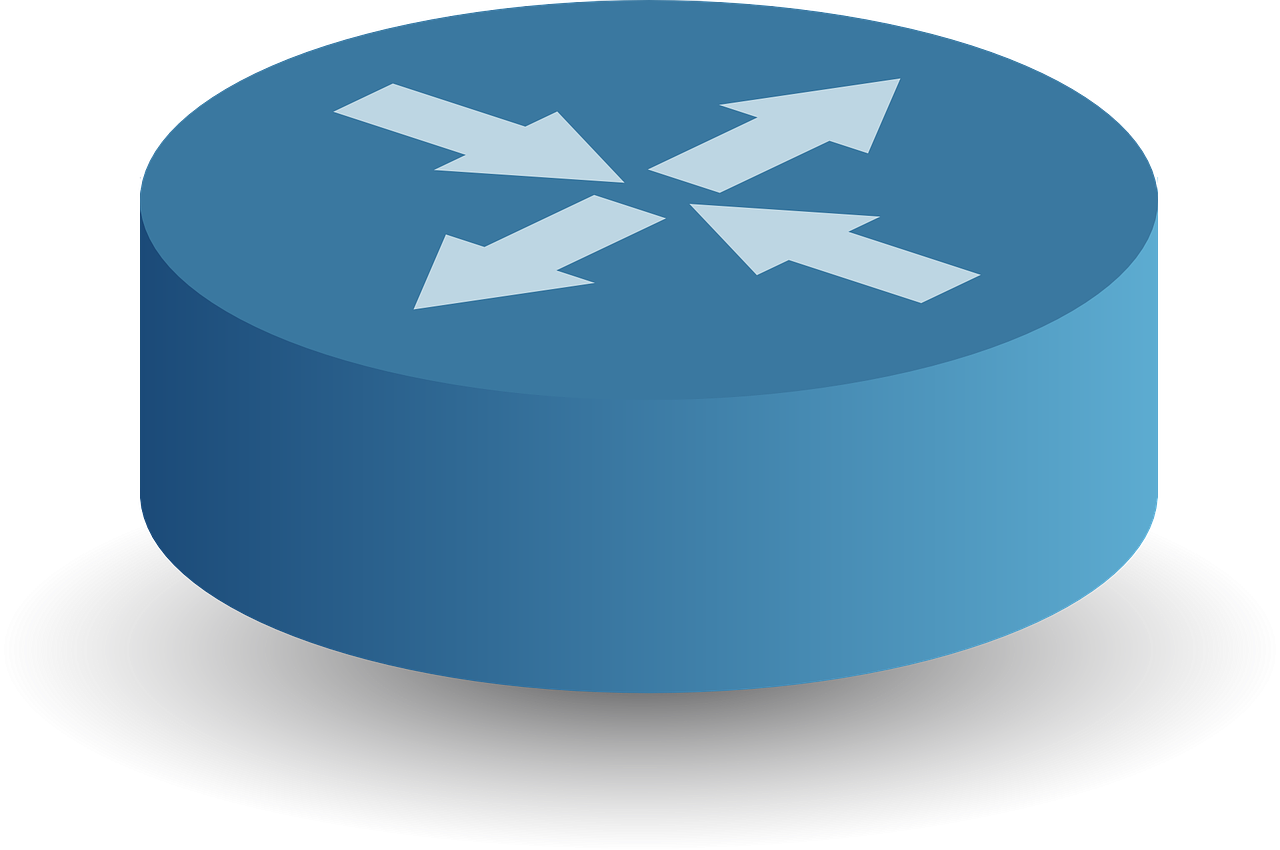
\includegraphics[width=42.75pt,height=39.38pt]{figures/router-29825_1280.png}};
%Image [id:dp3067390553920406] 
\draw (194.5,340.25) node  {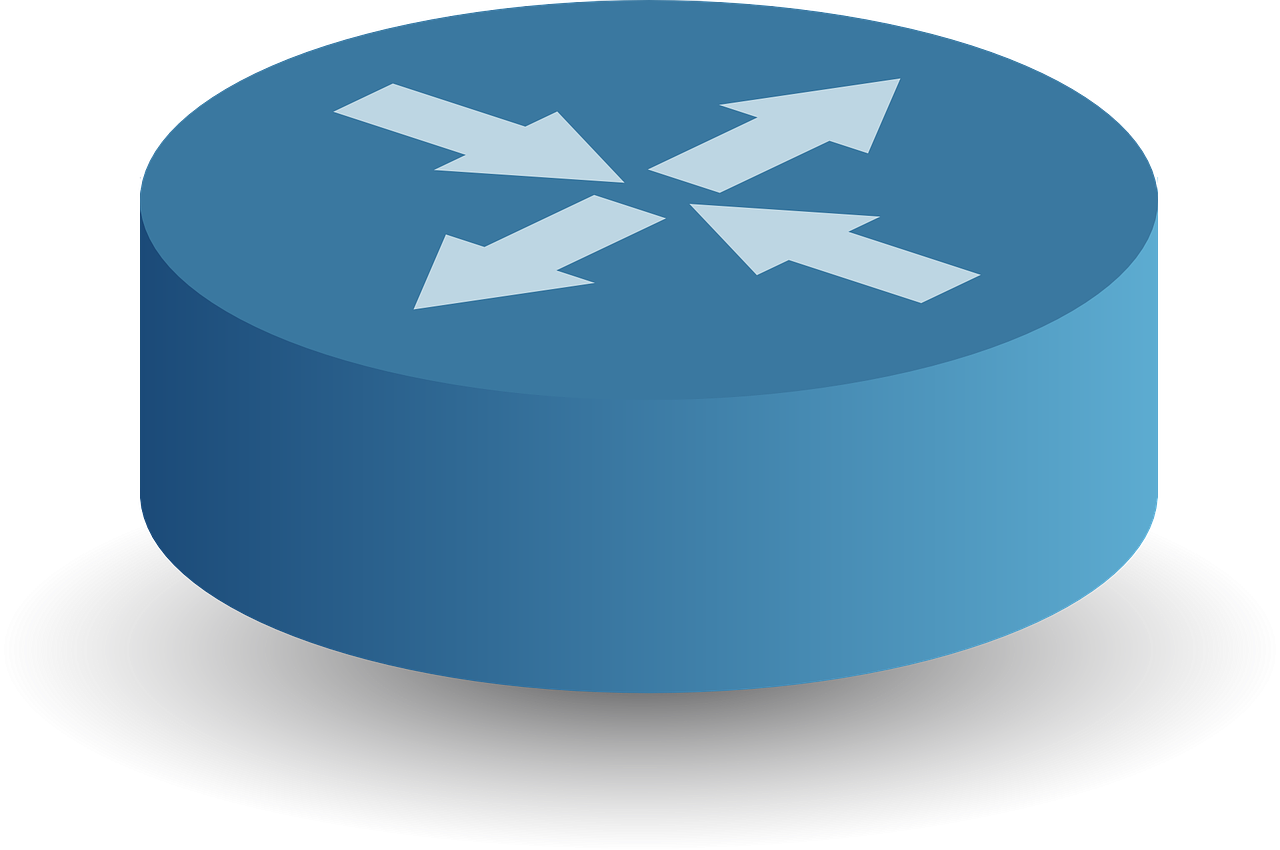
\includegraphics[width=42.75pt,height=39.38pt]{figures/router-29825_1280.png}};
%Image [id:dp24035408652285217] 
\draw (454.5,340.25) node  {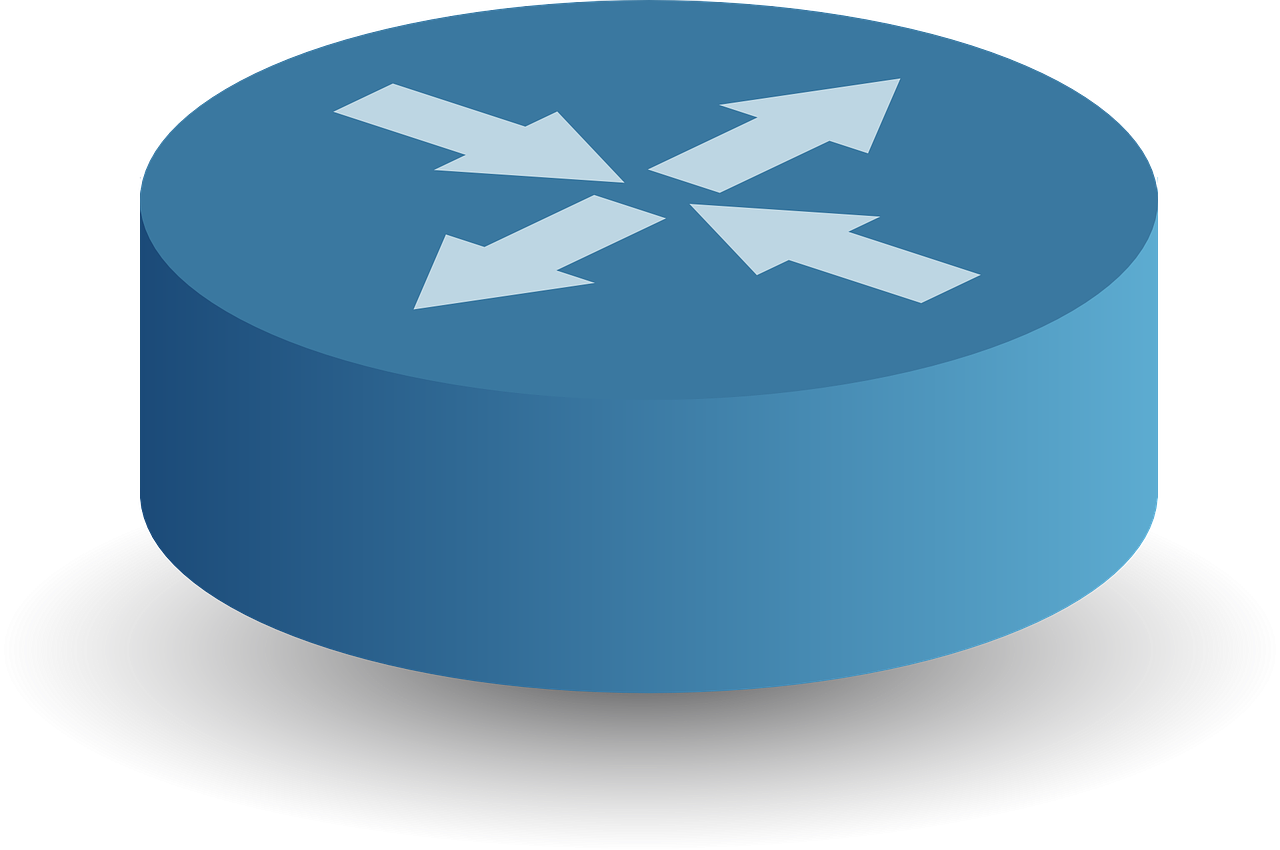
\includegraphics[width=42.75pt,height=39.38pt]{figures/router-29825_1280.png}};
%Image [id:dp7735606932716308] 
\draw (404.5,296.25) node  {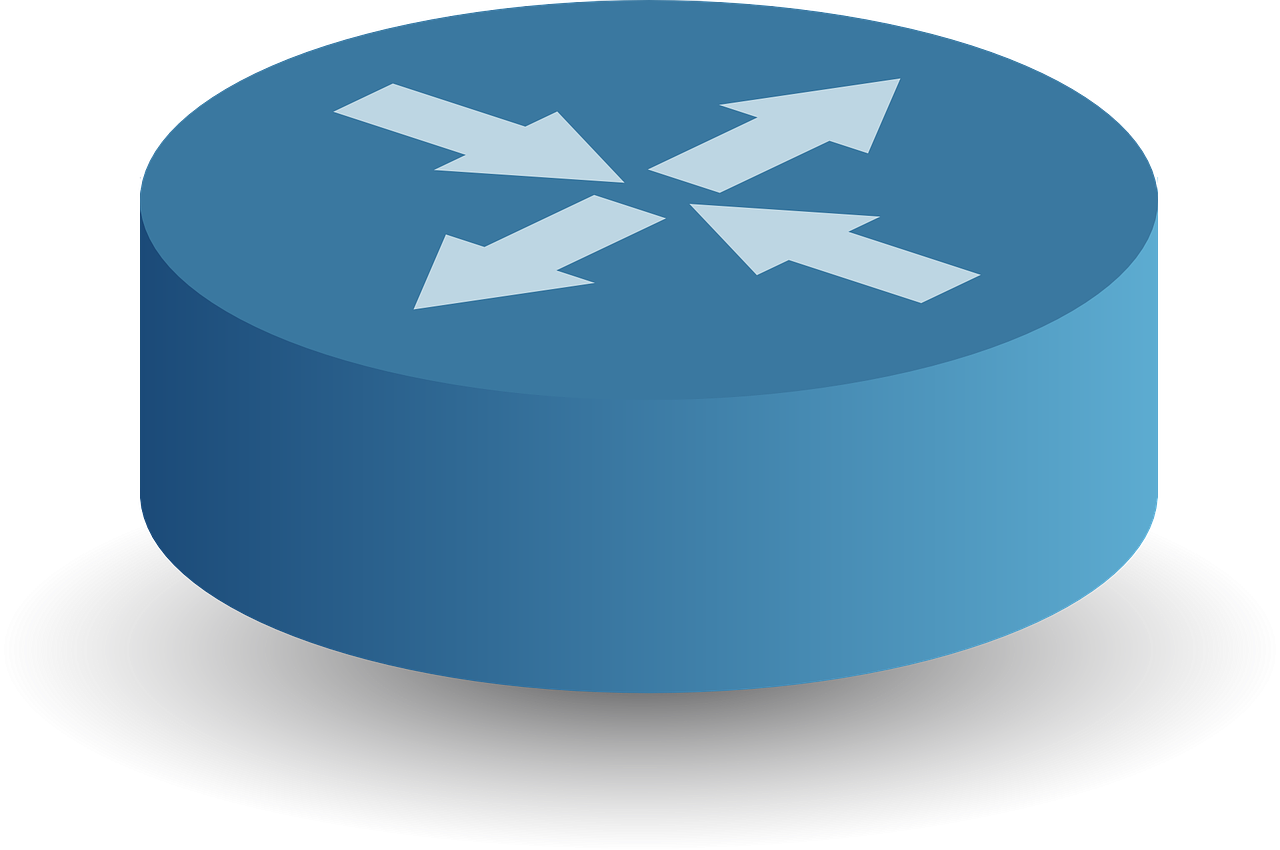
\includegraphics[width=42.75pt,height=39.38pt]{figures/router-29825_1280.png}};

% Text Node
\draw (315.27,96.53) node  [align=left] {SDN Applications};
% Text Node
\draw (315.03,121.77) node  [align=left] {Northbound API};
% Text Node
\draw (314.77,217.02) node  [align=left] {Southbound API};
% Text Node
\draw (315.27,169.4) node  [align=left] {SDN Controller};


\end{tikzpicture}

\caption{Software Defined Networking Architecture}
\label{fig:SDN-archi}
\end{figure}

The programmability of the network has given developers a lot of flexibility to design new services and network applications that will run on top of the SDN controller.
For instance, an application can prioritize how each customer's traffic should be processed, following specific Quality of Service (QoS) requirements.
Another example is a firewall that may decide to drop all the packet from a specific source because of a Denial of Service (DoS) attack.
Applications can interact with the SDN controller via the Northbound API.
Usually, SDN controllers implement a REST API for these interactions~\cite{onos-Berde2014a,opendaylight,floodlight}.
OpenFlow~\cite{Openflow-McKeown2008} (OF) is considered the standard implementation of the Southbound Interface, with numerous vendors supporting it in their products.
OpenFlow provides a Southbound interface to communicate with network equipments and to install specific configurations using a match-action formalism.
Figure~\ref{fig:matching-fields} summarizes the different OF header fields a flow can be matched against.

\begin{figure}[h]
    \centering
    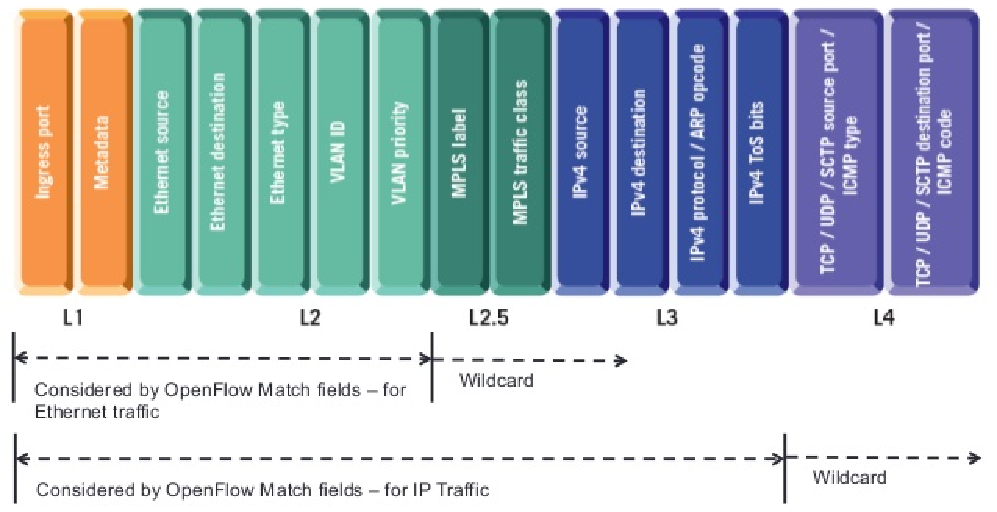
\includegraphics[scale=0.7]{figures/openflow-matchfields.pdf}
    \caption{OpenFlow matching fields~\cite{openflow-matchfields}}
    \label{fig:matching-fields}
\end{figure}

\subsubsection{Network Virtualization using SDN}
\label{def:netvirt}

For decades hypervisors have enabled the sharing and isolation of physical resources among several virtual machines.
Multiple users can run their own operating system simultaneously over a single physical machine.
On the other hand, virtualization of the network resource was implemented with VLANs, MPLS and VRF primitives, all of which were limited in terms of programmability and adaptability. The emergence of SDN and its flexibility for the design of network applications has been leveraged to give the network resource a suitable virtualization solution.

Figure~\ref{fig:virt-archi} illustrates the differences between a classic SDN environment and an SDN virtualization infrastructure. In Figure~\ref{fig:virt-archi} (a), different applications will be deployed on the SDN controller and will impact the whole physical network.
In Figure~\ref{fig:virt-archi} (b), the network hypervisor abstracts the view of the physical infrastructure into virtual networks to the end users (also referred to as tenants).
Each tenant will be able to deploy its applications on his own virtual network, that will in turn only impact the physical resources associated to it.

\begin{figure}[ht]
    \centering
    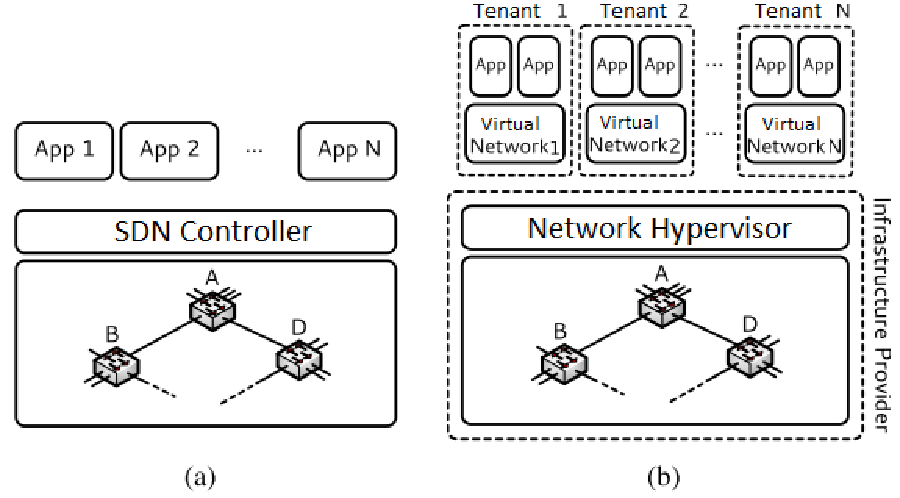
\includegraphics[scale=0.9]{figures/virt-archi.pdf}
    \caption{SDN infrastructure (a) vs. Virtualization infrastructure (b) from VeRTIGO~\cite{VeRTIGO-Corin2012a}}
    \label{fig:virt-archi}
\end{figure}


The process of mapping a virtual network with its underlying resources is referred to as Virtual Network Embedding (VNE), and is illustrated in Figure~\ref{fig:VNE}.
When a user requests a virtual network, he specifies the topology he needs, how much bandwidth is required for the links and possibly other constraints such as the geographical location of the physical resources.
The role of the VNE is to determine which resources are suited for this request, while optimizing the number of virtual networks that can be accepted in the infrastructure.
Moreover, the hypervisor is in charge to provide isolation between tenants, preventing them from interacting with other tenants' virtual networks. Isolation covers either the resources allocated to tenants, such as bandwidth, switch CPU or flow tables memory, but it also includes the topology itself so a tenant cannot manipulate traffic that does not belong to him.

Two main information are used by tenants of the virtualization infrastructure, the address space and the flowspace.\\
\textbf{The address space} is the set of IP addresses that a tenant can assign to the hosts in his virtual network.\\
\textbf{The flowspace} is the set of header parameters the tenant can use when deploying flow rules to configure his virtual network (see Figure~\ref{fig:matching-fields}). The hypervisor may restrict the use of certain headers because the virtualization already uses them as internal identifiers.
For instance, the VLAN PCP field is sometimes used for this purpose.

Providing a virtual network to the tenant can be done in three different ways, by slicing the physical infrastructure, by mapping it with the related physical resources or by providing an API to the tenant.\\
\textbf{A slice} is the set of resources allocated to a virtual network.
Slicing the physical infrastructure consists in presenting the tenant with only a small part of the infrastructure while hiding the rest of the network equipments.
The hypervisor gives tenants a direct access to the network nodes composing the slice, and the flow rules installed by the tenant will be rewritten to match the flow space he has been allocated.\\
The term slice is also found in the literature to describe the subdivision of a single physical resource. For instance, a slice can be a subdivision of a physical node corresponding to a specific tenant.\\
\textbf{Mapping} the virtual network with the physical infrastructure is an approach differing from network slicing by presenting an arbitrary network to the tenant while maintaining a mapping between the virtual elements used by the tenant and the physical resources they correspond to.
Similarly to slicing, when a tenant will interact with his virtual network, the hypervisor will be tasked to translate the identifiers and parameters used in the virtual network into the corresponding ones from the physical infrastructure.\\
\textbf{Providing} an API to the tenant allows the network hypervisor to have a better control over the capacities a tenant has on his virtual network. This extra abstraction layer can be used to limit the interactions of a tenant with his own virtual network or to alleviate existing limitations a tenant has to deploy network applications on top of his virtual network. 
\begin{figure}[ht]
\centering



\tikzset{every picture/.style={line width=0.75pt}} %set default line width to 0.75pt        

\scalebox{0.7}{\begin{tikzpicture}[x=0.75pt,y=0.75pt,yscale=-1,xscale=1]
%uncomment if require: \path (0,434.5); %set diagram left start at 0, and has height of 434.5

%Rounded Rect [id:dp5238736497415925] 
\draw  [fill={rgb, 255:red, 242; green, 175; blue, 175 }  ,fill opacity=1 ] (292,78.23) .. controls (292,67.98) and (300.31,59.67) .. (310.57,59.67) -- (524.43,59.67) .. controls (534.69,59.67) and (543,67.98) .. (543,78.23) -- (543,133.93) .. controls (543,144.19) and (534.69,152.5) .. (524.43,152.5) -- (310.57,152.5) .. controls (300.31,152.5) and (292,144.19) .. (292,133.93) -- cycle ;
%Straight Lines [id:da8274436550735994] 
\draw    (336,121.5) -- (497,116.67) ;


%Image [id:dp7319392175317063] 
\draw (327,120.5) node  {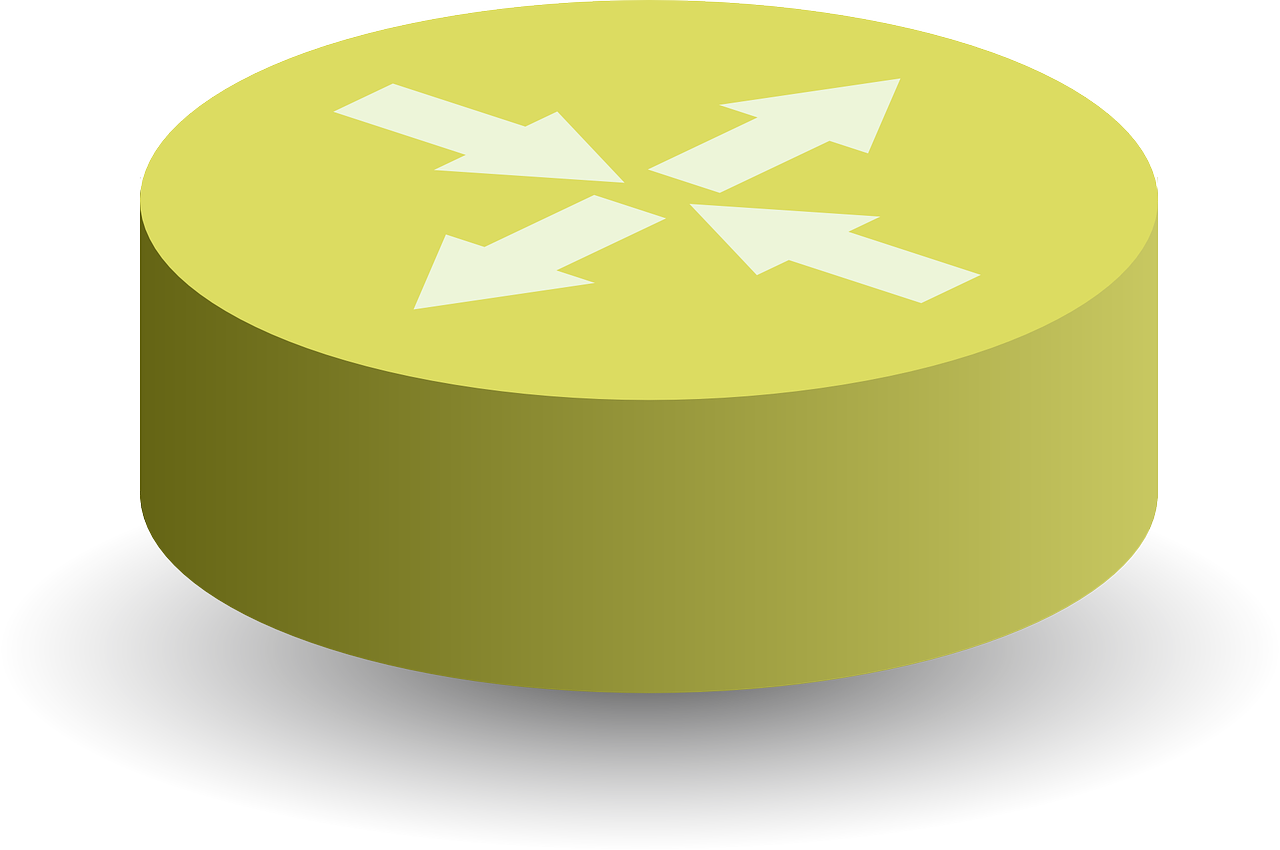
\includegraphics[width=52.5pt,height=52.5pt]{figures/router-158644_1280.png}};
%Image [id:dp370061399936939] 
\draw (412.5,120.5) node  {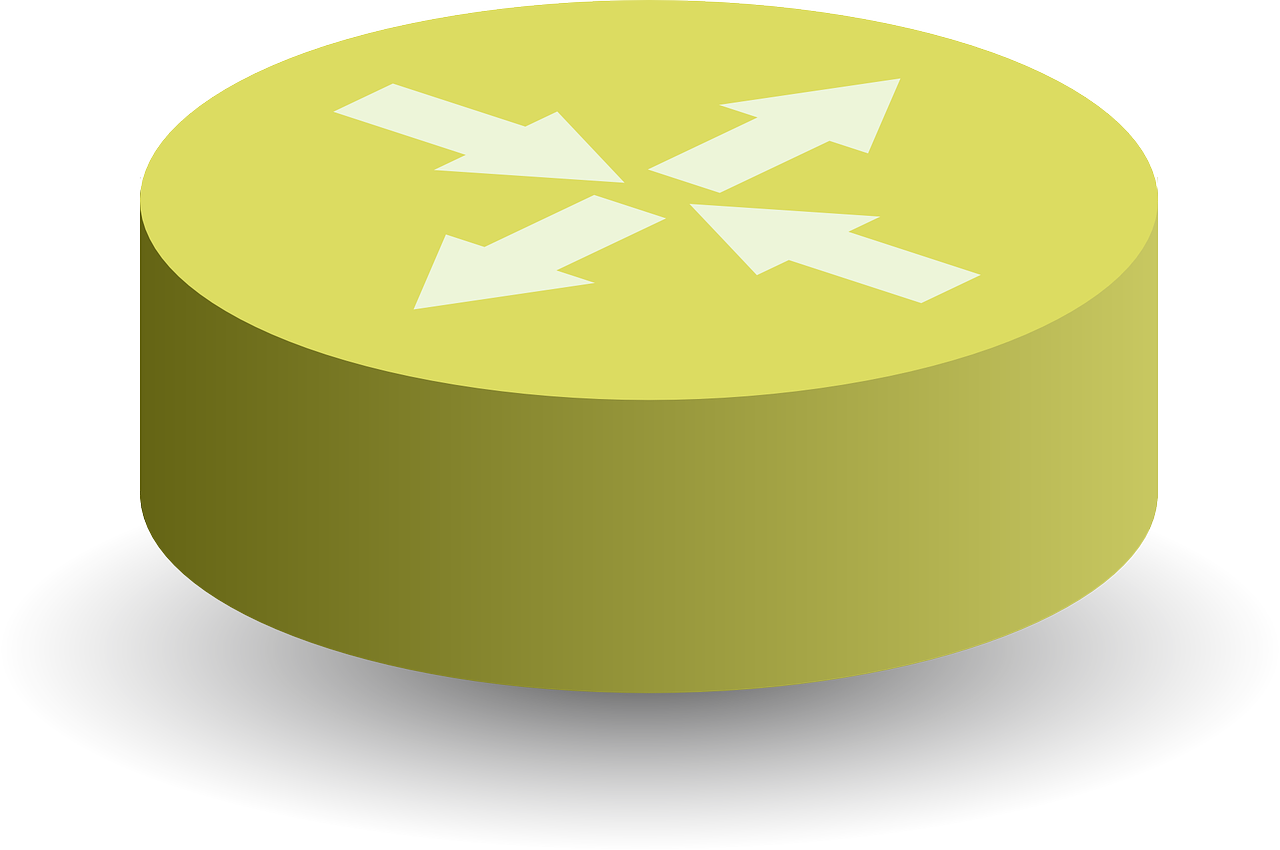
\includegraphics[width=52.5pt,height=52.5pt]{figures/router-158644_1280.png}};
%Image [id:dp4531875445870204] 
\draw (502,120.5) node  {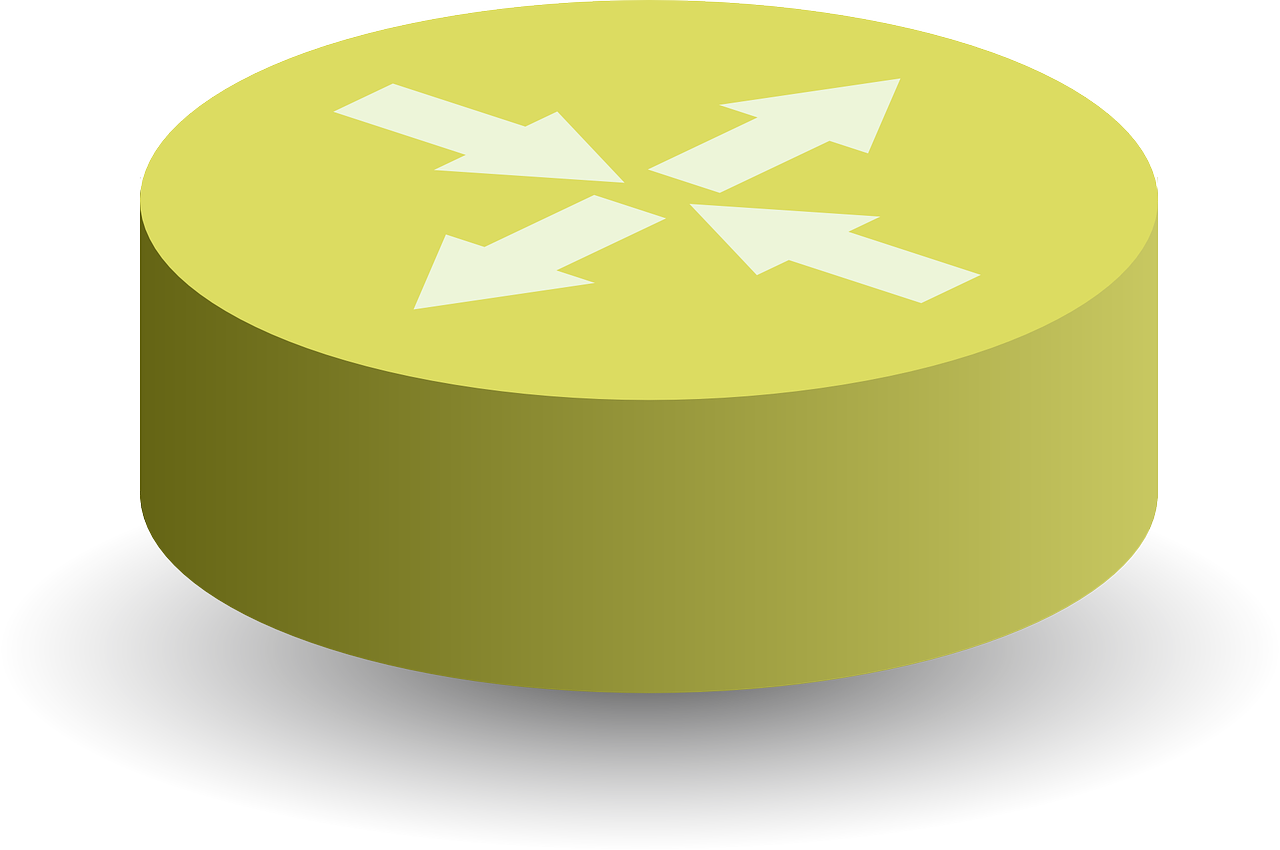
\includegraphics[width=52.5pt,height=52.5pt]{figures/router-158644_1280.png}};

%Rounded Rect [id:dp47820441471440045] 
\draw  [fill={rgb, 255:red, 255; green, 248; blue, 177 }  ,fill opacity=1 ] (46,95.27) .. controls (46,75.05) and (62.39,58.67) .. (82.6,58.67) -- (198.4,58.67) .. controls (218.61,58.67) and (235,75.05) .. (235,95.27) -- (235,205.07) .. controls (235,225.28) and (218.61,241.67) .. (198.4,241.67) -- (82.6,241.67) .. controls (62.39,241.67) and (46,225.28) .. (46,205.07) -- cycle ;
%Straight Lines [id:da6763053778165418] 
\draw    (76,150.67) -- (186,104.67) ;


%Image [id:dp8140812900187272] 
\draw (81,154.5) node  {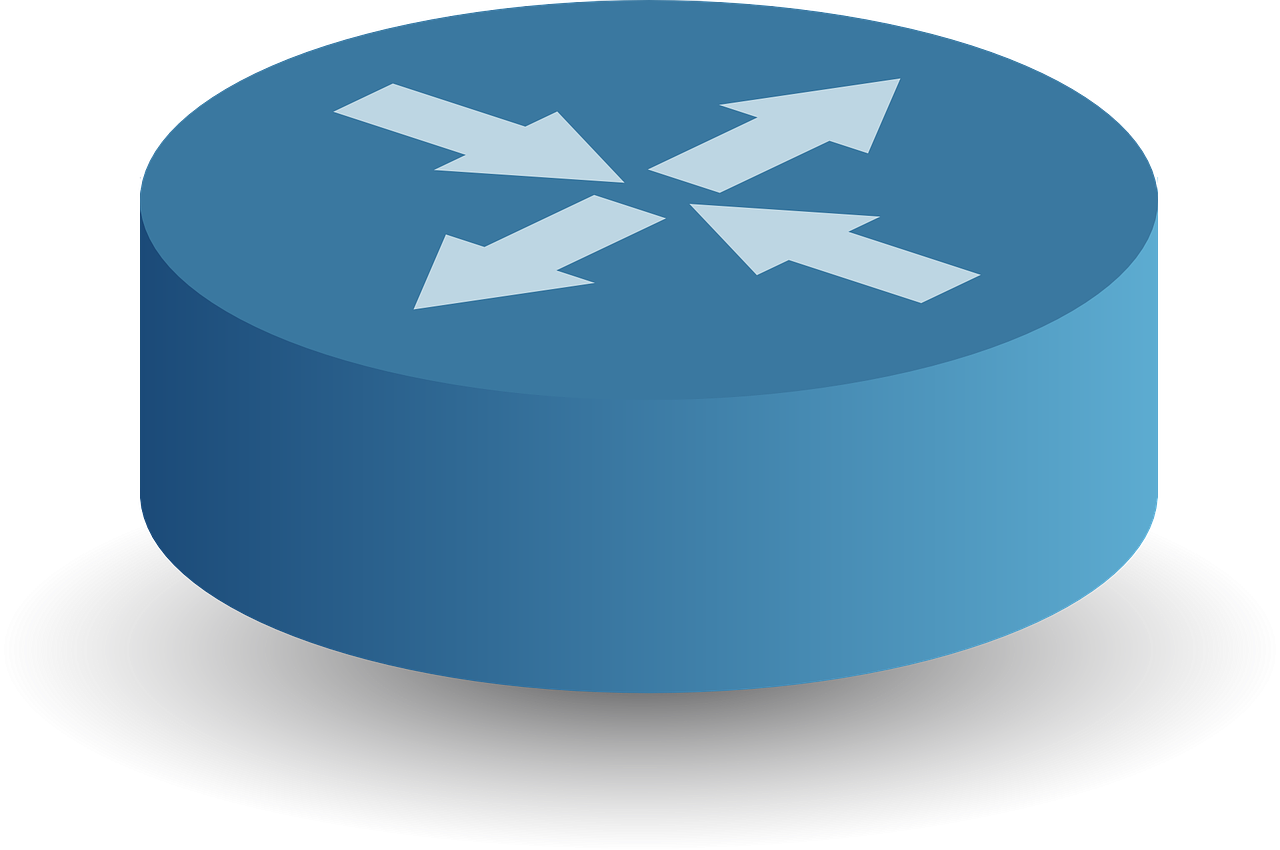
\includegraphics[width=52.5pt,height=52.5pt]{figures/router-29825_1280.png}};
%Image [id:dp7802067738931798] 
\draw (185,100.5) node  {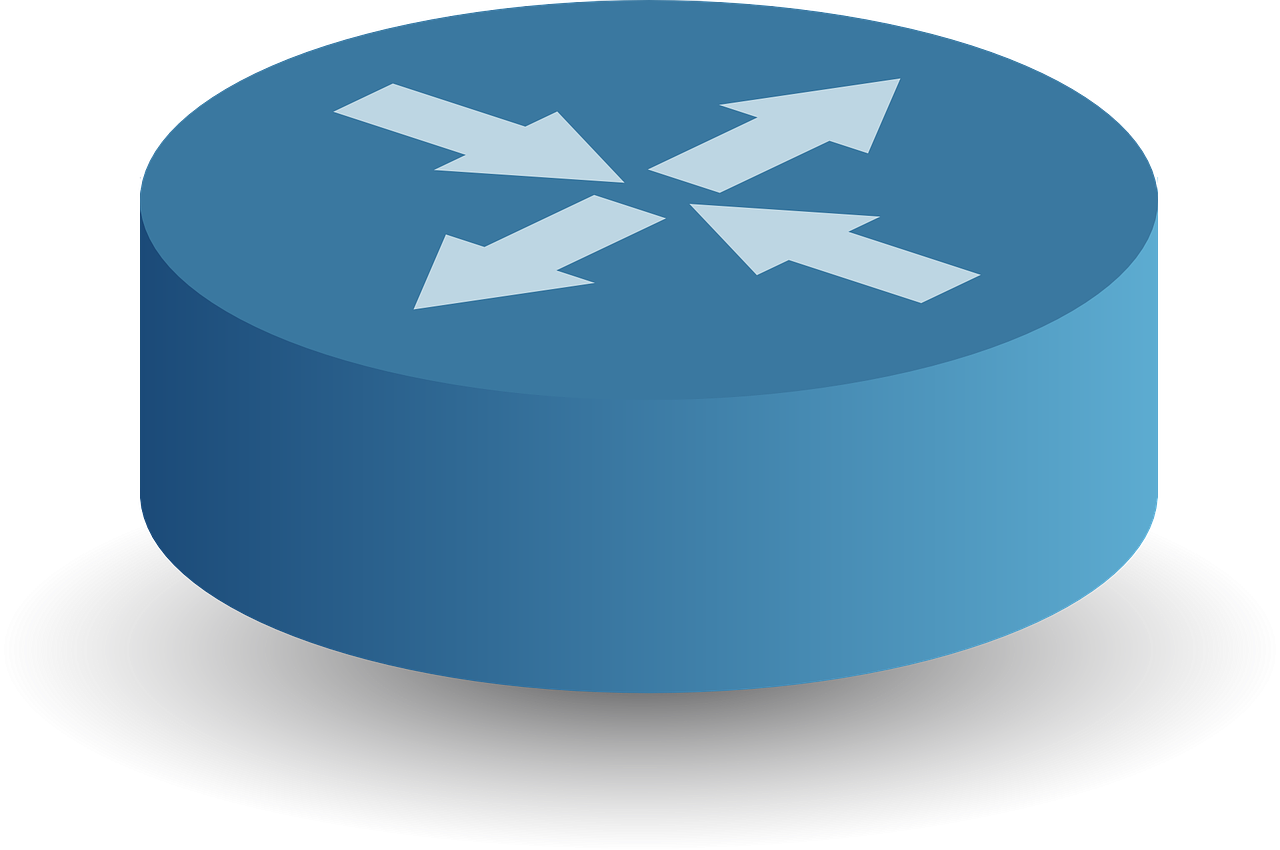
\includegraphics[width=52.5pt,height=52.5pt]{figures/router-29825_1280.png}};

%Straight Lines [id:da4951165105339822] 
\draw    (101,170.17) -- (158,195.67) ;


%Image [id:dp7416941722348419] 
\draw (156,208.5) node  {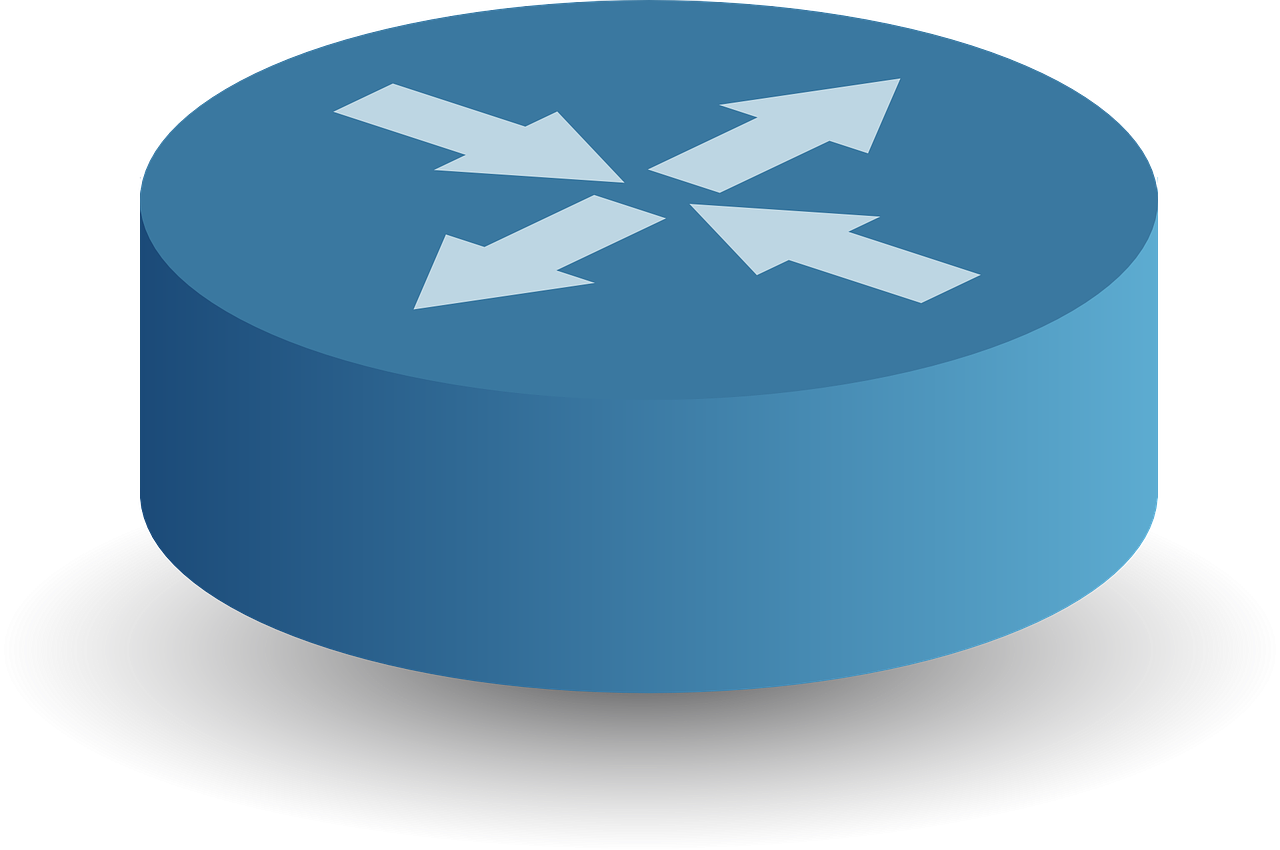
\includegraphics[width=52.5pt,height=52.5pt]{figures/router-29825_1280.png}};

%Rounded Rect [id:dp24159584532295242] 
\draw  [fill={rgb, 255:red, 184; green, 233; blue, 134 }  ,fill opacity=1 ] (27,297.47) .. controls (27,282.11) and (39.45,269.67) .. (54.8,269.67) -- (602.2,269.67) .. controls (617.55,269.67) and (630,282.11) .. (630,297.47) -- (630,380.87) .. controls (630,396.22) and (617.55,408.67) .. (602.2,408.67) -- (54.8,408.67) .. controls (39.45,408.67) and (27,396.22) .. (27,380.87) -- cycle ;
%Straight Lines [id:da4431598038778879] 
\draw    (99,327.67) -- (234,300.67) ;


%Straight Lines [id:da13869241806959443] 
\draw    (100,342.67) -- (191,365.67) ;


%Straight Lines [id:da638319369024069] 
\draw    (194,372.67) -- (388,325.67) ;


%Straight Lines [id:da0876024287705166] 
\draw    (234,300.67) -- (378,309.67) ;


%Straight Lines [id:da03053485372734699] 
\draw    (404,319.67) -- (522,306.67) ;


%Straight Lines [id:da8278064324522899] 
\draw    (395,339.67) -- (497,375.67) ;


%Image [id:dp619468693007916] 
\draw (90,342.5) node  {
\includegraphics[width=52.5pt,height=52.5pt]{figures/router-30140_1280.png}};
%Image [id:dp8001089418713573] 
\draw (180,373.5) node  {
\includegraphics[width=52.5pt,height=52.5pt]{figures/router-30140_1280.png}};
%Image [id:dp9285996053263255] 
\draw (220,310.5) node  {
\includegraphics[width=52.5pt,height=52.5pt]{figures/router-30140_1280.png}};
%Image [id:dp3146785253004203] 
\draw (406,324.5) node  {
\includegraphics[width=52.5pt,height=52.5pt]{figures/router-30140_1280.png}};
%Image [id:dp3289010965024106] 
\draw (535,313.5) node  {
\includegraphics[width=52.5pt,height=52.5pt]{figures/router-30140_1280.png}};
%Image [id:dp13463717449619406] 
\draw (535,386.5) node  {
\includegraphics[width=52.5pt,height=52.5pt]{figures/router-30140_1280.png}};
%Straight Lines [id:da2794186668497024] 
\draw [line width=1.5]  [dash pattern={on 1.69pt off 2.76pt}]  (83,177.17) -- (82,307.97) ;


%Straight Lines [id:da3468403679668073] 
\draw [line width=1.5]  [dash pattern={on 1.69pt off 2.76pt}]  (158,228.17) -- (160,341.97) ;


%Straight Lines [id:da6099923036688548] 
\draw [line width=1.5]  [dash pattern={on 1.69pt off 2.76pt}]  (196,123.17) -- (197.2,280.27) ;


%Straight Lines [id:da9880025849572002] 
\draw [line width=1.5]  [dash pattern={on 1.69pt off 2.76pt}]  (318,140.17) -- (235.6,279.47) ;


%Straight Lines [id:da6145453947319308] 
\draw [line width=1.5]  [dash pattern={on 1.69pt off 2.76pt}]  (516,141.17) -- (515.6,283.07) ;


%Straight Lines [id:da41673177695849406] 
\draw [line width=1.5]  [dash pattern={on 1.69pt off 2.76pt}]  (413,143.17) -- (410.4,290.27) ;



% Text Node
\draw (105,397.5) node [scale=0.9] [align=left] {Physical Infrastructure};
% Text Node
\draw (89,74.5) node  [align=left] {{\small vSDN1}};
% Text Node
\draw (327,70.5) node [scale=0.9] [align=left] {{\small vSDN2}};


\end{tikzpicture}}


\caption{Principle of Virtual Network Embedding.}
\label{fig:VNE}
\end{figure}

\subsubsection{Virtual Network Migration}
The migration of a Virtual Network is a maintenance process used to change the embedding of the virtual network. 
This correspond to the allocation of a set of physical resources to partially or totally replace the original embedding of the virtual network.
There are several reasons to migrate a Virtual Network, requests acceptance ratio optimization, resource failure, attacks on the infrastructure.
Reallocating resources to a Virtual Network is done to improve the general acceptance ratio of Virtual Networks in the infrastructure.
In the event of a physical failure or an launching resource depletion attacks, the physical resources cannot support the operation of the virtual networks and the migration is necessary to maintain the availability of the service provided to the customer.

In a SDN virtualization environment, the migration of a Virtual Network consists in computing new OF rules and install them in the newly allocated physical resources.
We do not consider here the internal aspect of the migration in the network hypervisor, which corresponds to updating the different information about the topology, the allocation requirements and other mechanisms that are specific to the implementation of each network hypervisor.

From a network perspective, the migration process can be summarized by the following steps:

\begin{itemize}
    \item \textbf{Request for migration} The hypervisor determines which Virtual Networks must be migrated.
    \item \textbf{Embedding computing} The hypervisor determines the new set of physical resources.
    \item \textbf{OF rules deployment} The hypervisor installs new OF rules while removing those who belong to the old embedding.
\end{itemize}

The order in which the hypervisor installs and removes OF rules is considered by some solutions that we will cover later on this chapter.

\newpage
\section{State of the Art}
\label{sec:sota}
% \FC{This introduction is not meant to stay, it's just a rough explanation of the plan}
% We know for a fact that there is not much work done on the security of VN migration.
% In order to prove the usefulness of my work, I start with a SotA of VM migration, and the related security issues.
% THe aim is to show that there are vulnerabilities and attacks existing with VMs that are inherently relevant with VN migration.
% Then the topic of SDN virtualization, listing existing hypervisor. (Stating there was no usable tool ?)
% Then we go for the security of VN migration. Since there is not much about the security of the process in itself, it will most likely be about secure VNE etc.
% We have now provided enough content to justify why the problem we work on is worth it.
% Now I will introduce the topics/tools/techniques I used to answer it.

% We start from the formal models. The very first work I did was to determine whether there was an adequate existing model, if it could be extended to fit my purposes. 
% The second part of the work was to do the monitoring of network events, in order to connect these to the formal model. This part is partly covered in the SDN section of SotA.
% The last part was the verification of the security properties using the network trace and the theorem prover.

% The Game Theory section should outline the properties I wanted to use for my game. This should also lead to an obvious lack of ``advanced" models solving solutions. Obviously, there are also a lot of dead ends in GT that lead to going on using MDP instead. I don't know if this should be here.

% Then we have the RA problem, with the different methodologies. This should look like the work we've done for NCA 2019 but with a better organisation, as suggested by Christophe. I've added attack graphs because I have some documents in Mendeley I want to go through and see their relevance. This section might disappear.
In this section, we provide a literature review of the different topics studied in this thesis.
First of all, we examine the existing network hypervisors, and detail them under the scope of network migration with regard to the type of abstraction they provide.
Then we will specifically address the topic of virtual network migration, and the purpose of the different solutions.
The last topic considered here is related to the resource allocation problem and we will present 
security problems encompassed in it.

\subsection{Network virtualization using SDN}

Network virtualization has leveraged the use of SDN to provide a flexible abstraction layer to service providers. In this section, we first propose classification criteria for network hypervisors and then evaluate existing hypervisors against this classification. We will propose a reference architecture for network hypervisors implementing a secure network migration feature, based on existing solutions.

\subsection{Classification criteria}
We study existing network hypervisors through the prism of virtual network migration.
The scope is restricted to general purpose platforms and equipments to provide the network virtualization service. Therefore, hypervisors using specific technologies such as WiFi, radio frequencies or optical fiber. are out of the scope of this work.

% \GB{please rewrite the below paragraph}
We categorize existing hypervisors based on the type of abstraction used to present Virtual Networks to the tenants, and whether or not the Virtual Network migration process is implemented in the considered hypervisor.

\begin{itemize}
\item \textbf{Abstracting the physical infrastructure}
The first criterion used to classify existing hypervisors is concerned with how the virtual network is presented to the tenant. We have presented in Section~\ref{def:netvirt} the possible abstractions: slicing the infrastructure, mapping each Virtual Network with their allocated physical resources, or exposing a specific API to the tenant.

\item \textbf{Migrating virtual networks}
The second criterion we consider is whether or not the network hypervisor has implemented the migration of a virtual network in case of a physical failure or an attack on the infrastructure.

\item \textbf{Tenant identification}
An important aspect of the virtualization is how the network hypervisor implements the identification of each tenant in the infrastructure, to determine how to process the network traffic.

\item \textbf{Resource Isolation}
The network hypervisor enforces isolation between the different tenants.
This isolation ensures that each tenant is served with the required amount of resources.
\end{itemize}


\subsubsection{Existing hypervisors}
\label{sec:existing-nhv}
In this section we describe the existing hypervisors and their ability to implement Virtual Network Migration.

\paragraph{FlowVisor}

FlowVisor~\cite{FlowVisor-Sherwood2009} is the first SDN hypervisor implemented.
FlowVisor provides Virtual Networks by slicing the physical infrastructure, and providing each tenant with a set of physical resources.

Virtual networks are defined as a set of links between physical SDN switches.
These links will only match the traffic belonging to the tenant.
FlowVisor introduce them as flowspace and each flowspace maps a tenant with a physical node and a specific match-action criteria for the traffic.
For a tenant, the collection of these flowspaces is called a slice and represent their virtual network. 
The tenant will then connect their SDN controller to the slice, enabling them to interact with their virtual network.

FlowVisor enforces isolation between tenants by acting as a proxy between them and the physical infrastructure.
FlowVisor abstracts the physical architecture by showing each tenants only the resources that have been allocated to them.
When an OpenFlow message is sent from a physical node to the controller, FlowVisor will intercept the message and forward it only to the tenants with a Virtual Network using this node in their substrate.
Similarly, when a tenant wants to deploy an OpenFlow rule (OF rule) on a physical node, FlowVisor will intercept it and rewrite match and actions fields so the rule only affects the virtual network and not all the ongoing traffic.

Flowvisor enforces isolation of bandwidth, topology, switch CPU, flowspace, flow entries tables and the southbound interface communications. Authors have evaluated the performance of these isolations in~\cite{FlowVisor-Sherwood2009}.
However, FlowVisor lacks to major components related to virtualization, arbitrary topologies and virtual network migration.
These aspects have been tackled in hypervisors based on FlowVisor.

\paragraph{ADVisor}
ADVisor~\cite{ADVisor-Salvadori2012} is based on FlowVisor and tackles two design issues introduced with FlowVisor.
The first contribution is the implementation of arbitrary virtual topologies.
Instead of slicing physical resources and presenting them to the tenants, 
The virtualization completely decouples the abstract view of the virtual network from the physical resources supporting it.
A virtual link between two virtual nodes might in fact be composed of several physical links. The role of ADVisor will be to hide these intermediate nodes from the tenant.

The second contribution of ADVisor consists in the sharing of the flowspace proposed by FlowVisor.
Originally, the definition of a flowspace would restrict the manipulation of a certain type of traffic (\eg port 80, 10.0.0.0/24 block) to only one tenant.
Giving access of one flowspace to two different tenants would break the isolation and allow one to control and alter the traffic of the other.

\paragraph{VeRTIGO}
VeRTIGO~\cite{VeRTIGO-Corin2012a} is an extension of the work done with ADVisor and offers two different types of virtual networks.
Either the tenant will have the full control over the virtual network (including traffic engineering techniques etc.) or he will be presented with a single node and leaves the handling of network operations to the service provider.
This abstract view is often called ``Big Switch Abstraction".
It provides networking to a tenant who is not interested in handling network operations himself.

VeRTIGO implements virtual network migration using a component called VT Planner. The VT Planner consists in a set of precached virtual topologies that will be deployed in case of link failure. In case of link congestion of physical failure, the VT Planner will migrate the virtual network by deploying the configuration rules into the new network equipments.

\paragraph{Enhanced FlowVisor}
Enhanced FlowVisor~\cite{EnhancedFV-Min2012} extends FlowVisor by implementing a minimum guaranteed bandwidth feature. It ensures that each tenant of a virtual network will be served with the required amount of bandwidth for all the links in his topology. Information about virtual networks, tenants information etc. are stored in a database. When a new request for a virtual network is received, a potential physical substrate will be mapped with the request. Then Enhanced FlowVisor will query the database to check if each link in the physical substrate can cover for the requested bandwidth of the virtual network. If it cannot, then the request is denied. 
The flowspace used in this solution is based on 3 bits of the VLAN PCP field which restricts the total number of tenants to 8.
Enhanced FlowVisor is based on the NOX controller and uses HP ProCurve switches using the Guaranteed Minimum Bandwidth feature.

\paragraph{Slices Isolator}
Slices Isolator~\cite{SlicesIsolator-El-Azzab2011} is an hypervisor providing resource isolation between slices. A slice is defined as a subdivision of a physical switch, to which flows will be affected. Slices Isolator provides isolation for interfaces, flow processing and memory. Interface isolation consists in either providing a dedicated network interface to a slice or to aggregate incoming traffic to one interface and then distributing the control to the different tenants. Processing isolation defines which flows will be processed using the same rules. Each flow is splitted into two subflows, one is discarded and the other is processed. This helps reducing the size of processing tables but if a bad rule is added it can compromise the expected behavior of the system. Therefore, processing isolation works by determining if the addition of the new rule does not conflict with the previous rules. The new rule is valid if either the new flow does not intersect with any of the existing flows or if it does, it is part of the discarded section of the flow. Finally, memory isolation is implemented with queuing algorithms for the traffic, ensuring a slice does not overload its allocated resources. 

\paragraph{Double FlowVisor}
Double FlowVisor~\cite{DoubleFV-Yin2013} combines two instances of FlowVisor to virtualize a multi-domain network and provide a unified view of the virtual network. The first instance of FlowVisor is used to hide the heterogeneity of the different network domains. These domains are connected together and are abstracted and a NOX controller~\cite{nox-gude2008} is connected to FlowVisor.
Then, the second FlowVisor instance will connect NOX with the tenants' applications. This instance maintains the embedding between virtual resources and the physical substrate, and translates commands sent by the tenant into commands deployed in the physical infrastructure. In addition to that, the second FlowVisor instance is in charge to tag each flow with an APP-ID related to the tenant.

\paragraph{Compositional Hypervisor}
The aim of Compositional Hypervisor~\cite{CompositionalHypervisor-Jin2014} is to provide an homogeneous layer between SDN controllers and tenants application.
Each application is designed to work with a specific SDN controller and is based on a specific programming language. Therefore, it is next to impossible for a tenant to concurrently run different applications from different environments because they will conflict with each other. Compositional Hypervisor sits between the physical infrastructure and the SDN applications used by tenants.
The OF rules sent by an application define a policy that the tenant will then be able to combine with other policies using a provided arithmetic.
This arithmetic allows to have policies being enforced either in parallel or sequentially. This composition simplifies the OF rules deployed in each switch by providing a unique list of prioritized OF rules. When one of the policies is update, the hypervisor will recompute the updated policy depending on whether a rule has been added/removed/modified.

\paragraph{CoVisor}
CoVisor~\cite{CoVisor-Jin2015} extends Compositional Hypervisor~\cite{CompositionalHypervisor-Jin2014} by making two significant contributions.
The first one is a novel policy combination algorithm that will focus on the performance of the policy deployment in terms of packets send and computation time.
CoVisor exploits the policies being composed to generate specific data structures instead of R-tree-based data classifiers.
Regrouping composed policies based on the common fields they affect reduces the number of rules pair considered at compilation time.
Similarly, they correlate common attributes between policies to serve as indexes for storage. Determining the intersection of the matching fields for two policies determines the index storage for the composed policy.
This algorithm also support the case where a single physical node spans multiple virtual switches.

The second contribution is related to the view the hypervisor gives to each application.
Due to security concerns, CoVisor present an abstract view of the topology based on the needs of the application. 
For instance, a firewall may only see the infrastructure as a big switch since the incoming traffic should be dropped at the ingress point of the network.
Similarly, a routing application will require full access to the network to determine the optimal routing paths.
CoVisor also limits the actions available to each application using a fine-grained control over the capacities of each controller.
For example, a MAC learner application should only match packets based on MAC addresses, or a firewall should only be able to accept or drop packets, and not to modify them.
By design CoVisor implements two fail-over mechanisms regarding controller failures and switch failures.
Controller failure is handled by introducing a third operator in the policy composition, namely the override operator. This operator specifies which policy to apply if another fails.
In case a physical switch fails, CoVisor notifies each application impacted by the failure and redeploys required OF rules elsewhere in the network when possible.

\paragraph{FlowN}
FlowN~\cite{FlowN-Drutskoy2012} is a network hypervisor designed to provide a full abstraction of the physical infrastructure and to propose a container-based application virtualization system. 
The hypervisor serves each tenant with a custom virtual topology. The virtual topology requires a specific number of nodes and links but FlowN also implement bandwidth reservation as well as maximum latency per link. The decoupling of the virtual network from the physical substrate removes the burden of network maintenance from the tenant and leaves it to the service provider. In case of a switch or link failure, FlowN will migrate the virtual node on a new physical switch without having to notify the impacted tenants.
FlowN evaluate the time it takes to migrated nodes impacting 50 virtual networks and time never exceeds 65 ms.

FlowN also offers the full abstraction of the address space for the tenants.
Each tenant will be able to use all the header fields, and FlowN will maintain through the use of a database the mapping between the physical node address space and the virtual one. FlowN uses encapsulation at the ingress point to determine to which tenant the packet must be forwarded. Encapsulation is based on VLAN tagging, in a similar fashion to Nicira~\cite{nicira}.   
FlowN leverages the capabilities of databases to improve the performance of the mapping.

The virtualization of the control layer places FlowN between tenants' applications and the physical infrastructure. When a SDN application makes a function call, FlowN will intercept it and translate it to preserve the mapping between virtual address space and the physical address space. Since FlowN is based on the NOX~\cite{nox-gude2008} SDN controller, tenants are also limited by the capacities of this controller. 
The design of an API between applications and hypervisor is in opposition to the concept of FlowVisor~\cite{FlowVisor-Sherwood2009} where tenants directly interact with the physical nodes and FlowVisor only restrict and translate OF rules to respect the isolation requirements of the virtualization.

\paragraph{Network Hypervisor}
The Network Hypervisor~\cite{NetworkHypervisor-Huang2013} aims at providing a unified virtualization over multi-domains SDN infrastructures. Authors present a vision of the future of SDN network and how infrastructure providers, services resellers and users would work to provide a seamless virtualization service that would alleviate the maintenance operations burden from the tenants.
The ultimate goal of the Network Hypervisor is to enable HyperNets~\cite{HyperNet-Huang2013a}. HyperNets are envisioned as a sort of final form for SDN services. A user may request a virtual network to serve specific needs (\eg Video Streaming) and connect specific clients together.
The HyperNet should be able to automatically determine what are the physical resources that should be allocated in terms of positioning, computational power etc. In addition to this, HyperNets should provide routing procedures specifically design for the requested service (\ie prioritize video traffic over less relevant traffic).
In order to provide the support of said HyperNets, the Network Hypervisor provides API functions. These functions includes network discovery so they can allocate suitable physical resources close the HyperNet users as well as design a suitable topology to interconnect all participants.
Moreover, they implement a dynamic join/leave feature, where users will be allowed to connect to a SDN virtual network without being directly connected to one. The use of IP tunneling solves such connectivity issues.
Aside from these high level API functions, the role of the Network Hypervisor is to concatenate the different network resources connected to it.
This hypervisor has been implemented to work on top of the ProtoGENI~\cite{protoGENI} infrastructure.

\paragraph{AutoSlice}
AutoSlice~\cite{AutoSlice-Bozakov2012} is designed to tackle the scalability issues of a distributed hypervisor, and optimize resource consumption of physical switches to overcome specific limitations.
In~\cite{AutoSlice-Bozakov2012} authors present the basis of the AutoSlice hypervisor.
Each physical SDN infrastructure is managed by its own controller proxy (CPX).
Each CPX is in charge of accessing corresponding physical switches and translating OF rules from the virtual flowspace to the physical one.
AutoSlice instantiate virtual networks over several SDN domain and each CPX deploys the corresponding OF rules in their infrastructure.
Each CPX is in charge of migrating virtual resources within their own domain.
AutoSlice overcomes the physical limitations of Openflow switches by delegating part of OF rules storage to Auxiliary Software Datapaths (ASD).
These ASD are software switches running on ommodity servers and therefore have the sufficient resources to store all the possible OF rules.
AutoSlice uses a statistical distribution law to determine that low volume flows will generate most of the OF rules and store them in ASD. In opposition, the biggest volume flows use a minimum of OF rules and deploy them inside the physical switches.
In~\cite{AutoSlice2-Bozakov2014} authors go into more details about several design requirements they have expressed. They extend the notion of isolation between tenants by introducing a set of identifiers to prevent overlapping OF rules installed by different tenants.
The isolation of flow tables is ensured by adding a \textit{Virtual Table Identifier} thus sharing the physical flow table among the different tenants.
Similarly, all packets are marked with a \textit{Packet Identifier} so it can be mapped with th \textit{Virtual Table Identifier} and determine how the packet should be processed.
Authors also propose virtual network migration techniques based on information duplication, and highlight the potential excessive usage of flow table resources.
There is no evaluation provided in both~\cite{AutoSlice-Bozakov2012} and~\cite{AutoSlice2-Bozakov2014}.

\paragraph{NVP}
The Network Virtualization Platform~\cite{NVP-Koponen2014} (NVP) proposes a network hypervisor for multi-tenants datacenters. Instead of focusing on virtualizing the physical network of the data center, NVP provides a virtual network on top of OpenvSwitches~\cite{openvswitch} deployed in each VMWare Hypervisor. Those virtual switches are then interconnected using tunnels for end-to-end communication. The physical network is simply used as traditional networking and is assumed to possess standard capacities.
The paper makes several contributions: the implementation of the logical networks based on OpenvSwitch (OVS), the creation of a Domain Specific Language (DSL) to declare the connectivity between hypervisors, switches etc. and tackle scalability and availability issues encountered by NVP.

The logical networks proposed to a tenant in NVP consist in creating a virtual slice inside each OVS which in global sets a logical pipeline between the different VMs pertaining to the tenant.
Each VM hypervisor hosting VMs belonging to a specific tenant will instantiate a \textit{logical datapath} inside its own OVS. 
Then, for each pair of logical datapaths that have been created NVP will create a tunnel between them.
Each time an incoming packet goes through an ingress port of the hypervisor the packet will be redirected to the correct logical datapath then transmitted to the logical datapath corresponding to the destination VM.
The tenant can configure these datapaths with regard to switching, routing and security matters, similarly to traditional networking elements.
The isolation between tenants is ensured by affecting unique identifiers to each logical datapath, preventing unauthorized access to the tenant's traffic.
NVP implements failover mechanisms of physical networking elements as well as controllers by running backup nodes with similar function that will be used in case of a failure.

NVP introduces \textit{nlog}, the DSL proposed in NVP is used tackle the computational challenge of keeping up with the evolution of the forwarding state inside the logical datapaths. Changes in the forwarding state include entries and departures of tenants inside the infrastructure, migration of the different VMs, reconfiguration of logical datapaths by the tenants. \textit{nlog} presents an logical abstraction that decouples the concrete forwarding state and rules from the logic described by NVP. Note that \textit{nlog} is not used by tenants but by NVP when instantiating logical datapaths for tenants.
Tenants are provided an API to interact with NVP.
Using \textit{nlog} to describe the state of the logical abstractions enables an incremental computing of the forwarding state that is resource efficient compared to a naive implementation where any change requires the full recomputation of the forwarding state.

Scalability inside NVP is ensured by distributing computation over several logical controllers and physical controllers. Logical controllers compute the flow and tunnels corresponding to datapaths. Physical controllers are in charge of the communication with the different service nodes, gateways and hypervisors.
Sharding mechanisms are responsible for the availability of the different nodes inside the infrastructure. A sharding coordinator will monitor the signals sent by the different nodes and will promote a node to the master role if the current master fails.

The evaluation of NVP focuses on two things, the time and resources required to setup NVP in different scenarios and the available throughput based on which tunneling mechanism is used by NVP. Theses results are then followed by a serie of reflexions based on the experience gained after the implementation of NVP and how design challenges have been tackled.

\paragraph{OpenVirteX}
OpenVirteX~\cite{OpenVirteX-Al-Shabibi2014} (OVX) is a network hypervisor based on the same design as FlowVisor~\cite{FlowVisor-Sherwood2009}. OVX serves as a proxy between the tenants' controllers and the underlying physical infrastructure. OVX provides both full virtual topology abstraction and full address space abstraction. 

When a tenant requests a virtual network, he describes the different resources, nodes and links he needs.
Then OVX will determine the adequate physical substrate to embed the virtual network.
The virtual/physical resources mapping is stored by OVX and is used to present the virtual topology to the controller.
While FlowVisor will hide messages to unintended recipients, OVX intercept LLDP packets used for topology discovery. Everytime a LLDP message arrives at a virtual switch, OVX uses the mapping to determine the virtual node at the other end of the virtual link. A LLDP response is forged by OVX with matching information and forwards it to the corresponding tenant's controller.

OVX enables tenants to use the full address space by assigning an identifier to each tenant and then combining it with a unique identifier for each host. When traffic goes through an edge switch of the network, the switch is in charge of translating the MAC/IP headers back into the flowspace used by the VM.

\paragraph{SR-PVX}
SR-PVX~\cite{PVX-Li2017} is the first network hypervisor supporting Protocol Oblivious Forwarding~\cite{pof-song2013} (POF). POF is an extension of the concept set up by OpenFlow~\cite{Openflow-McKeown2008}, where developers may implement new protocols without the constraints of the OpenFlow protocol.
SR-PVX provides two main features, the improved programmability of the POF paradigm and an reduced resource consumption to implement network virtualization.

The programmability proposed by POF is to replace protocol specific headers by a set of \textit{\{offset,length\}} tuples. This way, developers will be able to specify their own data structures to be processed by the switch. This allows to use Source Routing (SR) where routing instructions are encapsulated inside the packet to transmit across the network.
SR-PVX decouples the virtual topologies from the underlying physical infrastructures.
Upon receiving a virtual network request, a Network Embedder will determine the optimal physical substrate. Then the hypervisor will generate the related specific forwarding instructions and deploy them only inside the physical switches used to embed virtual nodes. Every other physical switch used to connect two virtual nodes is hidden from the tenant's view and is abstracted as part of the virtual link.

In SR-PVX authors outline the physical limitations encountered by physical switches. If one wants to host a realistic use case of datacenter usage, with a high number of tenants, where users often interacts with the system to configure their networking needs or where regular changes occur in the infrastructure due to physical failure or VM relocation, traditional network hypervisors will quickly exceed the capacities of the network equipments. SR paradigm is leveraged to tackle this issue. At each physical node, embedding a virtual switch are installed encapsulation rules toward the next virtual switch. Between them may sit several switches with no rules deployed. Instead, they will treat incoming traffic by decapsulating the next available header indicating to which port the packet must be sent. By reducing the number of switches on which the rules must be installed, SR-PVX greatly improves the resource consumption of SDN virtualization. Authors propose in~\cite{pvflow-Li2018} a flowtable virtualization mechanism that improves the work done with the design of SR-PVX.


\paragraph{WhiteVisor}
WhiteVisor~\cite{whitevisor-Yu2019} is designed to support SDN-based virtualization on white box switches.
White box switches are networking elements that do not natively embark any operating system and simply provide network forwarding functions that will be used by the operating system.  
The main challenge of using these switches id that they provide a specific set of instructions and flowtables depending to process packets. Moreover, L2 and L3 routing is not performed on the same flowtables and associated pipelines.
WhiteVisor is based on two main components, a virtual to physical pipeline converter as well as a storage component.
The pipeline converter translates a virtual pipeline by decomposing it and installing in the different flowtables of the white box switch. WhiteVisor implements both Layer 2 and Layer 3 routing and details the different mechanisms associated to each routing scheme. Authors also highlights technical constraints of white box switching related to the ordering of flow processing and header matching. The storage component is used to keep a mapping of the physical and virtual pipelines and notifies tenants when a pipeline is removed. 


\paragraph{ONVisor}
ONVisor~\cite{ONVisor-Han2018} is a network hypervisor based on the ONOS~\cite{onos-Berde2014a} controller.
It has been designed along three main ideas, a distributed hypervisor to provide flexibility and scalability, an abstraction of the heterogeneous hardware implementation and finally VN federation to allow different virtual networks of a same tenant to interact together.
ONVisor implements network virtualization by extending how ONOS interacts with the physical infrastructure.
ONVisor implements two new components, the \textit{Virtual Provider} and the \textit{Virtual Manager}.
The \textit{Virtual Manager} provides tenants with service interfaces, similarly ONOS does. Tenants will be able to interact with their VN through this component.
The \textit{Virtual Provider} will in turn receive the commands sent from the \textit{Virtual Manager} and translate them so they can be deployed in the physical infrastructure. This component will also receive networking events and changes coming from the network and will translate them and forward them to the tenants' applications.

\paragraph{LiteVisor}
LiteVisor~\cite{Litevisor-Yang2018} is a SDN hypervisor supporting network reconfiguration for VM migration.
Author outline the previous work on flow aggregation to reduce the consumption of switch resources as well as the performance-sensitive context of datacenters and the limitations of existing encapsulation techniques.
LiteVisor is divided in three components. The first one ensures the mapping between virtual and physical identifiers and translates messages sent between tenants and the controller.
The second component is the LITE manager, responsible for aggregating flows based on tenant configurations as well as deploying them on the physical switches. The last component is the migration manager. When a VM is migrated, the cloud orchestration system notifies the migration manager about the new location of the VM. The manager then computes a new physical flow that will be transmitted to the LITE manager, which in turns decides if it can be aggregated with an existing flows or deploys the according configuration rules in the physical infrastructure.


% Please add the following required packages to your document preamble:
% \usepackage{graphicx}
\begin{table}[]
\centering
\resizebox{\textwidth}{!}{%
\begin{tabular}{|c|c|c|l|l|}
\hline
Name                                                            & Abstraction & Migration & Tenant identification                                                                     & Resource Isolation \\ \hline
FlowVisor~\cite{FlowVisor-Sherwood2009}                         & Slicing     & No        & Flowspace                                                                                 & CPU/BW             \\ \hline
Enhanced FlowVisor~\cite{EnhancedFV-Min2012}                    & Slicing     & No        & VLAN PCP field                                                                            & CPU/BW             \\ \hline
Slices Isolator~\cite{SlicesIsolator-El-Azzab2011}              & Slicing     & No        & Flowspace                                                                                 & CPU/BW/Int/Mem     \\ \hline
Compositional Hypervisor~\cite{CompositionalHypervisor-Jin2014} & API         & No        &                                                                                           &                    \\ \hline
Network Hypervisor~\cite{NetworkHypervisor-Huang2013}           & API         & No        & IP Adress                                                                                 &                    \\ \hline
ADVisor~\cite{ADVisor-Salvadori2012}                            & Mapping     & No        & \begin{tabular}[c]{@{}l@{}}VLAND ID\\ MPLS labes\\ 802.1ad multiple vlan tag\end{tabular} & CPU/BW             \\ \hline
Double FV~\cite{DoubleFV-Yin2013}                               & Mapping     & No        & Flowspace                                                                                 & CPU/BW/Int/Mem     \\ \hline
WhiteVisor~\cite{whitevisor-Yu2019}                             & Mapping     & No        & VLAN ID                                                                                   &                    \\ \hline
ONVisor~\cite{ONVisor-Han2018}                                  & Mapping     & No        & Encapsulation                                                                             &                    \\ \hline
OpenVirteX~\cite{OpenVirteX-Al-Shabibi2014}                     & Mapping     & No        & IP + MAC fields                                                                           &                    \\ \hline
SR-PVX~\cite{PVX-Li2017}                                        & Mapping     & No        & Encapsulation                                                                             & BW                 \\ \hline
VeRTIGO~\cite{VeRTIGO-Corin2012a}                               & Mapping     & Yes       & Full header sequence                                                                      & CPU/BW             \\ \hline
CoVisor~\cite{CoVisor-Jin2015}                                  & Mapping     & Yes       &                                                                                           &                    \\ \hline
FlowN~\cite{FlowN-Drutskoy2012}                                 & Mapping     & Yes       & Encapsulation                                                                             & BW                 \\ \hline
AutoSlice~\cite{AutoSlice-Bozakov2012,AutoSlice2-Bozakov2014}   & Mapping     & Yes       & Encapsulation                                                                             & BW                 \\ \hline
NVP~\cite{NVP-Koponen2014}                                      & Mapping     & Yes       & Software switches                                                                         &                    \\ \hline
LiteVisor~\cite{Litevisor-Yang2018}                             & Mapping     & Yes       & \begin{tabular}[c]{@{}l@{}}IP Header\\ VxLAN ID\end{tabular}                              &                    \\ \hline
\end{tabular}%
}
\caption{Summary of existing hypervisors}
\label{tab:existing-nhv}
\end{table}


% % Please add the following required packages to your document preamble:
% % \usepackage{graphicx}
% \begin{table}[ht]
% \centering
% \resizebox{\textwidth}{!}{%
% \begin{tabular}{|c|c|c|l|l|c|}
% \hline
% Name                     & Abstraction & Migration & Tenant identification                                                                     & Resource Isolation & Summary                                                                                                                      \\ \hline
% FlowVisor~\cite{FlowVisor-Sherwood2009}                & Slicing     & No        & Flowspace                                                                                 & CPU/BW             & Coexistence of experimental and production networks                                                                          \\ \hline
% Enhanced FlowVisor~\cite{EnhancedFV-Min2012}              & Slicing     & No        & VLAN PCP field                                                                            & CPU/BW             & \begin{tabular}[c]{@{}c@{}}Extending FlowVisor \\ Admission Control\end{tabular}                                             \\ \hline
% Slices Isolator~\cite{SlicesIsolator-El-Azzab2011}          & Slicing     & No        & Flowspace                                                                                 & CPU/BW/Int/Mem     & \begin{tabular}[c]{@{}c@{}}Extending FlowVisor\\ Node and link resources isolation\end{tabular}                              \\ \hline
% Compositional Hypervisor~\cite{CompositionalHypervisor-Jin2014} & API         & No        &                                                                                           &                    & Unifying heterogeneous SDN applications                                                                                      \\ \hline
% Network Hypervisor~\cite{NetworkHypervisor-Huang2013}       & API         & No        & IP Adress                                                                                 &                    & Implementing service oriented VNs: HyperNets                                                                                 \\ \hline
% ADVisor~\cite{ADVisor-Salvadori2012}                  & Mapping     & No        & \begin{tabular}[c]{@{}l@{}}VLAND ID\\ MPLS labes\\ 802.1ad multiple vlan tag\end{tabular} & CPU/BW             & \begin{tabular}[c]{@{}c@{}}Extending FlowVisor with resoure mapping\\ Flowspace sharing among tenants\end{tabular}           \\ \hline
% Double FV~\cite{DoubleFV-Yin2013}                & Mapping     & No        & Flowspace                                                                                 & CPU/BW/Int/Mem     & Multi-domain virtualization                                                                                                  \\ \hline
% WhiteVisor~\cite{whitevisor-Yu2019}               & Mapping     & No        & VLAN ID                                                                                   &                    & SDN Virtualization over WhiteBox switches                                                                                    \\ \hline
% ONVisor~\cite{ONVisor-Han2018}                  & Mapping     & No        & Encapsulation                                                                             &                    & ONOS based hypervisor                                                                                                        \\ \hline
% OpenVirteX~\cite{OpenVirteX-Al-Shabibi2014}               & Mapping     & No        & IP + MAC fields                                                                           &                    & Arbitrary topology, full flowspace allocation                                                                                \\ \hline
% SR-PVX~\cite{PVX-Li2017}                   & Mapping     & No        & Encapsulation                                                                             & BW                 & Protocol Oblivious Forwarding for Source Routing                                                                             \\ \hline
% VeRTIGO~\cite{VeRTIGO-Corin2012a}                  & Mapping     & Yes       & Full header sequence                                                                      & CPU/BW             & \begin{tabular}[c]{@{}c@{}}Extending ADVisor \\ 1-to-many mapping vs Big Switch Abstraction\end{tabular}                     \\ \hline
% CoVisor~\cite{CoVisor-Jin2015}                  & Mapping     & Yes       &                                                                                           &                    & \begin{tabular}[c]{@{}c@{}}Extending Compositional Hypervisor\\ Flexible visibility and performance improvement\end{tabular} \\ \hline
% FlowN~\cite{FlowN-Drutskoy2012}                    & Mapping     & Yes       & Encapsulation                                                                             & BW                 & Container based application virtualization                                                                                   \\ \hline
% AutoSlice~\cite{AutoSlice-Bozakov2012,AutoSlice2-Bozakov2014}                & Mapping     & Yes       & Encapsulation                                                                             & BW                 & Distributed hypervisor for scalability                                                                                       \\ \hline
% NVP~\cite{NVP-Koponen2014}                      & Mapping     & Yes       & Software switches                                                                         &                    & Full mesh network virtualization between compute nodes                                                                       \\ \hline
% LiteVisor~\cite{Litevisor-Yang2018}                & Mapping     & Yes       & \begin{tabular}[c]{@{}l@{}}IP Header\\ VxLAN ID\end{tabular}                              &                    & Flow aggregation and VN migration for VM migration                                                                           \\ \hline
% \end{tabular}%
% }
% \caption{Summary of existing hypervisors}
% \label{tab:existing-nhv}
% \end{table}

\newpage
\subsection{Reference architecture of a network hypervisor}
\label{sec:reference_archi}
%\GB{a good start is the paper from Casado et al., published at PRESTO'10, where the idea of a network hypervisor is introduced. A quick introduction of network virtualization in general, and how SDN stands in this landscape, would be helpful. Please refer to the following website: \url{http://packetpushers.net/sdn-network-virtualization-hypervisors/}. I suggest to even go as far as to mention the state of the art of network virtualization: from VLANs and VPNs, to network slicing, to network hypervisors}
A reference architecture is a template for the architecture of a software solution, and defines a vocabulary to compare existing implementations. 
We consider here the design of a network hypervisor supporting a secure Virtual Network migration.
A network hypervisor should support the following operations:
\begin{itemize}
    \item Providing an abstraction of the physical infrastructure to tenants
    \item Providing an interface for tenants to interact with their Virtual Network
    \item Ensuring isolation between tenants to prevent undesired interactions 
    \item Enabling automated Virtual Network migration in case of attacks or failures
    \item Ensuring security of the hypervisor and the Virtual Networks
\end{itemize}

Casado~\etal propose a first formalization of a general purpose network hypervisor in~\cite{Netvirt_Definition-Casado2010}. They decouple the Virtual Network view from the physical infrastructure, and the network hypervisor enforces the mapping between the logical and physical planes.

The authors illustrate the processing of incoming traffic by simultaneously representing it in the logical plane and in the physical plane.
The logical plane performs a lookup to determine the next logical node to forward the traffic to and then the decision is transmitted to the physical plane. There, another lookup is performed to determine what is the physical equivalent of the logical forwarding decision.

The analysis of the different works presented in the previous section illustrates that this double lookup approach has not been considered to be a suitable solution for the virtual to physical mapping. The majority of existing hypervisors either slices the physical network, or maintains a mapping between physical and virtual elements. However, this mapping is only used to translate flow rules from the virtual flowspace to the physical one. Casado~\etal's  implementation of a network hypervisor prototype does not seem to include regular lookups but only maintain a mapping, as performed by other related solutions.

We propose the following reference architecture to highlight the important features that should be available for a secure network migration, and also to outline some shortcomings in existing solutions.

\begin{figure}[ht]
\centering



\tikzset{every picture/.style={line width=0.75pt}} %set default line width to 0.75pt        

\begin{tikzpicture}[x=0.75pt,y=0.75pt,yscale=-1,xscale=1]
%uncomment if require: \path (0,587.1666717529297); %set diagram left start at 0, and has height of 587.1666717529297

%Rounded Rect [id:dp6657423098815228] 
\draw  [fill={rgb, 255:red, 184; green, 233; blue, 134 }  ,fill opacity=1 ] (54,393.93) .. controls (54,371.51) and (72.18,353.33) .. (94.6,353.33) -- (401.4,353.33) .. controls (423.82,353.33) and (442,371.51) .. (442,393.93) -- (442,515.73) .. controls (442,538.16) and (423.82,556.33) .. (401.4,556.33) -- (94.6,556.33) .. controls (72.18,556.33) and (54,538.16) .. (54,515.73) -- cycle ;
%Straight Lines [id:da9581441235133058] 
\draw    (139,461.33) -- (233,415) ;


%Straight Lines [id:da390156809167017] 
\draw    (254,527.33) -- (348,481) ;


%Straight Lines [id:da016159254093403685] 
\draw    (256,411.33) -- (360,463.33) ;


%Straight Lines [id:da1558560515309626] 
\draw    (139,470.33) -- (243,522.33) ;


%Image [id:dp1943708609890895] 
\draw (248,527.83) node  {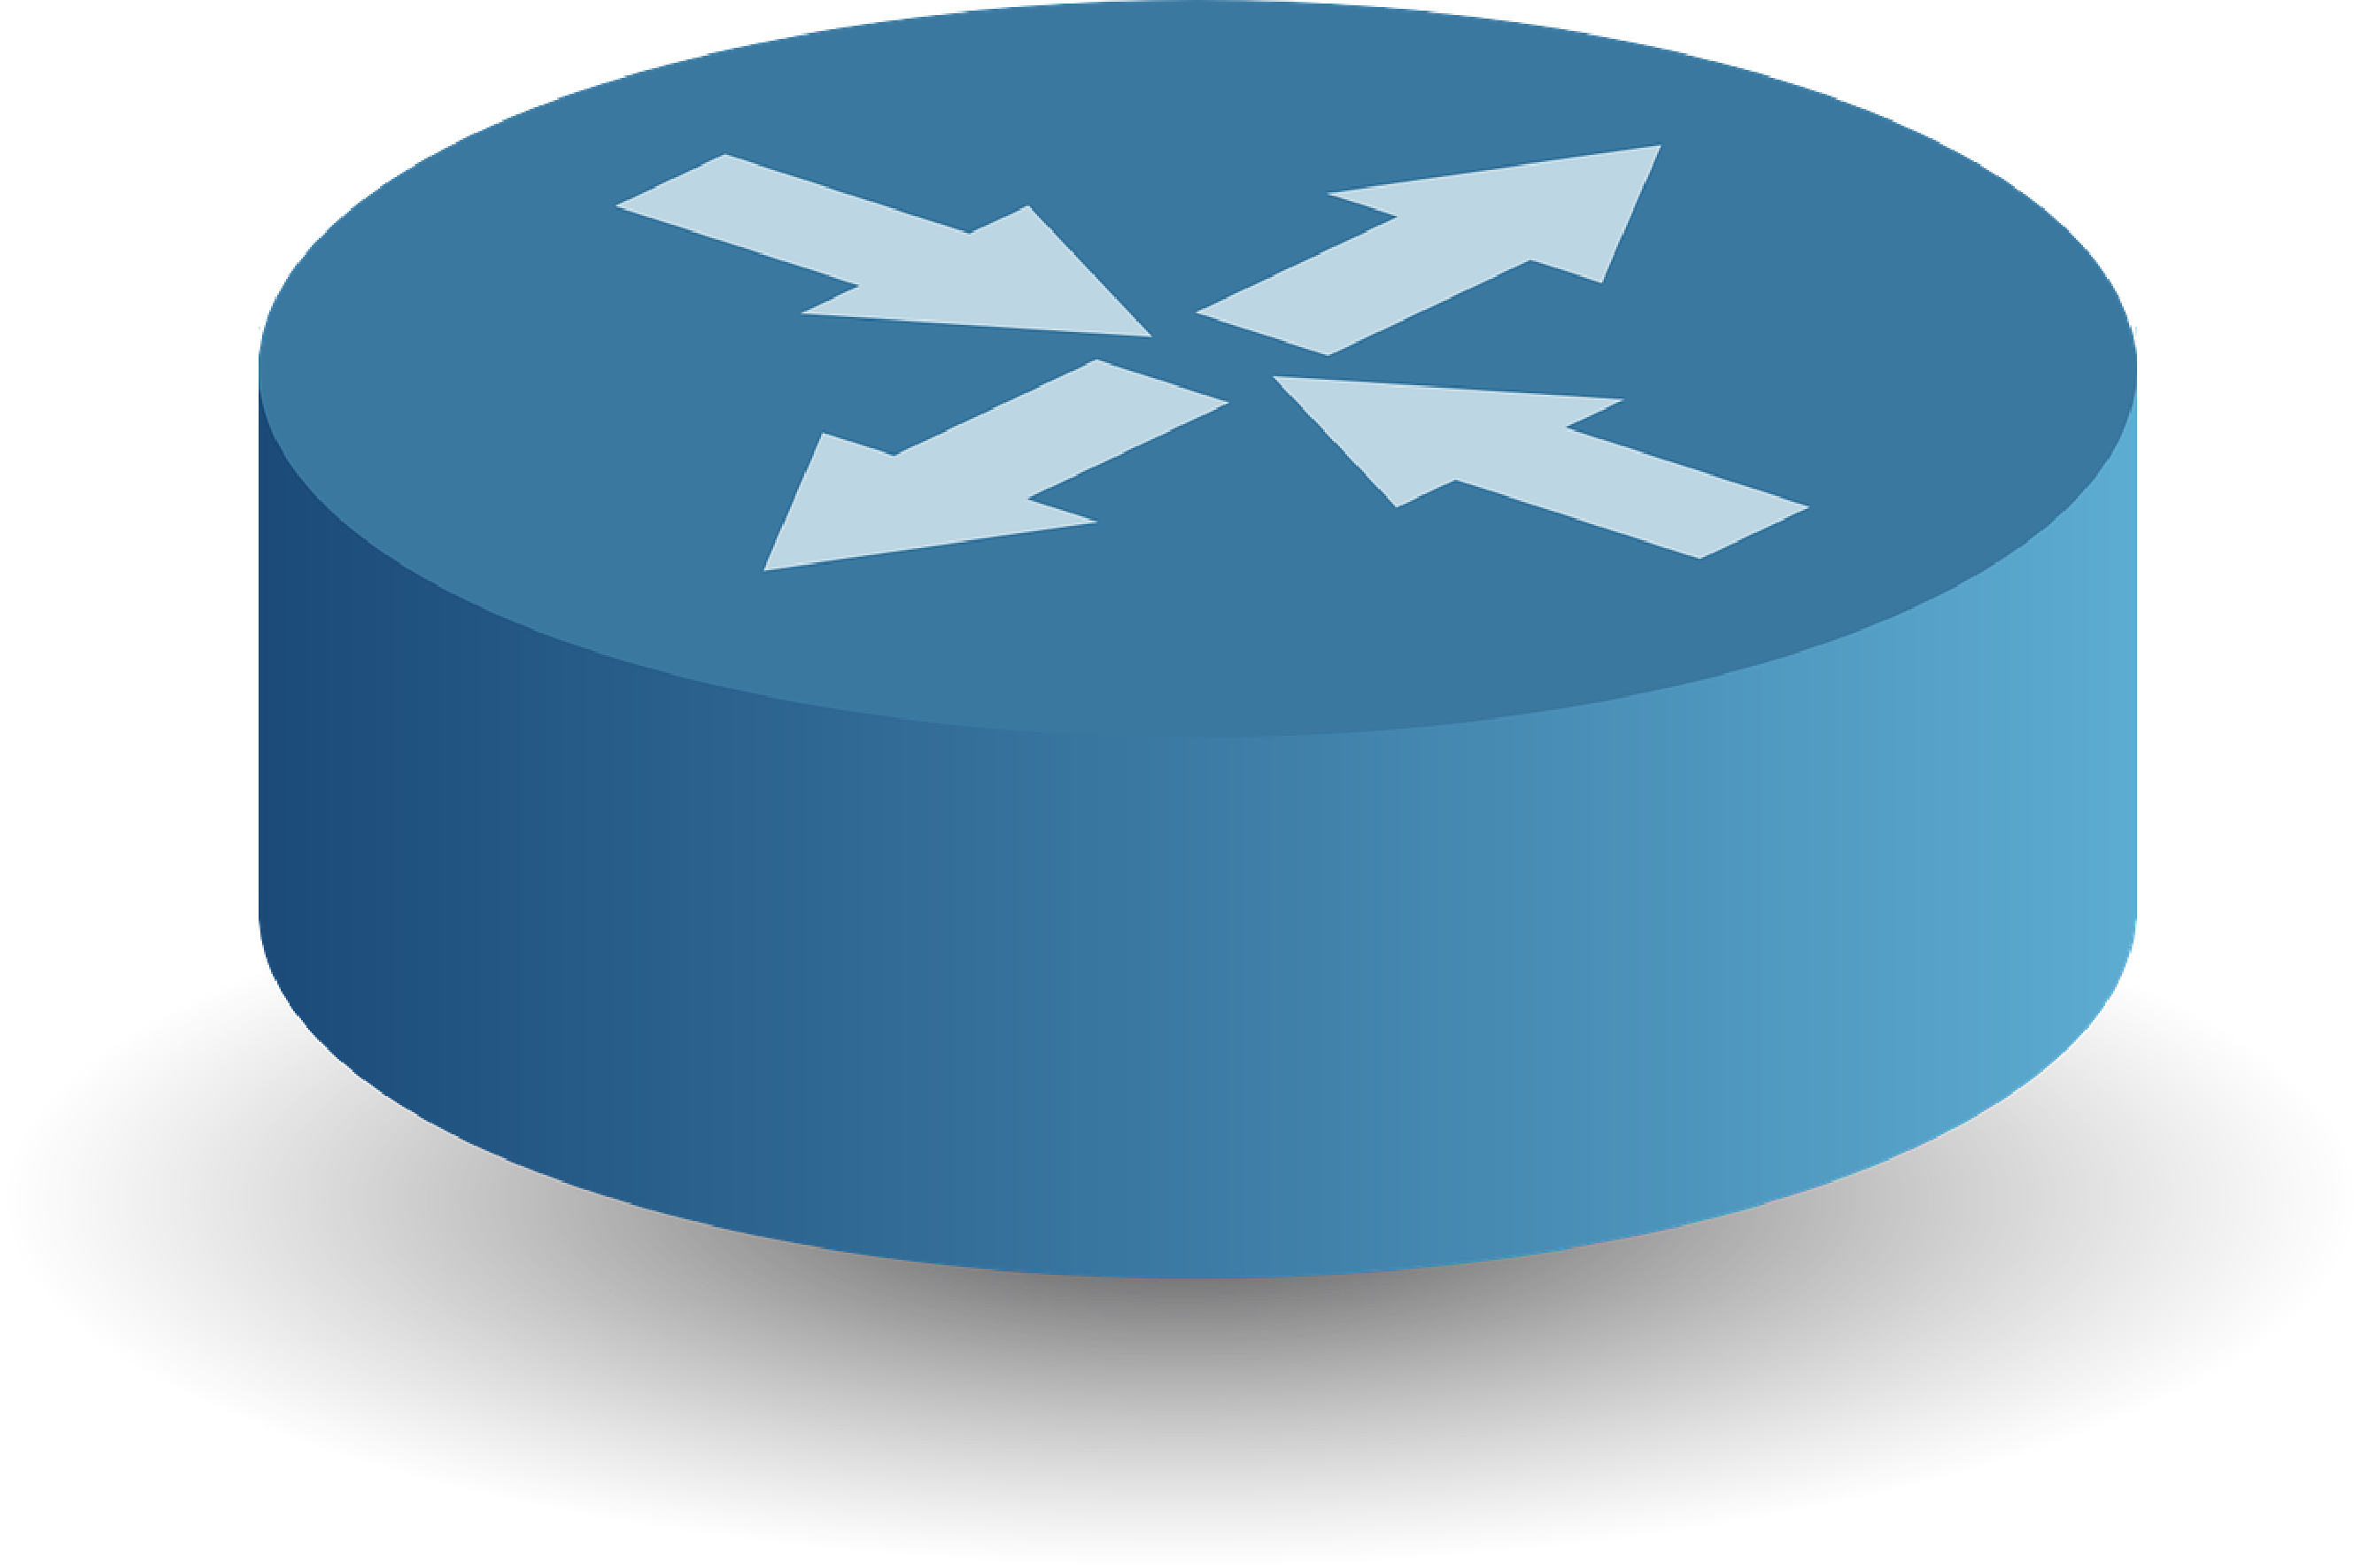
\includegraphics[width=52.5pt,height=52.5pt]{figures/router-29825_1280.pdf}};
%Image [id:dp4786061414756648] 
\draw (248,407.83) node  {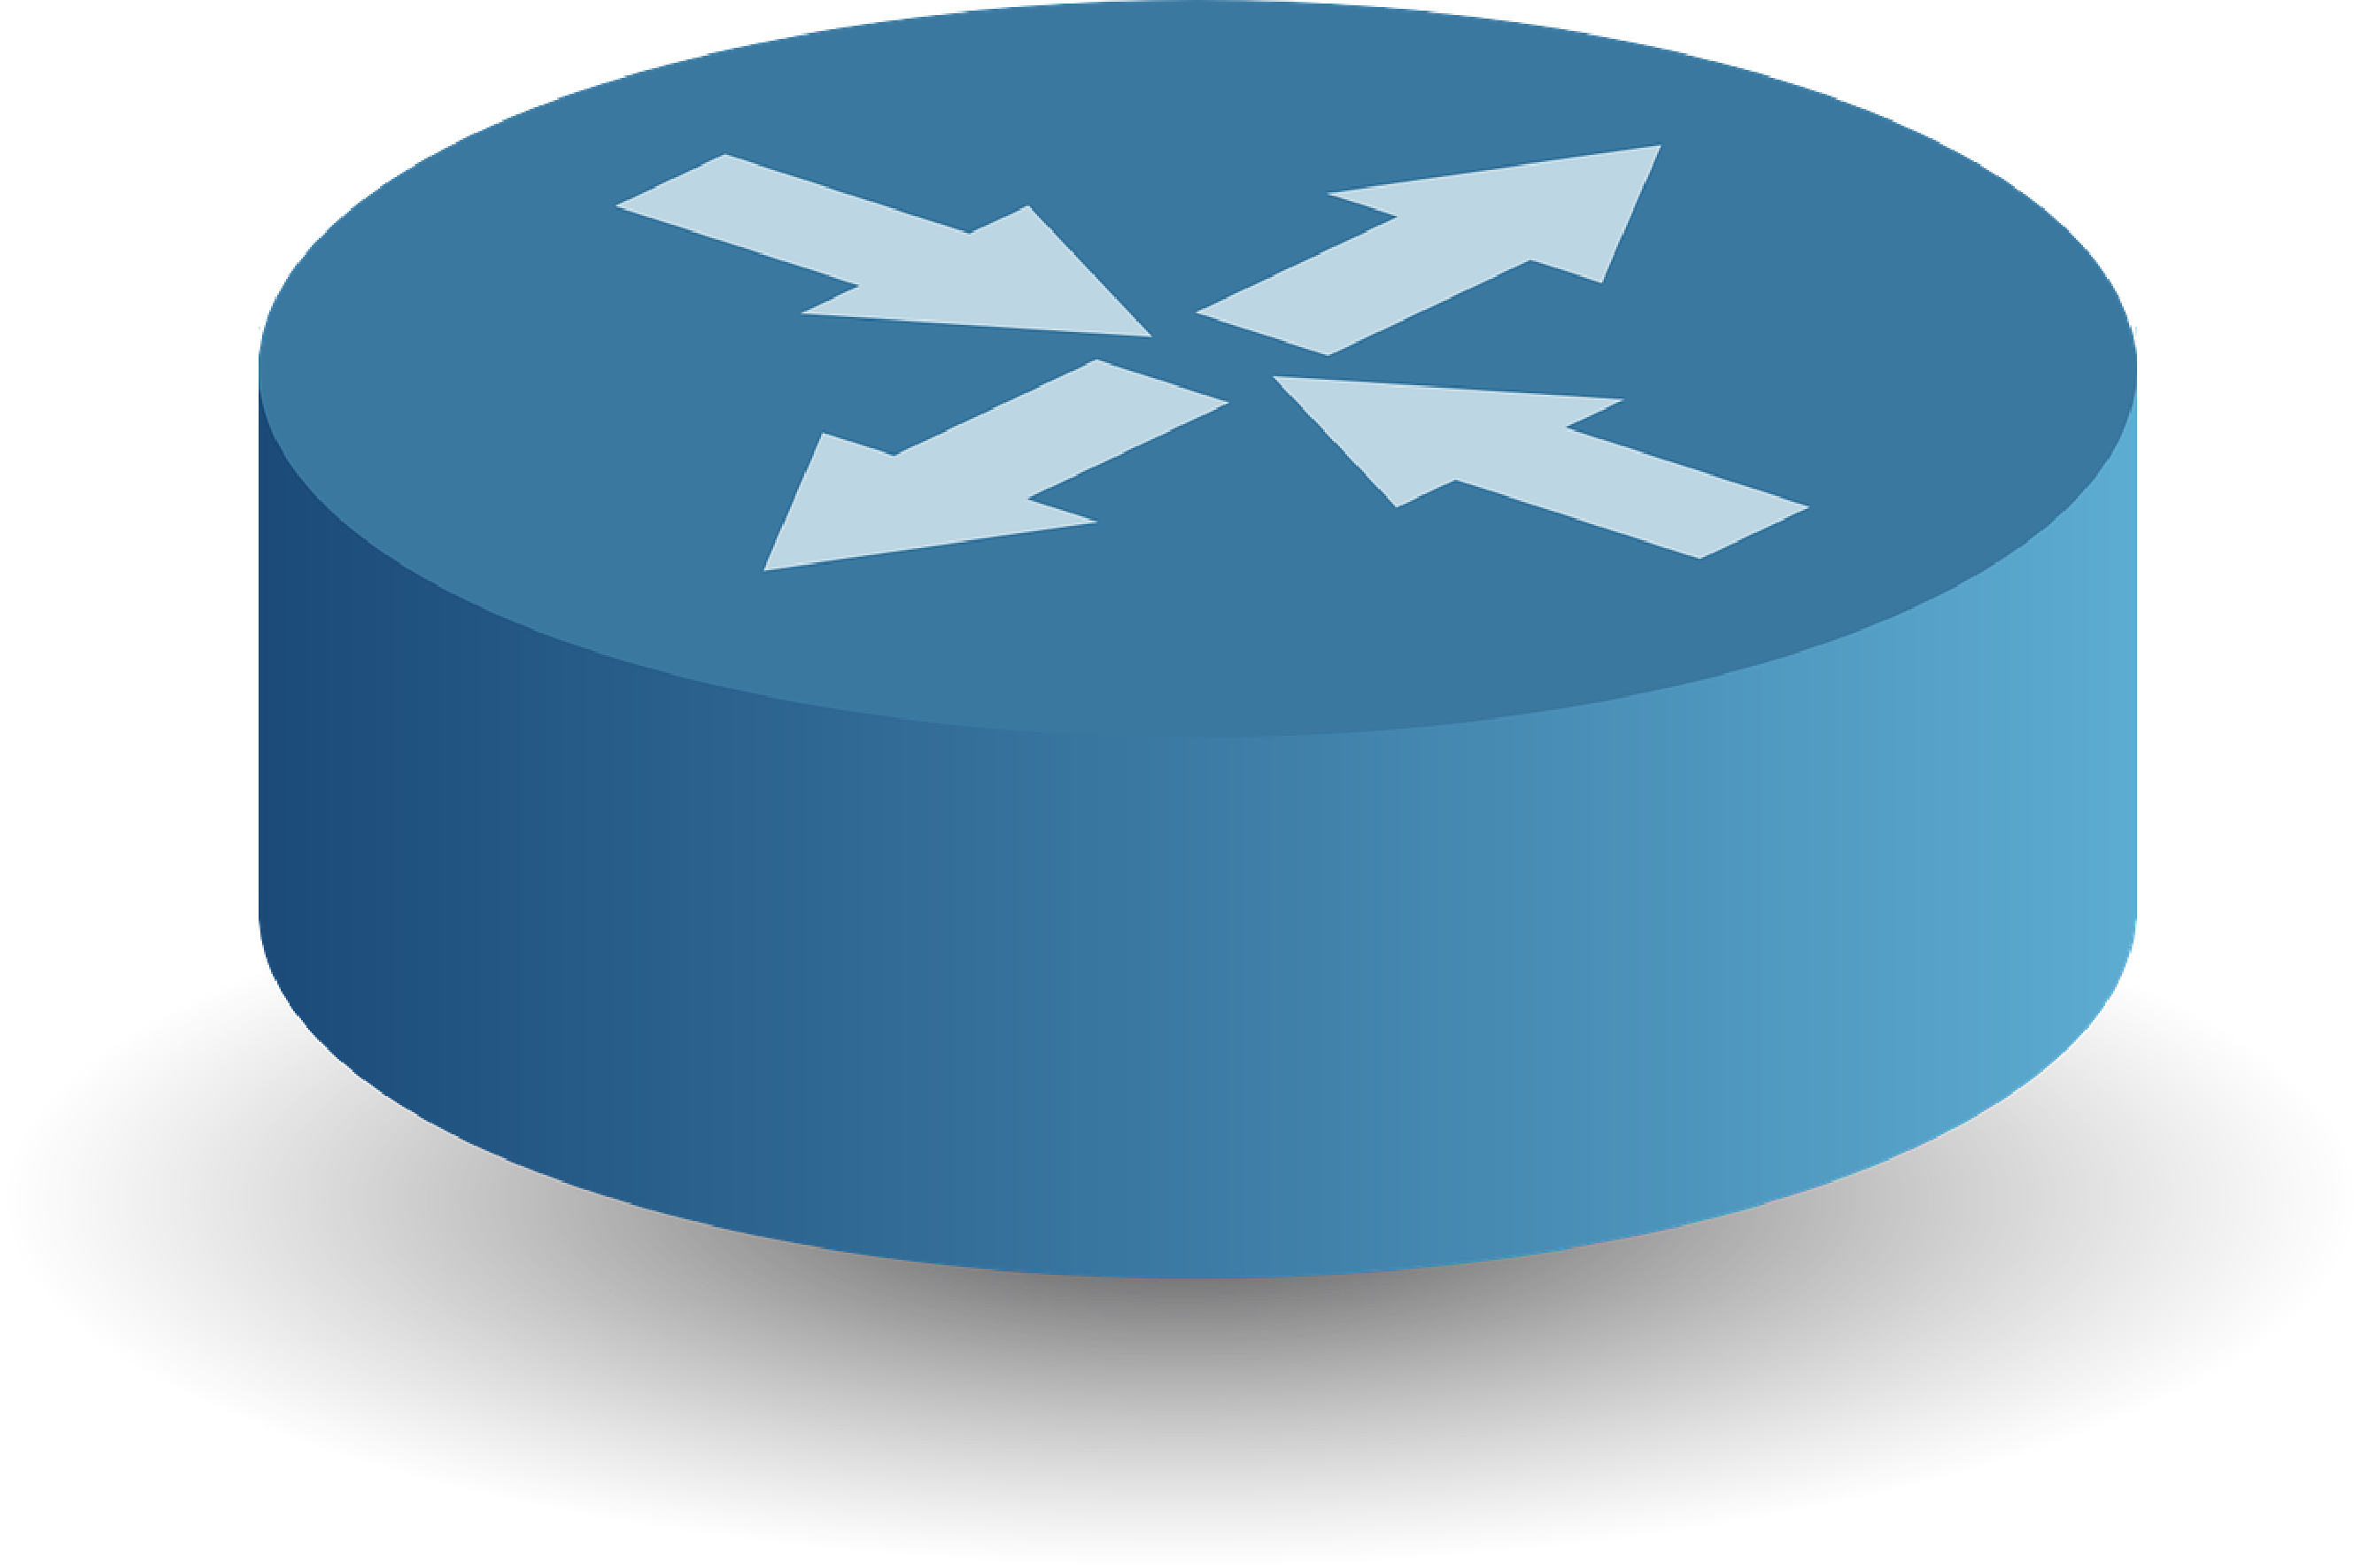
\includegraphics[width=52.5pt,height=52.5pt]{figures/router-29825_1280.pdf}};

%Image [id:dp9691436731399989] 
\draw (365.5,467.83) node  {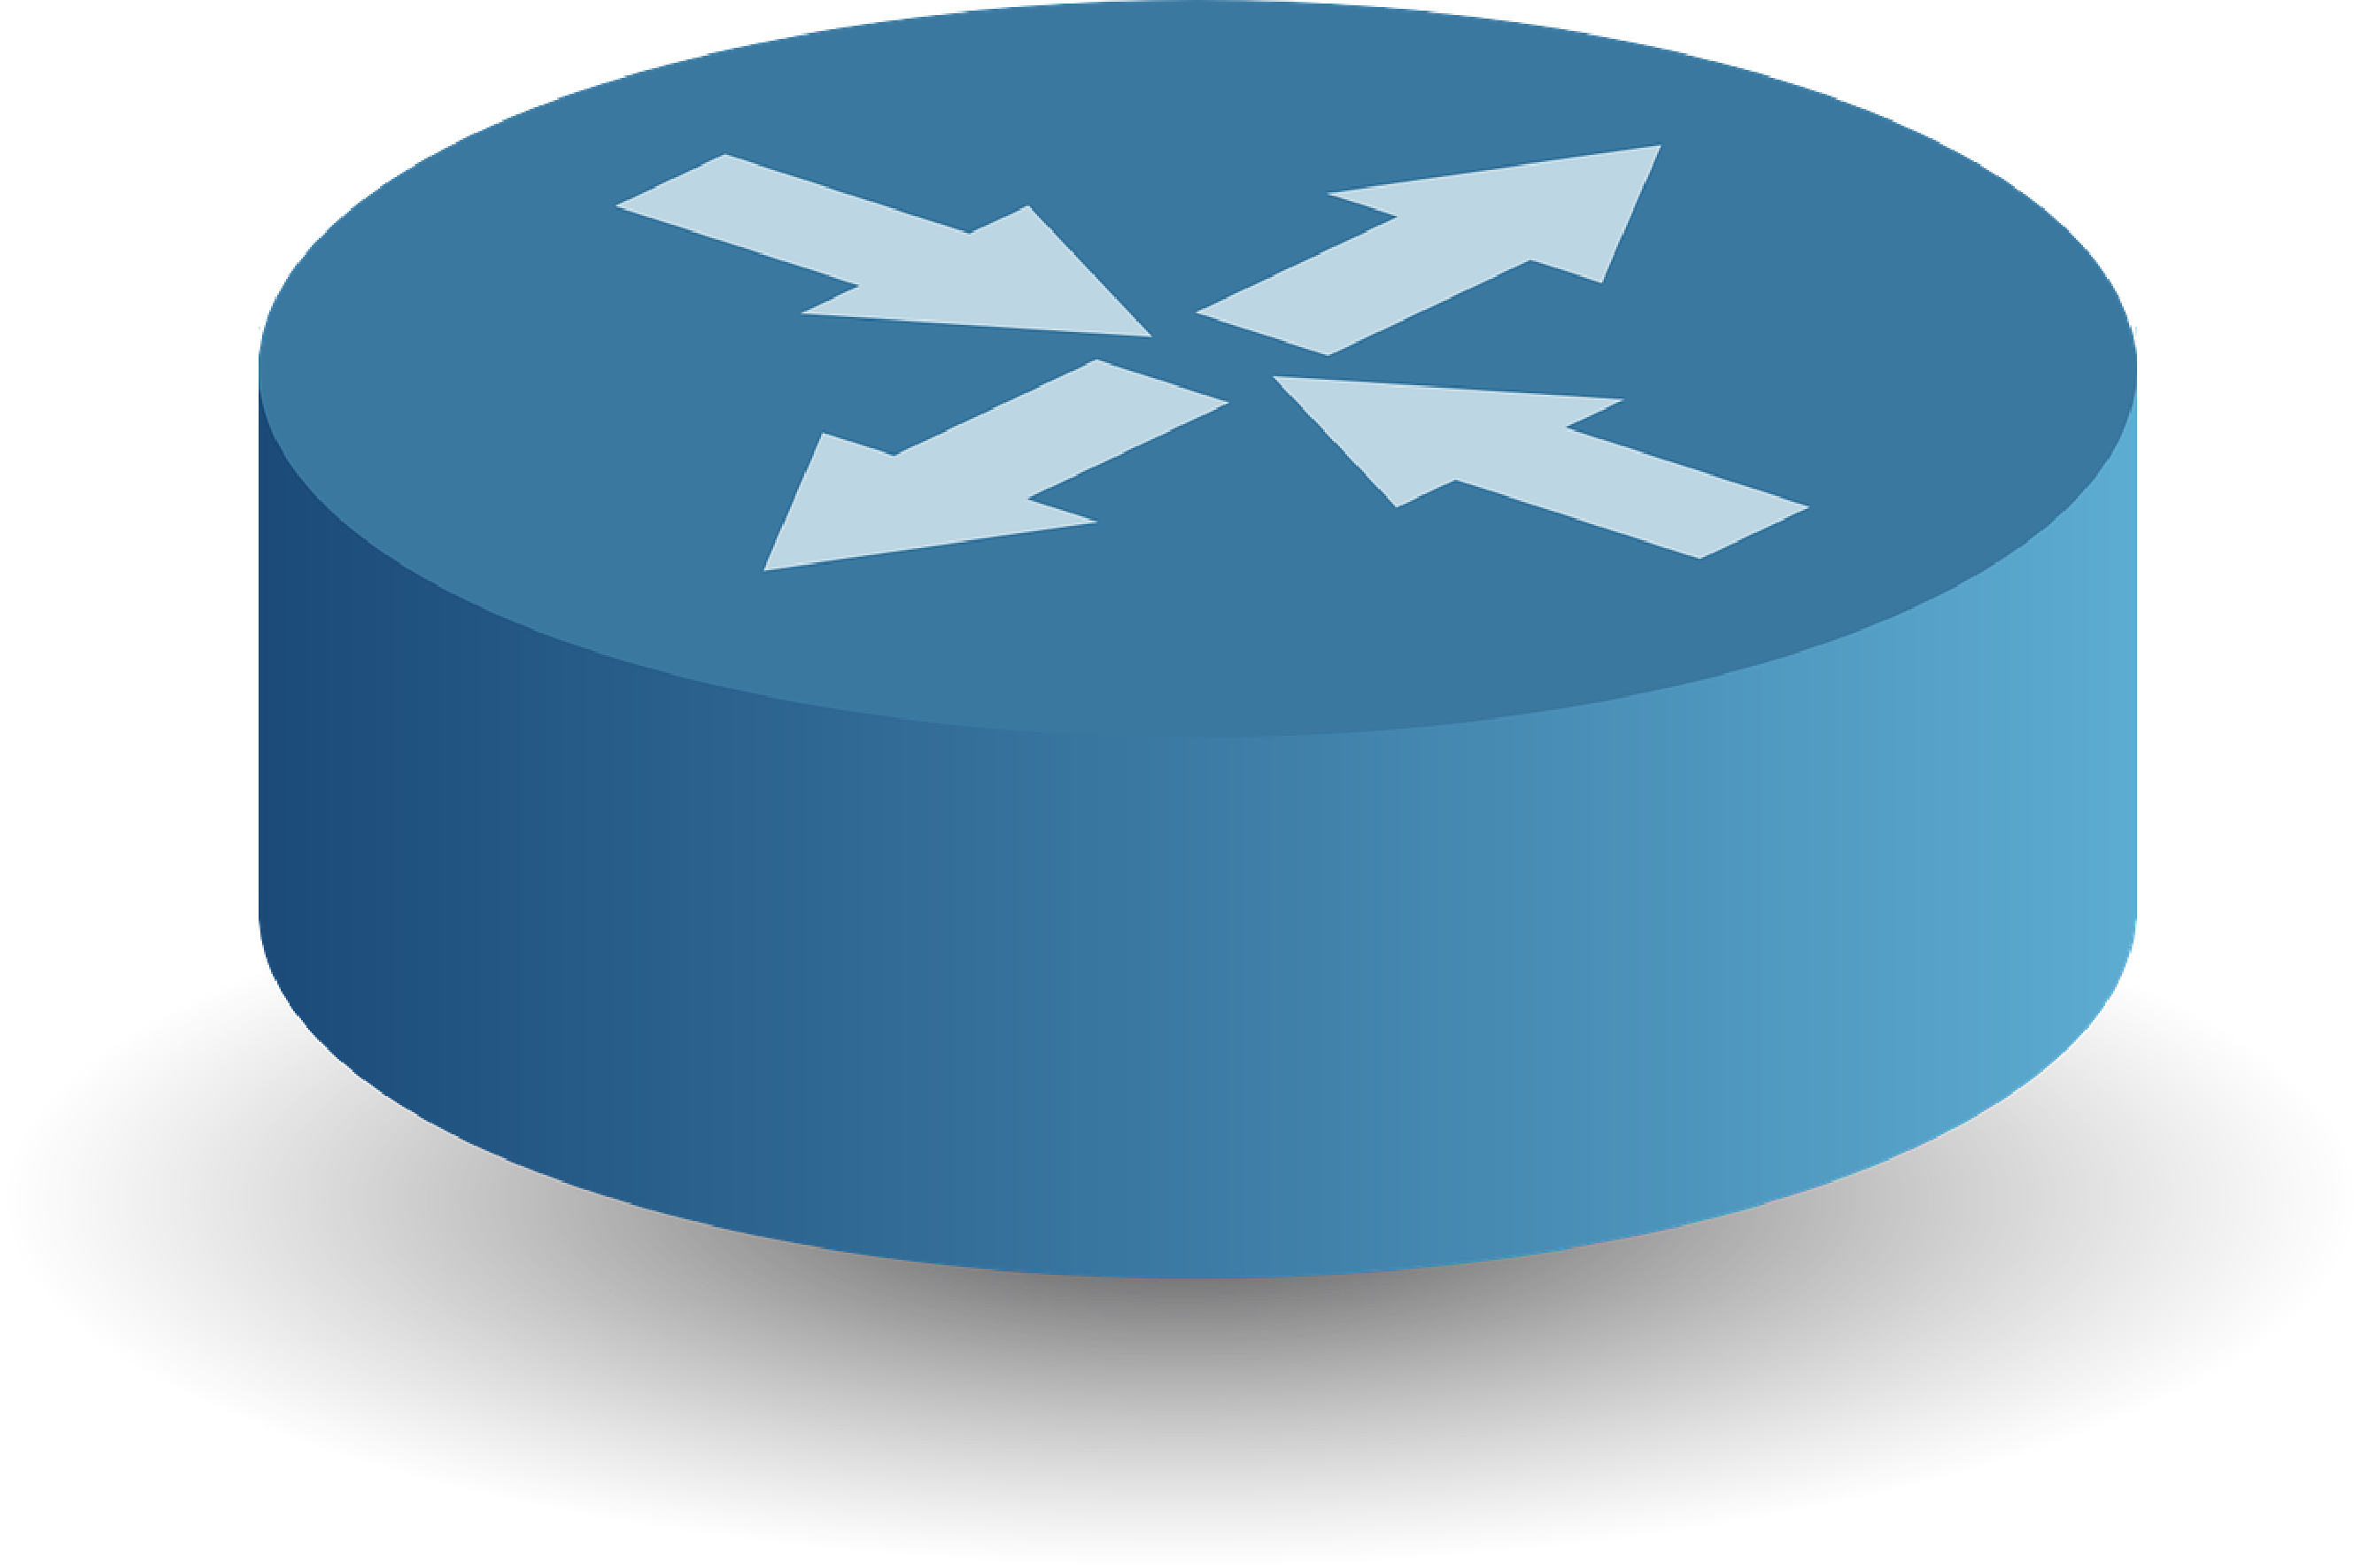
\includegraphics[width=52.5pt,height=52.5pt]{figures/router-29825_1280.pdf}};
%Image [id:dp9494715890151124] 
\draw (130.5,467.83) node  {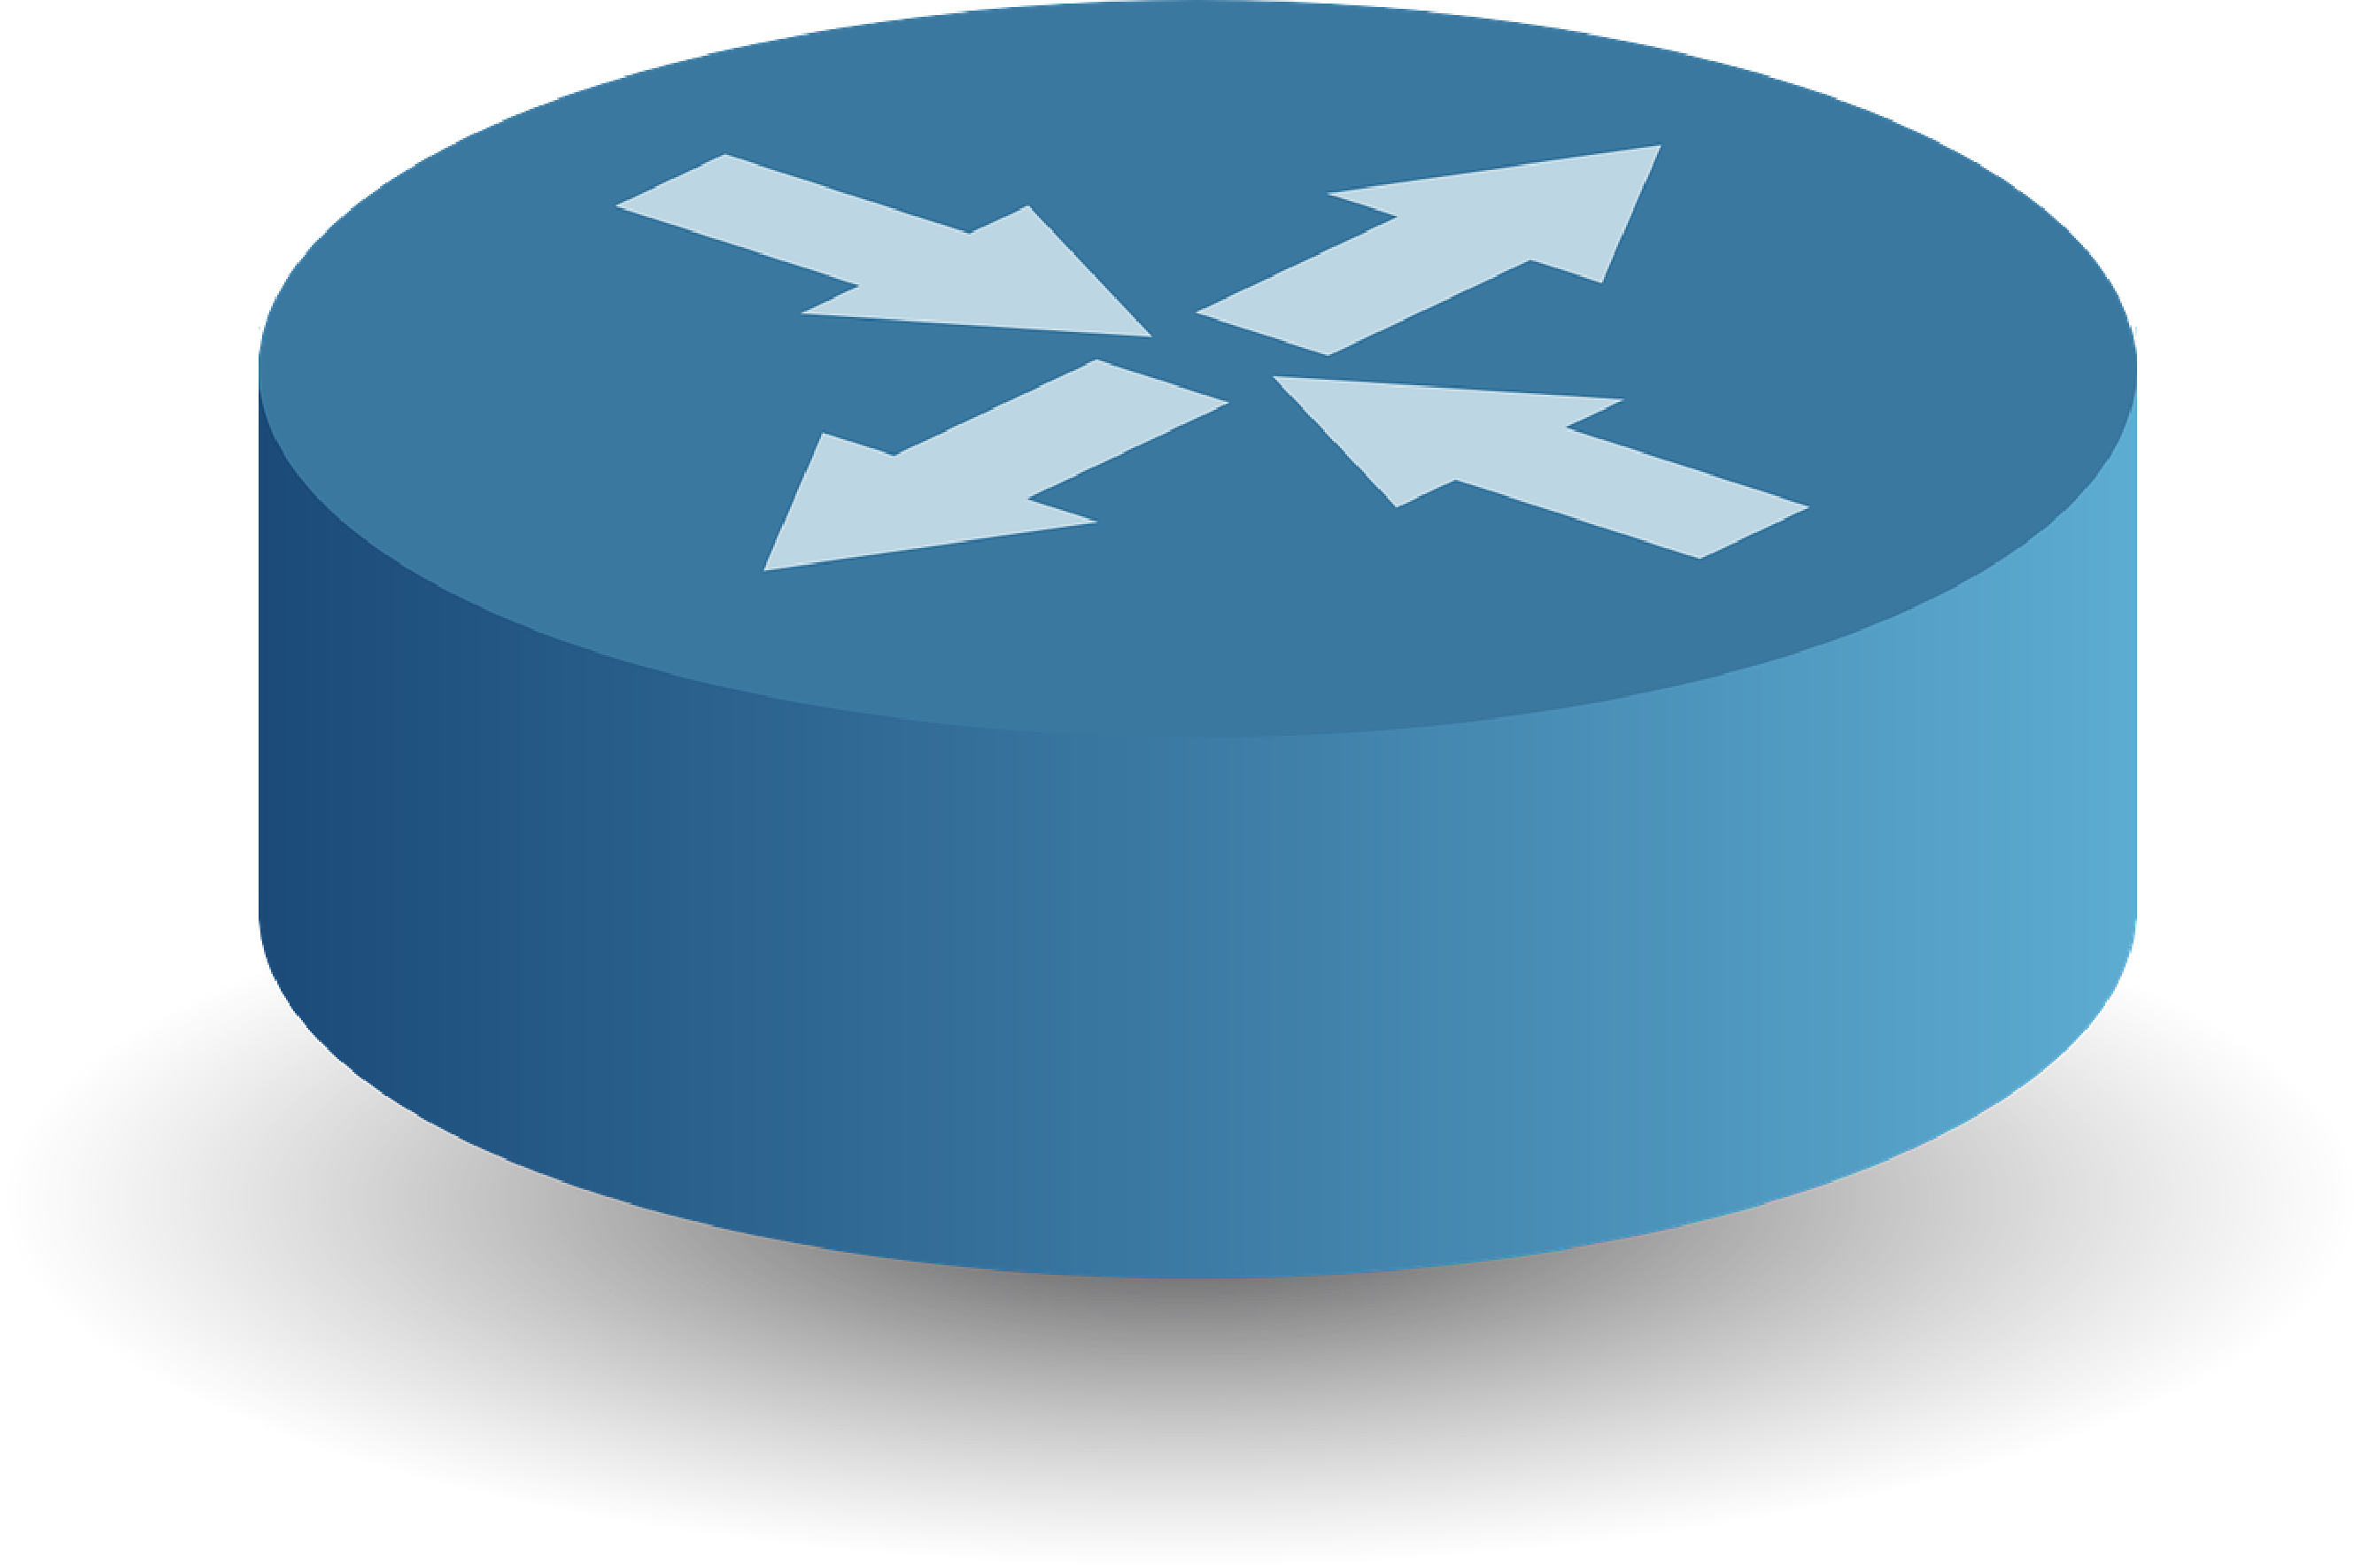
\includegraphics[width=52.5pt,height=52.5pt]{figures/router-29825_1280.pdf}};




%Rounded Rect [id:dp3362169615585995] 
\draw  [fill={rgb, 255:red, 246; green, 185; blue, 255 }  ,fill opacity=1 ] (14.33,161.8) .. controls (14.33,142.3) and (30.14,126.5) .. (49.63,126.5) -- (421.03,126.5) .. controls (440.53,126.5) and (456.33,142.3) .. (456.33,161.8) -- (456.33,267.7) .. controls (456.33,287.2) and (440.53,303) .. (421.03,303) -- (49.63,303) .. controls (30.14,303) and (14.33,287.2) .. (14.33,267.7) -- cycle ;
%Rounded Rect [id:dp9567502407138185] 
\draw  [fill={rgb, 255:red, 255; green, 255; blue, 255 }  ,fill opacity=1 ][line width=1.5]  (210.83,194.22) .. controls (210.83,190.83) and (213.58,188.08) .. (216.97,188.08) -- (310.7,188.08) .. controls (314.09,188.08) and (316.83,190.83) .. (316.83,194.22) -- (316.83,212.62) .. controls (316.83,216) and (314.09,218.75) .. (310.7,218.75) -- (216.97,218.75) .. controls (213.58,218.75) and (210.83,216) .. (210.83,212.62) -- cycle ;

%Rounded Rect [id:dp009214837373342832] 
\draw  [fill={rgb, 255:red, 255; green, 255; blue, 255 }  ,fill opacity=1 ][line width=1.5]  (51.46,194.22) .. controls (51.46,190.83) and (54.2,188.08) .. (57.59,188.08) -- (175.07,188.08) .. controls (178.46,188.08) and (181.21,190.83) .. (181.21,194.22) -- (181.21,212.62) .. controls (181.21,216) and (178.46,218.75) .. (175.07,218.75) -- (57.59,218.75) .. controls (54.2,218.75) and (51.46,216) .. (51.46,212.62) -- cycle ;

%Rounded Rect [id:dp7376385480360085] 
\draw  [fill={rgb, 255:red, 255; green, 255; blue, 255 }  ,fill opacity=1 ][line width=1.5]  (172.05,116.22) .. controls (172.05,112.83) and (174.79,110.08) .. (178.18,110.08) -- (349.49,110.08) .. controls (352.87,110.08) and (355.62,112.83) .. (355.62,116.22) -- (355.62,134.62) .. controls (355.62,138) and (352.87,140.75) .. (349.49,140.75) -- (178.18,140.75) .. controls (174.79,140.75) and (172.05,138) .. (172.05,134.62) -- cycle ;

%Rounded Rect [id:dp19791531901769066] 
\draw  [fill={rgb, 255:red, 255; green, 255; blue, 255 }  ,fill opacity=1 ][line width=1.5]  (172.05,294.22) .. controls (172.05,290.83) and (174.79,288.08) .. (178.18,288.08) -- (349.49,288.08) .. controls (352.87,288.08) and (355.62,290.83) .. (355.62,294.22) -- (355.62,312.62) .. controls (355.62,316) and (352.87,318.75) .. (349.49,318.75) -- (178.18,318.75) .. controls (174.79,318.75) and (172.05,316) .. (172.05,312.62) -- cycle ;

%Straight Lines [id:da3071607162532064] 
\draw  [dash pattern={on 4.5pt off 4.5pt}]  (262.56,144.33) -- (263.44,184.83) ;
\draw [shift={(263.5,187.83)}, rotate = 268.77] [fill={rgb, 255:red, 0; green, 0; blue, 0 }  ][line width=0.08]  [draw opacity=0] (10.72,-5.15) -- (0,0) -- (10.72,5.15) -- (7.12,0) -- cycle    ;
\draw [shift={(262.5,141.33)}, rotate = 88.77] [fill={rgb, 255:red, 0; green, 0; blue, 0 }  ][line width=0.08]  [draw opacity=0] (10.72,-5.15) -- (0,0) -- (10.72,5.15) -- (7.12,0) -- cycle    ;
%Straight Lines [id:da5811563165265446] 
\draw  [dash pattern={on 4.5pt off 4.5pt}]  (120.06,239.8) -- (119.14,220.83) ;
\draw [shift={(119,217.83)}, rotate = 447.25] [fill={rgb, 255:red, 0; green, 0; blue, 0 }  ][line width=0.08]  [draw opacity=0] (10.72,-5.15) -- (0,0) -- (10.72,5.15) -- (7.12,0) -- cycle    ;
\draw [shift={(120.2,242.8)}, rotate = 267.25] [fill={rgb, 255:red, 0; green, 0; blue, 0 }  ][line width=0.08]  [draw opacity=0] (10.72,-5.15) -- (0,0) -- (10.72,5.15) -- (7.12,0) -- cycle    ;
%Straight Lines [id:da36813314079504633] 
\draw  [dash pattern={on 4.5pt off 4.5pt}]  (189,250) -- (209.32,215.21) ;
\draw [shift={(210.83,212.62)}, rotate = 480.29] [fill={rgb, 255:red, 0; green, 0; blue, 0 }  ][line width=0.08]  [draw opacity=0] (10.72,-5.15) -- (0,0) -- (10.72,5.15) -- (7.12,0) -- cycle    ;

%Straight Lines [id:da7736079542900215] 
\draw  [dash pattern={on 4.5pt off 4.5pt}]  (263,222.83) -- (263,284.83) ;
\draw [shift={(263,287.83)}, rotate = 270] [fill={rgb, 255:red, 0; green, 0; blue, 0 }  ][line width=0.08]  [draw opacity=0] (10.72,-5.15) -- (0,0) -- (10.72,5.15) -- (7.12,0) -- cycle    ;
\draw [shift={(263,219.83)}, rotate = 90] [fill={rgb, 255:red, 0; green, 0; blue, 0 }  ][line width=0.08]  [draw opacity=0] (10.72,-5.15) -- (0,0) -- (10.72,5.15) -- (7.12,0) -- cycle    ;
%Straight Lines [id:da5692634255089728] 
\draw  [dash pattern={on 4.5pt off 4.5pt}]  (185,204.23) -- (207,203.44) ;
\draw [shift={(210,203.33)}, rotate = 537.95] [fill={rgb, 255:red, 0; green, 0; blue, 0 }  ][line width=0.08]  [draw opacity=0] (10.72,-5.15) -- (0,0) -- (10.72,5.15) -- (7.12,0) -- cycle    ;
\draw [shift={(182,204.33)}, rotate = 357.95] [fill={rgb, 255:red, 0; green, 0; blue, 0 }  ][line width=0.08]  [draw opacity=0] (10.72,-5.15) -- (0,0) -- (10.72,5.15) -- (7.12,0) -- cycle    ;
%Straight Lines [id:da11917773489604144] 
\draw  [dash pattern={on 4.5pt off 4.5pt}]  (195.8,259.02) -- (328.77,256.62) ;
\draw [shift={(331.77,256.57)}, rotate = 538.97] [fill={rgb, 255:red, 0; green, 0; blue, 0 }  ][line width=0.08]  [draw opacity=0] (10.72,-5.15) -- (0,0) -- (10.72,5.15) -- (7.12,0) -- cycle    ;

%Straight Lines [id:da7770404819607903] 
\draw  [dash pattern={on 4.5pt off 4.5pt}]  (262.81,322.31) -- (262.98,351.33) ;
\draw [shift={(263,354.33)}, rotate = 269.65999999999997] [fill={rgb, 255:red, 0; green, 0; blue, 0 }  ][line width=0.08]  [draw opacity=0] (10.72,-5.15) -- (0,0) -- (10.72,5.15) -- (7.12,0) -- cycle    ;
\draw [shift={(262.79,319.31)}, rotate = 89.66] [fill={rgb, 255:red, 0; green, 0; blue, 0 }  ][line width=0.08]  [draw opacity=0] (10.72,-5.15) -- (0,0) -- (10.72,5.15) -- (7.12,0) -- cycle    ;
%Straight Lines [id:da8379163771385384] 
\draw  [dash pattern={on 4.5pt off 4.5pt}]  (145.98,273.33) -- (145.46,349.78) ;
\draw [shift={(145.44,352.78)}, rotate = 270.39] [fill={rgb, 255:red, 0; green, 0; blue, 0 }  ][line width=0.08]  [draw opacity=0] (10.72,-5.15) -- (0,0) -- (10.72,5.15) -- (7.12,0) -- cycle    ;
\draw [shift={(146,270.33)}, rotate = 90.39] [fill={rgb, 255:red, 0; green, 0; blue, 0 }  ][line width=0.08]  [draw opacity=0] (10.72,-5.15) -- (0,0) -- (10.72,5.15) -- (7.12,0) -- cycle    ;
%Straight Lines [id:da7179548819350594] 
\draw  [dash pattern={on 4.5pt off 4.5pt}]  (263,72.33) -- (263,106.33) ;
\draw [shift={(263,109.33)}, rotate = 270] [fill={rgb, 255:red, 0; green, 0; blue, 0 }  ][line width=0.08]  [draw opacity=0] (10.72,-5.15) -- (0,0) -- (10.72,5.15) -- (7.12,0) -- cycle    ;
\draw [shift={(263,69.33)}, rotate = 90] [fill={rgb, 255:red, 0; green, 0; blue, 0 }  ][line width=0.08]  [draw opacity=0] (10.72,-5.15) -- (0,0) -- (10.72,5.15) -- (7.12,0) -- cycle    ;
%Rounded Rect [id:dp3518984914276363] 
\draw  [fill={rgb, 255:red, 56; green, 144; blue, 249 }  ,fill opacity=1 ] (121.5,17.37) .. controls (121.5,9.98) and (127.48,4) .. (134.87,4) -- (361.13,4) .. controls (368.52,4) and (374.5,9.98) .. (374.5,17.37) -- (374.5,57.47) .. controls (374.5,64.85) and (368.52,70.83) .. (361.13,70.83) -- (134.87,70.83) .. controls (127.48,70.83) and (121.5,64.85) .. (121.5,57.47) -- cycle ;
%Rounded Rect [id:dp09188382569915587] 
\draw  [color={rgb, 255:red, 0; green, 0; blue, 0 }  ,draw opacity=1 ][fill={rgb, 255:red, 255; green, 255; blue, 255 }  ,fill opacity=1 ][dash pattern={on 5.63pt off 4.5pt}][line width=1.5]  (129.7,35.2) .. controls (129.7,31.87) and (132.4,29.17) .. (135.73,29.17) -- (234.94,29.17) .. controls (238.27,29.17) and (240.97,31.87) .. (240.97,35.2) -- (240.97,53.3) .. controls (240.97,56.63) and (238.27,59.33) .. (234.94,59.33) -- (135.73,59.33) .. controls (132.4,59.33) and (129.7,56.63) .. (129.7,53.3) -- cycle ;
%Rounded Rect [id:dp24603064281963627] 
\draw  [color={rgb, 255:red, 0; green, 0; blue, 0 }  ,draw opacity=1 ][fill={rgb, 255:red, 255; green, 255; blue, 255 }  ,fill opacity=1 ][dash pattern={on 5.63pt off 4.5pt}][line width=1.5]  (255.03,35.2) .. controls (255.03,31.87) and (257.73,29.17) .. (261.06,29.17) -- (360.27,29.17) .. controls (363.6,29.17) and (366.3,31.87) .. (366.3,35.2) -- (366.3,53.3) .. controls (366.3,56.63) and (363.6,59.33) .. (360.27,59.33) -- (261.06,59.33) .. controls (257.73,59.33) and (255.03,56.63) .. (255.03,53.3) -- cycle ;

%Rounded Rect [id:dp758697930562836] 
\draw  [fill={rgb, 255:red, 255; green, 255; blue, 255 }  ,fill opacity=1 ][line width=1.5]  (109.06,245.55) .. controls (109.06,242.16) and (111.81,239.42) .. (115.19,239.42) -- (191.47,239.42) .. controls (194.86,239.42) and (197.6,242.16) .. (197.6,245.55) -- (197.6,263.95) .. controls (197.6,267.34) and (194.86,270.08) .. (191.47,270.08) -- (115.19,270.08) .. controls (111.81,270.08) and (109.06,267.34) .. (109.06,263.95) -- cycle ;

%Straight Lines [id:da6795518551939627] 
\draw  [dash pattern={on 4.5pt off 4.5pt}]  (325,143.83) -- (324.78,284.78) ;
\draw [shift={(324.78,287.78)}, rotate = 270.09000000000003] [fill={rgb, 255:red, 0; green, 0; blue, 0 }  ][line width=0.08]  [draw opacity=0] (10.72,-5.15) -- (0,0) -- (10.72,5.15) -- (7.12,0) -- cycle    ;
\draw [shift={(325,140.83)}, rotate = 90.09] [fill={rgb, 255:red, 0; green, 0; blue, 0 }  ][line width=0.08]  [draw opacity=0] (10.72,-5.15) -- (0,0) -- (10.72,5.15) -- (7.12,0) -- cycle    ;
%Straight Lines [id:da055910518428688105] 
\draw  [dash pattern={on 4.5pt off 4.5pt}]  (185.78,140.44) -- (185.72,236.92) ;
\draw [shift={(185.72,239.92)}, rotate = 270.03] [fill={rgb, 255:red, 0; green, 0; blue, 0 }  ][line width=0.08]  [draw opacity=0] (10.72,-5.15) -- (0,0) -- (10.72,5.15) -- (7.12,0) -- cycle    ;

%Straight Lines [id:da9613526114203358] 
\draw  [dash pattern={on 4.5pt off 4.5pt}]  (66.42,221.44) -- (65.78,295.78) -- (169.05,294.26) ;
\draw [shift={(172.05,294.22)}, rotate = 539.1600000000001] [fill={rgb, 255:red, 0; green, 0; blue, 0 }  ][line width=0.08]  [draw opacity=0] (10.72,-5.15) -- (0,0) -- (10.72,5.15) -- (7.12,0) -- cycle    ;
\draw [shift={(66.44,218.44)}, rotate = 90.49] [fill={rgb, 255:red, 0; green, 0; blue, 0 }  ][line width=0.08]  [draw opacity=0] (10.72,-5.15) -- (0,0) -- (10.72,5.15) -- (7.12,0) -- cycle    ;
%Straight Lines [id:da3742893196331808] 
\draw  [dash pattern={on 4.5pt off 4.5pt}]  (348.07,143.83) -- (350.1,234.17) ;
\draw [shift={(350.17,237.17)}, rotate = 268.71] [fill={rgb, 255:red, 0; green, 0; blue, 0 }  ][line width=0.08]  [draw opacity=0] (10.72,-5.15) -- (0,0) -- (10.72,5.15) -- (7.12,0) -- cycle    ;
\draw [shift={(348,140.83)}, rotate = 88.71] [fill={rgb, 255:red, 0; green, 0; blue, 0 }  ][line width=0.08]  [draw opacity=0] (10.72,-5.15) -- (0,0) -- (10.72,5.15) -- (7.12,0) -- cycle    ;
%Rounded Rect [id:dp9140860086605985] 
\draw  [fill={rgb, 255:red, 255; green, 255; blue, 255 }  ,fill opacity=1 ][line width=1.5]  (335.83,245.55) .. controls (335.83,242.16) and (338.58,239.42) .. (341.97,239.42) -- (435.7,239.42) .. controls (439.09,239.42) and (441.83,242.16) .. (441.83,245.55) -- (441.83,263.95) .. controls (441.83,267.34) and (439.09,270.08) .. (435.7,270.08) -- (341.97,270.08) .. controls (338.58,270.08) and (335.83,267.34) .. (335.83,263.95) -- cycle ;

%Shape: Ellipse [id:dp3554083551130477] 
\draw  [color={rgb, 255:red, 208; green, 2; blue, 27 }  ,draw opacity=1 ] (188.3,153.75) .. controls (188.3,149.91) and (191.71,146.8) .. (195.93,146.8) .. controls (200.14,146.8) and (203.55,149.91) .. (203.55,153.75) .. controls (203.55,157.59) and (200.14,160.7) .. (195.93,160.7) .. controls (191.71,160.7) and (188.3,157.59) .. (188.3,153.75) -- cycle ;
%Shape: Ellipse [id:dp4084549692042517] 
\draw  [color={rgb, 255:red, 208; green, 2; blue, 27 }  ,draw opacity=1 ] (267.05,87.25) .. controls (267.05,83.41) and (270.46,80.3) .. (274.68,80.3) .. controls (278.89,80.3) and (282.3,83.41) .. (282.3,87.25) .. controls (282.3,91.09) and (278.89,94.2) .. (274.68,94.2) .. controls (270.46,94.2) and (267.05,91.09) .. (267.05,87.25) -- cycle ;
%Shape: Ellipse [id:dp6652927550013479] 
\draw  [color={rgb, 255:red, 208; green, 2; blue, 27 }  ,draw opacity=1 ] (264.8,156.5) .. controls (264.8,152.66) and (268.21,149.55) .. (272.43,149.55) .. controls (276.64,149.55) and (280.05,152.66) .. (280.05,156.5) .. controls (280.05,160.34) and (276.64,163.45) .. (272.43,163.45) .. controls (268.21,163.45) and (264.8,160.34) .. (264.8,156.5) -- cycle ;
%Shape: Ellipse [id:dp20966000134493123] 
\draw  [color={rgb, 255:red, 208; green, 2; blue, 27 }  ,draw opacity=1 ] (307.55,151.25) .. controls (307.55,147.41) and (310.96,144.3) .. (315.18,144.3) .. controls (319.39,144.3) and (322.8,147.41) .. (322.8,151.25) .. controls (322.8,155.09) and (319.39,158.2) .. (315.18,158.2) .. controls (310.96,158.2) and (307.55,155.09) .. (307.55,151.25) -- cycle ;
%Shape: Ellipse [id:dp0540432112177649] 
\draw  [color={rgb, 255:red, 208; green, 2; blue, 27 }  ,draw opacity=1 ] (355.55,180.75) .. controls (355.55,176.91) and (358.96,173.8) .. (363.18,173.8) .. controls (367.39,173.8) and (370.8,176.91) .. (370.8,180.75) .. controls (370.8,184.59) and (367.39,187.7) .. (363.18,187.7) .. controls (358.96,187.7) and (355.55,184.59) .. (355.55,180.75) -- cycle ;
%Shape: Ellipse [id:dp45917488569940357] 
\draw  [color={rgb, 255:red, 208; green, 2; blue, 27 }  ,draw opacity=1 ] (185.3,189.34) .. controls (185.3,185.5) and (188.71,182.39) .. (192.93,182.39) .. controls (197.14,182.39) and (200.55,185.5) .. (200.55,189.34) .. controls (200.55,193.17) and (197.14,196.28) .. (192.93,196.28) .. controls (188.71,196.28) and (185.3,193.17) .. (185.3,189.34) -- cycle ;

%Shape: Ellipse [id:dp5545246337247209] 
\draw  [color={rgb, 255:red, 208; green, 2; blue, 27 }  ,draw opacity=1 ] (199.3,229) .. controls (199.3,225.16) and (202.71,222.05) .. (206.93,222.05) .. controls (211.14,222.05) and (214.55,225.16) .. (214.55,229) .. controls (214.55,232.84) and (211.14,235.95) .. (206.93,235.95) .. controls (202.71,235.95) and (199.3,232.84) .. (199.3,229) -- cycle ;
%Shape: Ellipse [id:dp4152293630769399] 
\draw  [color={rgb, 255:red, 208; green, 2; blue, 27 }  ,draw opacity=1 ] (264.1,229.6) .. controls (264.1,225.76) and (267.51,222.65) .. (271.73,222.65) .. controls (275.94,222.65) and (279.35,225.76) .. (279.35,229.6) .. controls (279.35,233.44) and (275.94,236.55) .. (271.73,236.55) .. controls (267.51,236.55) and (264.1,233.44) .. (264.1,229.6) -- cycle ;
%Shape: Ellipse [id:dp7028700683432993] 
\draw  [color={rgb, 255:red, 208; green, 2; blue, 27 }  ,draw opacity=1 ] (230.1,249.27) .. controls (230.1,245.43) and (233.51,242.32) .. (237.73,242.32) .. controls (241.94,242.32) and (245.35,245.43) .. (245.35,249.27) .. controls (245.35,253.11) and (241.94,256.22) .. (237.73,256.22) .. controls (233.51,256.22) and (230.1,253.11) .. (230.1,249.27) -- cycle ;
%Shape: Ellipse [id:dp07410075663096749] 
\draw  [color={rgb, 255:red, 208; green, 2; blue, 27 }  ,draw opacity=1 ] (121.1,228.62) .. controls (121.1,224.05) and (125.15,220.35) .. (130.15,220.35) .. controls (135.15,220.35) and (139.2,224.05) .. (139.2,228.62) .. controls (139.2,233.18) and (135.15,236.88) .. (130.15,236.88) .. controls (125.15,236.88) and (121.1,233.18) .. (121.1,228.62) -- cycle ;
%Shape: Ellipse [id:dp30224928873301715] 
\draw  [color={rgb, 255:red, 208; green, 2; blue, 27 }  ,draw opacity=1 ] (68.3,284.22) .. controls (68.3,279.65) and (72.35,275.95) .. (77.35,275.95) .. controls (82.35,275.95) and (86.4,279.65) .. (86.4,284.22) .. controls (86.4,288.78) and (82.35,292.48) .. (77.35,292.48) .. controls (72.35,292.48) and (68.3,288.78) .. (68.3,284.22) -- cycle ;
%Shape: Ellipse [id:dp3894329820493001] 
\draw  [color={rgb, 255:red, 208; green, 2; blue, 27 }  ,draw opacity=1 ] (149.5,280.62) .. controls (149.5,276.05) and (153.55,272.35) .. (158.55,272.35) .. controls (163.55,272.35) and (167.6,276.05) .. (167.6,280.62) .. controls (167.6,285.18) and (163.55,288.88) .. (158.55,288.88) .. controls (153.55,288.88) and (149.5,285.18) .. (149.5,280.62) -- cycle ;
%Shape: Ellipse [id:dp8973642196115625] 
\draw  [color={rgb, 255:red, 208; green, 2; blue, 27 }  ,draw opacity=1 ] (375.5,281.22) .. controls (375.5,276.65) and (379.55,272.95) .. (384.55,272.95) .. controls (389.55,272.95) and (393.6,276.65) .. (393.6,281.22) .. controls (393.6,285.78) and (389.55,289.48) .. (384.55,289.48) .. controls (379.55,289.48) and (375.5,285.78) .. (375.5,281.22) -- cycle ;
%Shape: Ellipse [id:dp6431628695495194] 
\draw  [color={rgb, 255:red, 208; green, 2; blue, 27 }  ,draw opacity=1 ] (265.5,335.02) .. controls (265.5,330.45) and (269.55,326.75) .. (274.55,326.75) .. controls (279.55,326.75) and (283.6,330.45) .. (283.6,335.02) .. controls (283.6,339.58) and (279.55,343.28) .. (274.55,343.28) .. controls (269.55,343.28) and (265.5,339.58) .. (265.5,335.02) -- cycle ;
%Straight Lines [id:da6717664493405898] 
\draw  [dash pattern={on 4.5pt off 4.5pt}]  (404.17,275.17) -- (404.17,293.17) -- (355.62,294.22) ;

\draw [shift={(404.17,272.17)}, rotate = 90] [fill={rgb, 255:red, 0; green, 0; blue, 0 }  ][line width=0.08]  [draw opacity=0] (10.72,-5.15) -- (0,0) -- (10.72,5.15) -- (7.12,0) -- cycle    ;

% Text Node
\draw (106.66,137.09) node  [font=\small] [align=left] {Network Hypervisor};
% Text Node
\draw (196.26,154.45) node  [color={rgb, 255:red, 208; green, 2; blue, 27 }  ,opacity=1 ] [align=left] {3};
% Text Node
\draw (275.01,86.95) node  [color={rgb, 255:red, 208; green, 2; blue, 27 }  ,opacity=1 ] [align=left] {1};
% Text Node
\draw (272.76,157.2) node  [font=\small,color={rgb, 255:red, 208; green, 2; blue, 27 }  ,opacity=1 ] [align=left] {2};
% Text Node
\draw (314.51,151.95) node  [font=\small,color={rgb, 255:red, 208; green, 2; blue, 27 }  ,opacity=1 ] [align=left] {4};
% Text Node
\draw (364.55,180.75) node  [font=\small,color={rgb, 255:red, 208; green, 2; blue, 27 }  ,opacity=1 ] [align=left] {5};
% Text Node
\draw (207.26,228.7) node  [font=\small,color={rgb, 255:red, 208; green, 2; blue, 27 }  ,opacity=1 ] [align=left] {7};
% Text Node
\draw (272.06,229.3) node  [font=\small,color={rgb, 255:red, 208; green, 2; blue, 27 }  ,opacity=1 ] [align=left] {8};
% Text Node
\draw (238.06,248.97) node  [font=\small,color={rgb, 255:red, 208; green, 2; blue, 27 }  ,opacity=1 ] [align=left] {9};
% Text Node
\draw (130.15,228.62) node  [font=\small,color={rgb, 255:red, 208; green, 2; blue, 27 }  ,opacity=1 ] [align=left] {{\small 10}};
% Text Node
\draw (77.35,284.22) node  [color={rgb, 255:red, 208; green, 2; blue, 27 }  ,opacity=1 ] [align=left] {{\small 11}};
% Text Node
\draw (157.55,280.62) node  [font=\small,color={rgb, 255:red, 208; green, 2; blue, 27 }  ,opacity=1 ] [align=left] {{\small 12}};
% Text Node
\draw (383.55,279.22) node  [color={rgb, 255:red, 208; green, 2; blue, 27 }  ,opacity=1 ] [align=left] {{\small 13}};
% Text Node
\draw (274.15,334.62) node  [color={rgb, 255:red, 208; green, 2; blue, 27 }  ,opacity=1 ] [align=left] {{\small 14}};
% Text Node
\draw (192.76,189.03) node  [color={rgb, 255:red, 208; green, 2; blue, 27 }  ,opacity=1 ] [align=left] {6};
% Text Node
\draw (388.83,256.08) node   [align=left] {Security};
% Text Node
\draw (153.33,256.08) node   [align=left] {Monitoring};
% Text Node
\draw (160.93,11.75) node  [font=\small,color={rgb, 255:red, 0; green, 0; blue, 0 }  ,opacity=1 ] [align=left] {Tenants};
% Text Node
\draw (310.08,45.17) node   [align=left] {\textcolor[rgb]{0,0,0}{Controllers}};
% Text Node
\draw (184.75,45.17) node   [align=left] {\textcolor[rgb]{0,0,0}{Applications}};
% Text Node
\draw (263.83,304.75) node   [align=left] {Data Plane Abstraction};
% Text Node
\draw (263.83,126.75) node   [align=left] {Control Plane Abstraction};
% Text Node
\draw (116.33,204.75) node   [align=left] {Resource Isolator};
% Text Node
\draw (263.83,204.75) node   [align=left] {VN Embedding};
% Text Node
\draw (143.66,363.17) node  [font=\small] [align=left] {Physical Infrastructure};


\end{tikzpicture}

\caption{Reference architecture of a network hypervisor}
\label{fig:reference-archi-nh}
\end{figure}
  
Figure~\ref{fig:reference-archi-nh} presents the reference architecture of a network hypervisor supporting a secure Virtual Network migration.
On a top-down perspective, there are three different levels in the virtualization architecture.
The tenant level, where end-users can deploy their own applications and SDN controllers, and interact with their Virtual Network.
The hypervisor level, including all the components required to achieve network virtualization, present the tenant with an abstract view, and interact with the physical infrastructure.
The lowest level includes all the networking equipments, like SDN-enabled switches and routers.

\subsubsection{Control Plane Abstraction}
The Control Plane Abstraction component (CPAC) provides the tenants with an interface to interact with the rest of the virtualization layer.
This component is an essential function for network virtualization and is implemented in every hypervisor.
When a tenant requests a Virtual Network, he describes his requirements in terms of virtual nodes, links, minimal bandwidth, security, \etc This request is received by the CPAC that transmits it to the VN Embedding component for further treatment.
The CPAC also defines tenants' capacities to interact with their Virtual Network, which can be either API-based control or full control.

API-based control limits the capacities of the tenants by only exposing an API to interact with their slice in a specific manner. For instance, the tenant may only use the API of the hypervisor or must use a specific programming language to implement his applications for the hypervisor~\cite{CompositionalHypervisor-Jin2014,NetworkHypervisor-Huang2013}. 
The full control describes an hypervisor where the tenant can use its\GB{``his''?} own application or SDN controller to interact with his Virtual Network. This solution is implemented by either slicing the infrastructure or maintaining a mapping between virtual and physical resources, as presented in the Section~\ref{sec:basic_def}.



\subsubsection{Data Plane Abstraction}
\label{sec:abstraction_comp}
The Data Plane Abstraction Component (DPAC) abstracts the physical infrastructure to serve each tenant with their own topology and resources.
This component is also an essential function of network virtualization and is implemented in every existing hypervisor.
It maintains the mapping between logical and physical topologies to translate logical decisions into physical ones.
% \GB{poor expression: the below paragraph should be rewritten}
It also makes sure that a tenant's operations on his Virtual Network does not interfere with the other tenants (\ie it maintains isolation between tenants). When a tenant deploys a new configuration in his network, such as routing protocols or ACLs, the DPAC is in charge of translating the virtual parameters and values used by the tenant into the corresponding ones for the physical infrastructure.

In practice, the abstraction is performed for several resources:

\subparagraph{\textbf{Topology}}\textbf{}\\
The hypervisor decouples the logical topology required by the tenant from the physical infrastructure.
Topology mapping can be either 1-to-1 or 1-to-many. 
The \textsl{1-to-1} mapping corresponds to the case where one virtual node (resp. link) is embedded in one physical node (resp. link), similarly to FlowVisor~\cite{FlowVisor-Sherwood2009} where the physical infrastructure is sliced and a small portion of it is presented to each tenant.
The \textsl{1-to-many} embeds a single virtual node or link to multiple physical resources, as presented in~\cite{OpenVirteX-Al-Shabibi2014,VeRTIGO-Corin2012a}.
A particular approach is when the tenant only requires one virtual node to interconnect his VMs, and does not want to bear the burden of maintaining the configuration of each underlying node. In the literature, this approach is referred to as the ``Big Switch Abstraction".


\subparagraph{\textbf{Flowspace}}\textbf{}\\
% \GB{below sentence is too long: to be rewriten}
The flowspace of a Virtual Network defines which header fields and the range of values in the flowspace that a tenant can use in his addressing and routing schemes. This includes MAC addresses, IP addresses, transport layer ports, VLAN IDs, \etc
FlowVisor~\cite{FlowVisor-Sherwood2009} requires to share the flowspace among all tenants while other solutions, like OpenVirteX~\cite{OpenVirteX-Al-Shabibi2014}, offer a full address space virtualization.

\subparagraph{\textbf{Node Resources}}\textbf{}\\
The resources provided by a physical node are CPU power, and flow tables entries.
These resources are dissociated because they serve two distinct goals.
CPU provides computation power to process incoming packets and represents the forwarding capacity of the node\GB{I would rather say ``and impact the throughput''}.
Flow tables store the rules each tenant had inserted in the node.
Therefore one tenant can have high CPU percentage with a small flow table if the point is to switch multiple packets among a small set of sources and destinations.
% The hypervisor level\GB{what is it? the term ``level'' is new! at least, illustrate with a figure}, including all the components required to achieve network virtualization, presents the tenant with an abstract view, and interacts with the physical infrastructure.

\subparagraph{\textbf{Link Resources}}\textbf{}\\
We consider here the bandwidth and the buffer available to process packets.
Abstracting the physical link resources is done by giving access to the bandwidth and the interfaces' buffers to the tenants.
As presented for the node resources, link resources can be allocated independently from one another.
For instance, a tenant may request large buffers to limit packets drop while another tenant may only requires a minimum bandwidth on each virtual link.

\subsubsection{Virtual Network Embedding Component}

The Virtual Network Embedding Component (VNEC) is in charge of determining the optimal set of physical resources to embed a Virtual Network and to handle the case where a Virtual Network must be migrated due to failure of a switch or because of an attack on the system.

\subparagraph{Virtual Network Embedding}
Virtual Network Embedding (VNE) is a resource allocation problem that can be solved using optimization techniques.
The use of a VNE algorithm to automatically deploy Virtual Networks is compulsory to avoid manual and impractical configuration operations.
The VNEC interacts with the Resource Isolation Component to check available resources so it can determine whether or not to accept the Virtual Network creation request.
The tenant's request is represented by a Virtual Network, and can include specific requirements such as minimum bandwidth, specific flow table  size, physical location constraints, \etc 
% When a tenant requests a Virtual Network, he describes his requirements in terms of virtual nodes, links, minimal bandwidth, security \etc 
This request is received by the CPAC that transmits it to the VNEC, to be processed.

The tenant may also specify whether or not his Virtual Network should be migrated if needed, and if a degraded mode is accepted during the recovery of normal operations.
The embedding of a Virtual Network can be constrained by the physical location of the underlying nodes.
Specific legislation may forbid confidential data from leaving the physical space of a country for instance.
On a similar aspect, a user may not want to share the same physical substrate with other tenants.
Distributed network hypervisors or multi-cloud hypervisors may be subject to such constraints since network equipments are geographically distributed.

% The set of physical resources may also be subject to location or security constraints.
% A standard user requirements can be either resources or placement.
% For instance, a user will need a certain amount of nodes, connected with a minimum bandwidth with the possibility to automatically migrate the topology in case of failures.
% More specific constraints would be the physical location of the topology.
% It can happen the traffic may not go through certain physical nodes.
% This placement problem is similar to Virtual Machine placement since there might be legal limitations to ensure the data is staying in a closed environment.

% Security constraints include the availability of cryptography to cipher the communication end to end, the possibility to refuse to host a Virtual Network on the same physical substrate or even the same datacenter that another Virtual Network etc.

\subparagraph{Virtual Network Migration}
% \GB{pleas swap the first two sentences. they may need to be adapted}
Changes in the infrastructure, failure on a link or a switch, or over-consumption of network resources may require a change in the mapping between the VN and the physical resources.
Therefore, in order to address these issues, it is possible to migrate the Virtual Network on a different subset of physical resources. 
The VNEC will be notified of the aforementioned events by the monitoring component, and then recompute the mapping of the topology with the physical infrastructure~\cite{VeRTIGO-Corin2012a,AutoSlice-Bozakov2012,CoVisor-Jin2015}.

% There are cases where the tenant should be notified about the migration.  
When a migration occurs, it might be necessary to notify the tenant about it.
For instance, depending on the Service Level Agreement (SLA) between a tenant and the infrastructure provider, the migration may not be feasible because the constraints cannot be satisfied by the current state of the infrastructure. This would require further instructions from the tenant.


\subsubsection{Resource Isolation}
The resource isolation component (RIC) ensures that the tenants are served the amount of resources they have requested during the exploitation of their VN.
% It ensures that each tenant does not exceed the amount of resources they have been allocated\GB{redundant with previous sentence}.
FlowVisor-based hypervisors~\cite{FlowVisor-Sherwood2009,ADVisor-Salvadori2012,VeRTIGO-Corin2012a,EnhancedFV-Min2012,SlicesIsolator-El-Azzab2011,DoubleFV-Yin2013} all implement bandwidth and CPU isolation, and some tackle advanced issues on resource sharing such as memory and interface isolation as summarized in Table~\ref{tab:existing-nhv}. One of the problems with implementing resource isolation is that the hypervisor relies on vendor specific implementations of these isolation features, which may lead to inconsistent behaviour of the hypervisor if the implementation varies between network equipments or if the feature is simply missing.


\subsubsection{Monitoring}
Monitoring the virtualization infrastructure serves two different purposes.
The first one is to support the proper functioning of the hypervisor's operations and is implemented on every hypervisor. However, it can range from switch discovery (similarly to an SDN controller) to resource monitoring and failure detection.
% \GB{does not belong to monitoring per se. it relies on another type of protocol (discovery)}
The second one is to serve the Security Component with data that will be used in detecting, preventing and mitigating attacks on VNs and the virtualization infrastructure.
Very few solutions implement a monitoring component to support VN migration or detect attacks~\cite{VeRTIGO-Corin2012a,CoVisor-Jin2015,FlowN-Drutskoy2012,AutoSlice-Bozakov2012,NVP-Koponen2014,ONVisor-Han2018}.

There are several types of information that may be monitored:

\subparagraph{Tenant to hypervisor traffic} Requests and configuration commands sent by a tenant can impact the security of the virtualization infrastructure~\cite{You2014,Costa2015}. A malicious tenant may exploit vulnerable hypervisors by sending forged requests that will alter legitimate users' Virtual Networks. The monitoring module may forward the tenant's requests to the Security Component for further investigation.

\subparagraph{Management traffic} 
The notifications sent by topology discovery protocols, such as LLDP, inform the hypervisor about the current state of the physical network. If a switch fails or becomes the target of an attack, the Security Component and the VNEC may be notified by the Monitoring.
% \GB{I would imagine that MON does not notify both SEC and VNEC, but that MON notifies SEC that notifies VNEC. especially if SEC has the responsibility to characterise whether an alert is indeed an attack or a false alarm}
The VNEC can then trigger a migration to relocate the Virtual Network on a new physical substrate or the Security Component will raise an alert and trigger mitigation procedures.
Management traffic also includes packets sent by and to physical equipments to ensure their proper operation.
This includes metrics about the resources used on each switch, information about the switch configuration or the errors raised.

\subparagraph{Configuration requests} An attacker may leverage vulnerabilities in switches or in the authentication scheme to deploy malicious configuration rules. These rules may alter the behavior of the networking equipments and may lead to a data exfiltration scenario or a Denial of Service\GB{against which component?}.
The Monitoring may forward configuration rules to the Security Component for detection purposes, as described below.

\subsubsection{Security Component}
The Security Component (SC) is in charge of detecting, preventing and mitigating attacks on the virtualization infrastructure. The SC relies on the monitoring of the infrastructure to collect useful data related to the security of the Virtual Networks and the physical equipments.
Security issues inside a network hypervisor have only been partially studied~\cite{Costa2015}, but not in the context of the migration of Virtual Networks.
% The SC can operate on several levels, namely detection, prevention and mitigation.

\subparagraph{Detection}
The detection of attacks relies on networking events and tenant inputs.
For instance, the number of requests sent by the tenant to the hypervisor may be monitored in order to detect a flooding behavior that would lead to an overload of the system. Another fitting example is to examine the content of configuration rules and match this content against a set of security rules (\eg the Wildcard Rewrite problem~\cite{Costa2015}).
There is so far no proposition of an attack detection mechanism for network hypervisors.

\subparagraph{Prevention}
Prevention of attacks can be implemented by either limiting the attack surface accessible to an attacker or by preventing the attack to reach its destination. The limitation of the attack surface is proposed by CoVisor~\cite{CoVisor-Jin2015} where each tenant is limited in its ability to handle network traffic.
NVP~\cite{NVP-Koponen2014} implements tunnels between virtual nodes to leverage tunnel encryption.
ONVisor~\cite{ONVisor-Han2018} implements an access control module in charge of authenticating tenants applications and preventing them from interfering with other Virtual Networks.
Prevention may also be enforced by deploying Virtual Network Functions~\cite{vnf} in the infrastructure. This aspect is not well exploited because attack detection on the virtualization infrastructure is not well investigated. 

\subparagraph{Mitigation}
Depending on the type of attack, the mitigation can take several forms. 
In case of a DoS attack, the security component would rely on the VNEC to provide an adequate migration scheme but it can also improve the performance of the VNEC by leveraging security techniques to determine a better substrate, like heuristics to determine which physical nodes are less likely to be targeted\GB{you can also mention the reactive deployment of VNFs}. 
% If the configuration of physical nodes has been altered, the redeployment of configuration rules could take into account the location of the attacker.

\subsubsection{Workflows in the reference architecture}
% \GB{I wonder why all flows are not bidirectional. if not, maybe the graph in Fig.~\ref{fig:reference-archi-nh} should be oriented}
In this section, we describe the different information flows illustrated by Figure~\ref{fig:reference-archi-nh}.

\circled{1} Tenant~$\leftrightarrow$~CPAC: This flow is mainly composed of requests sent by the tenant and the view of the Virtual Network sent by the hypervisor. Additional traffic may include specific notifications (\eg security and performance alerts).

\circled{2} CPAC~$\leftrightarrow$~VNEC: The CPAC transmits requests for new Virtual Networks to be deployed on the physical infrastructure, and the VNEC returns whether or not the request is accepted.

\circled{3} CPAC~$\leftrightarrow$~Monitoring: The CPAC forwards requests sent by the tenant to the monitoring module, for logging and security purposes\GB{and what is sent back by the Monitoring to the CPAC?}. 

\circled{4} CPAC~$\leftrightarrow$~DPAC: The CPAC forwards flow rules from the tenant to the DPAC that will translate virtual identifiers into the physical ones and deploy these rules on the physical infrastructure\GB{what is sent back by the DPAC to the CPAC?}.

\circled{5} Security~$\leftrightarrow$~CPAC: The security component analyzes networking events and tenants requests and returns alerts.

\circled{6} VNEC~$\leftrightarrow$~RIC: The VNEC interacts with the RIC to ensure the availability of resources to compute the embedding of the requested Virtual Network.

\circled{7} Monitoring~$\leftrightarrow$~VNEC: The monitoring component transmits to the VNEC a notification for migration in case of a failure in the infrastructure\GB{what is sent back by the VNEC to Monitoring?}.

\circled{8} VNEC~$\leftrightarrow$~DPAC: The VNEC transmits to the DPAC the flow rules corresponding to the Virtual Network that must be deployed in the infrastructure, whether it is a new request from the CPAC or a migration\GB{what is sent back by the DPAC to the VNEC?}.

\circled{9} Monitoring~$\leftrightarrow$~Security: The monitoring forwards to the security component suspicious requests or networking events for further processing\GB{what is sent back by the Security to the Monitoring?}.

\circled{10} RIC~$\leftrightarrow$~Monitoring: This flow is composed of performance metrics used by the RIC to verify the proper isolation of resources in the infrastructure.

\circled{11} RIC~$\leftrightarrow$~DPAC: This flow represents the countermeasures sent by the RIC to the DPAC to ensure the proper isolation of resources in the infrastructure.

\circled{12} Monitoring~$\leftrightarrow$~Infrastructure: This flow is composed of topology discovery messages, performance metrics and networking events collected in the infrastructure.

\circled{13} DPAC~$\leftrightarrow$~Security: The security component sends to the DPAC the counter-measures\GB{the same is not hyphenized in the previous Monitoring to Infrastructure information flow description.} to be deployed in the infrastructure\GB{what is sent back by the DPAC to the Security?}.

\circled{14} DPAC~$\leftrightarrow$~Infrastructure: This flow is composed of flow rules deployed by the DPAC on the physical nodes.
% and networking messages sent by the infrastructure (\eg topology discovery, node failure \etc.).

% \subsubsection{Workflows}
% In this section, we describe how the different components interacts together.
% There are several scenarios presented, initial deployment, migration.
% %\FC{Add scenarios if needed}
% Figure~\ref{fig:Workflow} represents the interactions and interfaces of these processes.
% \subparagraph{\textbf{Initial Deployment}}\textbf{}\\
% In a first time, the tenant will use the configuration component to describe the topology and the resources needed, as well as the different authorizations for communicating with other tenants' topologies.
% The output of this component would be a configuration file.
% Then, this file will be transmitted to the abstraction component (AC), the multi-tenants communication component (MCC) and the VNE Component.
% There are three simultaneous steps.
% The abstraction component will store the resources requested by the users.
% The MCC will store the description of the rights given by the user to the other tenants.
% The configuration file will be analyzed by the VNE component in correlation with the MCC and  the AC and will decide, if possible, which physical nodes are best suited to host this topology, according to the resource allocation policy.
% At this point, the hypervisor knows which nodes and which links will be used for this topology.
% The mapping computed by the VNE will be stored in the AC so it can process user requests.
% Therefore, these information can be transmitted to the VNI component that will push the different flow rules into the nodes.
% However, in case the requested topology cannot fit in the infrastructure, due to lack of resources, inter-tenants communication requests etc., the VNE component must return an error to the user.

% \begin{figure}[h]
% \centering
% 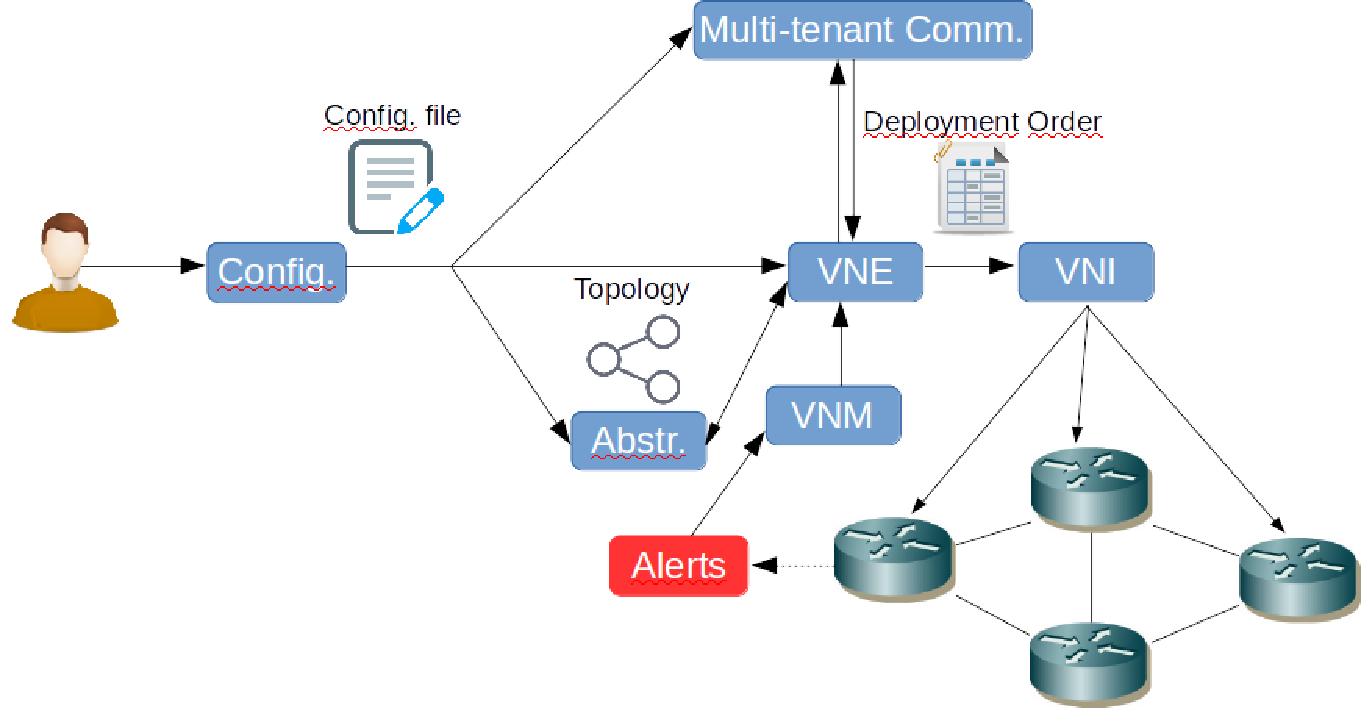
\includegraphics[scale=0.7]{figures/network-hypervisor-workflow}
% \caption{Deploying a topology in a network hypervisor.\label{fig:Workflow}}
% \end{figure}

% \subparagraph{\textbf{Migration}}\textbf{}\\
% The migration component collects alerts from the infrastructure about failures or resource congestion.
% Figure~\ref{fig:Workflow} illustrates how the component receives an infrastructure alert and transmits it to the VNE component so he can recompute the topologies.

% During runtime, a user may push a request for resources.
% This request is transmitted to the RAC for verification.
% If the request can be granted, the RAC will notify the VNI to deploy the resources.
% Oherwise, an error should be raised and returned to the user.





\subsubsection{Summary}
We have presented a reference based on existing network hypervisors using the SDN paradigm.
Table~\ref{tab:comparison-refarchi} summarizes it and shows how each hypervisor implements the different modules of the reference architecture.
Both DPAC and CPAC are implemented in every hypervisor, as they are essential for a basic support of network virtualization.
The control over the VN exposed by the CPAC is either hypervisor based (HB) or full control (FC).
% Openflow~\cite{Openflow-McKeown2008} is the main implementation for the DPAC as it is a standard supported by the industry and is widely studied.
Maintaining a mapping between physical and virtual resources in the DPAC has become a main goal since arbitrary topologies often come with flowspace virtualization, thus giving tenants a lot of flexibility.
Only Compositional Hypervisor~\cite{CompositionalHypervisor-Jin2014} does not properly virtualize the dataplane and interact with it using OpenFlow~\cite{Openflow-McKeown2008}.
In a similar way, the VNE algorithms greatly simplifies the administration of virtual networks and thus has been integrated since early prototypes.
While FlowVisor provides CPU and bandwidth (BW) isolation, only Slices Isolator~\cite{SlicesIsolator-El-Azzab2011} and Double FlowVisor~\cite{DoubleFV-Yin2013} extend this isolation to the interfaces (Int) of a switch as well as the memory (Mem).
We observe that few solutions have implemented an advanced monitoring module (\ie monitoring more than Discovery Protocols Notifications).
In addition to that, network hypervisors rarely address the migration problem, leaving a lot of work to do to researchers.




% Please add the following required packages to your document preamble:
% \usepackage{multirow}
% \usepackage{graphicx}
\begin{table}[]
\centering
\resizebox{\textwidth}{!}{%
\begin{tabular}{|c|c|c|c|c|c|l|}
\hline
Name                                                            & CPAC                      & DPAC          & Topology      & VNE & VNM & Security \\ \hline
FlowVisor~\cite{FlowVisor-Sherwood2009}                         & \multirow{6}{*}{FC} & Proxyfication & Not arbitrary & No  & No  & No       \\ \cline{1-1} \cline{3-7} 
ADVisor~\cite{ADVisor-Salvadori2012}                            &                           & Mapping       & Arbitrary     & No  & No  & No       \\ \cline{1-1} \cline{3-7} 
VeRTIGO~\cite{VeRTIGO-Corin2012a}                               &                           & Mapping       & Arbitrary     & Yes & Yes & No       \\ \cline{1-1} \cline{3-7} 
Enhanced FlowVisor~\cite{EnhancedFV-Min2012}                    &                           & Proxyfication & Not Arbitrary & No  & No  & No       \\ \cline{1-1} \cline{3-7} 
Slices Isolator~\cite{SlicesIsolator-El-Azzab2011}              &                           & Proxyfication & Not Arbitrary & No  & No  & No       \\ \cline{1-1} \cline{3-7} 
Double FV~\cite{DoubleFV-Yin2013}                               &                           & Mapping       & Arbitrary     & Yes & No  & No       \\ \hline
Compositional Hypervisor~\cite{CompositionalHypervisor-Jin2014} & FC                  & Openflow      & Not Arbitrary & Yes & No  & No       \\ \hline
CoVisor~\cite{CoVisor-Jin2015}                                  & FC                  & Mapping       & Arbitrary     & Yes & Yes & Yes      \\ \hline
FlowN~\cite{FlowN-Drutskoy2012}                                 & HB                       & Mapping       & Arbitrary     & Yes & Yes & No       \\ \hline
Network Hypervisor~\cite{NetworkHypervisor-Huang2013}           & HB                       & Mapping           & Arbitrary     & Yes & No  & No       \\ \hline
AutoSlice~\cite{AutoSlice-Bozakov2012,AutoSlice2-Bozakov2014}   & FC                  & Mapping       & Arbitrary     & Yes & Yes & No       \\ \hline
NVP~\cite{NVP-Koponen2014}                                      & FC                  & Mapping       & Full Mesh     & No  & Yes & Yes      \\ \hline
OpenVirteX~\cite{OpenVirteX-Al-Shabibi2014}                     & FC                  & Mapping       & Arbitrary     & Yes & No  & No       \\ \hline
SR-PVX~\cite{PVX-Li2017}                                        & FC                       & Mapping       & Arbitrary     & Yes & No  & No       \\ \hline
WhiteVisor~\cite{whitevisor-Yu2019}                             & FC                 & Mapping       & Arbitrary     & Yes & No  & No       \\ \hline
ONVisor~\cite{ONVisor-Han2018}                                  & HB                       & Mapping       & Arbitrary     & Yes & No  & Yes      \\ \hline
LiteVisor~\cite{Litevisor-Yang2018}                             & FC                  & Mapping       & Arbitrary     & Yes & Yes & No       \\ \hline
\end{tabular}%
}
\caption{Comparison of the network hypervisors with the reference architecture}
\label{tab:comparison-refarchi}
\end{table}

\newpage
\section{Migration of virtual networks with SDN}
\label{sec:sota-vnmigration}
In this section, we discuss the different virtual network migration solutions.


\subsection{Preliminary work}

We start by presenting solutions published on the same year as OpenFlow and that have been used as a reference in a majority of SDN-based migration solutions.

\subsubsection{VROOM}
Virtual ROuters On the Move (VROOM)~\cite{VROOM-Wang2008} is an early work discussing how the migration of virtual routers should be implemented on top of the physical infrastructure. 
VROOM outlines that most of the network state changes are caused by planned maintenance.
Moreover, power consumption is also a primary concern because efficient migrations can save up to hundreds of millions of dollars.
In this regard, VROOM presents a network virtualization and migration technique aiming at minimizing these costs and the duration of maintenance.
VROOM is composed of 3 building blocks: router virtualization, data and control plane separation, and dynamic interface binding.
Router virtualization is already implemented in some commercial routers, and VROOM presents two prototypes, one software based and the other one hardware based.
Data and control plane separation is achieved by using different virtualization environments (VE) in a virtualization infrastructure, namely OpenVZ~\cite{openvz}.
The data plane is implemented using OpenVZ first VE (VE0) in which the software implementation of the VROOM router will use a Linux kernel in a commodity server while the hardware implementation will use a NetFPGA circuit.
The control plane is also implemented using OpenVZ but using separate VEs (VE1, VE2, ...).
Each virtual router is stored in a VE, in which a kernel and routing protocol are implemented using a software suite.
The binding of physical interfaces with virtual interfaces is divided into two mappings.
The first one implements the mapping of the virtual router with the corresponding Forwarding Information Base (FIB) inside the physical router.
The second one is the mapping of the FIB of the physical router with a corresponding physical interface.

\subsubsection{Virtual Network Embedding and path migration}
Yu~\etal proposed in~\cite{VNE-Yu2008} a VNE model designed to support the splitting of a virtual link over several physical links, as well as dynamic virtual network reconfiguration.
The whole work is intended to improve resource allocation and maximize the acceptance rate. 
Path splitting takes a virtual link with a required amount of bandwidth that cannot be embedded on the physical infrastructure, and divides it into several smaller links that can be accepted by the infrastructure.
Several VNE algorithms are proposed, including one tailored to fit a type of topology that is expected to be common.
Path migration extends the usability of path splitting by allowing to recalculate the embedding of existing virtual networks and freeing extra resources otherwise not available using path splitting solely.
The authors provide an extensive evaluation of their mapping and migration algorithms using a simulator~\cite{vnesimulator}.

Both~\cite{VROOM-Wang2008} and~\cite{VNE-Yu2008} have been published on the same year as the publication of OpenFlow~\cite{Openflow-McKeown2008}, an implementation of the Software Defined Network paradigm that will become the standard of SDN for both industry and academia.
Despite the fact that these publications are not based on SDN, they set up guidelines for plenty of the works we will now describe.

We divide the existing VN migration solutions based on the research issue they tackle.
% \GB{the categorization seems to explore 3 different objectives, and it is difficult to see the logic of such categorization}
We summarize these issues into three categories: 
\begin{inparaenum}[i)] 
\item the migration is designed to improve the global performance of the infrastructure;
\item the migration was implemented to explore existing technical limitations with regard to virtualization platform; or 
\item the solution explores the migration from a formal perspective.
\end{inparaenum}

\subsection{Improving the performance of the infrastructure}
% Ye~\etal propose in~\cite{Ye2017a} a resource utilization model in which they aim to maximize the resource allocation on switches while looking to determine controllers that can be shut down due to underutilization and migrate switches.
% Authors solve the resource allocation problem using optimization under constraints techniques. 
% The switch migration problem is described as NP-hard and is approximated using a Log-sum-exp approximation.
% This approximation determines the allocation of network switches on controllers that will maximize their utilization. 
% From this distribution, authors construct a Markov chain that represent the different distributions strategies and where transitioning from a state to another corresponds to migrating a switch from a controller to another controller.

% In~\cite{Wang2017d}, Wang \etal study a problem similar to~\cite{Ye2017a}, but are more focused on the migration and its efficiency, and present a Switch Migration-based Decision Making (SMDM) scheme. The problem is divided into three parts: detecting the overload of the controller due to an excessive amount of OF requests, the modeling of the migration's performance and finally, modeling the trade-off between the profit generated by the migration and the cost it incurred.
% The overload detection correlates two types of information to determine overloaded controllers.
% The first one is the actual amount of requests received by controllers, while the second is the load ratio between each pair of controllers.
% This ratio is then bound to a threshold above which a migration will be triggered to relieve one controller from its load and reallocate it to the other.
% Modeling the efficiency of the migration considers both the load variation of the controllers as well as the overhead of messages exchanged to implement the migration.  
% Finally, the migration strategy is in charge of determining which switch should be selected as the next candidate for the migration and where it should be migrated.
% Figure~\ref{fig:smdm-wang2017d} illustrate the interactions of the different components of the solution.

% \begin{figure}[ht]
%     \centering
%     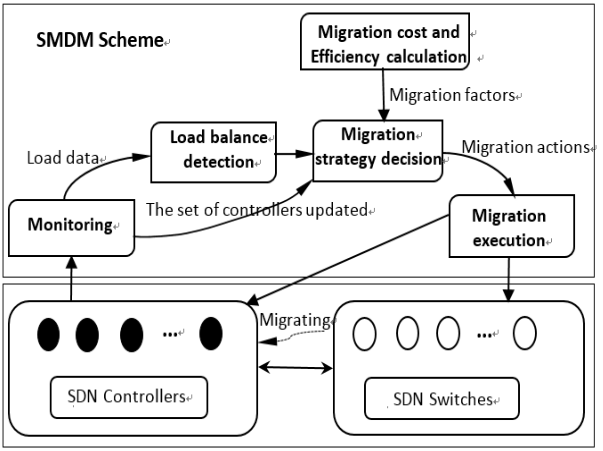
\includegraphics[scale=0.65]{figures/wang2017d.png}
%     \caption{Architecture of the SMDM scheme~\cite{Wang2017d}}
%     \label{fig:smdm-wang2017d}
% \end{figure}

Lo~\etal introduce in~\cite{vnm-lo2013} the design of a virtual network migration process.
The cost of the migration is based on two metrics, the completion time of the migration as well as the bandwidth consumption.
Based on the original embedding and the new destination substrate, the goal is to determine the ordering of node migration that will minimize the cost of the migration.
For each step in the migration, the time taken to migrate a node is divided into two parts. The first one represents the time taken to prepare the migration and the second one is the time taken to actually transmit information to the destination substrate.
The cost of a migration step is the product of the time it takes to migrate the information with the impact the migration incurs on the bandwidth.
Virtual nodes are categorized based on whether the node:
\begin{inparaenum}[i)] 
\item has been migrated;
\item will be at this step of the migration; or 
\item will be migrater at a later step.
\end{inparaenum}
Similarly, the virtual links' are divided into three categories based on whether the nodes composing the links:
\begin{inparaenum}
\item have been migrated;
\item will be migrated; or 
\item will not be migrated.
\end{inparaenum}
The categorization of virtual resources is then used to determine the cost of the migration.
Three different virtual network migration algorithms are presented, differentiated by the fact that nodes may be either migrated one node at a time or multiple nodes may be migrated together.
% \GB{three algorithms but only 2 are mentioned. and don't you ever use ``whether'' again?}
The first algorithm is a greedy iteration over the individual costs of migrating each node.
The second algorithm is designed to minimize the migration time. Since migrated nodes are constrained to be independent from other nodes, the algorithm determines the biggest set of independent nodes.
Then, the algorithm leverages the fact that several nodes can be migrated simultaneously to reduce the total migration time.
The third algorithm is a combination of the first two, where a tradeoff between migration time and migration cost is sought. The algorithm computes the different sets of independent nodes, and instead of choosing the largest one, choose the set with the smallest cost.
Again, this algorithm uses the simultaneous node migration to choose the set with the smallest cost.

Robust virtual network migration is studied in~\cite{Ko2017c}. The authors outline that traditional migration suffers from down times proportional to the size of the migrated virtual networks, while protection mechanisms cannot be adapted to support the dynamic changes in the network.
Three requirements are defined while considering drawbacks of existing migration techniques. 
First, the tenant's controller should never be notified of the migration.
Second, the migration process should account for the network traffic status inside the physical infrastructure.
Finally, the migration process should minimize the number of interactions between the network hypervisor and the physical infrastructure.
Protection and restoration techniques are described to account for these requirements.
Protection consists in deploying backup paths on the physical nodes, calculated prior to any incident.
This way, in case of a failure, the traffic can immediately be routed through the alternative path. 
This method implies that the hypervisor must maintain regularly updated backup paths in each node, incurring computational overhead, bandwidth consumption on the physical resources of the switch.
Restoration is the case where all the backup paths are stored inside the network hypervisor and only deployed in case of a failure.
This method is based on the assumption that failures will rarely happen, thus it will not generate an important number of messages between the infrastructure and the hypervisor.
The network hypervisor determines a backup path that will minimize the amount of messages sent to the infrastructure.
To do so, the backup path must use the same links as the original while only differing at the failure point.
Updates of backup paths are performed regularly while a monitoring device collects statistic on available resources to determine if the current backup paths can still be used.
The migration solution is implemented using OpenVirteX~\cite{OpenVirteX-Al-Shabibi2014}, where the path calculator and storage mechanisms are adapted to fit the new requirements. 
% Then new components related to the prioritization of backup paths, updating existing paths and monitoring the physical network are implemented and integrated into the hypervisor.

Improving the revenue generated with network virtualization can be done through migration.
In~\cite{fragment-Liu2018}, the purpose of VN migration is to optimize the acceptance ratio of new virtual network requests as well as the revenue to cost ratio.
While traditional VNE algorithms only rely on the individual capacities of nodes, they do not consider the possibility to split the bandwidth over multiple links.
To this end, the notion of fragment degree for a virtual node is introduced and is defined as a weighted combination of the CPU consumption ratio of the virtual node on its embedding node and the bandwidth consumption ratio of adjacent virtual links on the physical substrate.
The fragment degree of each virtual node is then associated with the embedding cost of existing virtual networks into a multi-objective integer linear program. The solution of this program being NP-hard to solve, the authors propose a novel algorithm to make it computationally tractable: Fragment-aware Virtual network Reconfiguration (FA-VNR).
This algorithm first defines a migration trigger. 
% Maximizing revenue over time pushed for a periodical migration of VNs.
Then, it determines which set of physical nodes must be reconfigured by computing a dynamic threshold of ``fragmentation" in the infrastructure.
Similarly, the algorithm determines a set of virtual nodes to migrate based on their economical performance.
Once the destination substrate has been chosen, virtual nodes will be migrated and each virtual link connected to them will be redeployed using a shortest path algorithm.

\subsection{Evaluating virtualization platforms}
We present here two migration solutions that have been implemented on a particular physical infrastructure.
Both solutions aim at outlining the technical limitations faced when migrating VNs.

\subsubsection{PlanetLab}
PlanetLab~\cite{Chun2003d} (PL) is a virtualization infrastructure used to provide slices of network resources for research experiments. Lo~\etal state in~\cite{Lo2014} that VN migration is a field where practical implementation and evaluation remain to be explored. They proposed a migration scheme and implemented it in PL, namely PL-VNM. The migration should be designed to be automated, fast and to minimize the service disruption time. While the migration process is automated, there is no detection component to automatically trigger the migration. Due to technical limitations of PL, it is impossible to migrate a VN from a slice to another. An alternative is proposed by partitioning the resources within a slice thus defining new virtual networks inside a PL slice and limiting the migration to the VNs created in a single slice. Virtual routers are instantiated for each virtual node required by the topology, and use an API to install forwarding rules in the kernel space of the physical node.
The authors proprose a simple migration algorithm based on the size of the flows to migrate.
The migration process consists in cloning the network state of virtual nodes (\ie FIB) and then  redirect VMs' traffic through the newly created virtual network.
While the duplication of networking state does not cause any packet loss from the tenant's point of view, setting up the redirection is most likely to create service disruption.
Two different approaches are taken and evaluated.\\
The first approach consists in preparing the scheduling for the host redirection and then sequentially send commands to the gateways connected to the hosts, namely remote scheduling.
Figure~\ref{fig:plvnm} depicts the modules of PL-VNM and how the migration process is handled.
One of the drawbacks of this method is the delay existing between the migration instruction being sent by the controller and the instruction actually being run at the gateway.\\
The second approach relies on determining the migration ordering and then scheduling the migration in the gateway using the UNIX command \textit{at}. The \textit{at} command makes sure that the migration is performed on time by synchronizing the gateway via the NTP protocol. Here, the potential latency to execute the migration is based on the time it takes for NTP to trigger \textit{at} and on the load of the gateways' CPU.
Both approaches make it hard to have a full control over the migration's timing.
The authors conclude with three recommendations for the PL infrastructure and in general for network hypervisors.
\begin{inparaenum}[i)]
\item Enabling gateway task scheduling with a magnitude order of milliseconds. As is, \textit{at} scheduling uses seconds for tasks triggers while path latency of remote scheduling is a few hundreds of ms;
\item Allowing the migration scheduler to order migration commands to reduce the delay induced in the actual start of the command;
% \GB{to be rewritten}
\item Implementing asymmetric packet routing inside the infrastructure.
Because of the routing mode used in PL, each link in the gateway must have the same physical source and destination, thus preventing an asymmetric migration of the FIB from being effective. 
\end{inparaenum}

While~\cite{Lo2014} is not specifically designed to work on an SDN infrastructure, the problems and challenges it explores remain valid in the SDN paradigm.

\begin{figure}[ht]
    \centering
    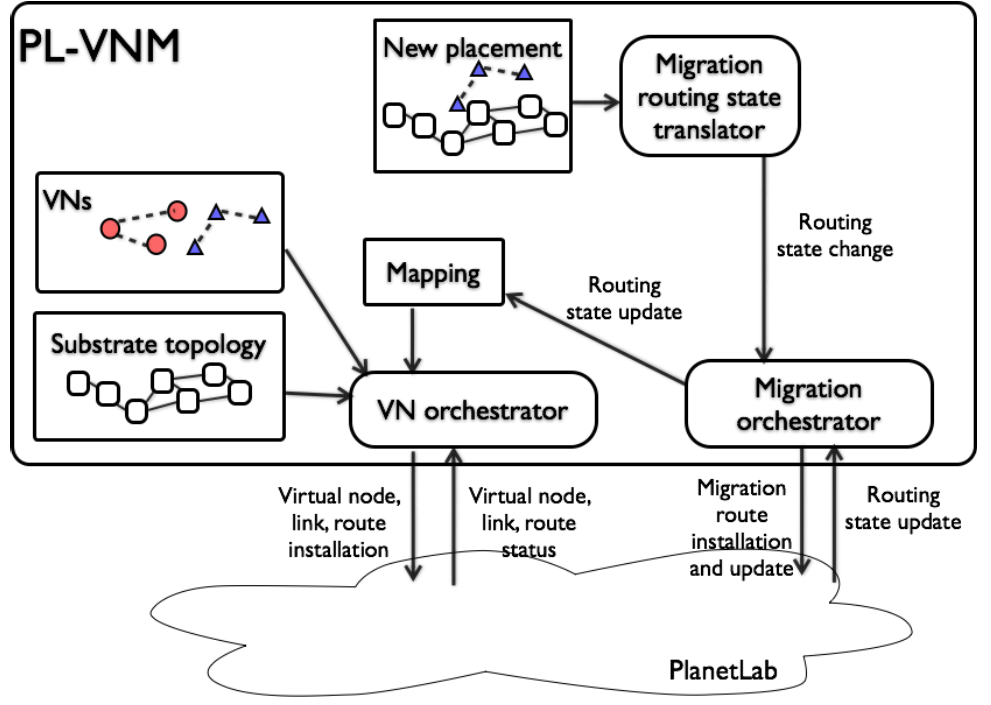
\includegraphics[scale=0.5]{figures/pl-vnm.png}
    \caption{Architecture of PL-VNM~\cite{Lo2014}}
    \label{fig:plvnm}
\end{figure}

\subsubsection{GENI}
The GENI platform~\cite{GENI-Berman2014} is a network infrastructure based on SDN and used to provide isolated environments for researchers to run experiments.
Zhao~\etal propose in~\cite{Zhao2017} a VN migration scheme implemented using GENI. 
Similarly to PlanetLab, GENI has not been designed to support the migration of VNs over different physical substrates. 
We differentiate \textbf{slice} from \textbf{Virtual Networks (VN)} in~\cite{Zhao2017}.
A \textbf{slice} is a GENI slice, \ie the set of resources allocated to a tenant, while \textbf{VN}  are a subset of these resources.
Implementing VNs (original and migration backups) can be done by allocating all required resources to a single slice. This approach comes with drawbacks however: no clear isolation between VNs, lack of flexibility in case there is a need for a topology change. Finally, in case of a failure of a VN or a host, the whole topology must be rebuilt.
Another approach consists in allocating one slice for a single VN and then, when migrating it, allocating a new slice. The main challenge is to set up communication between the old and the new slice during the migration, since GENI enforces isolation between its slices.
In addition to the inter-slice communication, the migration process should not cause packet loss and be invisible to the tenant.
A proposed approach separates the old VN, the new VN and the VMs by setting up a different slice for each group. Two extra gateways are inserted in the VMs' slice, each connected to one of the other slices.
Without these gateways, the learning switch implemented by GENI would not allow to connect the hosts to the new VN because of conflicting rules (same source/destination, different output ports).
The three slices will then share a common VLAN to communicate together.
In order to minimize the packet loss incurred by the migration, the migration is optimized by scheduling the sequence of flows that will be deployed on the physical substrate.
First the rules between gateways and the new VN are set up, then the hosts' traffic is redirected towards the second gateway and finally old VN rules are dropped leading to a full disconnection of the former VN.
A similar problem to the migration in PlanetLab concerns the migration scheduling on the physical switches.
The first option is to remotely control network interfaces using SSH.
An SSH connection with each switch is established and old interfaces will be shut down while activating the new ones.
However, the latency induced by SSH authentication and by the time it takes to transmit commands makes the migration unpredictable.
On the other hand, the migration can be performed by sending OF rules as the migration progresses. This method is deemed faster than the other one since it does not use SSH (and its authentication overhead), but it is thus less secure.
Finally, the transparency of the migration is ensured by the migration controller who will act as a proxy between VNs and switches, intercepting packets and rewriting header fields to maintain a consistent view of the network.

\subsection{Formal verification of the migration}
In complement to the works aiming at improving the performance and the scalability of the virtualization infrastructure and the migration process, we now consider the works taking a formal approach to study specific properties of the migration and the migration process. 
% \GB{ok but to what ends?}
The following approaches contrast with the previous ones because they characterize specific properties of the migration of virtual networks instead of focusing on operational aspects. 

\subsubsection{Inter-flow consistency}
In an SDN infrastructure, the configuration deployed on SDN switches gets updated and evolves regularly. Such modifications are invoked by the SDN controller and deployed among several switches.
Flow consistency ensures that each flow will be processed by either the old or the new configuration all along the way, and not by a combination of the two.
However, Liu~\etal argue in~\cite{Liu2015a} that making sure that each individual flow has its own consistency preserved is not enough to respect certain security and reliability requirements.
It becomes necessary to model relationships between flows and to preserve certain properties throughout the migration.
The properties considered here are spatial isolation and version isolation.
The spatial isolation of two flows consists in preventing them from sharing a common physical resource before, during and after a change in the network configuration.
For instance, a critical flow carrying important information should not share a link with a certain traffic that may be subject to surges, thus leading to link congestion and the important flow not being delivered. Another case would be when attackers would try to intercept information on critical flows and then exploit the infrastructure.
Version isolation ensures that a configuration affecting different flows is fully deployed and prevents one flow being processed with one configuration and another flow with another version of the configuration.
This problem is related to the delay in actually deploying the configuration inside the switches, as outlined with PlanetLab and GENI.
The spatial isolation problem is approached using a dependency graph. Each path taken by a flow is mapped with the physical nodes they go through. Then, in case of overlapping node for several flows, the node is seen as a mutex node (similarly to the mutex of an operating system).
No flow may go through a mutex node if another flow is currently using it.
This ensures that specific traffic may not cohabit inside the same physical resources.
To ensure the version isolation of different flows, the system identifies the set of flows that must be isolated. Then, it picks one to be processed normally and forward to the controller all the traffic of the remaining flows. This way, it makes sure that there are not two flows being processed by 2 different versions of a configuration. And when all the cached traffic is re-injected inside the infrastructure, it is being processed by a fully updated networking state.

The generation of the dependency graphs is done by categorizing flows into two classes, based on whether they should be forwarded to the hypervisor or not. Using a greedy algorithm, we can determine how to minimize the amount of packet caching that would be done at the controller.
The ordering of the migration sequences is determined from the graph. Each sequence is composed of several configuration modifications, and these modifications are also ordered to minimize the migration time. 

\subsubsection{Moving Target Defense}
Dynamically changing the location of sensitive targets is a technique called Moving Target Defense (MTD). Such changes prevent an attacker from accurately knowing the attack surface of the system he is attacking. 
% because the configuration regularly changes. 
% \GB{all the segment on the works of Chowdhary does not really concern migration. you may drop it}
Chowdhary~\etal~\cite{Chowdhary2016} use MTD techniques as part of a Detect-Analyze-Counter cycle inside an SDN-based Cloud infrastructure. 
The security system is composed of four modules: a detection module, a vulnerability analyzer, a counter-measure creation and deployment component and a policy conflict resolution.
The detection module is in charge of gathering information about the vulnerabilities in the infrastructure.
Then, the analyzer will use these information to dynamically generate an attack graph representing the capacities of the attacker. 
A counter-measure will then be generated to mitigate the potential attacks and be proposed to the conflict resolution module. This module  will determine if the newly created counter-measure is not going to have any harmful side effects. Once the counter-measure is accepted it is deployed in the infrastructure and the detection module is notified of the new configuration. 
The attack detection aspect is left out in this paper, as it is already a widely explored topic.
A well known drawback of attack graphs is the poor scalability when the number of states grows.
This problem makes the graph generation computationally intractable. Partitioning the attack graph into smaller regions based on each tenant using the infrastructure simplifies the generation.
These sub-attack graphs are then simply merged together for the counter-measure to be generated.
The counter-measure component determines which VM should be migrated based on the CVSS Base Score.
Once the target VM is chosen, new flow rules are computed to implement the migration. 
The conflict resolution inspects the flow rules that should be deployed and extracts the actions of each rule and verify that they do not overlap with other existing flow rules. If a conflict arises, this module will try to find alternative rules. In the event where this would not be possible, the proposed counter-measure is rejected and a new one is computed.

\subsubsection{Seamless migration}
In the previous works, minimizing the service disruption caused by the migration has always been a major concern in the design of the solution. However, while the efficiency of the solution was evaluated with various experiments, there was no formal approach describing the transparency of the migration and ensuring that no disruption of service will be experienced by a tenant.
The topic of seamless migration is brought up in~\cite{toward-Ghorbani2014} where Ghorbani~\etal take a closer look at network virtualization using SDN techniques.
Precisely, the focus is put on the one-to-many mapping, also known as the ``Big Switch" abstraction.
Distributing a single virtual resource over several physical ones may not preserve the per-flow correctness.
Similarly to the version isolation presented in~\cite{Liu2015a}, flow correctness considers flows individually and ensures that each packet of each flow  is always processed by one specific version of a network configuration. 
% Version isolation ensures that flows are processed by a single global configuration while flow correctness ensures that end points receive packets in the proper order to avoid errors at the application level.
However, this definition does not ensure that the ordering of packets as seen by the tenant's applications and controllers is a good representation of how the packets were originally sent and ordered by the other end point.
A new definition of correctness is proposed to make sure that the ordering of packets is preserved from end to end.
From this definition  a solution for a seamless migration of VNs and VMs is proposed in LIME~\cite{Lime-Ghorbani2014}.
The first contribution of this paper is a formal model for network virtualization migration, and it defines a transparency property related to the physical observation of the migration.
The second is an implementation of a virtual network migration process that is proven to respect the transparency property previously defined.
It is important to note that transparency does not exclude packet loss but is aimed to reduce it drastically.
The migration of the virtual network resources relies on switch cloning.
LIME will instantiate several copies of each virtual node and orchestrate the migration so the tenant's traffic is still forwarded during the migration.
In opposition to the requirement made in~\cite{Ko2017c}, LIME will notify the tenant application in case of a physical failure of a link.
Ghorbani~\etal then use the formal model to extend the transparency property to the one-to-many mapping problem of~\cite{toward-Ghorbani2014}.
Since the idea is to propose a ``Big Switch" abstraction while  the virtual resource is being replicated across several physical nodes. The point is to make sure that all nodes located on the edge of the Big Switch are preserving the ordering of the packets even when the configuration is updated.
The observation correctness introduced in LIME is enhanced with the concept of weak causality where an event has weak causal dependency with another if the first event has triggered the other under certain conditions.
Thus, the observable ordering of events will matter only if those events are correlated.


\subsection{Summary}
The study of VN migration remains a topic of interest as it has been studied but often with the same objective: creating a migration process that will improve the performance of the infrastructure. 
Table~\ref{tab:existing-vnm} summarizes the surveyed works. Several types of algorithms are proposed, usually either a migration scheduling algorithm or a VNE-related algorithm. 
The bandwidth remain the most common metric used, as it is one of the main criteria to support virtual networks. Other operational metrics like migration duration or CPU consumption are used for performance improvement.
The migration process has not been studied under the security perspective.
This should be investigated to propose a model of the security of the migration process, its properties and how can they be observed and verified. From an architectural point of view, users are not presented with their own virtual network that they will be able to configure, but instead the manipulation of the physical infrastructure is abstracted to implement an efficient OF rules deployment and to allow the coexistence of heterogeneous solutions.

% Please add the following required packages to your document preamble:
% \usepackage{graphicx}
% \GB{please insert authors' names in the reference column of Table~\ref{tab:existing-vnm}}
\begin{table}[h]
\centering
\resizebox{\textwidth}{!}{%
\begin{tabular}{|l|l|l|l|}
\hline
\textbf{Reference}       & \textbf{Algorithms}                                                                                                          & \textbf{Metrics}                                                                              & \textbf{Summary}                                         \\ \hline
Wang~-~\cite{VROOM-Wang2008}    & N/A                                                                                                                          & \begin{tabular}[c]{@{}l@{}}Power consumption\\ Bandwidth\\ CPU\end{tabular}                   & Early prototyping virtual network migration              \\ \hline
Yu~-~\cite{VNE-Yu2008}        & \begin{tabular}[c]{@{}l@{}}Link/Node mapping\\ Path splitting\\ Path migration\\ Custom topology mapping\end{tabular}        & \begin{tabular}[c]{@{}l@{}}CPU\\ Bandwidth\\ Request processing time\end{tabular}             & Migration to improve the acceptance ratio                \\ \hline
Lo~-~\cite{vnm-lo2013}        & \begin{tabular}[c]{@{}l@{}}Greedy minimum cost\\ Biggest set of independent nodes\\ Biggest set  + minimum cost\end{tabular} & \begin{tabular}[c]{@{}l@{}}Migration duration\\ Bandwidth\end{tabular}                        & Scheduling algorithms for the migration                  \\ \hline
Ko~-~\cite{Ko2017c}           & Backup path computation                                                                                                      & Bandwidth                                                                                     & Migration module on top of OpenVirteX                    \\ \hline
Liu~-~\cite{fragment-Liu2018}      & \begin{tabular}[c]{@{}l@{}}Target selection\\ VNE\end{tabular}                                                               & \begin{tabular}[c]{@{}l@{}}CPU\\ Bandwidth\end{tabular}                                       & Improving the acceptance ratio                           \\ \hline
Lo~-~\cite{Lo2014}            & Flow size based migration                                                                                                    & \begin{tabular}[c]{@{}l@{}}Packet loss\\ Migration time\end{tabular}                          & Implementing VN migration on PlanetLab~\cite{planetlab}  \\ \hline
Zhao~-~\cite{Zhao2017}          & Seamless traffic redirection                                                                                                 & \begin{tabular}[c]{@{}l@{}}Packet loss\\ Migration time\\ Control plane overhead\end{tabular} & Implementing VN migration on GENI~\cite{GENI-Berman2014} \\ \hline
Liu~-~\cite{Liu2015a}          & \begin{tabular}[c]{@{}l@{}}Flow classification\\ Mutex nodes\\ Migration scheduling\end{tabular}                             & \begin{tabular}[c]{@{}l@{}}Bandwidth\\ Memory\end{tabular}                                    & Consistent flow processing during configuration changes  \\ \hline
Chowdhary~-~\cite{Chowdhary2016}     & \begin{tabular}[c]{@{}l@{}}Attack graph analysis\\ Counter measure selection\end{tabular}                                    & Vulnerabilities                                                                               & VN migration for VM security                             \\ \hline
Ghorbani~-~\cite{Lime-Ghorbani2014} & \begin{tabular}[c]{@{}l@{}}Node cloning\\ Iterative migration\\ Simulataneous migration\end{tabular}                         & \begin{tabular}[c]{@{}l@{}}Latency\\ Packe loss\\ Bandwidth\\ Network updates\end{tabular}    & Formal verification of the seamless migration            \\ \hline
\end{tabular}%
}
\caption{Summary of VN migration}
\label{tab:existing-vnm}
\end{table}


\subsection{Network \& VM security}

We have presented in the previous sections the existing solutions for network virtualization and virtual network migration. We now delve into the security aspect of network virtualization, and the related topics. The security of virtual migration is a topic that has never been properly studied yet, while the security of VM migration has been thoroughly investigated. Following sections cover two main topics, namely the security of the VM migration process and existing formal models for network security.

\subsubsection{Security of VM migration}

In this section we take a closer look at the security of the live migration of VMs.
We first detail the existing vulnerabilities and attacks possible and then detail different security solutions, either using the migration process as a way to overcome security issues or that analyze and improve the security of the migration process itself.

\paragraph{Attacking the VM migration process}
Traditional hypervisors have been around for decades now, and the live migration of a virtual machine is a well known process. There has been several security surveys on the topic of VM hypervisors~\cite{Reuben2007,Rehman2013,Sahoo2010,Perez-Botero2013}, and on the security of Cloud environments~\cite{cloudenvironmentsecuritysurvey-fernandes2014}.
Most of the security issues with VMs are related to the unlawful interactions between a VM and other VMs or the hypervisor.
An attacker may exploit vulnerabilities in the hypervisor and force it to execute arbitrary code or access restricted memory zone.
Another type of attack consists in corrupting the resource scheduler of the hypervisor, thus preventing other users to get the allocated resources they deserve.

We will focus here on the attacks that can impact the live migration of a VM.
Oberheide~\etal proposed in~\cite{empirical-oberheide2008} several attack classes that will affect the migration of VMs: attacks on the control plane, the data plane and the migration module.
These attacks are summarized in Table~\ref{tab:vm-attacksurface}.

Attacks impacting the control plane can be divided into two categories: resource exhaustion and hypervisor spoofing. The attacker is triggering an unlawful migration to either move a VM toward an unsecured physical location or to overload the local hypervisor and preventing a legitimate user to be served with his due resources.

The second attack class is Fake Resource Advertising. This kind of attacks are particularly efficient in systems where the migration is automated, because the generation of fake servers inside the topology can make the hypervisor trigger migration of VM on resources that do not exist.
Attacking the data plane during the live migration can take two forms: passively exfiltrating sensitive information or actively altering the traffic during the migration.
In the first case, the attack results in a loss of confidentiality for the stolen data and it might be exploited later on to launch other attacks on the VM.
In the second case, altering the traffic can either create a Denial-of-Service because the VM virtual disk has been compromised, or in a potentially even more harmful scenario the VM keeps working but under a compromised state, as the ongoing processes may not function with expected data.

The VM migration module can also be attacked to allow an attacker to have his VM share the same physical server with his victim's VM. Stalling the migration is studied in~\cite{stalling-atya2017} where the attacker prevents his and his victim's VMs from being separated so he can completely invalidate the memory pages of the victim's VM. It is shown that maintaining the co-residency between the VMs allows an attacker to use side channels attacks that will have a bigger impact on the victim.
% A presentation on these side channel attacks is detailed in~\cite{malicious-atya2017}.

% Please add the following required packages to your document preamble:
% \usepackage{multirow}
% \usepackage{graphicx}
\begin{table}[ht]
\resizebox{\textwidth}{!}{%
\begin{tabular}{|c|c|c|}
\hline
Attack                     & Methodology                                                                             & Impact                                       \\ \hline
\multicolumn{3}{|c|}{Control Plane}                                                                                                                                 \\ \hline
Incoming migration         & \multirow{2}{*}{Resource exhaustion}                                                    & Co-residency of the victim with the attacker \\ \cline{1-1} \cline{3-3} 
Outcoming migration        &                                                                                         & Overload of the hypervisor                   \\ \hline
False resource advertising & Hypervisor spoofing                                                                     & Unifying heterogeneous SDN applications      \\ \hline
\multicolumn{3}{|c|}{Data Plane}                                                                                                                                    \\ \hline
Passive Snooping           & Network probe                                                                           & Information leakage                          \\ \hline
Active manipulation        & Network man-in-the-middle                                                               & Data corruption                              \\ \hline
Host identification        & \begin{tabular}[c]{@{}c@{}}Network monitoring\\ Migration characterization\end{tabular} & Specific targeting for future attackst       \\ \hline
\multicolumn{3}{|c|}{Migration module}                                                                                                                              \\ \hline
Software attacks           & Heap, stack, integer overflow                                                           & Service disruption, Incorrect behaviour      \\ \hline
\end{tabular}%
}
\caption{Attack surface of live VM migration}
\label{tab:vm-attacksurface}
\end{table}

\paragraph{Protecting the VM migration process}
The Moving Target Defense (MTD) paradigm is a technique used to limit the co-residency between an attacker and its victim, thus leading to a reduced attack surface for side channel attacks.
Zhang~\etal introduce a Game Theory model~\cite{incentivemtd-Zhang2012} to represent the incentives a Cloud Provider has to migrate VMs in his infrastructure when opposed to an attacker who will benefit from the co-residency. Results outline that it is not necessary to permanently migrate all VMs and only a subset of them. In addition to this, the game can be extended to include cooperation between the legitimate users and the Cloud Provider.
A similar approach using MTD against side channel attacks is presented in Nomad~\cite{nomad-Moon2015b}. Nomad is built on the assumptions that the attacker cannot be precisely located inside the infrastructure, can launch potentially unknown side channels attacks and can precisely target his victim. 
The migration process proposed in Nomad provides tenants with an API to describe a set of constraints on their VM that has to be respected throughout the migration.
Nomad provides a scalable VM placement algorithm, a framework that does not require to modify the OS, the hardware or the hypervisor, other than the migration algorithms.
The protection of the migration traffic by making it indistinguishable from regular network traffic using noise generation is studied in~\cite{stealth-Achleitner2017a}. Even if encryption is applied to the migration traffic, an attacker located inside the infrastructure may still distinguish migration traffic from the regular one. Indeed, migration traffic can easily be characterized as a set of data bursts through the network. The proposed solution uses a token bucket traffic generator to implement a white noise that will dynamically adapt to the traffic generated by the migration. This method will make the migration traffic look like a constant flow of indistinguishable data.



\subsubsection{Formal Models for network security}

Formal models for network security cover a broad range of topics and applications.
We consider here the models providing a form of algebra to represent, to a certain extent different security properties. We categorized these models into three different sections: languages used for the security analysis of a communication protocol, languages used to implement a form of access control for an information system and finally languages used to describe the infrastructure enforcing the security services.

\subsubsection{Communication protocol analysis}
In computer networks, confidentiality and authentication of the communications were among the most important properties to measure and protect.
In~\cite{CSP-Schneider1996}, messages exchanged between users are described and characterized by a set of security properties.
The author uses the Communicating Sequential Processes (CSP) algebra to represent the different actors involved in a network communication, including a potential attacker. 
Considering the formalism of CSP, the system will be described with the events it can perform and by the traces it generates (\ie the different sequences of events realized by the system).
In a communication system, messages can be sent and received by users.
Therefore, the definition of the confidentiality of a message is maintained if this message was only received by his intended recipient and no one else.
CSP has been proven effective for the analysis of communication protocol where the messages exchanged between different users generate a trace of network events, while each message can be ciphered using encryption keys etc.

The security analysis of communication protocols heavily relies on the expressiveness of the language used to describe it and how the attacker's capacities are defined. HLPSL~\cite{HLPSL-Chevalier2004} is a protocol specification language used to model the temporal interactions between users in a communication network. Using temporal logic, HLPSL describes the interactions between users not in terms of messages exchanged to achieve the communication but rather describes the role(s) of each user. Such roles may then be combined into composite roles when a protocol involves sub-protocols.
The definition of a role is a set of variables, either shared between roles or only known to one role.
Then, each role includes a set of states, and the conditions that must be met to transition from one state to another. Transition conditions include messages to be sent or received or if a specific information has been received using a particular ciphering key.
HLPSL proposes a modular definition of an attacker, where his capacities would not be identical over the whole system.
This is true in current networks, where the heterogeneity of the infrastructure may expose different vulnerabilities.
Security properties are defined as logical predicates combined with temporal operators such as: always, sometimes in the past etc.
The evaluation of a protocol's security is performed using the AVISPA tool~\cite{avispa}, in which model checking techniques are used to determine the potential vulnerabilities existing in the protocol.

\subsubsection{Access Control based languages}
A common way to describe networking system is by representing the interactions between the users with Access Control Lists (ACL).
ACLs can be seen as a set of rules that will either allow or deny the right to perform a specific action, to let a specific flow go through a firewall etc.
Representing authorization depends on the level of abstraction desired.
For instance, Matousek~\etal proposed in~\cite{Matousek2008} an ACL model at the network level, where router configurations are converted into ACLs which then are represented using a specific data structure to provide conjunction/disjunction capacities to the model (\ie combining several configurations together).
The main contribution of the paper is to provide an automated analysis of the network state while considering the changes in the topology (\ie link failure) as well as the security rules in place.
The analysis determines if a specific flow (named property) will be let through the system considering the configuration in place. They illustrate this with the example of a web traffic flow from an host to a Web server, and determine that in case of a link failure this flow will not go through anymore because of existing filtering rules.

MulVal~\cite{mulval-Ou2013} extends the notion of ACL analysis by implementing attacks on the system. 
First of all, the model uses the Common Vulnerabilities and Exposures (CVE) to describe the vulnerabilities in the infrastructure. This approach is different from~\cite{Matousek2008} because CVE impacts workstations, services and (mis)configuration. The security aspect is no longer only limited to  Layer 3\&4 filtering.
With the use of CVE comes the definition of attacks on the system and how they are performed.
Instead of converting each CVE into a specific attack, MulVal leverages the language definition to define broader attacks.
Therefore, each time a vulnerability is discovered, it will most likely fall under an attack already existing, thus minimizing configuration time about the attack.
MulVal's reasoning system is implemented to take into account sequential combinations of events.
Indeed, an attack may not be a single access to a resource but instead an access to a resource, followed by a privilege escalation that is concluded by the execution or arbitrary code on a machine.
They illustrate this by implementing an attack on a webserver and using the rights of the webserver to access a fileserver and install a corrupted binary that will be later on executed by an innocent user.

Taking an extra step back in the abstraction level, OrBAC~\cite{orbac} describes Access Control policies at the organization level. Simply put, an organisation is an entity, in which a role (\ie group of users) will be given a permission to do a specific activity (\ie action) on a view (\ie object) in a certain context (\ie under certain conditions).
Security policies include permission, prohibition or obligation to perform an activity.
OrBAC also uses the notion of contexts~\cite{context-orbac} which represents the conditions that must be met to authorize (or prevent) a user to perform a specific task.
The OrBAC model defines security policies using a set of logical predicates. These predicates will then be used to represent the permissions granted to the user.
We consider here the work done in~\cite{Cuppens} to convert high level policies into practical firewall configurations. Thanks to the possibility to precisely distribute permissions to the users, it is possible to use OrBac in a ``white list" mode, even though firewalls may be configured with prohibitions (\ie dropping packets by default as the last rule.
Finally, OrBAC offers a conflict resolution module in charge of detecting conflicts between high level policies and may propose solutions to solve them.

\subsubsection{Infrastructure based languages}
In the previous sections we looked at formal models in general systems, and the details of the underlying infrastructure were not always either clear or even studied. We now consider solutions that have a closer link with the infrastructure used to support the specifications made with the language.

M2D2~\cite{M2D2-Morin2002} is a specification language used to correlate alerts raised by Intrusion Detection Systems (IDS) inside an Information System (IS).
M2D2 describes four types of information required to do the correlation: characteristics about the IS, vulnerabilities, security tools and events occurring in the IS.
The IS is characterized by its topology (connections between network equipments and hosts), and by the products installed inside hosts (\eg OS, software etc.)
The definition of a vulnerability in M2D2 corresponds to a specific configuration on a host.
That is, the configuration of a host is the set of the different products installed.
If a subset of this configuration corresponds to a vulnerable configuration described in CVE, then the host is vulnerable to this specific vulnerability.
The security tools are IDS located either on a host or in the network (HIDS and NIDS) and are used to generate events based on their capacity to detect vulnerabilities.
They are given a detection range, which means one specific IDS may not detect certain vulnerabilities or attacks because they do not fall under his scope of scrutiny (\eg activated signature on a misuse IDS).
Events generated by IDSs are either scans, when a vulnerability is discovered, or an alert when an attacker is currently trying to exploit a vulnerability.
M2D2 contributes to alert aggregation on three different aspects: single host aggregation, target identification and false positives detection.
Single host aggregation regroups the alerts generated by the HIDS and the alerts generated by NIDS targeting this host.
Identifying targets vulnerable to a specific ongoing attack works by extracting the vulnerability exploited from the alert, then retrieving the associated configuration and determining if this vulnerable configuration is a subset in the configuration of each host in the IS.
Detecting false positives generated by IDSs works by first aggregating the alerts similar to the one considered.
The set of IDSs who have generated these alerts is now compared with the set of IDSs who are considered able to actually detect the attack (based on their detection range).
Any discrepancy between these two sets may indicate the existence of a false positive.
M4D4~\cite{M4D4-Morin2008} extends M2D2 in several ways. The consequences of a vulnerability can now be expressed in terms of Confidentiality, Integrity, Availability (CIA) or a privilege escalation.
It also introduces a formal definition of attack classes and the dependencies between them, as well as an extension to the type of scanners that can be deployed in the IS.

In any networking infrastructure, the configuration deployed on switches and routers will regularly changes. These updates will either happen because of maintenance tasks or because of physical failures and attacks.
When only considering planned modifications on the system, implementing these modifications can generate potentially disastrous service disruption.
The SDN paradigm decouples the control plane from the data plane and offers to software developers a new flexibility to implement applications and services on top of a network.
Reitblatt~\etal propose in~\cite{abstraction-reitblatt2012} a formalism to describe network changes in a high level fashion that will automatically translated into low level configuration while preventing service disruption or unwanted exposition to security breaches.
This configuration translation relies on the fact that any update technique can be simplified into a two phases mechanism. First of all the new configuration is deployed inside switches and is then enforced by affecting the new policy to the ingress ports.
The main idea to describe properties on the flows in the network uses the set of networking paths that a flow is allowed to take.
It becomes now possible to implement routing properties where a flow must go through a specific node or there should not be any network loops inside the SDN configuration on the switches.
However, it becomes difficult to implement properties that require access to more networking attributes or require more expressiveness. This problem is tackled in Merlin~\cite{Merlin-Soule2013}.
Merlin extends the language with new properties and quantifiers.
Merlin implements regular expressions that can be used to match network locations as well as transformations.
Transformation are packet processing functions that have been names so they can be used in several locations.



\subsubsection{Discussion}

A lot of languages are used to describe network communications and the physical infrastructure supporting them. While model checking is a common accepted technique to verify that certain properties are verified under a specific model, the use of temporal reasoning remains limited to specific contexts.
The description of security properties and their formalization is sometimes limited to a binary view, which is verified/not verified and maybe lacks quantifiers to represent a form of tolerance.
Table~\ref{tab:fm-summary} summarizes the different works we have presented, and outlines which propertizes were considered: \textbf{C}onfidentiality, \textbf{I}ntegrity, \textbf{A}vailability, \textbf{A}ccess \textbf{C}ontrol and \textbf{Auth}enticity. We differentiated AC from authentication because authentication is used by AC to grant permissions to authenticated users.

% Please add the following required packages to your document preamble:
% \usepackage{graphicx}
\begin{table}[]
\centering
\resizebox{\textwidth}{!}{%
\begin{tabular}{|l|l|l|l|l|l|l|l|}
\hline
Reference                        & C & I & A & Auth. & AC & Environment   & Analysis               \\ \hline
\cite{CSP-Schneider1996}         & X & X &   & X     &    & Network       & Communication protocol \\ \hline
\cite{HLPSL-Chevalier2004}       & X & X &   & X     &    & Network       & Communication protocol \\ \hline
\cite{Matousek2008}              &   &   &   & X     & X  & Network       & Network configuration  \\ \hline
\cite{mulval-Ou2013}             & X & X & X & X     & X  & Global infra. & CVE                    \\ \hline
\cite{orbac}                     &   &   &   & X     & X  & Global infra. & Security policy        \\ \hline
\cite{M2D2-Morin2002}            & X & X & X & X     & X  & Global infra. & CVE                    \\ \hline
\cite{abstraction-reitblatt2012} &   &   &   & X     & X  & Network       & Network configuration  \\ \hline
\end{tabular}%
}
\caption{Summary of formal models}
\label{tab:fm-summary}
\end{table}

\subsection{Resource Allocation}
The resource allocation (RA) problem consists in determine the optimal way to spend limited resources in order to achieve maximum profit while respecting a set of constraints.
In this section we consider three different techniques used to solve the RA problem, under certain circumstances. 


\subsubsection{Linear Programming}
\newtcolorbox{myformula}{colback=block-gray,boxrule=0pt,boxsep=0pt,breakable,halign= flush left}
\definecolor{block-gray}{gray}{0.95}

Linear Programming (LP) is a for mathematical optimization used to determine the best outcome in a mathematical model described by a linear objective function@ey and constrained under linear inequalities.
\\A LP problem is defined as follows:

\begin{myformula}
\begin{equation*}
    \begin{aligned}
    \min \sum\limits_{i=1}^n c_{i}x_i\\
    \sum_{\substack{1 \leqslant i \leqslant n \\  1 \leqslant j \leqslant n}} a_{ij}x_j \geqslant b_i
    \end{aligned}
\end{equation*}

$\sum\limits_{i=1}^n c_{i}x_i$ is called the objective function\\
$c_i$ are the cost coefficients\\
$x_i$ are the decision variables\\
$a_{ij}$ are the technological costs\\
$b_i$ are the available budgets.
\end{myformula}


Linear Programming is particularly fit to solve Resource Allocation problems since LP determines the optimal way to spend limited resources.
An important aspect of models using LP is the amount of parameters that are considered to refine the problem. 
Kwak \etal~\cite{lpmedical-kwak1997} model the resource allocation problem in a health care organization and take into account several criteria such as, physician and nurse allocation, payroll optimization and constrain the human recruitment to respect particular ratios.

We consider now the work done for network technologies and security. 
Network communications have always been subject to resource constraints since there can be an overwhelming number of users on the same physical equipment. 
The physical constraints of wired/wireless communications may affect the proper behavior of the system as well.
In~\cite{wirelessvirt-moubayed2015}, the authors study resource sharing in cellular communications and the underlying noise and interference problems when devices communicate together.
However, the resource sharing problem they present is non linear and a division of this complex problem into two simpler ones is proposed and solved using LP.
The first subproblem is a RA problem to allocate cellular resources to each users while the second subproblem is to determine which set of allocated resources should be shared between devices.
Authors outline that simplifications were made on the type of ongoing traffic and that more should be expressed to improve the realism of the model.
Similarly, in~\cite{ofdma-awad2008}, Awad~\etal determine the optimal resource sharing in two-hop communications relay networks, where users will communicate cooperatively with a base station and relay stations to alleviate the load on the base station. Their results prove that LP can achieve a near optimal resource sharing with a low computation complexity.
Optimizing the deployment of security resources has always been of critical importance, especially in vital infrastructures.
Early work related to defense is presented in~\cite{monitoring-nash1977}, in which the authors use LP to determine the capacities of a set of sensors to track their target. More precisely, the authors determine the maximum detection range each sensor should have in order to ensure the proper tracking of each threat. 
Reducing the chances of an attacker being successful on a large scale is studied in~\cite{Almohri2016}. The problem is divided into two parts: estimating the chances of success for the attacker and optimizing the security to reduce the chances of a successful attack.
Attack graphs are used as input to represent the different choices an attacker can make to conduct his attack. Each path in the attack graph has a certain chance of being chosen to realize the attack. These chances are originally determined using standard vulnerability assessment techniques.
This attack graph is used to determine the most vulnerable targets in the network.
LP is then used to determine the optimal deployment of security resources, while considering the different potential targets.
Providing a safe embedding for virtual networks is studied in~\cite{Chowdhury2016d,safevne-bays2012,Boutigny2018} as they model the security properties of the resources they are allocating. Similarly to previous works, LP helps determining the optimal partitioning for network resources while ensuring the required security level is always met.
The focus is put on survivable VNE~\cite{Chowdhury2016d}, while in~\cite{safevne-bays2012} aims at ensuring security resources requirements. This approach is extended to a multi-provider approach in~\cite{Boutigny2018}.
More details on LP, its uses and related algorithms can be found in~\cite{book-LP}.

\subsection{Game Theory}

Game theory is a mathematical formalism used to represent the interactions between several agents (\ie players).
The model is called a game, in which players will have the possibility to choose an action and will be rewarded based on their choice and the choice made by the other players.
We now provide a set of definitions that will be used throughout this section.

\subsubsection{Definitions}\textbf{\\}

\textbf{Strategies} are the actions available to a player. Each player has his own strategies, that may differ from a player to another.

\textbf{Utility function} is a function representing the overall gain (resp. loss) for a player.

\textbf{Perfect information} describes a game where each player knows the full history of strategies played by other players. Otherwise the game is an imperfect information game.

\textbf{Complete information} describes a game where each player knows the strategies available to all other players as well as their payoff. The opposite is called an incomplete information game.

\textbf{Cooperative games} are games where all players will collaborate to maximize their gain, in opposition to non-cooperative games where players only maximize their own benefit.

\textbf{Zero-sum games} describe a situation where the gains obtained by some players equal the other players' losses.

\textbf{Static games} are games where players choose their strategy simultaneously. These games are also often referred to as \textit{one-shot} games.

\textbf{Sequential games} are games where players take turn to chose their action.

\textbf{Stochastic games} are games describing a system progressing from a state to another based on the actions chosen by the players.

\textbf{Security games} are two players non cooperative games where an attacker will compromise a system while an administrator will defend it~\cite{book-gt}.

\subsubsection{Solving the game}\textbf{\\}
We only consider here non cooperative games, as attackers and defenders have globally opposite goals.
Solving a game consists in determining the strategy that each player will choose to maximize his gain.

There are two types of strategies, either pure or mixed.\\
A pure strategy is determined deterministically by the player (\ie always making the same decision in a given situation).\\
A mixed strategy is defined by assigning probability over each pure strategy (\eg equiprobability of choosing one strategy among all).

The solution of a game is often referred to as a Nash Equilibrium~\cite{nasheq} which is a set of strategies from which no player has any incentive to unilaterally deviate. It represents an optimal situation for all players.

In a two players zero sum game, each player minimizes the maximum gain of his opponent. 
The Nash equilibrium is expressed with the minmax problem~\cite{minmax}.

\subsubsection{Game Theory based Resource Allocation}\textbf{\\}
Game Theory has been applied to network security in different ways, IDS configuration and optimization, as well as resource allocation problems. We will focus on the latter. We summarized the different works in Table~\ref{tab:sota-gt}.

%  \subsubsection{Static games}
 One of the first works using Game Theory applied to network security is presented by Kodialam~\etal in~\cite{MuraliKodialam2003}, where they model a link sampling for an attack detection problem.
 The aim is to determine the sampling frequency that will optimize the chances of detecting an attack going through the network.
 An attacker will launch attacks from a single node and choose one out of several paths to reach the victim's node.
 If one packet reaches the victim without being detected, the attack is considered successful.
 Both attacker and defender are usually under budget constraints to decide which strategy to implement.
 The formulation is represented as a minmax problem where the attacker will minimize the maximum detection probability possible for the defender.
 The game is then solved using the max-flow algorithm, which determines the attacker's strategy as well as the corresponding optimal sampling distribution.
 Otrok~\etal extends this work in~\cite{otrok1,otrok2}.
%  where the model is extended in two ways: either the game is played with imperfect information or the attacker model is augmented.
 In~\cite{MuraliKodialam2003} the attacker is forced to choose one path to launch his attack to his victim, while in~\cite{otrok1} the attacker may fragment his attack through several paths in the network.
 Two scenarios are examined: one attacker sending multiple packets and multiple attackers sending one packet.
 In the first case, the attack is deemed successful if the attacker can send a certain amount of packets without being detected.
 In the second case, the attack is a success if every attacker can send one packet to the victim without being detected.
 The game is and is solved similarly as~\cite{MuraliKodialam2003}.
 The second extension~\cite{otrok2} considers a MANET network as the infrastructure.
 A MANET network is composed of several clusters geographically close from each other.
 Each cluster is comprised of several nodes, and regularly one node in the cluster will be elected leader and will be asked to perform the detection tasks. The authors address several issues arising with this election system, for instance considering that a node might be reluctant to perform intrusion detection.
 Since the real intentions of the nodes in the cluster are not precisely known, a reputation system is considered to determine the amount of trust given to each node.
 Formally speaking, the game is said of imperfect information because it cannot be determined if a leader node has loyally fulfilled its duties.
 
 A standard approach in network security is to determine which nodes in the infrastructure are the most likely to be targeted by attacks. 
 Similarly to the previous works, both attacker and defender are under constrained budgets.
 Agah~\etal~\cite{agah2004} consider this problem in a sensor network, where sensors are grouped into clusters and where one sensor is the clusterhead that will support the detection tasks.
 The game considered in this situation is usually to let the attacker choose one or more clusterheads to attack, or to do nothing, while the defender will choose which clusterhead to defend.
 Attacking and defending the infrastructure incur certain costs and rewards that are expressed in the utility functions.
 
 Chen~\etal~\cite{Chen2009} study the same problem in a traditional network. The attacker possesses a certain budget to be spent on attacking the nodes while the defender will allocate resources to protect certain nodes.
 Each node is assigned an asset value, which represent the raw gain obtained by the attacker if he targets this node.
 This raw gain is then impacted with the detection probability and the false positive rate, which determine the final payoffs for both players.
 The game is solved by computing the Nash Equilibrium~\cite{nasheq} to determine the optimal mixed strategies for both players.
 This work has then been extended in~\cite{interdep-ismail2017} to consider the interdependencies of nodes.
 The assumption is that the attacker can target specific nodes because they may grant him some additional privileges to attack other nodes.
 The work concludes with a set of formal results for static security games.
 They prove that an attacker has no incentives to attack non profitable nodes, and propose resolution methods for a minmax problem.
 
 An alternative approach to security games is presented in~\cite{Zhu2009b} where players are given incentives to work together and provide  collaborative intrusion detection.
 Each node in the network is constrained by a set of resources and may distribute these resources to other nodes in order to participate to the intrusion detection.
 The game describes an altruistic utility function in which two main criteria are taken into account: the amount of trust between nodes and the satisfaction level for the quality of service provided.

%  \subsubsection{Stochastic games}
In previous games, the consequences of actions were accounted for in the utility function, where the detection of an attack would impact with a coefficient the gain (resp. loss) for an attacker (resp. a defender).
However, stochastic games allow to model the different possible outcomes of a situation in a more detailed fashion.
For instance, if the attack is successful, the system may transition from a healthy state toward a compromised state, where the attacker is given better rewards in the future.
In this regard, Sallhammar~\etal describe such a game in~\cite{sallhammar2005}.
The system is modeled as a Continuous Time Markov Chain in which the transition probabilities will depend on the attack performed on the system. Similarly to previous work, the attacker may also choose to do nothing.
This work focuses on modelling intentional faults due to attacks and differentiate them from accidental faults using statistical properties such as randomness and independence between faults.
They also consider different types of attacker behaviors where the consequences of being detected may be unknown and/or the attacker may not specifically intend to remain undetected.
The model is then extended in~\cite{Nguyen2009} where the model accounts for interdependencies of nodes to compromise the infrastructure.

Game Theory applied to network security has been surveyed in~\cite{Roy2010,Kiennert2018} where the scope of the survey is extended to other aspects, such as the optimization of an IDS with regard to available detection techniques and countermeasures.
 
 % Please add the following required packages to your document preamble:
% \usepackage{multirow}
% \usepackage{graphicx}
\begin{table}[ht]
\resizebox{\textwidth}{!}{%
\begin{tabular}{|c|c|c|}
\hline
\textbf{Reference}                               & \textbf{Type of game}       & \textbf{Summary}                                            \\ \hline
\cite{MuraliKodialam2003,otrok1,otrok2} & Static game        & Link sampling allocation for IDS                 \\ \hline
\cite{agah2004}                         & Static game        & Monitoring resource allocation in a sensor network \\ \hline
\cite{Chen2009,interdep-ismail2017}      & Static game        & Resource allocation  in an infrastructure          \\ \hline
\cite{Zhu2009b}                         & Collaborative game & Trust management in untrusted environments         \\ \hline
\cite{sallhammar2005}.                  & Stochastic game    & \multirow{2}{*}{Attack modeling for resource allocation}             \\ \cline{1-2}
\cite{Nguyen2009}                       & Stochastic game    &                                                    \\ \hline
\end{tabular}%
}
\caption{Summary of Game Theory for the RA problem}
\label{tab:sota-gt}
\end{table}
% \newpage
\subsection{Markov Decision Processes}
% \GB{not intro on why MDP and no articulation with previous section}
In this section, we describe the formalism of a Markov Decision Process (MDP).
While Game Theory models consider at least two players in a game looking to maximize their profit, an MDP represents a single agent interacting with a system and aiming at maximizing a reward. 

\subsubsection{Definitions}
% \GB{this paragraph is inconsistent with how you structured 2.5.1.1}
A Markov Decision Process~\cite{bellman1957} (MDP) is a mathematical formalism used to describe the interactions an agent may have with a system.
The system is described by the set of state it can be in, and by the actions an agent can choose to perform.
Each action is associated to a potentially negative reward, considered as an incentive (or deterrent) for the agent.
However, the outcome of each action is probabilistic thus incurring a certain amount of uncertainty about how the system will evolve.
Therefore, after choosing an action the system may transition towards one out of several states (or remain in the same state), according to a probability distribution.


Formally, an MDP is defined by a 4-tuple $<S,A,P(s,s',a),R(s,a,s')>$ where:
\begin{itemize}
    \item $S$ is a finite set of states
    \item $A$ is a finite set of actions
    \item $P(s,a,s') : S \times A \times S \longrightarrow [0,1]$ is a transition probability function
    \item $R(s,a,s') : S \times A \times S \longrightarrow \mathbb{R}$ is a reward function
\end{itemize}

The aim of an MDP is to determine an optimal policy, defining for each possible state which action will maximize the reward gained by the user while accounting for the future consequences of an immediate choice.

\subsubsection{MDP resolution}
% \GB{what about ``MDP resolution'' as a title?}
% \label{sec:optimalpolicy}
% Before determining the optimal policy for an MDP, we have to dive into the notion of reward of an MDP. Any action chosen in a specific state may reward the agent. However, the choice made now may also lead the agent to negative consequences that will not compensate for the immediate reward obtained. 
% This kind of drawback is mitigated with the notion of a long term reward, called utility. The utility of a state is the immediate reward gained when entering this state plus the rewards that can be obtained from reachable states.
% These future rewards are impacted with a discount factor, because the principle of uncertainty makes them less attractive than the immediate reward.
% With all these considerations, we can now determine the optimal policy for the defender.
The solution of an MDP consists in determining the policy that will maximize the utility function for every possible state. 
% \CK{Mal dit. Utilise le terme policy plutot}

\subparagraph{The Bellman equation}
Bellman proposes in~\cite{bellman1957} an analysis of equations that will help determining the maximum expected reward in an MDP, expressed as non-linear equations. However, he proves that they possess quasi-linear properties that allow him to solve these equations using methods only applicable to linear cases. 
The Bellman equation shown in \eqref{eq:bellmaneq} lays the groundwork for solving MDPs using dynamic programming.
This equation states that the optimal utility $V(s)$ expected from a state $s$ is the sum of the reward obtained when entering state $s$ and the expected discounted sum of probable utilities of the neighbours of $s$. The uncertainty of obtaining a reward in the future makes it less attractive than an immediate reward, $\gamma$ is the discount factor for the future reward.

\begin{equation}
V(s) = \max\limits_a \left \{\sum\limits_{s'}P(s,a,s')[R(s,a,s') + \gamma    V(s')  ] \right \}
\label{eq:bellmaneq}
\end{equation}


% \GB{below paragraph is a disgrace. tie the notation remark to the Equation (1) and mention earlier that utility is also known as value}
% \textbf{Vocabulary and notation clarifications}\\
% $R(s,a,s')$ is sometimes simplified to $R(s,a)$ in the literature.\\
% The term value is sometimes used interchangeably with utility.




The solution of an MDP is the optimal policy $\pi(s)$, which is a vector defining the optimal action for each possible state in the MDP.
There are three main algorithms to determine the optimal policy: Value Iteration~\cite{bellman1957}, Policy Iteration~\cite{policyiteration} and Q-Learning~\cite{qlearning}.
We detail those algorithms in Appendix~\ref{sec:appendixmdp}. 
% \CK{Pour alleger ce chapitre, je suggere de mettre ces algorithmes en annexe}
% There are several algorithms to determine the optimal policy, notably Value/Policy Iteration and Q-Learning.
% We will focus on Value Iteration because Q-Learning is applied to systems where the transition model is unknown, and Policy Iteration is very similar to Value Iteration.

% \FC{DON'T FORGET TO CHANGE FIGURE TO EQUATION, STILL BUGGY}

\subsubsection{MDP-based Resource Allocation}
We consider here the use of MDPs in the context of the resource allocation problem in general, not necessarily limited to a network security context.
% \CK{Preciser que ce n'est pas forcement dans un contexte de cybersecurite}
% We divide the following works into two categories, whether the MDP is used to process resource allocation requests or to directly allocate resources on an infrastructure.
Table~\ref{tab:MDP-summary} summarizes the surveyed works.

% \subparagraph{Allocation requests optimization}
% \textbf{\\}
% Wireless networks are subjects to several constraints because of the heterogeneous devices composing them and the varying quality of service due to external causes. Seamless transition between networking technologies are a great part of the user experience quality. In~\cite{navarro2008}, the problem of vertical handoff, \ie changing from one technology to another (\eg 5G to WiFi), is modeled to determine the optimal transitions that will provide the best service quality. 
% The MDP in this article uses \textit{time epochs} which are a discrete representation of the time.
% The state space of the MDP describes the different configurations in terms of available bandwidth, average delay and identification information for the current network.
% The actions available are simply whether to remain with the same networking technology or to switch for another. The reward function considers the quality of service and the cost of switching to another technology.
% Authors describes implementations issues related to the 802.21 standard and implement several extensions to their current model including QoS parameters and handling horizontal handoff (\ie switch from one base station to another).
% Extensive evaluations using real life use cases are performed and results are compared with a set of well known heuristics.

Using an MDP to allocate security services to cloud users is studied in~\cite{Liang2011}.
The authors start by describing the security services provided by the cloud, and the underlying RA problem.
They consider that the arrival of security services requests follow a Poisson law, and the system will either accept or reject the request. Formally speaking, the authors use a Semi MDP (SMDP) which is an extension of traditional MDP that include asynchronous events from outside the system and continuous time (in opposition to the discrete time approach of an MDP).
The states of the MDP represent the number of security services currently served to the users. In addition to requests arrival events, the departure of users (incurring a freeing of the resources) is also modeled as an event. The reward function substracts the cost of occupation of the cloud resources by the security services to the revenues generated by allocating resources to users. 
From this resource allocation model, the blocking probability is derived, \ie which class of service is most likely to be rejecting requests from users. Extensive numerical evaluations are performed to determine optimal revenues under different request arrival rates.

RA problems become even more relevant in environments with scarce resources.
Allocating the right amount of resources in mobile Cloud networks will improve the user experience and failing to deliver will hurt the business model.
Such approach is considered in~\cite{Liang2012} where the authors use an MDP to handle resource transfer between mobile Cloud domains. Each Cloud domain composing the network can host a certain amount of services, using its own resources. 
This work also uses the SMDP model because the request arrival formalism is well defined.
Arrival requests are handled by the receiving domain. When the domain's capacities are exceeded, the service request is transferred to adjacent domains to determine which one is best suited to accept it.
The state of a Cloud domain is characterized by the number of services it is supporting and the type of request it receives.
The actions available are accepting, rejecting or transferring the request.
The reward system is based on the price paid by the user, the potential cost to transfer the service to an adjacent domain, but also the resources consumed to process the requests. 
This work proposes a more detailed resource consumption model in comparison to~\cite{Liang2011}.

% \subparagraph{Resource allocation optimization}
% \textbf{\\}
Using an MDP in resource allocation can become computationally intractable in case of an exponentially large state space, especially in large physical systems like data centers. In order to provide scalability to the resource allocation problem, a combination of queuing models and MDP is proposed in~\cite{Tesauro2006}.
Autonomic management in server clusters requires to minimize the number of human interactions required to configure and maintain the system.
However, providing such automated management requires to be able to choose the optimal configuration when needed.
This is an approach typically based on Q-Learning because the evolution of the system is not completely formalized.
The global aim is to allocate servers to trading applications that will maximize the SLA revenues, \ie the business value.
The authors state that doing a live training of the model leads to performance issues. Therefore, they prefer an offline training using a typical queuing model. The MDP is trained offline using a previously collected dataset (states) and this training is completed with a queuing model that provides management decisions as the initial policy (actions).
The evaluation of the work is done on a realistic data-center prototype, hosting a trading application. 
Several scenarios are considered: open and closed-loops in the traffic as well as the delay incurred by allocating resources.

% Wang~\etal propose in~\cite{Wang2013} a resource allocation solution for CPU requests in cloud environments.
% They divide the problem into two sub-problems: configuring the voltage and frequency of each core to optimize request treatment and providing an optimal request dispatching solution that maximize the revenue generated while accounting for several parameters.
% Costs are estimated using the energy consumption of each core in the cluster and the average response time it takes to process a request.
% Authors model the service queuing problem as a Continuous Time MDP (CTMDP) for each cluster core, in opposition to the SMDP proposed earlier.
% They also use a Poisson law to model the arrival rate of requests but do not extend the representation to the actual events of incoming requests.
% The states of the MDP are defined by the queue length of the core, limited to a maximum queue size. The actions available are the frequency applied by the core to process requests.
% The reward function considered is a cost function that should be minimized.
% The energy consumption considers both the dynamic energy consumption due to processing requests as well the static power consumed by an idle core.
% The MDP solutions are then integrated into an optimization under constraints problem that will determine the optimal resource allocation to maximize the profits obtained from serving users while considering energy consumption.
% This problem is then solved using an algorithm maximizing the sum of linear fractional functions.


% Authors in~\cite{Bokani2015} consider a similar situation where the problem of HTTP-based streaming is performed in a vehicular environment.
% HTTP-based streaming uses small chunks of video stored on the server with different quality version to provide a seamless streaming experience thanks to adaptative algorithms. 
% These algorithms determine what is the best quality chunk that can be delivered to the user considering the current available bandwidth. Instead of using \textit{time epochs} to represent the buffering of the video and the deadline before video freezing, the length of buffered video time is used along the quality level of the current chunk to describe the states of the MDP. 
% Actions of the MDP represent the quality of the next chunk to be downloaded by the user.
% The reward function is based on the quality of the downloaded chunk, and penalties are applied if the video froze while playing. Additionally, a penalty for changing the quality level between two consecutive chunks is also applied.
% The MDP is then solved using the Value Iteration algorithm, but this model requires to know beforehand the bandwidth model. 
% These limitations can be overcome by using a Q-Learning function where the bandwidth map is unknown but instead the MDP will be trained.

\subsection{Summary}
% \GB{since it is a subsection of SoTA on MDP, this summary should only consider MDPs at first and only compare to GT at the end or in the main conclusion (2.6). please rewrite}
We limited the study of the resource allocation problem to two different formalisms, namely the Game Theory formalism and Markov Decision Processes. 
% \CK{Phrase syntaxiquement incorrecte, a reecrire}
% These approaches 
Game Theory accounts for the point of view of an attacker and a defender, allowing to extensively model the behavior of an attacker and his impact on the defended system, compared to the MDP.
The MDP ends up being a one user optimization method but the description of the reward function and the transitions between states may reflect external interactions, which could represent the impact of an attacker.
An advantage of MDPs over Game Theory models lies in the flexibility of the formalism to describe the available actions.

% \GB{Table~\ref{tab:MDP-summary} lacks the type of MDP (e.g., semi) and the reward}
% Please add the following required packages to your document preamble:
% \usepackage{graphicx}
\begin{table}[h]
\resizebox{\textwidth}{!}{%
\begin{tabular}{|c|c|c|c|c|}
\hline
Reference                           & States                      & Actions                         & Reward                            & Summary                                         \\ \hline
Liang~-~\cite{Liang2011}   & Number of security services & Acceptation/Refusal of requests & \multirow{3}{*}{Financial profit} & Security services allocation in the cloud       \\ \cline{1-3} \cline{5-5} 
Liang~-~\cite{Liang2012}   & Number of services deployed & Accept/Reject/Transfer requests &                                   & Service allocation in mobile cloud networks     \\ \cline{1-3} \cline{5-5} 
Tesauro~-~\cite{Tesauro2006} & Available servers           & Allocation decision             &                                   & Offline training of an MDP using queuing models \\ \hline
\end{tabular}%
}
\caption{Summary of RA solutions using MDP}
\label{tab:MDP-summary}
\end{table}


\subsection{Conclusion}
SDN Virtual network migration has proven to be a topic where much work is left to be done from a security perspective.
Existing network hypervisors have yet to make the migration as a default feature, let alone doing so with security considerations.
Formal languages dedicated to security often provide enough expressiveness to model a computer network, and different components related to its security vulnerabilities, and potential existing countermeasures.
However, SDN has yet to be modeled and so are its associated security properties.

We have also emphasized on the security aspects of live Virtual Machine migration, as this process is widely used in the industry to provide uninterrupted service to end users. 
The attack surface of the virtual network migration process is very similar to the one exploited in the different works about Virtual Machines. This attack surface is also augmented by the security issues and challenges introduced by SDN. Nevertheless, the surface of a formal study of the VN migration process is barely scratched, and the security aspects are out of the scope of existing VN migration solutions.

The Game Theory formalism remains difficult to exploit for a realistic use case because of its inadequacy to fit a security problem within its capacities~\cite{Kiennert2018}. \\
Markov Decision Processes have rarely been used for resource allocation problem in a security context. The formal solution a MDP is the set of optimal choices the defender should make when facing every possible situation. Therefore, an MDP can provide an answer to the RA for a security problem, but the solution must be adapted to fit into the requirements and constraints of the security problem.


\newpage
\section{Formal modeling of the migration process and its security}
\label{sec:formal_model}
\subsection{Motivation}
The state of the art highlights numerous issues and challenges related to the use of SDN for the virtualization of network resources.
First of all, this research domain has been quite extensively studied, and has provided numerous solutions, each tackling one or more challenges related to SDN, performance, scalability \etc.
Similarly, but on smaller scale, the migration of virtual networks has also been an important research topic as the availability of a virtual network is as crucial as the availability of a Virtual Machine.
However, and this is where the gap between VM migration and VN migration lies, the security of the former has been extensively studied while the latter remains to be done.

Starting from this observation, we envision two possible directions to be taken: either choose to take the security from a practical point of view to  design and implement a set of security solutions for the different challenges faced or consider a higher level approach that will use formal tools to provide answers to the different issues. 

The first approach would leverage on the existing migration solutions to support the conception and evaluation of security components, and the results would be closely tied to the reality of a specific virtualization infrastructure. However, this approach would also quite limit the scope of the security property implemented by each solution, as it would not be straightforward to extend the solution to other virtual network migration solutions.


The second approach would not immediately consider the underlying technical specificities of the virtualization infrastructure and instead would describe the system studied, the security properties that would be encompassed in the scope of the work and use formal methods to provide the high level view expected from a theoretical approach.

With regards to the reasons we just expressed, the theoretical approach is more appealing because the benefits of providing an extensible solution that can be instantiated under different contexts and with different virtualization solutions are more profitable compared to a specific implementation of a security problem for a narrowed scope.

For this thesis, we chose to take the theoretical approach and build a formal model that will cover several aspects: the SDN paradigm, virtualization using SDN hypervisors, the migration process of virtual networks and the security considerations related to the previous aspect.

The different models presented in the state of the art are based on traditional networks.
One important challenge is to consider the specificities of the SDN paradigm in the design of the formal model.
The security approach of existing models are either too high level (ACL based languages~\cite{orbac,mulval-Ou2013}) or very technical (CVE based security description like M2D2~\cite{M2D2-Morin2002}).
We need an intermediate positioning where the formal approach can be articulated with the particularities of the SDN paradigm.

We propose to study the security of the migration process from a formal perspective.
The scope of this work is to provide a formal proof of the security during the migration, which can be later used to reconstruct the serie of events that lead to the security breach. We exclude a real-time computation of the proof with regard to this requirement.

\subsection{Methodology}
This work aims at providing a security verification framework to determine if the migration process encountered a security breach.
We decompose this objective into three different tasks: designing a formal model, linking the formal model with networking events and the specificities of the SDN environment and finally computing the formal proof for whether or not the security properties have been violated during the migration.
 
We propose a formal model and definitions for the following security properties: confidentiality, integrity, availability 
% , authenticity 
and co-residency, the latter being a property specifically related to the security of the virtualization infrastructure. First, the model must describe the physical and virtual environments, how is a virtual network embedded on a physical substrate and how one virtual element, node or link, can be mapped with several physical nodes (\ie the one-to-many mapping).
Then the model should provide a basic definition of the security property and then refine it through a serie of properties that are specific to SDN virtualization and the migration.

The next task is to link the formal predicates with networking or SDN related events that will serve as the basis to construct the formal trace of the migration process.
Monitoring tools can then be used to detect specific events and interactions in the network. Such events will then be converted into the corresponding formal predicates and will constitute an execution trace from the formal point of view.
We will implement a simulator for such purposes.

Finally, the formal trace generated in the previous task will be used by a theorem prover to construct a formal proof of the preservation, or the violation, of the security properties associated to the migration process. The theorem prover has to provide temporal reasoning facility as the migration process is seen as a chronological sequence of events that may ultimately lead to a security breach.

% Finally, we present how the verification of the security is performed, using the SNARK~\cite{snark-Stickel2000} model checker, and we illustrate the work with a use case.Finally, we present how the verification of the security is performed, using the SNARK~\cite{snark-Stickel2000} model checker, and we illustrate the work with a use case.





\subsection{Assumptions}
We make several assumptions related to the scope of our study and about certain technical specificities.

\subsubsection{Predicates}
We consider in our formal model that the execution trace is complete.
This implies that all the information necessary to compute the proof is present in the trace and that there is no missing event or predicate.
This assumption holds in our case because we have implemented a simulator to evaluate our use case. However, applying the formal model on experimental prototypes or commercial solutions will not support this hypothesis, and we will treat this issue in the next chapter.

We consider that all the predicates related to determining whether a user is allowed to access a specific node or data are generated using traditional Access Control solutions.
% There is no significant contribution to be made on this aspect.

% When a user accesses a node or a data, we do not differentiate the type of access being made, whether it was physical or remote.
Similarly to the previous point, Access Control solutions are perfectly fit to handle accesses made by user to a node or a data.


\subsubsection{Infrastructure}
Physical links in the network infrastructure are considered to exempt from performance issues and safe from a security perspective.
This suppose that from a practical point of view, only physical nodes in the infrastructure may experience performance issues or be the target of attacks.

\textbf{Performance issues:} A network node may suffer from congestion, insufficient CPU or memory shortage. 

\textbf{Security issues}: A network node may be the victim of passive listening, man-in-the-middle, software vulnerabilities exploits.

We also make the assumption that a physical link will not suffer any form of physical degradation.

Theses assumptions will restrict the scope of some security properties to only the physical nodes because of their inapplicability to physical links.

We also assume that two physical equipments are connected via a single physical link. This assumption is used in the definition of a networking path connecting two nodes separated by several hops.

\subsubsection{Virtualization}
The implementation of the virtualization layer depends on the solution considered.
Each solution comes with its own identifiers, flow space and limitations on how the user may design its virtual network and with how much granularity he may install flow rules in his VN. Therefore, we exclude from our formal model the consideration of the technical specificities of the network hypervisor.
We justify this choice that ultimately, the hypervisor will generate a set of flow rules that will be installed in the infrastructure and therefore these rules can be seen as the final representation of the formal predicates describing the embedding of the VN.

Certain migration solutions and survivable VNE algorithms consider path splitting to provide robustness to the infrastructure.
We exclude this specificity from the model and limit the embedding of a virtual link to a single physical set of nodes.


\subsection{Modeling physical and virtual networks}
\label{sec:model-network}
We describe here the predicates used to represent the physical network and how Virtual Networks are embedded on it.

% For an eased reading of the rest of this section, we define some variable names:

% \begin{itemize}
%     \item \textbf{hname} is the unique identifier of a network hypervisor
%     \item \textbf{vnet} is the unique identifier of a Virtual Network
%     \item \textbf{pnode} is the unique identifier of a physical node
%     \item \textbf{plink} is the unique identifier of a physical link
%     \item \textbf{ppath} is the unique identifier of a physical path
%     \item \textbf{vnode} is the unique identifier of a virtual node
%     \item \textbf{vlink} is the unique identifier of a virtual link
%     % \item \textbf{vpath} is the unique identifier of a virtual path
%     \item \textbf{ti} is the unique identifier of a time interval.
% \end{itemize}

% Each variable is distinct from each other by adding an integer at the end.

\subsection{Physical network modeling}


The physical network is composed of nodes and links. We define the following temporal predicates:

The following predicate declares the existence of a physical node named
\textbf{pnode1} during time interval \textbf{ti1}.
\begin{myformula}
physical\_node(\textbf{pnode1},\textbf{ti1})
\end{myformula}

The following predicate declares the existence of a physical link named \textbf{plink1}, linking physical node \textbf{pnode1} (or hypervisor \textbf{h1}) with \textbf{pnode2}, during time interval \textbf{ti1}.
\begin{myformula}
physical\_link(\textbf{plink1},\textbf{h1}$\vert$\textbf{pnode1},\textbf{pnode2},\textbf{ti1})
\end{myformula}

The following predicate declares the existence of a physical path named \textbf{ppath1} connecting \textbf{pnode1} (or hypervisor \textbf{h1}) with \textbf{pnode2} \CK{(or hypervisor h2)?}\FC{non le ou est exprimé juste entre h1 et pnode1}, during time interval \textbf{ti1}. 
\begin{myformula}
physical\_path(\textbf{ppath1},\textbf{pnode1}$\vert$\textbf{h1},\textbf{pnode2},\textbf{ti1})
\end{myformula}


Similarly to a physical link connecting two nodes, a physical path represents the set of nodes and links establishing the connection between two end points that may be separated by several physical nodes and links.
% \FC{Paths are only physical, as they represent the path between a node and the hypervisor. Without this notion you have to rethink the whole path properties defined later on, because the attacker has to be on the path of the communication to be able to intercept/attack it.}
The case of a physical path directly connecting two nodes (or a node and a hypervisor) is allowed.

Paths can be used to represent the connection between nodes and their hypervisor.
The attacker will then compromise this path to launch attacks on the migration process, as shown in the next sections. Paths will also be used to determine the probability of detecting an attack depending on the monitoring set up in the infrastructure.

A physical path is given a unique identifier and is associated with a set of physical links. 
This choice of modeling allows to have several different paths to connect two nodes. 
We represent this association with a predicate:

The following predicates associates physical link \textbf{plink1} to physical path \textbf{ppath1} during time interval \textbf{ti1}.
\begin{myformula}
part\_of\_ppath(\textbf{ppath1},\textbf{plink1},\textbf{ti1})
\end{myformula}


We illustrate physical\_path(\textbf{ppath1},\textbf{pnode1},\textbf{pnode3},\textbf{ti1}) with an example.\\
We declare 3 nodes: \textbf{pnode1}, \textbf{pnode2}, \textbf{pnode3}.\\
We connect \textbf{pnode1} to \textbf{pnode2} and \textbf{pnode2} to \textbf{pnode3}.\\
Then we assign both links to a path connecting \textbf{pnode1} to \textbf{pnode3}

\begin{myformula}
physical\_node(\textbf{pnode1},\textbf{ti1})\\
physical\_node(\textbf{pnode2},\textbf{ti1})\\
physical\_node(\textbf{pnode3},\textbf{ti1})\\
physical\_link(\textbf{plink1},\textbf{pnode1},\textbf{pnode2},\textbf{ti1})\\
physical\_link(\textbf{plink2},\textbf{pnode2},\textbf{pnode3},\textbf{ti1})\\
physical\_path(\textbf{ppath1},\textbf{pnode1},\textbf{pnode3},\textbf{ti1})\\
part\_of\_ppath(\textbf{ppath1},\textbf{plink1},\textbf{ti1})\\
part\_of\_ppath(\textbf{ppath1},\textbf{plink2},\textbf{ti1})
\end{myformula}

Therefore physical\_path(\textbf{ppath1},\textbf{pnode1},\textbf{pnode3},\textbf{ti1}) holds \textbf{true} because the part\_of\_ppath predicates build a valid path between the two end points, \eg here, the predicates form a transitive relation. 

% \textbf{Precisions on the use of time intervals}

% The time interval used in these predicates represents the duration during which the predicates holds true.

% For instance, if node1 has a failure at $t_1$ and only comes back available again at $t_2$ until $t_3$. We obtain the following predicates:


% physical\_node(node1,[0,t\_1])
% physical\_node(node1,[t\_2,t\_3])


% $t_3$ could be seen as $+\infty$ if no other incident occurs on node1.


\subsection{Network Hypervisor modeling}
The network hypervisor is connected to the different physical nodes, administrates them, and  installs flow rules.

The following predicate declares the existence of the hypervisor \textbf{h1} during time interval \textbf{ti1}.
\begin{myformula}
hypervisor(\textbf{h1},\textbf{ti1})
\end{myformula}


The following predicate assigns hypervisor \textbf{h1} to the physical node \textbf{pnode1}, and sets \textbf{ppath1} as the physical path between them during time interval \textbf{ti1}.
\begin{myformula}
hypervisor\_of(\textbf{h1},\textbf{pnode1},\textbf{ppath1},\textbf{ti1})
\end{myformula}

The network hypervisor establishes a communication with the nodes in the infrastructure using physical paths.
These paths are illustrated by the  blue arrows depicted in Figure~\ref{fig:VNE-example-model}.
In this figure, the hypervisor is directly connected to all the nodes of the infrastructure.

\subsection{Virtual Network modeling}
We extend the physical predicates with the modeling of the Virtual Network.

The following predicate declares the existence of a Virtual Network \textbf{vnet1} during time interval \textbf{ti1}.
\begin{myformula}
virtual\_network(\textbf{vnet1},\textbf{ti1})
\end{myformula}


The following predicate declares the existence of a virtual node \textbf{vnode1} belonging to Virtual Network \textbf{vnet1} during time interval \textbf{ti1}.
\begin{myformula}
virtual\_node(\textbf{vnode1},\textbf{vnet1},\textbf{ti})
\end{myformula}


The following predicate declares the existence of a virtual link \textbf{vlink1} between nodes \textbf{vnode1} and \textbf{vnode2} belonging to Virtual Network \textbf{vnet1} during time interval \textbf{ti1}.
\begin{myformula}
virtual\_link(\textbf{vlink1},\textbf{vnode1},\textbf{vnode2},\textbf{vnet1},\textbf{ti1})
\end{myformula}


% virtual\_path(\textbf{vpath1},\textbf{vnode1},\textbf{vnode2},\textbf{ti1})

\subsection{Embedding modeling}
Each virtual element, node or link, is embedded on a set of physical resources (\ie 1-to-many mapping).
Therefore, there can be one or more predicates used to describe the embedding of a virtual element.

The following predicate assigns physical node \textbf{pnode1} to the embedding of virtual node \textbf{vnode1} during time interval \textbf{ti1}.
\begin{myformula}
node\_embedding(\textbf{vnode1},\textbf{pnode1},\textbf{ti1})
\end{myformula}



The following predicate assigns physical link \textbf{plink1} to the embedding of virtual node \mbox{\textbf{vnode1}} during time interval \textbf{ti1}.
\begin{myformula}
node\_embedding(\textbf{vnode1},\textbf{plink1},\textbf{ti1})
\end{myformula}


The following predicate assigns physical link \textbf{plink1} to the embedding of virtual link \textbf{vlink1} during time interval \textbf{ti1}.
\begin{myformula}
link\_embedding(\textbf{vlink1},\textbf{plink1},\textbf{ti1})
\end{myformula}


We highlight that a virtual link is embedded in at least one physical link, therefore we do not model its embedding using a single physical node.


\subsection{Example of modeling physical and Virtual Networks}

We consider the example depicted in Fig.~\ref{fig:VNE-example-model}.
Because there is no failure in the system nor any attack, we use a single time interval \textbf{ti1} to represent the duration of the predicates.

\begin{figure}[ht]
\centering

\tikzset{every picture/.style={line width=0.75pt}} %set default line width to 0.75pt        

\begin{tikzpicture}[x=0.75pt,y=0.75pt,yscale=-1,xscale=1]
%uncomment if require: \path (0,688.6666717529297); %set diagram left start at 0, and has height of 688.6666717529297

%Rounded Rect [id:dp6173726728290502] 
\draw  [fill={rgb, 255:red, 242; green, 175; blue, 175 }  ,fill opacity=1 ] (274,105.23) .. controls (274,94.98) and (282.31,86.67) .. (292.57,86.67) -- (506.43,86.67) .. controls (516.69,86.67) and (525,94.98) .. (525,105.23) -- (525,160.93) .. controls (525,171.19) and (516.69,179.5) .. (506.43,179.5) -- (292.57,179.5) .. controls (282.31,179.5) and (274,171.19) .. (274,160.93) -- cycle ;
%Straight Lines [id:da6819841257680012] 
\draw    (318,148.5) -- (479,143.67) ;


%Image [id:dp2340333324734869] 
\draw (309,147.5) node  {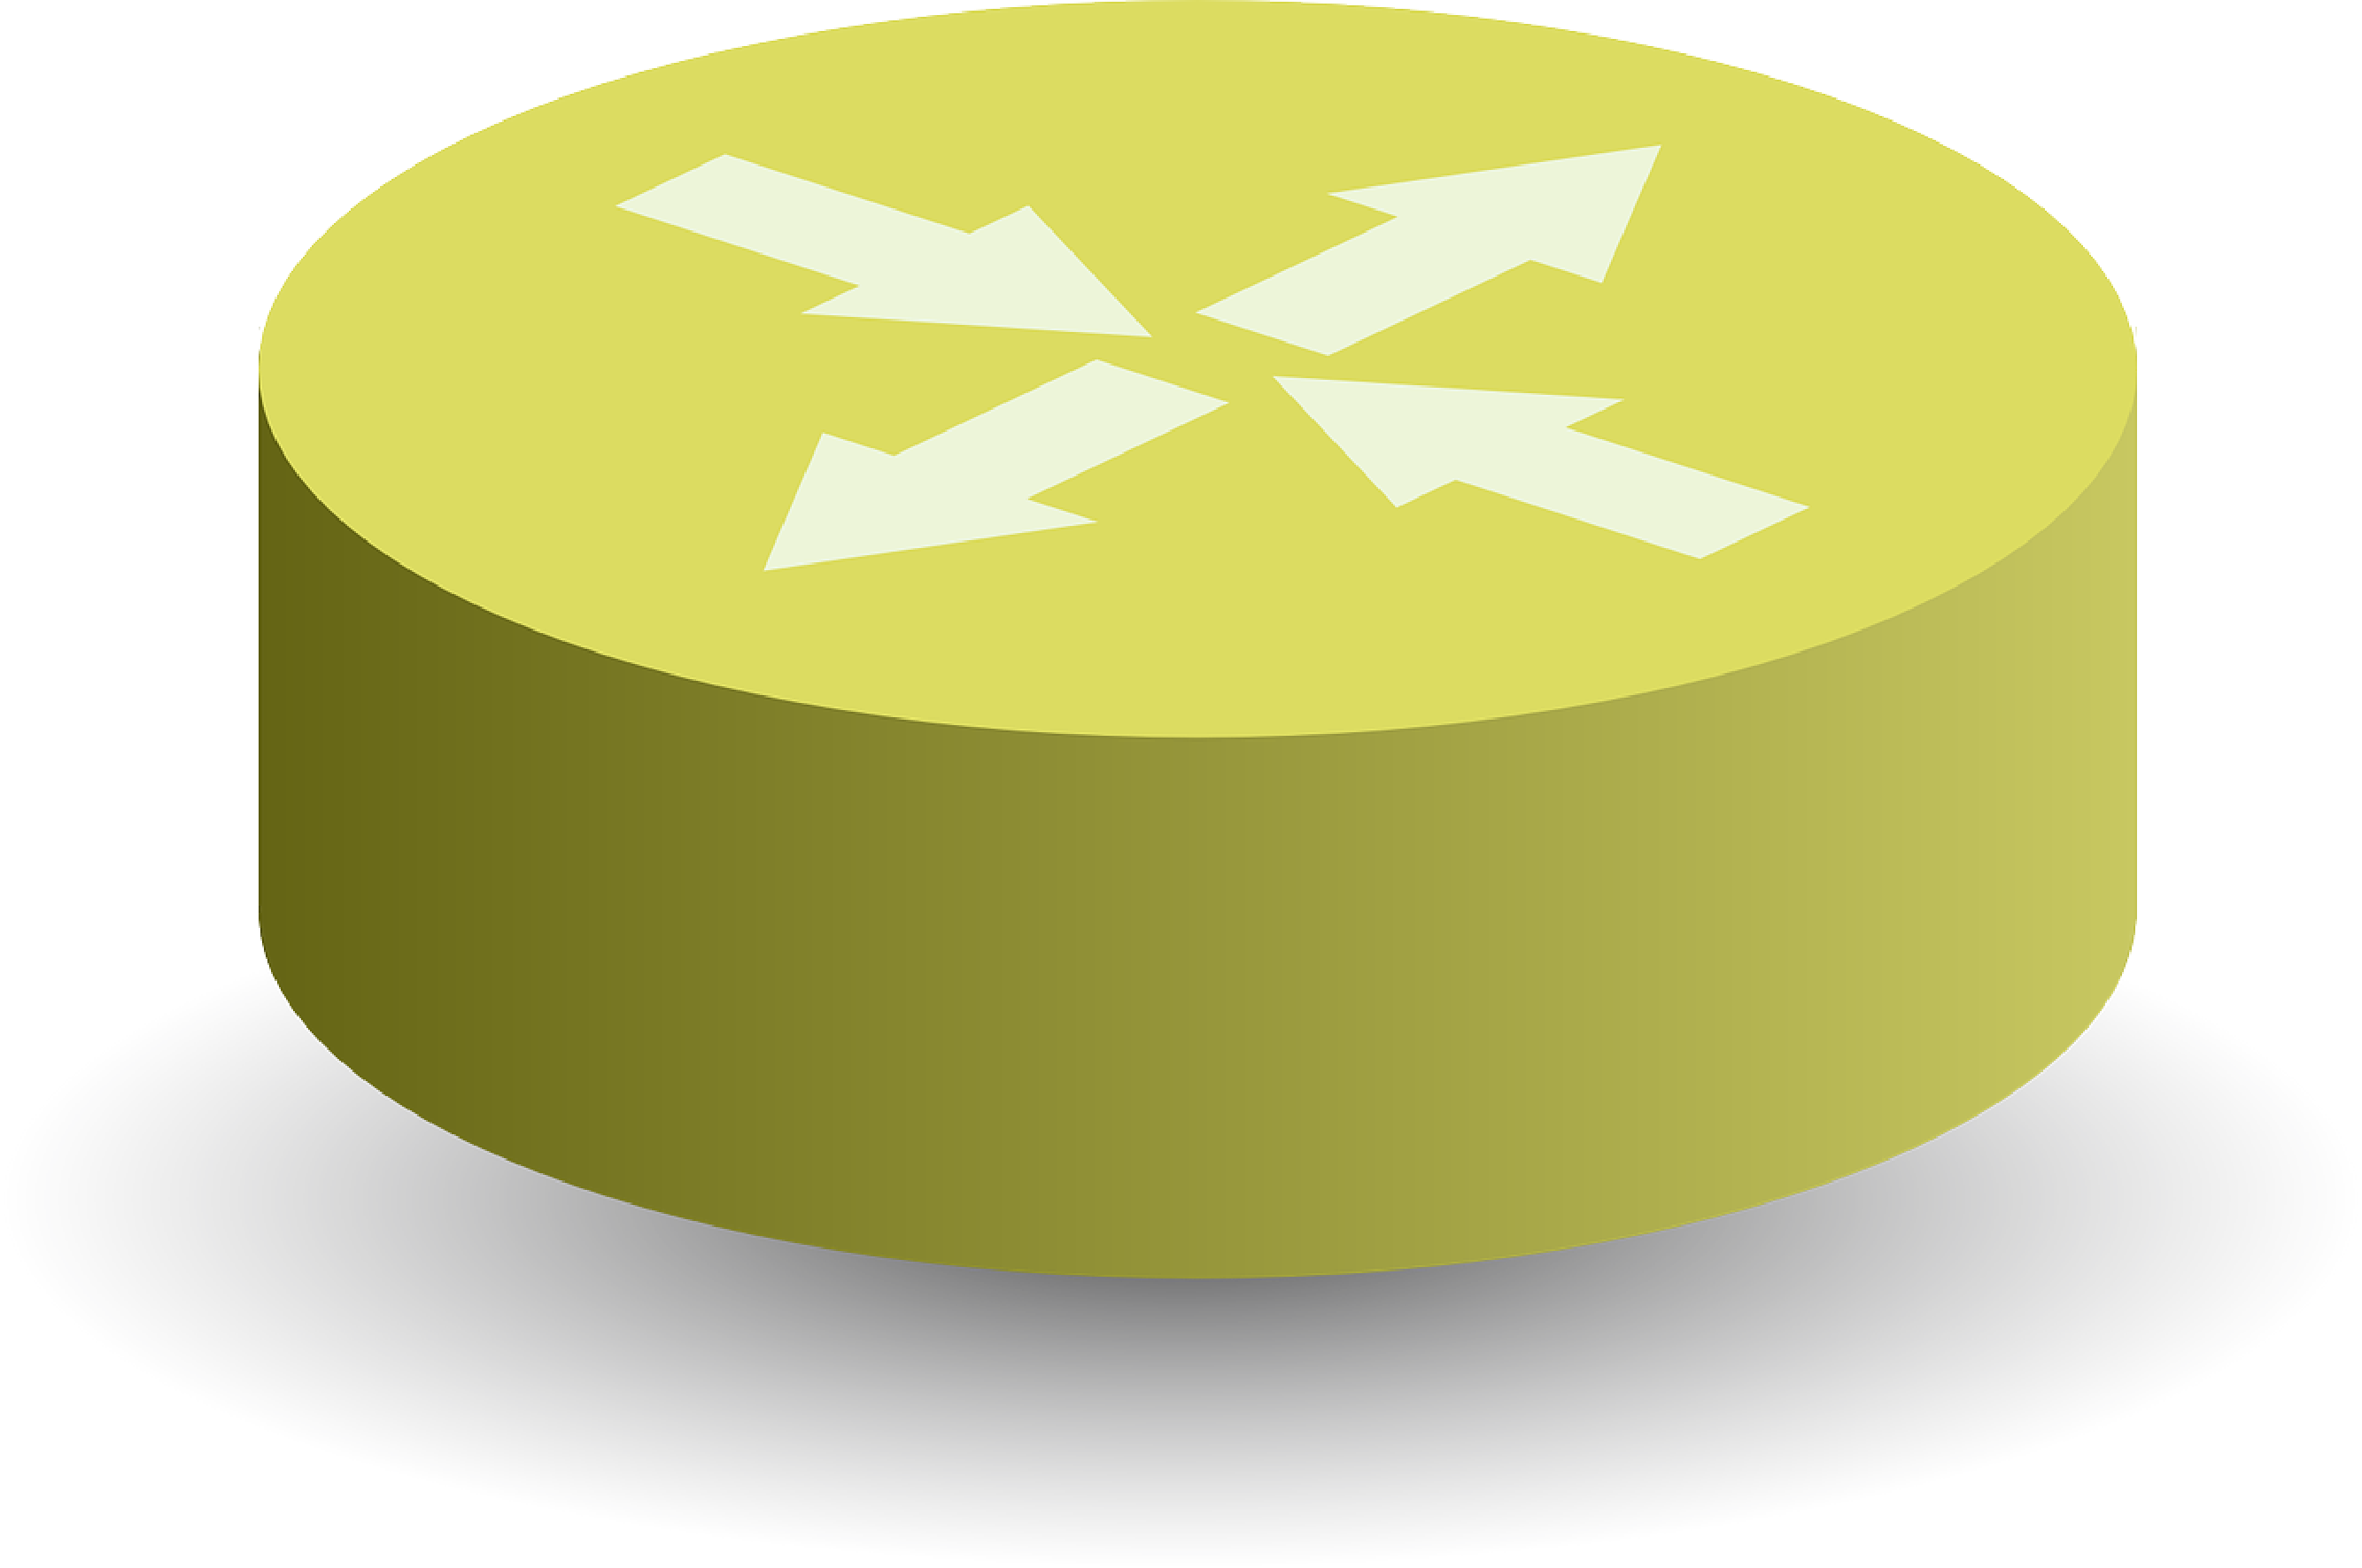
\includegraphics[width=52.5pt,height=52.5pt]{figures/router-158644_1280.pdf}};
%Image [id:dp04055959421826061] 
\draw (394.5,147.5) node  {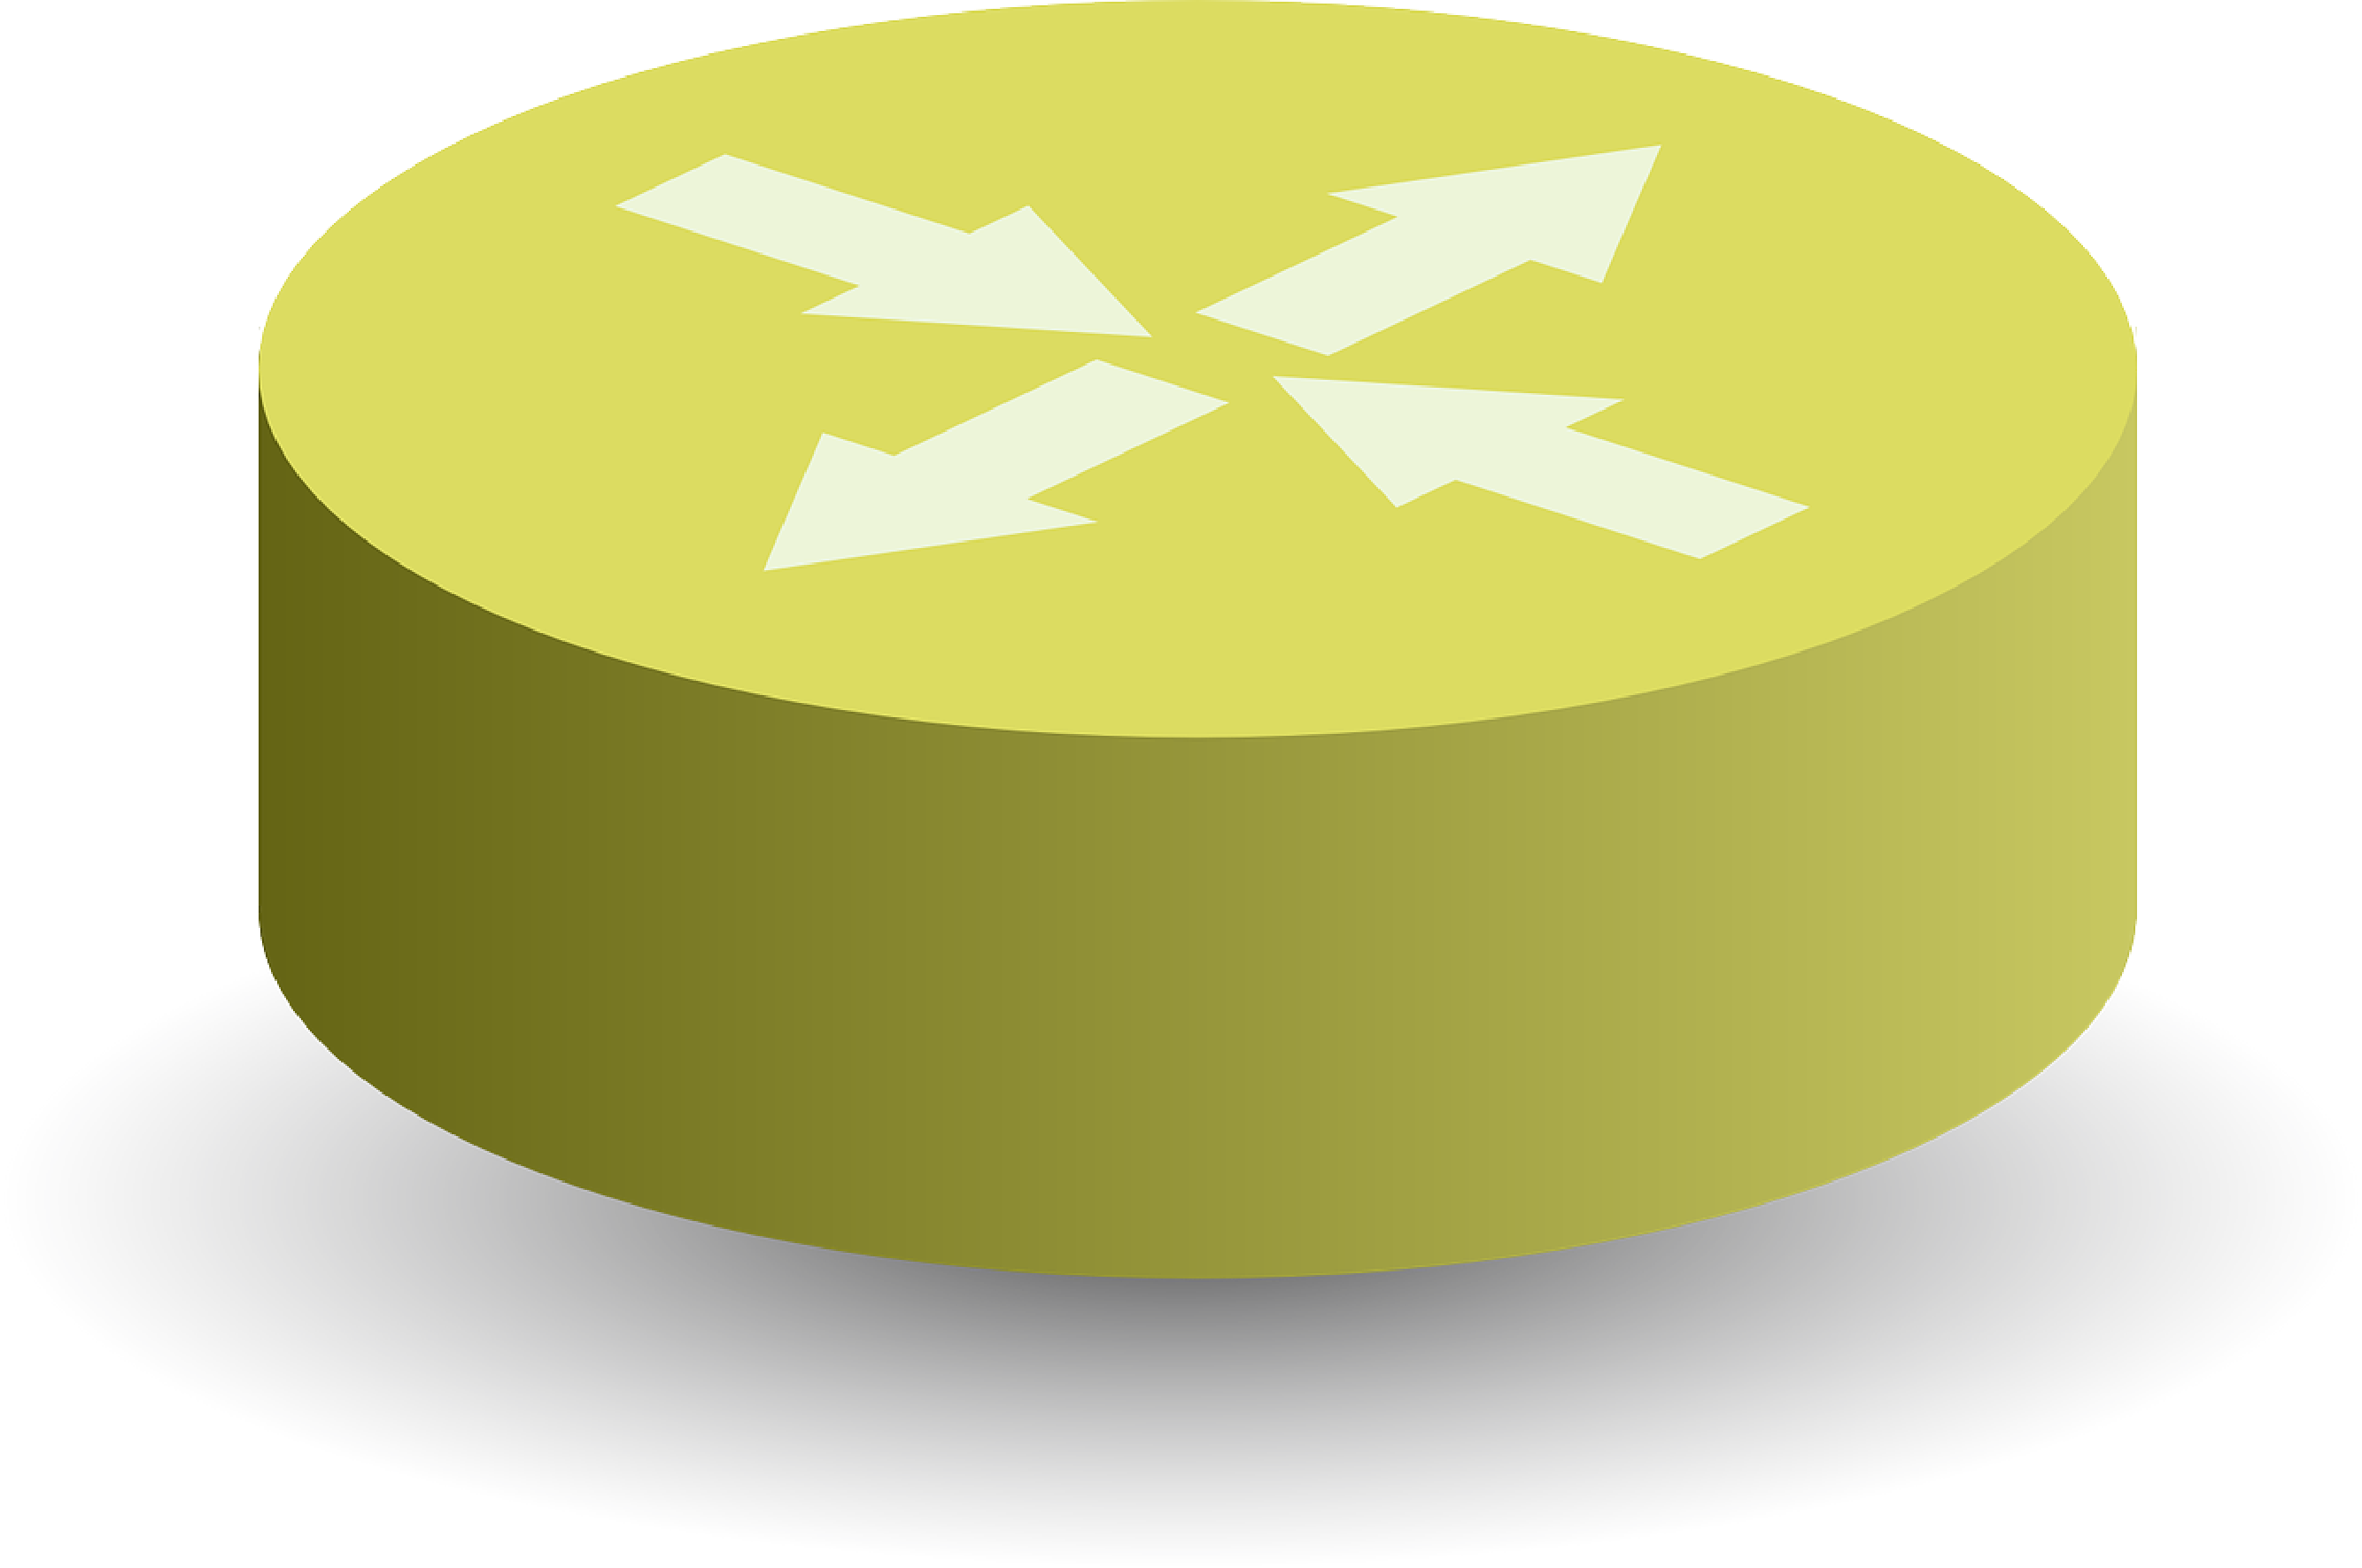
\includegraphics[width=52.5pt,height=52.5pt]{figures/router-158644_1280.pdf}};
%Image [id:dp9259427266230486] 
\draw (484,147.5) node  {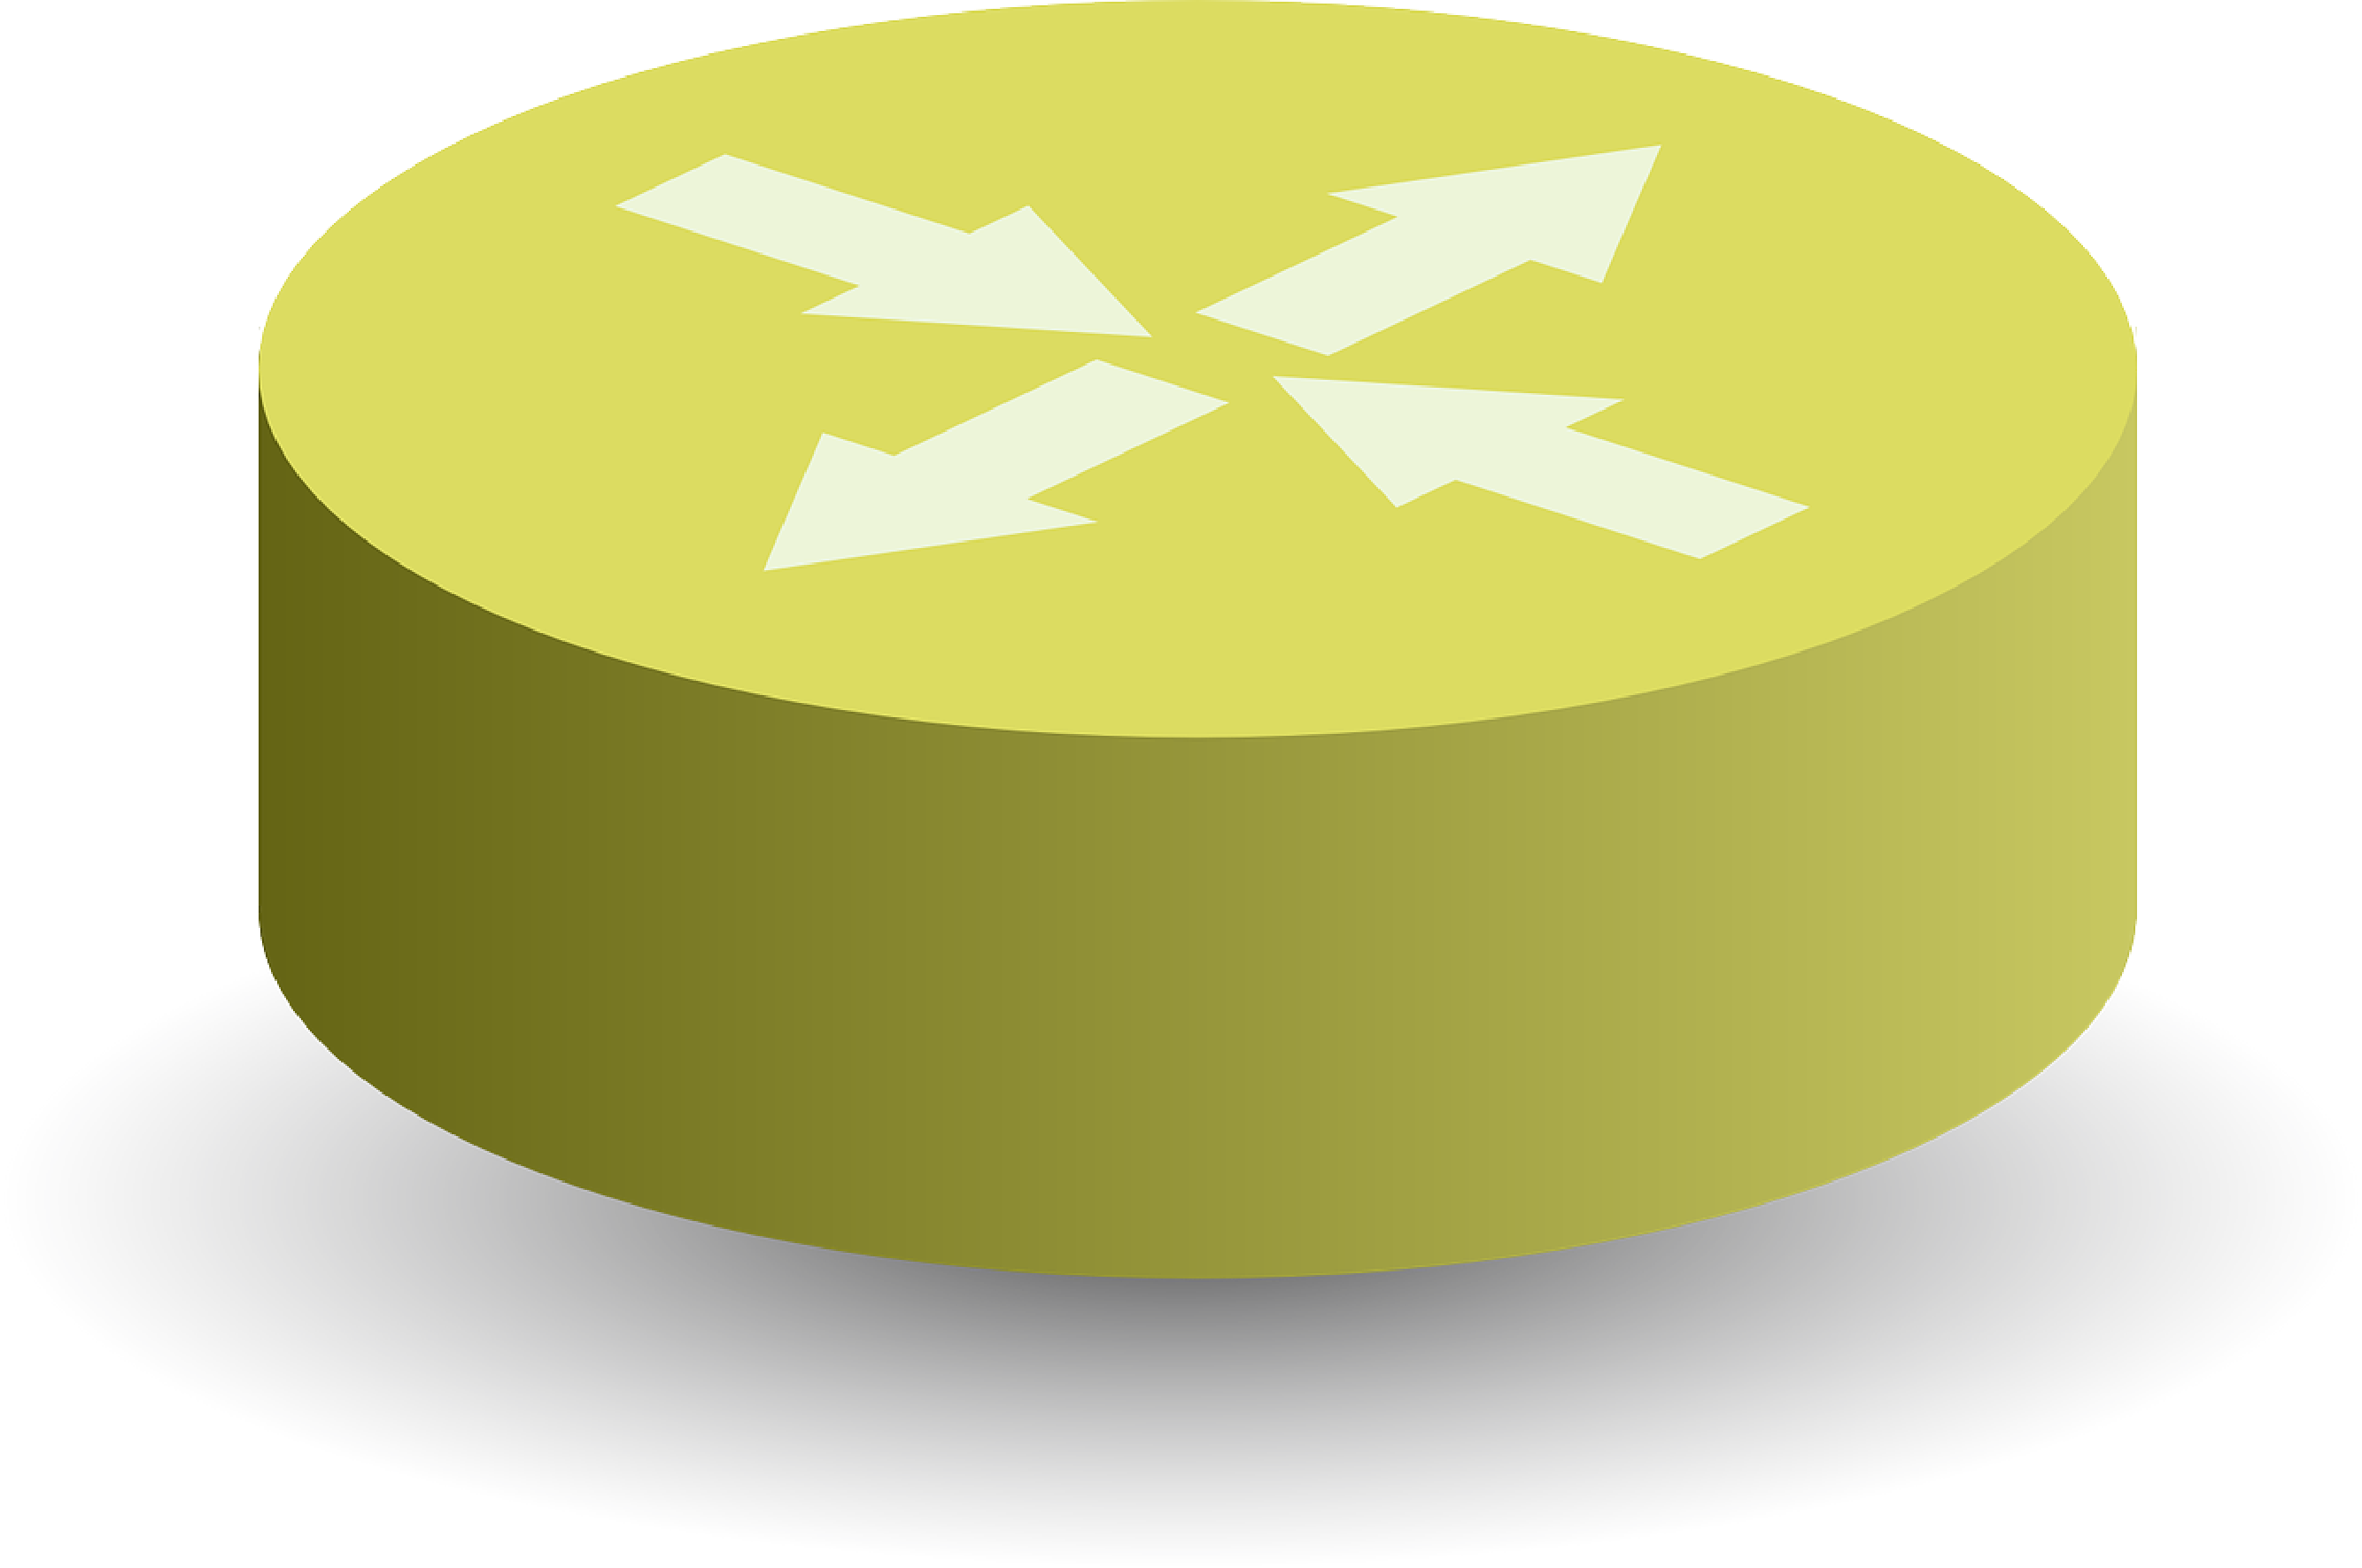
\includegraphics[width=52.5pt,height=52.5pt]{figures/router-158644_1280.pdf}};

%Rounded Rect [id:dp4478547267123999] 
\draw  [fill={rgb, 255:red, 255; green, 248; blue, 177 }  ,fill opacity=1 ] (26,125.27) .. controls (26,105.05) and (42.39,88.67) .. (62.6,88.67) -- (178.4,88.67) .. controls (198.61,88.67) and (215,105.05) .. (215,125.27) -- (215,235.07) .. controls (215,255.28) and (198.61,271.67) .. (178.4,271.67) -- (62.6,271.67) .. controls (42.39,271.67) and (26,255.28) .. (26,235.07) -- cycle ;
%Straight Lines [id:da04812807065340363] 
\draw    (56,180.67) -- (166,134.67) ;


%Image [id:dp341968705695737] 
\draw (61,184.5) node  {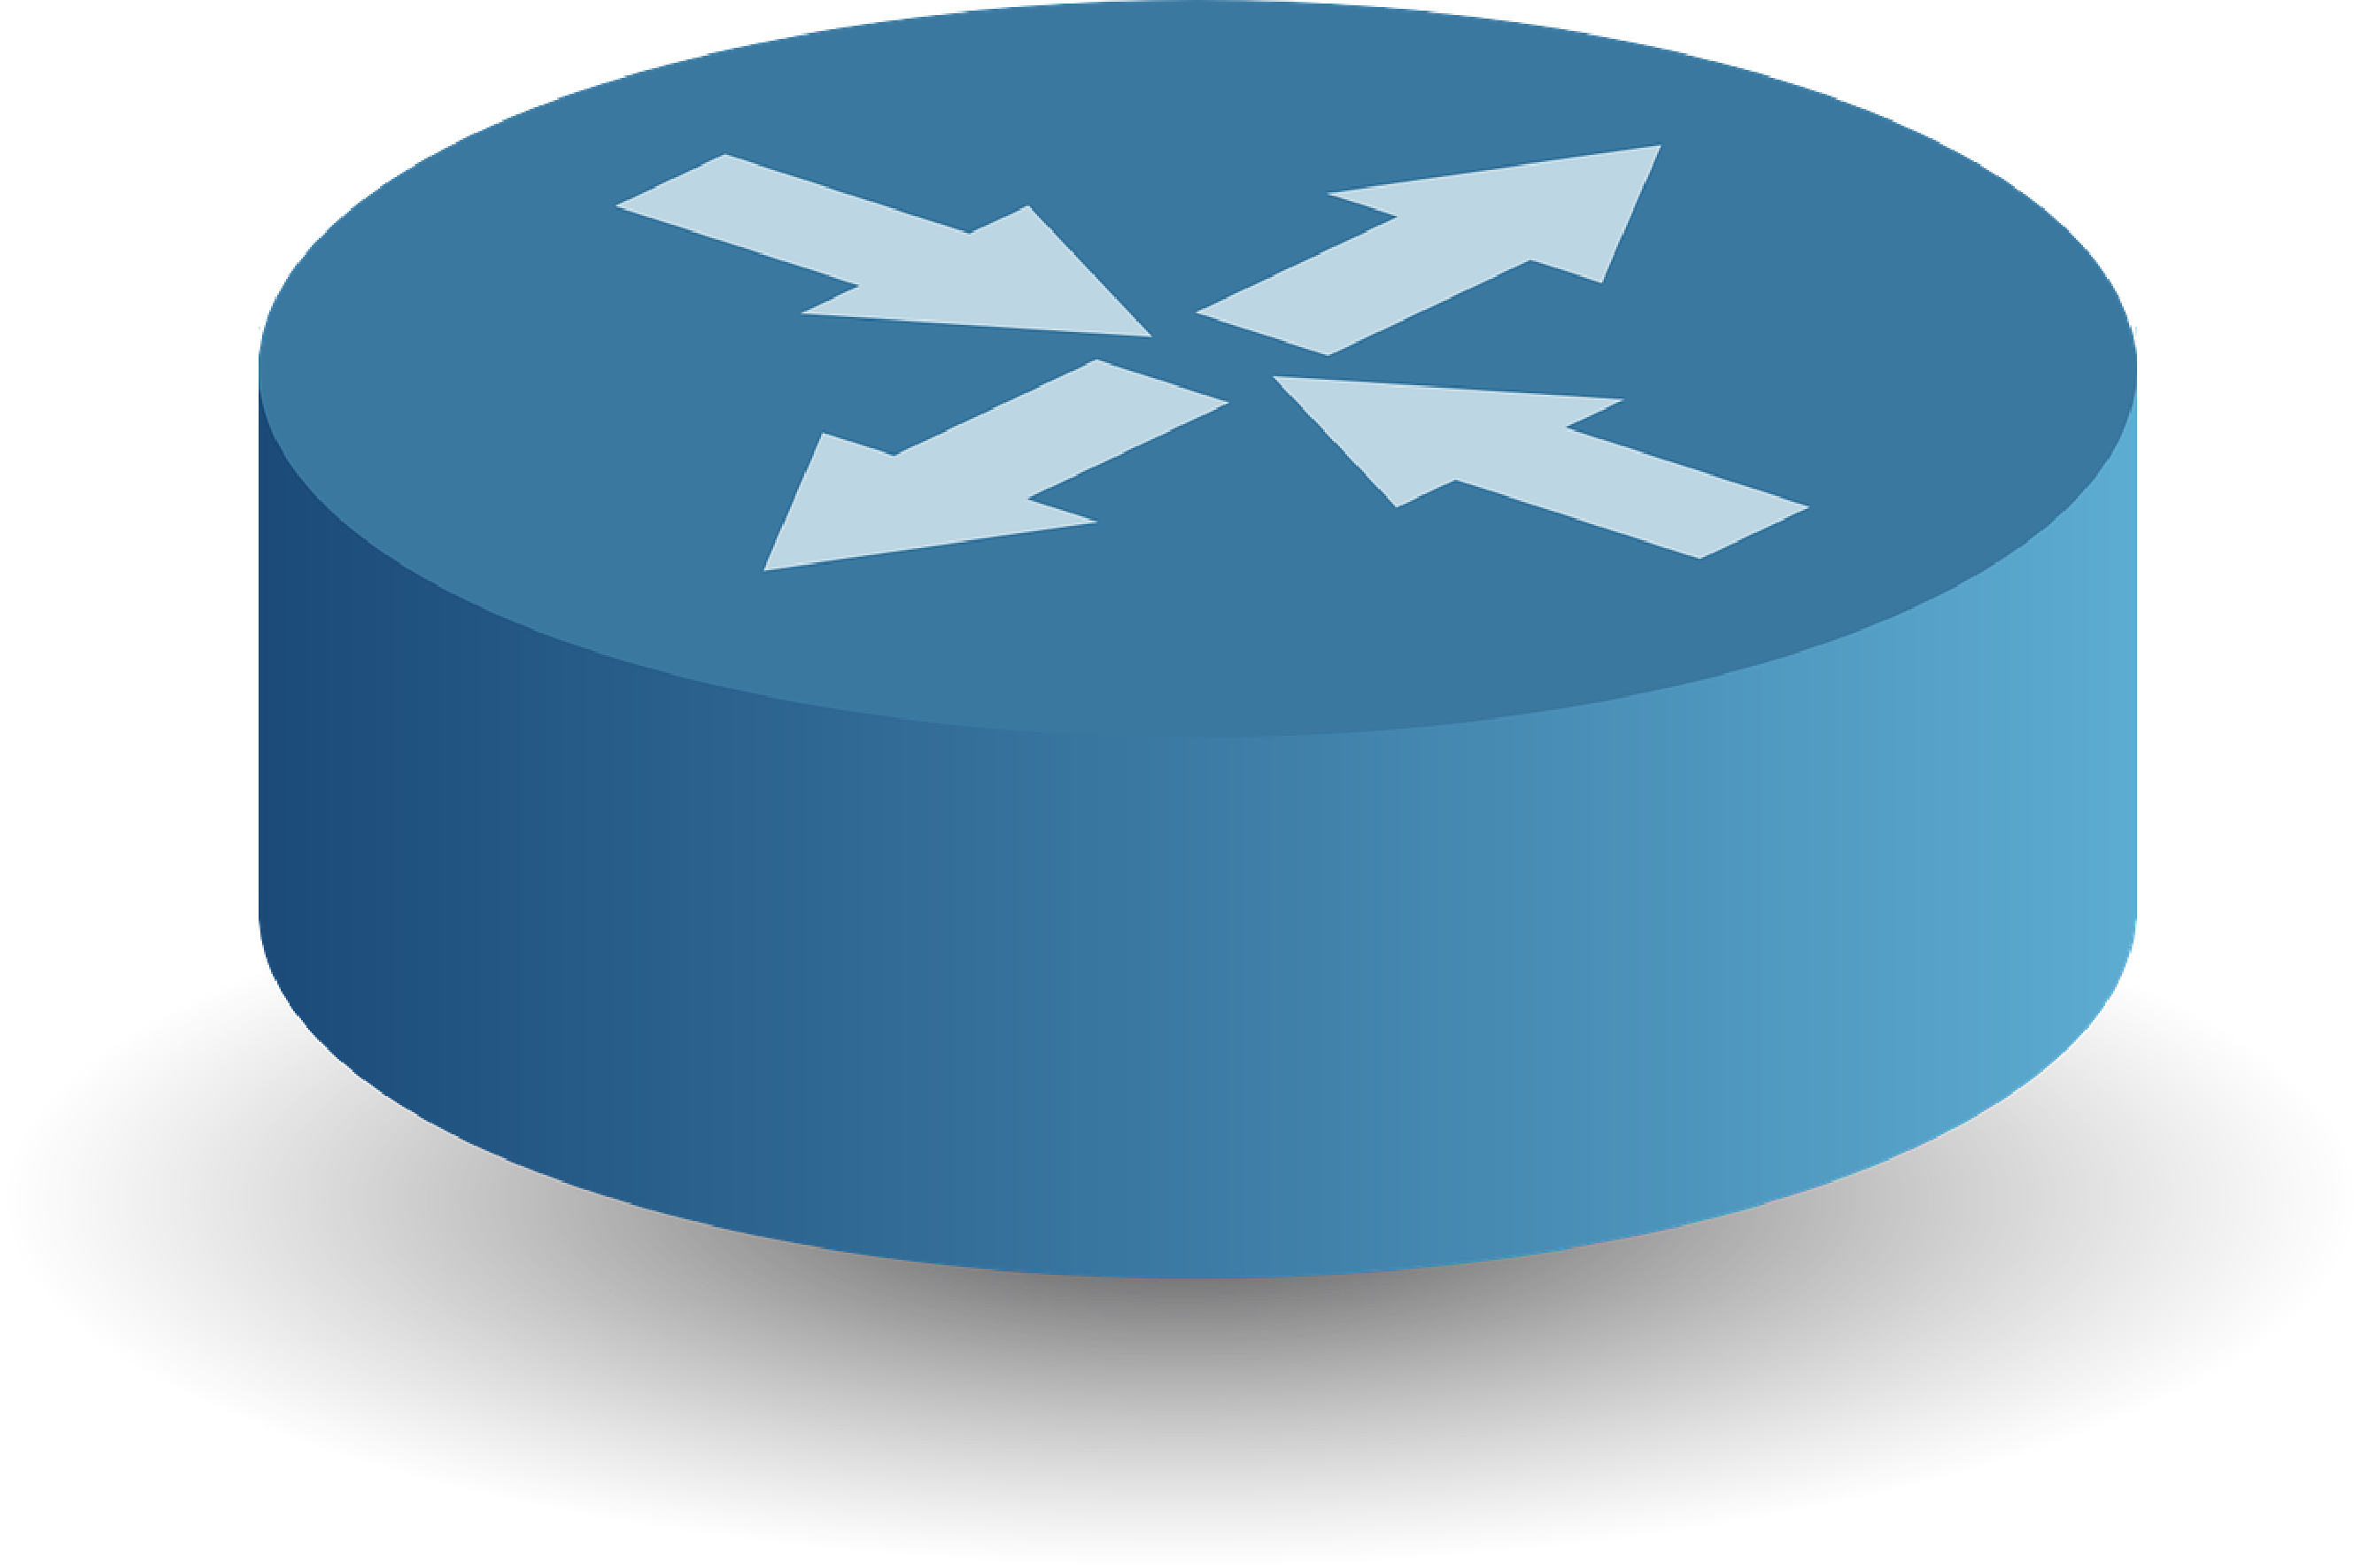
\includegraphics[width=52.5pt,height=52.5pt]{figures/router-29825_1280.pdf}};
%Image [id:dp7725023918834623] 
\draw (165,130.5) node  {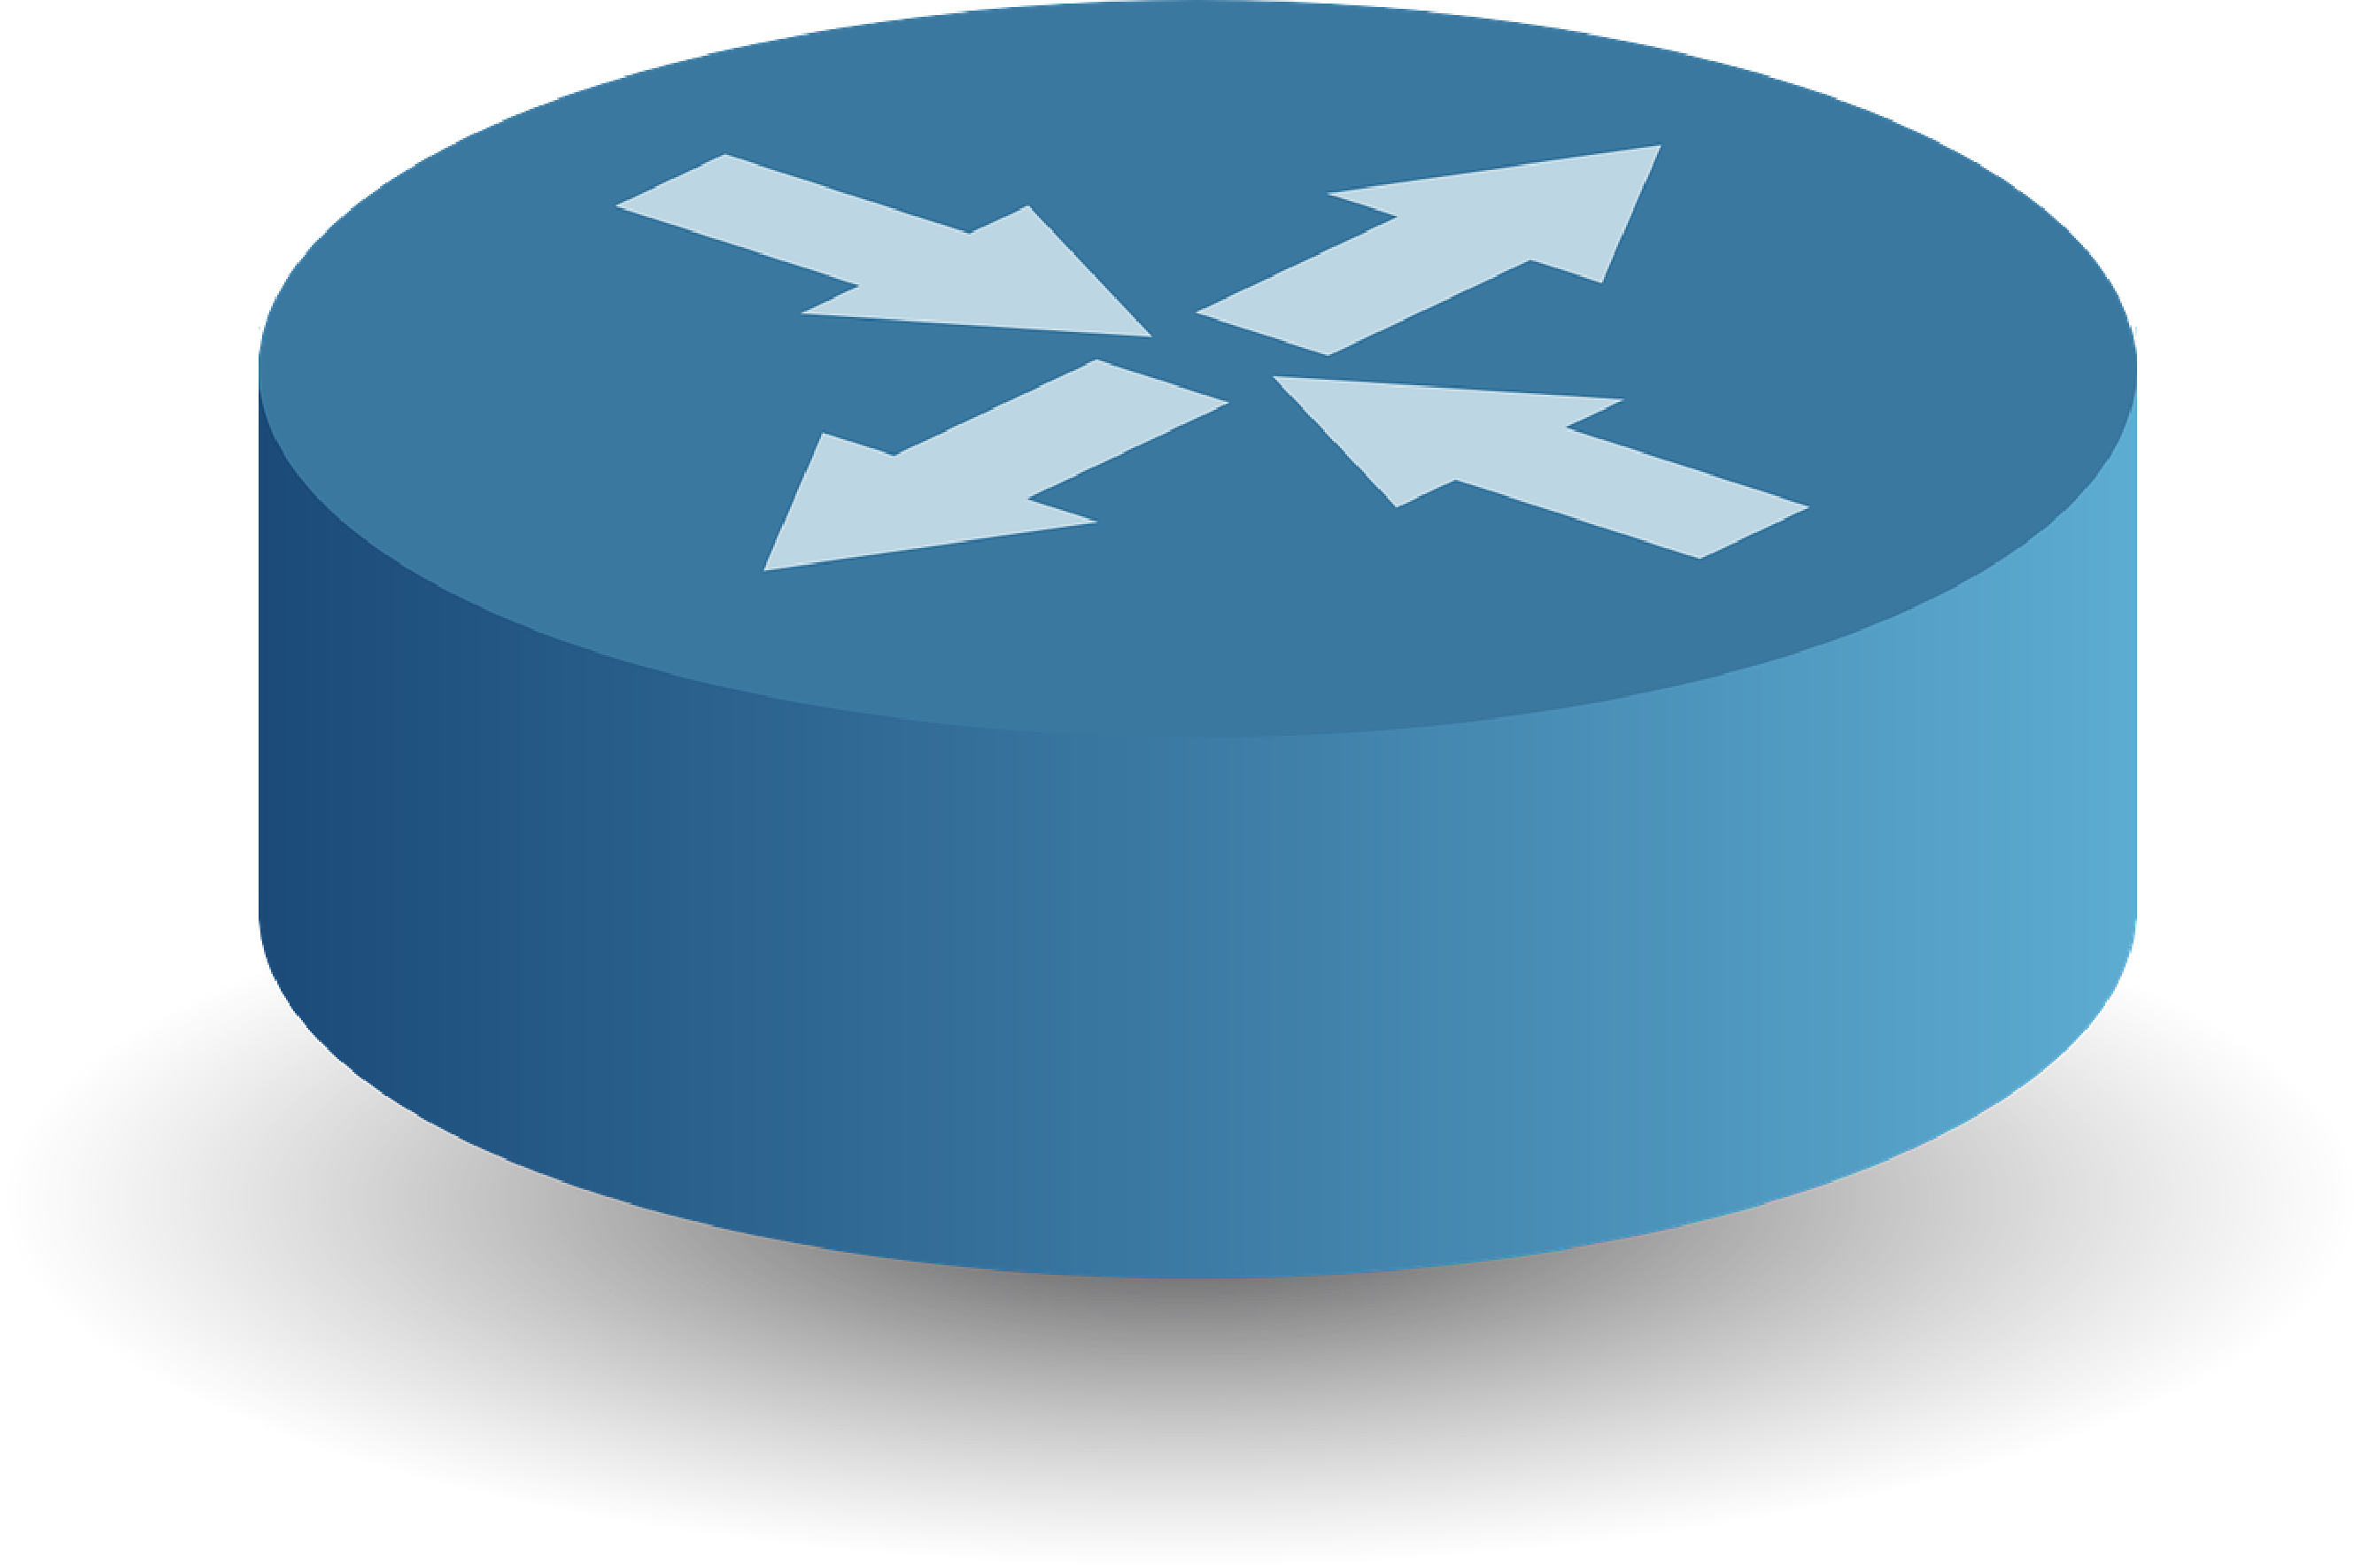
\includegraphics[width=52.5pt,height=52.5pt]{figures/router-29825_1280.pdf}};

%Straight Lines [id:da036026819015278266] 
\draw    (81,200.17) -- (138,225.67) ;


%Image [id:dp29149867233304716] 
\draw (136,238.5) node  {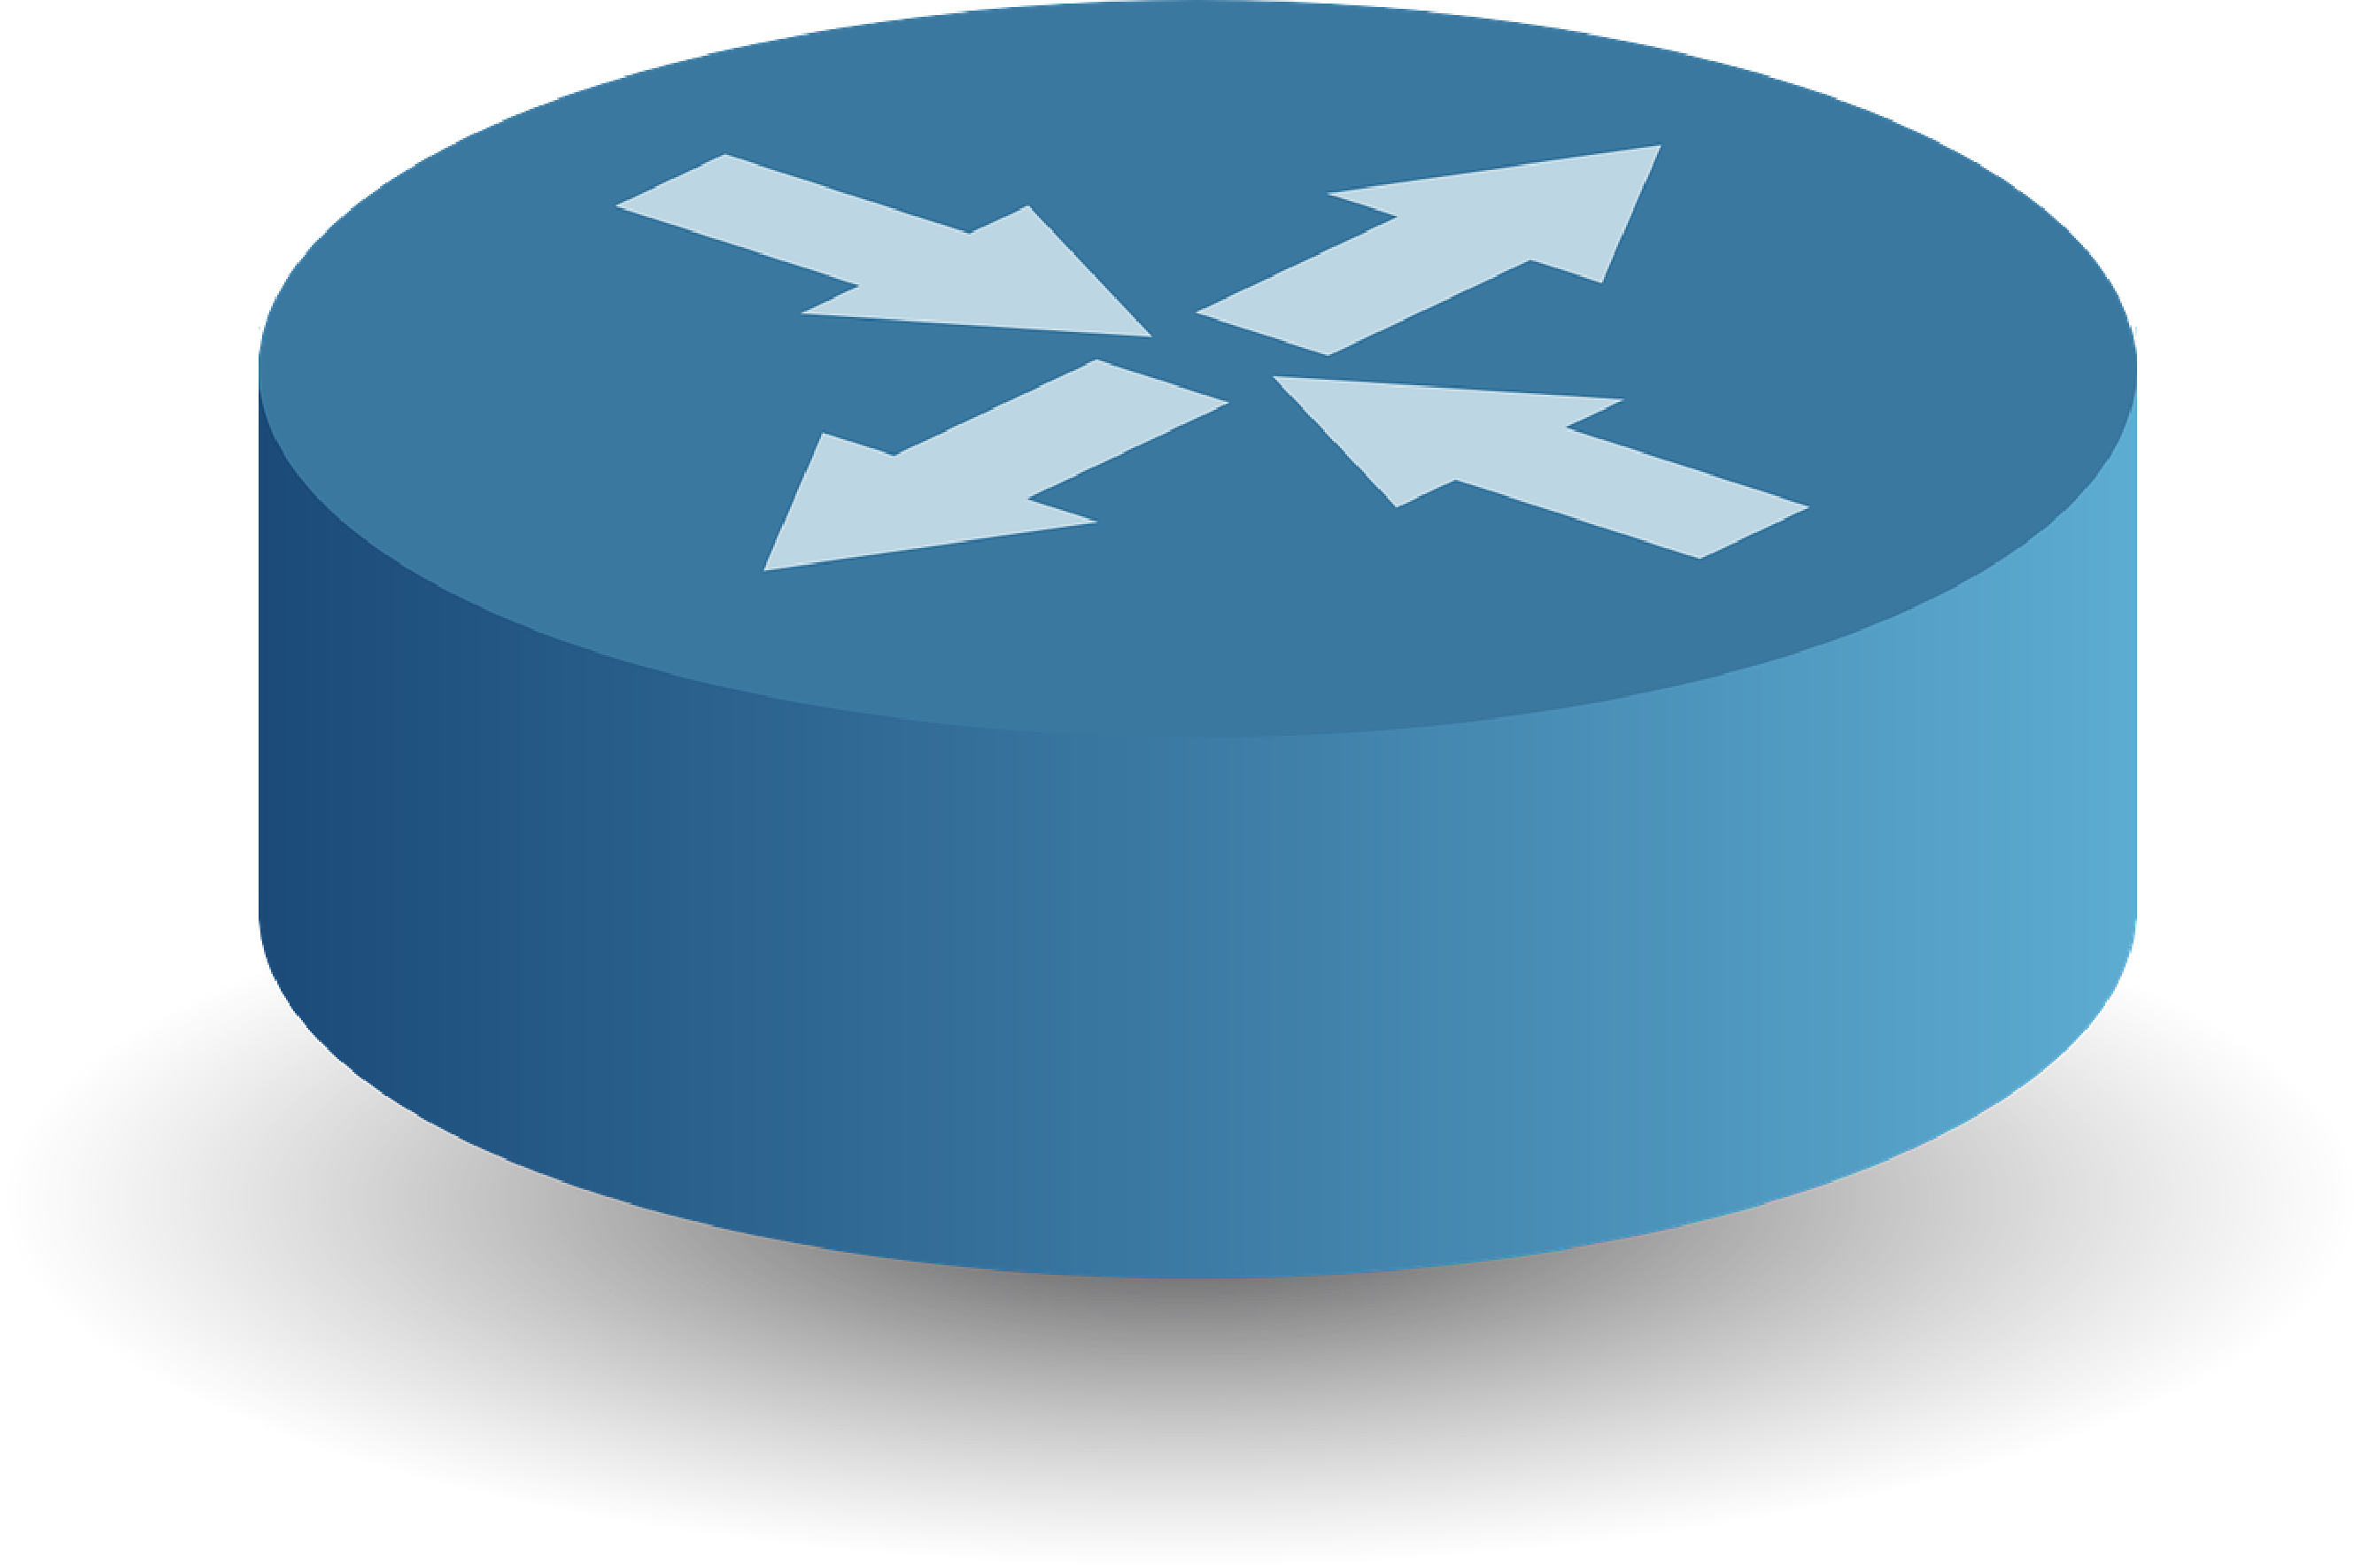
\includegraphics[width=52.5pt,height=52.5pt]{figures/router-29825_1280.pdf}};

%Rounded Rect [id:dp8669891034149613] 
\draw  [fill={rgb, 255:red, 184; green, 233; blue, 134 }  ,fill opacity=1 ] (8,398.47) .. controls (8,383.11) and (20.45,370.67) .. (35.8,370.67) -- (583.2,370.67) .. controls (598.55,370.67) and (611,383.11) .. (611,398.47) -- (611,481.87) .. controls (611,497.22) and (598.55,509.67) .. (583.2,509.67) -- (35.8,509.67) .. controls (20.45,509.67) and (8,497.22) .. (8,481.87) -- cycle ;
%Straight Lines [id:da7257050611297167] 
\draw    (79,428.67) -- (214,401.67) ;


%Straight Lines [id:da6984840894149047] 
\draw    (80,443.67) -- (171,466.67) ;


%Straight Lines [id:da6802535311385733] 
\draw    (174,473.67) -- (368,426.67) ;


%Straight Lines [id:da14214857377238777] 
\draw    (214,401.67) -- (358,410.67) ;


%Straight Lines [id:da6556428261701027] 
\draw    (384,420.67) -- (502,407.67) ;


%Straight Lines [id:da16066583484396146] 
\draw    (375,440.67) -- (477,476.67) ;


%Image [id:dp1703433460369157] 
\draw (70,443.5) node  {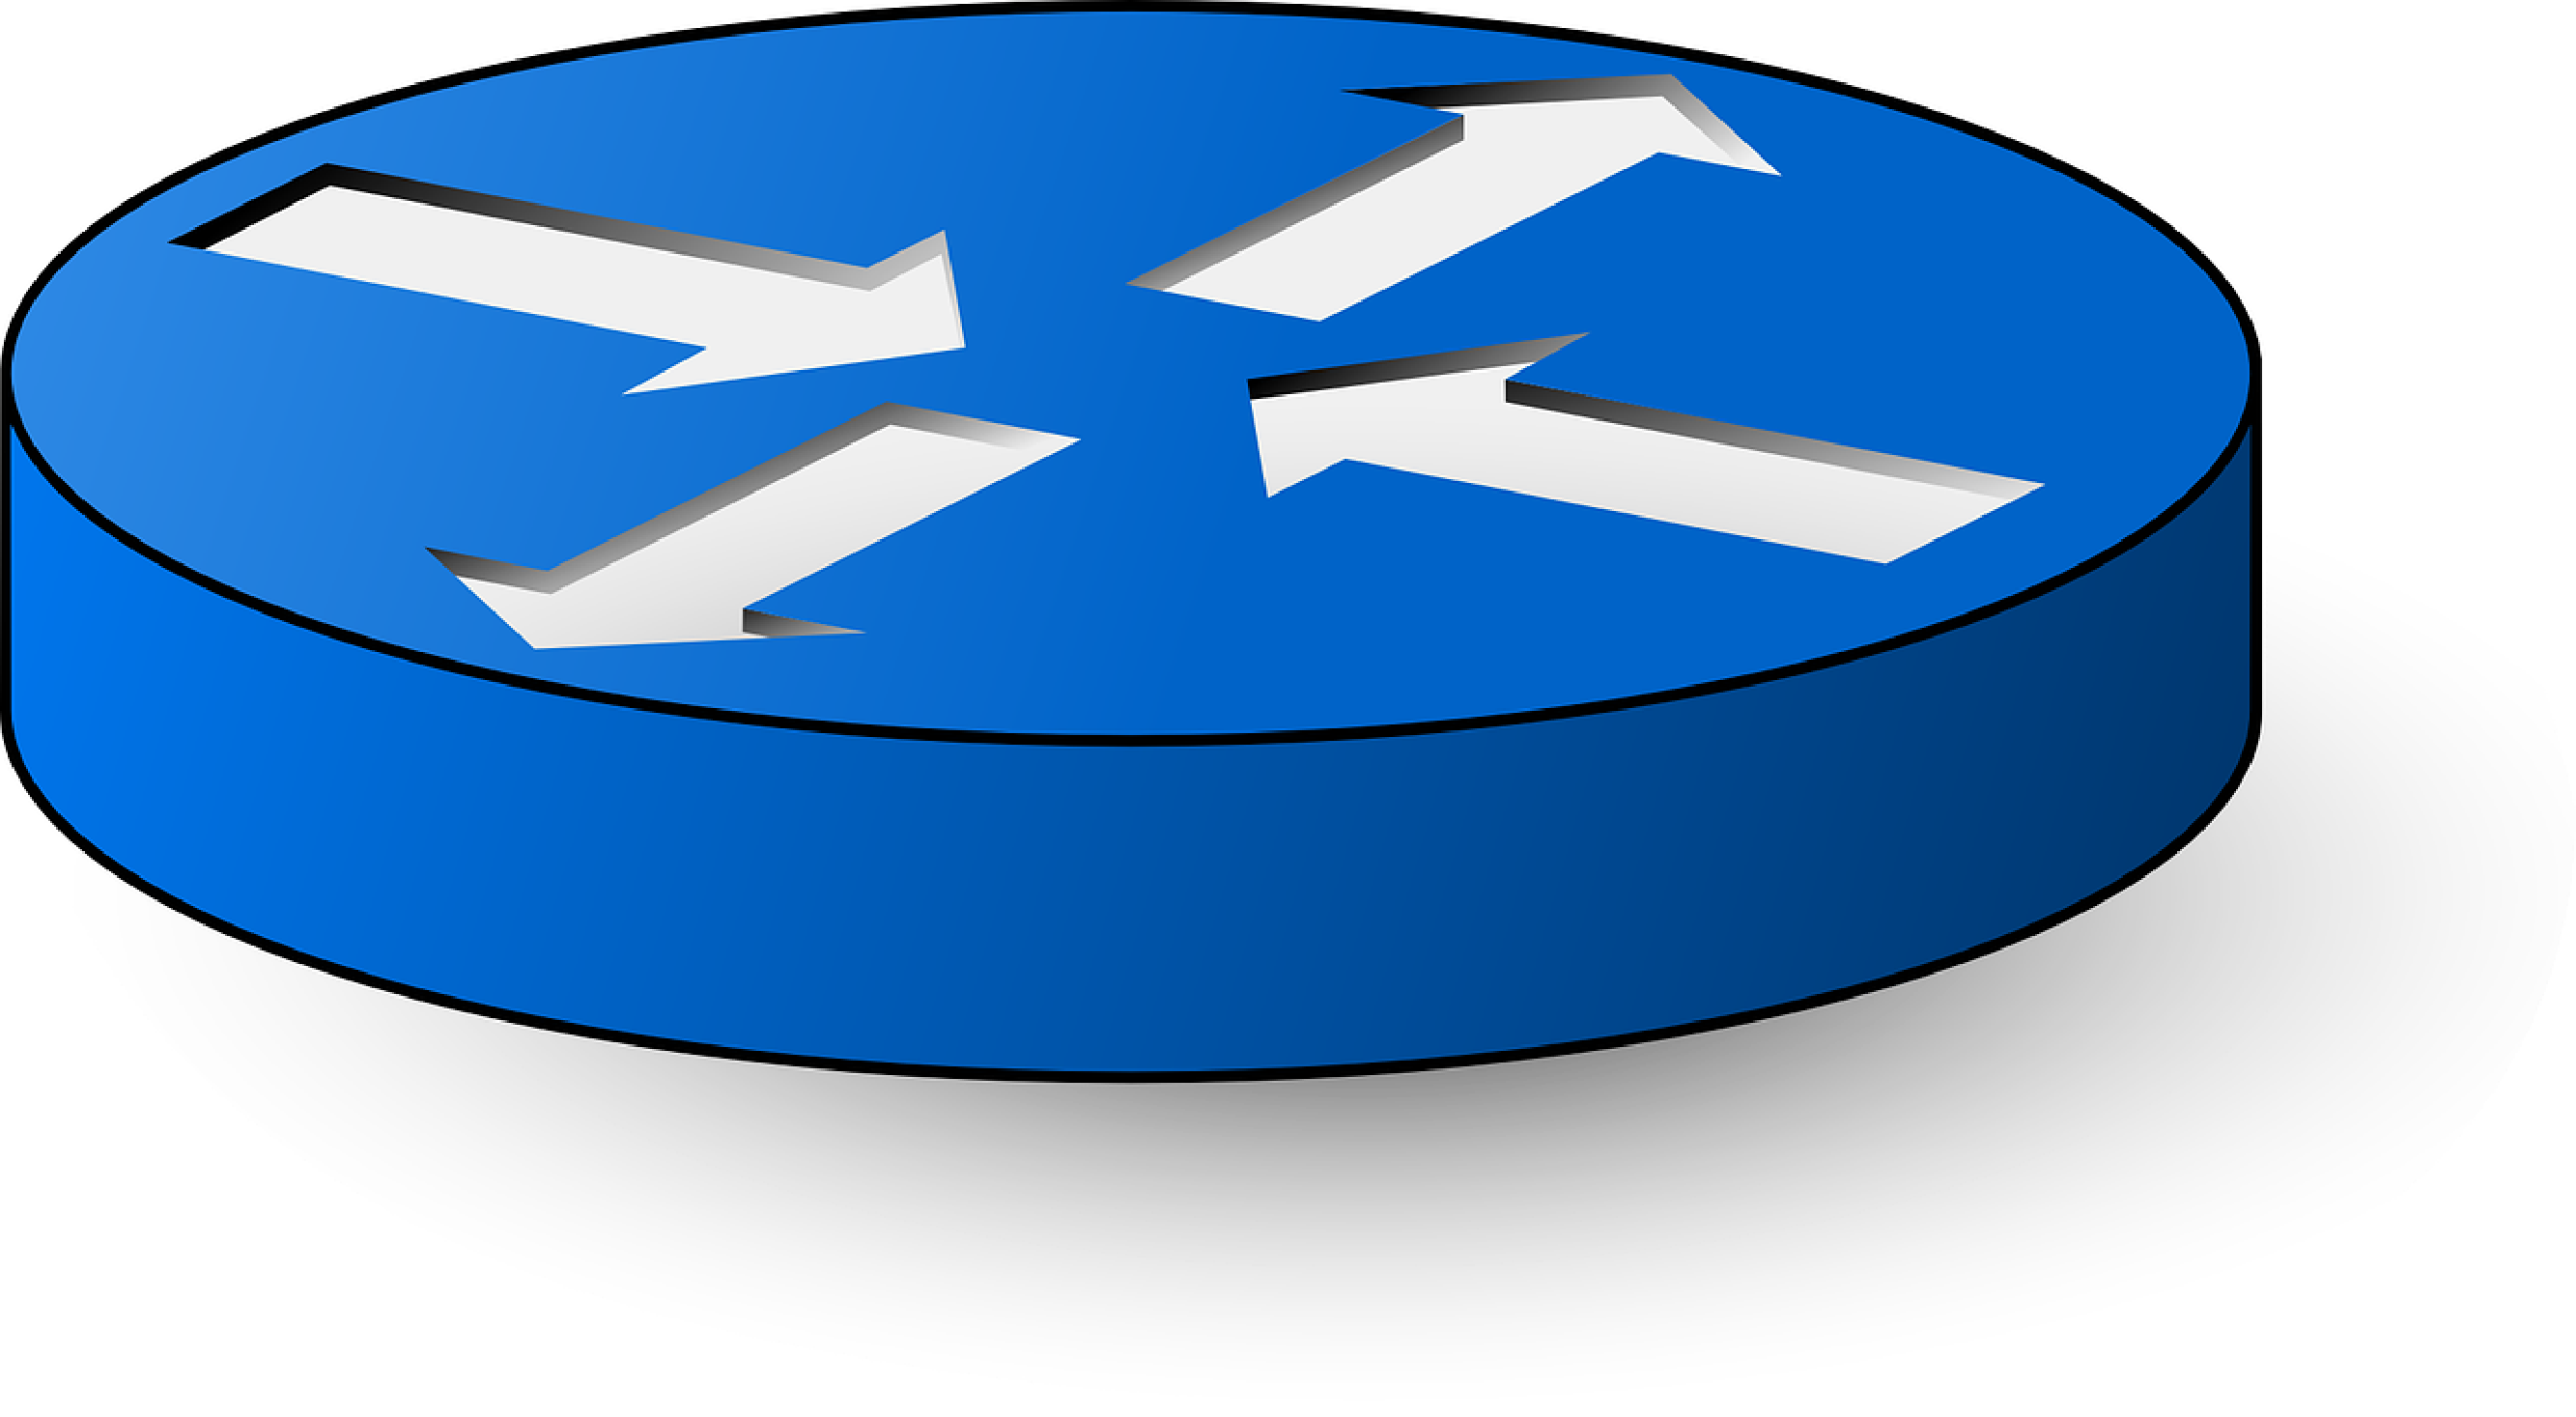
\includegraphics[width=52.5pt,height=52.5pt]{figures/router-30140_1280.pdf}};
%Image [id:dp7119657242561229] 
\draw (160,474.5) node  {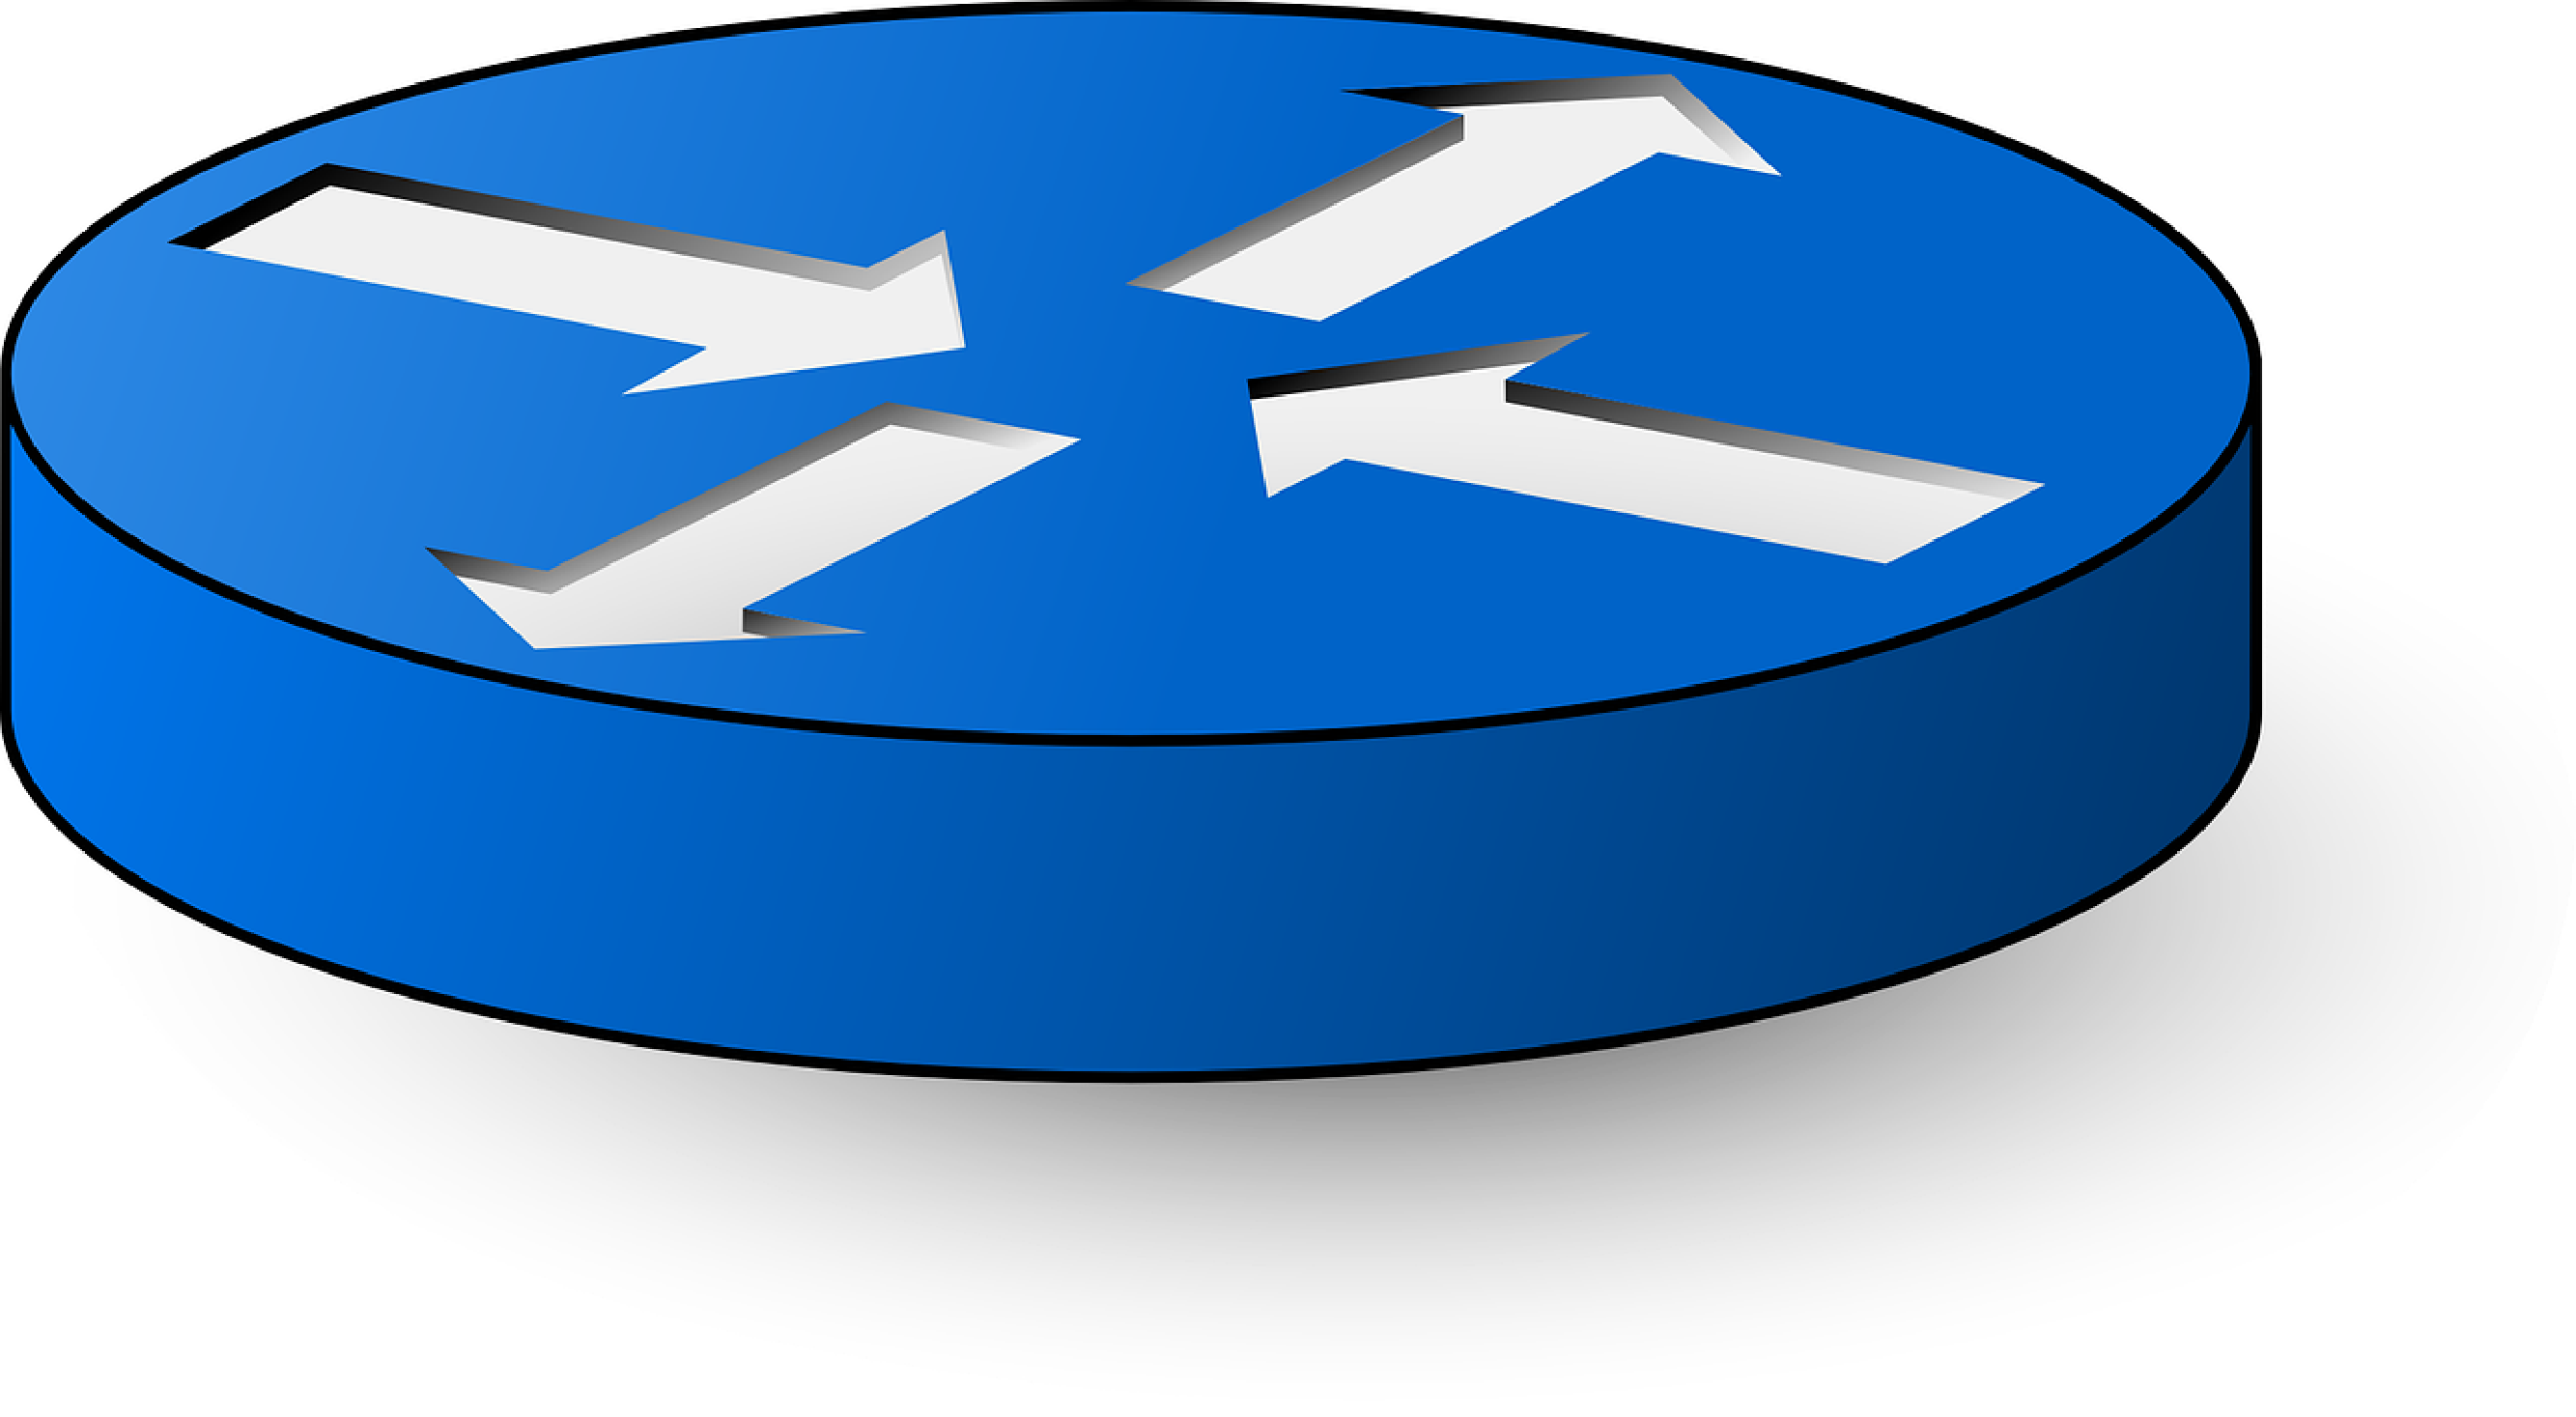
\includegraphics[width=52.5pt,height=52.5pt]{figures/router-30140_1280.pdf}};
%Image [id:dp01793726972424281] 
\draw (200,411.5) node  {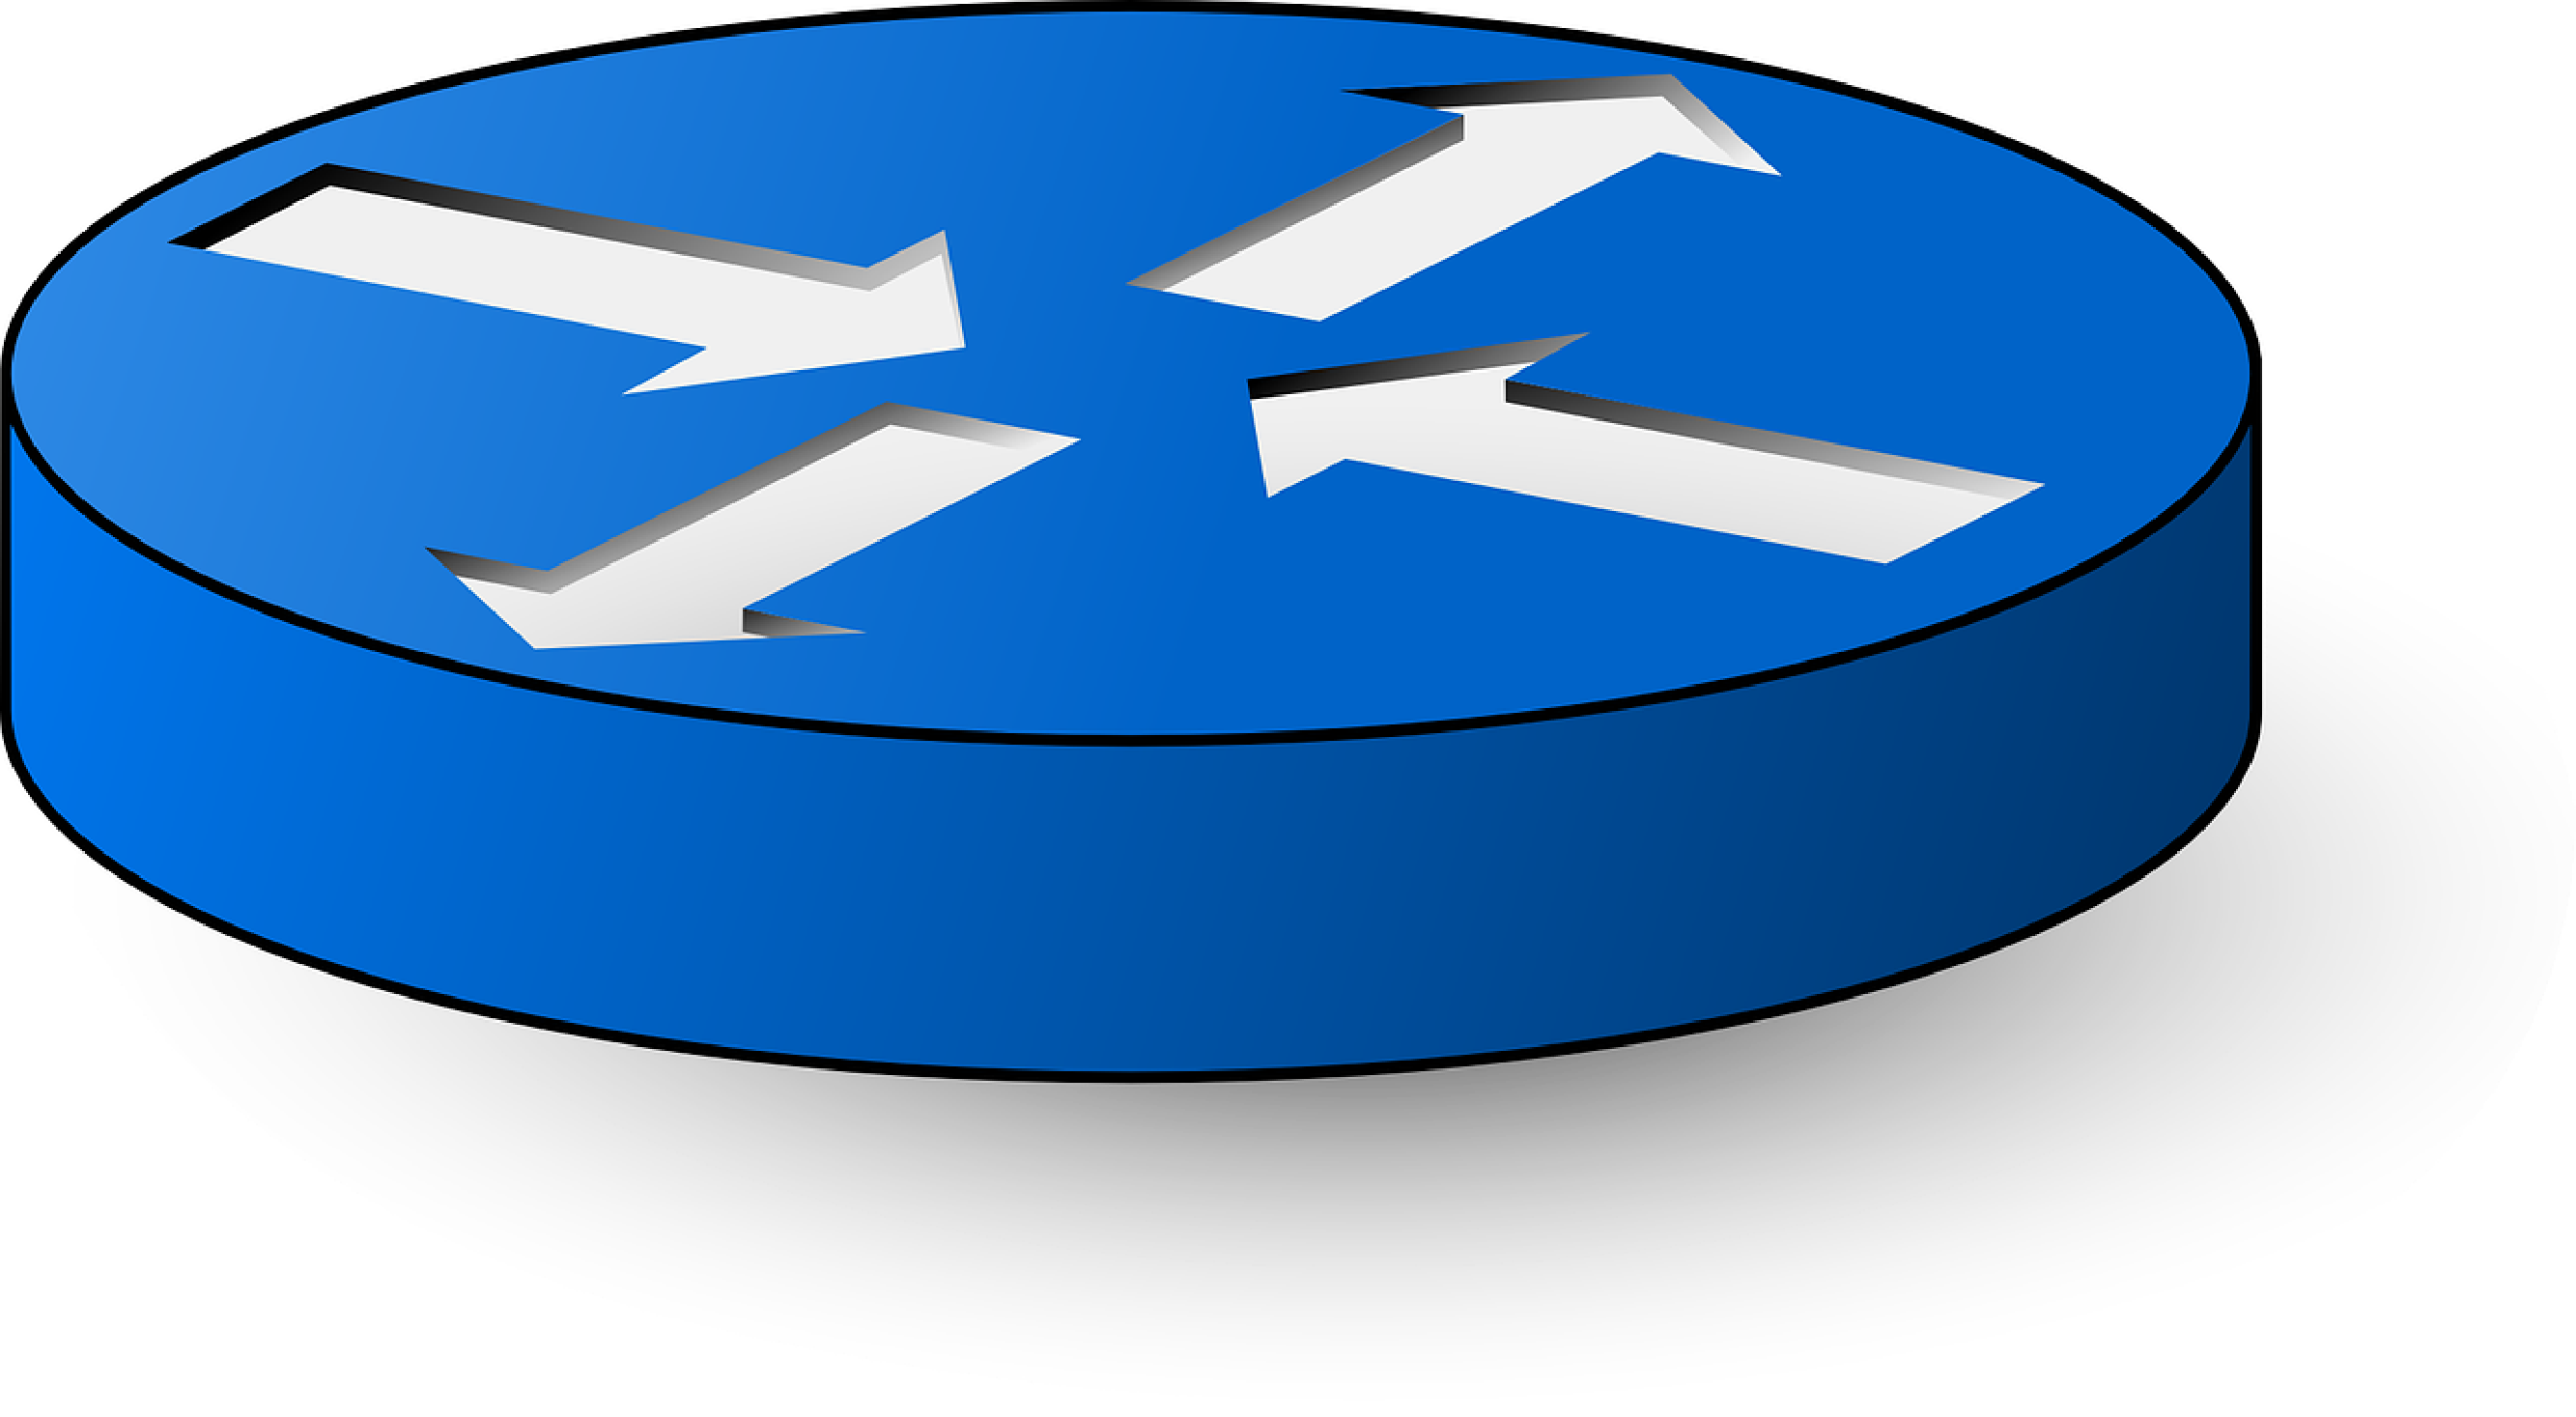
\includegraphics[width=52.5pt,height=52.5pt]{figures/router-30140_1280.pdf}};
%Image [id:dp9361502418924952] 
\draw (386,425.5) node  {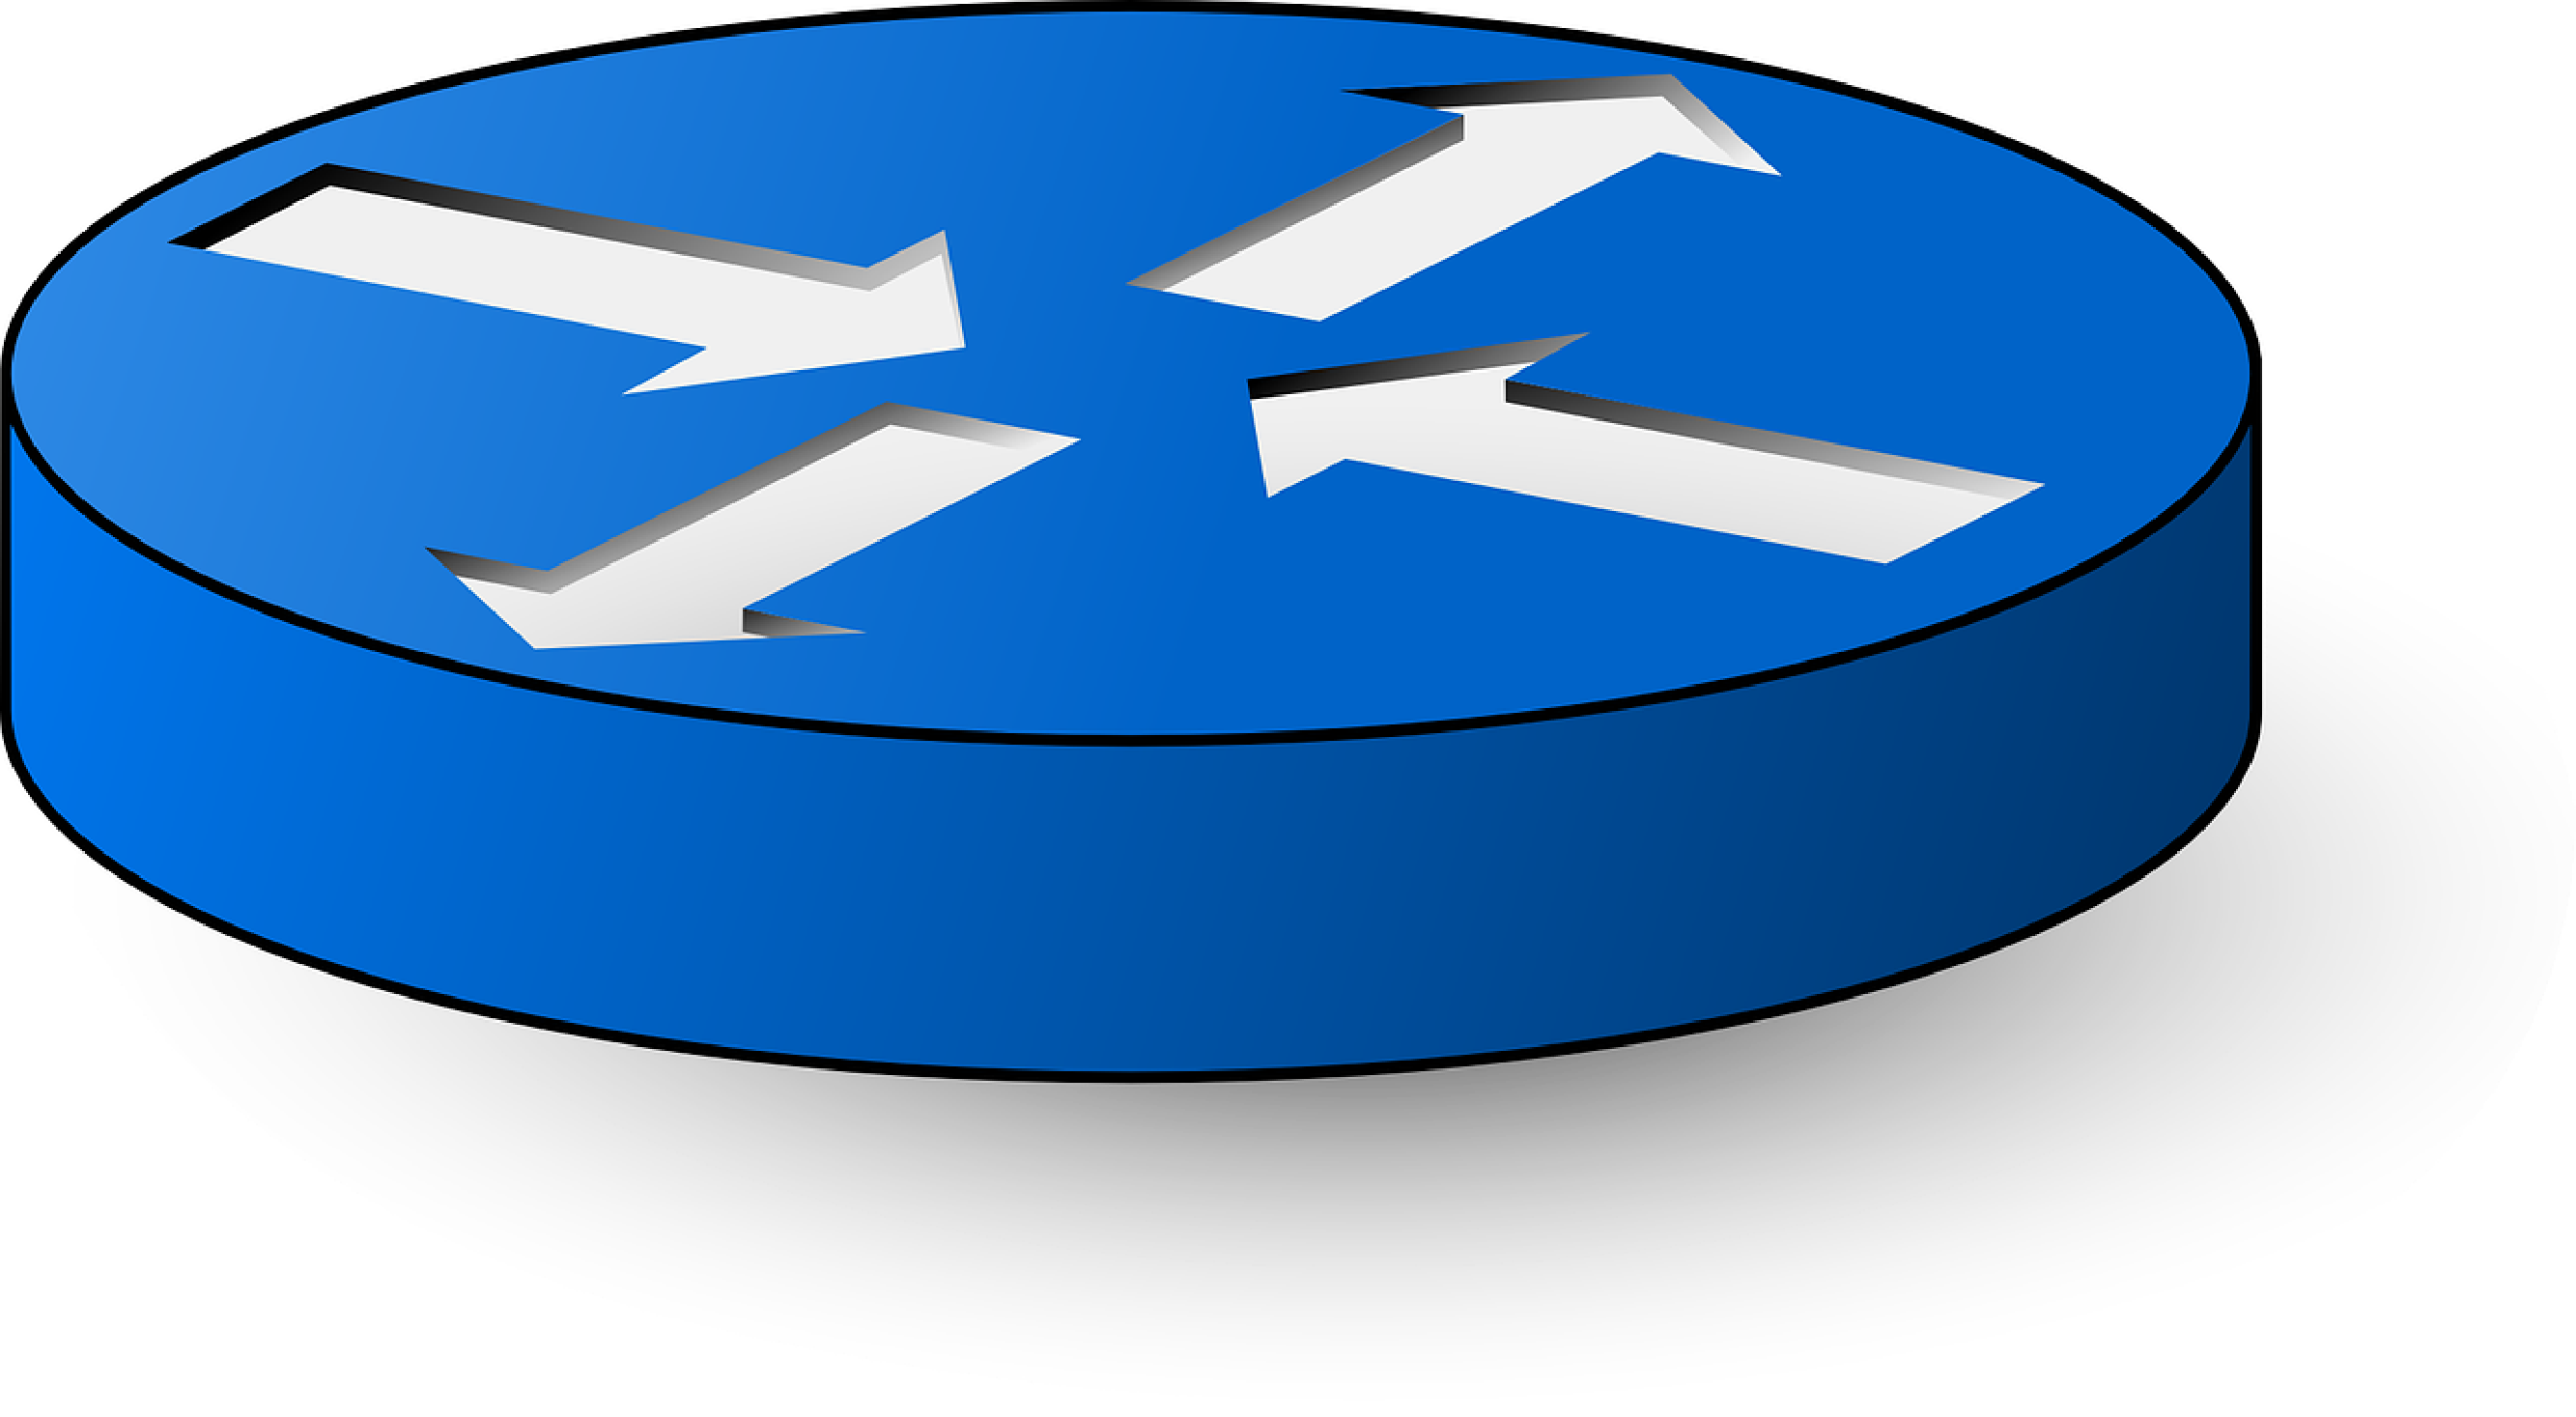
\includegraphics[width=52.5pt,height=52.5pt]{figures/router-30140_1280.pdf}};
%Image [id:dp1834582453825948] 
\draw (515,414.5) node  {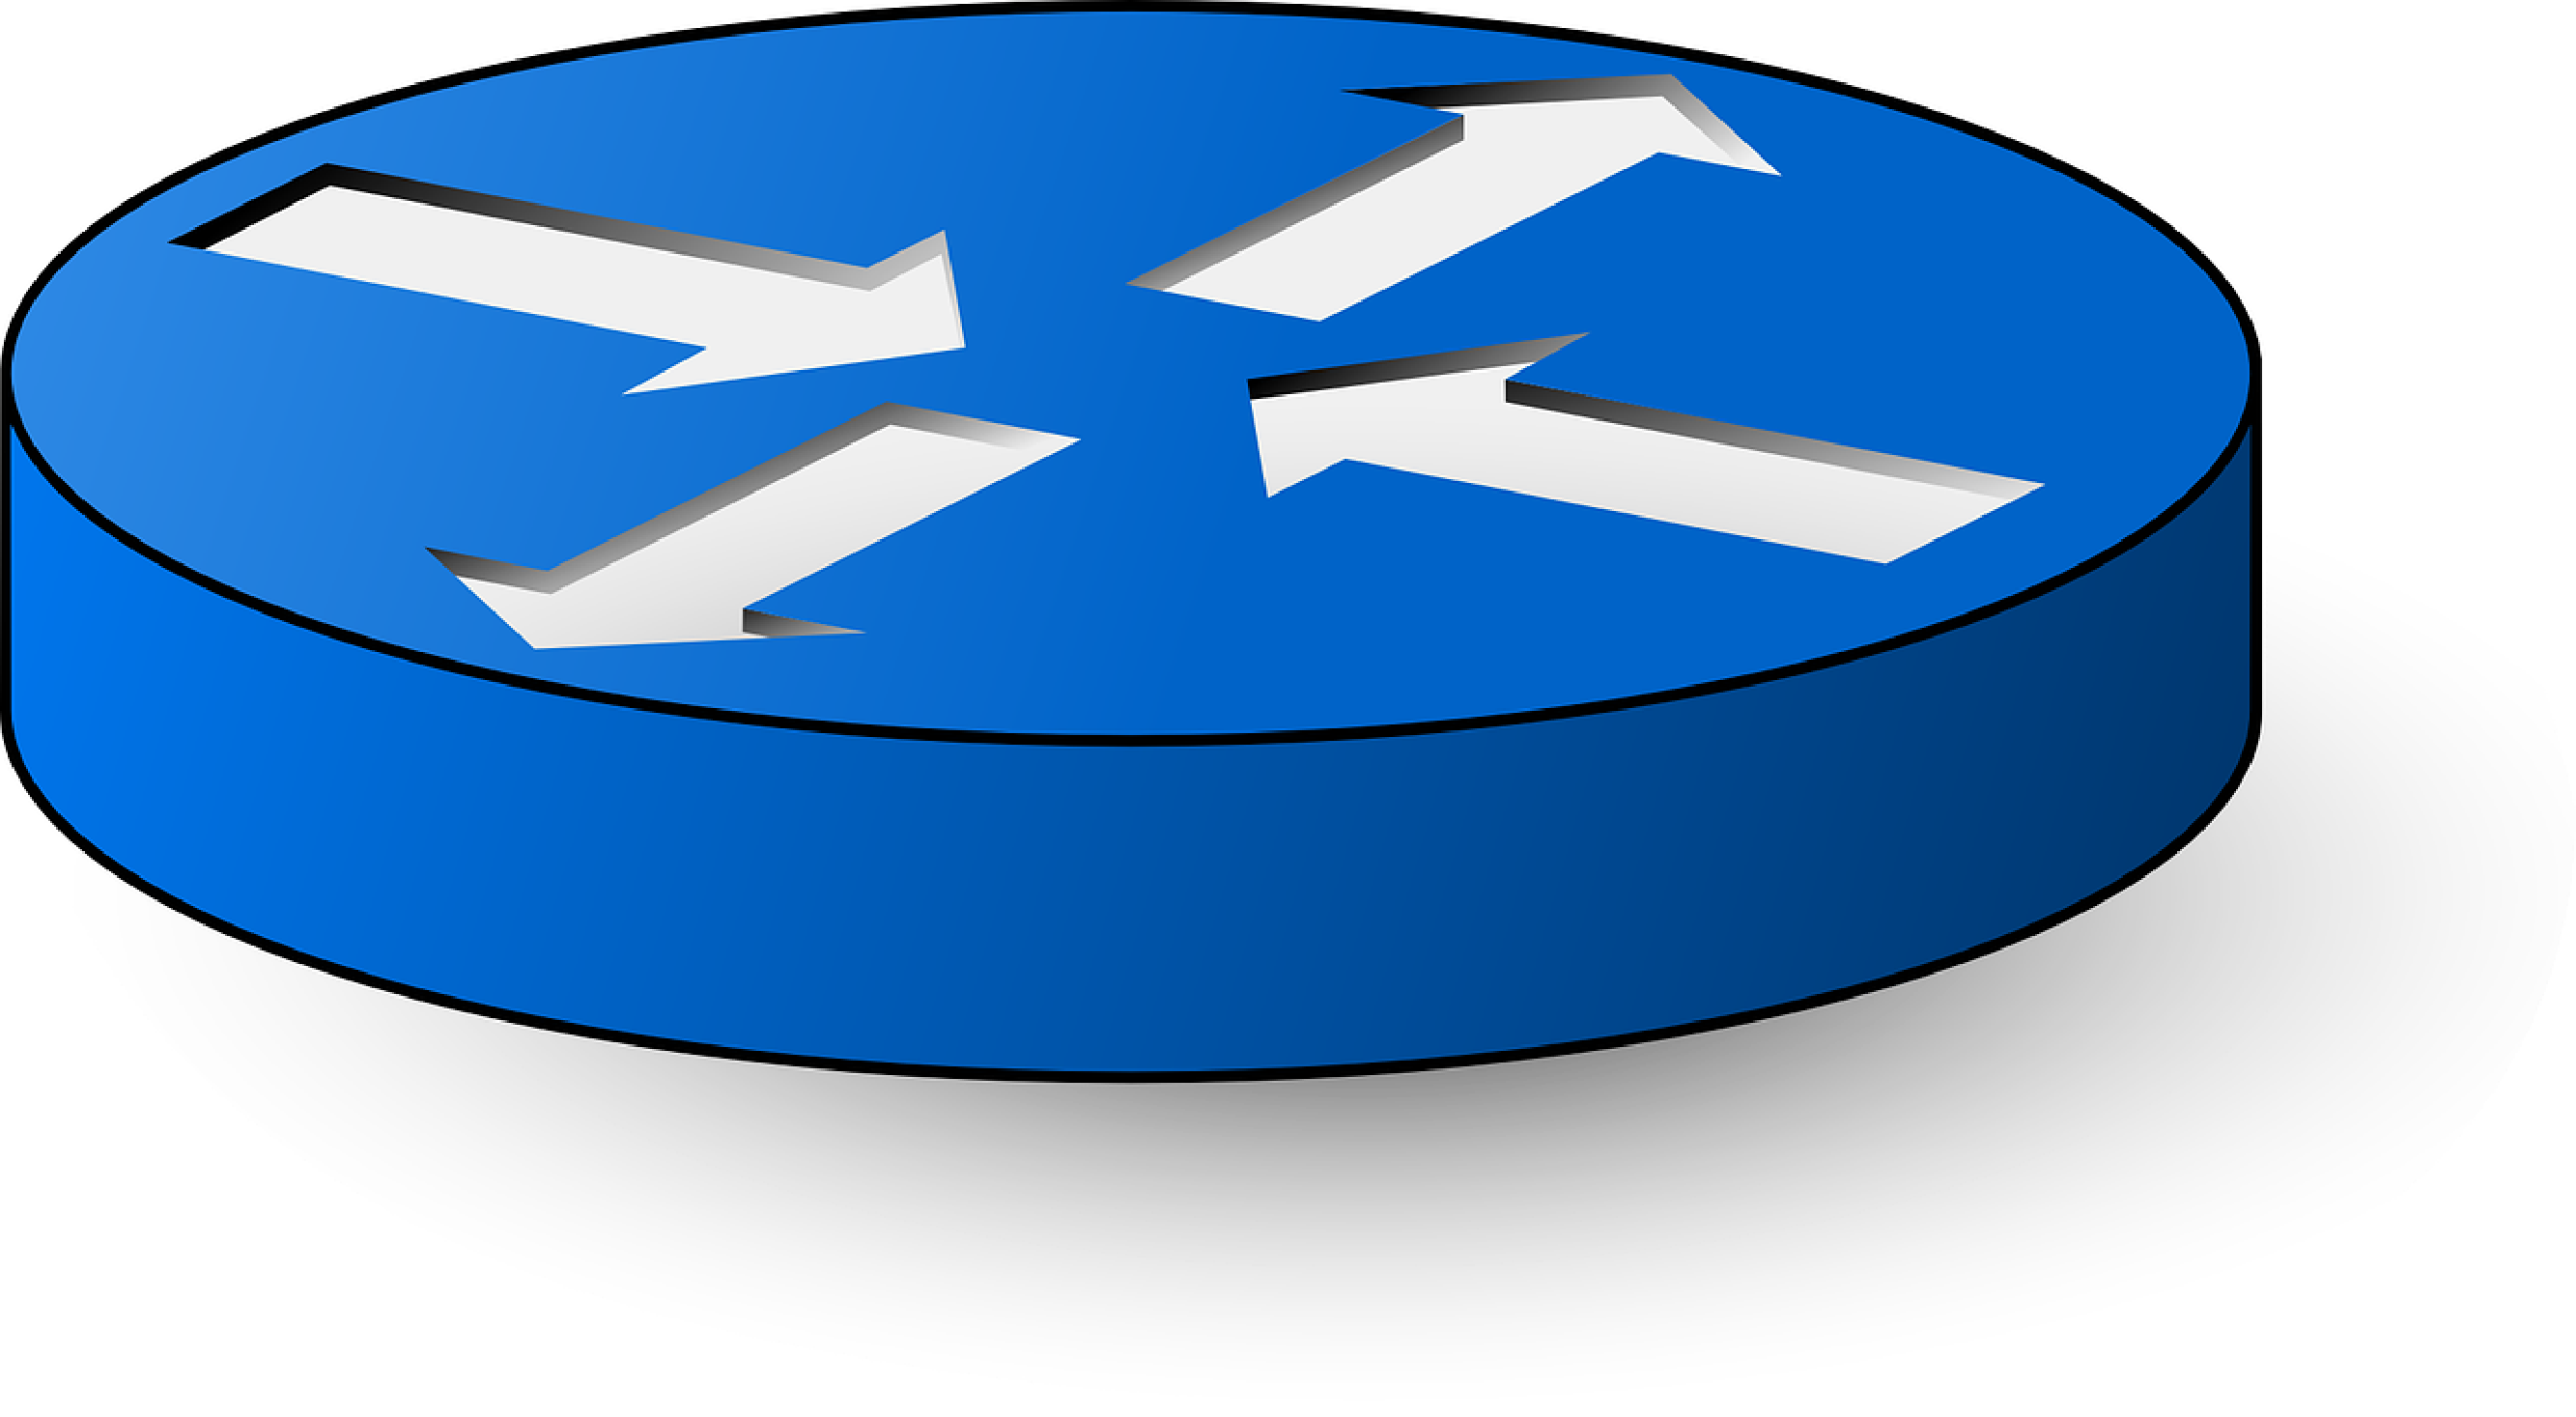
\includegraphics[width=52.5pt,height=52.5pt]{figures/router-30140_1280.pdf}};
%Image [id:dp34021892319279323] 
\draw (515,487.5) node  {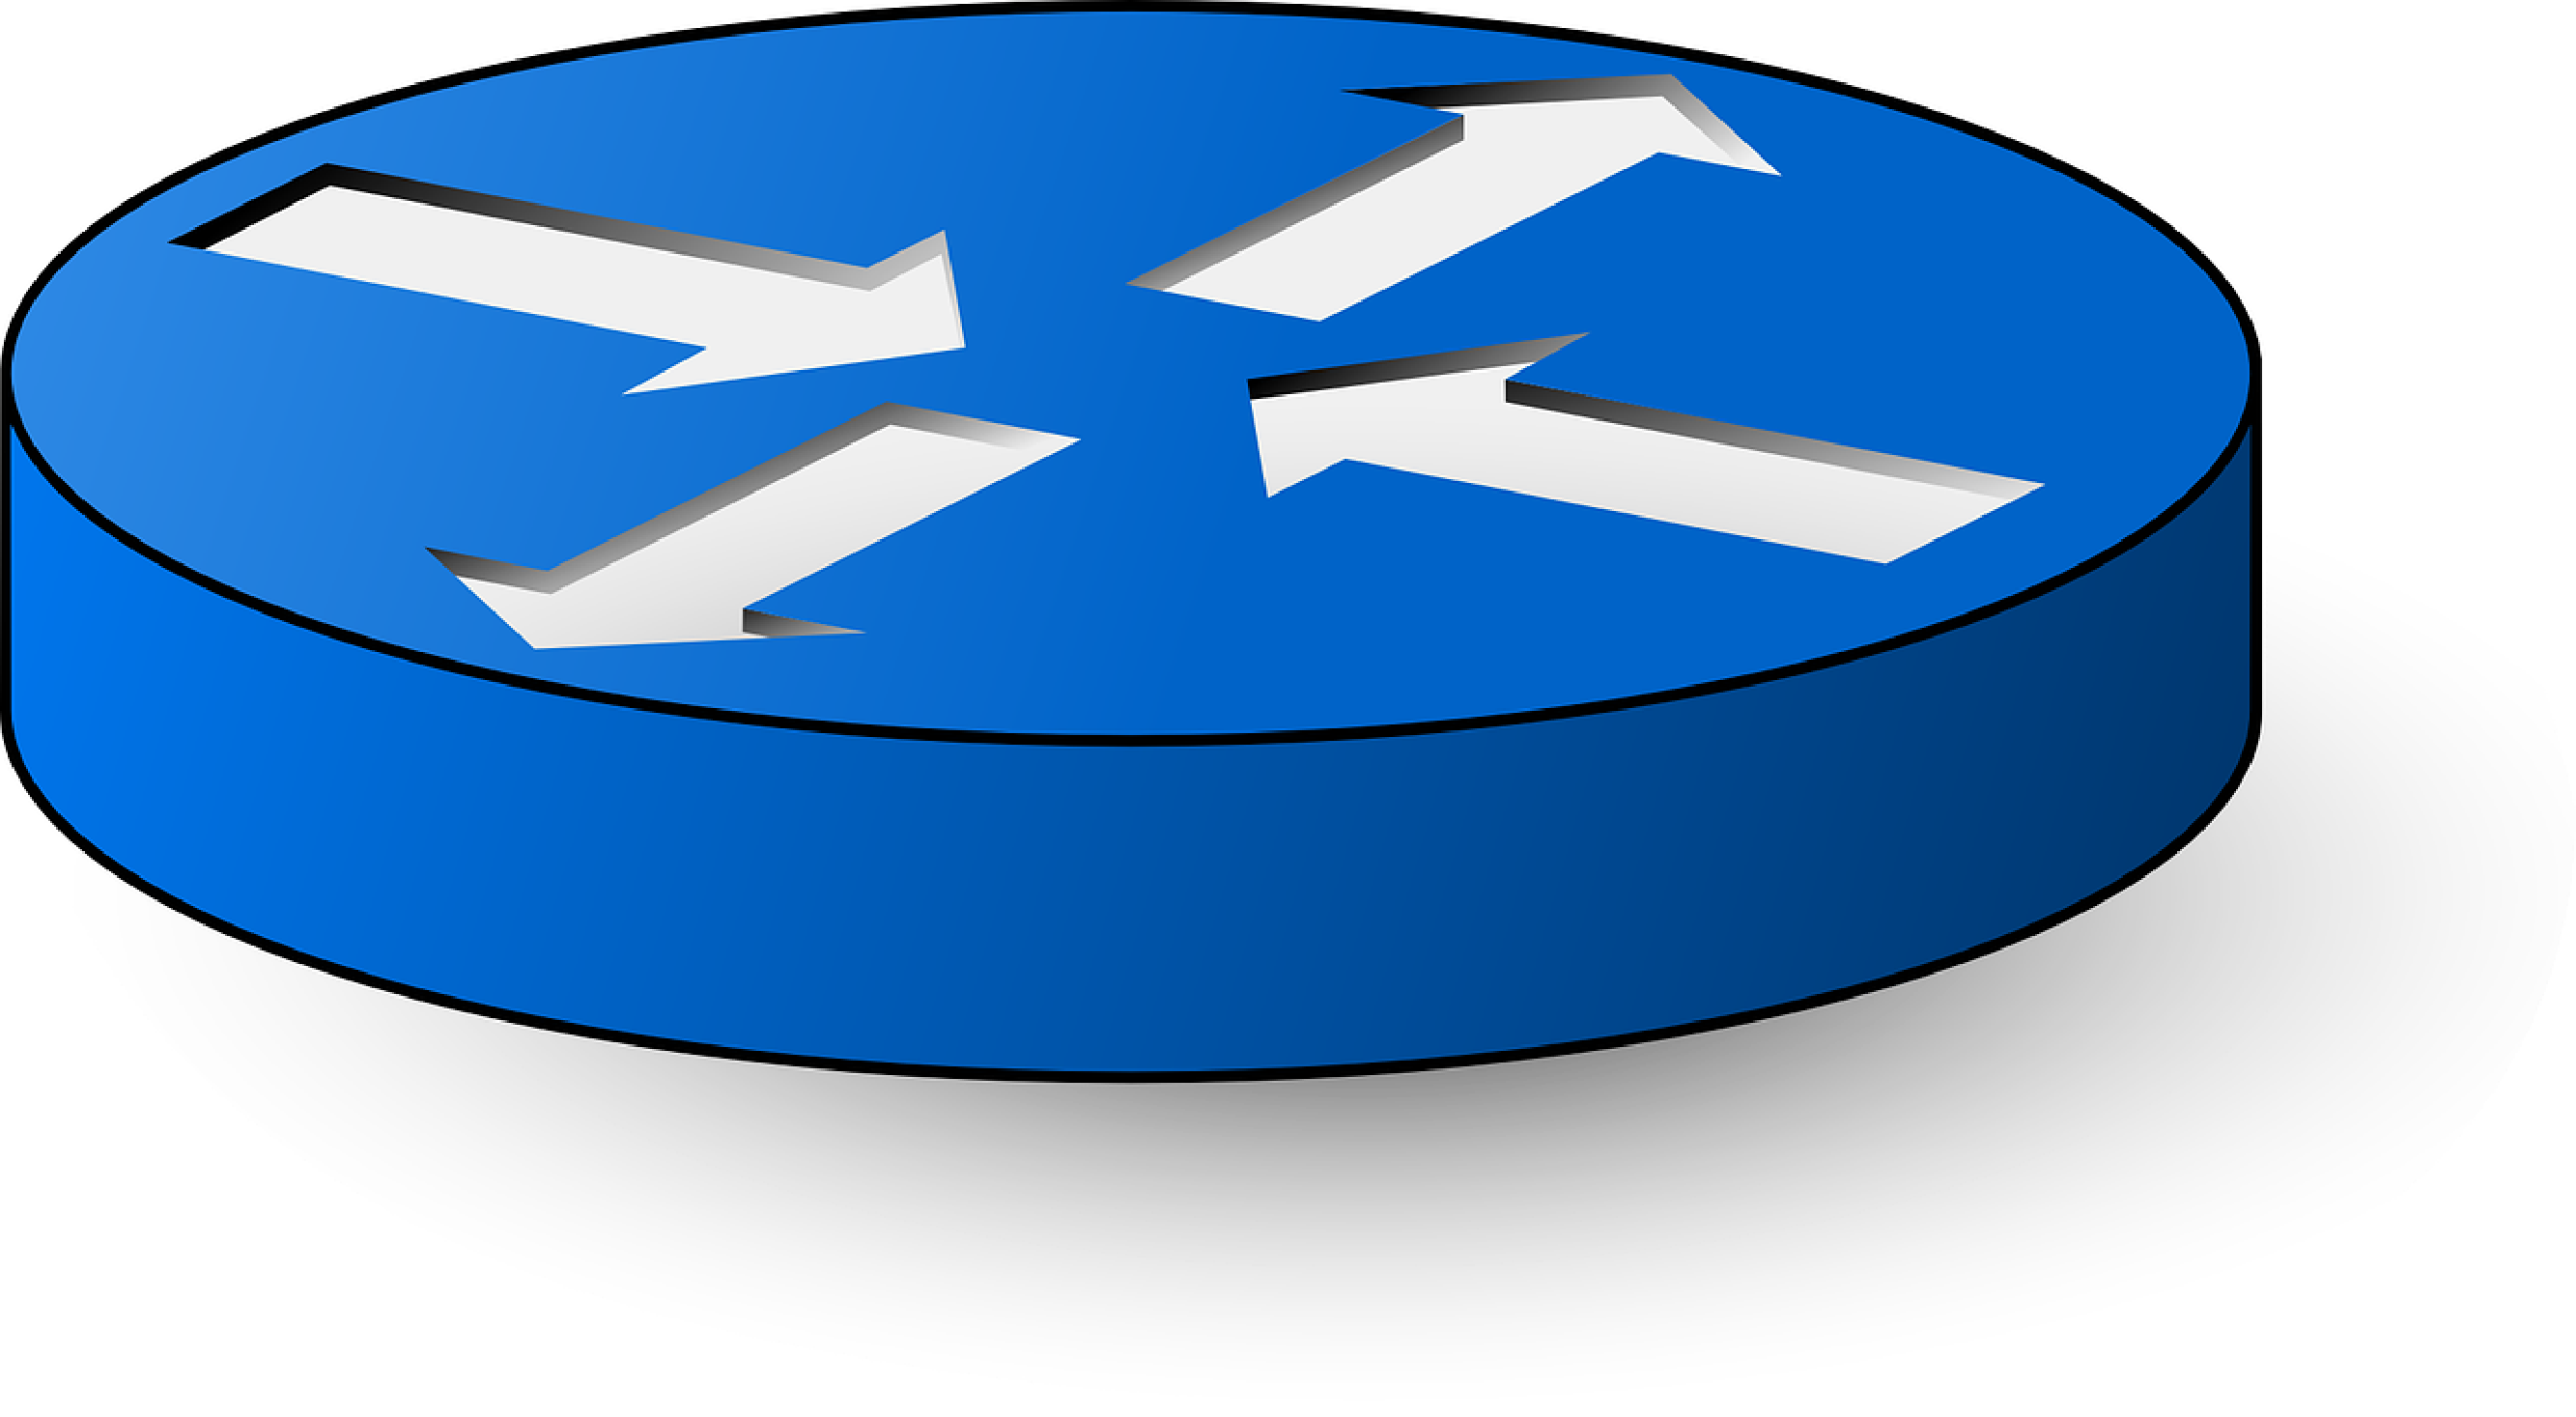
\includegraphics[width=52.5pt,height=52.5pt]{figures/router-30140_1280.pdf}};
%Straight Lines [id:da9221433559107663] 
\draw [line width=1.5]  [dash pattern={on 1.69pt off 2.76pt}]  (63.05,209) -- (62,408.97) ;


%Straight Lines [id:da18979728678812846] 
\draw [line width=1.5]  [dash pattern={on 1.69pt off 2.76pt}]  (139.05,261) -- (140,442.97) ;


%Straight Lines [id:da3949095016333407] 
\draw [line width=1.5]  [dash pattern={on 1.69pt off 2.76pt}]  (178.05,153) -- (186.2,381.27) ;


%Straight Lines [id:da9197957685386293] 
\draw [line width=1.5]  [dash pattern={on 1.69pt off 2.76pt}]  (314.05,169.17) -- (84,411) ;


%Straight Lines [id:da5299009760945013] 
\draw [line width=1.5]  [dash pattern={on 1.69pt off 2.76pt}]  (492.05,168) -- (495.6,384.07) ;


%Straight Lines [id:da535589916512549] 
\draw [line width=1.5]  [dash pattern={on 1.69pt off 2.76pt}]  (390.05,170) -- (390.4,391.27) ;


%Rounded Rect [id:dp33971726070681063] 
\draw  [fill={rgb, 255:red, 217; green, 154; blue, 232 }  ,fill opacity=1 ] (49,306.78) .. controls (49,301.88) and (52.98,297.9) .. (57.89,297.9) -- (543.11,297.9) .. controls (548.02,297.9) and (552,301.88) .. (552,306.78) -- (552,333.45) .. controls (552,338.35) and (548.02,342.33) .. (543.11,342.33) -- (57.89,342.33) .. controls (52.98,342.33) and (49,338.35) .. (49,333.45) -- cycle ;

%Straight Lines [id:da3032548642460361] 
\draw [color={rgb, 255:red, 74; green, 144; blue, 226 }  ,draw opacity=1 ][line width=1.5]    (222.05,340.17) -- (208.13,376.37) ;
\draw [shift={(207.05,379.17)}, rotate = 291.04] [color={rgb, 255:red, 74; green, 144; blue, 226 }  ,draw opacity=1 ][line width=1.5]    (14.21,-4.28) .. controls (9.04,-1.82) and (4.3,-0.39) .. (0,0) .. controls (4.3,0.39) and (9.04,1.82) .. (14.21,4.28)   ;

%Straight Lines [id:da5649833646600878] 
\draw [color={rgb, 255:red, 74; green, 144; blue, 226 }  ,draw opacity=1 ][line width=1.5]    (330.05,344.17) -- (369.08,388.91) ;
\draw [shift={(371.05,391.17)}, rotate = 228.9] [color={rgb, 255:red, 74; green, 144; blue, 226 }  ,draw opacity=1 ][line width=1.5]    (14.21,-4.28) .. controls (9.04,-1.82) and (4.3,-0.39) .. (0,0) .. controls (4.3,0.39) and (9.04,1.82) .. (14.21,4.28)   ;

%Straight Lines [id:da5842761266197537] 
\draw [color={rgb, 255:red, 74; green, 144; blue, 226 }  ,draw opacity=1 ][line width=1.5]    (479.05,343.17) -- (485.53,380.21) ;
\draw [shift={(486.05,383.17)}, rotate = 260.07] [color={rgb, 255:red, 74; green, 144; blue, 226 }  ,draw opacity=1 ][line width=1.5]    (14.21,-4.28) .. controls (9.04,-1.82) and (4.3,-0.39) .. (0,0) .. controls (4.3,0.39) and (9.04,1.82) .. (14.21,4.28)   ;

%Straight Lines [id:da44476437360701715] 
\draw [color={rgb, 255:red, 74; green, 144; blue, 226 }  ,draw opacity=1 ][line width=1.5]    (93.05,345.17) -- (75.9,403.29) ;
\draw [shift={(75.05,406.17)}, rotate = 286.44] [color={rgb, 255:red, 74; green, 144; blue, 226 }  ,draw opacity=1 ][line width=1.5]    (14.21,-4.28) .. controls (9.04,-1.82) and (4.3,-0.39) .. (0,0) .. controls (4.3,0.39) and (9.04,1.82) .. (14.21,4.28)   ;

%Straight Lines [id:da5384124591664345] 
\draw [line width=1.5]  [dash pattern={on 1.69pt off 2.76pt}]  (445.5,16.33) -- (484.5,16.83) ;


%Straight Lines [id:da3606010400838229] 
\draw    (445,32.71) -- (485,33.21) ;


%Straight Lines [id:da015844815365207543] 
\draw [color={rgb, 255:red, 74; green, 144; blue, 226 }  ,draw opacity=1 ][line width=1.5]    (448.5,65.13) -- (478.5,64.97) ;
\draw [shift={(481.5,64.96)}, rotate = 539.71] [color={rgb, 255:red, 74; green, 144; blue, 226 }  ,draw opacity=1 ][line width=1.5]    (14.21,-4.28) .. controls (9.04,-1.82) and (4.3,-0.39) .. (0,0) .. controls (4.3,0.39) and (9.04,1.82) .. (14.21,4.28)   ;

%Straight Lines [id:da6059698523065559] 
\draw [color={rgb, 255:red, 74; green, 144; blue, 226 }  ,draw opacity=1 ][line width=1.5]    (161,343) -- (155.18,439.01) ;
\draw [shift={(155,442)}, rotate = 273.47] [color={rgb, 255:red, 74; green, 144; blue, 226 }  ,draw opacity=1 ][line width=1.5]    (14.21,-4.28) .. controls (9.04,-1.82) and (4.3,-0.39) .. (0,0) .. controls (4.3,0.39) and (9.04,1.82) .. (14.21,4.28)   ;

%Straight Lines [id:da7790467806562547] 
\draw [color={rgb, 255:red, 74; green, 144; blue, 226 }  ,draw opacity=1 ][line width=1.5]    (433,343) -- (487.71,458.29) ;
\draw [shift={(489,461)}, rotate = 244.61] [color={rgb, 255:red, 74; green, 144; blue, 226 }  ,draw opacity=1 ][line width=1.5]    (14.21,-4.28) .. controls (9.04,-1.82) and (4.3,-0.39) .. (0,0) .. controls (4.3,0.39) and (9.04,1.82) .. (14.21,4.28)   ;


% Text Node
\draw (85,498.5) node [scale=0.9] [align=left] {Physical Infrastructure};
% Text Node
\draw (59,137) node  [align=left] {V1};
% Text Node
\draw (119,117) node  [align=left] {V3};
% Text Node
\draw (144,188) node  [align=left] {V2};
% Text Node
\draw (353,111) node  [align=left] {V4};
% Text Node
\draw (437,113) node  [align=left] {V5};
% Text Node
\draw (512,108) node  [align=left] {V6};
% Text Node
\draw (54,475) node  [align=left] {P1};
% Text Node
\draw (205,486) node  [align=left] {P2};
% Text Node
\draw (244,390) node  [align=left] {P3};
% Text Node
\draw (342,397) node  [align=left] {P4};
% Text Node
\draw (561,394) node  [align=left] {P5};
% Text Node
\draw (565,473) node  [align=left] {P6};
% Text Node
\draw (531,16) node  [align=left] {Virtual Link};
% Text Node
\draw (538,37) node  [align=left] {Physical Link};
% Text Node
\draw (572,59) node  [align=left] {Hypervisor - Switch link};
% Text Node
\draw (300.5,320.11) node  [align=left] {Network Hypervisor : hname1};
% Text Node
\draw (69,104.5) node  [align=left] {{\small vSDN1}};
% Text Node
\draw (309,97.5) node [scale=0.9] [align=left] {{\small vSDN2}};


\end{tikzpicture}

\caption{Example of infrastructure  modeling}
\label{fig:VNE-example-model}
\end{figure}

The current infrastructure gives the following formal declaration:

\begin{myformula}
/* Defining Virtual Networks */\\
virtual\_network(vSDN1,ti1)\\
virtual\_network(vSDN2,ti1)\\
\textbf{\\}
/* Assigning virtual nodes and links to each VN */\\
virtual\_node(V1,vSDN1,ti1)\\
virtual\_node(V2,vSDN1,ti1)\\
virtual\_node(V3,vSDN1,ti1)\\
virtual\_node(V4,vSDN2,ti1)\\
virtual\_node(V5,vSDN2,ti1)\\
virtual\_node(V6,vSDN2,ti1)\\
virtual\_link(vlink1,V1,V2,vSDN1,ti1)\\
virtual\_link(vlink2,V1,V3,vSDN1,ti1)\\
virtual\_link(vlink3,V4,V5,vSDN2,ti1)\\
virtual\_link(vlink4,V5,V6,vSDN2,ti1)\\
\textbf{\\}
\textbf{\\}
/* Defining physical nodes and links in the infrastructure */\\
physical\_node(P1,ti1)\\
physical\_node(P2,ti1)\\
physical\_node(P3,ti1)\\
physical\_node(P4,ti1)\\
physical\_node(P5,ti1)\\
physical\_node(P6,ti1)\\
physical\_link(plink1,P1,P2,ti1)\\
physical\_link(plink2,P1,P3,ti1)\\
physical\_link(plink3,P2,P4,ti1)\\
physical\_link(plink4,P3,P4,ti1)\\
physical\_link(plink5,P4,P5,ti1)\\
physical\_link(plink6,P4,P6,ti1)\\
\textbf{\\}
/* Defining the hypervisor*/\\
hypervisor(h1,ti1)\\
\textbf{\\}
/* Defining the physical path connecting the physical nodes to the hypervisor */\\
physical\_path(ppath1,P1,h1,ti1)\\
physical\_path(ppath2,P2,h1,ti1)\\
physical\_path(ppath3,P3,h1,ti1)\\
physical\_path(ppath4,P4,h1,ti1)\\
physical\_path(ppath5,P5,h1,ti1)\\
physical\_path(ppath6,P6,h1,ti1)\\
\textbf{\\}
/* Assigning the hypervisor to each physical node */\\
hypervisor\_of(h1,P1,ppath1,ti1)\\
hypervisor\_of(h1,P2,ppath2,ti1)\\
hypervisor\_of(h1,P3,ppath3,ti1)\\
hypervisor\_of(h1,P4,ppath4,ti1)\\
hypervisor\_of(h1,P5,ppath5,ti1)\\
hypervisor\_of(h1,P6,ppath6,ti1)\\
\textbf{\\}
/* Defining the embedding of virtual elements in physical ones */\\
node\_embedding(V1,P1,ti1)\\
node\_embedding(V4,P1,ti1)\\
node\_embedding(V2,P2,ti1)\\
node\_embedding(V3,P3,ti1)\\
node\_embedding(V5,P4,ti1)\\
node\_embedding(V6,P5,ti1)\\
link\_embedding(vlink1,plink1,ti1)\\
link\_embedding(vlink2,plink2,ti1)\\
link\_embedding(vlink3,plink2,ti1)\\
link\_embedding(vlink3,plink4,ti1)\\
link\_embedding(vlink4,plink5,ti1)
\end{myformula}
% \GB{I do not get why vlink3 is not mapped to a path instead. Or you should get rid of this path concept and only keep list of links.}
% \FC{Paths are only physical, as they represent the path between a node and the hypervisor. Without this notion you have to rethink the whole path properties defined later on, because the attacker has to be on the path of the communication to be able to intercept/attack it.}\GB{OK. So please explain it this way so that it is more explicit to the reader.}

\subsection{Modeling the migration of Virtual Networks}
\label{sec:migration}
In a SDN virtualization infrastructure, the virtual networks are operated by installing flow rules in the underlying physical network.
In the event of a migration, for maintenance purposes or because of an attack, the flow rules will be redeployed on a different physical substrate.
Determining how the flow rules should be deployed and which physical nodes should be selected is called Virtual Network Embedding, and there already are various solutions doing so~\cite{Zangiabady2017e, Papagianni2013, Chowdhury2016d, Wang2015}.
We leave the VNE problem out of the scope of this thesis.
We also limit our study of migration process to the networking aspect of it, meaning that we are not considering the internal specificities of the hypervisors and how mappings between virtual and physical nodes are handled during the migration.
We study the flow rules that will be installed in the SDN nodes by the hypervisor because of the migration, and how the migration can be exploited for unlawful purposes.

\begin{figure}[ht]
\centering
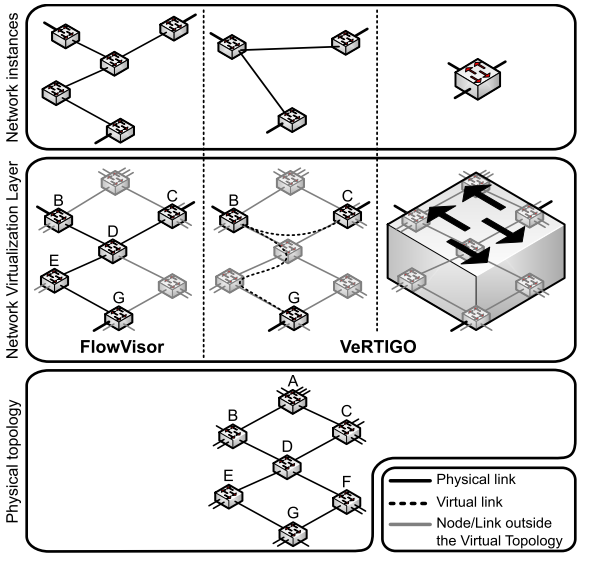
\includegraphics[scale=0.8]{figures/onetomany.png}
\caption{Example of 1-to-many mapping for virtual nodes and links, from VeRTIGO~\cite{VeRTIGO-Corin2012a}}
\label{fig:1tomany}
\end{figure}
\subsubsection{Modeling the migration process}
We have presented in Section~\ref{sec:reference_archi} a reference architecture for the network hypervisor.
From the SDN point of view, a virtual link is a collection of flow rules deployed on one ore more physical nodes, to carry the traffic of a specific tenant.
Similarly, a virtual node is the end point of several flow rules.
Therefore, a virtual node can be seen a collection of flow rules describing the end point of several virtual links, SDN-wise.

We include in this work the possibility to describe a one-to-many mapping between a virtual node and a physical node.
Figure~\ref{fig:1tomany} (from VeRTIGO~\cite{VeRTIGO-Corin2012a}) depicts the one to many mapping between virtual and physical elements. The virtual network is composed of three nodes embedded by physical nodes B, C and G.
The virtual link connecting virtual nodes between B and G is seen as a single link while actually there are physical nodes D and E and the corresponding physical links supporting the embedding.
Thus, one virtual link is mapped to many physical resources.

We describe two migration algorithms in the following subsections, a naive algorithm and a more elaborate one. 
The ordering of the selection of nodes and links for the migration is studied in~\cite{vnm-lo2013}. 
We consider this to be out of scope of this thesis and we chose a naive ordering for the implementation of the migration algorithms.
We propose our version of this algorithm (see Algorithm~\ref{algo:move_algo}) where during the migration phase, both VNs (old and new) will coexist to maintain the availability of the virtual network.


These algorithms use different functions in order to migrate the topology: create\_link, delete\_link, create\_node, delete\_node and embedding. 
Each function will be associated to predicates representing the state of the virtual networks during the migration.
We explain what each function does, SDN-wise:

\begin{itemize}
\item Create\_link($vlink\_name,embed$): This function will deploy flow rules related to $vlink\_name$ on the different nodes composing $embed$. It generates $virtual\_link$ and $link\_embedding$ predicates, and returns the identifier of the migrated link.
\item Delete\_link($vlink\_name$): This function will remove the flow rules pertaining to $vlink\_name$ from the physical nodes embedding it.
\item Create\_node($vnode\_name,embed$): This function will deploy flow rules related to $vnode\_name$ on the different nodes composing $embed$. It generates $virtual\_node$ and $node\_embedding$ predicates, and returns the identifier of the migrated node.
\item Delete\_node($vnode\_name$): This function will remove the flow rules related to  $vnode\_name$ on the physical nodes embedding it.
\item embedding($vlink\_name|vnode\_name$) returns the set of resources used for the embedding of either $vlink\_name$ or $vnode\_name$. It is then used to instantiate virtual nodes and links.
\end{itemize}



\subsubsection{Move based migration algorithm}
\label{sec:move-algo}

An intuitive migration algorithm is described in~\cite{Lime-Ghorbani2014}. 
This algorithm aims at migrating the resources all at once.
However, during the migration phase, the VNs are not operational as both are shutdown.
We propose our version of this algorithm (see Algorithm~\ref{algo:move_algo}) where during the migration phase, both VNs (old and new) will coexist to maintain the availability of the virtual network.

First (line 3) we initialize $new\_topology$ as the migrated topology. Then, for each virtual node in the topology, we retrieve the new embedding decided by the VNE component (lines 4-5).
Then (line 6) we instantiate the new virtual node and add the information to $new\_topology$
We repeat the process for the virtual links (lines 7-9).
Then we remove the flow rules related to the old virtual nodes from the original substrate (lines 10-11) and from the old virtual links (lines 12-13).

An underlying aspect of the coexistence of the old and new VNs is the necessity to redirect new incoming flows through the newly migrated VN instead of the old one.
This is handled by setting specific priorities for the flow rules corresponding to the VN.


\begin{algorithm}[ht]
\textbf{Input: }$topology$ as the virtual network\\
\textbf{Output: } $new\_topology$ as the migrated topology\\
% \State $nodes \gets List\_of\_nodes(topology)$
$new\_topology \gets \{\emptyset\}$\\
\For{$node$ \textbf{in} $topology$}{
$embed \gets$ embedding($node$)\\
$new\_topology \gets$~$new\_topology$~$\cup$~create\_node($node$,$embed$)
}
\For{$link$ \textbf{in} $topology$}{
$embed \gets$ embedding($link$)\\
$new\_topology \gets$~$new\_topology$~$\cup$~create\_link($link$,$embed$)
}
\For{$node$ \textbf{in} $topology$}{
delete\_node($node$)
}
\For{$link$ \textbf{in} $topology$}{
delete\_link($link$)
}
\caption{Move based algorithm}
\label{algo:move_algo}
\end{algorithm}


\subsubsection{Iterative migration algorithm}
Another algorithm we consider is described in~\cite{vnm-lo2013}.
This algorithm iteratively moves nodes one after another, while dynamically creating links for the migrated nodes and deleting the old ones.
We represent this algorithm in pseudo-code in Algorithm~\ref{algo:iterative_algo}.
% Create two arrays, one to hold nodes left to be migrated, one to hold the nodes that have been migrated (lines 2-3).

First, initialize a counter to remember the number of iterations of the algorithm (Line 5).
% While there are nodes to be migrated, do the following (Lines 5 to 28):
Select a node among the remaining nodes (line 7), we refer to it as node $n$. Instantiate the new node (line 9) and create the virtual links between the new node and the nodes that have not been migrated (lines 11-14).
If this is not the first iteration of the algorithm, there might be virtual links that must be deployed between the new node and the nodes that have already been migrated. (lines 15-20).
There may also be links between migrated nodes and the old node.
If so, they are deleted. (lines 21-24)



\textbf{Input: }$topology$ as the virtual network\\
\begin{algorithm}[ht]
\textbf{Output: } $new\_topology$ as the migrated topology\\
 $remaining\_nodes \gets list\_of\_nodes(topology)$\\
 $migrated\_nodes \gets \emptyset$\\
 $iter \gets 1$\\
\While {$remaining\_nodes \neq \emptyset$}{
 $n \gets Select\_node(remaining\_nodes)$\\
 $embed \gets$ embedding($n$)\\
 $new\_n \gets$ create\_node($n,embed$)\\
 \For{$node$ \textbf{in} $remaining\_nodes$}{
    \uIf{exist\_link($new\_n,node,topology$)}{
        $vlink \gets $link($new\_n,node,topology$)\\
        $embed \gets$ embedding($vlink,topology$)\\
        create\_link($vlink,embed$)\\
    }
 }
%  $Deploy\_links(new\_n,remaining\_nodes,topology)$\\
\uIf{$iter>1$}{
%  $Deploy\_links(new\_n,migrated\_nodes,topology)$\\
 \For{$node$ \textbf{in} $migrated\_nodes$}{
    \uIf{exist\_link($new\_n,node,topology$)}{
        $vlink \gets $link($new\_n,node,topology$)\\
        $embed \gets$ embedding($vlink,topology$)\\
        create\_link($vlink,embed$)\\
    }
 }
%  $Deleted\_links(n,migrated\_nodes,topology)$
 \For{$node$ \textbf{in} $migrated\_nodes$}{
    \uIf{exist\_link($new\_n,node,topology$)}{
        $vlink \gets $link($new\_n,node,topology$)\\
        delete\_link($vlink$)
    }
 }
 
 }
 $iter \gets iter + 1$\\
 $migrated\_nodes \gets migrated\_nodes \cup n$\\
 $remaining\_nodes \gets remaining\_nodes / \{n\}$\\
 $delete\_node(n)$\\
 }
\caption{Iterative migration algorithm}
\label{algo:iterative_algo}
\end{algorithm}


The following list details the functions used for the migration
%\GB{again, you are not providing an elaborate explanation with respect to the parameters.}.
%\FC{Done}
\begin{itemize}
\item Select\_node selects the next node to be migrated.
\item exist\_link($node1,node2,topology$) returns True if there is a virtual link between $node1$ and $node2$ in $topology$.
\item link($node1,node2,topology$) returns the identifier of the virtual link connecting $node1$ and $node2$ in $topology$.
\end{itemize}

\subsection{Security properties applied to Virtual Network migration}
\label{sec:security_prop}
In this section, we define the different security properties we consider in the environment during the migration.
We propose several security properties: confidentiality, integrity, availability, usually referred to as CIA~\cite{ISO/IEC270012013}, and we introduce co-residency.
After providing a formal definition of the security property, we refine it into several properties related to the operation of SDN networks and virtualization. Each property concerns physical elements of the SDN infrastructure, and we provide the equivalent properties for the virtual nodes and links if they exist. 
% For the rest of this section, we note $E_n$ (respectively $E_l$) the underlying resources embedding virtual node $n$ (respectively virtual link $l$).

\subsubsection{Confidentiality}
\label{sec:prop-conf}
Confidentiality is a characteristic that applies to information.
To protect and preserve the confidentiality of information means to ensure that it is not made available or disclosed to unauthorized entities~\cite{ISO/IEC270012013}.
Therefore, in network security, the confidentiality of a message in transit in the network is defined by the ability of an authorized  user to read data forwarded by an element of the network.
Formally we can define a predicate $confidentiality(D)$ as follows:

\begin{myformula}
$ confidentiality(D) \Leftrightarrow \forall U,t~reads(U,D,t) \Rightarrow is\_data\_authorized(U,D,t)$
\end{myformula}

\begin{itemize}
\item $reads(U,D,t)$ is true if user $U$ reads data $D$ at time $t$.
\item $is\_data\_authorized(U,D,t)$ is true if user $U$ has the right to read data $D$ at time $t$.
%\item $\overline{reads(U,D,t)}$ is the negation of $reads(U,D,t)$
\end{itemize}
Simply put, if at any time no user reads $D$ or every user reading $D$ is authorized to do so, then the confidentiality of $D$ is preserved.
From a cryptographical perspective, ciphered data and plain text data are treated as the same regarding their confidentiality while in transit in the network.
Obviously, ciphered data is more secured than plain text data but this is not in the scope of this model.\\
From this definition, we can describe several properties directly affecting the physical and virtual topology.


% Give names instead of numbers 1, 2?
% node versus network element.  are they the same?

\textbf{Property 1a:} A physical node respects the confidentiality of the data it is carrying if and only if the user accessing the node and the data is authorized to do so.
%\RW{is the table helpful?  the formula seems clearer to me. rw}\FC{Cleaned}
\newline \textbf{Formal definition:} Let $N$ be a network element, $U$ a user (malicious or not), $D$ the data carried by the network, and $t$ the time.


\begin{myformula}
$node\_confidentiality(N) \Leftrightarrow \forall D,U,t~
confidentiality(D) \wedge is\_carrying(N,D,t) \wedge (accessing(U,N,t) \Rightarrow is\_node\_authorized(U,N,t))$
\end{myformula}

\begin{itemize}
\item $accessing(U,N,t)$ is true if user $U$ accesses network element $N$ at time $t$.
\item $is\_node\_authorized(U,N,t)$ is true if the user $U$ has the right to access network element $N$ at time $t$.
\item $is\_carrying(N,D,t)$ is true if node $N$ is carrying data $D$ at time $t$.
\end{itemize}

\textbf{Property 1b:} A virtual node respects the confidentiality of the data it is carrying if and only if the embedding nodes respect the confidentiality of the data as well.
%\RW{is the table helpful?  the formula seems clearer to me. rw}\FC{Cleaned}
\newline \textbf{Formal definition:} Let $n$ be a virtual node and $E_n$ the physical resources embedding $n$.


\begin{myformula}
$vnode\_confidentiality(n) \Leftrightarrow \bigwedge\limits_{N\in E_n} node\_confidentiality(N) $
\end{myformula}

\textbf{Property 1c:} A virtual link respects the confidentiality of the data it is carrying if and only if the embedding nodes respect the confidentiality of the data as well.
%\RW{is the table helpful?  the formula seems clearer to me. rw}\FC{Cleaned}
\newline \textbf{Formal definition:} Let $l$ be a virtual link and $E_n$ the physical resources embedding $n$.


\begin{myformula}
$vlink\_confidentiality(l) \Leftrightarrow \bigwedge\limits_{N\in E_n} node\_confidentiality(N) $
\end{myformula}

\textbf{Property 2:} A path preserves confidentiality from end to end if all of its network elements preserve their own confidentiality.
\newline \textbf{Formal definition:} Let $P$ be the path taken by the traffic, $L_N^P$ be the list of nodes composing $P$.

\begin{myformula}
$path\_confidentiality(P) \Leftrightarrow \bigwedge\limits_{n \in L_N^P}node\_confidentiality(n)$
\end{myformula}

% \textbf{Property 2b:} A virtual path preserves confidentiality from end to end if all of its virtual nodes and links preserve their own confidentiality.
% \newline \textbf{Formal definition:} Let $P$ be the path taken by the traffic, $L_N$ be the list of virtual nodes composing $P$, and $L_L$ the list of virtual links composing $P$.
% % and $L_{s}$ be the list of the links between each node of $P$.
% \begin{myformula}
% $vpath\_confidentiality(P) \Leftrightarrow \bigwedge\limits_{n \in L_N}vnode\_confidentiality(n) \wedge \bigwedge\limits_{l \in L_L}vlink\_confidentiality(l)$
% \end{myformula}

\textbf{Property 3:} A node's configuration remains confidential during a migration if the employed communication channel respects the confidentiality of the communication.
\newline \textbf{Formal definition:} Let $N$ be a node, $conf$ be the configuration to be pushed, $C$ be an hypervisor.
\newline

\begin{myformula}
$config\_confidentiality(conf,N) \Leftrightarrow~\exists~C,P, 
is\_hypervisor\_of(C,N) \wedge is\_path(C,P,N) \wedge  conf\_of\_node(conf,N) \Rightarrow
~path\_confidentiality(P) \wedge  node\_confidentiality(N)
$
\end{myformula}


\begin{itemize}
\item $is\_hypervisor\_of(C,N)$ is true if the hypervisor $C$ is affected to node $N$.  
\item $is\_path(C,P,N)$ is true if path $P$ is the path between $C$ and $N$.
\item $conf\_of\_node(conf, N)$ is true if node $N$ is running configuration $conf$.
\end{itemize}

\subsubsection{Integrity}
\label{sec:prop-int}
 Preserving the integrity of information means protecting the accuracy and completeness of the information and the methods that are used to process and manage it~\cite{ISO/IEC270012013}.
We emphasize on the fact that the integrity property is evaluated over a period of time instead of being instantaneous.
%\RW{unclear--why "therefore";  what are the temporal values of a piece of information? is that the result of eval at a given time?}\FC{Yes, the integrity of information means that it remains constant through time, unless processed, obviously}

We define two predicates, $d\_integrity(D,ti)$ and $p\_integrity(P,D,N,ti)$, which represent  the integrity of the data $D$ itself and the integrity of the process $P$ used by node $N$ to manipulate $D$, over a time interval $ti$. 

Therefore, if a data has not been legitimately processed, its integrity holds if it hasn't been modified in any other way.
\begin{myformula}
$d\_integrity(D,ti) \Leftrightarrow \forall t_1,t_2\in ti ~ \overline{processed(D, ti)} \Rightarrow 
~D_{t_1}=D_{t_2}$ 
\end{myformula}
%\RW{I changed the formatting for clarity}

\begin{itemize}
\item $processed(D, ti)$ holds true if $D$ has been legitimately processed during time interval $ti$.
% \item $deval(D,t)$ returns the value of $D$ at time $t$
%\RW{Does this mean that it is not defined if D has been legitimately processed?  Or it is true if D has been processed? or it does not hold if D has been processed?}\FC{It is still true if D has been legally processed}

\end{itemize}

\begin{myformula}
$p\_integrity(P, ti) \Leftrightarrow \forall t_1,t_2 \in ti~ \overline{modified(P, ti)}\Rightarrow 
~P_{t_1}=P_{t_2}$
\end{myformula}

\begin{itemize}
\item $modified(P,ti)$ holds true if process $P$ has been modified legitimately during time interval ti
\item $peval(P,t)$ returns the process $P$ at time $t$
\end{itemize}
%\RW{you use P for paths and processes. and p for a function. what is the output of data? is it the value (eval?)}\FC{I don't understand}\GB{beware: you've been using $P$ for two distinct notions. I think that what RW means it that $p$ evaluates the realization of process $P$ over data $D$. In that sense you could, replace $p$ by the keyword $eval$}


\textbf{Property 1a:} The integrity of a network element is preserved if the data it carries and the process used to process it have their integrity preserved. 
\newline
\textbf{Formal definition:} Let $N$ be a network element, $D$ some data and $P$ a function modeling the process used by $N$ to handle data $D$.

\begin{myformula}
$node\_integrity(N) \Leftrightarrow \forall D,ti,\exists P~p\_integrity(P,ti) \wedge d\_integrity(D,ti) \wedge process\_of(N,P,ti)$
\end{myformula}

\begin{itemize}
\item $process\_of(P,N,ti)$ affects process $P$ to node $N$ during time interval ti.
\end{itemize}

\textbf{Property 1b:} The integrity of a virtual node is preserved if and only if the nodes embedding it preserve their integrity as well.
\newline
\textbf{Formal definition:} Let $n$ be a virtual node and $E_n$ the list of nodes embedding $n$.

\begin{myformula}
$vnode\_integrity(n) \Leftrightarrow \bigwedge\limits_{N \in E_n} node\_integrity(N)$
\end{myformula}

\textbf{Property 1c:} The integrity of a virtual link is preserved if and only if the nodes embedding it preserve their integrity as well.
\newline
\textbf{Formal definition:} Let $l$ be a virtual link and $E_l$ the list of nodes embedding $l$.

\begin{myformula}
$vlink\_integrity(n) \Leftrightarrow \bigwedge\limits_{N \in E_l} node\_integrity(N)$
\end{myformula}


\textbf{Property 2:} A path preserves integrity from end to end if all of its network elements preserve their own integrity.
\newline \textbf{Formal definition:} Let $P$ be a path in the network and $L^P_N$ be the list of nodes composing $P$.
\newline

\begin{myformula}
$path\_integrity(P) \Leftrightarrow \bigwedge\limits_{n \in L_N}integrity(n) $
\end{myformula}

% \textbf{Property 2b:} A virtual path preserves integrity from end to end if all its virtual nodes and links preserve their own integrity.
% \newline \textbf{Formal definition:} Let $P$ be a virtual path, $L^P_N$ be the list of virtual nodes composing $P$ and $L_L$ be the list of virtual links composing $P$ .
% \newline

% \begin{myformula}
% $vpath\_integrity(P) \Leftrightarrow \bigwedge\limits_{n \in L^P_N}vnode\_integrity(n) \wedge \bigwedge\limits_{l \in L_L}vlink\_integrity(l) $
% \end{myformula}

\textbf{Property 3:} A node's configuration maintains its integrity during a migration if it is not altered during the installation from the hypervisor to the node.
\newline \textbf{Formal definition:} Let $N$ be a node, $conf$ be the configuration data to be pushed on node $N$, $C$ be a network hypervisor.
\newline
%\RW{ i proposed a replacement but i still have questions about it:  $confidentiality(conf,N) \Leftrightarrow \exists C,P~ confidentiality(C) \wedge confidentiality(P) \wedge confidentiality(N) \wedge is\_controller\_of(C,N)$}
%\RW{needs quantifiers for C U P N.  also, the formula does not constrain these to have anything to do with conf it seems that to define a confidentiality-preserving migration requires mentioning time.  the network is confidential after the migration if it was confidential before.  }

\begin{myformula}
$config\_integrity(conf,N) \Leftrightarrow~\forall ti,\exists~C,P 
~is\_hypervisor\_of(C,N) \wedge is\_path(C,P,N) \wedge  conf\_of\_node(conf,N) \Rightarrow
~d\_integrity(conf,ti)
$
\end{myformula}

\begin{itemize}
\item $is\_hypervisor\_of(C,N)$ is true if the hypervisor $C$ is affected to node $N$.  
\item $is\_path(C,P,N)$ is true if path $P$ is the path between $C$ and $N$..
\item $conf\_of\_node(conf, N)$ is true if node $N$ is running configuration $conf$.
\end{itemize}

\subsubsection{Availability}
\label{sec:prop-avail}
An asset is available if it is accessible and usable when
needed by an authorized entity~\cite{ISO/IEC270012013}.

We can define the predicate $availability(A)$ which represents the availability of asset $A$.
\newline
Let $A$ be an asset, $U$ a user and $ti$ a time interval.
\newline
%\RW{why would availability be discussed without specifying a time?  it seems unlikely that an asset is always useable.}
%\FC{In the same way we consider confidentiality and integrity, as long availability is preserved we don't need time, but we need to pinpoint the time intervals related to the violation if needed.}

\begin{myformula}
$availability(A) \Leftrightarrow \forall ti~is\_accessible(U,A,ti) \wedge is\_usable(U,A,ti) \Rightarrow is\_asset\_authorized(U,A,ti)$
\end{myformula}

% \RW{why would an asset not be available, if it is useable and the user is authorized?  is it because an authorized path does not exist?}
% \FC{I've added authorization}
\begin{itemize}
\item $is\_accessible(U,A,ti)$ is true if user $U$ can contact asset $A$ during time interval $ti$.
\item $is\_usable(U,A,ti)$ is true if user $U$ can use asset $A$ during time interval $ti$.
\item $is\_asset\_authorized(U,A,ti)$ is true if user $U$ is allowed to access asset $A$  during time interval $ti$.
\end{itemize}

\textbf{Property 1a:} A network node $N$ is available if it can be reached and it can process incoming packets.
\newline
\textbf{Formal definition:} Let $N$ be a network node and $ti$ be a time interval.

\begin{myformula}
$node\_availability(N) \Leftrightarrow \forall t,U~ is\_accessible(U,N,ti) \wedge can\_process(N,ti) \Rightarrow is\_node\_authorized(U,N,ti)$
\end{myformula}

\begin{itemize}
\item $is\_accessible(U,N,ti)$ is true if user $U$ can contact node $N$ during time interval $ti$.
\item $can\_process(N,ti)$ is true if $N$ processes packets normally during time interval $ti$ (\eg no congestion etc.).
\item $is\_node\_authorized(U,N,ti)$ is true if user $U$ is authorized to access node $N$ during time interval $ti$.
\end{itemize} 

\textbf{Property 1b:} A virtual node $n$ is available if the physical nodes embedding it are available.
\newline
\textbf{Formal definition:} Let $n$ be a virtual node and $E_n$ the nodes embedding it.

\begin{myformula}
$vnode\_availability(n) \Leftrightarrow \bigwedge\limits_{N \in E_n} node\_availability(N)$
\end{myformula}

\textbf{Property 1c:} A virtual link $l$ is available if the physical nodes embedding it are available.
\newline
\textbf{Formal definition:} Let $l$ be a virtual link and $E_l$ the nodes embedding it.

\begin{myformula}
$vlink\_availability(n) \Leftrightarrow \bigwedge\limits_{N \in E_l} node\_availability(N)$
\end{myformula}

\textbf{Property 2:} A path is available from end to end if all of its nodes are available.
\newline \textbf{Formal definition:} Let $P$ be the path taken by the traffic, $L^P_N$ be the list of nodes composing $P$ and $t$ a point in time. 

\begin{myformula}
$path\_availability(P)\Leftrightarrow\bigwedge\limits_{n \in L^P_N}availability(n)$
\end{myformula}


% \textbf{Property 2b:} A virtual path is available from end to end if all of its virtual nodes and virtual links are available as well.
% \newline \textbf{Formal definition:} Let $P$ be a virtual path, $L^P_N$ be the list of virtual nodes composing $P$ and $L_L$ the list of the virtual links composing $P$.

% \begin{myformula}
% $vpath\_availability(P)\Leftrightarrow \bigwedge\limits_{n \in L^P_N}vnode\_availability(n) \wedge \bigwedge\limits_{l \in L_L}vlink\_availability(l)$
% \end{myformula}

% \subsubsection{Authenticity}
% \label{sec:prop-auth}
% Authenticity is a property or characteristic of an entity.
% An entity is authentic if it is what it claims to be~\cite{ISO/IEC270012013}.

% Let $E$ be an entity, $R$ a role for $E$ and $V$ the verification authority.
% The authenticity of an entity $E$ can be defined as follow:

% \begin{myformula}
% $ authenticity(E) \Leftrightarrow \forall t, claim\_role(E,t) \wedge has\_role(E,V,t)$
% \end{myformula}
% \begin{itemize}
% \item claim\_role(E,t) returns the role R of E at time t
% \item has\_role(E,V,t) the role R of E is returned by V at time t
% \end{itemize}
% % \RW{why is authenticity defined without a time argument but claim\-role does have a time argument?}
% % \FC{Similarly to confidentiality, authenticity is a binary property that cannot be restored}\GB{what do you mean by ``cannot be restored''?}
% % \FC{For authenticity, once the user lied about who he is and we found out, you cannot say "I will still allow you to user our network."}

% \textbf{Property 1:} The authenticity of a migration request is verified if the topology migrated belongs to the requesting user, and the user is authentic.
% \newline
% \textbf{Formal definition: } Let $U$ be a user, $V$ a virtual topology, $r$ the migration request and $N$ the network hypervisor.

% \begin{myformula}
% $migration\_authenticity(r,U) \Leftrightarrow \exists U,~authenticity(U) \wedge belongs\_to(r_V,U)$
% \end{myformula}
% %\RW{there is no quantifier for V and it is not a parameter.}
% %\FC{V is a parameter inside request r²}
% \begin{itemize}
% \item $authenticity(U)$ is true if $U$ is a tenant known by $N$
% \item $r_V$ is the topology concerned by request $r$
% \item $belongs\_to(r_V,U)$ is true if the topology $V$ belongs to user $U$
% \end{itemize}
% %\RW{does it matter what r is in this definition?}
% %\FC{r is just the request, it's not under the scope for examination}


\subsubsection{Co-Residency}
\label{sec:prop-cores}
Two virtual topologies are co-residing together if they are embedded on a subset of the same physical resources at the same time.
We define co-residency with the following predicates:
Let $V_1$ and $V_2$ be two virtual topologies belonging to different users, $P_1$ and $P_2$ two sets of physical resources and let $ti$ be a time interval.
\begin{myformula}
$\exists P_1,P_2$~s.t.~$P_1 \cap P_2~\neq~\emptyset, coresidency(V_1,V_2,ti) \Leftrightarrow$\\ $is\_embedding(P_1,V_1,t_i) \wedge is\_embedding(P_2,V_2,t_i)$
\end{myformula}

\begin{itemize}
    \item $is\_embedding(P_1,V_1,t_1)$ is true if the physical set of resources $P_1$ embeds the virtual network $V_1$ at time $t_1$.
\end{itemize}

Co-residency is a property slightly different than the others because it is not directly related to security.
However, as shown in the state of the art, co-residency is an important metric for the success of an attack.
Indeed, side channel attacks on Virtual Machines often relies on the co-residency of both the victim's and the attacker's VMs.



\subsubsection{Mapping formal predicates with SDN}
\label{sec:mapping-model}
In the previous sections we have described the different properties we want to observe inside the SDN infrastructure.
We present a potential mapping between the formal predicates and the corresponding SDN events or situations.


\paragraph{Confidentiality}
The confidentiality section introduces the following predicates:
\begin{itemize}
\item reads(U,D,t)
\newline
This predicate is true if a monitoring tool accesses traffic,  or if the traffic is forwarded to a virtual machine, owned by either a legitimate or malicious user.

\item is\_data\_authorized(U,D,t)
\newline
This predicate is true if user U is the intended recipient of data D (\eg destination IP).
D can be inspected with monitoring tools to verify the destination IP field.
\item is\_node\_authorized(U,N,t)
\newline
This predicate is true if user U is authorized to access the physical node.
This is a typical use of Access Control.
\item accessing(U,N,t)
\newline
This predicate is true if U logs in N using a CLI or use remote access to interact with N.
The logs of N can be exploited to verify the accesses made.
It is important to note that installing flow rules on a node is not considered an access in the meaning of this predicate.

\item $is\_carrying(N,D,t)$ can be verified by checking the flow rules composing the path taken by $D$.
\end{itemize}

\paragraph{Integrity}
The integrity section introduces the following predicates:
\begin{itemize}

\item processed(D,ti)
\newline
If D has reached its final destination before ti then the predicate holds true.
Otherwise, the forwarding process performed on D during ti can be verified by checking the related flow rules, and D can be analyzed to see if it matches the expected results. (\ie no extra illegitimate manipulations have been performed).

\item modified(P,ti)
\newline
The evolution of P implies legitimate modification of the corresponding flow rules, which can be monitored by the hypervisor.

% \item deval(D,t)
\item $D_{t}$
\newline
This is done by reading the value of D using a monitoring tool.

\item $P_t$
\newline
The process P can be monitored by querying the related flow rules

\item proccess\_of(P,N,ti)
\newline
The flow rules of node N can be queried to check if they matches process P.

\item is\_node\_authorized(U,N,t)\\
Identical to the predicate presented earlier
\end{itemize}

\paragraph{Availability}
The availability section introduces the following predicates:
\begin{itemize}
\item is\_accessible(U,A,ti)
\\ This predicate is evaluated by regularly sending an Openflow ECHO request to the node.
\\ SDN controllers already send such requests.

\item is\_accessible(U,N,ti)
\\Identical to the previousr predicate

\item is\_usable(U,A,ti)
\\This predicate is evaluated by monitoring the performance of A with monitoring tools .


\item can\_process(N,ti)
\\ OpenFlow switches provides statistics and primitives can show the amount of CPU power used.

\item is\_node\_authorized(U,N,ti)\\
Identical to the predicate presented earlier
\end{itemize}

% \paragraph{Authenticity}
% The authenticity section introduces the following predicates:
% \begin{itemize}

% \item claim\_role(E)
% \item has\_role(E,V)
% \\
% Those two predicates are verified by the network hypervisor upon receiving a migration requests.
% The DPAC will provide an interface to identify tenants to let them interact with the hypervisor.
% \item belongs\_to($r_V$,U)
% \\
% The network hypervisor keeps a mapping between virtual topologies and their owner, hence it is trivial to verify this predicate.
% \end{itemize}
 
 
\paragraph{Co-Residency}
The Co-Residency section introduces the following predicate:

\begin{itemize}
    \item is\_embedding($P_1,V_1,t1$) is verified by the hypervisor. Alternatively, checking the corresponding flow rules of the nodes in $P_1$ verifies this predicate.
\end{itemize}

\subsection{Attack model against the migration}
\begin{figure}[htbp]
\centering

\tikzset{every picture/.style={line width=0.75pt}} %set default line width to 0.75pt        

\begin{tikzpicture}[x=0.75pt,y=0.75pt,yscale=-1,xscale=1]
%uncomment if require: \path (0,787.8333282470703); %set diagram left start at 0, and has height of 787.8333282470703

%Straight Lines [id:da8347099233381158] 
\draw [line width=2.25]    (470,484.83) -- (581,484.83) ;


%Rounded Rect [id:dp009535500915653694] 
\draw  [fill={rgb, 255:red, 203; green, 239; blue, 229 }  ,fill opacity=1 ] (10,431.38) .. controls (10,404.6) and (31.71,382.9) .. (58.49,382.9) -- (459.51,382.9) .. controls (486.29,382.9) and (508,404.6) .. (508,431.38) -- (508,576.85) .. controls (508,603.62) and (486.29,625.33) .. (459.51,625.33) -- (58.49,625.33) .. controls (31.71,625.33) and (10,603.62) .. (10,576.85) -- cycle ;
%Shape: Polygon Curved [id:ds3945329006458995] 
\draw  [color={rgb, 255:red, 242; green, 175; blue, 175 }  ,draw opacity=1 ][line width=3]  (118,440.33) .. controls (127,360.33) and (496,391.33) .. (488,413.33) .. controls (480,435.33) and (515,589.33) .. (438,578.33) .. controls (361,567.33) and (410,518.33) .. (390,488.33) .. controls (370,458.33) and (109,520.33) .. (118,440.33) -- cycle ;
%Rounded Rect [id:dp3266494529696595] 
\draw  [fill={rgb, 255:red, 242; green, 175; blue, 175 }  ,fill opacity=1 ] (247,176.23) .. controls (247,165.98) and (255.31,157.67) .. (265.57,157.67) -- (486.43,157.67) .. controls (496.69,157.67) and (505,165.98) .. (505,176.23) -- (505,231.93) .. controls (505,242.19) and (496.69,250.5) .. (486.43,250.5) -- (265.57,250.5) .. controls (255.31,250.5) and (247,242.19) .. (247,231.93) -- cycle ;

%Straight Lines [id:da5480959124322587] 
\draw [line width=1.5]  [dash pattern={on 1.69pt off 2.76pt}]  (277,206.33) -- (470,205.33) ;


%Image [id:dp7552041287953648] 
\draw (365,216.5) node  {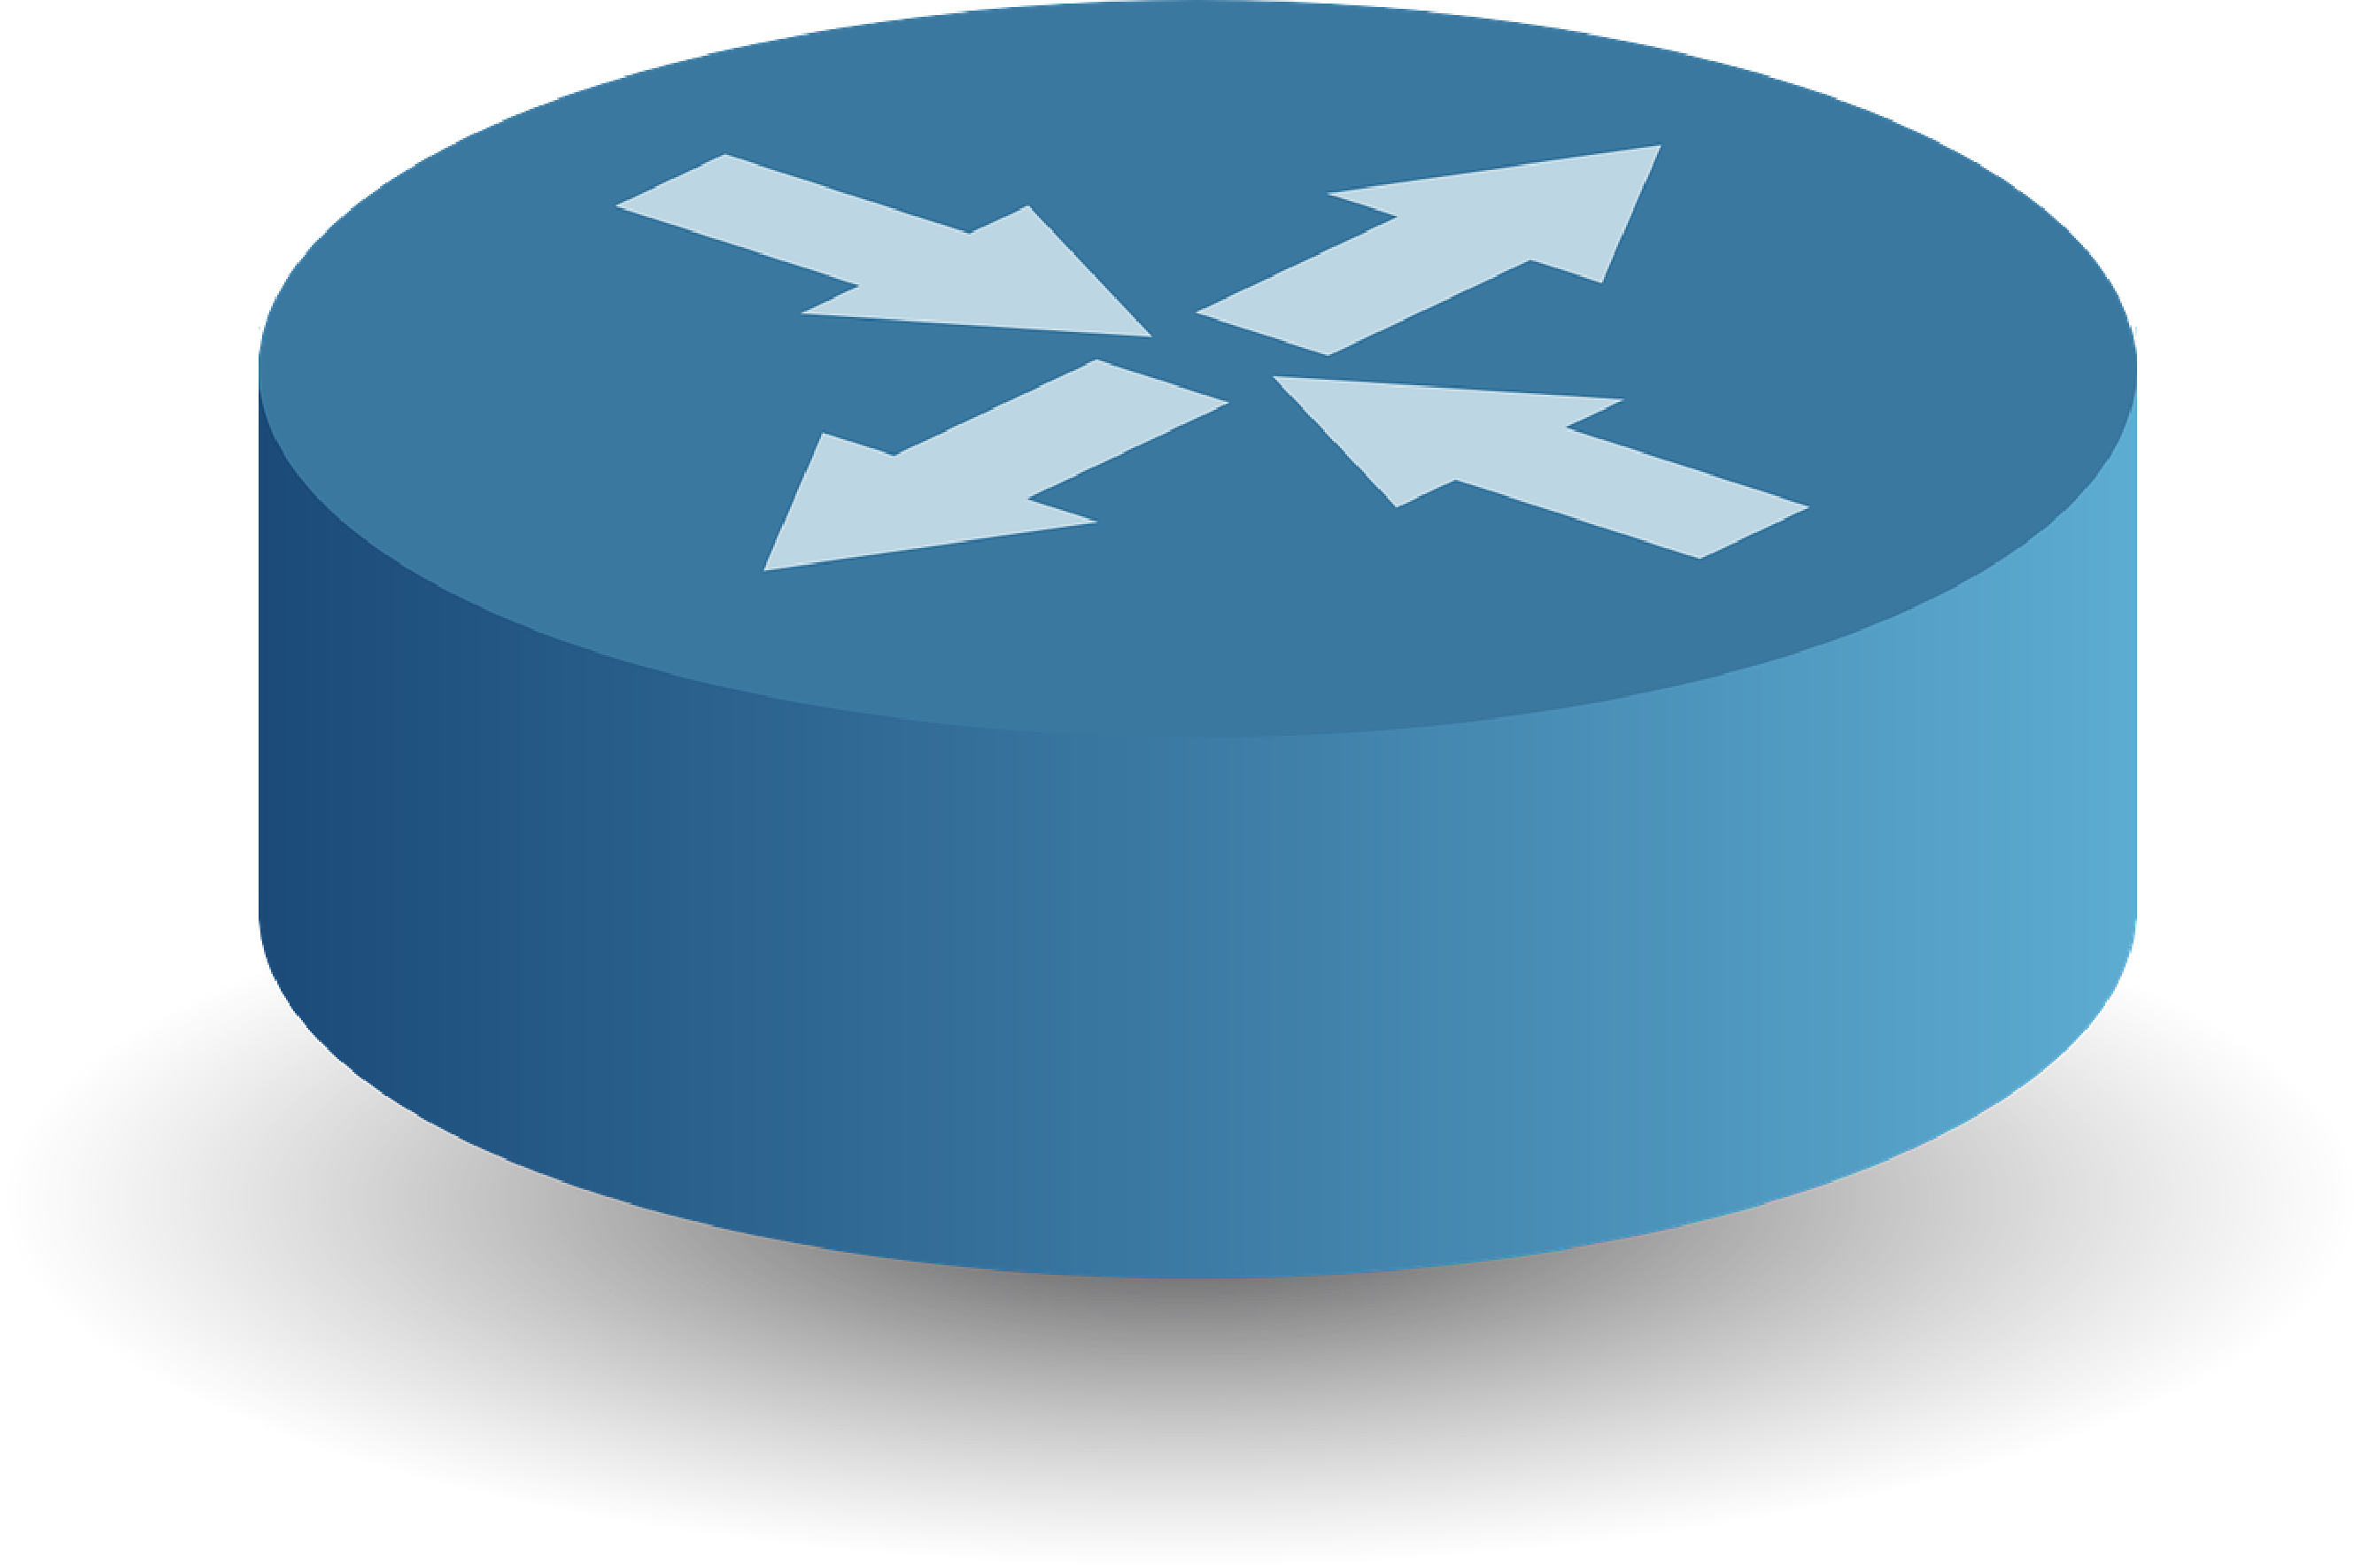
\includegraphics[width=52.5pt,height=52.5pt]{figures/router-29825_1280.pdf}};
%Image [id:dp9413637243735231] 
\draw (459,216.5) node  {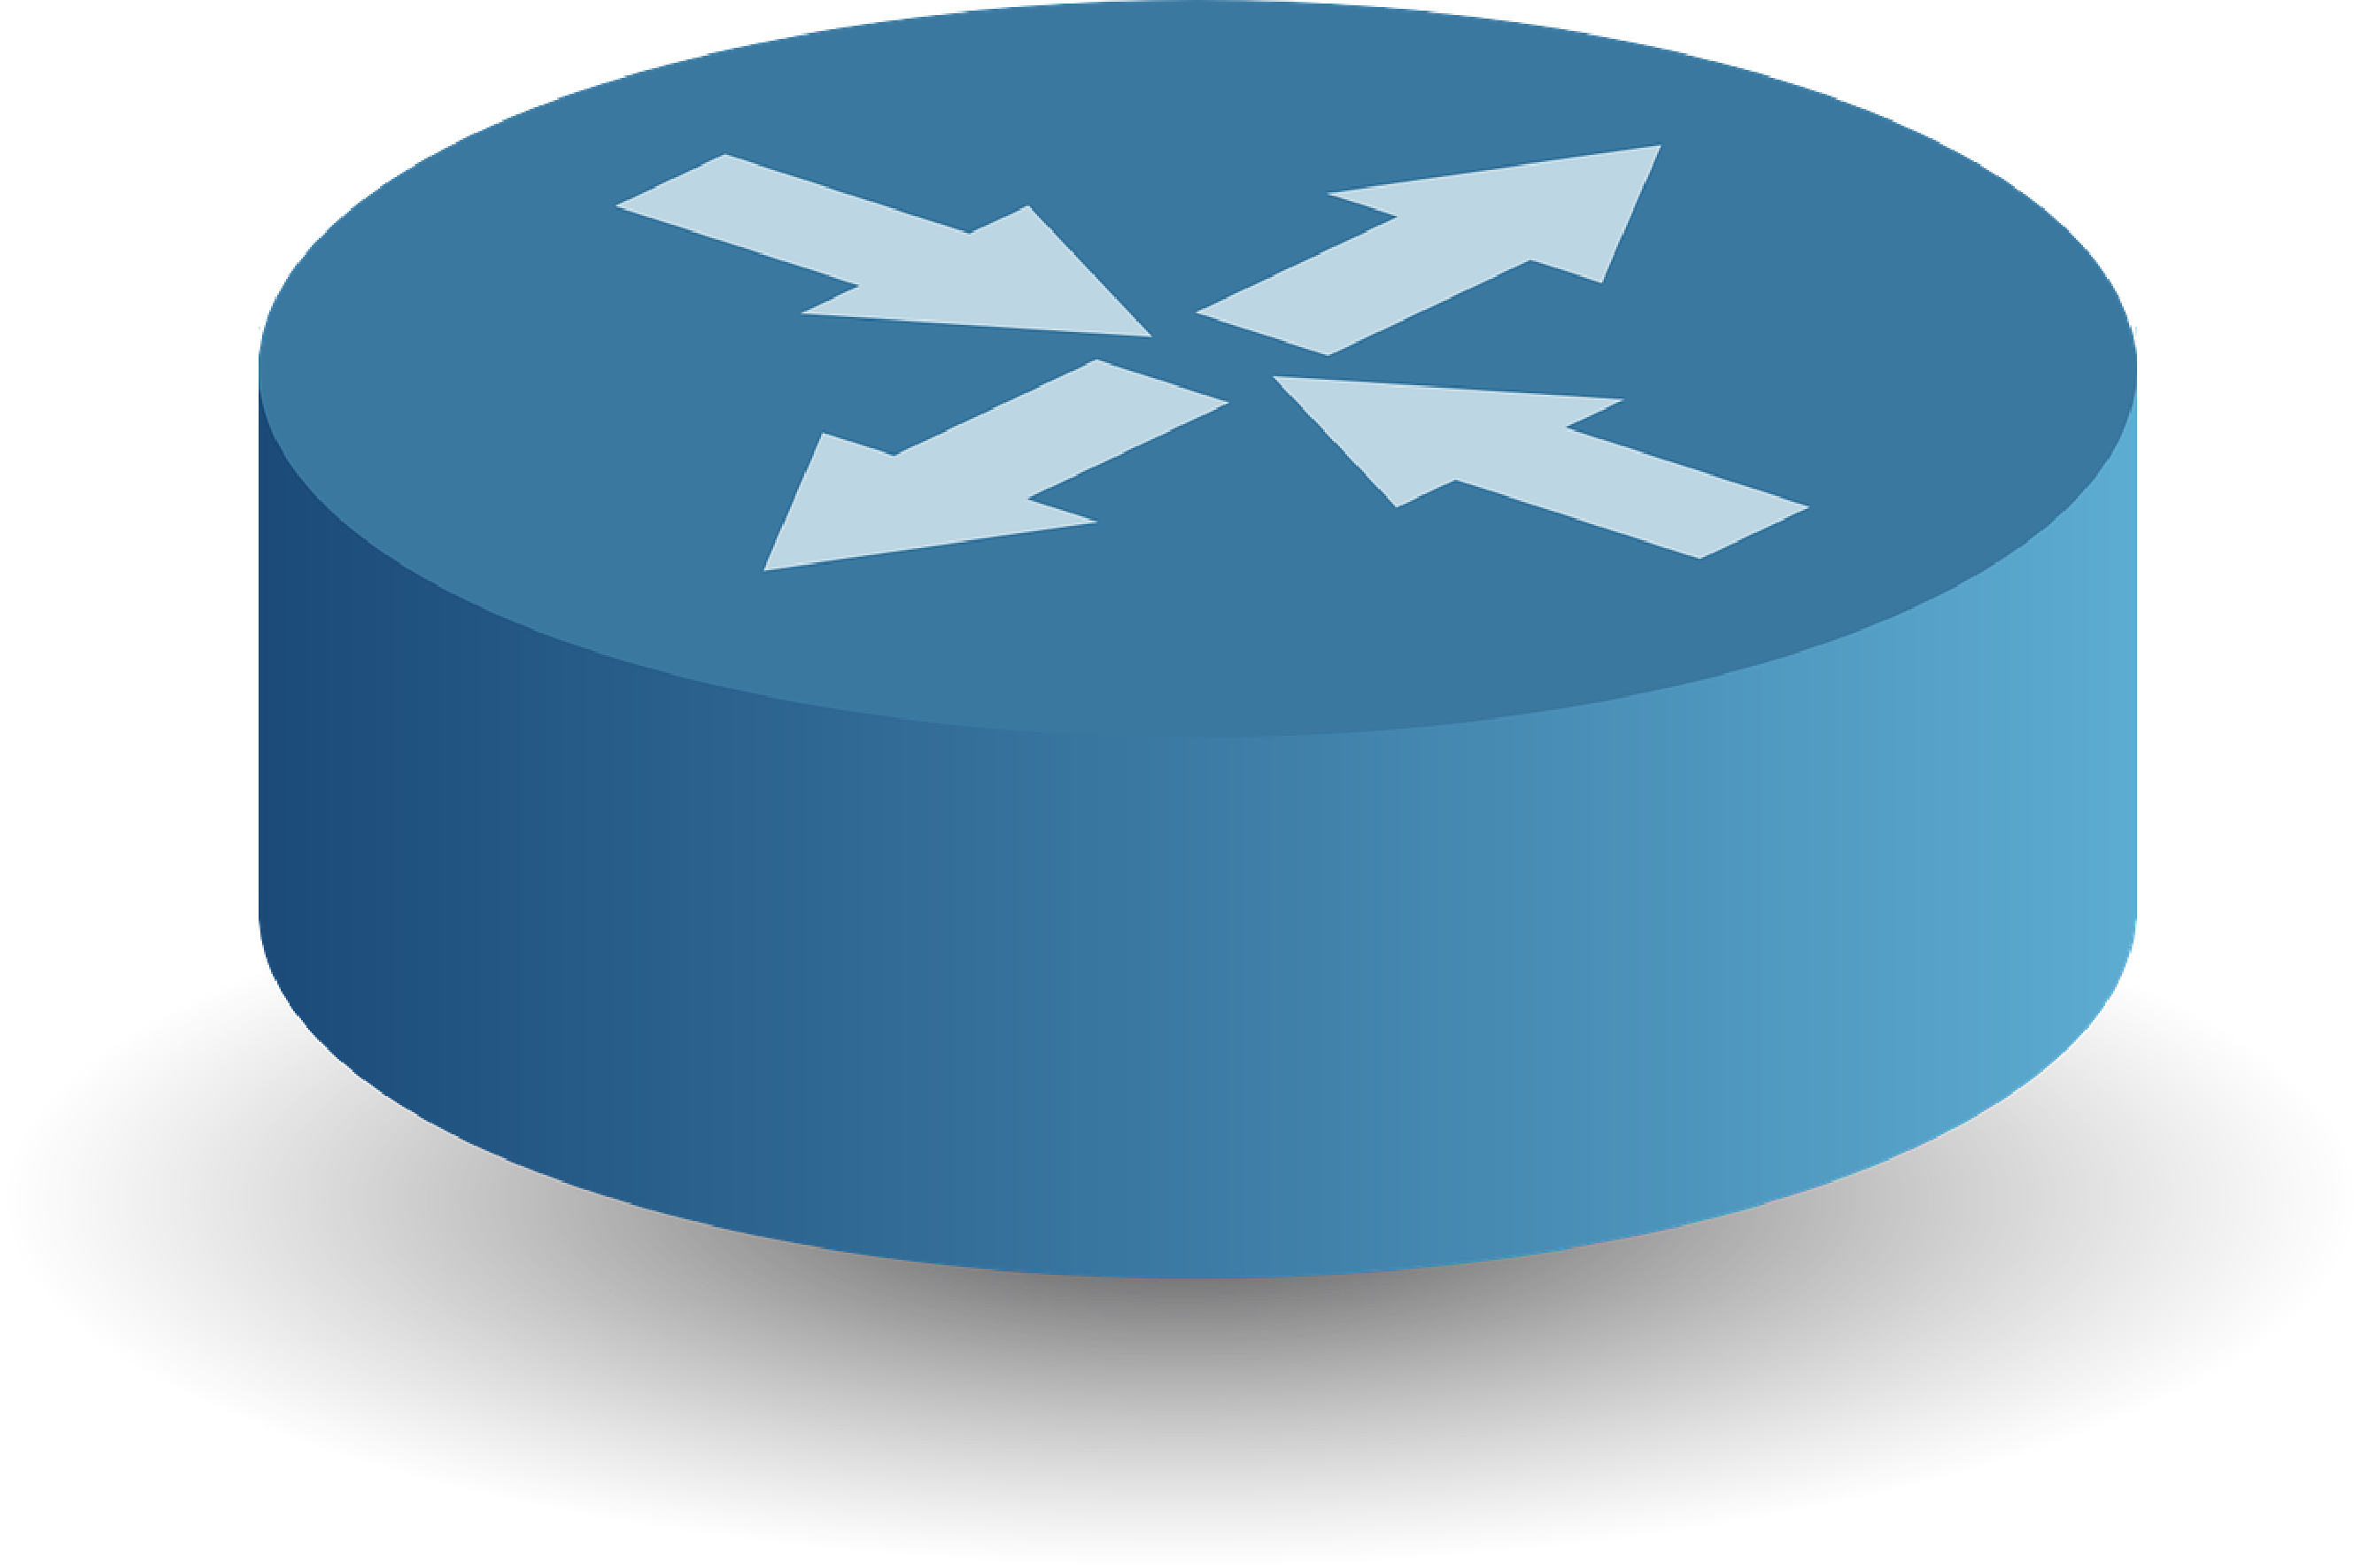
\includegraphics[width=52.5pt,height=52.5pt]{figures/router-29825_1280.pdf}};
%Image [id:dp785651084861142] 
\draw (281,216.5) node  {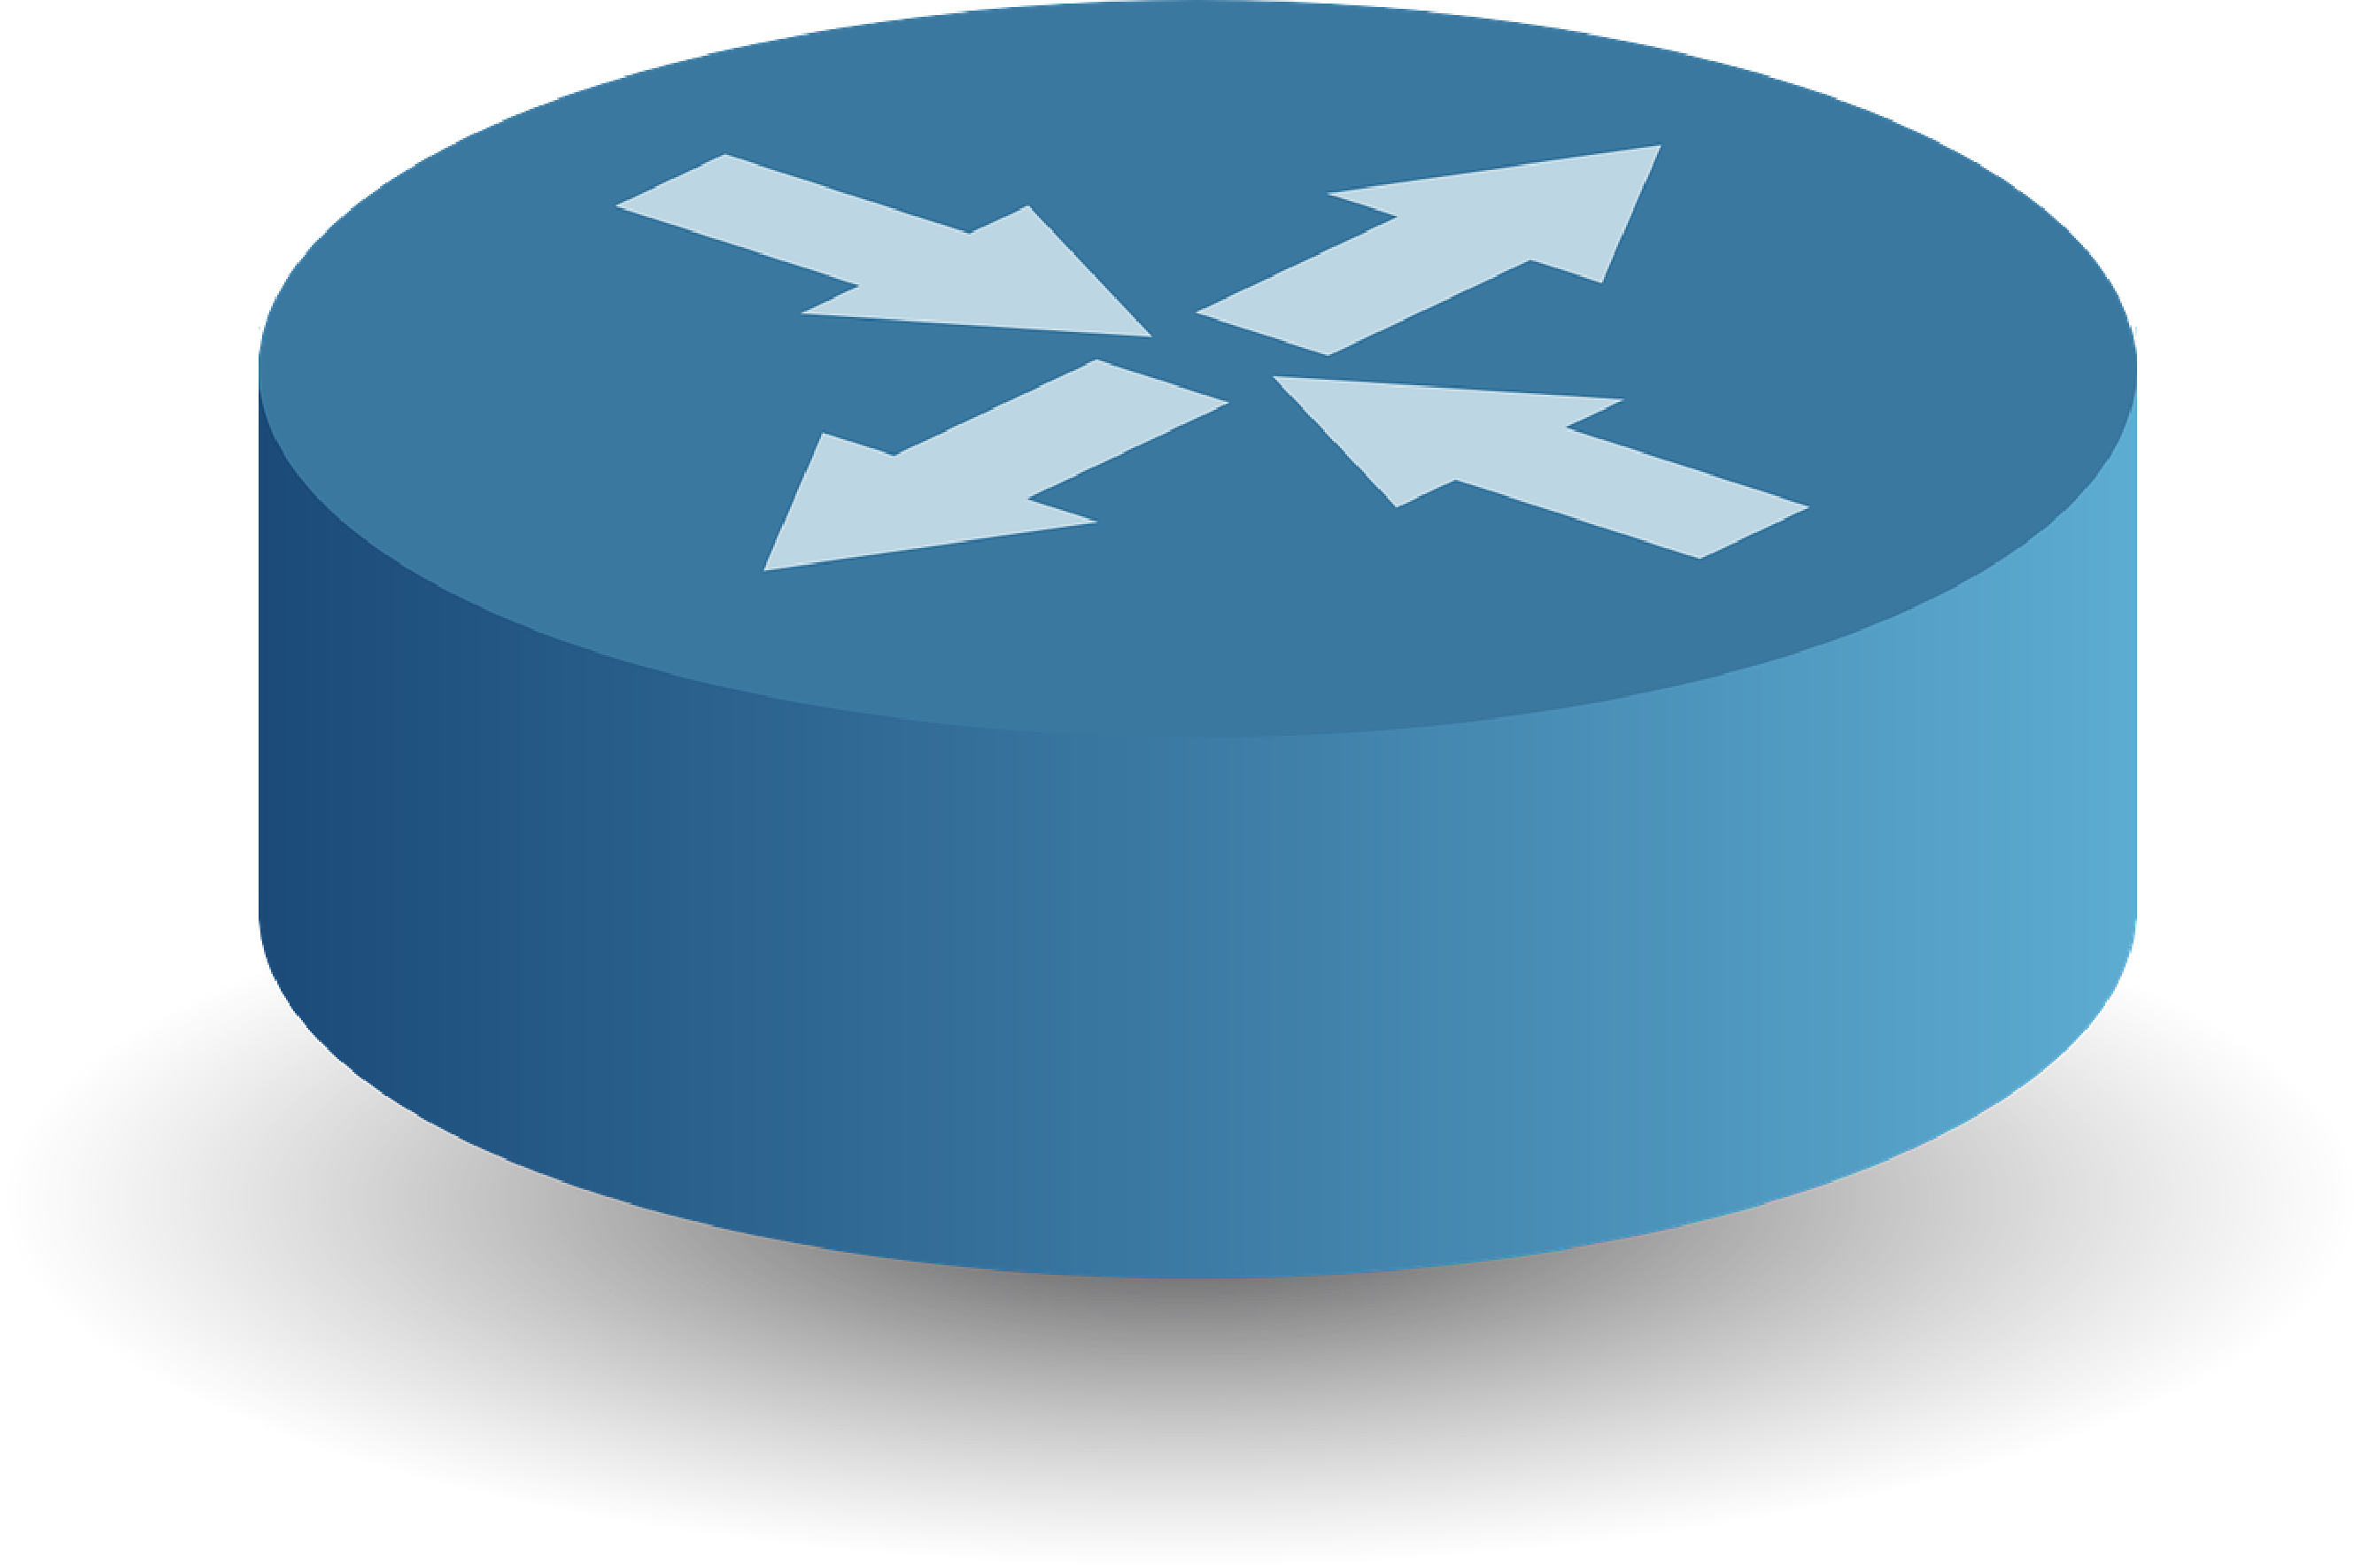
\includegraphics[width=52.5pt,height=52.5pt]{figures/router-29825_1280.pdf}};
%Rounded Rect [id:dp3607470454038808] 
\draw  [fill={rgb, 255:red, 255; green, 248; blue, 177 }  ,fill opacity=1 ] (6,89.8) .. controls (6,68.37) and (23.37,51) .. (44.8,51) -- (176.2,51) .. controls (197.63,51) and (215,68.37) .. (215,89.8) -- (215,206.2) .. controls (215,227.63) and (197.63,245) .. (176.2,245) -- (44.8,245) .. controls (23.37,245) and (6,227.63) .. (6,206.2) -- cycle ;

%Straight Lines [id:da6281461745789373] 
\draw [line width=1.5]  [dash pattern={on 1.69pt off 2.76pt}]  (45,103.33) -- (120,203.33) ;


%Straight Lines [id:da1553743343202807] 
\draw [line width=1.5]  [dash pattern={on 1.69pt off 2.76pt}]  (45,103.33) -- (181,104.33) ;


%Straight Lines [id:da7040489254906964] 
\draw [line width=1.5]  [dash pattern={on 1.69pt off 2.76pt}]  (119,202.33) -- (180,103.33) ;


%Image [id:dp41322551228030835] 
\draw (42.5,118) node  {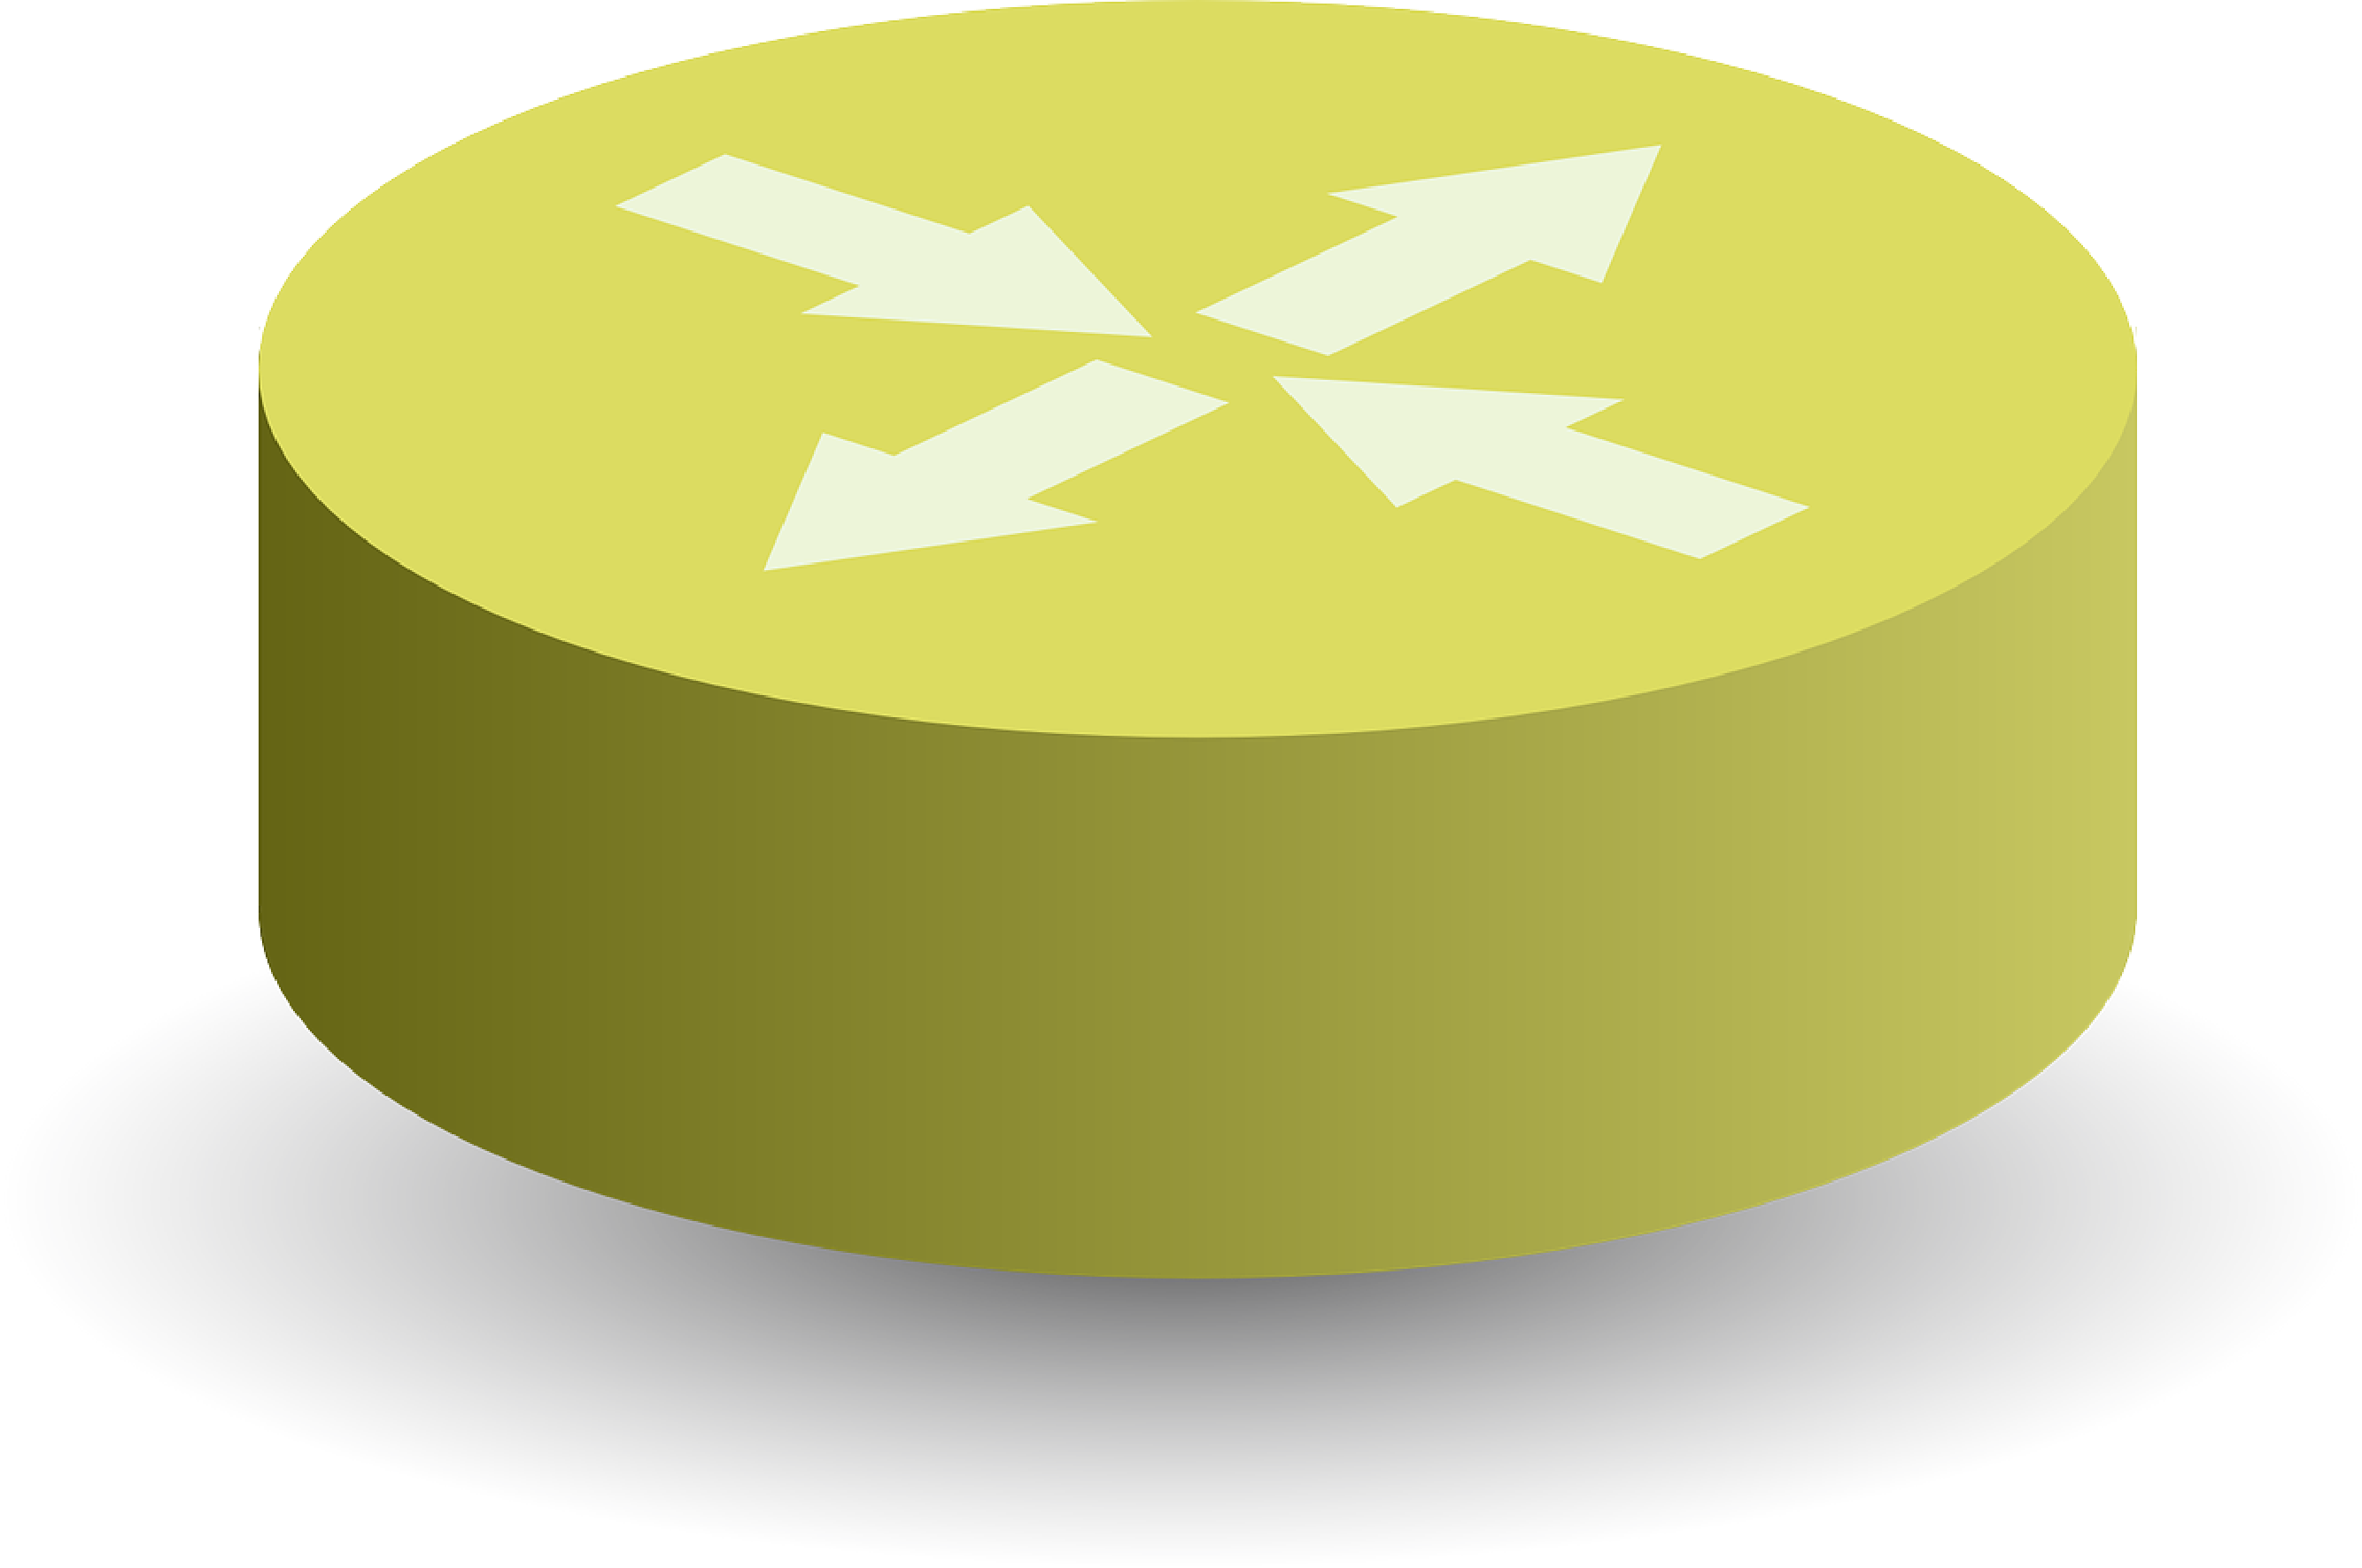
\includegraphics[width=52.5pt,height=52.5pt]{figures/router-158644_1280.pdf}};
%Image [id:dp16387001457338324] 
\draw (177.5,118) node  {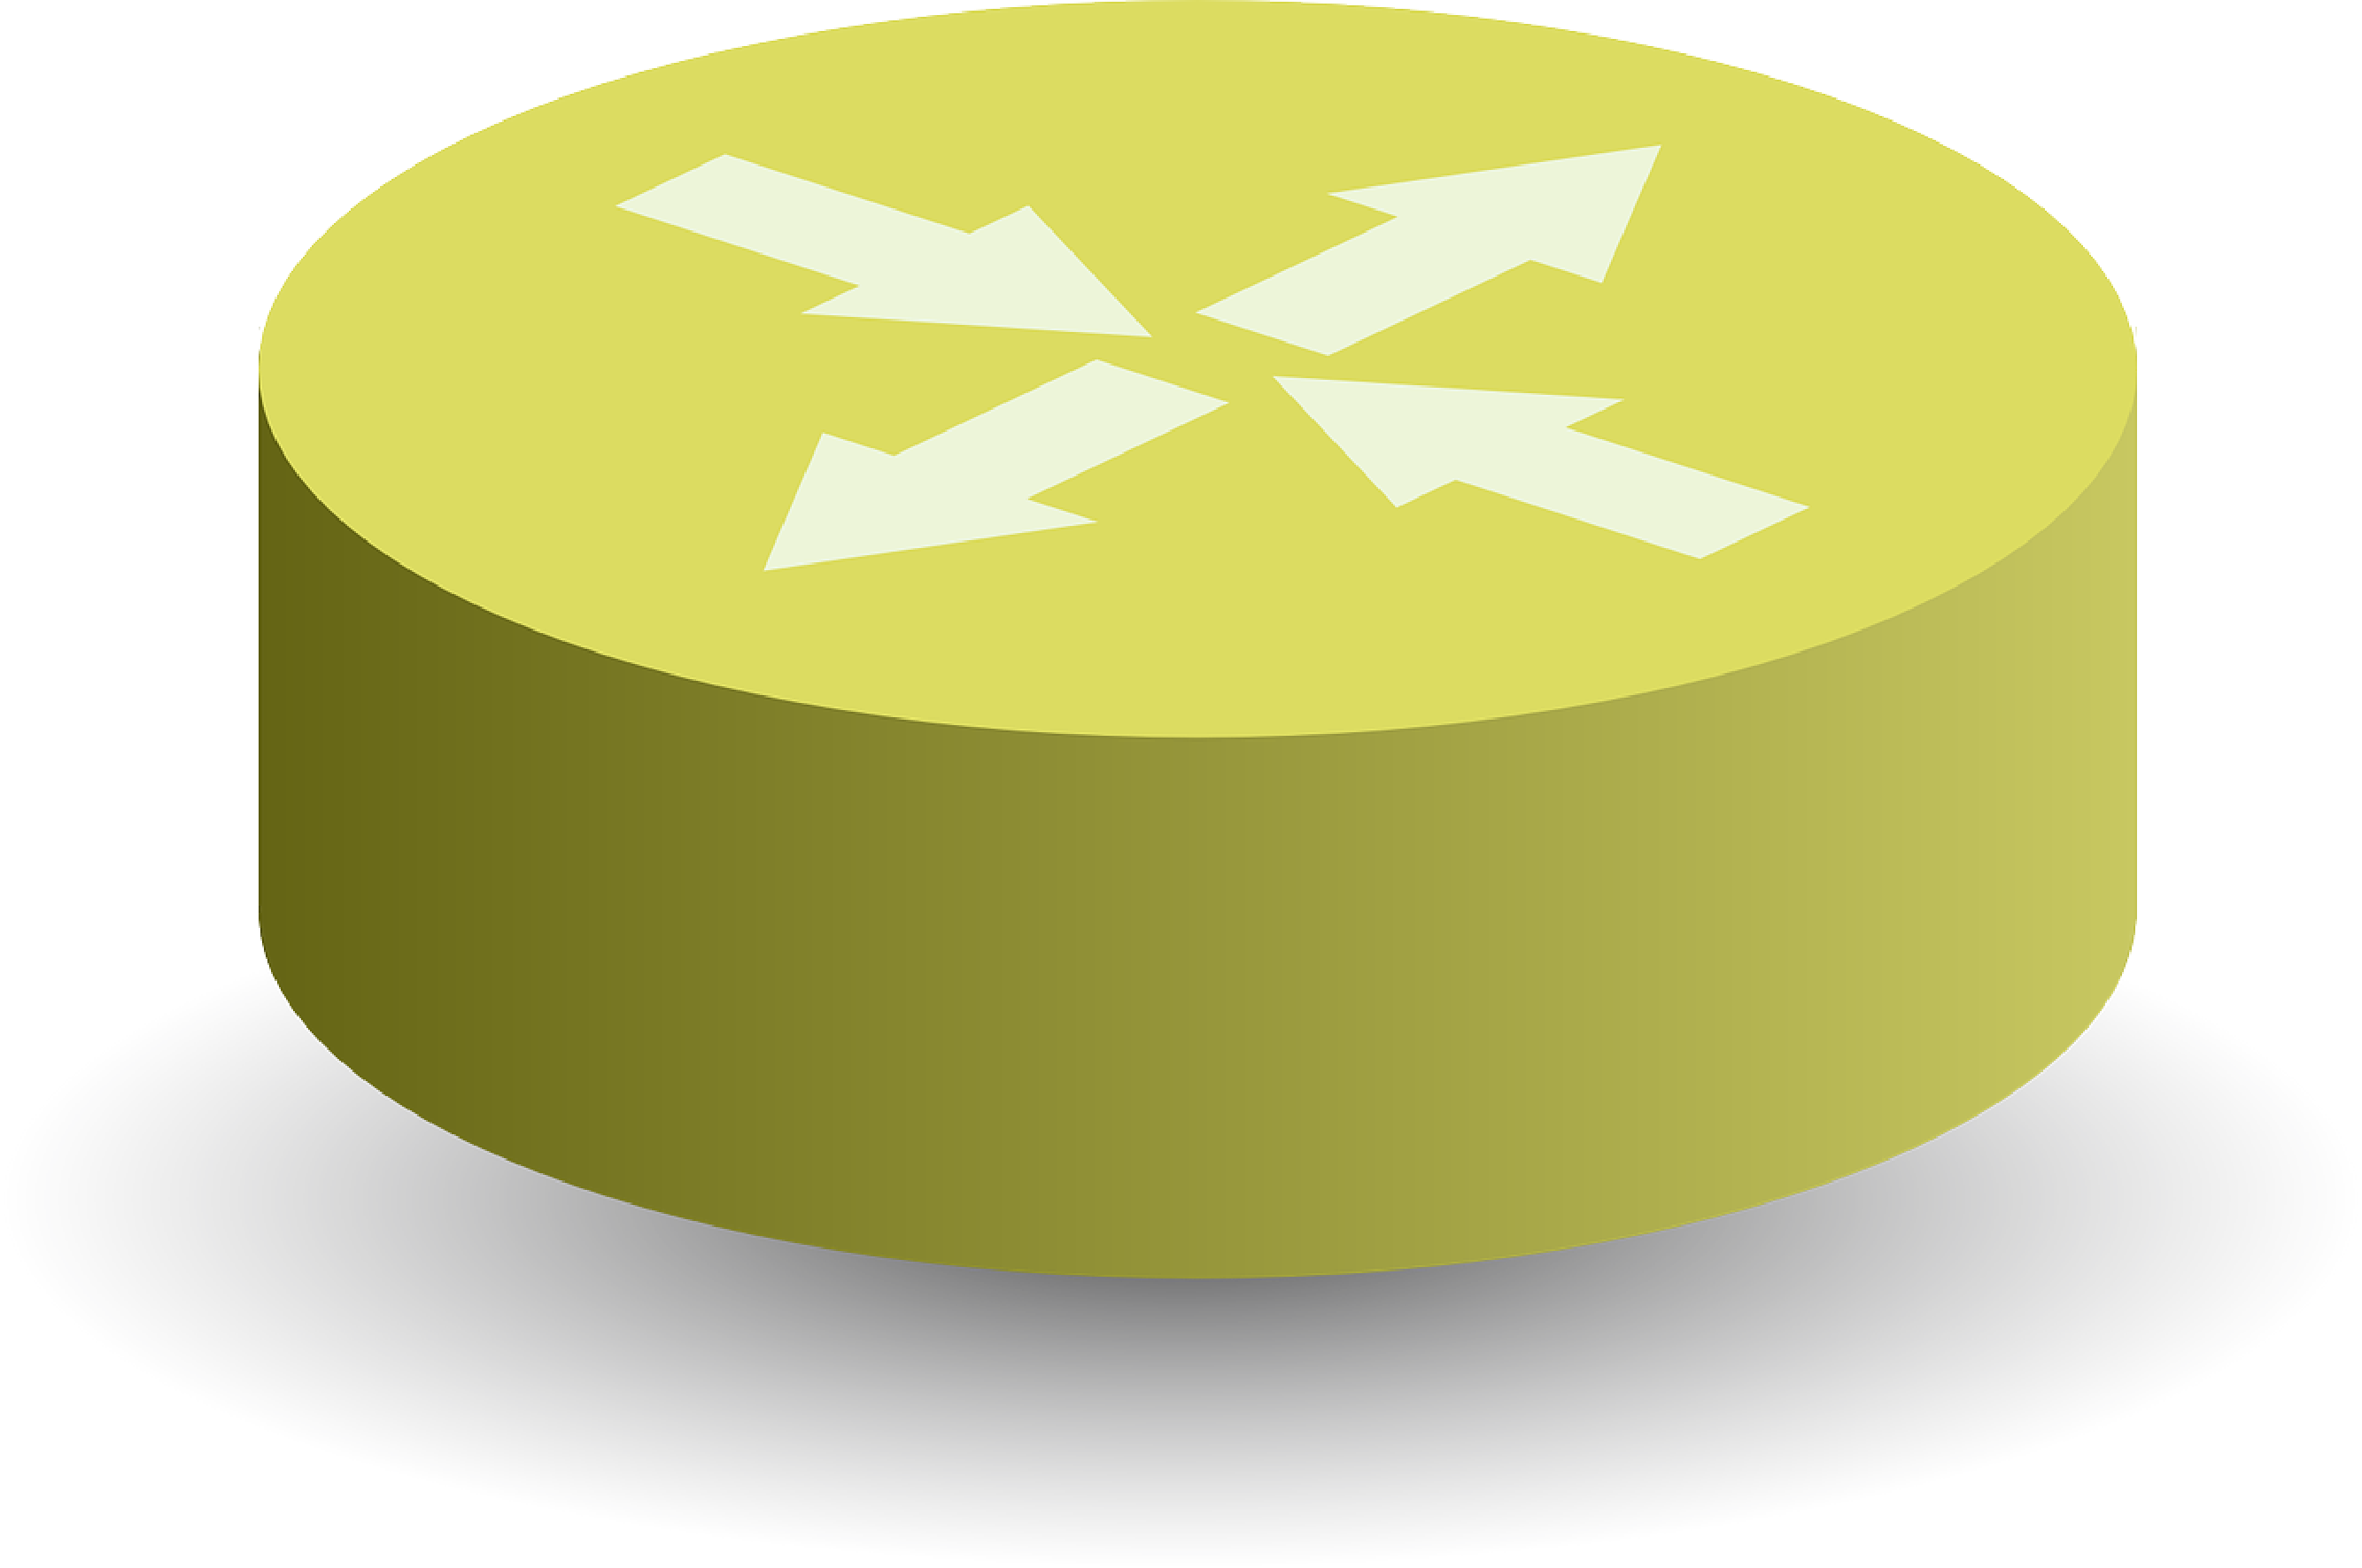
\includegraphics[width=52.5pt,height=52.5pt]{figures/router-158644_1280.pdf}};
%Image [id:dp1012276528015783] 
\draw (111.5,209.5) node  {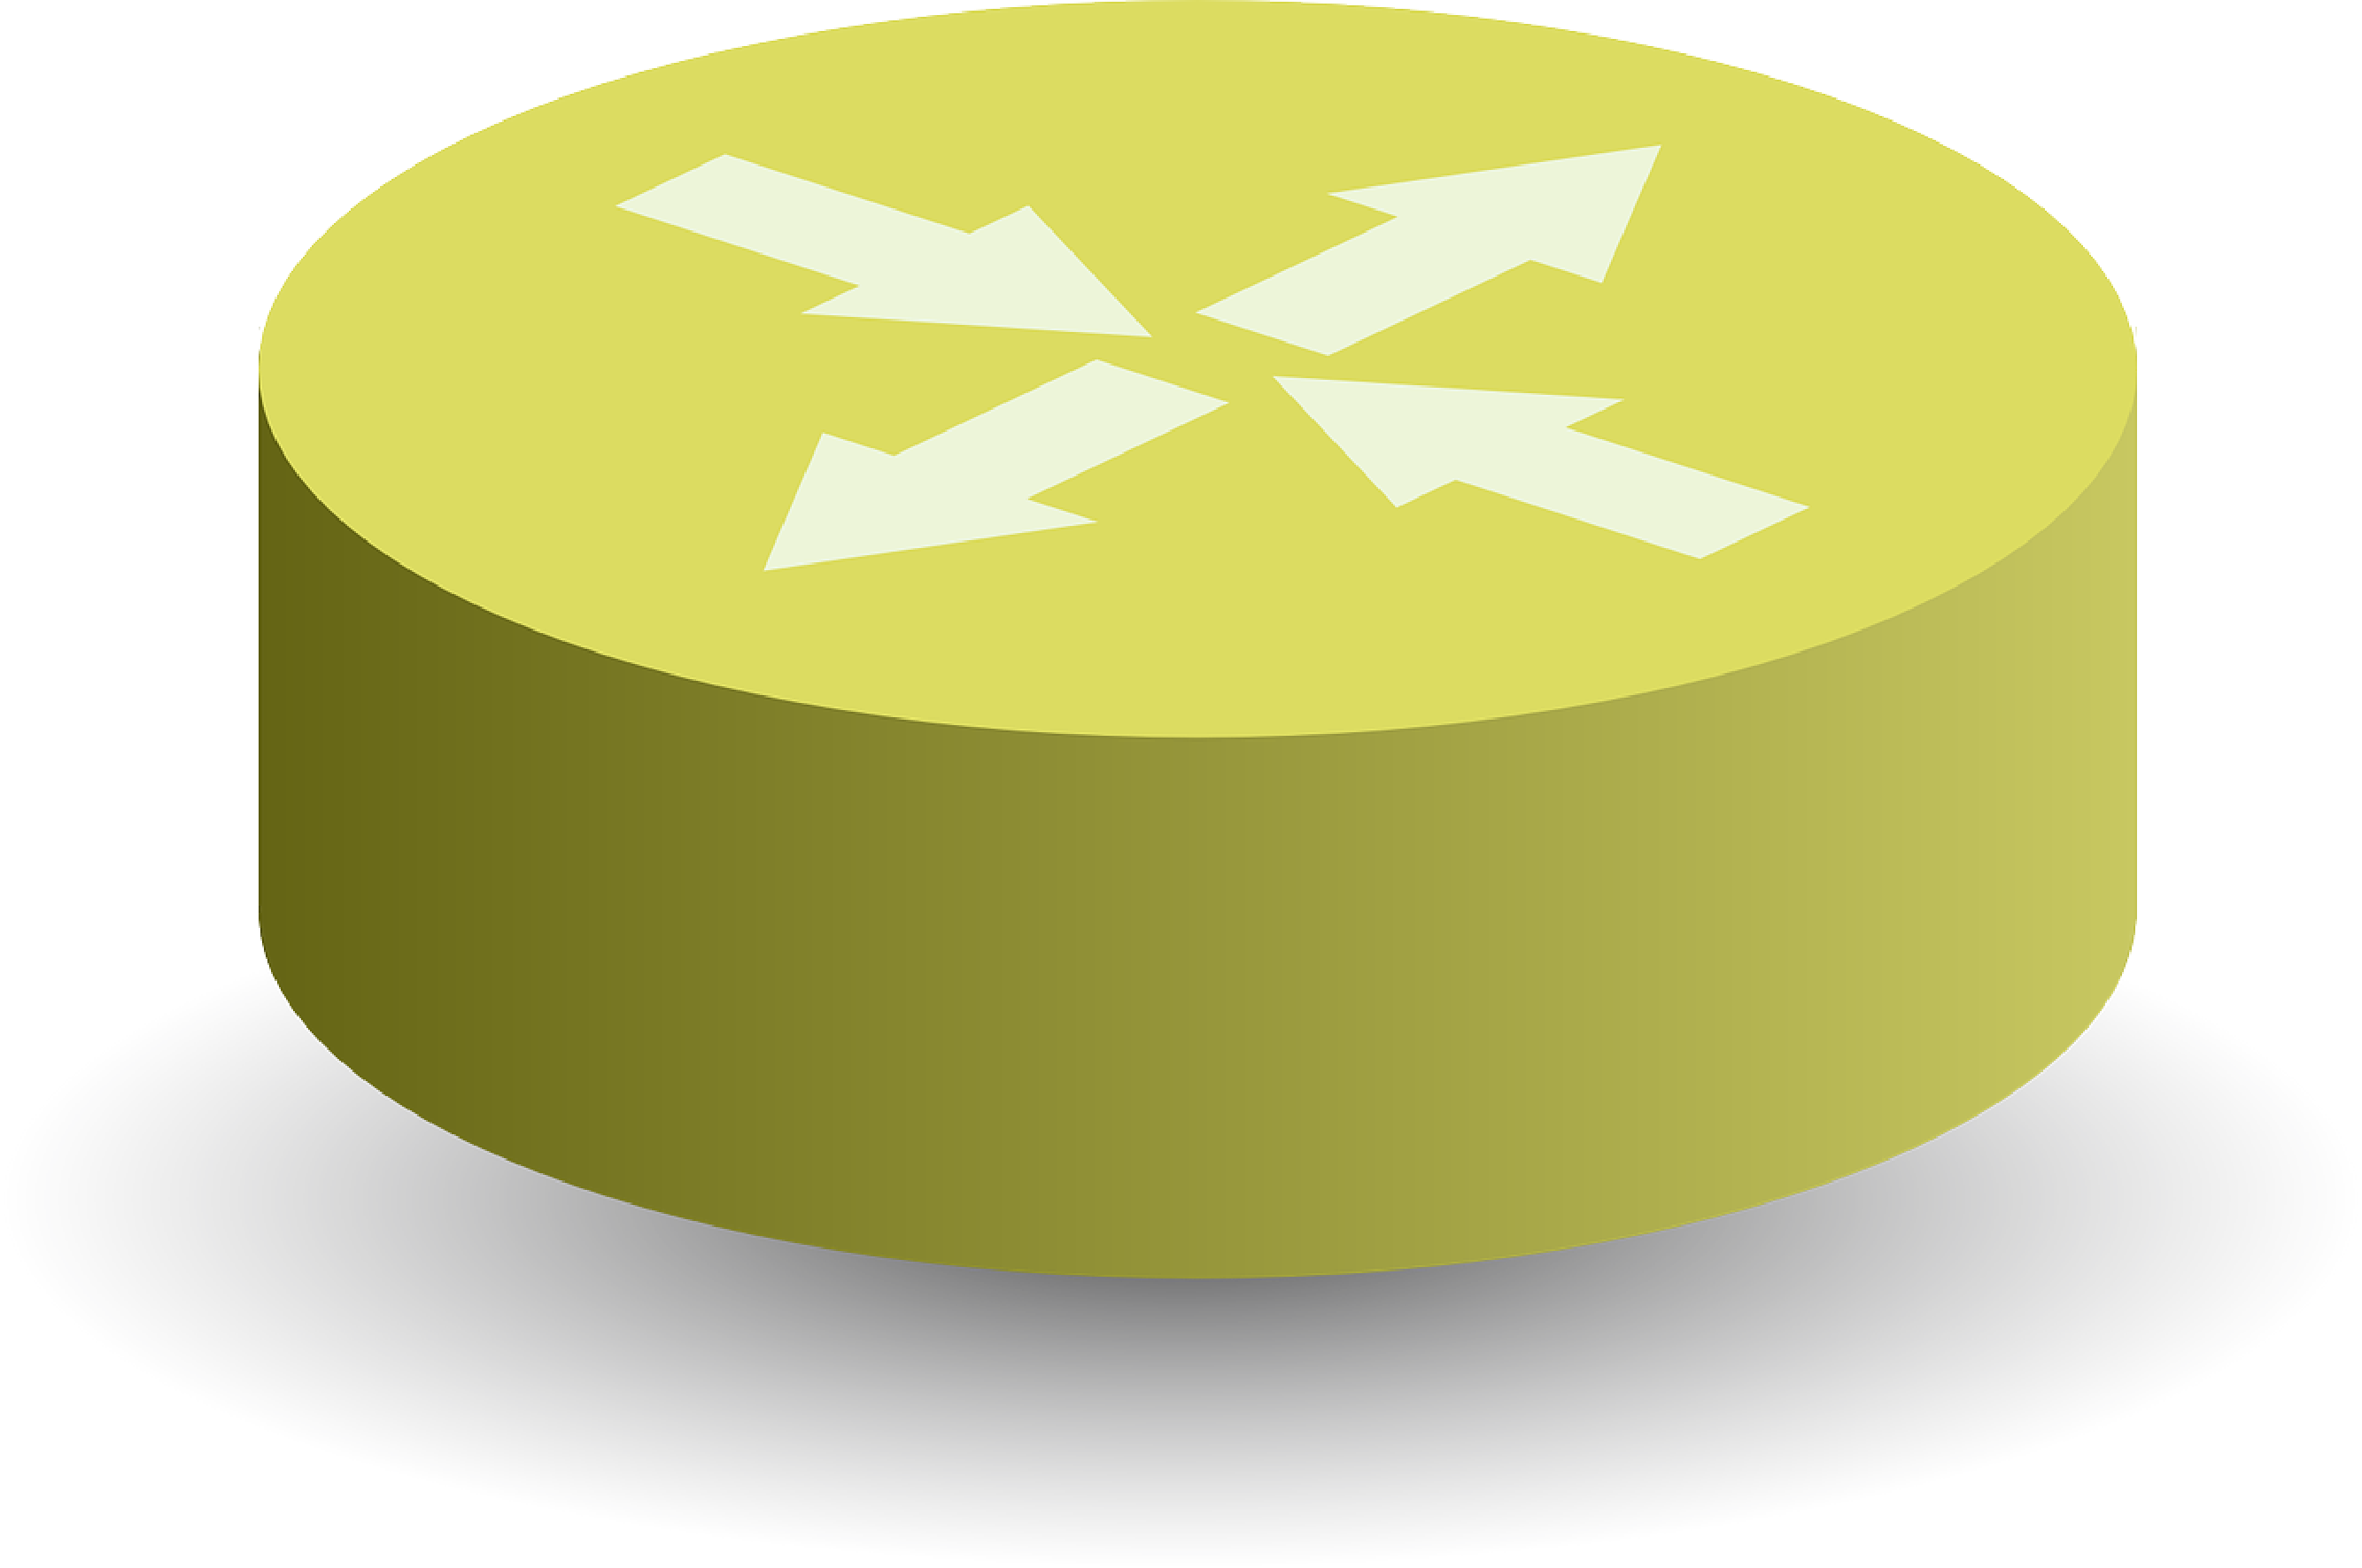
\includegraphics[width=52.5pt,height=52.5pt]{figures/router-158644_1280.pdf}};
%Straight Lines [id:da10827340921387374] 
\draw    (67,469.33) -- (180,428.33) ;


%Straight Lines [id:da02465044628511004] 
\draw    (67,469.33) -- (182,526.33) ;


%Straight Lines [id:da7232328020483667] 
\draw    (179,526.33) -- (177,428.33) ;


%Straight Lines [id:da6335138571596731] 
\draw    (440,530.33) -- (438,432.33) ;


%Straight Lines [id:da5081473547182844] 
\draw    (186,435.33) -- (462,436.33) ;


%Straight Lines [id:da5273919871085183] 
\draw    (185,530.33) -- (461,531.33) ;


%Image [id:dp10904051335047615] 
\draw (68,484.5) node  {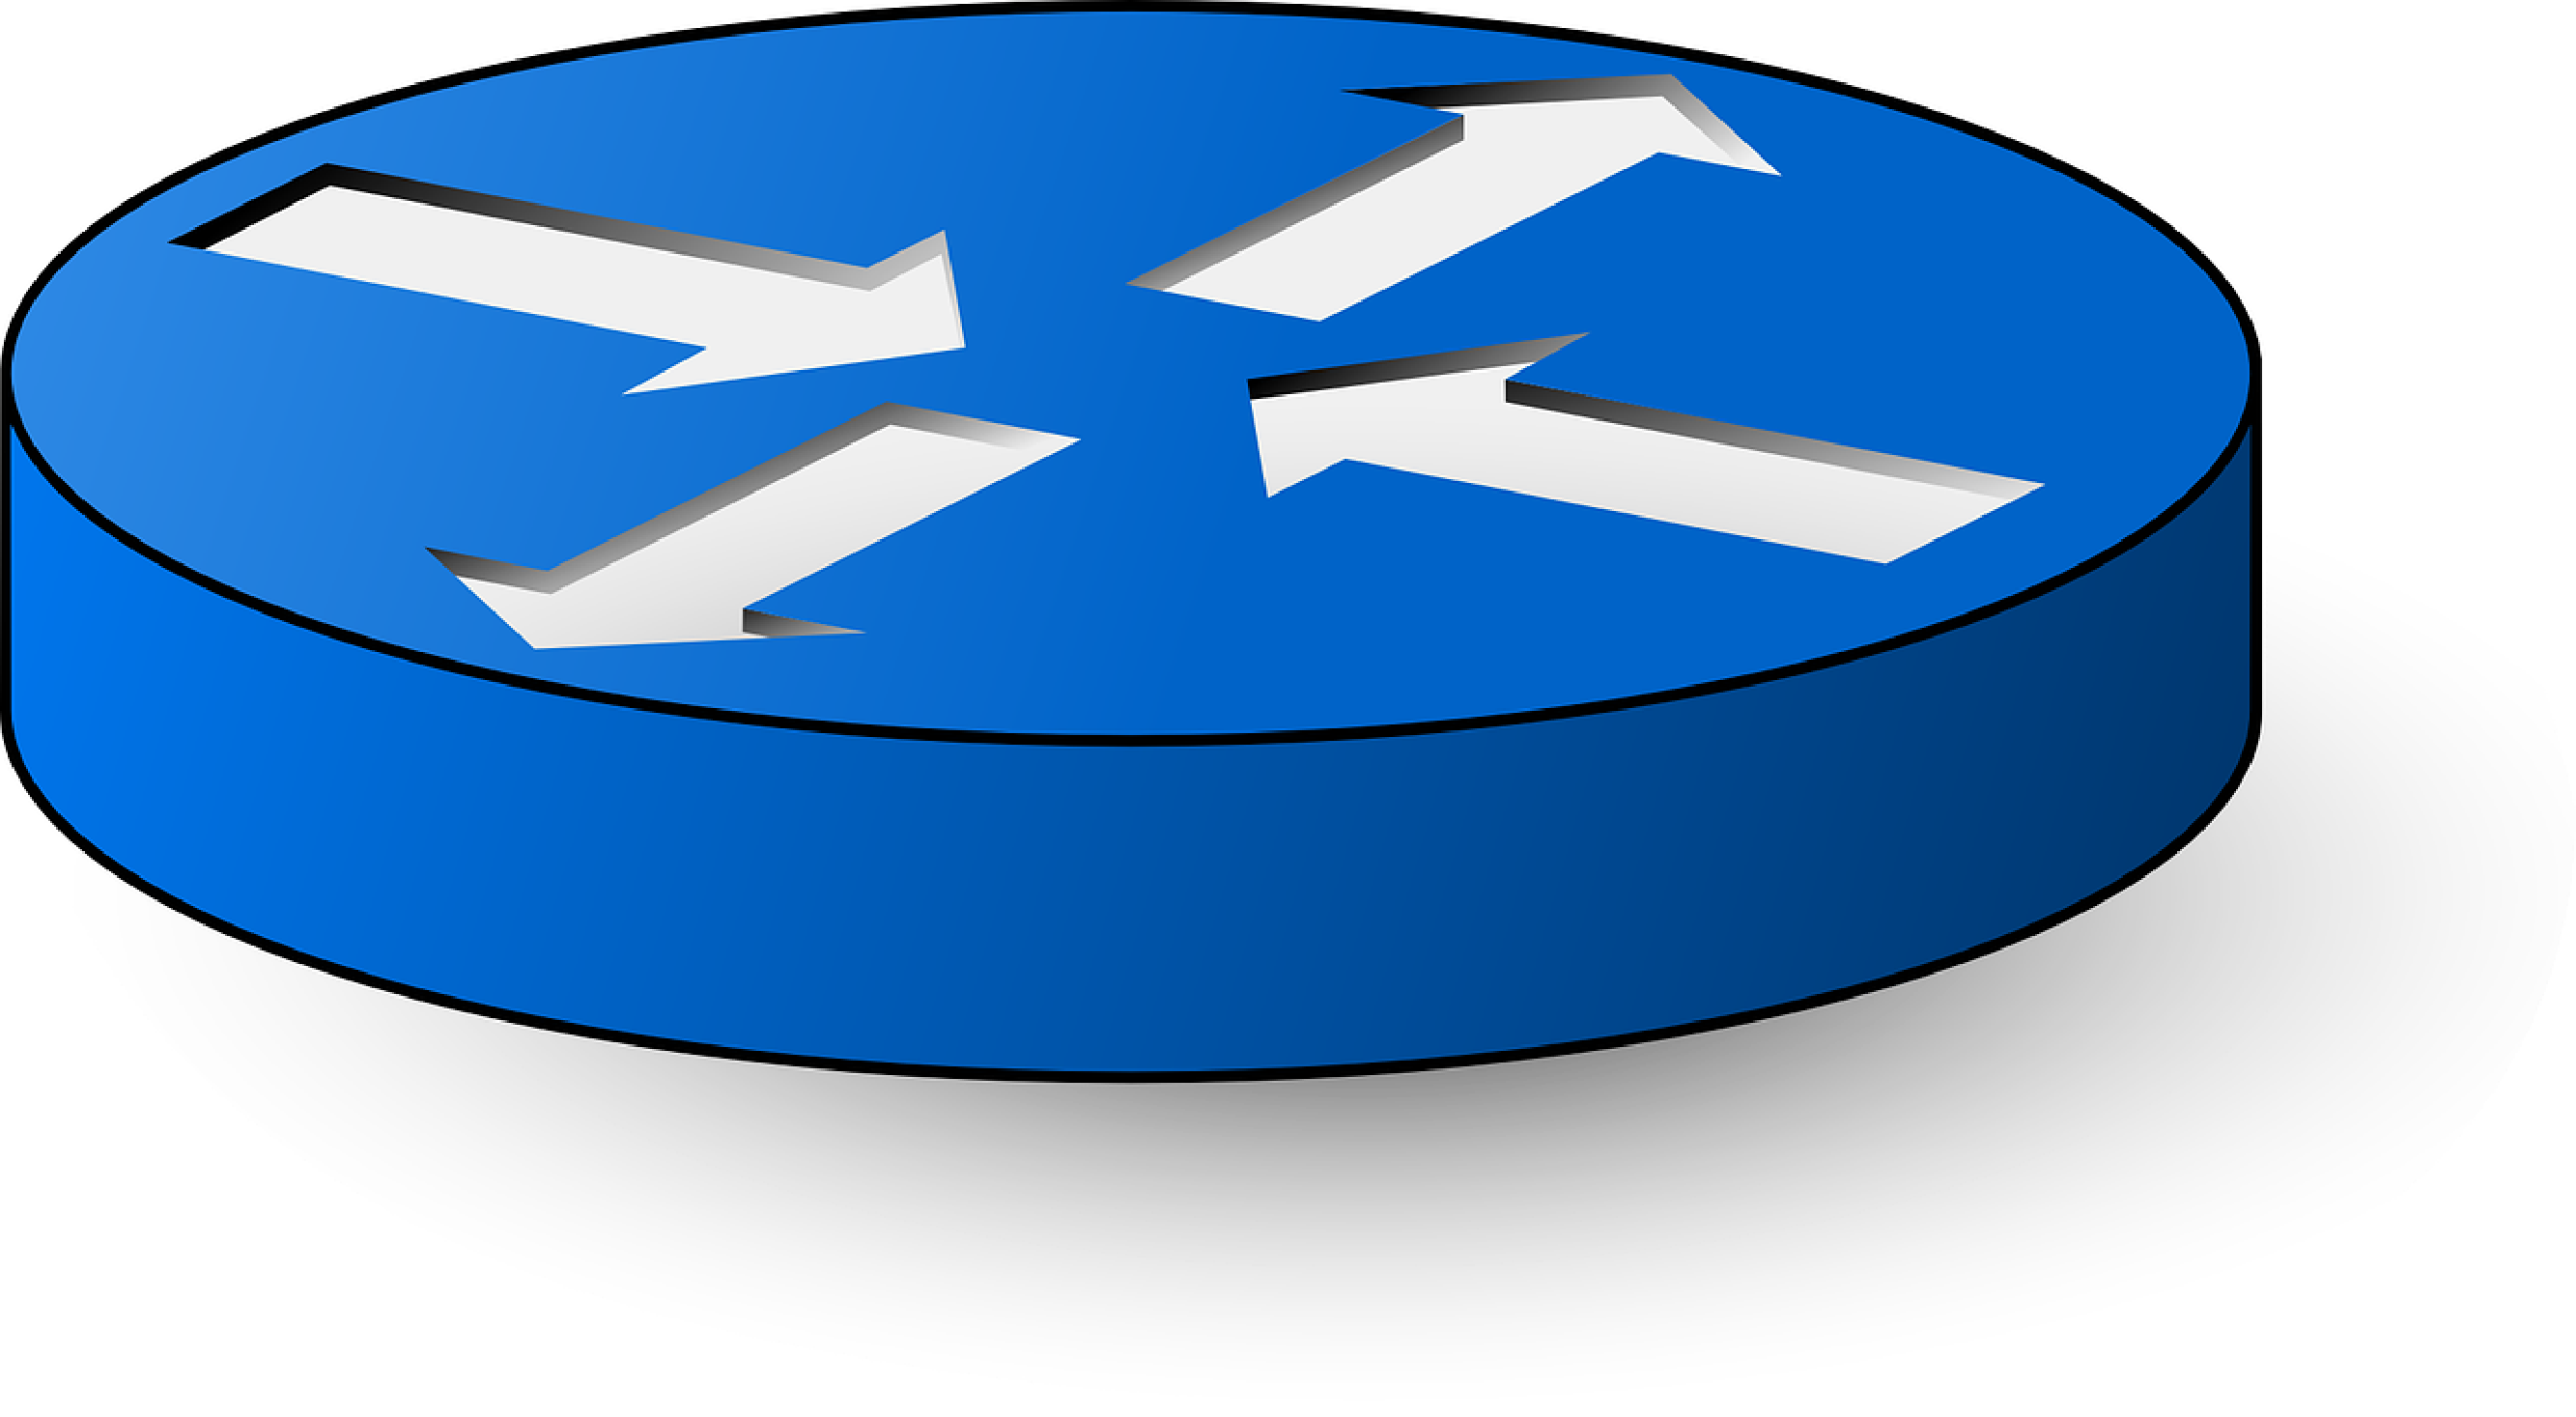
\includegraphics[width=52.5pt,height=52.5pt]{figures/router-30140_1280.pdf}};
%Image [id:dp7146163070755307] 
\draw (185,444.5) node  {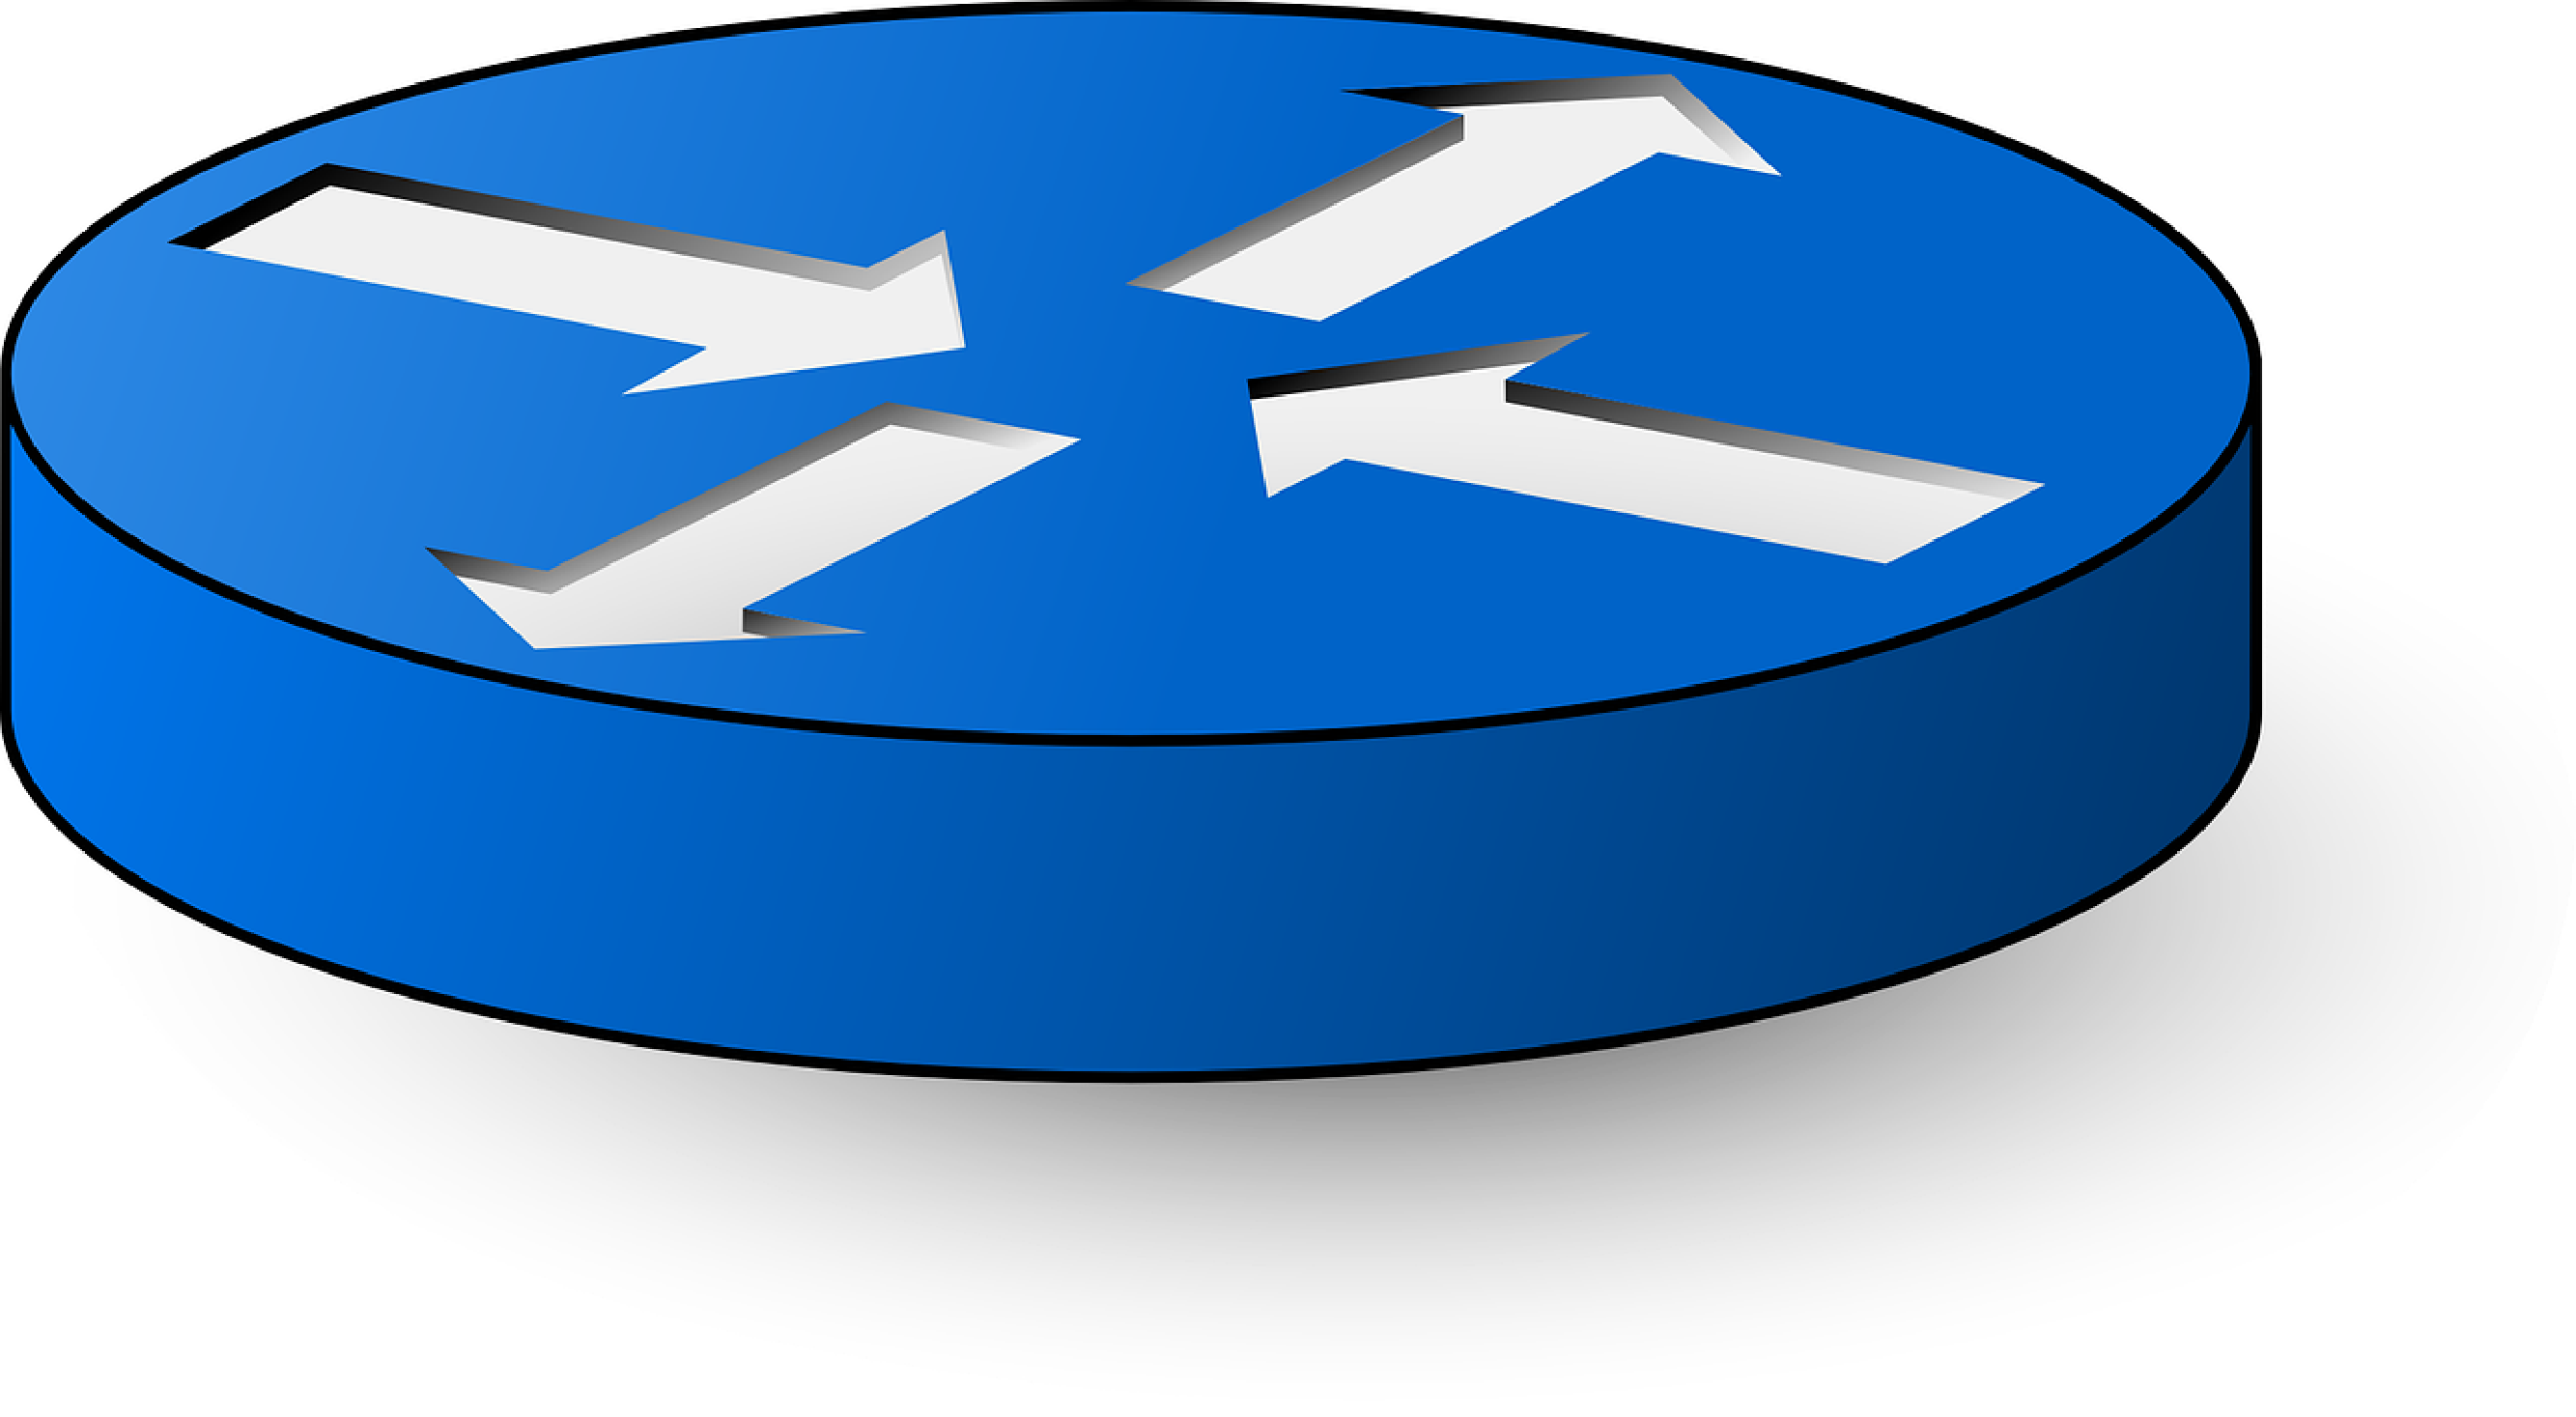
\includegraphics[width=52.5pt,height=52.5pt]{figures/router-30140_1280.pdf}};
%Image [id:dp9757131158412626] 
\draw (441.5,544.5) node  {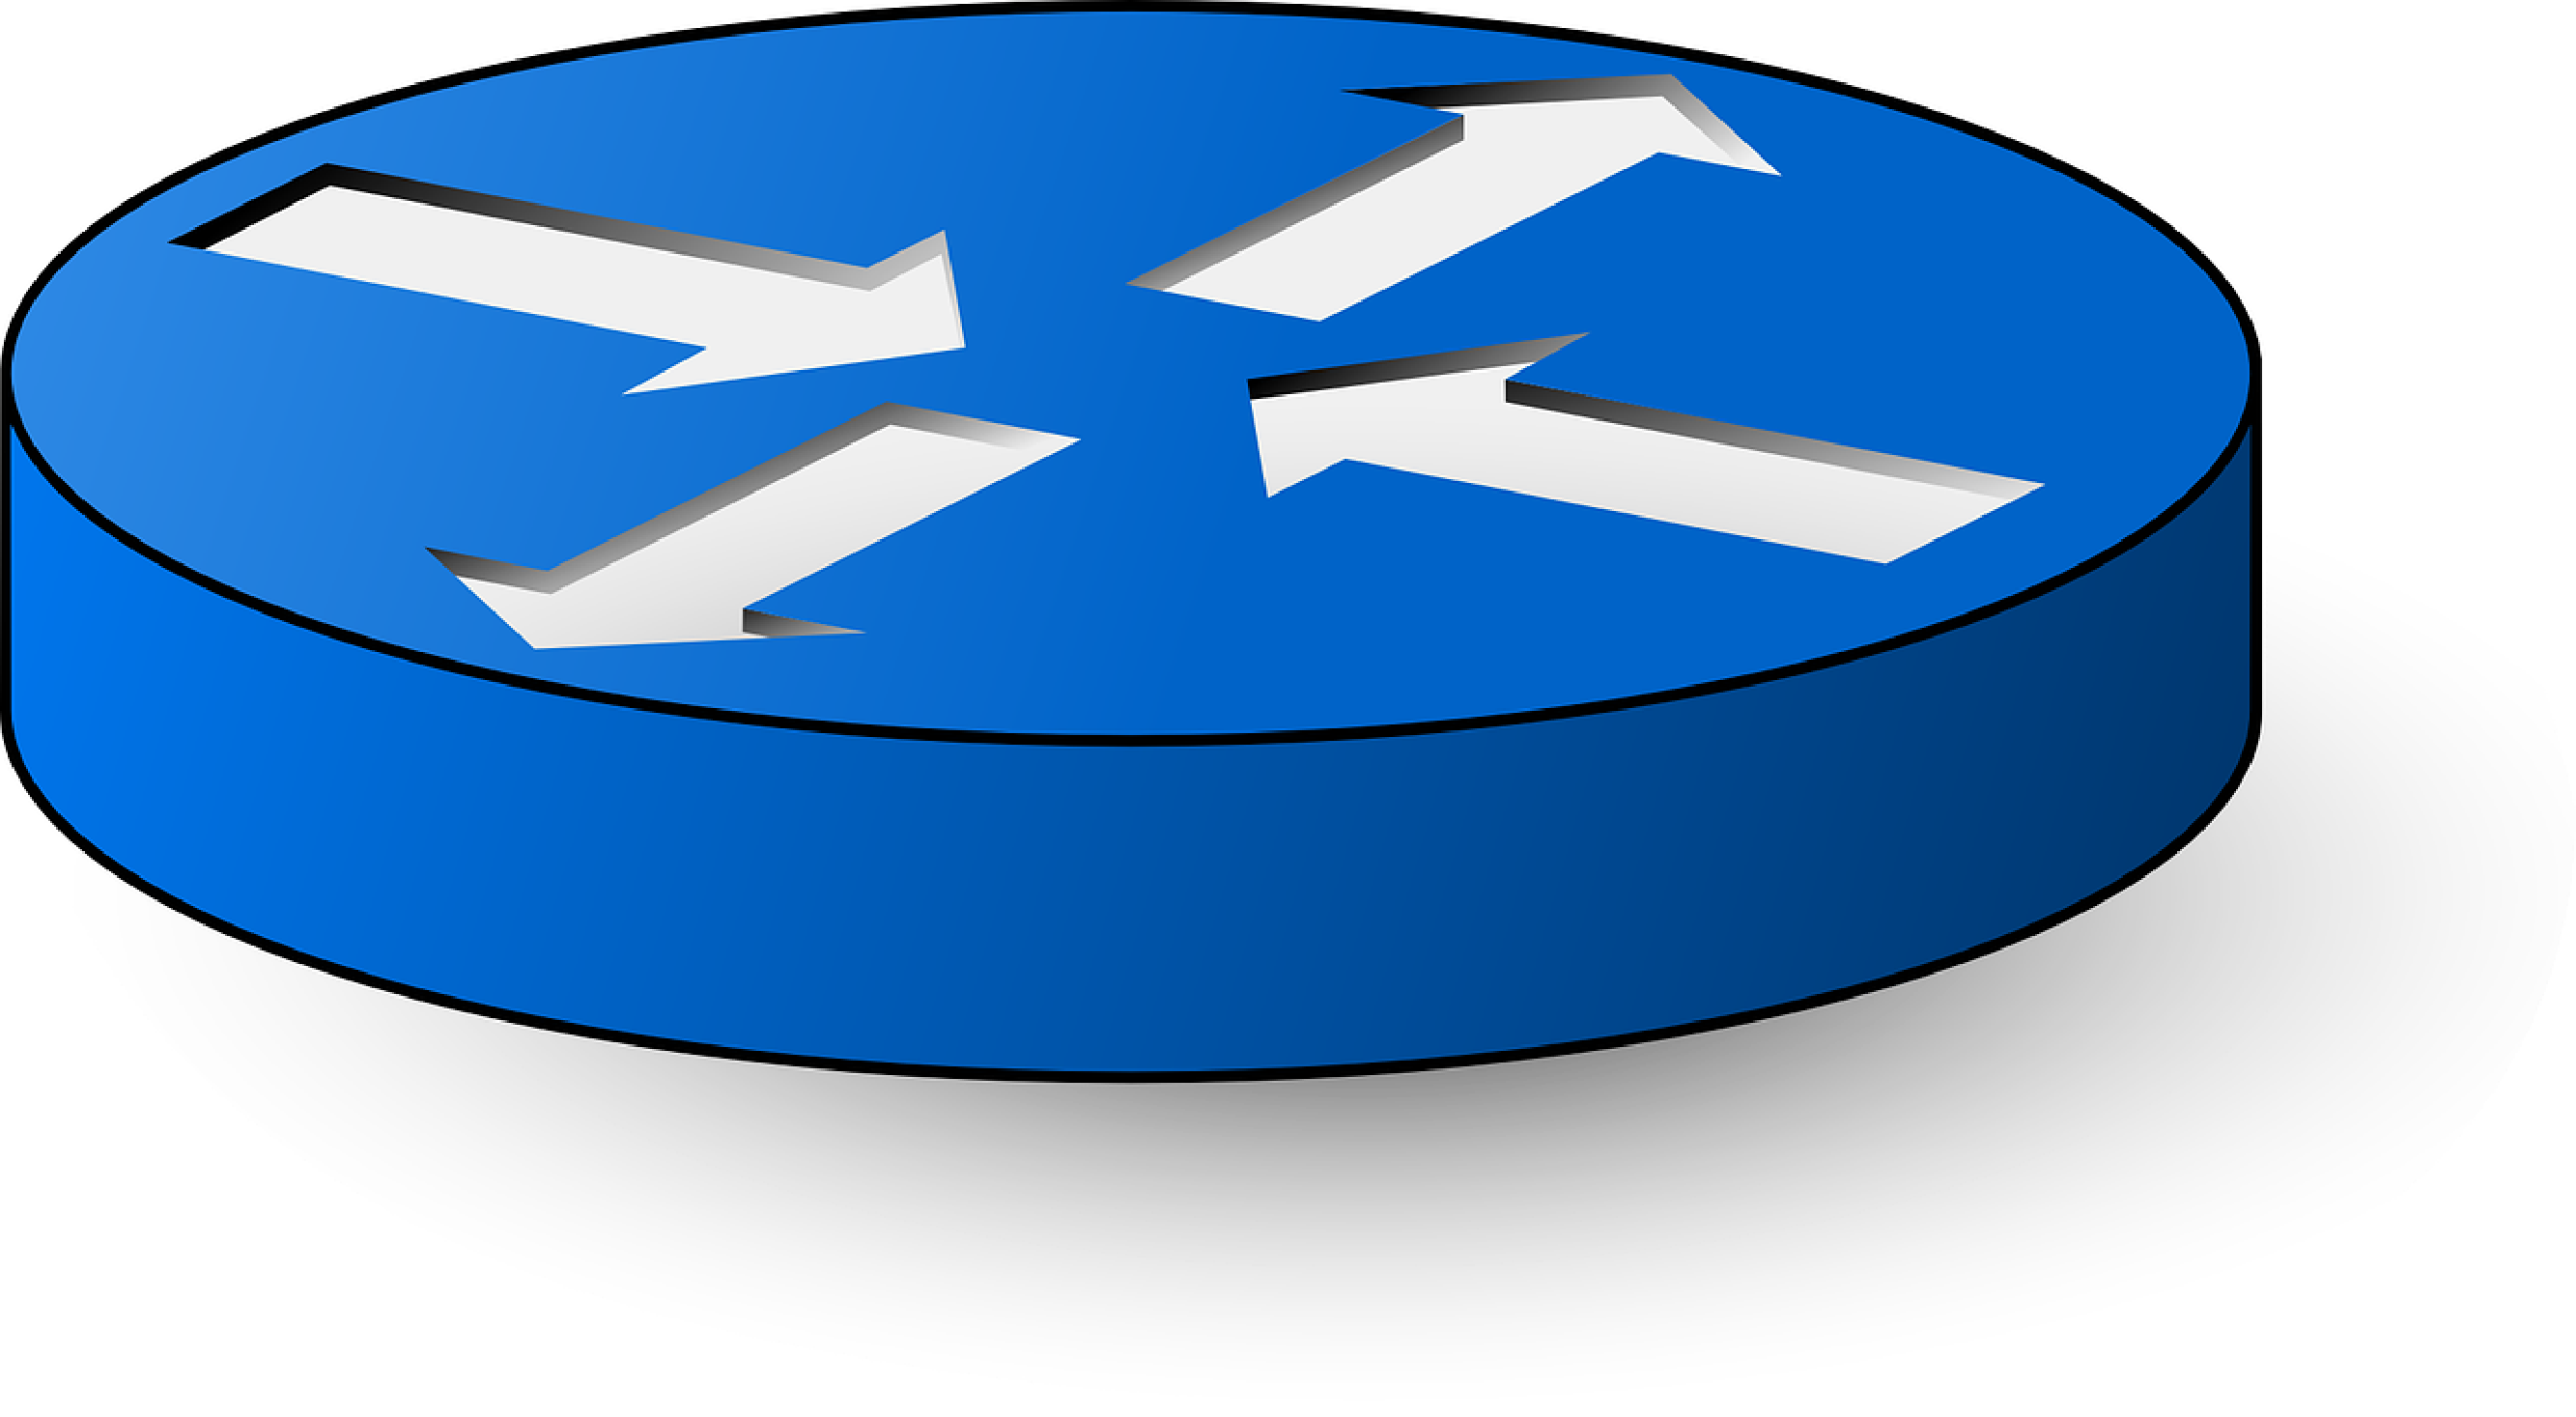
\includegraphics[width=52.5pt,height=52.5pt]{figures/router-30140_1280.pdf}};
%Image [id:dp21403253894649854] 
\draw (184,546.5) node  {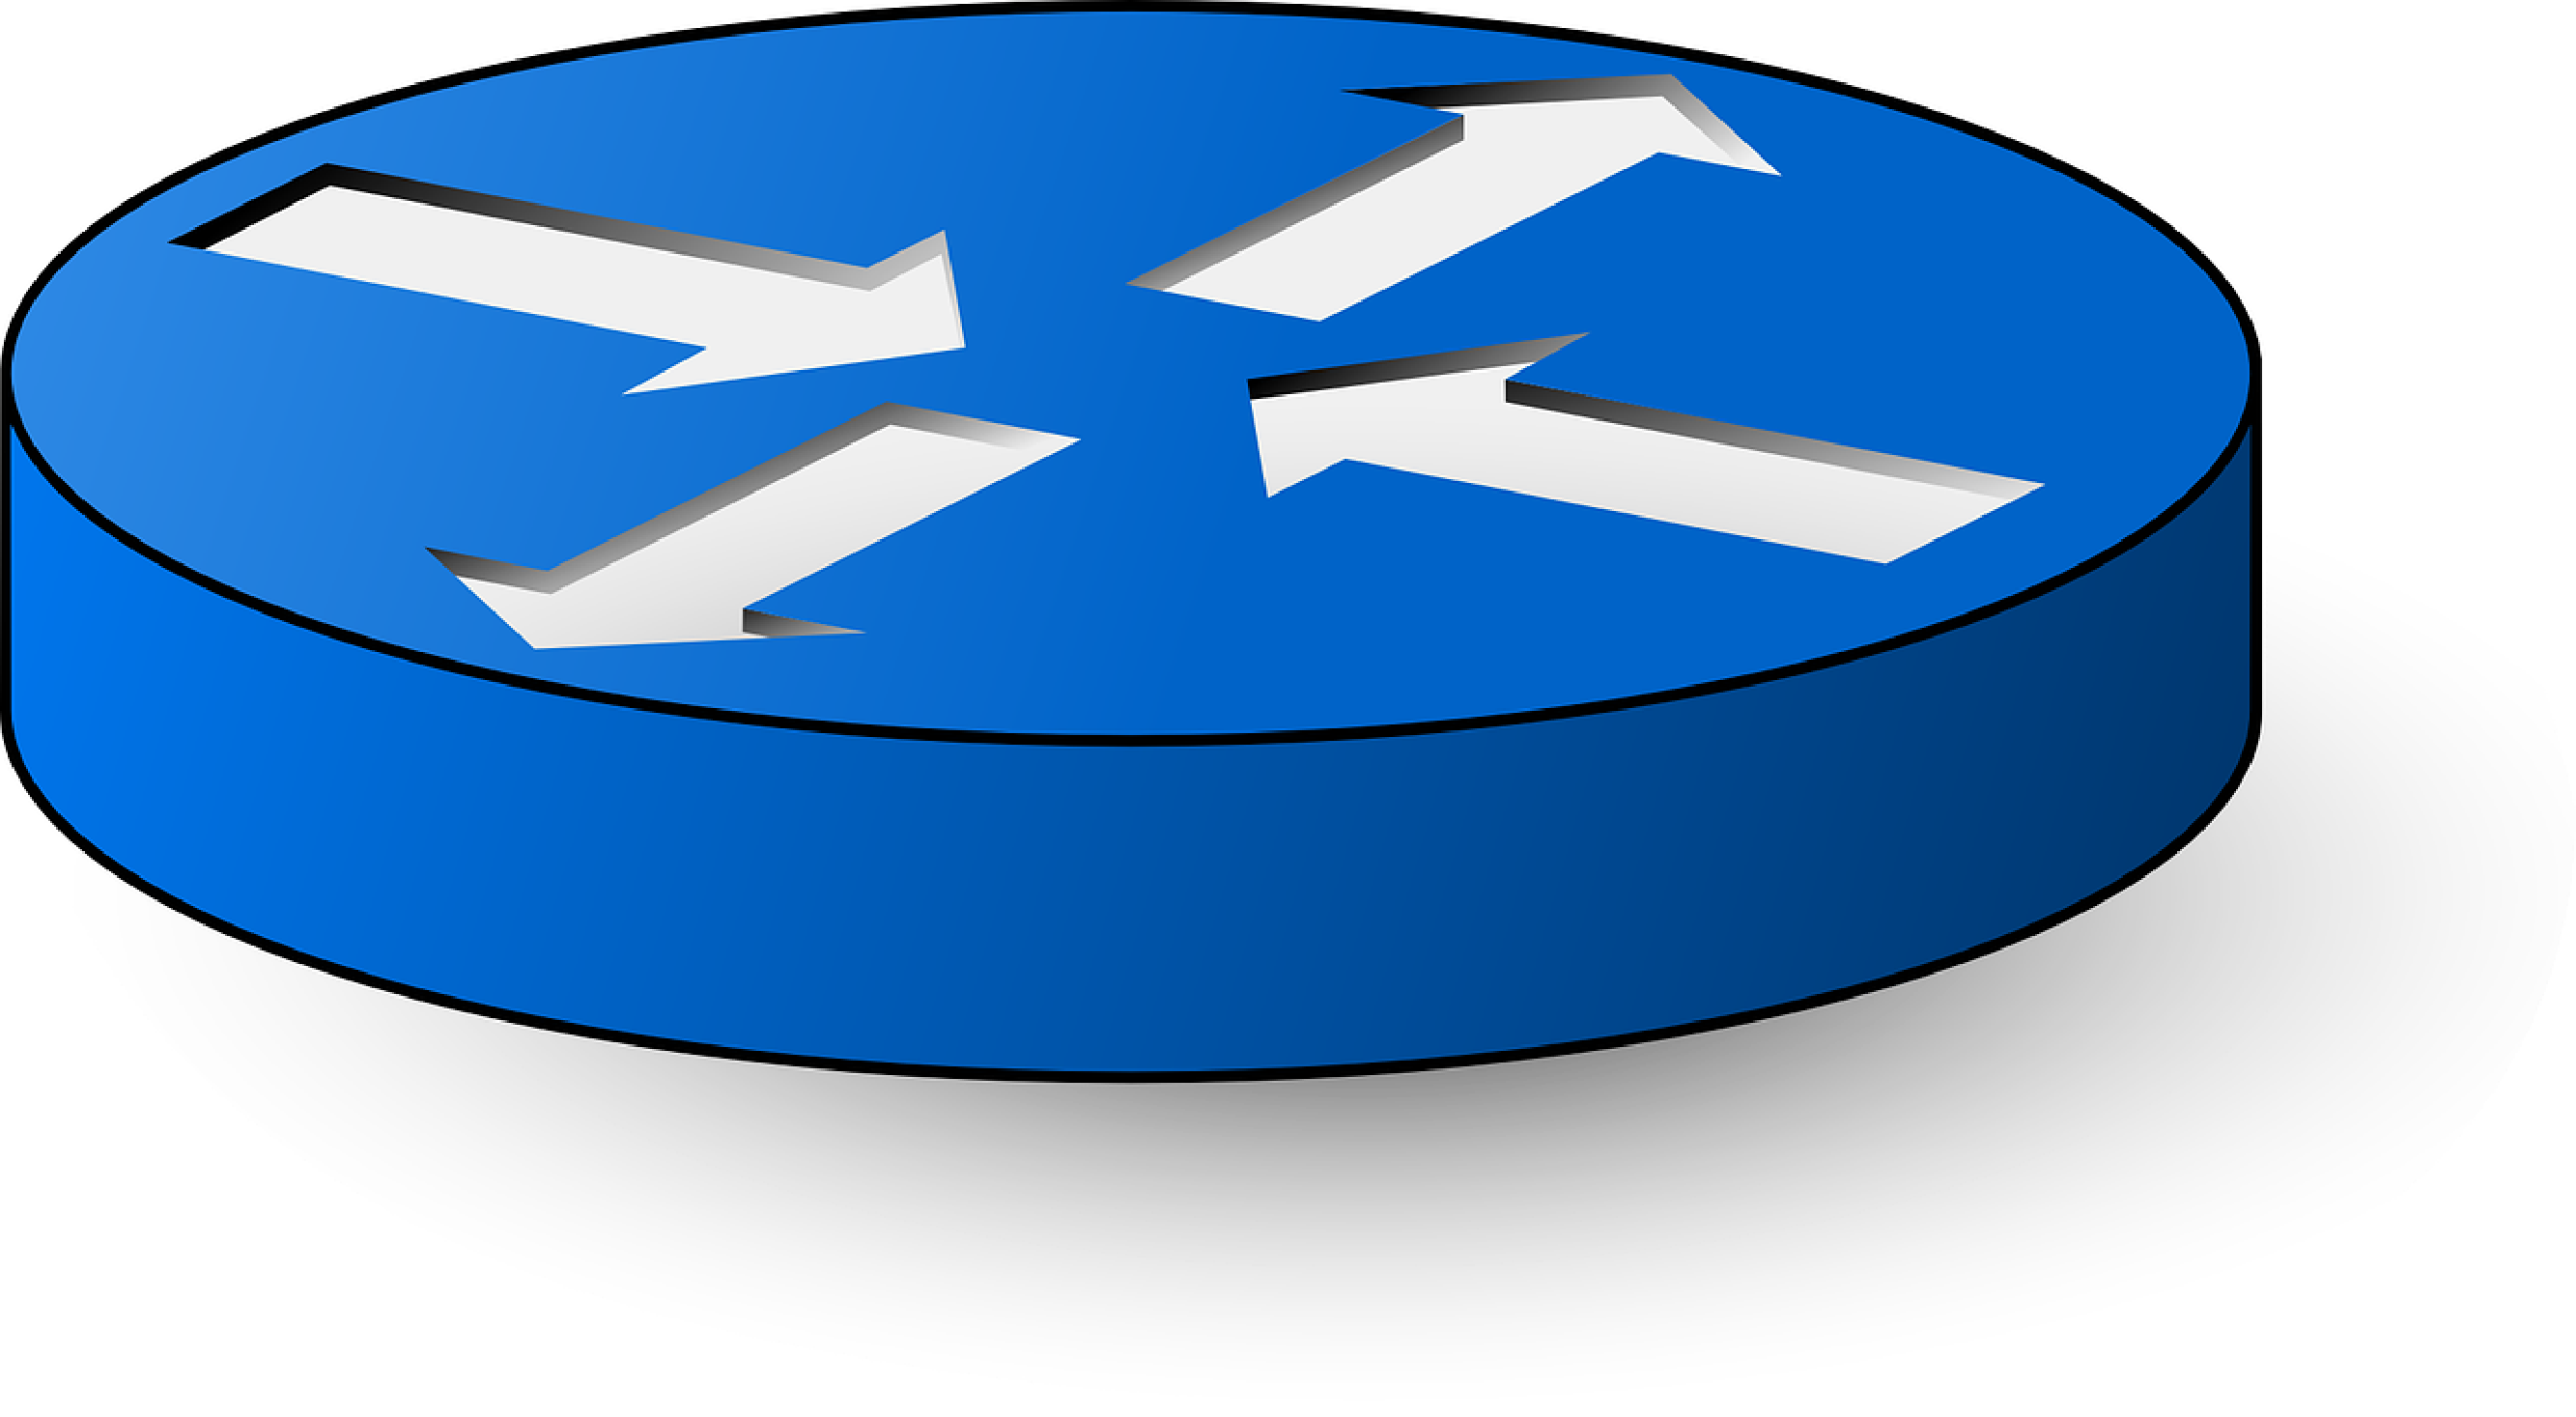
\includegraphics[width=52.5pt,height=52.5pt]{figures/router-30140_1280.pdf}};
%Image [id:dp9442712298825287] 
\draw (440.5,444.5) node  {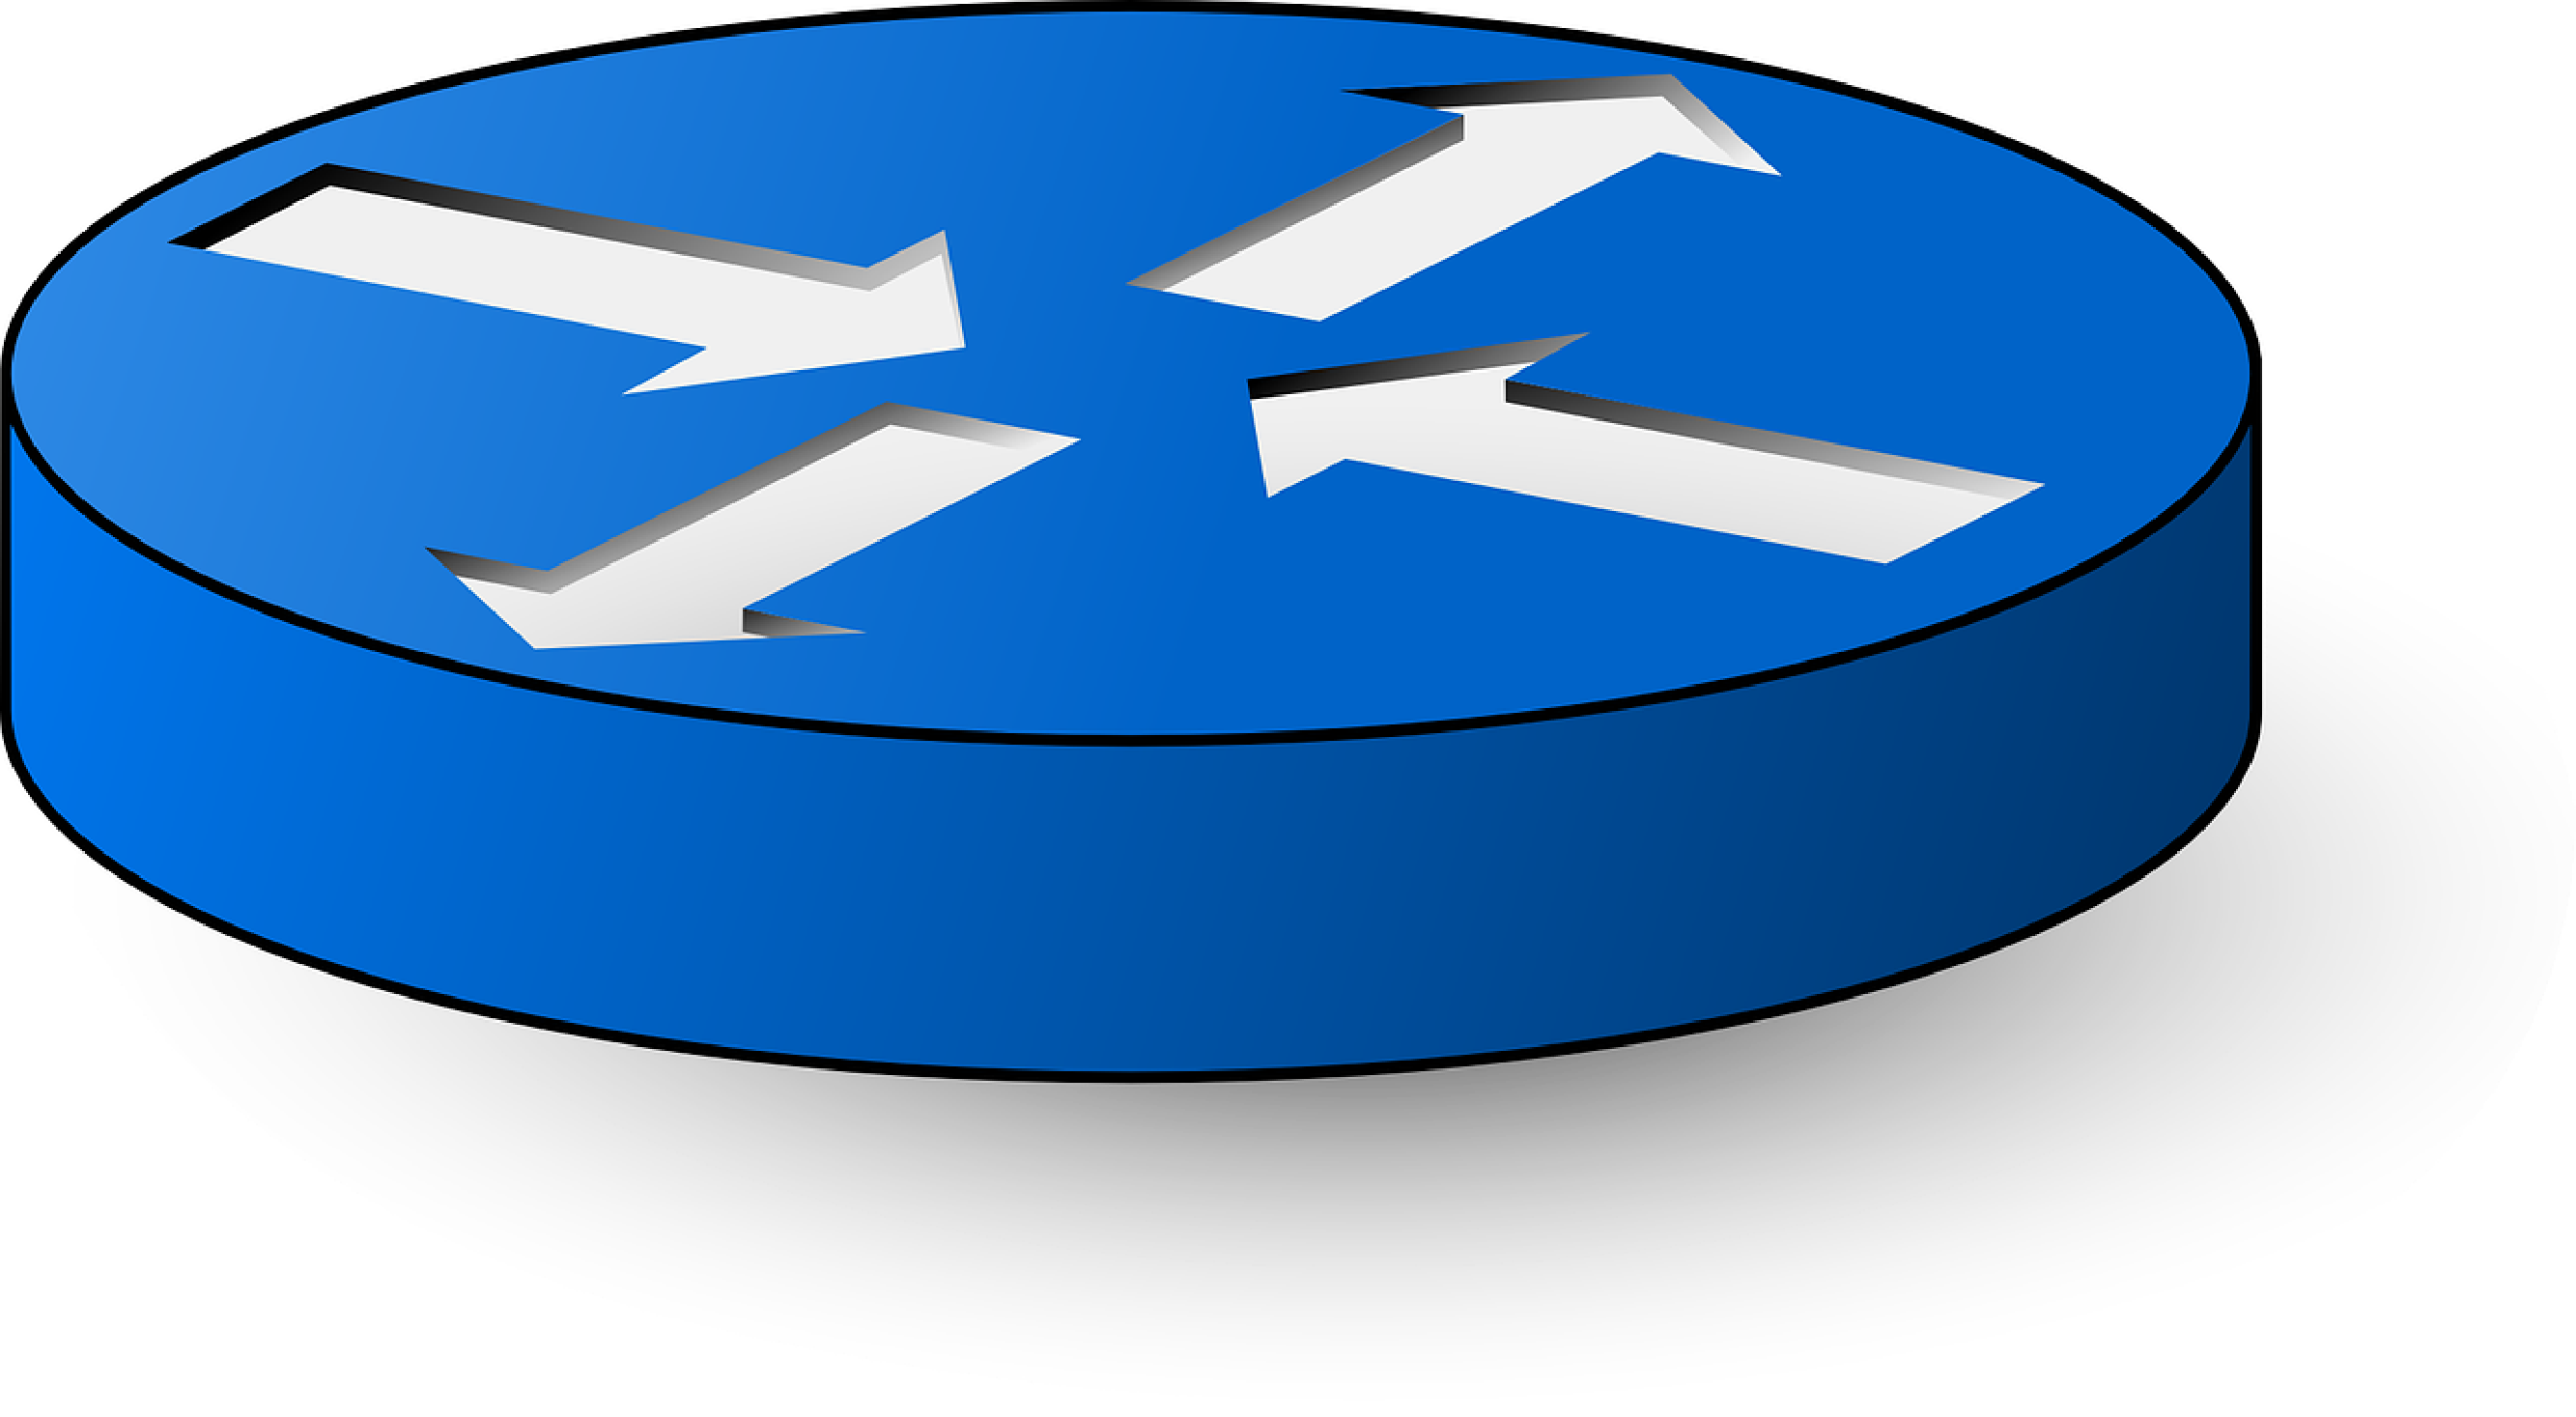
\includegraphics[width=52.5pt,height=52.5pt]{figures/router-30140_1280.pdf}};
%Straight Lines [id:da09222939335266478] 
\draw [color={rgb, 255:red, 74; green, 144; blue, 226 }  ,draw opacity=1 ][line width=1.5]    (236,313.33) -- (66.35,447.31) ;
\draw [shift={(64,449.17)}, rotate = 321.7] [color={rgb, 255:red, 74; green, 144; blue, 226 }  ,draw opacity=1 ][line width=1.5]    (14.21,-4.28) .. controls (9.04,-1.82) and (4.3,-0.39) .. (0,0) .. controls (4.3,0.39) and (9.04,1.82) .. (14.21,4.28)   ;

%Straight Lines [id:da6866328735169647] 
\draw [color={rgb, 255:red, 74; green, 144; blue, 226 }  ,draw opacity=1 ][line width=1.5]    (236,313.33) -- (432.28,405.56) ;
\draw [shift={(435,406.83)}, rotate = 205.17000000000002] [color={rgb, 255:red, 74; green, 144; blue, 226 }  ,draw opacity=1 ][line width=1.5]    (14.21,-4.28) .. controls (9.04,-1.82) and (4.3,-0.39) .. (0,0) .. controls (4.3,0.39) and (9.04,1.82) .. (14.21,4.28)   ;

%Shape: Cloud [id:dp2992812680460014] 
\draw  [fill={rgb, 255:red, 255; green, 255; blue, 255 }  ,fill opacity=1 ] (557.19,464.58) .. controls (556.29,457.33) and (559.25,450.16) .. (564.82,446.11) .. controls (570.39,442.05) and (577.58,441.82) .. (583.36,445.52) .. controls (585.4,441.31) and (589.14,438.4) .. (593.45,437.68) .. controls (597.76,436.95) and (602.13,438.5) .. (605.24,441.84) .. controls (606.98,438.02) and (610.4,435.46) .. (614.28,435.06) .. controls (618.17,434.65) and (621.97,436.47) .. (624.34,439.87) .. controls (627.48,435.82) and (632.49,434.11) .. (637.19,435.49) .. controls (641.89,436.87) and (645.44,441.08) .. (646.31,446.3) .. controls (650.16,447.45) and (653.38,450.37) .. (655.11,454.31) .. controls (656.85,458.25) and (656.94,462.82) .. (655.37,466.84) .. controls (659.17,472.24) and (660.06,479.44) .. (657.7,485.75) .. controls (655.35,492.05) and (650.11,496.52) .. (643.94,497.49) .. controls (643.9,503.41) and (640.93,508.84) .. (636.17,511.69) .. controls (631.42,514.54) and (625.63,514.36) .. (621.03,511.23) .. controls (619.07,518.32) and (613.56,523.53) .. (606.87,524.62) .. controls (600.18,525.71) and (593.52,522.48) .. (589.76,516.32) .. controls (585.16,519.36) and (579.63,520.23) .. (574.43,518.75) .. controls (569.23,517.27) and (564.8,513.55) .. (562.12,508.44) .. controls (557.42,509.04) and (552.87,506.37) .. (550.73,501.76) .. controls (548.6,497.16) and (549.33,491.58) .. (552.57,487.81) .. controls (548.37,485.11) and (546.23,479.75) .. (547.26,474.53) .. controls (548.29,469.31) and (552.26,465.41) .. (557.1,464.86) ; \draw   (552.57,487.81) .. controls (554.55,489.09) and (556.84,489.67) .. (559.13,489.47)(562.12,508.44) .. controls (563.11,508.31) and (564.07,508.04) .. (564.99,507.64)(589.76,516.32) .. controls (589.07,515.19) and (588.49,513.97) .. (588.04,512.7)(621.03,511.23) .. controls (621.39,509.94) and (621.62,508.6) .. (621.72,507.26)(643.94,497.49) .. controls (643.99,491.19) and (640.71,485.42) .. (635.52,482.66)(655.37,466.84) .. controls (654.53,468.99) and (653.24,470.89) .. (651.62,472.4)(646.31,446.3) .. controls (646.45,447.16) and (646.52,448.04) .. (646.5,448.93)(624.34,439.87) .. controls (623.55,440.87) and (622.91,442) .. (622.42,443.21)(605.24,441.84) .. controls (604.82,442.76) and (604.51,443.73) .. (604.31,444.73)(583.36,445.52) .. controls (584.58,446.3) and (585.71,447.24) .. (586.72,448.32)(557.19,464.58) .. controls (557.32,465.58) and (557.51,466.56) .. (557.78,467.53) ;
%Straight Lines [id:da885478252254038] 
\draw [line width=1.5]  [dash pattern={on 1.69pt off 2.76pt}]  (435.5,26.33) -- (474.5,26.83) ;


%Straight Lines [id:da6105591508346683] 
\draw    (435,42.71) -- (475,43.21) ;


%Straight Lines [id:da021279170004724568] 
\draw [color={rgb, 255:red, 74; green, 144; blue, 226 }  ,draw opacity=1 ][line width=1.5]    (438.5,75.13) -- (468.5,74.97) ;
\draw [shift={(471.5,74.96)}, rotate = 539.71] [color={rgb, 255:red, 74; green, 144; blue, 226 }  ,draw opacity=1 ][line width=1.5]    (14.21,-4.28) .. controls (9.04,-1.82) and (4.3,-0.39) .. (0,0) .. controls (4.3,0.39) and (9.04,1.82) .. (14.21,4.28)   ;

%Rounded Rect [id:dp201331626843132] 
\draw  [fill={rgb, 255:red, 217; green, 154; blue, 232 }  ,fill opacity=1 ] (6,276.78) .. controls (6,271.88) and (9.98,267.9) .. (14.89,267.9) -- (500.11,267.9) .. controls (505.02,267.9) and (509,271.88) .. (509,276.78) -- (509,303.45) .. controls (509,308.35) and (505.02,312.33) .. (500.11,312.33) -- (14.89,312.33) .. controls (9.98,312.33) and (6,308.35) .. (6,303.45) -- cycle ;

%Shape: Polygon Curved [id:ds08242749430225138] 
\draw  [color={rgb, 255:red, 255; green, 248; blue, 177 }  ,draw opacity=1 ][line width=2.25]  (41,423.33) .. controls (61,413.33) and (210,392.33) .. (232,407.33) .. controls (254,422.33) and (264,544.33) .. (248,574.33) .. controls (232,604.33) and (53.5,538.83) .. (33.5,508.83) .. controls (13.5,478.83) and (21,433.33) .. (41,423.33) -- cycle ;
%Straight Lines [id:da08659205633415445] 
\draw [color={rgb, 255:red, 255; green, 255; blue, 139 }  ,draw opacity=1 ][line width=2.25]    (435,91.71) -- (475,92.21) ;


%Straight Lines [id:da012161855616681594] 
\draw [color={rgb, 255:red, 242; green, 175; blue, 175 }  ,draw opacity=1 ][line width=2.25]    (435,111.71) -- (475,112.21) ;



% Text Node
\draw (55,213) node  [align=left] {(A1)};
% Text Node
\draw (211,471) node  [align=left] {(A3)};
% Text Node
\draw (113,594) node  [align=left] {Physical Infrastructure};
% Text Node
\draw (599,474) node  [align=left] {Internet};
% Text Node
\draw (417,171) node  [align=left] {(A2)};
% Text Node
\draw (587,501) node  [align=left] {(A4)};
% Text Node
\draw (521,26) node  [align=left] {Virtual Link};
% Text Node
\draw (528,47) node  [align=left] {Physical Link};
% Text Node
\draw (562,69) node  [align=left] {Hypervisor - Switch link};
% Text Node
\draw (548,92) node  [align=left] {vSDN1 Embedding};
% Text Node
\draw (549,113) node  [align=left] {vSDN2 Embedding};
% Text Node
\draw (257.5,290.11) node  [align=left] {Network Hypervisor};
% Text Node
\draw (55.76,67.79) node  [align=left] {{\small vSDN1}};
% Text Node
\draw (282.98,171.5) node [scale=0.9] [align=left] {{\small vSDN2}};


\end{tikzpicture}

\caption{Attack surface of the SDN environment}
\label{fig:attack-surface}
\end{figure}

%\GB{I suggest: ``Attacks against Migration'' as a title}
\label{sec:attacker-model}
The migration of a VN creates virtual nodes and virtual links between them.
Thus, based on  the migration functions we introduced in Section~\ref{sec:migration} and the axioms we have presented in Section~\ref{sec:prop-conf}, we will describe the different components of a threat using the following syntax
%\GB{terms?}
%\FC{The syntax is the combination of terms}
: Attacker - Action - Target.

\subsubsection{Attacker}
We consider the different locations from where an attacker could attack the migration of the VN. 
Figure~\ref{fig:attack-surface} places four different attackers: the insider (A1), the collocated user (A2), the provider (A3), the outsider (A4).

The insider is an attacker located inside the VN that is going to be migrated.
It can be a malicious user able to control a virtual node and deploy incorrect flow rules.
The collocated user is another user of the virtualization platform.
He can use his own topology on the physical infrastructure.
The provider is the owner of the physical infrastructure.
He has access to the SDN switches embedding the virtual topologies.
The outsider is a malicious user outside the SDN environment.
He has limited access to both the VNs and the physical infrastructure.

\subsubsection{Action}
There are 4 major actions that can be performed by an attacker to affect the VNs and their environment.
The first two are related to the infrastructure and the others are related to the data carried across the network.
\begin{itemize}
\item Unauthorized access to a network element.
\\ This type of access represent a violation of each security property.
\item Disruption of service on a network element.
\\ The availability of physical and virtual resources becomes compromised
\item Information disclosure without authorization.
\\ The confidentiality of the data is affected
\item Information modification or destruction without authorization.
\\ The integrity of the data or the network resource is affected
\end{itemize}

\subsubsection{Target}
We can consider two types of targets: nodes or data.
The nodes are either the physical switches in the infrastructure or the virtual nodes of a VN.
There are three types of data inside a VN and its infrastructure.
The user data carried by the virtual elements, the management data and the configuration data carried by the infrastructure. 

The user data is the traffic generated by the user and going through the VN.
The management data is made of the different packets exchanged between the virtualization layer and the physical infrastructure to operate properly (capacities, established links, etc.).
The configuration data are the different flow rules deployed on the physical switches when instantiating a VN.
It is important to note that both configuration data and management data are issued by the hypervisor but do not serve the same purpose nor have the same frequency of use, even though they use the same communication channel.
Management data are regularly exchanged between the hypervisor and the switch to maintain the view of the infrastructure (\eg symmetric messages like HELLO requests), while configuration data are sent when installing new flow rules or removing old ones (asynchronous messages sent because of flow expiration).

\begin{table}[h]
\centering
\begin{tabular}{|l|l|l|}
\hline
\textbf{Attacker}   & \textbf{Action}    & \textbf{Target}             \\ \hline
Insider    & Unauthorized access                  & Nodes              \\ \hline
Collocated & Disruption of service                & User data          \\ \hline
Provider   & Information disclosure               & Management data    \\ \hline
Outsider   & Information modification/destruction & Configuration data \\ \hline
\end{tabular}
\caption{Elements of the attack model}
\label{tab:attack-model}
\end{table}

\subsubsection{Attacks}
\label{sec:model-attacks}
%\GB{please in this section and the following, specify which attack is directed against which algorithm}
In the previous sections, we have defined the different attackers, as well as the malevolent actions and possible targets in the virtualization infrastructure. 
Table~\ref{tab:attack-model} summarizes these information.
We will combine elements from each column together to define several attacks targeting the migration process or the user's data.
These attacks are based on two assumptions: a stable initial environment and no outsider attacker.
We consider that the virtualization infrastructure is not already under attack when a malicious user decides to launch one of the following attacks.
This assumption comes from the fact that we aim to detect the switch between a safe state and a compromised state. From a practical point of view, the infrastructure runs most of the time with a normal behavior.
We also assume that an attacker residing outside the virtualization infrastructure and not using the virtualization service has little to no attack surface on the infrastructure.
Most interfaces to interact with any component of the system are limited in visibility from the outside world.
For instance, the DPAC provides an interface for end users to interact with their virtual network, and there is no openly identified weaknesses for an outsider to use (\ie the hypervisor will reject commands from unauthorized users).
Similarly, the CPAC provides an interface between the hypervisor and the physical nodes, and there is no functional use for this component to be interfaced with the outside world.
We summarize the attacks in Table~\ref{tab:use-case-attack}.

% Please add the following required packages to your document preamble:
% \usepackage{graphicx}
\begin{table}[h]
\resizebox{\textwidth}{!}{%
\begin{tabular}{|l|l|l|l|l|}
\hline
Attack                   & Attacker        & Action                      & Target                   & Summary                                                                  \\ \hline
Denial of Service        & Provider side   & Service disruption          & Nodes                    & Resource depletion (DNS amplification ICMP flood) \\ \hline
Info. Disclosure   & Collocated user & Info. disclosure   & Node, user data          & Data exfiltration by malicious flow rules injection    \\ \hline
Config. alteration & Provider side   & Info. modification & Node, config. data & Man-in-the-middle attack to Modify config. data             \\ \hline
Denial of Service        & Provider side   & Service disruption          & Nodes                    & Resource depletion (DNS amplification ICMP flood) \\ \hline
\end{tabular}%
}
\caption{Use cases: Attacking the migration}
\label{tab:use-case-attack}
\end{table}
% In this paper, we chose to focus on the security aspects of the confidentiality.
% Thus, we are more interested in the unauthorized access and information disclosure of the attack model.
% As we also consider a stable initial environment, an outsider attacker is too limited to attack the infrastructure and is therefore of no interest in this paper.
% Finally, the different data present in the threat model are similar enough in essence.
% Attacking one or another makes no difference in terms of formal modeling.
% We propose two different attacks, one focusing on the disclosure of confidential traffic carried by a VN, and the other will be an on-site attack on a physical node.
%\GB{please specify which migration algorithms are attacked here, and in the next section}

%\GB{in general, you could sum up in a table what attacker can do what against what. I am surprised that you only have two scenarios. Usually attacker classes tend to be ordered sets. But it is not always the case}
%\FC{I believe one attack scenario per migration algorithm is enough. However I agree with the table, will work on it today. I don't understand what you mean by ordered sets.}
%\GB{usually, you describe different attackers that share abilities, from the least potent to the most potent. Usually the least potent has ability to perform action A, then the second least potent can do actions A and B, then another can do actions A, C and D, and the most potent can do A, B, C and D. If you are presenting only a couple of scenarios, you may actually list all possible scenarios, \ie triplets (Attacker, Action, Target) and explicitly state that you will only demonstrate two of them, motivating why you choose these}




\paragraph{Denial of Service}\textbf{\\}
In this scenario, the attacker is located inside the physical infrastructure, and will launch Denial of Service (DoS) attacks to render one or several nodes unavailable.
This will result in a forced migration, thus creating an opportunity to compromise the migration process.
This attack becomes the necessary first step of all of the following attacks.

\subparagraph{Hypotheses}\textbf{\\}
% \textbf{Location:} The attacker is located either inside the physical infrastructure or is a malicious user of the virtualization service.\\
\textbf{Information gathering}\textbf{\\}
THe attacker has collected information about his victim, and how to precisely target network equipments.
The information collection process is considered out of scope of this work.\\
\textbf{Traffic generation:} The attacker can generate enough traffic to cause a service disruption.
DoS attacks like ICMP flood or DNS amplification are used for to deplete network resources in the infrastructure.

\subparagraph{Attack methodology}\textbf{\\}
The attacker will generate massive amounts of traffic to generate congestion effects inside the network. The attacker may be located inside the physical network, or he may be the owner of a Virtual Network. The second option is easier to achieve but the attacker will be confronted to the resource isolation enforced by the hypervisor (\ie FlowVisor bandwidth isolation mechanism)


\subparagraph{Impacts}\textbf{\\}
This attack impacts the following security properties:\\
The \textbf{availability} of nodes in the infrastructure has been impacted because of the DoS attack.
% \begin{itemize}
%     \item $node\_availability(N)$
%     \item $vnode\_availability(n)$
%     \item $vlink\_availability(l)$
%     \item $path\_availability(P)$
%     \item $vpath\_availability(P)$
% \end{itemize}

\paragraph{Information disclosure}\textbf{\\}
In this scenario, the attacker is a collocated user that is gaining access to another user's confidential traffic. 
\subparagraph{Hypotheses:}\textbf{\\}
\textbf{Collocated attacker:} The attacker owns a virtual network in the infrastructure.\\
\textbf{Migration trigger:} The attacker can trigger the migration of the victim's VN.\\
\textbf{Embedding knowledge:} The attacker has approximate knowledge of the new substrate network.\\
\textbf{Writing rights:} The attacker can install specific flow rules inside a node.

\subparagraph{Attack methodology:}\textbf{\\}
In order to gain access to confidential data, the attacker generates instability in the infrastructure. Typically, generating lots of requests between nodes and users will create enough disruption to force the migration.
Then, he will use his knowledge of the embedding of the virtual network to target specific nodes.
Deploying probes in the network or attacking on a large scale the infrastructure could lead the virtualization layer to a particular deployment. Co-residency-based attacks and vulnerabilities are exploited in several cases~\cite{malicious-atya2017,nomad-Moon2015b,getoffmucloud-Ristenpart2009,stalling-atya2017}.
An attacker uses time-based attacks to verify the co-residency with his victim and then the attacker will compromise the confidential data by redirecting it from the victim's VN toward a malicious end host belonging to him.
Such attacks rely on deploying specific flow rules on a set of physical nodes that will copy the confidential traffic and route it towards the attacker.
This methodology is illustrated in~\cite{Costa2015,Sphinx-Dhawan2015}.


\subparagraph{Impacts}\textbf{\\}
This attack impacts the following security properties:\\
The \textbf{availability} of specific nodes in the infrastructure has been impacted to force the migration.
% \begin{itemize}
%     \item $node\_availability(N)$
%     \item $vnode\_availability(n)$
%     \item $vlink\_availability(l)$
%     \item $path\_availability(P)$
%     \item $vpath\_availability(P)$
% \end{itemize}
The \textbf{confidentiality} of the data that has been extracted by the attacker.
% \begin{itemize}
%     \item $confidentiality(D)$
% \end{itemize}
The confidentiality of the nodes is not impacted because the attacker did not access the node by installing flow rules on them, with respect to the definition provided in the previous section.\\
The \textbf{integrity} of the different nodes that have been used to forward the data to the attacker.
%     \begin{itemize}
%     \item $node\_integrity(N)$
%     \item $vnode\_integrity(n)$
%     \item $vlink\_integrity(l)$
% \end{itemize}
The \textbf{co-residency} between both victim and attacker VNs has been increased for the attacker to successfully exfiltrate the victim's data.


\paragraph{Migration alteration}\textbf{\\}
We now consider a malicious user intending to exploit the migration process to modify the configuration deployed on a node.

\subparagraph{Hypotheses:}\textbf{\\}
\textbf{Provider side attacker:} The attacker sits between the node and the hypervisor.\\
\textbf{Man-in-the-middle:} The attacker can modify the configuration information sent by the hypervisor in a specific node.\\
\textbf{Migration trigger:} The attacker can trigger the migration of the victim's VN.\\
\textbf{Embedding knowledge:} The attacker has approximate knowledge of the new substrate network.

\subparagraph{Attack methodology:}\textbf{\\}
First of all, the attacker gains access to a networking equipment between the target node and the hypervisor. Similarly to the previous attack, this is done by exploiting vulnerabilities in the physical equipments.
Then, he will trigger the migration of a specific physical node, that will be redeployed on the node targeted by the Man-in-the-middle attack.
Once the hypervisor sends the different flow rules, the attacker will modify them to fit his extraction scheme.

\subparagraph{Impacts:}\textbf{\\}
This attack impacts the following security properties:\\
The \textbf{availability} of the attacked node has been impacted to trigger the migration.
% \begin{itemize}
%     \item $node\_availability(N)$
%     \item $vnode\_availability(n)$
%     \item $vlink\_availability(l)$
%     \item $path\_availability(P)$
%     \item $vpath\_availability(P)$
% \end{itemize}
The \textbf{confidentiality} of the configuration data that has been modified by the attacker.
% \begin{itemize}
%     \item $config\_confidentiality(conf)$
% \end{itemize}
The confidentiality of the nodes is not impacted for the same reasons described in the previous attack.\\
The \textbf{integrity} of the node and its configuration has been compromised
%     \begin{itemize}
%     \item $node\_integrity(N)$
%     \item $vnode\_integrity(n)$
%     \item $vlink\_integrity(l)$
%     \item $config\_integrity(conf)$
% \end{itemize}

% 


\subsection{Problem verification using a theorem prover}
The formal model and the different attacks we have described in the previous sections allow us to represent the security of the migration of virtual network. The security is defined in terms of predicates and equations, and can be evaluated using a theorem prover.
In this section, we detail theoretical aspects of theorem proving, then, we will present the theorem prover used in our work, SNARK~\cite{snark-Stickel2000}.

\subsubsection{Formal theory about theorem proving}
\label{sec:proving-theory}
We present in this section specific aspects of first order logic theorem proving that will be used later on in this thesis. We will give a brief overview of the first order logic theory and we will then present the basics of theorem proving and several verification mechanisms.

\paragraph{First order logic}
The first order logic is a formal system describing a theory using declarative propositions, predicates and quantification.

A declarative proposition, also referred to as a clause, is a set of terms  that may be connected together using logical operators.
We illustrate this with the following example:

$P \Rightarrow Q$ means "$P$ implies $Q$``. $P$ and $Q$ are the terms of the clause and $\Rightarrow$ is the logical operator representing implication.

The first order logic admits the following logical operators:

\begin{itemize}
    \item $\forall$: The forall operator, $\forall x\in S$ means for all elements $x$ in set $S$.
    \item $\exists$: The exist operator, $\exists x\in S$ means there exist at least one $x$ in set $S$.
    \item $\neg$: The negation operator, $\neg A$ means then logical negation of A, often noted $\overline{A}$.
    \item $\wedge$: The conjunction operator, $A \wedge B$ means the logical arithmetic A AND B.
    \item $\vee$: The disjunction operator, $A \vee B$ means the logical arithmetic A OR B.
    \item brackets $( )$: Brackets are used to order the resolution of the logical proposition, similarly to traditional arithmetic.
    \item $\Rightarrow$: The implication operator, $A \Rightarrow B$ means A implies B.
    \item $\Leftrightarrow$: The bidirectional implication operator, $A \Leftrightarrow B$ means "A implies B`` AND "B implies A``.
\end{itemize}

Predicates are functions taking a set of terms (variables) as input and returning a binary value, True or False, as an output.

For instance, we can define $P(A,B,C) = A \wedge (B \vee C)$, which would yield for the following example: $P(True,False,True)=True$.

\paragraph{First order logic Theorem Proving}\textbf{\\}
The purpose of theorem proving is to determine if a set of clauses is satisfiable or unsatisfiable.
A satisfiable clause that admits a solution that makes it true.
An unsatisfiable clause is a clause that cannot be true no matter the values of its terms.
The theorem prover will apply inference rules on the original set of clauses and try to reach another set of clauses where the satisfiability can be determined.

We will now present some rules of inference used for first order logic theorem proving.
A rule of inference is a rule defining the deduction process, it takes a set of propositions as input and returns a proposition which is a conclusion drawn from the input propositions.

We use $\vdash$ to represent the result of the deduction from a set of proposition.

\paragraph{Modus ponens and modus tollens}\textbf{\\}
Modus ponens is a rule of inference using the affirmation in an implication to deduce the conclusion.
Considering the simple example given previously, $P \Rightarrow Q$, if we assert that $P$ is true, then we use modus ponens to conclude that $Q$ is true as well. This is summarized as "If P implies Q and P is true, then Q must be true" : $P \Rightarrow Q, P \vdash Q$.

Similarly Modus tollens uses the negation in the consequence of an implication to deduce the conclusion.
Considering $P \Rightarrow Q$, asserting that $Q$ if false, then $P$ must be false as well: $P \Rightarrow Q, \neg Q \vdash \neg P$.

\paragraph{Resolution principle}\textbf{\\}
The resolution principle, shortened to resolution, is an inference rule satisfying the completeness property. Completeness implies that applying the resolution to an unsatisfiable clause will always yield false. 

For instance, $P \wedge \neg P$ is obviously unsatisfiable, \ie it is always False.

The resolution principle uses substitution in a set of clauses to reach a conclusion.
We consider the simple example presented in~\cite{snark-Stickel2000} and refer the reader to~\cite{symbolic-proof} for additional reading, more specifically on variable unification.
We also refer the reader to the Method of Davis and Putnam and more specifically on the One-Literal Rule.

Consider the following clauses: $\neg P \vee Q$ and $P \vee R$. The resolution principle returns $Q \vee R$ as a resolvent of the previous propositions.


\paragraph{Paramodulation}\textbf{\\}
The paramodulation is an inference rule used to exploit the equality existing between terms and the occurrence of term in a proposition. The paramodulation can be seen as \textit{substitution in case of equality}.

Consider the proposition $P(x) = true$ and the quality $x=y$. Therefore, we can infer that $P(y)$ will also yield True.

Consider now the two propositions: $P(x) \vee Q(y)$, $(x = y) \vee R(y)$, paramodulation deduces the proposition $P(y) \vee Q(y) \vee R(y)$.\\
$P(x) \vee Q(y)$, $(x = y) \vee R(y) \vdash P(y) \vee Q(y) \vee R(y)$

\paragraph{Rewriting rules}\textbf{\\}
Rewriting rules are used to replace an expression by another in a set of propositions.
This is done to simplify the search space when applying inference rules~\cite{snark-Stickel2000}.

We illustrate this with a simple example: $P \Leftrightarrow Q \wedge R, P \vee T$ is rewritten as $Q \wedge R \vee T$. 

The rewriting rule may be condition to replace the left hand side of an equivalence by the other, but may also apply substitutions to terms in the proposition only on one side of the proposition.
We also refer the reader to~\cite{snark-Stickel2000,symbolic-proof} for further explanations.





\subsubsection{SNARK: A first order temporal logic theorem prover}
\label{sec:proof-detects-violation}
%Part of this effort is devoted to using automatic reasoning to establish that a network enforces confidentiality properties or to detect that such properties can be violated.
In section~\ref{sec:proving-theory}, we have described several aspects of the first order logic theorem proving theory.
In this section we  present a first-order theorem prover that will be used to detect the violation of the security properties.
We use the Stanford Research Institute's open-source first-order reasoner SNARK~\cite{snark-Stickel2000}.

SNARK is fully automatic and uses machine-oriented inference rules, such as \textit{resolution} for general-purpose reasoning and \textit{paramodulation} and \textit{rewriting} for reasoning about equality.
It has special facilities
%\GB{is listing all features supported by SNARK relevant in the paper?} 
for accelerated reasoning about space and time; a sort mechanism for internalizing the reasoning about sorts or types; and an \textit{answer extraction} mechanism for constructing an answer to a query from a completed proof. 
Although SNARK is ideally suited for our purpose and has been successfully used in other applications (\eg~\cite{AICPub2006:2015}), any other theorem prover with comparable features could be used.

SNARK is a refutation procedure, \ie it looks for inconsistencies in a set of logical sentences. It begins with a theory, a set of axioms, \ie logical sentences that specify the basic properties of the subject domain. 
When trying to prove that a conjecture holds in the theory, it negates the conjecture, adds it to the set of axioms of the theory, and tries to find a contradiction in the resulting set. 
For this purpose, it will apply inference rules, which deduce new sentences, and adds those to the set. The process continues until no further inferences are possible or until a contradiction is obtained \-—-- this shows that the negated conjecture is inconsistent with the axioms of the theory and, hence, that the conjecture itself is valid in the theory. 
Once the conjecture is proven, it is regarded as a theorem of the theory; before that, its validity is in question.
The answer extraction mechanism, developed for program synthesis applications~\cite{Manna:1980:DAP:357084.357090}, associates with each sentence in the set an answer term, such that if the sentence can be falsified, the corresponding instance of the answer term will satisfy the original query. 
When a contradiction is obtained, any instance of the contradictory sentence is false, and hence the corresponding answer term will always  be an answer to the query. 
Typically, there are many proofs of a given theorem, each leading to a possibly different answer. 
These can be assembled and presented to the user.

The order in which inference rules are applied depends on a set of heuristic principles which are under the control of the developer of the theory. 
Weights can be assigned to symbols, which cause SNARK to focus attention on “lighter” sentences in its set. 
Also, an ordering is applied to symbols, which cause SNARK to focus on particular parts of a sentence. 
Typically, symbols will be replaced by other symbols that are smaller in the ordering. 
Since first-order theorem proving is undecidable and the search can go on forever, we give SNARK a time limit on proving a given theorem. 
This is set empirically \-—-- for the examples considered here, most of the theorems were proven in less than a second. The bigger use cases presented later took no more than 30 seconds.
SNARK will automatically search for a series of proofs of a given conjecture, each yielding a different answer.
In general, there may be an infinity of answers to a query, but we rely on the time limit mechanism to cut off the search.

%\GB{most of the contents before describe how SNARK works in rather technical terms. Although interesting, it may be out of the scope of the paper to explain in such details how SNARK works. It should be summarized to highlight what are tehe most important features of SNARK formalizing and solving our migration problem. To that end, the illupstrative example below is what is expected from this paper}

\subsubsection{Proving a simple violation with SNARK}
\label{sec:find-violation}
The operation and formalism of SNARK will be illustrated in the context of a simple example.
We are given an axiomatic theory of the domain of network confidentiality, and we use SNARK to detect a confidentiality violation during the migration of a virtual network.
This example makes a simple assumption regarding the possibility of reading a piece of data in the network. If the data is carried by a node during a certain time interval, then it can be read via the nodes connected to it, directly or via a path of nodes, during a subset of this time interval.
This assumption alleviate the unnecessary burden of modeling the actual routing performed by network nodes and will instead focus on the configuration installed in the nodes.
Rather than presenting the axioms of the theory in advance, we will introduce them as they are required in the proof.

Note that SNARK adopts a LISP-like notation for expressions; thus, we write \verb'(P A B)' rather than \verb'P(A, B)'. 
Variables with "\verb'?'" prefixes indicate entities that we must find as the proof is under way.
Variables in a sentence are ``dummies'' \---- they may be systematically renamed without changing the meaning of the sentence. 
The notation \verb'?t.t-int' is a variable \verb'?t' of type (sort) \verb't-int', \ie a time interval. 
Other variables are of sort \verb'user', \verb'data', and \verb'path'.
As the proof is under way, these variables will become instantiated with concrete terms of compatible sorts, \eg \verb'?u.user' with \verb'user-1'. 
These instantiations will be reflected in the corresponding answer term.

To find violations, we propose the \textit{data confidentiality violation conjecture}

\begin{lstlisting}[numbers=none] 
(exists (?u.user ?d.data ?p.path ?t.t-int)
  (data-confidentiality-violation 
     ?u.user ?d.data ?p.path 
     ?t.t-int))
     :answer '(ans ?u.user ?d.data ?p.path ?t.t-int)
\end{lstlisting}

In other words, we are establishing the existence of  a user, some data, a path of nodes, and a time interval that exhibits a violation of confidentiality. 
Once we find entities that exhibit the violation, they will compose the answer term that SNARK will extract from the proof:  
  \begin{lstlisting}[numbers=none] 
     (ans ?u.user ?d.data ?p.path ?t.t-int)
  \end{lstlisting}


A data confidentiality violation is defined in part by the following axiom:   
\begin{lstlisting}[]                                               
(implied-by
  (data-path-violation 
     ?u.user ?d.data ?p.path ?t.t-int)
  (and
    (= ?t.t-int
       (intersection
    	  (time-i ?r1.t-pt ?r2.t-pt)
    	  (time-i ?s1.t-pt ?s2.t-pt)))
    (reads-via-path
       ?u.user ?d.data ?p.path 
       (time-i ?r1.t-pt ?r2.t-pt))
    (not (is_authorized
       ?u.user ?d.data
       (time-i ?s1.t-pt ?s2.t-pt)))
    (non-empty ?t.t-int)))
\end{lstlisting}

In other words, the confidentiality violation can occur for a piece of data via a path of nodes during a time interval \verb'?t' if
%\GB{if all these conditions should hold together, I suggest to use the paraenum environment instead}
\begin{itemize}
\item the user can read the data via the path during a time interval \verb'?r' (lines 9-11)
\item the user is not authorized to read the data during a time interval \verb'?s' (lines 12-14)
\item the time interval \verb'?t' is the intersection of \verb'?r' and \verb'?s' (lines 6-8)
\item the time interval \verb'?t' is not empty (line 15)
\end{itemize}

Here  \verb't-pt' is the sort of time points, and \verb'(time-i ?t1.t-pt ?t2.t-pt)' is the time interval between the two time points \verb'?t1.t-pt' and \verb'?t2.t-pt'. If a user can read some data during one time interval and is not authorized to read that data during another time interval, a confidentiality violation can occur during the intersection of those two intervals, provided that the intersection is not empty.

Applying the resolution rule to the negated conjecture and the definition of a data confidentiality violation, and then simplifying, yields the following \textit{current proof step}, which is added to the set of consequences:

\begin{lstlisting}[] 
   (or 
    (not 
      (= ?t.t-int
         (time-i 
          (max-time ?r1.t-pt ?s1.t-pt)
          (min-time ?r2.t-pt ?s2.t-pt))))
    (not (reads-via-path
           ?u.user ?d.data ?p.path
           (time-i ?r1.t-pt ?r2.t-pt)))
    (is_authorized ?u.user ?d.data
       (time-i ?s1.t-pt ?s2.t-pt))
    (not (= ?t.t-int
            (time-i ?t1.t-pt ?t2.t-pt)))
    (not-before ?t1.t-pt ?t2.t-pt))
\end{lstlisting}
with associated answer term \verb' (ans ?u.user ?d.data ?p.path ?t.t-int)'.
This may be regarded as the negation of a goal to be established (line 2).
% ; conditions in the sentence are implicitly negated.
Thus, we are looking for a user who can read the data via a path of nodes but who is not authorized to do so (lines 7-11).
We establish that the intersection is not empty by showing that its endpoints are in temporal order, \ie the negation of \verb' (not-before ?t1.t-pt ?t2.t-pt)' (line 14).

Note that the intersection of the two intervals has been simplified to a single time-interval whose start point is the maximum of the two start-points and whose final point is the minimum of the two final points.  
This has been accomplished by rewriting the term according to an axiom of the theory:

\begin{lstlisting}[numbers=none]
 (= (intersection
          (time-i ?r1.t-pt ?r2.t-pt)
          (time-i ?s1.t-pt ?s2.t-pt))
       (time-i
          (max-time ?r1.t-pt ?s1.t-pt)
          (min-time ?r2.t-pt ?s2.t-pt)))
\end{lstlisting}


The relation \verb'reads-via-path' is defined in part by the axiom

\begin{lstlisting}
(implied-by
  (reads-via-path
    ?u.user ?d.data ?p.path ?t.t-int)
  (and
    (data-at-node 
       ?d.data ?n1.node 
       (time-i ?r1.t-pt ?r2.t-pt))
   (reads-at-node 
       ?u.user ?d.data ?n2.node 
       (time-i ?s1.t-pt ?s2.t-pt))
   (path-link 
       ?n1.node ?n2.node ?p.path 
       (time-i ?u1.t-pt ?u2.t-pt))   
    (= ?t.t-int
       (intersection
	     (time-i ?r1.t-pt ?r2.t-pt)
	     (intersection
           (time-i ?s1.t-pt ?s2.t-pt)
           (time-i ?u1.t-pt ?u2.t-pt))))))
\end{lstlisting}

The relation \verb'(path-link ?n1.node ?n2.node ?p.path ?t.t-int)' holds if, at time interval \verb'?t.t-int', there is a connected path \verb'?p.path' linking nodes \verb'?n1' and \verb'?n2'. 
The axiom says that a user can read a piece of data via a path at a time interval \verb'?t.t-int' if
%\GB{if all these conditions should hold, I suggest to use the paraenum environment}
\begin{itemize}
\item the data is at one node during a time interval (lines 5-7)
\item the user reads the data at a second node during a second time interval (lines 8-10)
\item the two nodes are linked via a path of nodes during a third time interval (lines 11-13)
\item the time interval \verb'?t-int' is the intersection of the three time intervals (14-19)
\end{itemize}

The relation \verb'(path-link ?n1.node ?n2.node ?p.path ?t.t-int)' is defined as follows:

\begin{lstlisting}
     (assert
   '(implied-by
     (path-link ?x.node ?z.node
      (cons ?x.node (cons ?y.node ?yz.list))
      (make-interval ?t1.time-point ?t2.time-point))
     (and
      (=
       (make-interval ?t1.time-point ?t2.time-point)
       (intersect-ii
	(make-interval ?r1.time-point ?r2.time-point)
	(make-interval ?s1.time-point ?s2.time-point)))
      (setlink0 ?x.node ?y.node
       (make-interval ?r1.time-point ?r2.time-point))
      (path-link ?y.node ?z.node
       (cons ?y.node ?yz.list)
       (make-interval ?s1.time-point ?s2.time-point)))
     ))
\end{lstlisting}

We establish that nodes \verb'?x.node ?z.node' (line 3) are forming a path if they are indirectly connected via a third node \verb'?y.node'. We assert the existence of a direct connection for nodes \verb'?x.node' and \verb'?z.node' using \verb'setlink0' assertion (lines 12-13) and recursively construct the rest of the path towards \verb'?z.node' by using the relation \verb'path-link' again (lines 14-16).

We are given axioms that assert that \verb'node-a' is linked to \verb'node-b', and \verb'node-b' is linked to \verb'node-c', during the time interval \verb'(time-i time-b time-c)'. We are also given that \verb'data-1' is at \verb'node-a' during the same time interval 
\verb'(time-i time-b time-c)' and that \verb'user-2' reads \verb'data-1' at \verb'node-c' during the larger time interval \verb'(time-i time-a time-c)'.  

Using these axioms in the proof causes the variable in the proof step, including the answer term, to be instantiated.  
For instance, when we use the fact that \verb'user-2' reads \verb'data-1' at \verb'node-c', the variable \verb'?u.user' is replaced by \verb'user-2', the variable \verb'?d.data' is replaced by \verb'data-1', and the variable \verb'?n2.node' is replaced by \verb'node-2'.  
The time interval \verb'?t-int' is taken to be \verb'(time-i time-b time-c)', the intersection of all the time intervals involved. The fact that this interval is non-empty is given; in general such inferences invoke SNARK's temporal reasoning facility. 

When the proof is complete, the answer-extraction mechanism extracts the answer:
\begin{lstlisting}[numbers=none]
   (ans user-2 data-1 
        (path node-a node-b node-c)
        (time-i time-b time-c)))).
\end{lstlisting} 
This tells us that a violation can occur if \verb'user-2' reads \verb'data-1' along the path \verb'(note-a node-b node-c)' during the time-interval \verb'(time-i time-b time-c)'. 
% The path is \verb'(path node-a node-b node-c)'. 
This is possible because \verb'data-1' is at \verb'node-a' during the larger time interval 
\verb'(time-i time-a time-c)'.

% It is also possible to use SNARK to establish that confidentiality is maintained in a particular virtual network.  
% For instance, if we pose the \textit{confidentiality list conjecture}
% \begin{verbatim}
%  (and
%   (confidentiality-l (list data-1 data-2) ?t.time-i)    
%   (non-empty ?t.time-i))
% \end{verbatim}
% with answer term \verb'(ans ?t.time-i)', we are asking to find a time interval 
% \verb'?t.time-i' during which the confidentiality of \verb'data-1' and \verb'data-2' is maintained in the network.
% We define the \verb'confidentiality-l' conjecture with:
% \begin{verbatim}
%       (assert
%   '(iff
%      (confidentiality-l (cons ?d.data ?p.path) ?t.time-interval)
%      (and
%       (data-confidentiality ?d.data ?t.time-interval)
%       (confidentiality-l ?p.path ?t.time-interval)))
%   :sequential :uninherited
%   :name 'confidentialiy-for-non-empty-list)
% \end{verbatim}

\subsection{Use cases: Detection of security violation}
\label{sec:model-usecase}
In this section we describe, with our model, the information disclosure and migration alteration attacks detailed in Section~\ref{sec:model-attacks}.
We prove the feasibility of detecting security violations with each attack, using the migration algorithms presented in Section~\ref{sec:migration}.
We describe a virtual topology and verify that the initial setup is respecting the security properties previously defined.
We limit the description of the different axioms used by SNARK for simplicity of reading.
% The full implementation of the use case in SNARK is described in Appendix~\ref{appendix:snark-code}.

We have implemented a simulator to generate the formal trace of the migration.
This work includes the topology, the algorithm used, the attacks on the migration process and the different rights users have on the infrastructure.

\subsubsection{Use case setup}
We have set up a network topology with six nodes, as depicted in Figure~\ref{fig:usecase-topo}

\begin{figure*}[htbp]



\tikzset{every picture/.style={line width=0.75pt}} %set default line width to 0.75pt        

\begin{tikzpicture}[x=0.75pt,y=0.75pt,yscale=-1,xscale=1]
%uncomment if require: \path (0,787.8333282470703); %set diagram left start at 0, and has height of 787.8333282470703

%Straight Lines [id:da7362912874212684] 
\draw [line width=1.5]    (217,249.33) -- (494,256) ;


%Straight Lines [id:da12239289508861262] 
\draw [line width=1.5]    (100,320) -- (217,249.33) ;


%Straight Lines [id:da40069379617810275] 
\draw [line width=1.5]    (226,398) -- (351,327) ;


%Straight Lines [id:da7000477419707168] 
\draw [line width=1.5]    (100,320) -- (226,398) ;


%Straight Lines [id:da4669112798901247] 
\draw [line width=1.5]    (230,405.33) -- (507,412) ;


%Straight Lines [id:da8512152422950844] 
\draw [line width=1.5]    (517,408) -- (510,260.33) ;


%Straight Lines [id:da12510362571528755] 
\draw [line width=1.5]    (514,413) -- (361,328.33) ;


%Straight Lines [id:da33197427034782157] 
\draw [line width=1.5]    (504,257) -- (369,328) ;


%Straight Lines [id:da19303419211846296] 
\draw [line width=1.5]    (363,321) -- (232,257) ;


%Image [id:dp07311130989675296] 
\draw (97.5,329) node  {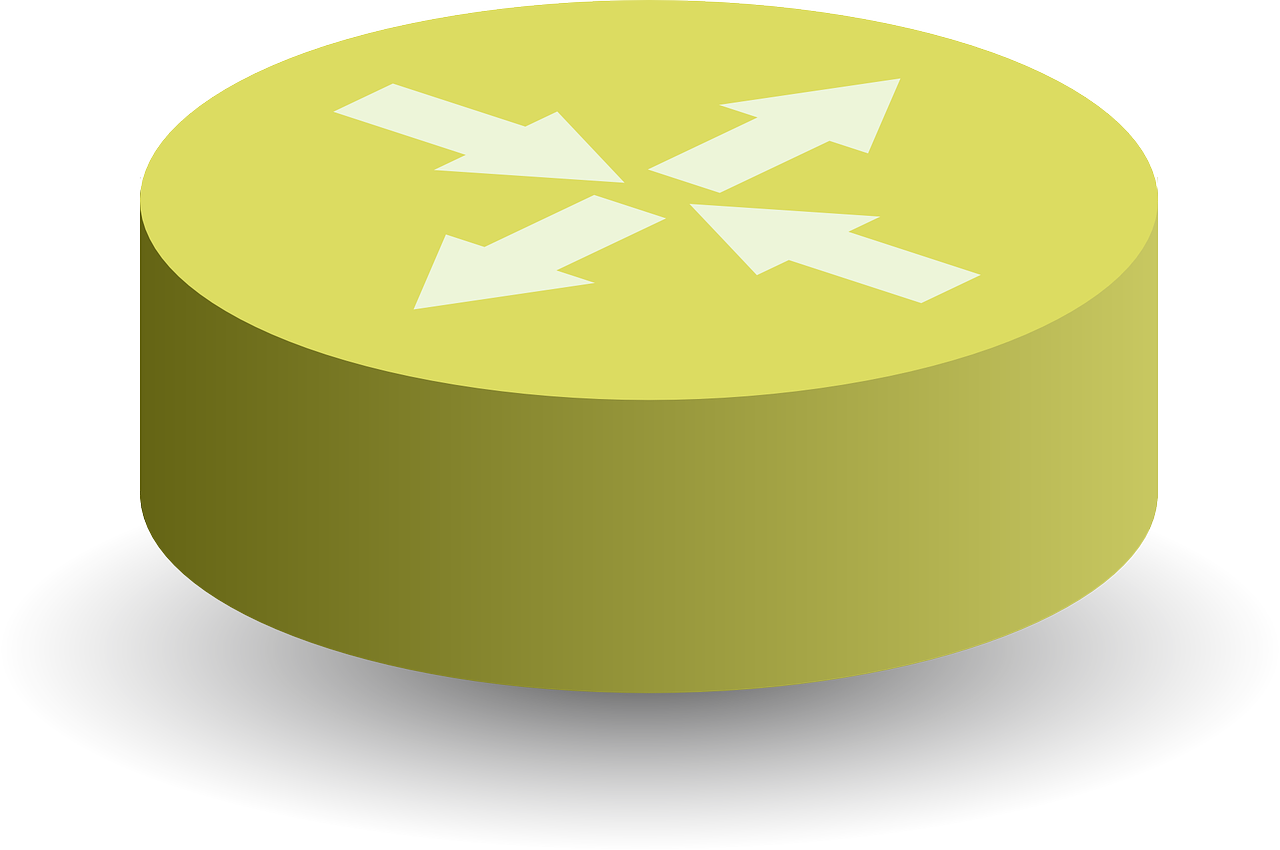
\includegraphics[width=52.5pt,height=52.5pt]{figures/router-158644_1280.png}};
%Image [id:dp12239452759411629] 
\draw (507.5,258.5) node  {\includegraphics[width=52.5pt,height=52.5pt]{figures/router-158644_1280.png}};
%Image [id:dp678906579337467] 
\draw (218.5,413.75) node  {\includegraphics[width=52.5pt,height=52.5pt]{figures/router-158644_1280.png}};
%Image [id:dp34355805397684036] 
\draw (507.5,413.75) node  {\includegraphics[width=52.5pt,height=52.5pt]{figures/router-158644_1280.png}};
%Image [id:dp32408575207048074] 
\draw (360.5,329) node  {\includegraphics[width=52.5pt,height=52.5pt]{figures/router-158644_1280.png}};
%Image [id:dp8786300863621592] 
\draw (218.5,258.5) node  {\includegraphics[width=52.5pt,height=52.5pt]{figures/router-158644_1280.png}};


% Text Node
\draw (221,268) node  [align=left] {A};
% Text Node
\draw (102,338) node  [align=left] {B};
% Text Node
\draw (223,424) node  [align=left] {E};
% Text Node
\draw (364,340) node  [align=left] {C};
% Text Node
\draw (512,271) node  [align=left] {D};
% Text Node
\draw (514,424) node  [align=left] {F};


\end{tikzpicture}

\caption{Network topology of the use case.}
\label{fig:usecase-topo}

\end{figure*}


In addition to the topology, we name the time points of the different steps during the migration process based on the number of iterations (see Figure~\ref{fig:time-points}).
We define the first two basic time points time-0 and time-1 to respectively represent the initial situation and the beginning of the migration process. The last time point varies, depending on the length of execution of the migration.


\begin{figure}[htbp]
\centering
\includegraphics[scale=0.5]{figures/time-points-evolution} 
\caption{Time points of the migration process.\label{fig:time-points}}
\end{figure}

\subsubsection{Initial Situation}
In this section, we consider the network topology prior to any migration.
We solely have the axioms related to the virtual topology, the corresponding users, and the data carried across the network.
We formulate our question to SNARK and verify that the confidentiality is already established prior to the migration (question and answer in Listing~\ref{lst:init-conf-q} and~\ref{lst:init-conf-a}, respectively).

\lstset{numbers=left,numberstyle=\tiny,numbersep=5pt,language=Lisp,
  stringstyle=\ttfamily\small,basicstyle=\ttfamily\footnotesize,
  showstringspaces=false,breaklines=true,keywordstyle=\color{black},}

\begin{lstlisting}[caption=SNARK question to validate the initial situation., label=lst:init-conf-q] 
(find-all '(ans ?d.data ?t.time-interval)
 '(and
 (data-confidentiality ?d.data ?t.time-interval)
(non-empty ?t.time-interval))
 :name 'data-confidentiality-preservation-conjecture
 :num-answers 1
 :time-limit 30  
 :print-derived :print)

;;; search for a data-confidentiality breach:
;;; find all data for which data-confidentiality
;;; has been maintained


(find-all '(ans ?n.node ?t.time-interval)
 '(and
 (node-confidentiality ?n.node ?t.time-interval)
(non-empty ?t.time-interval))
 :name 'node-confidentiality-preservation-conjecture
 :num-answers 1
 :time-limit 30  
 :print-derived :print)

;;; search for a node-confidentiality breach:
;;; find all nodes for which node-confidentiality 
;;; has been maintained
\end{lstlisting}

%\GB{could you comment a bit about what piece of SNARK response  in Lst.~\ref{lst:init-conf-a} gives away the result?}
The interpretation of results provided by SNARK depends on how the question has been formulated.
Lines 1 and 15 from Listing~\ref{lst:init-conf-q} contain requests for the format of the answer.
In these lines, we request SNARK to verify if both nodes and data have their confidentiality respected. The answer will display the time intervals verifying the preservation.
Lines 5 and 15 of Listing~\ref{lst:init-conf-a} hold the answer.
We can establish from line 5 that data-1 has its confidentiality respected (and it is the only one used in our experiment).
At line 15, we have proven that node-1 is not compromised.
The same goes for all the other nodes of the topology, 
for the sake of brevity, these proofs have been omitted.
%but we do not provide the print out in this paper.

\begin{lstlisting}[caption=SNARK validating the initial situation, label=lst:init-conf-a] 
(Row 69
(OR ($$TIME-PP-NOT-BEFORE TIME-0 TIME-1) 
(= (SOME-USER1 DATA-1 (MAKE-INTERVAL TIME-0 TIME-1)) USER-2))
(RESOLVE 66 NON-EMPTY-IF-TIME-POINTS-ORDERED)
Answer (ANS (ANS DATA-1 (MAKE-INTERVAL TIME-0 TIME-1)))) 

(OR ($$TIME-PP-NOT-BEFORE TIME-0 TIME-1)
 (= (SOME-USER1 (SOME-DATA NODE-A (MAKE-INTERVAL TIME-0 TIME-1)) (MAKE-INTERVAL TIME-0 TIME-1)) USER-2)
 (= (SOME-USER NODE-A (MAKE-INTERVAL TIME-0 TIME-1)) USER-2)
 (NOT (DATA-AT-NODE (SOME-DATA NODE-A (MAKE-INTERVAL TIME-0 TIME-1)) NODE-A (MAKE-INTERVAL TIME-0 TIME-1)))
 (NOT
  (DATA-ISAUTHORIZED USER-1 (SOME-DATA NODE-A (MAKE-INTERVAL TIME-0 TIME-1))
   (MAKE-INTERVAL TIME-0 TIME-1))))
   (RESOLVE 115 NON-EMPTY-IF-TIME-POINTS-ORDERED)
   Answer (ANS (ANS NODE-A (MAKE-INTERVAL TIME-0 TIME-1)))) 
\end{lstlisting}


\subsubsection{Information Disclosure attack}
%\GB{are both attacks directed against both migration algorithms}
%\FC{No, but I forgot to mention that we assign an attack per algorithm}
This attack considers two users, one legitimate and one attacker.
The attacker is a collocated user.
In this scenario, the iterative migration algorithm will be used.
During the initial phase, only the legitimate user is active.
The migration process starts and nodes and links are being migrated, one after another.
At some point during the migration, the attacker will start his attack to gain access to the data carried through the VN.
This results into the generation of two predicates, one about the attacker reading the data, and the other about him not being authorized to do so. 
When the migration process ends, the data has been compromised.
In SNARK, the data has been named data-1 and the migration ends at time point time-9.
We formulate our question to SNARK at line 1 from Listing~\ref{lst:not-data-conf-q}.

% \begin{figure}[h]
% \centering
% \includegraphics[scale=0.5]{not-data-confidentiality-question}
% \caption{SNARK question to detect the data confidentiality violation.\label{fig:not-data-conf-q}}
% \end{figure}
% \begin{figure}[h]
% \centering
% \includegraphics[scale=0.5]{not-data-confidentiality-answer}
% \caption{SNARK detecting the data confidentiality violation\label{fig:not-data-conf-a}}
% \end{figure}
\begin{lstlisting}[caption=SNARK question to detect the data confidentiality violation., label=lst:not-data-conf-q] 
   (find-all '(ans ?d.data ?t.time-interval)
             '(and
       (not(data-confidentiality ?d.data ?t.time-interval))
         (non-empty ?t.time-interval))
         :name 'data-conf-preservation-conjecture
         :num-answers 1
         :time-limit 30
         :print-derived :print)
;;; search for a data-confidentiality breach:
;;; find all data for which data-confidentiality has been maintained

\end{lstlisting}
\begin{lstlisting}[caption=SNARK detecting the data confidentiality violation., label=lst:not-data-conf-a] 
(Row 2112  
(OR
 (NOT
  (= (MAKE-INTERVAL TIME-0 ?X.TIME-POINT)
   (MAKE-INTERVAL (MAX-TIME ?Y.TIME-POINT ?Z.TIME-POINT) (MIN-TIME ?U.TIME-POINT ?V.TIME-POINT))))
 (NOT (SETLINK0 NODE-B ?W.NODE (MAKE-INTERVAL ?Y.TIME-POINT ?U.TIME-POINT)))
 (NOT (SETLINK ?W.NODE NODE-A (MAKE-INTERVAL ?Z.TIME-POINT ?V.TIME-POINT)))
 ($$TIME-PP-NOT-BEFORE TIME-9 (MIN-TIME TIME-1 ?X.TIME-POINT)) ($$TIME-PP-NOT-BEFORE TIME-4 TIME-9)
 (NOT (= (MAKE-INTERVAL TIME-4 TIME-9) (MAKE-INTERVAL TIME-0 TIME-9))) ($$TIME-PP-NOT-BEFORE TIME-4 TIME-9)
 (DATA-ISAUTHORIZED ATTACKER DATA-1 (MAKE-INTERVAL TIME-4 TIME-9)))
   (RESOLVE 1938 18)
   Answer (ANS (ANS DATA-1 (MAKE-INTERVAL TIME-4 TIME-9)))) 
\end{lstlisting}
We can see that SNARK confirms the data confidentiality violation at line 12 from Listing~\ref{lst:not-data-conf-a}.
Since the attack started during the migration (i.e after time point time-1), SNARK detects the beginning of the confidentiality violation at time point time-4.
Line 10 highlights that the attacker does not have the authorization to read the data.
%\GB{could you point out directly which line you are referring to by labeling and referring to independent lines in the listing?}

\subsubsection{Migration alteration attack}
Exploiting the physical nodes leverages other aspects of the security the infrastructure.
The initial situation is similar to the previous scenario but we use the move-based migration algorithm instead.
The attacker is located in the network infrastructure.
The attacker can render physical nodes unavailable to trigger the migration process and will intercept and modify the configuration data sent by the hypervisor. 
Therefore, the $conf\_integrity$ property does not hold true anymore.
%\GB{should this fact be generated. Should this be rather the absence of an is\_authorized predicate that would indicate the attack?}
%\FC{Answered by email}
At line 1 in Listing~\ref{lst:not-conf-int-q}, we ask SNARK to find all the nodes in which there is an integrity breach for their configuration.

\begin{lstlisting}[caption=SNARK question to detect the configuration integrity violation., label=lst:not-conf-int-q,captionpos=b] 
   (find-all '(ans ?n.node ?t.time-interval)
             '(and
       (not(conf-integrity ?d.data ?n.node ?t.time-interval))
               (non-empty ?t.time-interval))
             :name 'conf-int-violation-conjecture
             :num-answers 1
             :time-limit 30
                     :print-derived :print)
   ;;; search for a configuration integrity breach:
   ;;; find all nodes for which conf-integrity has not been maintained
\end{lstlisting}
The configuration integrity breach is then proven by SNARK for new\_node-a (the first migrated node) at line 3 in Listing~\ref{lst:not-conf-int-a}.
Similarly to the previous information disclosure scenario, the attack starts after the beginning of the migration process.
SNARK finds the beginning of the attack on node-a starting at time point time-1.
%\GB{again, please provide line numbers for the reviewer to ``see something''}

\begin{lstlisting}[caption=SNARK detecting the configuration integrity violation., label=lst:not-conf-int-a,captionpos=b] 
(AND (DATA-INTEGRITY DATA-CONF (MAKE-INTERVAL TIME-1 ?X.TIME-POINT))
 ($$TIME-PP-NOT-AFTER ?X.TIME-POINT TIME-3))
   Answer (ANS (ANS NEW_NODE-A (MAKE-INTERVAL TIME-1 TIME-3)))) 
\end{lstlisting}

The proof related to the other security properties is identical in essence, thus we do not include it here.

\newpage
\subsection{Conclusion}
    In this chapter we have presented a formal model describing a virtualization infrastructure, the embedding of virtual resources on top of a physical substrate, the evolution of such embedding during the migration of a virtual network and a set of security properties. These properties were addressed by considering them in a very general way, and then refining them more precisely into a SDN context. We have proposed to evaluate the formal model with real life use cases, considering attacks existing on SDN infrastructures, and using a simulator to generate the execution trace. Finally, we used the theorem prover SNARK to compute a formal proof of the security violation during the migration.

Our analysis of the state of the art has outlined a lack of consideration for the security study of the migration process of a virtual network.
One logical explanation is that the migration process is rarely implemented in a network hypervisor, especially because this process corresponds to operational needs and that there is only a limited number of commercial solutions for SDN.
Our results demonstrate the possibility of formally proving the preservation or the violation of the security properties, based on the analysis of an execution trace.

Despite the fact that the co-residency is a security property that cannot be violated \textit{per se}, we define it to illustrate the evolution of the attack surface that can be exploited to compromise the operation of the migration process, as it is done for traditional hypervisors~\cite{stalling-atya2017,malicious-atya2017}.
Abnormal behaviours could be detected using co-residency and attackers could be exposed for trying be located on the same physical resources as their victim. 

The use of a formal approach to verify real life problems inevitably raises a question about the coherence between the model and its reality.
In our case, we prove that we can detection security violations, but this comes with the underlying hypotheses that we can detect and characterize every relevant network event and that the trace generated from the migration is complete. However, we are left with the challenge to alleviate the hypothesis that the security tool is omnipotent and will never miss any event that would pertain to the proof. As it is, this assumption is too strong for a real life use of our solution.

In the next chapter, we propose to tackle this issue by proposing a resource allocation model that will optimize the coverage of the security monitoring inside the infrastructure.

\newpage
\section{Optimizing resource allocation of monitoring resources}
\label{sec:RAprob}
\subsection{Motivation}
In the previous chapter we have presented a formal model describe several security aspects of an SDN virtualization infrastructure, and more precisely we considered the virtual network migration process as a specific context in the virtualization.

We made several assumptions for this work, and one of the strongest is the perfect knowledge of the events in the network infrastructure. The proof given by the formal model relies on the fact that we have a complete knowledge of all the events that happened during the migration. As we have explained why during the experimental evaluation of our formal model that assumption holds. However, this assumption is too strong to be considered in a real life environment. Current IDS solutions cannot ensure that all attacks and events impacting the migration can be detected, therefore the perfect knowledge assumption does not hold.

We propose to alleviate this hypothesis for a real life use case with an optimization model for the deployment of the monitoring in the infrastructure.
We consider a virtualization infrastructure, and want to improve the security of the migration process.
Monitoring solutions incur a financial cost for the service provider, as well as a performance impact because computing resources are not dedicated to the virtualization service.
The main objective is to determine which nodes in the infrastructure should support the monitoring function.
The optimal deployment should consider the attacks launched on the migration.
The problem considered here is a typical instance of the resource allocation problem.

Several solution for the resource allocation are presented in the state of the art. 
Linear Programming models the system with a set of equations, and maximize a reward function under a set of constraints.
The main drawback in solving security resource allocation problems with Linear Programming is the lack of consideration for the attacker's capacities in the solution.

The Game Theory formalism is at the other end of the spectrum, where the behavior of both the infrastructure owner and the attacker can be modeled.
The formalism provides different types of games, each corresponding to particular situations and how players choose their action.
Game Theory does not explore the resource allocation problem in an SDN environment, and we expect some applicability in our study.

Markov Decision Processes sit between linear programming and Game Theory, where the model only considers the perspective of one entity, but gives the entity actions to make to interact with the system. The resource allocation problem is not well studied using MDP, but it provides enough granularity in the actions and the transition model to be worth investigating.






\newpage
\subsection{Game Theory}
\section{First approach: Game Theory}

We investigate the resource allocation problem previously described with the formalism of Game Theory.
We consider a two-player game, where one player is the attacker and targets the infrastructure to gain access to confidential data. The other player is the infrastructure owner, also referred to as ``the defender'' for the rest of this chapter.
We will present the assumptions we made, then describe the players and their associated strategies, and finally discuss the different types of games we have considered.

\subsection{Objectives of the game}
Regardless of the type of game considered, we investigated the formalism with the following idea in mind: ``Can we optimize the monitoring with alternative strategies like decoys or Moving Target Defense ?''\GB{but the question is whether you are attempting to answer the same problem with MDP or not. And if not (as it seems the problem is no more about RA), you need to justify what prompted you to consider a different problem.}\FC{I rephrased correctly}.
The solution of the game is supposed to show whether or not the defender can benefit from these techniques. Precisely, we consider that setting up a decoy in the infrastructure is lest costly than permanently monitoring the infrastructure. We want to determine if using a cheap alternative defense technique is more efficient than using a costly monitoring solution.
In a similar way, we want to determine if the attacker should do an extensive information collection phase prior to actually attacking the infrastructure, or if the use of decoys is not going to be an effective method to prevent the attacker from attacking blindly.



\subsection{Assumptions}
We have made several assumptions about the scope of the game:
\begin{description}
\item \textbf{Migration: } The migration has already started when the game starts.
\item \textbf{Constrained budgets: } Both players have limited capacities to either attack or defend the infrastructure.
This implies that the whole infrastructure cannot be attacked or defended.
\item \textbf{Complete information: } The game is considered to be of complete information.
\end{description}

\subsection{Defender}
The goal of the defender is to protect his infrastructure by either deploying monitoring or decoy on nodes. A decoy node contains flow rules that will mislead the attacker into believing the node is part of the new embedding of the migrated network.

The defender can choose among three different strategies:
\begin{description}
\item \textbf{Installing a decoy: } The defender installs flow rules in a node that will hold information related to the migrated network but the node will in fact not be used to embed the Virtual Network.
\item \textbf{Monitoring a node: } The defender deploys monitoring on the node to contribute to the detection.
\item \textbf{Doing nothing}.
\end{description}

\subsection{Attacker}
The attacker will compromise the migration to gain access to his victim's sensitive data.
The attack is performed by installing flow rules in specific nodes that will allow him to duplicate the victim's traffic towards one of his Virtual Machines, as depicted in Figure~\ref{fig:data-exfiltration-attack}. 
The attacker will compromise several nodes in order to establish a path between his victim's VN and one of his own VMs.
He will then use the compromised nodes to duplicate the victim's network traffic and redirect it towards his VM.
The attack is considered complete when all the nodes establishing the full unauthorized path have been compromised.

The attacker's features are as follows:
\begin{description}
\item \textbf{Location: } The attacker has compromised one node in the infrastructure.
\item \textbf{Resources: } The attacker owns Virtual Machines in the infrastructure.
\item \textbf{Capacities: } The attacker can scan or attack any node in the infrastructure.
\item \textbf{Knowledge about the victim: } The attacker can identify the flow rules belonging to his victim.
\item \textbf{Knowledge about the infrastructure: } The attacker has the view of the whole physical infrastructure.
\item \textbf{Knowledge about the embedding: } The attacker does not know the new embedding for his victim's Virtual Network.
\end{description}

The attacker can choose among three different strategies:
\begin{description}
\item \textbf{Scanning a node: } The attacker can request the list of  flow rules installed in a node. This allows him to discover the embedding location of his victim.
\item \textbf{Attacking a node: } The attacker will install in a node specific rules to construct the path between his VM and the victim's Virtual Network.
\item \textbf{Doing nothing}.
\end{description}



\subsection{Games considered to solve the RA problem}
We have considered several types of games for this problem, and we will present their limitations and impact.

\paragraph{Static games} These games are played on each node of the infrastructure, only once. We investigated a game based on the works of Ismail~\etal~\cite{Chen2009,interdep-ismail2017}. The immediate limitation of this game is the inadequacy to use scans and decoys as the attacker is supposed to leverage the information collected to improve his next attack. This leaves us with a model where the attacker either attacks a node or not, and where the defender takes a similar stance, either defending the node or not.

The second limitation of static games is their inadequacy to represent the migration process as a succession of steps, where the system would become more and more worth attacking because the number of nodes holding valuable information would increase as the migration goes on.

% The work of Ismail~\etal takes the Game Theory formalism far in the modeling, and focuses on several aspects of an infrastructure running on a legacy network. The opportunity here is to add the representation of SDN and the decoupling of the control plane and the data plane in the model.

These limitations convinced us that static games were not a fruitful lead to investigate.
We draw the same conclusion for repeated games, as these are static games repeated several times without any change in the way the game is played.

% \textbf{Repeated games: } These games are static games played several times.
% Since the game must remain unchanged at every play, the limitations encountered woth static games still apply here. 

\paragraph{Sequential games} These games represent players taking turns choosing their action. This aspect makes them more interesting to consider than static games, because the migration process can be represented along the choices made by players. In this situation, the complete information aspect of the game can still be maintained, but the idea of using decoys in the infrastructure requires an imperfect information game. The location of decoys must remain unknown to the attacker to be effective.
Indeed, if the attacker knows where the decoys are deployed he will not attack these nodes.

The main limitation encountered here is that the choice of all players must be revealed after every player has chosen his strategy. Therefore, it is impossible to accumulate rounds without revealing the defender's actions to the attacker. This makes the use of decoys worthless and limits the game to a simple attack/defend/do nothing scheme, similarly to static games.

\paragraph{Stochastic games} Modeling the evolution of a system based on the choices made by players is an interesting formalism for our problem. We can consider the evolution of the infrastructure as the migration process goes on, as well as the progress of the attacker to exfiltrate the data. 

The costs of the strategies are different for the attacker and the defender, thus making the game a non zero-sum stochastic game. Non zero-sum stochastic games with imperfect information turn out to be widely complex to solve, and, to the best of our knowledge, there is no algorithm that can be used as a support for the resolution of a network security problem\GB{isn't it an RA problem?}\FC{I don't understand the question}. 

Additionally, considering a zero-sum stochastic game would make the computation of the equilibrium tractable but at the expense of the game's realism.
% \GB{I feel that the last sentences below this comment should be featured in the discussion.}


\subsection{Discussion}
We have reviewed several types of games in this section, where each type has its own share of limitations regarding our problem. Another aspect that we have not detailed before is the acceptable granularity of actions for the players. Indeed, the vast majority of work we have surveyed in Chapter~\ref{sec:sota} limits the players to a binary choice: attacking/defending or doing nothing. This reduced number of choices leaves us with the concern of whether we are allowed to define precise strategies for a security game, or if each strategy must be significantly different from every other~\cite{Kiennert2018}. 
This also raises the question of the validity of the complete information assumption.
This assumption is common in network security games, which may not be realistic in real-life scenarios.
While an attacker will expect monitoring counter-measures in the infrastructure, it is not trivial to assume that the attacker knows about the specificity of the counter-measures deployed in the infrastructure, especially if their nature deviate from standard IDS solutions (\eg decoys and Moving Target Defense).
% Finally, depending on the type of game chosen, the realism of the modeling is also heavily impacted because of the assumptions made about the system to protect.
% as well as the arbitrary choices made for the costs and rewards.
% In the state of the art, the values chosen in the utility functions rarely are evaluated using a real life methodology, especially on the attacker side where the literature is very scarce. 
This leaves us with the question: ``Are existing types of games coherent and realistic with current real-life use cases ?''.

We conclude this section with the observation that Game Theory does not offer enough flexibility to model our problem. 

We prefer to consider the formalism of Markov Decision Processes (MDP), which have a similar nature to stochastic games. MDPs are more flexible because a single agent is interacting with the system, and the perfect information aspect of game theory is not relevant in this context. 
In the next chapter, we explore the use of Markov Decision Processes and illustrate how this formalism can be used to include the consequences of attacks in the strategy of the defender.


\newpage
\subsection{Markov Decision Process}
\section{Second approach: Markov Decision Process}
We have considered the formalism of Game Theory as a method to solve the resource allocation problem, but the lack of flexibility and the complexity of determining the equilibrium make it inadequate for our problem. We consider here Markov Decision Processes (MDP).
MDP is a formalism used to represent an agent and the actions he can choose to interact with a system. The general purpose of an MDP is to find the best action for each possible state of the system (\ie the optimal policy). Because a practical solution to this RA problem is a set of nodes supporting the monitoring of the infrastructure, we will develop a statistical analysis of the optimal policy and convert the dynamic answer of a MDP into a static \textit{a priori} deployment.
An experimental prototype is available on github\footnote{\label{github}\url{https://github.com/FabienCharmet/MDPRA}}.


% \label{sec:mdp-reqiorements}
We formulate the following requirements regarding the formalization of the MDP:\\
\textbf{Solution form: } The solution to the problem is the optimal set of nodes to monitor the infrastructure.\\
\textbf{Constrained budgets: } The defender has a limited financial budget and a maximum performance impact threshold.
This implies that the whole infrastructure cannot be defended.\\
\textbf{Specific attacks: } The attack on the migration process must be fine grained and target specific nodes.


\begin{figure*}[ht]

\tikzset{every picture/.style={line width=0.75pt}} %set default line width to 0.75pt        

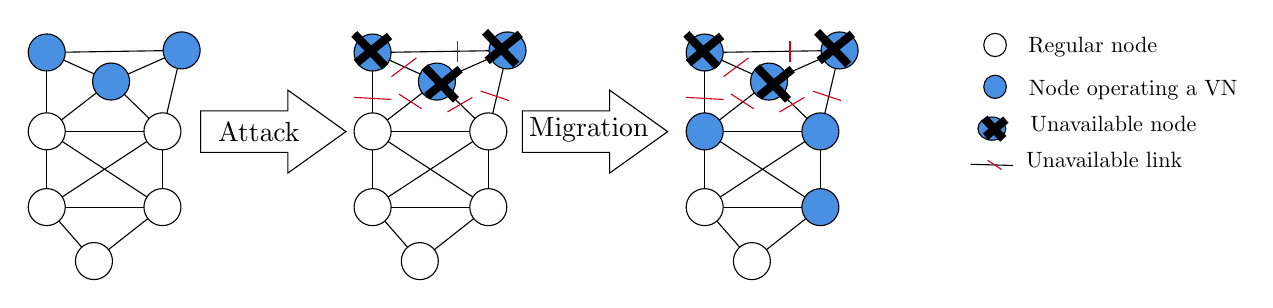
\begin{tikzpicture}[x=0.75pt,y=0.75pt,yscale=-1,xscale=1]
%uncomment if require: \path (0,300); %set diagram left start at 0, and has height of 300

%Shape: Ellipse [id:dp8430130954948494] 
\draw  [fill={rgb, 255:red, 74; green, 144; blue, 226 }  ,fill opacity=1 ] (461.48,51.56) .. controls (461.48,48.47) and (464.48,45.97) .. (468.19,45.97) .. controls (471.9,45.97) and (474.9,48.47) .. (474.9,51.56) .. controls (474.9,54.66) and (471.9,57.16) .. (468.19,57.16) .. controls (464.48,57.16) and (461.48,54.66) .. (461.48,51.56) -- cycle ;
%Shape: Ellipse [id:dp5907962461562573] 
\draw  [fill={rgb, 255:red, 74; green, 144; blue, 226 }  ,fill opacity=1 ] (464.29,31.43) .. controls (464.29,28.34) and (466.73,25.83) .. (469.74,25.83) .. controls (472.75,25.83) and (475.19,28.34) .. (475.19,31.43) .. controls (475.19,34.52) and (472.75,37.02) .. (469.74,37.02) .. controls (466.73,37.02) and (464.29,34.52) .. (464.29,31.43) -- cycle ;
%Straight Lines [id:da1514909222057811] 
\draw [color={rgb, 255:red, 0; green, 0; blue, 0 }  ,draw opacity=1 ]   (458,68.75) -- (478.38,69.32) ;


%Shape: Ellipse [id:dp8047559285598944] 
\draw  [fill={rgb, 255:red, 255; green, 255; blue, 255 }  ,fill opacity=1 ] (464.29,11.26) .. controls (464.29,8.17) and (466.73,5.67) .. (469.74,5.67) .. controls (472.75,5.67) and (475.19,8.17) .. (475.19,11.26) .. controls (475.19,14.35) and (472.75,16.86) .. (469.74,16.86) .. controls (466.73,16.86) and (464.29,14.35) .. (464.29,11.26) -- cycle ;
%Straight Lines [id:da5581047744563914] 
\draw [color={rgb, 255:red, 208; green, 2; blue, 27 }  ,draw opacity=1 ]   (472.87,71.26) -- (466.14,66.8) ;


%Straight Lines [id:da6983464143799673] 
\draw [line width=3]    (464.54,46.62) -- (473.71,56.51) ;


%Straight Lines [id:da20248481970311139] 
\draw [line width=3]    (465.15,55.41) -- (474.93,47.25) ;



%Straight Lines [id:da6176709448343998] 
\draw    (200.83,28.91) -- (225.58,52.91) ;


%Straight Lines [id:da5463688705908274] 
\draw    (200.83,28.91) -- (169.83,52.91) ;


%Straight Lines [id:da11538810799649779] 
\draw    (234.83,13.91) -- (225.92,51.91) ;


%Straight Lines [id:da8853756126147032] 
\draw    (169.83,14.91) -- (169.83,52.91) ;


%Straight Lines [id:da5031310157957251] 
\draw    (169.83,52.91) -- (225.58,89.41) ;


%Straight Lines [id:da8400043886929478] 
\draw    (169.83,89.41) -- (192.58,115.41) ;


%Straight Lines [id:da5242150334882041] 
\draw    (225.58,89.41) -- (192.58,115.41) ;


%Straight Lines [id:da3960630757961663] 
\draw    (225.58,52.91) -- (169.83,89.41) ;


%Shape: Circle [id:dp47175232960651714] 
\draw  [fill={rgb, 255:red, 255; green, 255; blue, 255 }  ,fill opacity=1 ] (160.92,52.91) .. controls (160.92,47.98) and (164.91,43.99) .. (169.83,43.99) .. controls (174.76,43.99) and (178.75,47.98) .. (178.75,52.91) .. controls (178.75,57.83) and (174.76,61.82) .. (169.83,61.82) .. controls (164.91,61.82) and (160.92,57.83) .. (160.92,52.91) -- cycle ;
%Shape: Circle [id:dp5879580381901867] 
\draw  [fill={rgb, 255:red, 255; green, 255; blue, 255 }  ,fill opacity=1 ] (216.67,52.91) .. controls (216.67,47.98) and (220.66,43.99) .. (225.58,43.99) .. controls (230.51,43.99) and (234.5,47.98) .. (234.5,52.91) .. controls (234.5,57.83) and (230.51,61.82) .. (225.58,61.82) .. controls (220.66,61.82) and (216.67,57.83) .. (216.67,52.91) -- cycle ;
%Shape: Circle [id:dp5579759383684684] 
\draw  [fill={rgb, 255:red, 255; green, 255; blue, 255 }  ,fill opacity=1 ] (160.92,89.41) .. controls (160.92,84.48) and (164.91,80.49) .. (169.83,80.49) .. controls (174.76,80.49) and (178.75,84.48) .. (178.75,89.41) .. controls (178.75,94.33) and (174.76,98.32) .. (169.83,98.32) .. controls (164.91,98.32) and (160.92,94.33) .. (160.92,89.41) -- cycle ;
%Shape: Circle [id:dp885869190555082] 
\draw  [fill={rgb, 255:red, 255; green, 255; blue, 255 }  ,fill opacity=1 ] (216.67,89.41) .. controls (216.67,84.48) and (220.66,80.49) .. (225.58,80.49) .. controls (230.51,80.49) and (234.5,84.48) .. (234.5,89.41) .. controls (234.5,94.33) and (230.51,98.32) .. (225.58,98.32) .. controls (220.66,98.32) and (216.67,94.33) .. (216.67,89.41) -- cycle ;
%Shape: Circle [id:dp3254884021888832] 
\draw  [fill={rgb, 255:red, 255; green, 255; blue, 255 }  ,fill opacity=1 ] (183.67,115.41) .. controls (183.67,110.48) and (187.66,106.49) .. (192.58,106.49) .. controls (197.51,106.49) and (201.5,110.48) .. (201.5,115.41) .. controls (201.5,120.33) and (197.51,124.32) .. (192.58,124.32) .. controls (187.66,124.32) and (183.67,120.33) .. (183.67,115.41) -- cycle ;
%Straight Lines [id:da7041582060743201] 
\draw    (178.75,52.91) -- (216.67,52.91) ;


%Straight Lines [id:da26176464493068274] 
\draw    (178.75,89.41) -- (216.67,89.41) ;


%Straight Lines [id:da45312150436944487] 
\draw    (225.58,80.49) -- (225.58,61.82) ;


%Straight Lines [id:da10497643854199257] 
\draw    (169.83,61.82) -- (169.83,80.49) ;


%Straight Lines [id:da023464273570334315] 
\draw    (169.83,14.91) -- (234.83,13.91) ;


%Straight Lines [id:da7461511731963238] 
\draw    (200.83,28.91) -- (234.83,13.91) ;


%Straight Lines [id:da6717008743630867] 
\draw    (169.83,14.91) -- (200.83,28.91) ;


%Shape: Circle [id:dp17672294199894456] 
\draw  [fill={rgb, 255:red, 74; green, 144; blue, 226 }  ,fill opacity=1 ] (160.92,14.91) .. controls (160.92,9.98) and (164.91,5.99) .. (169.83,5.99) .. controls (174.76,5.99) and (178.75,9.98) .. (178.75,14.91) .. controls (178.75,19.83) and (174.76,23.82) .. (169.83,23.82) .. controls (164.91,23.82) and (160.92,19.83) .. (160.92,14.91) -- cycle ;
%Shape: Circle [id:dp8878711028556632] 
\draw  [fill={rgb, 255:red, 74; green, 144; blue, 226 }  ,fill opacity=1 ] (191.92,28.91) .. controls (191.92,23.98) and (195.91,19.99) .. (200.83,19.99) .. controls (205.76,19.99) and (209.75,23.98) .. (209.75,28.91) .. controls (209.75,33.83) and (205.76,37.82) .. (200.83,37.82) .. controls (195.91,37.82) and (191.92,33.83) .. (191.92,28.91) -- cycle ;
%Shape: Circle [id:dp02560438280336974] 
\draw  [fill={rgb, 255:red, 74; green, 144; blue, 226 }  ,fill opacity=1 ] (225.92,13.91) .. controls (225.92,8.98) and (229.91,4.99) .. (234.83,4.99) .. controls (239.76,4.99) and (243.75,8.98) .. (243.75,13.91) .. controls (243.75,18.83) and (239.76,22.82) .. (234.83,22.82) .. controls (229.91,22.82) and (225.92,18.83) .. (225.92,13.91) -- cycle ;
%Straight Lines [id:da7816159630212767] 
\draw [color={rgb, 255:red, 208; green, 2; blue, 27 }  ,draw opacity=1 ]   (210.92,9.51) -- (210.92,19.51) ;


%Straight Lines [id:da23242280473047117] 
\draw [color={rgb, 255:red, 208; green, 2; blue, 27 }  ,draw opacity=1 ]   (221.92,33.51) -- (235.5,38.01) ;


%Straight Lines [id:da25217250177313655] 
\draw [color={rgb, 255:red, 208; green, 2; blue, 27 }  ,draw opacity=1 ]   (160.92,36.51) -- (178.92,37.51) ;


%Straight Lines [id:da8252457737222165] 
\draw [color={rgb, 255:red, 208; green, 2; blue, 27 }  ,draw opacity=1 ]   (178.92,26.51) -- (190.92,17.51) ;


%Straight Lines [id:da6307655523636441] 
\draw [color={rgb, 255:red, 208; green, 2; blue, 27 }  ,draw opacity=1 ]   (205.92,43.51) -- (217.92,36.51) ;


%Straight Lines [id:da5703265914230616] 
\draw [color={rgb, 255:red, 208; green, 2; blue, 27 }  ,draw opacity=1 ]   (193.5,42.01) -- (182.5,34.91) ;


%Straight Lines [id:da3989594608358942] 
\draw [line width=3]    (161,5.93) -- (176,21.68) ;


%Straight Lines [id:da7318288975856456] 
\draw [line width=3]    (162,19.93) -- (178,6.93) ;



%Straight Lines [id:da9963706937012238] 
\draw [line width=3]    (224,4.93) -- (239,20.68) ;


%Straight Lines [id:da43798340024618054] 
\draw [line width=3]    (225,18.93) -- (241,5.93) ;



%Straight Lines [id:da5033136183613764] 
\draw [line width=3]    (195,21.93) -- (210,37.68) ;


%Straight Lines [id:da623542865534238] 
\draw [line width=3]    (196,35.93) -- (212,22.93) ;




%Straight Lines [id:da021425369536150374] 
\draw    (43.83,28.87) -- (68.58,52.87) ;


%Straight Lines [id:da809644771756096] 
\draw    (43.83,28.87) -- (12.83,52.87) ;


%Straight Lines [id:da9075994171710501] 
\draw    (77.83,13.87) -- (68.92,51.87) ;


%Straight Lines [id:da7475460187374237] 
\draw    (12.83,14.87) -- (12.83,52.87) ;


%Straight Lines [id:da06975692875380135] 
\draw    (12.83,52.87) -- (68.58,89.37) ;


%Straight Lines [id:da9394544948671463] 
\draw    (12.83,89.37) -- (35.58,115.37) ;


%Straight Lines [id:da46361116523850066] 
\draw    (68.58,89.37) -- (35.58,115.37) ;


%Straight Lines [id:da9816638193583865] 
\draw    (68.58,52.87) -- (12.83,89.37) ;


%Shape: Circle [id:dp21531756732058427] 
\draw  [fill={rgb, 255:red, 255; green, 255; blue, 255 }  ,fill opacity=1 ] (3.92,52.87) .. controls (3.92,47.95) and (7.91,43.96) .. (12.83,43.96) .. controls (17.76,43.96) and (21.75,47.95) .. (21.75,52.87) .. controls (21.75,57.8) and (17.76,61.79) .. (12.83,61.79) .. controls (7.91,61.79) and (3.92,57.8) .. (3.92,52.87) -- cycle ;
%Shape: Circle [id:dp32258921480580105] 
\draw  [fill={rgb, 255:red, 255; green, 255; blue, 255 }  ,fill opacity=1 ] (59.67,52.87) .. controls (59.67,47.95) and (63.66,43.96) .. (68.58,43.96) .. controls (73.51,43.96) and (77.5,47.95) .. (77.5,52.87) .. controls (77.5,57.8) and (73.51,61.79) .. (68.58,61.79) .. controls (63.66,61.79) and (59.67,57.8) .. (59.67,52.87) -- cycle ;
%Shape: Circle [id:dp7783815840311967] 
\draw  [fill={rgb, 255:red, 255; green, 255; blue, 255 }  ,fill opacity=1 ] (3.92,89.37) .. controls (3.92,84.45) and (7.91,80.46) .. (12.83,80.46) .. controls (17.76,80.46) and (21.75,84.45) .. (21.75,89.37) .. controls (21.75,94.3) and (17.76,98.29) .. (12.83,98.29) .. controls (7.91,98.29) and (3.92,94.3) .. (3.92,89.37) -- cycle ;
%Shape: Circle [id:dp9106798970146953] 
\draw  [fill={rgb, 255:red, 255; green, 255; blue, 255 }  ,fill opacity=1 ] (59.67,89.37) .. controls (59.67,84.45) and (63.66,80.46) .. (68.58,80.46) .. controls (73.51,80.46) and (77.5,84.45) .. (77.5,89.37) .. controls (77.5,94.3) and (73.51,98.29) .. (68.58,98.29) .. controls (63.66,98.29) and (59.67,94.3) .. (59.67,89.37) -- cycle ;
%Shape: Circle [id:dp1831427544072476] 
\draw  [fill={rgb, 255:red, 255; green, 255; blue, 255 }  ,fill opacity=1 ] (26.67,115.37) .. controls (26.67,110.45) and (30.66,106.46) .. (35.58,106.46) .. controls (40.51,106.46) and (44.5,110.45) .. (44.5,115.37) .. controls (44.5,120.3) and (40.51,124.29) .. (35.58,124.29) .. controls (30.66,124.29) and (26.67,120.3) .. (26.67,115.37) -- cycle ;
%Straight Lines [id:da9700158448121917] 
\draw    (21.75,52.87) -- (59.67,52.87) ;


%Straight Lines [id:da010185511635833033] 
\draw    (21.75,89.37) -- (59.67,89.37) ;


%Straight Lines [id:da4677014236726348] 
\draw    (68.58,80.46) -- (68.58,61.79) ;


%Straight Lines [id:da19862578341507608] 
\draw    (12.83,61.79) -- (12.83,80.46) ;


%Straight Lines [id:da6877311034443738] 
\draw    (12.83,14.87) -- (77.83,13.87) ;


%Straight Lines [id:da39601253001890035] 
\draw    (43.83,28.87) -- (77.83,13.87) ;


%Straight Lines [id:da8270994037474519] 
\draw    (12.83,14.87) -- (43.83,28.87) ;


%Shape: Circle [id:dp2984826737185816] 
\draw  [fill={rgb, 255:red, 74; green, 144; blue, 226 }  ,fill opacity=1 ] (3.92,14.87) .. controls (3.92,9.95) and (7.91,5.96) .. (12.83,5.96) .. controls (17.76,5.96) and (21.75,9.95) .. (21.75,14.87) .. controls (21.75,19.8) and (17.76,23.79) .. (12.83,23.79) .. controls (7.91,23.79) and (3.92,19.8) .. (3.92,14.87) -- cycle ;
%Shape: Circle [id:dp6437572475375565] 
\draw  [fill={rgb, 255:red, 74; green, 144; blue, 226 }  ,fill opacity=1 ] (34.92,28.87) .. controls (34.92,23.95) and (38.91,19.96) .. (43.83,19.96) .. controls (48.76,19.96) and (52.75,23.95) .. (52.75,28.87) .. controls (52.75,33.8) and (48.76,37.79) .. (43.83,37.79) .. controls (38.91,37.79) and (34.92,33.8) .. (34.92,28.87) -- cycle ;
%Shape: Circle [id:dp23183818676236623] 
\draw  [fill={rgb, 255:red, 74; green, 144; blue, 226 }  ,fill opacity=1 ] (68.92,13.87) .. controls (68.92,8.95) and (72.91,4.96) .. (77.83,4.96) .. controls (82.76,4.96) and (86.75,8.95) .. (86.75,13.87) .. controls (86.75,18.8) and (82.76,22.79) .. (77.83,22.79) .. controls (72.91,22.79) and (68.92,18.8) .. (68.92,13.87) -- cycle ;

%Right Arrow [id:dp417684980473099] 
\draw   (87,43) -- (129,43) -- (129,33) -- (157,53) -- (129,73) -- (129,63) -- (87,63) -- cycle ;

%Right Arrow [id:dp6623970589974628] 
\draw   (242,43) -- (284,43) -- (284,33) -- (312,53) -- (284,73) -- (284,63) -- (242,63) -- cycle ;
%Straight Lines [id:da22163993557127015] 
\draw    (360.83,28.91) -- (385.58,52.91) ;


%Straight Lines [id:da8341652491193966] 
\draw    (360.83,28.91) -- (329.83,52.91) ;


%Straight Lines [id:da14662408338887967] 
\draw    (394.83,13.91) -- (385.92,51.91) ;


%Straight Lines [id:da1054361182628697] 
\draw    (329.83,14.91) -- (329.83,52.91) ;


%Straight Lines [id:da878058282787745] 
\draw    (329.83,52.91) -- (385.58,89.41) ;


%Straight Lines [id:da5143639640863213] 
\draw    (329.83,89.41) -- (352.58,115.41) ;


%Straight Lines [id:da38106162801473] 
\draw    (385.58,89.41) -- (352.58,115.41) ;


%Straight Lines [id:da9515281954413589] 
\draw    (385.58,52.91) -- (329.83,89.41) ;


%Shape: Circle [id:dp7012949201072771] 
\draw  [fill={rgb, 255:red, 74; green, 144; blue, 226 }  ,fill opacity=1 ] (320.92,52.91) .. controls (320.92,47.98) and (324.91,43.99) .. (329.83,43.99) .. controls (334.76,43.99) and (338.75,47.98) .. (338.75,52.91) .. controls (338.75,57.83) and (334.76,61.82) .. (329.83,61.82) .. controls (324.91,61.82) and (320.92,57.83) .. (320.92,52.91) -- cycle ;
%Shape: Circle [id:dp8511635916765001] 
\draw  [fill={rgb, 255:red, 74; green, 144; blue, 226 }  ,fill opacity=1 ] (376.67,52.91) .. controls (376.67,47.98) and (380.66,43.99) .. (385.58,43.99) .. controls (390.51,43.99) and (394.5,47.98) .. (394.5,52.91) .. controls (394.5,57.83) and (390.51,61.82) .. (385.58,61.82) .. controls (380.66,61.82) and (376.67,57.83) .. (376.67,52.91) -- cycle ;
%Shape: Circle [id:dp10253503783482376] 
\draw  [fill={rgb, 255:red, 255; green, 255; blue, 255 }  ,fill opacity=1 ] (320.92,89.41) .. controls (320.92,84.48) and (324.91,80.49) .. (329.83,80.49) .. controls (334.76,80.49) and (338.75,84.48) .. (338.75,89.41) .. controls (338.75,94.33) and (334.76,98.32) .. (329.83,98.32) .. controls (324.91,98.32) and (320.92,94.33) .. (320.92,89.41) -- cycle ;
%Shape: Circle [id:dp7321236156986349] 
\draw  [fill={rgb, 255:red, 74; green, 144; blue, 226 }  ,fill opacity=1 ] (376.67,89.41) .. controls (376.67,84.48) and (380.66,80.49) .. (385.58,80.49) .. controls (390.51,80.49) and (394.5,84.48) .. (394.5,89.41) .. controls (394.5,94.33) and (390.51,98.32) .. (385.58,98.32) .. controls (380.66,98.32) and (376.67,94.33) .. (376.67,89.41) -- cycle ;
%Shape: Circle [id:dp8317705860942972] 
\draw  [fill={rgb, 255:red, 255; green, 255; blue, 255 }  ,fill opacity=1 ] (343.67,115.41) .. controls (343.67,110.48) and (347.66,106.49) .. (352.58,106.49) .. controls (357.51,106.49) and (361.5,110.48) .. (361.5,115.41) .. controls (361.5,120.33) and (357.51,124.32) .. (352.58,124.32) .. controls (347.66,124.32) and (343.67,120.33) .. (343.67,115.41) -- cycle ;
%Straight Lines [id:da11492821108610518] 
\draw    (338.75,52.91) -- (376.67,52.91) ;


%Straight Lines [id:da6428199077173957] 
\draw    (338.75,89.41) -- (376.67,89.41) ;


%Straight Lines [id:da4443653918115038] 
\draw    (385.58,80.49) -- (385.58,61.82) ;


%Straight Lines [id:da5181998888947625] 
\draw    (329.83,61.82) -- (329.83,80.49) ;


%Straight Lines [id:da8991729748789462] 
\draw    (329.83,14.91) -- (394.83,13.91) ;


%Straight Lines [id:da6133921287796495] 
\draw    (360.83,28.91) -- (394.83,13.91) ;


%Straight Lines [id:da3198353622868253] 
\draw    (329.83,14.91) -- (360.83,28.91) ;


%Shape: Circle [id:dp32555515723538997] 
\draw  [fill={rgb, 255:red, 74; green, 144; blue, 226 }  ,fill opacity=1 ] (320.92,14.91) .. controls (320.92,9.98) and (324.91,5.99) .. (329.83,5.99) .. controls (334.76,5.99) and (338.75,9.98) .. (338.75,14.91) .. controls (338.75,19.83) and (334.76,23.82) .. (329.83,23.82) .. controls (324.91,23.82) and (320.92,19.83) .. (320.92,14.91) -- cycle ;
%Shape: Circle [id:dp479820223624436] 
\draw  [fill={rgb, 255:red, 74; green, 144; blue, 226 }  ,fill opacity=1 ] (351.92,28.91) .. controls (351.92,23.98) and (355.91,19.99) .. (360.83,19.99) .. controls (365.76,19.99) and (369.75,23.98) .. (369.75,28.91) .. controls (369.75,33.83) and (365.76,37.82) .. (360.83,37.82) .. controls (355.91,37.82) and (351.92,33.83) .. (351.92,28.91) -- cycle ;
%Shape: Circle [id:dp49048798397317805] 
\draw  [fill={rgb, 255:red, 74; green, 144; blue, 226 }  ,fill opacity=1 ] (385.92,13.91) .. controls (385.92,8.98) and (389.91,4.99) .. (394.83,4.99) .. controls (399.76,4.99) and (403.75,8.98) .. (403.75,13.91) .. controls (403.75,18.83) and (399.76,22.82) .. (394.83,22.82) .. controls (389.91,22.82) and (385.92,18.83) .. (385.92,13.91) -- cycle ;
%Straight Lines [id:da2877242408536883] 
\draw [color={rgb, 255:red, 208; green, 2; blue, 27 }  ,draw opacity=1 ]   (370.92,9.51) -- (370.92,19.51) ;


%Straight Lines [id:da384891491483089] 
\draw [color={rgb, 255:red, 208; green, 2; blue, 27 }  ,draw opacity=1 ]   (381.92,33.51) -- (395.5,38.01) ;


%Straight Lines [id:da9676951250293255] 
\draw [color={rgb, 255:red, 208; green, 2; blue, 27 }  ,draw opacity=1 ]   (320.92,36.51) -- (338.92,37.51) ;


%Straight Lines [id:da8030081016605746] 
\draw [color={rgb, 255:red, 208; green, 2; blue, 27 }  ,draw opacity=1 ]   (338.92,26.51) -- (350.92,17.51) ;


%Straight Lines [id:da14577170595095879] 
\draw [color={rgb, 255:red, 208; green, 2; blue, 27 }  ,draw opacity=1 ]   (365.92,43.51) -- (377.92,36.51) ;


%Straight Lines [id:da1498283509390178] 
\draw [color={rgb, 255:red, 208; green, 2; blue, 27 }  ,draw opacity=1 ]   (353.5,42.01) -- (342.5,34.91) ;


%Straight Lines [id:da7540175814554593] 
\draw [line width=3]    (321,5.93) -- (336,21.68) ;


%Straight Lines [id:da08956624030773497] 
\draw [line width=3]    (322,19.93) -- (338,6.93) ;



%Straight Lines [id:da4115477309546427] 
\draw [line width=3]    (384,4.93) -- (399,20.68) ;


%Straight Lines [id:da6038706591283135] 
\draw [line width=3]    (385,18.93) -- (401,5.93) ;



%Straight Lines [id:da5077658828074341] 
\draw [line width=3]    (355,21.93) -- (370,37.68) ;


%Straight Lines [id:da9268834839804526] 
\draw [line width=3]    (356,35.93) -- (372,22.93) ;




% Text Node
\draw (516.81,12.09) node [scale=0.8] [align=left] {Regular node};
% Text Node
\draw (536.31,33.08) node [scale=0.8] [align=left] {Node operating a VN};
% Text Node
\draw (526.81,49.09) node [scale=0.8] [align=left] {Unavailable node};
% Text Node
\draw (522.31,66.56) node [scale=0.8] [align=left] {Unavailable link};
% Text Node
\draw (274,52) node  [align=left] {Migration};
% Text Node
\draw (115,53) node  [align=left] {Attack};


\end{tikzpicture}



\caption{Migration triggered by the attacker}
\label{fig:trigger}

\end{figure*}

\subsection{System assumptions}
\label{sec:mdp-system-hypotheses}
We describe here the assumptions made about the infrastructure and the migration process.

% \textbf{Migration}
\begin{itemize}
    \item
    The migration will deploy in the target physical substrate all the flow rules necessary to operate the Virtual Network properly. In this chapter the expression ``migrating a node" means deploying configuration rules in a physical node.
    
    \item
    We consider that the migration of the virtual nodes is sequential~\cite{Lime-Ghorbani2014}, thus the nodes will be migrated one at a time.
    We suppose that both Virtual Network and physical infrastructure are static (\ie the topology does not change over time).
    
    \item All nodes in the original substrate have been fully compromised by the attacker and thus are not considered as candidates for the destination substrate.  
    This assumption is reinforced by the fact that forcing all the resources to be reallocated could be leveraged by the attacker in an attempt to have more nodes of the target Virtual Network relocated closer to his Virtual Machines (\ie co-residency).
    Virtual Machines are already subject to such co-residency attacks, as presented by Atya \etal in~\cite{stalling-atya2017,malicious-atya2017}.

    \item
    We also assume that the migration time is uniform across all nodes (\ie no node takes longer to migrate in the infrastructure than another).
    
    \item
     We consider the Virtual Network equivalent to the physical nodes composing its embedding.
     This assumption is used to represent how nodes will be migrated and on which physical node flow rules will be installed. 
\end{itemize}



\subsection{Attacker Model}
\label{sec:attack_model}
Fig.~\ref{fig:trigger} depicts the evolution of the infrastructure once the attacker makes part of it unavailable. 
At first, the virtual network is running on a healthy physical substrate; but once the attack is launched, the substrate becomes unavailable and the virtual network must be migrated quickly to reduce the end user's service interruption.
The success of the attacks on the migration relies on two main aspects: the ability to affect the configuration of SDN nodes as well as  to retrieve the exfiltrated data.
While the latter can be easily solved by owning virtual machines in the infrastructure, the former requires to be able to alter nodes configuration. This has been proven possible in~\cite{Taxonomy_Hizver2015, Bokani2015, attain-Ujcich2017}.
Precisely, the attacker is able to spoof the identity of the network hypervisor, and thus is able to inject malicious flow rules inside the nodes to create the data exfiltration path. 
However, he is not able to be designated as the original network hypervisor in the nodes' configurations. 
This can be explained because it requires advanced configuration privileges. Moreover, a physical node missing from the legitimate hypervisor's topology view is easily detectable, in comparison to malicious flow rules injected inside the physical nodes.
Even though the virtualization infrastructure hosts several virtual networks and end users, we limit the scope of the attacker to a unique target virtual network. 
He has been able to determine which nodes to attack to trigger the migration thanks to prior scanning and information gathering. 
Nevertheless, he has no exact knowledge about which nodes will be selected as the destination substrate and he will discover it by doing further scanning and fingerprinting  while he is attacking the infrastructure.  
Even if the attacker may target all nodes in the infrastructure, he has no incentives to attack nodes that will not contribute to exfiltrate data from his victim's network. 

We can find a description of such techniques in~\cite{Hong2015,Sphinx-Dhawan2015}.
This information gathering is not depicted in this paper and we consider that the attacker will choose his targets as presented in Section~\ref{sec:target_proba}.
From the point of view of the defender, it is impossible to accurately know which node will be attacked.

The attacker may own several virtual machines inside the infrastructure, thus has several sources to launch an attack. However, he can only attack one node at a time. 
We suppose that each node will always be attacked from the same source. 
Because of the short time interval considered for the migration, we suppose that the attack will always take the same path. 
This path will be considered to determine the global detection probability of the attack.
% , since all the nodes monitoring the path may see the attack come through.
% \GB{so this is very important to understand at what level is located the attacker. Is she another tenant? Or does she have access to the substrate? Do attack packets flow at the data plane or at the control plane?}.\FC{The attack is routed in the control plane but impacts the data plane. I don't want to go to deep in details so we do not add too much confusion. We can simplify by saying that the control plane topology is the same as the data plane topology.}

\subsection{Modeling the RA problem with a MDP}
\label{sec:mdp-model}
In this section, we describe our MDP addressing the problem of optimal defense resource allocation for virtual network migration.

\subsubsection{Model assumptions}
\label{sec:mdp-model-assumption}

\textbf{Monitoring}
\begin{itemize}
    \item The deployment of the monitoring on the nodes impacts the infrastructure's performance. 
    
    \item The infrastructure owner is willing to bear a limited impact on the performance.
    % Based on the work of Ismail \etal~\cite{interdep-ismail2017}, we consider the monitoring cost  proportional to the intrinsic value of the nodes (\eg CPU time on a powerful machine is more expensive compared to a smaller one).
    
    \item We consider the monitoring imperfect with a certain attack detection probability.
    Each node on the path of an attack has the same probability to detect it, \ie there is no node more efficient than another. 
\end{itemize}


\textbf{Targeting nodes}
% \label{sec:attacking}
% \GB{one of the main assumptions is therefore that the attack path is in the substrate}
% \FC{The attack path is from attacker to target node. However, the other path, the path used to exfiltrate data will be in the substrate obviously. I will differentiate these two types of paths}
\begin{itemize}
    \item  Physical nodes embedding the VN are more likely to be attacked than other nodes used to construct the exfiltration path.
    
    During the migration, the attacker will target nodes to construct the path to exfiltrate data from the victim's VN.
    Embedding nodes are more important since at least one embedding node must be part of the path leading to the exfiltration point.
    
    \item The attacker's strategy for choosing which nodes he attacks is based on the information gathering he performs while attacking. 
    
    The details of such activity is considered out of the scope of this thesis.
    Similar work on cloud environments for virtual machines colocation has been proposed in~\cite{getoffmucloud-Ristenpart2009, incentivemtd-Zhang2012}.
    Johnson \etal propose in~\cite{mitigateAPT-johnson2013} a real time metric that determines the node that is the most likely to be the next target of an attack.
    
    \item
    If the attacker was able to establish the full path then we consider that the global attack was successful.
    
    A full path between the attacker and his victim's is connecting at least one physical node embedding the victim's VN to a virtual machine owned by the attacker. Such path is illustrated in Figure~\ref{fig:data-exfiltration-attack}.
\end{itemize}



\subsubsection{States}
\label{sec:stateset}
The states in the MDP represent the evolution of the infrastructure, \ie the progress of the migration, the remaining resources as well as the compromised nodes in the infrastructure.
The defender has two different resources: $b_f$, the global amount of time the migration is going to take, and $b_c$ the global computational power available for the monitoring.
Precisely, $b_c$ corresponds to the overall performance impact caused by the monitoring. % the defender is willing to perform.
%  on the network virtualization service
This represents the amount of resources that can be spent to perform monitoring instead of operational tasks.

% \GB{is $b_c = 0$ a halt condition?}\FC{No, monitoring actions are just not available, and choosing them only cost budget with no reward}.

%GB redundancy detected, so I commented out the following lines
We describe the state of the system as the following tuple: $s=<b_f,b_c,Mi,Mo,At>$:
\begin{itemize}
    \item $n$: The number of nodes in the infrastructure.
    \item $\textbf{N} = \{1,..,n\}$ is the set of nodes in the infrastructure.
    \item $Mi^s \subset \textbf{N} $ is the set of currently migrated nodes for state $s\in S$.
    \item $Mo^s \subset \textbf{N}$ is the set of currently monitored nodes for state $s\in S$.
    \item $At^s \subset \textbf{N}$ is the set of compromised nodes for state $s \in S$.
    \item $b_f^s$ is the time left before the end of the migration at state $s$.
    \item $b_c^s$ is the remaining computational power at state $s$.
\end{itemize}

% We remind the reader that an absorbing state is a state where all actions transition back to itself.

\subsubsection{Actions}
\label{sec:actionset}
The defender can either add monitoring on a particular node in the infrastructure, remove this monitoring, or choose to do nothing.
The option of doing nothing prevents counter-productive options like forcing undesired actions (\eg removing monitoring from a node that is not currently monitoring the infrastructure).
We note $m_j$ the action of setting up monitoring on node $j$. Similarly, we note $u_j$ the action of removing monitoring on node $j$.
Finally we note $d$ the action of doing nothing.
%\\With $n$ being the number of nodes in the infrastructure 
\\We define $A = \{m_1,..,m_n,u_1,..,u_n,d\}$ as the set of actions available at each state.
% \GB{you really need to defined this term. What does it involve?}
% \FC{What do you think about that ?}

% \FC{The last node added to the path should be the node belonging to $\mathbb{Z}$ because otherwise exfiltrating data without the full path will raise a lot of unexpected $packet-in$ . This may not be an issue though}
% We also assume he may construct the full path by connecting nodes one after another instead of randomly constructing the chain. 

\subsubsection{Cost of actions}
Choosing an action impacts both $b_f$ and $b_c$ resources. The action will make the migration progress by one step.
We note $c_f$ the time it takes to migrate one node, and based on the assumption made in Section~\ref{sec:mdp-system-hypotheses}, we define it as equal for each action.

Each node $j \in \textbf{N}$ is characterized by an intrinsic value $V_j \in \mathbb{R}$ that can be seen as the financial value of the node.
% , its computing capacities and its function inside the virtualization infrastructure. 
%We note $\{V_1,..,V_n\}, \forall i~V_i \in \mathbb{R}$ as the set of said values, one for each node. 
Based on the work of Ismail~\etal~\cite{interdep-ismail2017}, we consider that the cost of deploying monitoring on each node is not uniform and depends on its intrinsic value. We represent this by assigning a proportionality coefficient to each node.
We note this coefficient $k^j_{c}$, associated to $b_c$ and node $j$.
Then we define the monitoring cost $c_c^j$ for node $j$ as : $\forall j \in \textbf{N},~ c_c^j = k^j_{c}  V_j$

We summarize $c_f$ and $c_c^j$ with:

\begin{equation}
  \begin{cases}
    c_f\text{ is a constant}\\
   \forall j \in \textbf{N},~ c_c^j = k^j_{c}  V_j 
  \end{cases}
\end{equation}

\subsubsection{Probabilistic target determination}
\label{sec:target_proba}
We consider the path taken by the attack as a set of nodes.
% We name $L$ the set of paths inside the infrastructure. 
We define $L_j$ the unique path leading the attacker to node $j$.
We note $\textbf{W}$ the set of non compromised nodes that are currently hosting the migrated virtual network (\ie $\textbf{W} = Mi^s \cap \overline{At^s})$.
Similarly, we note $\textbf{T}$ the set of non compromised nodes that are directly connected to a compromised node and are not part of $\textbf{W}$, \ie they are potential candidates for the path between attacker and victim. Alg.~\ref{algo:target} is computed at each state as the sets $\textbf{T}$ and $\textbf{W}$ are changing.
% This implies that compromising a node in $\mathbb{T}$
% \FC{Add algorithm for function q to determine targets}
\begin{algorithm}
 \SetKwInOut{Input}{Input}
 \SetKwInOut{Output}{Output}
 \Input{\textbf{W}, \textbf{T}, current state $s$, \textit{n} nodes}
 \Output{\textit{n} probabilities to attack each of \textit{n} nodes}
 initialization\;
 \ForEach{node $j$ in \{$1,..,n$\}}{
 \tcc{Is the node part of the embedding  and not compromised ?}
  \uIf{$j \in $\textbf{W} and $Mi^s \cap At^s = \emptyset$}{
   $q(j) = \alpha  \frac{\beta}{\beta|\textbf{W}| + |\textbf{T}|}$
   }
  \tcc{Is the node part of the path to exfiltrate data ?}
  \uElseIf{$j \in $\textbf{T}} {
   $q(j) = \alpha  \frac{1}{\beta|\textbf{W}| + |\textbf{T}|}$
  }
  \Else{
  $q(j)=0$
  }
 }
 \caption{Probabilistic target determination}
 \label{algo:target}
\end{algorithm}


We note $q(j)$ the probability of node $j$ to be attacked as the combination of the probability for an attack to be launched (\ie $\alpha$) and the probability of node $j$ to be chosen among all the nodes in $\textbf{T}$ and $\textbf{W}$ (lines 4 and 6). We also use a coefficient $\beta$ to give more weight to the nodes in $\textbf{W}$, referring to the assumption made in~\ref{sec:mdp-model-assumption}.
Once a substrate node has been compromised, the attacker will finalize the exfiltration set-up by completing the path between his VM and the victim's network.


\subsubsection{Transitions}
We describe the coherence of the MDP states with the following transition constraints:

\begin{enumerate}
    \item If there is no time left (\ie the resource $b_f$ is depleted), a state cannot transition to another state (absorbing state)
    \label{cond:c1}
    \item Choosing an action without the required budget $b_c$ will only cost time (resource $b_f$) with no reward
    \label{cond:c2}
    \item As long as there are nodes to be migrated, each transition will include the migration of one node.
    \label{cond:c3}
    \item A state can only transition to states that preserve the coherence of parameters (resources, etc.)
    \label{cond:c4}
    \item If there is an action too expensive for $b_f$ it will consume the remaining $b_f$ without any reward
    \label{cond:c5}
    \item Choosing an action twice (\ie monitoring a node already monitored) only consumes time ($b_f$) with no reward
    \label{cond:c6}
 \end{enumerate}


When in state $s$ and after choosing an action $a \in A$, the system can transition to $|\textbf{W}|+|\textbf{T}| + 1 $ states, whether an attack happened on one of the nodes or no attack was launched.
We define $S' \subset S$ the set of states to which the state $s$ can transition to with a non null probability.
% We note $s'_{a,j} \in S'$ the state depending on which action $a$ has been chosen and which node will be attacked (index $j$), and if no attack was launched we note $s'_a \in S'$. To ease the reading we simplify $s'_{a,j}$ and $s'_a$ to $s'$ for the rest of this paper.
We define the state modifications once action $a \in A$ has been chosen.
% \GB{I assume $S' \in S$, amirite?}.
% We define $s'_{j} \in S'$ as the state where node $j$ has been attacked and $s'_0$ as the state where no attack happened.
% \GB{what about these below impact computations? how come a state equals a substraction of a cost from another state...}
% \FC{I rewrote the definition of an attribute $s.b_c$ is the $b_c$ budget related to s, see section~\ref{sec:stateset}}
\\
\subparagraph*{\textbf{State modifications for action $m_i$}}
When choosing action $m_i$ at state $s$, we compute the resources impact and set changes for every possible state $s'$. One time step is deducted from $b_f$, the cost of monitoring node $i$ is deducted from $b_c$. Node $i$ is added to the set of monitoring nodes $Mo$ and finally, in case of an attack on node $j$, this node is added to the set of compromised nodes $At$.

\begin{equation}
  s \longrightarrow s' =\begin{cases}
    b_f^{s'} = b_f^s - c_f\\
    b_c^{s'} = b_c^s - c_c^i\\
    Mo^{s'} = Mo^s \cup \{i\}\\
    At^{s'} = At^s \cup \{j\} \text{~~if there is an attack}
  \end{cases}
\end{equation}

\subparagraph*{\textbf{State modifications for action $u_i$}}
When choosing action $u_i$ at state $s$, we compute the resources impact and set changes for every possible state $s'$. One time step is deducted from $b_f$, monitoring node $i$ frees $c_c^i$ and is returned to resource $b_c$. Node $i$ is removed from the set of monitoring nodes $Mo$ and finally, in case of an attack on node $j$, this node is added to the set of compromised nodes $At$.

\begin{equation}
  s \longrightarrow s' =\begin{cases}
    b_f^{s'} = b_f^s - c_f\\
    b_c^{s'} = b_c^s + c_c^i\\
    Mo^{s'} = Mo^s \backslash\{i\}\\
    At^{s'} = At^s \cup \{j\}\text{~~if there is an attack}
  \end{cases}
\end{equation}
% \FC{$ Mo(s) \backslash \{n\}$ means removing n from Mo(s)}

\subparagraph*{\textbf{State modifications for action $d$}}
When choosing action $d$ at state $s$, we compute the resources impact and set changes for every possible state $s'$. One time step is deducted from $b_f$ and in case of an attack on node $j$, this node is added to the set of compromised nodes $At$.
\begin{equation}
  s \longrightarrow s' =\begin{cases}
    b_f^{s'} = b_f^s - c_f\\
    At^{s'} = At^s \cup \{j\}\text{~~if there is an attack}
  \end{cases}
\end{equation}


% We note $\alpha$ the probability of an attack occurring, $q(j)$ the probability of node $j$ being the target of the attack.
% We have defined $q(j)$ with Algorithm~\ref{algo:target}.
We define the transition probability with $\alpha$ and $q(j)$ presented in Section~\ref{sec:target_proba}.
% When in state $s$, the system can transition to N+1 different states, whether an attack had not happened or, which one of the N nodes has been attacked.
% We define $S', s' \in S'$ the set of states to which the state $s$ can transition to.
% We define $s'_{j}$ as the state where node $j$ has been attacked and $s'_0$ as the state where no attack happened.

% Therefore, $s$ will transition with probability $1-\alpha$ when there is no attack or will transition with probability $q(j)$ when attacking node j:

% \begin{itemize}
%     \item $\forall a \in A, P(s,s',a)=1-\alpha$ 
%     \\when there is no attack
    
%     \item $\forall j \in \textbf{N}, \forall a \in A$ , $P(s,s',a)= q(j)$ 
%     \\when attacking node $j$.
% \end{itemize}
\begin{equation}
    P(s,a,s') = \begin{cases}
        1-\alpha \text{ if there is no attack}\\
        q(j)\text{ if node $j$ is attacked, cf. Algorithm~\ref{algo:target}}
    \end{cases}
\end{equation}
\subsubsection{Rewards}

The value of the reward for transitioning takes into account three criteria: the intrinsic value of the nodes, the overall progress of the attacker, and the probability of detecting an attack. The probability of an attack occurring is already accounted for in the transitions.
% The reward represents is impacted whether there was an attack, and if it has been detected.
% In addition to that, an attack only targets one node.
% In the previous sections, we have made assumptions on the path that will be used to attack a node.
% \FC{See suggestions}
If no attack was launched, the reward is based on the value of all the nodes in the infrastructure. 
If an attack was launched, there are two cases: whether the attacker has reached his ultimate goal or not.
If he has, we deduct the value of all the compromised nodes. If he has not, we only deduce the value of the attacked node.
This differentiation comes from the fact that the attacker truly benefits from his attack once the full exfiltration path is established. Before that, the threat is focused on the next node to attack.
% \GB{please use equation environments and refrain from using inline equations.}
%  note $(1-p)^{|L_j \cap Mo|}$ the probability of zero nodes detecting the attack on node j. 
\\We note $\Pi(j)=1 - (1-p)^{|L_j \cap Mo|}$ as the probability of detecting the attack on node $j$ by at least one node. $|L_j \cap Mo|$ represents the number of nodes currently monitoring the infrastructure that will be on the path of the attack, thus the probability for every node not to detect the attack on node $j$ is $(1-p)^{|L_j \cap Mo|}$.
\\
Therefore, we define the following reward function: %, with $s' \in S'$ as in Section~\ref{sec:actionset} :
\\
\begin{equation}
  R(s,a,s') =\begin{cases}
    \sum\limits_{i\in \textbf{N}} V_i \text{, if no attack}\\
    \sum\limits_{i\in \textbf{N}}^n V_i - \sum\limits_{k \in At^s} \overline{\Pi(k)}V_k \text{, if finalized attack }\\
    \sum\limits_{i\in \textbf{N}} V_i - \overline{\Pi(j)}V_j \text{, if partial attack on node $j$}\\
  \end{cases}
\end{equation}

The definition of $R(s,a,s')$ includes the impact of action $a$ in the probability of detecting an attack, as $\Pi(j)$ depends on the monitoring set $Mo$ which is modified by $a$.

\newpage
\subsection{Generating the states of the MDP}
% \thispagestyle{empty}
We describe in Algorithms~\ref{algo:genstate1},~\ref{algo:genstate2} and~\ref{algo:genstate3} how we generated the exhaustive set of states.
We remind the reader that action $m_i$ deploys monitoring on node $i$, action $u_i$ removes monitoring from node $i$, finally action $d$ does nothing.
We also use the function $Select\_node$ presented in Algorithm~\ref{algo:iterative_algo} from Section~\ref{sec:model-migration}.


\textbf{Algorithm~\ref{algo:genstate1}:}

We generate the current state $s$ (line 3) and add it to the set of states $S$.\\
If there are nodes to migrate, we migrate select the next one (line 6), migrate it (line 7) and remove it from the list of nodes to migrate (line 8).\\
We check if there is no time left for the migration, and exit if so (lines 9-10).\\
Then we calculate all possible transitions for action $d$.\\
We change the $At$ if there is an attack (lines 12-13) or if there is no attack (lines 14-15).\\
We then generate the destination state $s'$ (line 16).
We compute the transiti r action $d$ (line 21).
Finally we start a new recursion (line 22).

\begin{algorithm}[htbp]
  \DontPrintSemicolon
  \LinesNumbered
% This is to hide end and get the last vertical line straight
\SetKwBlock{Begin}{Begin}{}
\SetAlgoLined
  \Begin{
  \SetKwFunction{FGenerate}{Generate}
  \SetKwProg{Fn}{Function}{:}{}
  \SetKwInOut{Input}{Input}
  \SetKwInOut{Output}{Output}
  \Input{$nodes\_to\_migrate$ as the set of nodes to migrate}
  \Output{$S$ as the set of states, $P$ as the transition matrix, $R$ as the reward matrix}
% %   \tcc{Defining the structure of a transition and a reward}
%   $\text{transition}$ = $<\text{src state}, \text{dst state},\text{action}, \text{proba}>$\;
% %   \tcc{Defining the structure of a reward}
%   $\text{reward}$ = $<\text{src state}, \text{dst state},\text{action}, \text{value}>$\;
  \Fn{\FGenerate{$b_f$, $b_c$, $Mi$, $Mo$, $At$, $lastAttack$}}{
    $s \gets State(b_f,b_c,Mi,Mo,At)$\;
    $S \gets S \cup s$\;
    \uIf{$nodes\_to\_migrate \neq \emptyset$}{
        $NextNode \gets Select\_node(nodes\_to\_migrate)$\;
        $Mi \gets Mi \cup NextNode$\;
        $nodes\_to\_migrate \gets nodes\_to\_migrate \backslash{} NextNode $\;
    }
    \uIf{$b_f < c_f$}{exit()}
      \tcc{Looping over the possible attacks}
      \ForEach{$j$ in \{$0,..,n$\}}{
      \uIf{$j>0$}{$At' \gets At \cup j$}
       \uElse{$At' \gets At$}
            \uIf{$j==0$}{$P(s,d,s') \gets 1-\alpha$}
      \uElse{$P(s,d,s') \gets \Pi(j)$}
      $R(s,d,s') \gets compute\_reward(j,At')$\;
      Generate($b_f-c_f,b_c,Mi,Mo,At',j)$
      }
      }
    }
    \caption{Generating the MDP (1/3)} 
    \label{algo:genstate1}
    \end{algorithm}
    
   
\textbf{Algorithm~\ref{algo:genstate2}:}\\
We loop over all the nodes to generate their monitoring and unmonitoring action (line 25).\\
First we check if there is enough budget $b_c$ to monitor node $i$ (line 26).\\
If so we check if it is already monitoring (line 27).\\
If it is, we repeat the same process as in Algorithm~\ref{algo:genstate1} for the transition generation (lines 27-37).\\
We assign a null reward for this action (line 38).\\
We start a new recursion (line 39).\\
If it is not, we add node $i$ to the set of monitoring nodes $Mo$.\\
Then we compute the transition as previously done (lines 42-51).\\
We compute the reward for action $m_i$ (line 52) and start a new recursion (line 53).\\

\textbf{Algorithm~\ref{algo:genstate3}:}\\
If there is not enough $b_c$ budget (line 56) we generate the destination state and compute the attacks and  transitions (lines 57-66).\\
We assign a null reward (line 67) and start a new recursion (line 68).\\
We then consider the action $u_i$ and check if node $i$ is monitoring the infrastructure (line 69). \\
We remove node $i$ from the set of monitoring nodes $Mo$ (line 70).\\
We generate the destination state and compute the attacks and transitions (lines 71-80) and assign a reward (line 81).
Then we start a new recursion (line 82).
If node $i$ is not monitoring the infrastructure (line 83), we compute the destination state, attacks and transitions (lines 84-93).
We assign a null reward (line 94) and start a new recursion (line 95).

Finally, we start the generation of the states (line 96).

% \SetNlSty{texttt}{(}{)}
\begin{algorithm}[htbp]
  \LinesNumbered
\setcounter{AlgoLine}{22}
% This is to restore vline mode if you did not take the package as \usepackage[linesnumbered,ruled,vlined]{algorithm2e}
  \SetAlgoVlined
%This is to hide Begin keyword
\SetKwBlock{Begin}{}{end}

\Begin{
\Begin{
      \tcc{Looping over monitor and unmonitor acctions}
      \ForEach{$i$ in \{$1,..,n$\}}{
      \tcc{If there is enough budget to monitor}
      \uIf{$b_c > c^i_c$}{
        \tcc{Is the node already monitored ?}
        \uIf{$i \in Mi$}{
        \ForEach{$j$ in \{$0,..,n$\}}{
            \uIf{$j>0$}{$At' \gets At \cup j$}
       \uElse{$At' \gets At$}
            $s' \gets State(b_f - c_f,b_c,Mi,Mo,At')$\;
            \uIf{$j==0$}{$P(s,m_i,s') \gets 1-\alpha$}
            \uElse{$P(s,m_i,s') \gets \Pi(j)$}
            $R(s,m_i,s') \gets 0$\;
            Generate($b_f-c_f,b_c,Mi,Mo,At',j$)\;
        }
        }
        \uElse{
            $Mo' \gets Mo \cup i$\;
            \ForEach{$j$ in \{$0,..,n$\}}{
                \uIf{$j>0$}{$At' \gets At \cup j$}
                \uElse{$At' \gets At$}
                $s' \gets State(b_f - c_f,b_c - c^i_c,Mi,Mo',At')$\;
                \uIf{$j==0$}{$P(s,m_i,s') \gets 1-\alpha$}
                \uElse{$P(s,m_i,s') \gets \Pi(j)$}
                $R(s,m_i,s') \gets compute\_reward(j,At')$\;
                Generate($b_f-c_f,b_c- c^i_c,Mi,Mo',At',j$)\;
        }
}
        }
      }
      }
          }
      
\caption{Generating the MDP (2/3)} 
\label{algo:genstate2}
\end{algorithm}

% \SetNlSty{texttt}{(}{)}
\begin{algorithm}[htbp]
  \LinesNumbered
\setcounter{AlgoLine}{53}
% This is to restore vline mode if you did not take the package as \usepackage[linesnumbered,ruled,vlined]{algorithm2e}
  \SetAlgoVlined
%This is to hide Begin keyword
\SetKwBlock{Begin}{}{end}

\Begin{
\Begin{
      \tcc{If there is not enough computational budget to monitor}
      \uIf{$b_c < c^i_c$}{
        \ForEach{$j$ in \{$0,..,n$\}}{
            \uIf{$j>0$}{$At' \gets At \cup j$}
            \uElse{$At' \gets At$}
            $s' \gets State(b_f - c_f,b_c,Mi,Mo,At')$\;
            \uIf{$j==0$}{$P(s,m_i,s') \gets 1-\alpha$}
            \uElse{$P(s,m_i,s') \gets \Pi(j)$}
            
            $R(s,m_i,s') \gets 0$\;
            Generate($b_f-c_f,b_c,Mi,Mo,At',j$)\;
        }
      }
      \tcc{Is node $i$ monitoring the infrastructure }
       \uIf{$i \in Mo$}{
       $Mo' \gets Mo \backslash{} i$\;
       \ForEach{$j$ in \{$0,..,n$\}}{
       \uIf{$j>0$}{$At' \gets At \cup j$}
       \uElse{$At' \gets At$}
       $s' \gets State(b_f - c_f,b_c+c^i_c,Mi,Mo,At')$\;
        \uIf{$j==0$}{$P(s,u_i,s') \gets 1-\alpha$}
        \uElse{$P(s,u_i,s') \gets \Pi(j)$}
        }
        $R(s,m_i,s') \gets compute\_reward(j,At')$\;
        Generate($b_f-c_f,b_c+ c^i_c,Mi,Mo',At',j$)\;
        }
        \uElse{
        \tcc{Is the node not monitored ?}
        \ForEach{$j$ in \{$0,..,n$\}}{
       \uIf{$j>0$}{$At' \gets At \cup j$}
       \uElse{$At' \gets At$}
       $s' \gets State(b_f - c_f,b_c,Mi,Mo,At')$\;
       \uIf{$j==0$}{$P(s,u_i,s') \gets 1-\alpha$}
        \uElse{$P(s,u_i,s') \gets \Pi(j)$}
        }
        $R(s,m_i,s') \gets 0$\;
        
        Generate($b_f-c_f,b_c,Mi,Mo,At',j$)\;   
        }
       
      }
      }
      

Generate($c^0_f,c^0_c,\emptyset,\emptyset,\emptyset,0$)\;
      
\caption{Generating the MDP (3/3)} 
\label{algo:genstate3}
\end{algorithm}


 

\FC{Don't forget to hide page number 117}
\newpage
\subsection{Use Cases}
We propose to evaluate the MDP using three different topologies shown in Figure~\ref{fig:mdp-usecase-single}. The first topology is designed to be relatively balanced in terms of connections between nodes. The link between nodes 1 and 4 creates a path so each node can be reach by a single attacker in two steps.

The second topology is fullmeshed and is intended to observe the monitoring strategy when the attacker only need to compromise one node to be successful.

 The last topology defines a central communication point, here node 2. This node should be of prime interest in the solution because it is on the path of every attack in the network.

\begin{figure}[ht]
\centering



\tikzset{every picture/.style={line width=0.75pt}} %set default line width to 0.75pt        

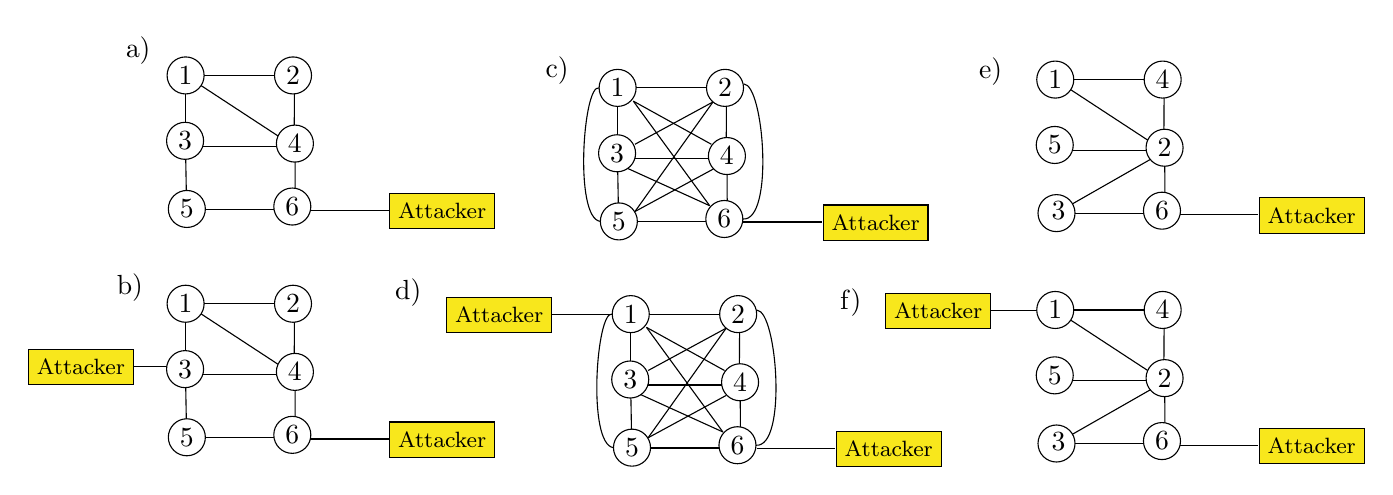
\begin{tikzpicture}[x=0.75pt,y=0.75pt,yscale=-1,xscale=1]
%uncomment if require: \path (0,300); %set diagram left start at 0, and has height of 300

%Straight Lines [id:da21270339539187544] 
\draw    (50.75,166.4) -- (88.67,166.4) ;


%Shape: Rectangle [id:dp19806528063640816] 
\draw  [fill={rgb, 255:red, 248; green, 231; blue, 28 }  ,fill opacity=1 ] (9.2,158.2) -- (59.67,158.2) -- (59.67,175.18) -- (9.2,175.18) -- cycle ;


%Straight Lines [id:da3153834125753151] 
\draw    (137.33,132.22) -- (137.17,163.81) ;


%Straight Lines [id:da7084115546458901] 
\draw    (91.08,200.73) -- (129,200.73) ;


%Straight Lines [id:da9623839826112595] 
\draw    (84.83,136.23) -- (140.58,172.73) ;


%Straight Lines [id:da2909368745777172] 
\draw    (84.83,172.73) -- (85.33,200.55) ;


%Straight Lines [id:da35867881660722734] 
\draw    (137.58,170.73) -- (137.67,202.88) ;


%Shape: Circle [id:dp9939759302306557] 
\draw  [fill={rgb, 255:red, 255; green, 255; blue, 255 }  ,fill opacity=1 ] (75.92,136.23) .. controls (75.92,131.3) and (79.91,127.31) .. (84.83,127.31) .. controls (89.76,127.31) and (93.75,131.3) .. (93.75,136.23) .. controls (93.75,141.15) and (89.76,145.15) .. (84.83,145.15) .. controls (79.91,145.15) and (75.92,141.15) .. (75.92,136.23) -- cycle ;

%Shape: Circle [id:dp34760301125310855] 
\draw  [fill={rgb, 255:red, 255; green, 255; blue, 255 }  ,fill opacity=1 ] (128.58,169.06) .. controls (128.58,164.14) and (132.58,160.15) .. (137.5,160.15) .. controls (142.42,160.15) and (146.42,164.14) .. (146.42,169.06) .. controls (146.42,173.99) and (142.42,177.98) .. (137.5,177.98) .. controls (132.58,177.98) and (128.58,173.99) .. (128.58,169.06) -- cycle ;

%Shape: Circle [id:dp9702116004071654] 
\draw  [fill={rgb, 255:red, 255; green, 255; blue, 255 }  ,fill opacity=1 ] (127.33,199.4) .. controls (127.33,194.47) and (131.33,190.48) .. (136.25,190.48) .. controls (141.17,190.48) and (145.17,194.47) .. (145.17,199.4) .. controls (145.17,204.32) and (141.17,208.31) .. (136.25,208.31) .. controls (131.33,208.31) and (127.33,204.32) .. (127.33,199.4) -- cycle ;

%Straight Lines [id:da8265544446705831] 
\draw    (93.75,136.23) -- (131.67,136.23) ;


%Straight Lines [id:da1435228669726185] 
\draw    (90.75,170.4) -- (128.67,170.4) ;


%Straight Lines [id:da5512583348761163] 
\draw    (84.83,145.15) -- (84.83,163.81) ;


%Shape: Circle [id:dp33954226442737345] 
\draw  [fill={rgb, 255:red, 255; green, 255; blue, 255 }  ,fill opacity=1 ] (76.52,200.56) .. controls (76.52,195.64) and (80.51,191.65) .. (85.43,191.65) .. controls (90.36,191.65) and (94.35,195.64) .. (94.35,200.56) .. controls (94.35,205.49) and (90.36,209.48) .. (85.43,209.48) .. controls (80.51,209.48) and (76.52,205.49) .. (76.52,200.56) -- cycle ;

%Shape: Circle [id:dp027045110799332694] 
\draw  [fill={rgb, 255:red, 255; green, 255; blue, 255 }  ,fill opacity=1 ] (75.67,167.73) .. controls (75.67,162.8) and (79.66,158.81) .. (84.58,158.81) .. controls (89.51,158.81) and (93.5,162.8) .. (93.5,167.73) .. controls (93.5,172.65) and (89.51,176.65) .. (84.58,176.65) .. controls (79.66,176.65) and (75.67,172.65) .. (75.67,167.73) -- cycle ;

%Shape: Circle [id:dp8622510797031577] 
\draw  [fill={rgb, 255:red, 255; green, 255; blue, 255 }  ,fill opacity=1 ] (127.67,136.23) .. controls (127.67,131.3) and (131.66,127.31) .. (136.58,127.31) .. controls (141.51,127.31) and (145.5,131.3) .. (145.5,136.23) .. controls (145.5,141.15) and (141.51,145.15) .. (136.58,145.15) .. controls (131.66,145.15) and (127.67,141.15) .. (127.67,136.23) -- cycle ;

%Straight Lines [id:da8162398929728556] 
\draw    (144.75,201.4) -- (182.67,201.4) ;


%Shape: Rectangle [id:dp15602990655598958] 
\draw  [fill={rgb, 255:red, 248; green, 231; blue, 28 }  ,fill opacity=1 ] (183.2,193.2) -- (233.67,193.2) -- (233.67,210.18) -- (183.2,210.18) -- cycle ;




%Straight Lines [id:da675337569741544] 
\draw    (137.33,22.22) -- (137.17,53.81) ;


%Straight Lines [id:da9770217193149313] 
\draw    (91.08,90.73) -- (129,90.73) ;


%Straight Lines [id:da18857026751215256] 
\draw    (84.83,26.23) -- (140.58,62.73) ;


%Straight Lines [id:da6275844068359788] 
\draw    (84.83,62.73) -- (85.33,90.55) ;


%Straight Lines [id:da3859409733288094] 
\draw    (137.58,60.73) -- (137.67,92.88) ;


%Shape: Circle [id:dp38555186789719464] 
\draw  [fill={rgb, 255:red, 255; green, 255; blue, 255 }  ,fill opacity=1 ] (75.92,26.23) .. controls (75.92,21.3) and (79.91,17.31) .. (84.83,17.31) .. controls (89.76,17.31) and (93.75,21.3) .. (93.75,26.23) .. controls (93.75,31.15) and (89.76,35.15) .. (84.83,35.15) .. controls (79.91,35.15) and (75.92,31.15) .. (75.92,26.23) -- cycle ;

%Shape: Circle [id:dp6614919206504822] 
\draw  [fill={rgb, 255:red, 255; green, 255; blue, 255 }  ,fill opacity=1 ] (128.58,59.06) .. controls (128.58,54.14) and (132.58,50.15) .. (137.5,50.15) .. controls (142.42,50.15) and (146.42,54.14) .. (146.42,59.06) .. controls (146.42,63.99) and (142.42,67.98) .. (137.5,67.98) .. controls (132.58,67.98) and (128.58,63.99) .. (128.58,59.06) -- cycle ;

%Shape: Circle [id:dp4792028510349877] 
\draw  [fill={rgb, 255:red, 255; green, 255; blue, 255 }  ,fill opacity=1 ] (127.33,89.4) .. controls (127.33,84.47) and (131.33,80.48) .. (136.25,80.48) .. controls (141.17,80.48) and (145.17,84.47) .. (145.17,89.4) .. controls (145.17,94.32) and (141.17,98.31) .. (136.25,98.31) .. controls (131.33,98.31) and (127.33,94.32) .. (127.33,89.4) -- cycle ;

%Straight Lines [id:da5503390690988923] 
\draw    (93.75,26.23) -- (131.67,26.23) ;


%Straight Lines [id:da4684291204598492] 
\draw    (90.75,60.4) -- (128.67,60.4) ;


%Straight Lines [id:da14625515615077633] 
\draw    (84.83,35.15) -- (84.83,53.81) ;


%Shape: Circle [id:dp5312971223005962] 
\draw  [fill={rgb, 255:red, 255; green, 255; blue, 255 }  ,fill opacity=1 ] (76.52,90.56) .. controls (76.52,85.64) and (80.51,81.65) .. (85.43,81.65) .. controls (90.36,81.65) and (94.35,85.64) .. (94.35,90.56) .. controls (94.35,95.49) and (90.36,99.48) .. (85.43,99.48) .. controls (80.51,99.48) and (76.52,95.49) .. (76.52,90.56) -- cycle ;

%Shape: Circle [id:dp8123330510491519] 
\draw  [fill={rgb, 255:red, 255; green, 255; blue, 255 }  ,fill opacity=1 ] (75.67,57.73) .. controls (75.67,52.8) and (79.66,48.81) .. (84.58,48.81) .. controls (89.51,48.81) and (93.5,52.8) .. (93.5,57.73) .. controls (93.5,62.65) and (89.51,66.65) .. (84.58,66.65) .. controls (79.66,66.65) and (75.67,62.65) .. (75.67,57.73) -- cycle ;

%Shape: Circle [id:dp008503760549775086] 
\draw  [fill={rgb, 255:red, 255; green, 255; blue, 255 }  ,fill opacity=1 ] (127.67,26.23) .. controls (127.67,21.3) and (131.66,17.31) .. (136.58,17.31) .. controls (141.51,17.31) and (145.5,21.3) .. (145.5,26.23) .. controls (145.5,31.15) and (141.51,35.15) .. (136.58,35.15) .. controls (131.66,35.15) and (127.67,31.15) .. (127.67,26.23) -- cycle ;

%Straight Lines [id:da5256421122460654] 
\draw    (144.75,91.4) -- (182.67,91.4) ;


%Shape: Rectangle [id:dp7797605979818211] 
\draw  [fill={rgb, 255:red, 248; green, 231; blue, 28 }  ,fill opacity=1 ] (183.2,83.2) -- (233.67,83.2) -- (233.67,100.18) -- (183.2,100.18) -- cycle ;




%Straight Lines [id:da22867619419553487] 
\draw    (345.47,28.22) -- (345.31,59.81) ;


%Straight Lines [id:da7366629057200433] 
\draw    (299.22,96.73) -- (337.14,96.73) ;


%Straight Lines [id:da5560609381608291] 
\draw    (292.97,68.73) -- (293.47,96.55) ;


%Straight Lines [id:da4739025620423759] 
\draw    (345.72,66.73) -- (345.81,98.88) ;


%Shape: Circle [id:dp9922005762933758] 
\draw  [fill={rgb, 255:red, 255; green, 255; blue, 255 }  ,fill opacity=1 ] (284.06,32.23) .. controls (284.06,27.3) and (288.05,23.31) .. (292.97,23.31) .. controls (297.9,23.31) and (301.89,27.3) .. (301.89,32.23) .. controls (301.89,37.15) and (297.9,41.15) .. (292.97,41.15) .. controls (288.05,41.15) and (284.06,37.15) .. (284.06,32.23) -- cycle ;

%Shape: Circle [id:dp7388325613342047] 
\draw  [fill={rgb, 255:red, 255; green, 255; blue, 255 }  ,fill opacity=1 ] (336.72,65.06) .. controls (336.72,60.14) and (340.72,56.15) .. (345.64,56.15) .. controls (350.57,56.15) and (354.56,60.14) .. (354.56,65.06) .. controls (354.56,69.99) and (350.57,73.98) .. (345.64,73.98) .. controls (340.72,73.98) and (336.72,69.99) .. (336.72,65.06) -- cycle ;

%Shape: Circle [id:dp3047262312307377] 
\draw  [fill={rgb, 255:red, 255; green, 255; blue, 255 }  ,fill opacity=1 ] (335.47,95.4) .. controls (335.47,90.47) and (339.47,86.48) .. (344.39,86.48) .. controls (349.32,86.48) and (353.31,90.47) .. (353.31,95.4) .. controls (353.31,100.32) and (349.32,104.31) .. (344.39,104.31) .. controls (339.47,104.31) and (335.47,100.32) .. (335.47,95.4) -- cycle ;

%Straight Lines [id:da5232789861595977] 
\draw    (301.89,32.23) -- (339.81,32.23) ;


%Straight Lines [id:da39641445777079876] 
\draw    (298.89,66.4) -- (336.81,66.4) ;


%Straight Lines [id:da6500529894480953] 
\draw    (292.97,41.15) -- (292.97,59.81) ;


%Shape: Circle [id:dp421295758241513] 
\draw  [fill={rgb, 255:red, 255; green, 255; blue, 255 }  ,fill opacity=1 ] (284.66,96.56) .. controls (284.66,91.64) and (288.65,87.65) .. (293.57,87.65) .. controls (298.5,87.65) and (302.49,91.64) .. (302.49,96.56) .. controls (302.49,101.49) and (298.5,105.48) .. (293.57,105.48) .. controls (288.65,105.48) and (284.66,101.49) .. (284.66,96.56) -- cycle ;

%Shape: Circle [id:dp68993621237352] 
\draw  [fill={rgb, 255:red, 255; green, 255; blue, 255 }  ,fill opacity=1 ] (283.81,63.73) .. controls (283.81,58.8) and (287.8,54.81) .. (292.72,54.81) .. controls (297.65,54.81) and (301.64,58.8) .. (301.64,63.73) .. controls (301.64,68.65) and (297.65,72.65) .. (292.72,72.65) .. controls (287.8,72.65) and (283.81,68.65) .. (283.81,63.73) -- cycle ;

%Shape: Circle [id:dp0004348717523896539] 
\draw  [fill={rgb, 255:red, 255; green, 255; blue, 255 }  ,fill opacity=1 ] (335.81,32.23) .. controls (335.81,27.3) and (339.8,23.31) .. (344.72,23.31) .. controls (349.65,23.31) and (353.64,27.3) .. (353.64,32.23) .. controls (353.64,37.15) and (349.65,41.15) .. (344.72,41.15) .. controls (339.8,41.15) and (335.81,37.15) .. (335.81,32.23) -- cycle ;

%Straight Lines [id:da3470843344836425] 
\draw    (297.74,71) -- (337.34,89) ;


%Straight Lines [id:da22385827339648745] 
\draw    (300.54,38.6) -- (338.14,59.4) ;


%Straight Lines [id:da9470627692324495] 
\draw    (301.34,59.4) -- (338.94,39) ;


%Straight Lines [id:da527163614428479] 
\draw    (301.34,91.8) -- (338.94,71.4) ;


%Curve Lines [id:da2659177622157741] 
\draw    (353.81,30.33) .. controls (363.47,30.67) and (368.47,96.67) .. (353.31,95.4) ;


%Curve Lines [id:da3968887523398855] 
\draw    (284.06,32.23) .. controls (276.47,30) and (271.81,95) .. (284.66,96.56) ;


%Straight Lines [id:da4862470624661749] 
\draw    (300.54,38.6) -- (337.34,89) ;


%Straight Lines [id:da9265421066580971] 
\draw    (338.94,39) -- (301.34,91.8) ;


%Straight Lines [id:da7131649869831252] 
\draw    (353.61,96.82) -- (391.52,96.82) ;


%Shape: Rectangle [id:dp3615803597823173] 
\draw  [fill={rgb, 255:red, 248; green, 231; blue, 28 }  ,fill opacity=1 ] (392.06,88.63) -- (442.53,88.63) -- (442.53,105.61) -- (392.06,105.61) -- cycle ;




%Straight Lines [id:da6715977826012206] 
\draw    (351.81,137.22) -- (351.64,168.81) ;


%Straight Lines [id:da9540657786576023] 
\draw    (305.56,205.73) -- (343.48,205.73) ;


%Straight Lines [id:da5731952874596753] 
\draw    (299.31,177.73) -- (299.81,205.55) ;


%Straight Lines [id:da41041637205710924] 
\draw    (352.06,175.73) -- (352.14,207.88) ;


%Shape: Circle [id:dp7490995910930758] 
\draw  [fill={rgb, 255:red, 255; green, 255; blue, 255 }  ,fill opacity=1 ] (290.39,141.23) .. controls (290.39,136.3) and (294.38,132.31) .. (299.31,132.31) .. controls (304.23,132.31) and (308.23,136.3) .. (308.23,141.23) .. controls (308.23,146.15) and (304.23,150.15) .. (299.31,150.15) .. controls (294.38,150.15) and (290.39,146.15) .. (290.39,141.23) -- cycle ;

%Shape: Circle [id:dp21867347242120194] 
\draw  [fill={rgb, 255:red, 255; green, 255; blue, 255 }  ,fill opacity=1 ] (343.06,174.06) .. controls (343.06,169.14) and (347.05,165.15) .. (351.98,165.15) .. controls (356.9,165.15) and (360.89,169.14) .. (360.89,174.06) .. controls (360.89,178.99) and (356.9,182.98) .. (351.98,182.98) .. controls (347.05,182.98) and (343.06,178.99) .. (343.06,174.06) -- cycle ;

%Shape: Circle [id:dp009688206133991684] 
\draw  [fill={rgb, 255:red, 255; green, 255; blue, 255 }  ,fill opacity=1 ] (341.81,204.4) .. controls (341.81,199.47) and (345.8,195.48) .. (350.73,195.48) .. controls (355.65,195.48) and (359.64,199.47) .. (359.64,204.4) .. controls (359.64,209.32) and (355.65,213.31) .. (350.73,213.31) .. controls (345.8,213.31) and (341.81,209.32) .. (341.81,204.4) -- cycle ;

%Straight Lines [id:da45622560516359056] 
\draw    (308.23,141.23) -- (346.14,141.23) ;


%Straight Lines [id:da8381919416870578] 
\draw    (305.23,175.4) -- (343.14,175.4) ;


%Straight Lines [id:da6163529535308253] 
\draw    (299.31,150.15) -- (299.31,168.81) ;


%Shape: Circle [id:dp456728946120202] 
\draw  [fill={rgb, 255:red, 255; green, 255; blue, 255 }  ,fill opacity=1 ] (290.99,205.56) .. controls (290.99,200.64) and (294.98,196.65) .. (299.91,196.65) .. controls (304.83,196.65) and (308.83,200.64) .. (308.83,205.56) .. controls (308.83,210.49) and (304.83,214.48) .. (299.91,214.48) .. controls (294.98,214.48) and (290.99,210.49) .. (290.99,205.56) -- cycle ;

%Shape: Circle [id:dp45682398029629745] 
\draw  [fill={rgb, 255:red, 255; green, 255; blue, 255 }  ,fill opacity=1 ] (290.14,172.73) .. controls (290.14,167.8) and (294.13,163.81) .. (299.06,163.81) .. controls (303.98,163.81) and (307.98,167.8) .. (307.98,172.73) .. controls (307.98,177.65) and (303.98,181.65) .. (299.06,181.65) .. controls (294.13,181.65) and (290.14,177.65) .. (290.14,172.73) -- cycle ;

%Shape: Circle [id:dp20828836021634367] 
\draw  [fill={rgb, 255:red, 255; green, 255; blue, 255 }  ,fill opacity=1 ] (342.14,141.23) .. controls (342.14,136.3) and (346.13,132.31) .. (351.06,132.31) .. controls (355.98,132.31) and (359.98,136.3) .. (359.98,141.23) .. controls (359.98,146.15) and (355.98,150.15) .. (351.06,150.15) .. controls (346.13,150.15) and (342.14,146.15) .. (342.14,141.23) -- cycle ;

%Straight Lines [id:da32117265204513157] 
\draw    (304.08,180) -- (343.68,198) ;


%Straight Lines [id:da6079841314173954] 
\draw    (306.88,147.6) -- (344.48,168.4) ;


%Straight Lines [id:da7680118845457601] 
\draw    (307.68,168.4) -- (345.28,148) ;


%Straight Lines [id:da6389773826545454] 
\draw    (307.68,200.8) -- (345.28,180.4) ;


%Curve Lines [id:da511824766847756] 
\draw    (360.14,139.33) .. controls (369.81,139.67) and (374.81,205.67) .. (359.64,204.4) ;


%Curve Lines [id:da10840460492754567] 
\draw    (290.39,141.23) .. controls (282.81,139) and (278.14,204) .. (290.99,205.56) ;


%Straight Lines [id:da3147720372519749] 
\draw    (306.88,147.6) -- (343.68,198) ;


%Straight Lines [id:da9757233447370841] 
\draw    (345.28,148) -- (307.68,200.8) ;


%Straight Lines [id:da8351826345519837] 
\draw    (359.94,205.82) -- (397.86,205.82) ;


%Shape: Rectangle [id:dp9492523154356004] 
\draw  [fill={rgb, 255:red, 248; green, 231; blue, 28 }  ,fill opacity=1 ] (398.39,197.63) -- (448.86,197.63) -- (448.86,214.61) -- (398.39,214.61) -- cycle ;


%Straight Lines [id:da7783875840754805] 
\draw    (252.23,141.4) -- (290.14,141.4) ;


%Shape: Rectangle [id:dp8219665960733671] 
\draw  [fill={rgb, 255:red, 248; green, 231; blue, 28 }  ,fill opacity=1 ] (210.68,133.2) -- (261.15,133.2) -- (261.15,150.18) -- (210.68,150.18) -- cycle ;



%Straight Lines [id:da7147269629924605] 
\draw    (556.33,24.22) -- (556.17,55.81) ;


%Straight Lines [id:da8277651830187894] 
\draw    (510.08,92.73) -- (548,92.73) ;


%Straight Lines [id:da0013601110130750937] 
\draw    (503.83,28.23) -- (559.58,64.73) ;


%Straight Lines [id:da5364857137309426] 
\draw    (556.58,62.73) -- (504.33,92.55) ;


%Straight Lines [id:da09227991689524317] 
\draw    (556.58,62.73) -- (556.67,94.88) ;


%Shape: Circle [id:dp40945899905332894] 
\draw  [fill={rgb, 255:red, 255; green, 255; blue, 255 }  ,fill opacity=1 ] (494.92,28.23) .. controls (494.92,23.3) and (498.91,19.31) .. (503.83,19.31) .. controls (508.76,19.31) and (512.75,23.3) .. (512.75,28.23) .. controls (512.75,33.15) and (508.76,37.15) .. (503.83,37.15) .. controls (498.91,37.15) and (494.92,33.15) .. (494.92,28.23) -- cycle ;

%Shape: Circle [id:dp7767184939243962] 
\draw  [fill={rgb, 255:red, 255; green, 255; blue, 255 }  ,fill opacity=1 ] (547.58,61.06) .. controls (547.58,56.14) and (551.58,52.15) .. (556.5,52.15) .. controls (561.42,52.15) and (565.42,56.14) .. (565.42,61.06) .. controls (565.42,65.99) and (561.42,69.98) .. (556.5,69.98) .. controls (551.58,69.98) and (547.58,65.99) .. (547.58,61.06) -- cycle ;
%Shape: Circle [id:dp4692699516703288] 
\draw  [fill={rgb, 255:red, 255; green, 255; blue, 255 }  ,fill opacity=1 ] (546.33,91.4) .. controls (546.33,86.47) and (550.33,82.48) .. (555.25,82.48) .. controls (560.17,82.48) and (564.17,86.47) .. (564.17,91.4) .. controls (564.17,96.32) and (560.17,100.31) .. (555.25,100.31) .. controls (550.33,100.31) and (546.33,96.32) .. (546.33,91.4) -- cycle ;

%Straight Lines [id:da9597316941694047] 
\draw    (512.75,28.23) -- (550.67,28.23) ;


%Straight Lines [id:da7708545450116795] 
\draw    (509.75,62.4) -- (547.67,62.4) ;


%Shape: Circle [id:dp40660215241265885] 
\draw  [fill={rgb, 255:red, 255; green, 255; blue, 255 }  ,fill opacity=1 ] (495.52,92.56) .. controls (495.52,87.64) and (499.51,83.65) .. (504.43,83.65) .. controls (509.36,83.65) and (513.35,87.64) .. (513.35,92.56) .. controls (513.35,97.49) and (509.36,101.48) .. (504.43,101.48) .. controls (499.51,101.48) and (495.52,97.49) .. (495.52,92.56) -- cycle ;
%Shape: Circle [id:dp09457558597010363] 
\draw  [fill={rgb, 255:red, 255; green, 255; blue, 255 }  ,fill opacity=1 ] (494.67,59.73) .. controls (494.67,54.8) and (498.66,50.81) .. (503.58,50.81) .. controls (508.51,50.81) and (512.5,54.8) .. (512.5,59.73) .. controls (512.5,64.65) and (508.51,68.65) .. (503.58,68.65) .. controls (498.66,68.65) and (494.67,64.65) .. (494.67,59.73) -- cycle ;
%Shape: Circle [id:dp7445040256787864] 
\draw  [fill={rgb, 255:red, 255; green, 255; blue, 255 }  ,fill opacity=1 ] (546.67,28.23) .. controls (546.67,23.3) and (550.66,19.31) .. (555.58,19.31) .. controls (560.51,19.31) and (564.5,23.3) .. (564.5,28.23) .. controls (564.5,33.15) and (560.51,37.15) .. (555.58,37.15) .. controls (550.66,37.15) and (546.67,33.15) .. (546.67,28.23) -- cycle ;
%Straight Lines [id:da6980179493369204] 
\draw    (563.75,93.4) -- (601.67,93.4) ;


%Shape: Rectangle [id:dp9981691173299058] 
\draw  [fill={rgb, 255:red, 248; green, 231; blue, 28 }  ,fill opacity=1 ] (602.2,85.2) -- (652.67,85.2) -- (652.67,102.18) -- (602.2,102.18) -- cycle ;




%Straight Lines [id:da8092387671610324] 
\draw    (463.75,139.4) -- (501.67,139.4) ;


%Shape: Rectangle [id:dp7958055249044546] 
\draw  [fill={rgb, 255:red, 248; green, 231; blue, 28 }  ,fill opacity=1 ] (422.2,131.2) -- (472.67,131.2) -- (472.67,148.18) -- (422.2,148.18) -- cycle ;


%Straight Lines [id:da8513354272469744] 
\draw    (556.33,135.22) -- (556.17,166.81) ;


%Straight Lines [id:da7992137672953211] 
\draw    (510.08,203.73) -- (548,203.73) ;


%Straight Lines [id:da3954660742507915] 
\draw    (503.83,139.23) -- (559.58,175.73) ;


%Straight Lines [id:da5825560768425334] 
\draw    (556.58,173.73) -- (504.33,203.55) ;


%Straight Lines [id:da5568053188323774] 
\draw    (556.58,173.73) -- (556.67,205.88) ;


%Shape: Circle [id:dp30253748945575554] 
\draw  [fill={rgb, 255:red, 255; green, 255; blue, 255 }  ,fill opacity=1 ] (494.92,139.23) .. controls (494.92,134.3) and (498.91,130.31) .. (503.83,130.31) .. controls (508.76,130.31) and (512.75,134.3) .. (512.75,139.23) .. controls (512.75,144.15) and (508.76,148.15) .. (503.83,148.15) .. controls (498.91,148.15) and (494.92,144.15) .. (494.92,139.23) -- cycle ;

%Shape: Circle [id:dp3641428183407782] 
\draw  [fill={rgb, 255:red, 255; green, 255; blue, 255 }  ,fill opacity=1 ] (547.58,172.06) .. controls (547.58,167.14) and (551.58,163.15) .. (556.5,163.15) .. controls (561.42,163.15) and (565.42,167.14) .. (565.42,172.06) .. controls (565.42,176.99) and (561.42,180.98) .. (556.5,180.98) .. controls (551.58,180.98) and (547.58,176.99) .. (547.58,172.06) -- cycle ;
%Shape: Circle [id:dp08738614749957285] 
\draw  [fill={rgb, 255:red, 255; green, 255; blue, 255 }  ,fill opacity=1 ] (546.33,202.4) .. controls (546.33,197.47) and (550.33,193.48) .. (555.25,193.48) .. controls (560.17,193.48) and (564.17,197.47) .. (564.17,202.4) .. controls (564.17,207.32) and (560.17,211.31) .. (555.25,211.31) .. controls (550.33,211.31) and (546.33,207.32) .. (546.33,202.4) -- cycle ;

%Straight Lines [id:da8382293979078496] 
\draw    (512.75,139.23) -- (550.67,139.23) ;


%Straight Lines [id:da06888701209203096] 
\draw    (509.75,173.4) -- (547.67,173.4) ;


%Shape: Circle [id:dp03475136247746857] 
\draw  [fill={rgb, 255:red, 255; green, 255; blue, 255 }  ,fill opacity=1 ] (495.52,203.56) .. controls (495.52,198.64) and (499.51,194.65) .. (504.43,194.65) .. controls (509.36,194.65) and (513.35,198.64) .. (513.35,203.56) .. controls (513.35,208.49) and (509.36,212.48) .. (504.43,212.48) .. controls (499.51,212.48) and (495.52,208.49) .. (495.52,203.56) -- cycle ;
%Shape: Circle [id:dp825936328113765] 
\draw  [fill={rgb, 255:red, 255; green, 255; blue, 255 }  ,fill opacity=1 ] (494.67,170.73) .. controls (494.67,165.8) and (498.66,161.81) .. (503.58,161.81) .. controls (508.51,161.81) and (512.5,165.8) .. (512.5,170.73) .. controls (512.5,175.65) and (508.51,179.65) .. (503.58,179.65) .. controls (498.66,179.65) and (494.67,175.65) .. (494.67,170.73) -- cycle ;
%Shape: Circle [id:dp10791744420385518] 
\draw  [fill={rgb, 255:red, 255; green, 255; blue, 255 }  ,fill opacity=1 ] (546.67,139.23) .. controls (546.67,134.3) and (550.66,130.31) .. (555.58,130.31) .. controls (560.51,130.31) and (564.5,134.3) .. (564.5,139.23) .. controls (564.5,144.15) and (560.51,148.15) .. (555.58,148.15) .. controls (550.66,148.15) and (546.67,144.15) .. (546.67,139.23) -- cycle ;
%Straight Lines [id:da35173459455787404] 
\draw    (563.75,204.4) -- (601.67,204.4) ;


%Shape: Rectangle [id:dp6910000106247179] 
\draw  [fill={rgb, 255:red, 248; green, 231; blue, 28 }  ,fill opacity=1 ] (602.2,196.2) -- (652.67,196.2) -- (652.67,213.18) -- (602.2,213.18) -- cycle ;




% Text Node
\draw (405.33,135.67) node  [align=left] {f)};
% Text Node
\draw (556.5,172.06) node  [align=left] {2};
% Text Node
\draw (505.43,202.56) node  [align=left] {3};
% Text Node
\draw (503.58,170.73) node  [align=left] {5};
% Text Node
\draw (555.58,139.23) node  [align=left] {4};
% Text Node
\draw (627.44,204.69) node  [align=left] {{\footnotesize Attacker}};
% Text Node
\draw (555.25,202.4) node  [align=left] {6};
% Text Node
\draw (503.83,139.23) node  [align=left] {1};
% Text Node
\draw (447.44,139.69) node  [align=left] {{\footnotesize Attacker}};
% Text Node
\draw (472.67,24.33) node  [align=left] {e)};
% Text Node
\draw (556.5,61.06) node  [align=left] {2};
% Text Node
\draw (505.43,91.56) node  [align=left] {3};
% Text Node
\draw (503.58,59.73) node  [align=left] {5};
% Text Node
\draw (555.58,28.23) node  [align=left] {4};
% Text Node
\draw (627.44,93.69) node  [align=left] {{\footnotesize Attacker}};
% Text Node
\draw (555.25,91.4) node  [align=left] {6};
% Text Node
\draw (503.83,28.23) node  [align=left] {1};
% Text Node
\draw (192.14,131) node  [align=left] {d)};
% Text Node
\draw (235.91,141.69) node  [align=left] {{\footnotesize Attacker}};
% Text Node
\draw (423.63,206.12) node  [align=left] {{\footnotesize Attacker}};
% Text Node
\draw (351.06,141.23) node  [align=left] {2};
% Text Node
\draw (299.06,172.73) node  [align=left] {3};
% Text Node
\draw (299.91,205.56) node  [align=left] {5};
% Text Node
\draw (350.73,204.4) node  [align=left] {6};
% Text Node
\draw (351.98,174.06) node  [align=left] {4};
% Text Node
\draw (299.31,141.23) node  [align=left] {1};
% Text Node
\draw (263.81,24) node  [align=left] {c)};
% Text Node
\draw (417.29,97.12) node  [align=left] {{\footnotesize Attacker}};
% Text Node
\draw (344.72,32.23) node  [align=left] {2};
% Text Node
\draw (292.72,63.73) node  [align=left] {3};
% Text Node
\draw (293.57,96.56) node  [align=left] {5};
% Text Node
\draw (344.39,95.4) node  [align=left] {6};
% Text Node
\draw (345.64,65.06) node  [align=left] {4};
% Text Node
\draw (292.97,32.23) node  [align=left] {1};
% Text Node
\draw (62,14.33) node  [align=left] {a)};
% Text Node
\draw (208.44,91.69) node  [align=left] {{\footnotesize Attacker}};
% Text Node
\draw (136.58,26.23) node  [align=left] {2};
% Text Node
\draw (84.58,57.73) node  [align=left] {3};
% Text Node
\draw (85.43,90.56) node  [align=left] {5};
% Text Node
\draw (136.25,89.4) node  [align=left] {6};
% Text Node
\draw (137.5,59.06) node  [align=left] {4};
% Text Node
\draw (84.83,26.23) node  [align=left] {1};
% Text Node
\draw (58,128.33) node  [align=left] {b)};
% Text Node
\draw (208.44,201.69) node  [align=left] {{\footnotesize Attacker}};
% Text Node
\draw (136.58,136.23) node  [align=left] {2};
% Text Node
\draw (84.58,167.73) node  [align=left] {3};
% Text Node
\draw (85.43,200.56) node  [align=left] {5};
% Text Node
\draw (136.25,199.4) node  [align=left] {6};
% Text Node
\draw (137.5,169.06) node  [align=left] {4};
% Text Node
\draw (84.83,136.23) node  [align=left] {1};
% Text Node
\draw (34.44,166.69) node  [align=left] {{\footnotesize Attacker}};


\end{tikzpicture}


\caption{Use case topologies}
\label{fig:mdp-usecase-single}
\end{figure}

We run the MDP using different budgets and detection probabilities.
Nodes are migrated in the following order: 1, 2 and 3.
The ordering of the nodes impacts the result sets of Algorithm~\ref{algo:target}, thus which nodes may be attacked at each transition.
We have extracted the monitoring set of each absorbing state, and evaluated the overall reward of each monitoring set.
We define the reward of a monitoring set as the expected value of the reward of each corresponding absorbing state.
The expected value uses the stationary distribution of the Markov Chain corresponding to the optimal policy.
Details about the source node for attacks again the migration is summarized in Table~\ref{tab:mdp-attack-source}.

% Please add the following required packages to your document preamble:
% \usepackage{graphicx}
\begin{table}[h]
\resizebox{\textwidth}{!}{%
\begin{tabular}{|c|c|c|c|c|c|c|c|c|c|c|c|c|c|c|c|c|c|c|c|c|c|c|}
\cline{1-7} \cline{9-15} \cline{17-23}
\multicolumn{7}{|c|}{\textbf{Scenario b)}} &  & \multicolumn{7}{c|}{\textbf{Scenario d)}} &  & \multicolumn{7}{c|}{\textbf{Scenario f)}} \\ \cline{1-7} \cline{9-15} \cline{17-23} 
Target node    & 1  & 2  & 3  & 4  & 5 & 6 &  & Target node    & 1  & 2  & 3  & 4 & 5 & 6 &  & Target node    & 1  & 2  & 3  & 4 & 5 & 6 \\ \cline{1-7} \cline{9-15} \cline{17-23} 
Attack source  & 6  & 4  & 6  & 4  & 6 & 6 &  & Attack Source  & 6  & 6  & 1  & 6 & 1 & 1 &  & Attack source  & 6  & 6  & 1  & 6 & 1 & 1 \\ \cline{1-7} \cline{9-15} \cline{17-23} 
\end{tabular}%
}
\caption{Attack sources for multiple attackers scenarios}
\label{tab:mdp-attack-source}
\end{table}

\textbf{Scenario a) and b)\\}
Based on the paths taken by attacks and the ordering of the migration, we categorize the nodes into three categories: source, intermediate and border nodes. Source nodes are the origins of attacks, intermediate nodes are going to be on the path of attacks targeting the border nodes. 
The results are shown in Fig.~\ref{fig:mdp-result-topo1}.
The scenario a) sets the source to node 6, nodes 4 and 5 as intermediate nodes and finally nodes 1,2 and 3 as border nodes.
The scenario b) sets the source to nodes 3 and 6, nodes 1,4 as intermediate and nodes 2 and 5 as border nodes.
The first observation is that node 6 is globally the most rewarding node in both cases.
This is explained as it is the source of most of the attacks, and the exfiltrated data is redirected there.
In both scenarios the importance of nodes is separated according to the our categorization. 
This means that the nodes pertaining to the majority of attack paths are the most rewarded.
This is observation is reinforced in scenario b) where nodes 4 and 5 are close to attack sources while nodes 1 and 2 are further away.

In both scenarios, the detection rate does not have a significant impact on the ranking of the nodes, compared to each other.
In scenario a) results are stable from $p=0.6$ where node 6 overcomes node 4 in reward until $p=0.9$. All other nodes remain closely grouped, and no intermediate or border nodes is standing out.
In scenario b) the higher the detection rate the higher the reward of node 3, the second source of attacks.
The steadiness in the evolution of each node shows that the performance of the detection is not a major factor in determining which nodes are best suited for the monitoring. We formulate some hypotheses in Section~\ref{sec:mdp-discussion}.

Detailed examination of the optimal policy for each budget also shows that the monitoring action is rarely used to redeploy resource elsewhere in the infrastructure.
Instead of unmonitoring nodes, the MDP chooses to do nothing to preserve the global detection probability.
$m_j$ actions are only chosen when the unmonitored node does not detect the next attack, thus having the same impact as action $d$. These corner cases only represent a small percentage of the global solution where very few attacks occurred.

\textbf{Scenarios c) and d) \\}
In these scenarios, the topology considered is fullmeshed, which means that each physical node is connected to every other node of the infrastructure. This topology has been chosen to minimize the impact of the routing on the detection path because the attacker is always connected to the target node.
Results are shown in Fig.~\ref{fig:mdp-result-fullmesh}.

The first observation we make is that whether there is one or several attackers, the position of nodes between each other remains unchanged. This reinforce our conclusion that the routing of attacks has a real impact on the detection performance of each node.
The second observation we make is that the most important nodes are the main source of attacks as well as the first node being migrated. While the first node is an obvious choice for attack detection, the second shows another aspect of the model which is target selection. Indeed, since node 1 is always migrated first, it is therefore the main target at the first transition of the MDP.

% Finally, we have examined the different optimal policies for these scenarios, and observed that some corner cases have appeared.
Overall, the fact that for each attack only the origin of the attack and the target node may contribute to the detection has generated a diverse solution state. Indeed, depending on which node would be targeted there is a unique solution set to detect the attack and the fullmesh aspect of the topology makes it hard for those solution sets to overlap and give a better coverage.

\textbf{Scenarios e) and f) \\}

Using the same categorization as scenarios a) and b), we consider node 6 as a source node, node 2 as an intermediate node and nodes 1,3,4,5 as border nodes. Scenario f) transfers node 1 from a border node to a source node. Results are shown in Fig.~\ref{fig:mdp-result-topo2}.

In scenario e), the importance of each node depicted in Fig.~\ref{fig:mdp-result-topo2} reflect their role. Nodes 1,3,4 and 5 do not have much impact in the solution set, as they are not on the path of most of attacks. The attack source is still considered important to monitor and node 2 which acts as a ``bridge" between the two halves of the topology will belong to the path of a lot of attacks.

Scenario f) highlights similar results. There are now two attack sources, nodes 1 and 6. Moreover, the geographical distribution of migrated nodes gives more importance to node 2 which becomes even more present on the attack paths, as shown in Table~\ref{tab:mdp-attack-source}. This scenario is also the only one in which the main source of attacks is not consistently the most important node for the monitoring.

% Optimal policies also have some corner cases with counter intuitive optimal monitoring nodes but those remain marginal considering the solution space. 



\begin{figure}
    \centering
    \captionsetup[subfigure]{labelformat=empty}
\begin{subfigure}{.5\textwidth}
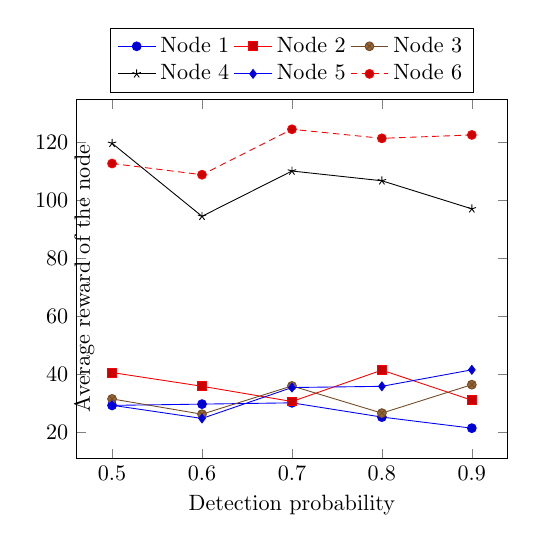
\begin{tikzpicture}[scale=0.8]
\begin{axis}[
  xlabel={Detection probability},
  ylabel={Average reward of the node },
  y label style={at={(0.06,0.5)}},
  xtick={0.5,0.6,0.7,0.8,0.9,1.0},
  legend style={at={(0.5,1.2)},cells={align=right}, anchor=north,legend columns=3},
  grid style=dashed,
]

\addplot+[]
    coordinates {
(0.5,29.2207587022)(0.6,29.6591500811)(0.7,30.107769581)(0.8,25.1808225374)(0.9,21.3501334315)
};

\addplot+[]
    coordinates {
(0.5,40.5649596864)(0.6,35.8317201966)(0.7,30.5615817425)(0.8,41.4017616625)(0.9,31.0018428294)
};

\addplot+[]
    coordinates {
(0.5,31.4601711216)(0.6,26.1715912622)(0.7,35.9427616495)(0.8,26.5488358659)(0.9,36.3780765072)
};

\addplot+[]
    coordinates {
(0.5,119.788927983)(0.6,94.566243579)(0.7,110.212449824)(0.8,106.844518821)(0.9,97.138069126)
};

\addplot+[]
    coordinates {
(0.5,29.2697135288)(0.6,24.7098561839)(0.7,35.3909999115)(0.8,35.8083893589)(0.9,41.5087141375)
};

\addplot+[]
    coordinates {
(0.5,112.808511307)(0.6,108.932780706)(0.7,124.631408718)(0.8,121.507931814)(0.9,122.678991306)
};

\legend{Node 1, Node 2, Node 3, Node 4, Node 5, Node 6}
\end{axis}
\end{tikzpicture}

\caption{Scenario a)}
\label{fig:nodeimp_single}
\end{subfigure}
\begin{subfigure}{.33\textwidth}
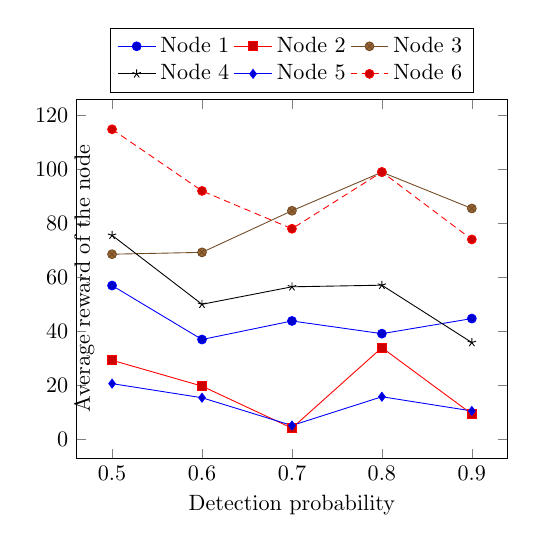
\begin{tikzpicture}[scale=0.8]
\begin{axis}[
  xlabel={Detection probability},
  ylabel={Average reward of the node },
  y label style={at={(0.06,0.5)}},
  xtick={0.5,0.6,0.7,0.8,0.9,1.0},
  legend style={at={(0.5,1.2)},cells={align=right}, anchor=north,legend columns=3},
  grid style=dashed,
]

\addplot+[]
    coordinates {
(0.5,57.0711574474)(0.6,37.0782125822)(0.7,43.9471043804)(0.8,39.2446371458)(0.9,44.8363801675)
};

\addplot+[]
    coordinates {
(0.5,29.4097815394)(0.6,19.8278112984)(0.7,4.26428571429)(0.8,34.0706693208)(0.9,9.49928571429)
};

\addplot+[]
    coordinates {
(0.5,68.6596096998)(0.6,69.339332514)(0.7,84.7438538657)(0.8,99.0264041517)(0.9,85.5894326243)
};

\addplot+[]
    coordinates {
(0.5,75.6609039908)(0.6,50.1243516403)(0.7,56.5923700845)(0.8,57.1874277411)(0.9,35.9649500717)
};

\addplot+[]
    coordinates {
(0.5,20.7573450249)(0.6,15.5267400966)(0.7,5.25375523139)(0.8,15.8992854434)(0.9,10.6415647894)
};

\addplot+[]
    coordinates {
(0.5,114.89762846)(0.6,92.0949728442)(0.7,78.0795310037)(0.8,99.102629324)(0.9,74.1266846482)
};

\legend{Node 1, Node 2, Node 3, Node 4, Node 5, Node 6}
\end{axis}
\end{tikzpicture}

\caption{Scenario b)}
\label{fig:nodeimp_topo1_multiple}
\end{subfigure}
    \caption{Results for single and multiple attackers}
    \label{fig:mdp-result-topo1}
\end{figure}
\begin{figure}
    \centering
    \captionsetup[subfigure]{labelformat=empty}
\begin{subfigure}{.5\textwidth}
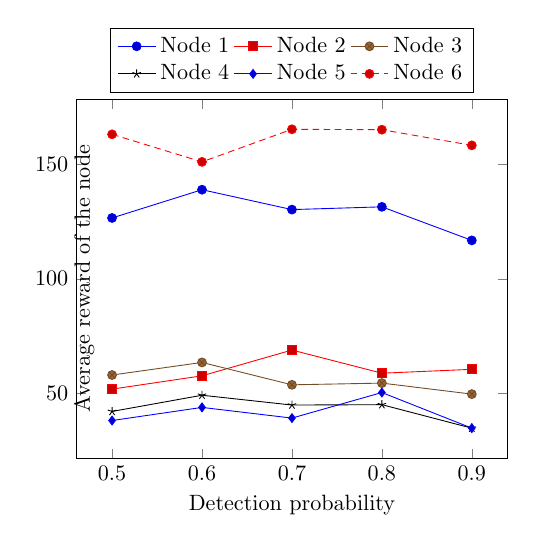
\begin{tikzpicture}[scale=0.8]
\begin{axis}[
  xlabel={Detection probability},
  ylabel={Average reward of the node },
  y label style={at={(0.06,0.5)}},
  xtick={0.5,0.6,0.7,0.8,0.9,1.0},
  legend style={at={(0.5,1.2)},cells={align=right}, anchor=north,legend columns=3},
  grid style=dashed,
]

\addplot+[]
    coordinates {
(0.5,126.469294224)(0.6,138.768688772)(0.7,130.10979383)(0.8,131.308647284)(0.9,116.70873472)
};

\addplot+[]
    coordinates {
(0.5,51.9774584454)(0.6,57.7615872131)(0.7,68.9811633084)(0.8,58.9060250618)(0.9,60.5911805552)
};

\addplot+[]
    coordinates {
(0.5,58.112876005)(0.6,63.5894390224)(0.7,53.8483204974)(0.8,54.5969922461)(0.9,49.8027670671)
};

\addplot+[]
    coordinates {
(0.5,42.2594496478)(0.6,49.3133895991)(0.7,45.0502147208)(0.8,45.20918204)(0.9,34.9808016775)
};

\addplot+[]
    coordinates {
(0.5,38.3055097066)(0.6,44.0188235767)(0.7,39.3680288222)(0.8,50.4912779668)(0.9,34.9978557067)
};

\addplot+[]
    coordinates {
(0.5,162.87848727)(0.6,150.876767477)(0.7,165.06110317)(0.8,164.882126918)(0.9,158.067481047)
};

\legend{Node 1, Node 2, Node 3, Node 4, Node 5, Node 6}
\end{axis}
\end{tikzpicture}

\caption{Scenario c)}
\label{fig:nodeimp_topofullmesh_single}
\end{subfigure}
\begin{subfigure}{.33\textwidth}
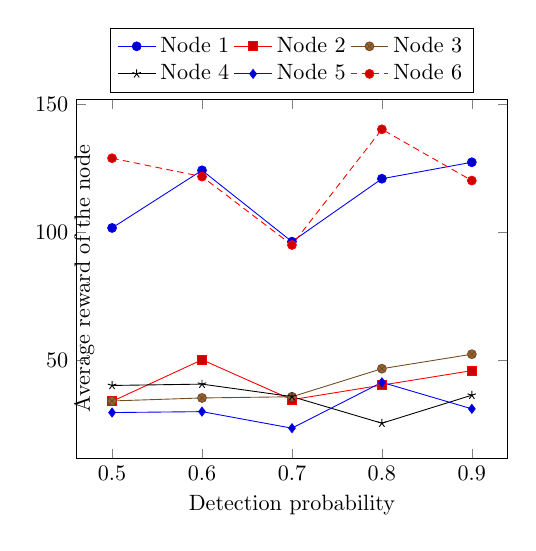
\begin{tikzpicture}[scale=0.8]
\begin{axis}[
  xlabel={Detection probability},
  ylabel={Average reward of the node },
  y label style={at={(0.06,0.5)}},
  xtick={0.5,0.6,0.7,0.8,0.9,1.0},
  legend style={at={(0.5,1.2)},cells={align=right}, anchor=north,legend columns=3},
  grid style=dashed,
]
\addplot+[]
    coordinates {
(0.5,101.616873023)(0.6,124.145242333)(0.7,96.2616914651)(0.8,120.862819291)(0.9,127.305784272)
};

\addplot+[]
    coordinates {
(0.5,33.8037034841)(0.6,50.0693289402)(0.7,34.460597311)(0.8,40.1535742549)(0.9,45.8166364524)
};

\addplot+[]
    coordinates {
(0.5,33.9581528218)(0.6,35.1326808601)(0.7,35.6074089582)(0.8,46.5769811834)(0.9,52.2400544067)
};

\addplot+[]
    coordinates {
(0.5,40.0224063598)(0.6,40.5434953331)(0.7,35.6681036149)(0.8,25.2556265302)(0.9,36.2111392677)
};

\addplot+[]
    coordinates {
(0.5,29.4251886633)(0.6,29.7859232959)(0.7,23.3183642626)(0.8,41.2471235042)(0.9,30.8838558151)
};

\addplot+[]
    coordinates {
(0.5,128.882560148)(0.6,121.704109507)(0.7,94.9489538016)(0.8,140.19719198)(0.9,120.142225907)
};


\legend{Node 1, Node 2, Node 3, Node 4, Node 5, Node 6}
\end{axis}
\end{tikzpicture}

\caption{Scenario d)}
\label{fig:nodeimp_topofullmesh_multiple}
\end{subfigure}
\caption{Results for single and multiple attackers - Scenarios c) and d)}
    \label{fig:mdp-result-fullmesh}
\end{figure}
\begin{figure}
    \centering
    \captionsetup[subfigure]{labelformat=empty}
\begin{subfigure}{.5\textwidth}
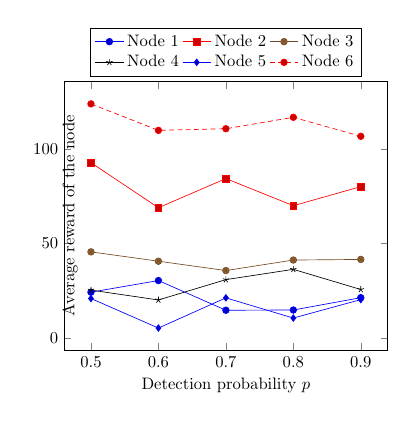
\begin{tikzpicture}[scale=0.6]
\begin{axis}[
  xlabel={Detection probability $p$},
  ylabel={Average reward of the node },
  y label style={at={(0.06,0.5)}},
  xtick={0.5,0.6,0.7,0.8,0.9,1.0},
  legend style={at={(0.5,1.2)},cells={align=right}, anchor=north,legend columns=3},
  grid style=dashed,
]
\addplot+[]
    coordinates {
(0.5,24.2596903238)(0.6,30.4098004181)(0.7,14.7157392372)(0.8,14.8410159329)(0.9,21.3512325325)
};

\addplot+[]
    coordinates {
(0.5,92.6967638225)(0.6,68.892572501)(0.7,84.3050837463)(0.8,69.9668923619)(0.9,80.051680541)
};

\addplot+[]
    coordinates {
(0.5,45.5695982478)(0.6,40.6246377658)(0.7,35.692885081)(0.8,41.2436256503)(0.9,41.5670235599)
};

\addplot+[]
    coordinates {
(0.5,25.3670893308)(0.6,20.1438895136)(0.7,30.888009803)(0.8,36.3312849347)(0.9,25.6728772368)
};

\addplot+[]
    coordinates {
(0.5,20.9174008986)(0.6,5.30161144168)(0.7,21.2602459651)(0.8,10.5837610733)(0.9,20.3331330431)
};

\addplot+[]
    coordinates {
(0.5,123.776293271)(0.6,109.788318837)(0.7,110.653974948)(0.8,116.685625909)(0.9,106.649803871)
};

\legend{Node 1, Node 2, Node 3, Node 4, Node 5, Node 6}
\end{axis}
\end{tikzpicture}

\caption{Scenario e)}
\label{fig:nodeimp_topo2_single}
\end{subfigure}
\begin{subfigure}{.33\textwidth}
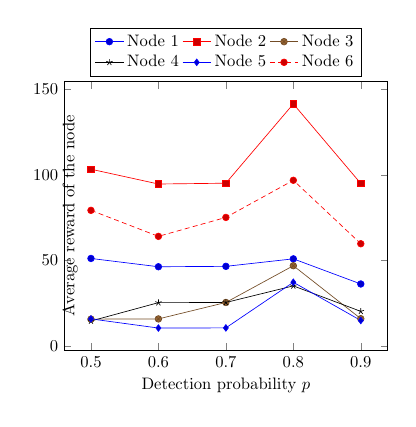
\begin{tikzpicture}[scale=0.6]
\begin{axis}[
  xlabel={Detection probability $p$},
  ylabel={Average reward of the node },
  y label style={at={(0.06,0.5)}},
  xtick={0.5,0.6,0.7,0.8,0.9,1.0},
  legend style={at={(0.5,1.2)},cells={align=right}, anchor=north,legend columns=3},
  grid style=dashed,
]

\addplot+[]
    coordinates {
(0.5,51.2408756424)(0.6,46.3989088055)(0.7,46.629281859)(0.8,51.0165854846)(0.9,36.3262102772)
};

\addplot+[]
    coordinates {
(0.5,103.390154828)(0.6,94.7445634867)(0.7,95.2136135648)(0.8,141.564157095)(0.9,95.0544799628)
};

\addplot+[]
    coordinates {
(0.5,15.7876437463)(0.6,15.9058652472)(0.7,25.5235856726)(0.8,47.0026051031)(0.9,16.0455657836)
};

\addplot+[]
    coordinates {
(0.5,14.6911918445)(0.6,25.4076999562)(0.7,25.5090975344)(0.8,35.2122191081)(0.9,20.3233753667)
};

\addplot+[]
    coordinates {
(0.5,15.9163072098)(0.6,10.573393829)(0.7,10.6704256682)(0.8,37.3424358141)(0.9,14.9838488261)
};

\addplot+[]
    coordinates {
(0.5,79.3520830459)(0.6,64.1507914239)(0.7,75.2190374666)(0.8,96.912552594)(0.9,59.8478399229)
};

\legend{Node 1, Node 2, Node 3, Node 4, Node 5, Node 6}
\end{axis}
\end{tikzpicture}

\caption{Scenario f)}
\label{fig:nodeimp_topo2_multiple}
\end{subfigure}
\caption{Results for single and multiple attackers - Scenarios e) and f)}
    \label{fig:mdp-result-topo2}
\end{figure}



\subsection{Determining the optimal monitoring nodes}
When solving a problem using an MDP, the solution is a dynamic proposition to choose actions as the system evolves.
However, from a technical aspect, the defender needs to have the nodes already monitoring the infrastructure before starting the migration process.
It becomes necessary to translate the dynamic answer of the MDP into a static \textit{a priori} deployment.
After determining the individual importance of each node, we propose to determine the optimal set of monitoring nodes.

The main difference is that each node was evaluated based on all the possible budget combinations, whereas what is defined here is a particular answer for a specific budget.
For each budget, the maximum reward is $\frac{b_f}{c_a} \sum\limits_{i \in \textbf{N}}V_i $ which corresponds to the corner case where the attacker never launched an attack, and we can evaluate the efficiency of the   monitoring nodes thanks to the associated reward.
Even if a particular monitoring set achieves close to the maximum reward, it is also because the set is tailored to a subset of all possible attacks.
We propose to determine the optimal monitoring state for each budget by weighting the reward they achieve with their occupation of the total solution space.

We note $S_{\text{abs}}$ the set of absorbing states, $S^{\text{Mo}}_{\text{abs}}$ the set of absorbing states with a common  monitoring set $Mo$, $\rho(Mo)$ the percentage of presence of set $Mo$ in the solution space and $R(Mo)$ the reward of monitoring set $Mo$.
% \begin{equation}
%     R(Mo) = \sum\limits_{s \in S_{Mo}^{abs}}\rho(Mo^s)R(Mo^s)
% \end{equation}
Then we propose to choose the optimal monitoring set $Mo^*$ with:
\begin{equation}
    Mo^* = \argmax\limits_{\text{Mo} \in S_{\text{abs}}} \left \{\sum\limits_{s \in S^{\text{Mo}}_{\text{abs}}}\rho(Mo^s)R(Mo^s) \right \}
\end{equation}

We present the results for in Table~\ref{tab:mdp-usecase-optiset}.


\textbf{Scenarios a) and b)\\}
We note that nodes 4 and 6 are always chosen in the monitoring.
Node 1 also often appears as a good candidate for a fourth node if it is not already chosen third.
With $p=0.7$ we observe that third and fourth nodes do not coincidate between (30,30) and (40,40) budgets.
This suggests that the combining two nodes increases their individual performance.
(Node 1 is surrounded by node 2 and 3 in the topology).
% This is explained because other budgets impact the individual importance of each node.

\textbf{Scenarios c) and d)\\}
One notable result is in scenario c) for $p=0.5,  (b_f,b_c) = (40,40)$ where the optimal monitoring set is 1,3 which could have two extra nodes ensuring the monitoring. However, it is worth noting that for $(b_f,b_c)=(30,30)$ the optimal set does not include node 2. The explanation comes from the fact that it takes less time to establish the path between the victim's network. The reward is based on the nodes of the attack path when the attack is completed. Therefore attacking extra nodes does not change the path and does not impact the reward. We conclude that the low detection probability coupled to a fullmesh topology may not be the ideal conditions to improve the security of the migration process.


\textbf{Scenarios e) and f)}\\
There is one  notable result, in scenario e) for $p=0.7,  (b_f,b_c) = (40,40)$ where the optimal monitoring set is 2,6 which could also have two extra nodes supporting the monitoring. In opposition to the counter-intuitive result of scenario c), we are here considering a higher detection percentage. Moreover, the nodes considered in this solution set are the nodes that see most of the attacks, one being the source of all attacks, and the other is part of the migrated virtual network and is communicating with almost all the other nodes in the infrastructure. The analysis of the optimal policy of this use case shows that part of the counter intuitive result is caused by removing either node 3 or 4 from the monitoring, which is understandable because it would not contribute to the detection of the remaining attacks. Removing monitoring here is equivalent to the action of doing nothing, with the unintended and unexpected upside of reducing the performance impact.
The other part of the counter intuitive result is due to removing node 6, the source of attacks from the monitoring. It is worth noting that this particular case represents a negligible portion of the solution space, and most of the counter intuitive result is due to the previous explanation. Considering that node 6 is removed at a point where the consequences of attacks will be minimal, we assume that removing the monitoring at this point was deemed equivalent to the do nothing action.


% Please add the following required packages to your document preamble:
% \usepackage{multirow}
% \usepackage{graphicx}
\begin{table}[]
\resizebox{\textwidth}{!}{%
\begin{tabular}{ccccccc}
\multicolumn{3}{c}{\textbf{Scenario a)}}                                                                     &                       & \multicolumn{3}{c}{\textbf{Scenario b)}}                                                                    \\ \cline{1-3} \cline{5-7} 
\multicolumn{1}{|c|}{p}                    & \multicolumn{1}{c|}{($b_f,b_c$)} & \multicolumn{1}{c|}{$Mo^*$}  & \multicolumn{1}{c|}{} & \multicolumn{1}{c|}{p}                    & \multicolumn{1}{c|}{($b_f,b_c$)} & \multicolumn{1}{c|}{$Mo^*$}  \\ \cline{1-3} \cline{5-7} 
\multicolumn{1}{|c|}{\multirow{2}{*}{0.5}} & \multicolumn{1}{c|}{(30,30)}     & \multicolumn{1}{c|}{2,4,6}   & \multicolumn{1}{c|}{} & \multicolumn{1}{c|}{\multirow{2}{*}{0.5}} & \multicolumn{1}{c|}{(30,30)}     & \multicolumn{1}{c|}{2,4,6}   \\ \cline{2-3} \cline{6-7} 
\multicolumn{1}{|c|}{}                     & \multicolumn{1}{c|}{(40,40)}     & \multicolumn{1}{c|}{1,2,4,6} & \multicolumn{1}{c|}{} & \multicolumn{1}{c|}{}                     & \multicolumn{1}{c|}{(40,40)}     & \multicolumn{1}{c|}{1,2,4,6} \\ \cline{1-3} \cline{5-7} 
\multicolumn{1}{|c|}{\multirow{2}{*}{0.7}} & \multicolumn{1}{c|}{(30,30)}     & \multicolumn{1}{c|}{1,4,6}   & \multicolumn{1}{c|}{} & \multicolumn{1}{c|}{\multirow{2}{*}{0.7}} & \multicolumn{1}{c|}{(30,30)}     & \multicolumn{1}{c|}{1,4,6}   \\ \cline{2-3} \cline{6-7} 
\multicolumn{1}{|c|}{}                     & \multicolumn{1}{c|}{(40,40)}     & \multicolumn{1}{c|}{2,3,4,6} & \multicolumn{1}{c|}{} & \multicolumn{1}{c|}{}                     & \multicolumn{1}{c|}{(40,40)}     & \multicolumn{1}{c|}{2,3,4,6} \\ \cline{1-3} \cline{5-7} 
\multicolumn{1}{|c|}{\multirow{2}{*}{0.9}} & \multicolumn{1}{c|}{(30,30)}     & \multicolumn{1}{c|}{4,5,6}   & \multicolumn{1}{c|}{} & \multicolumn{1}{c|}{\multirow{2}{*}{0.9}} & \multicolumn{1}{c|}{(30,30)}     & \multicolumn{1}{c|}{4,5,6}   \\ \cline{2-3} \cline{6-7} 
\multicolumn{1}{|c|}{}                     & \multicolumn{1}{c|}{(40,40)}     & \multicolumn{1}{c|}{1,4,5,6} & \multicolumn{1}{c|}{} & \multicolumn{1}{c|}{}                     & \multicolumn{1}{c|}{(40,40)}     & \multicolumn{1}{c|}{1,4,5,6} \\ \cline{1-3} \cline{5-7} 
                                           &                                  &                              &                       &                                           &                                  &                              \\
\multicolumn{3}{c}{\textbf{Scenario c)}}                                                                     &                       & \multicolumn{3}{c}{\textbf{Scenario d)}}                                                                    \\ \cline{1-3} \cline{5-7} 
\multicolumn{1}{|c|}{p}                    & \multicolumn{1}{c|}{($b_f,b_c$)} & \multicolumn{1}{c|}{$Mo^*$}  & \multicolumn{1}{c|}{} & \multicolumn{1}{c|}{p}                    & \multicolumn{1}{c|}{($b_f,b_c$)} & \multicolumn{1}{c|}{$Mo^*$}  \\ \cline{1-3} \cline{5-7} 
\multicolumn{1}{|c|}{\multirow{2}{*}{0.5}} & \multicolumn{1}{c|}{(30,30)}     & \multicolumn{1}{c|}{1,2,6}   & \multicolumn{1}{c|}{} & \multicolumn{1}{c|}{\multirow{2}{*}{0.5}} & \multicolumn{1}{c|}{(30,30)}     & \multicolumn{1}{c|}{1,3,6}   \\ \cline{2-3} \cline{6-7} 
\multicolumn{1}{|c|}{}                     & \multicolumn{1}{c|}{(40,40)}     & \multicolumn{1}{c|}{1,3}     & \multicolumn{1}{c|}{} & \multicolumn{1}{c|}{}                     & \multicolumn{1}{c|}{(40,40)}     & \multicolumn{1}{c|}{1,2,3,6} \\ \cline{1-3} \cline{5-7} 
\multicolumn{1}{|c|}{\multirow{2}{*}{0.7}} & \multicolumn{1}{c|}{(30,30)}     & \multicolumn{1}{c|}{1,3,6}   & \multicolumn{1}{c|}{} & \multicolumn{1}{c|}{\multirow{2}{*}{0.7}} & \multicolumn{1}{c|}{(30,30)}     & \multicolumn{1}{c|}{1,2,6}   \\ \cline{2-3} \cline{6-7} 
\multicolumn{1}{|c|}{}                     & \multicolumn{1}{c|}{(40,40)}     & \multicolumn{1}{c|}{1,2,3,6} & \multicolumn{1}{c|}{} & \multicolumn{1}{c|}{}                     & \multicolumn{1}{c|}{(40,40)}     & \multicolumn{1}{c|}{1,2,5,6} \\ \cline{1-3} \cline{5-7} 
\multicolumn{1}{|c|}{\multirow{2}{*}{0.9}} & \multicolumn{1}{c|}{(30,30)}     & \multicolumn{1}{c|}{1,3,6}   & \multicolumn{1}{c|}{} & \multicolumn{1}{c|}{\multirow{2}{*}{0.9}} & \multicolumn{1}{c|}{(30,30)}     & \multicolumn{1}{c|}{1,2,6}   \\ \cline{2-3} \cline{6-7} 
\multicolumn{1}{|c|}{}                     & \multicolumn{1}{c|}{(40,40)}     & \multicolumn{1}{c|}{1,2,3,6} & \multicolumn{1}{c|}{} & \multicolumn{1}{c|}{}                     & \multicolumn{1}{c|}{(40,40)}     & \multicolumn{1}{c|}{1,2,3,6} \\ \cline{1-3} \cline{5-7} 
                                           &                                  &                              &                       &                                           &                                  &                              \\
\multicolumn{3}{c}{\textbf{Scenario e)}}                                                                     &                       & \multicolumn{3}{c}{\textbf{Scenario f)}}                                                                    \\ \cline{1-3} \cline{5-7} 
\multicolumn{1}{|c|}{p}                    & \multicolumn{1}{c|}{($b_f,b_c$)} & \multicolumn{1}{c|}{$Mo^*$}  & \multicolumn{1}{c|}{} & \multicolumn{1}{c|}{p}                    & \multicolumn{1}{c|}{($b_f,b_c$)} & \multicolumn{1}{c|}{$Mo^*$}  \\ \cline{1-3} \cline{5-7} 
\multicolumn{1}{|c|}{\multirow{2}{*}{0.5}} & \multicolumn{1}{c|}{(30,30)}     & \multicolumn{1}{c|}{2,3,6}   & \multicolumn{1}{c|}{} & \multicolumn{1}{c|}{\multirow{2}{*}{0.5}} & \multicolumn{1}{c|}{(30,30)}     & \multicolumn{1}{c|}{1,2,6}   \\ \cline{2-3} \cline{6-7} 
\multicolumn{1}{|c|}{}                     & \multicolumn{1}{c|}{(40,40)}     & \multicolumn{1}{c|}{1,2,3,6} & \multicolumn{1}{c|}{} & \multicolumn{1}{c|}{}                     & \multicolumn{1}{c|}{(40,40)}     & \multicolumn{1}{c|}{1,2,3,6} \\ \cline{1-3} \cline{5-7} 
\multicolumn{1}{|c|}{\multirow{2}{*}{0.7}} & \multicolumn{1}{c|}{(30,30)}     & \multicolumn{1}{c|}{2,3,6}   & \multicolumn{1}{c|}{} & \multicolumn{1}{c|}{\multirow{2}{*}{0.7}} & \multicolumn{1}{c|}{(30,30)}     & \multicolumn{1}{c|}{1,2,6}   \\ \cline{2-3} \cline{6-7} 
\multicolumn{1}{|c|}{}                     & \multicolumn{1}{c|}{(40,40)}     & \multicolumn{1}{c|}{2,6}     & \multicolumn{1}{c|}{} & \multicolumn{1}{c|}{}                     & \multicolumn{1}{c|}{(40,40)}     & \multicolumn{1}{c|}{1,2,3,6} \\ \cline{1-3} \cline{5-7} 
\multicolumn{1}{|c|}{\multirow{2}{*}{0.9}} & \multicolumn{1}{c|}{(30,30)}     & \multicolumn{1}{c|}{2,3,6}   & \multicolumn{1}{c|}{} & \multicolumn{1}{c|}{\multirow{2}{*}{0.9}} & \multicolumn{1}{c|}{(30,30)}     & \multicolumn{1}{c|}{1,2,6}   \\ \cline{2-3} \cline{6-7} 
\multicolumn{1}{|c|}{}                     & \multicolumn{1}{c|}{(40,40)}     & \multicolumn{1}{c|}{2,3,5,6} & \multicolumn{1}{c|}{} & \multicolumn{1}{c|}{}                     & \multicolumn{1}{c|}{(40,40)}     & \multicolumn{1}{c|}{1,2,4,6} \\ \cline{1-3} \cline{5-7} 
\end{tabular}%
}
\caption{Optimal monitoring sets of the Use Cases}
\label{tab:mdp-usecase-optiset}
\end{table}

\subsection{Discussion}
\label{sec:mdp-discussion}
The evaluation of our model has outlined several technical and modeling limitations:

First of all, the use of budgets as part of the MDP state is a root cause for the complexity in generating the MDP states. Indeed, these budgets act as a sort of ``identifiers`` that make the number of states grow exponentially depending on the budgets.
Secondly, the use of the duration of the migration in the description of each state of the MDP limits the capacities of the attacker. Indeed, the model implies that once the migration if finished the attacker cannot attack the infrastructure anymore. This raises the question ``What is a realistic time frame for the attacker to compromise the migration process and the virtual network ?".
In some numerical applications we have extended the duration of the migration to one extra iteration ($b_c = 40$ ). This has given the opportunity for the attack to extend his attack and reach more nodes.
Because the infrastructure is vulnerable to the attack model described in Section~\ref{sec:attack_model}, it is reasonable to assume that the attacker will keep attacking the infrastructure after the end of the migration. For instance, he may continue to establish his path if he could not complete it prior the end of the migration.
We can generalize the previous point to a global question: ``When representing the behaviour of an external element in the MDP, which aspect of the MDP should include the modeling?". While the formalism does not set any hard limitation, it is important to consider the realism aspect of the modeling with regard to practical scenarios and the threat model used. We represented our attacker in the definition of the states as well as the reward function, since rewards are based on the progression of the attack.
The use cases we proposed did not distinguish virtual networks between one-to-one mapping and one-to-many mapping. While arbitrary topologies are an important feature of a virtualization service, in our model we can easily alleviate this issue because physical nodes embedding virtual resources are part of the migration.




\subsection{Conclusion}
\label{sec:mdp-conclusion}
In this chapter, we investigated the Resource Allocation problem in a security context. Our objective was to determine which nodes of the infrastructure should be performing monitoring tasks to detect attacks against the migration process.
We proposed a Markovian Decision Process to represent how an infrastructure provider can solve this RA problem and find out the optimal choices.
We introduced the attacker in the definition of the model, which is rarely done from a security perspective. Indeed, MDPs are often modeling only one agent to interact with the system, but the inclusion of an actor of a different nature is generally not considered.
We also provided an experimental prototype for the MDP generation, solving and results analysis  (\url{https://github.com/FabienCharmet/MDPRA}).
Results show that we can determine which nodes provide the best security with regard to current attacks, as well as how the dynamic aspect of the optimal policy can be translated into an \textit{a priori} deployment of the monitoring resources on the nodes.
When the attacker can launch attacks from several sources, the impact of the nodes on the monitoring is much more differentiated and gives a better understanding of their role in the infrastructure.
We also ran the simulations on several network topologies to evaluate the impact of the attack routing on the optimal solution. Results show that a full-mesh topology is more complex to defend because of the multitude of attack paths.
% Markov Decision Processes are rarely used for a resource allocation problem in a security context.

We advocate that the flexibility of the MDP formalism can be leveraged to dynamically recompute the destination substrate while the migration is ongoing.
Instead of deciding where to deploy the monitoring, the migration process would use the MDP to predict the target of the next attack and should recompute the embedding of the VN if the next virtual node will be embedded on a compromised physical node. The approach would give additional flexibility to the VNE algorithm and make it more secure. We emphasize on the Reinforcement Learning aspect of this approach, which could be extended by using a Q-Learning model where the defender does not know precisely which nodes have been attacked.
\GB{this becomes a Reinforcement Learning approach, right?}\FC{MDP is RL in the first place} \CK{Il n'y a pas vraiment d'idee d'apprentissage dans ce que l'on fait. C'est interessant de souligner l'aspect apprentissage renforce de l'evolution que tu proposes}\FC{Je rajoute l'aspect apprentissage de l'evolution, mais je souligne que le MDP est un formalisme de reinforcement learning. L'aspect RL dans notre cas est moins visible car on a pas de Q-Learning. Mais il me semble qu'au sens strict du terme on fait du RL parce que l'on utilise un MDP}



\newpage

\label{sec:thesis_conclusion}
Network virtualization offers new service possibilities, in which a tenant can define his own network to interconnect Virtual Machines to operate his business. The tenant may request specific resources or define constraints for his Virtual Network, \eg minimum bandwidth, geographical location of the physical substrate, security requirements for the network traffic, \etc
Virtual Network migration is a process used by an infrastructure provider to ensure a certain level of service availability for the user.
This common maintenance operation may occur due to a physical failure of a network equipment or because the network is under an ongoing attack.

Existing literature presents an extensive security study of Virtual Machines and of the related migration process, evaluating existing migration solutions and considering different types of attackers. We advocated that the virtualization of the network resource is subject to a similar attack surface because of the nature of the virtualization mechanism. This similarity still stands for the migration process itself, and despite the scarce literature on the topic, consequences on data security violations remain an important matter (\eg data breaches of personal information).

In this thesis, we investigated the security of the migration of a Virtual Network in an SDN environment. 
We sought to answer three questions regarding this matter:

\begin{itemize}
    \item How can the security of the migration be characterized ?
    \item How can the security of the migration be verified ?
    \item How to optimize the monitoring of the migration process? 
\end{itemize}

We focused on a formal approach, providing a model to express security properties, how to monitor them in a real infrastructure, and how to formally verify their validity. 
We covered a broad attack surface, considering the data impacted by the migration as well as the underlying physical infrastructure that supports the virtualization operations and the migration process. 
This approach is based on the assumption that it is possible to detect every attack and monitor every network activity in the infrastructure. 
We proposed to alleviate this assumption to enable the model to be used in a realistic environment, and we formulated a resource allocation problem to do so.

The first contribution presents a formal model to characterize the security of the migration process. We considered several security properties and described them using a temporal first order logic. Traditional properties like Confidentiality, Integrity and Availability are modeled in the context of an SDN infrastructure.
% , and we presented a novel property to model the colocation ratio between Virtual Network users: the co-residency. 
% Co-residency is a security metric we recommend should be monitored to restrict the attack surface between two end users.
We implemented our model in LISP, using the theorem prover SNARK.
The proof computed with SNARK can be used to determine which event caused the security violation and when it happened.
% We considered an attacker capable of rendering part of the network infrastructure unavailable and capable of accessing or modifying sensitive information.
% Results show that the attack is detected by the theorem prover and when it occured.

Related work on formal languages for network security provides several models of networks and interactions between different actors in a communication. The absence of models for network virtualization, the Virtual Network migration process and the related security introduces a gap\GB{I do not understand what you mean by ``gap''. Please elaborate.} with previous works that we filled with our model. 

The second contribution investigates two different approaches we have envisioned to solve the resource allocation problem. The first approach consists in modeling the problem using Game Theory as it allows to explicitly model both the attacker and the defender. The second approach uses a Markov Decision Process to determine the optimal set of network nodes to monitor the infrastructure. This formalism is efficient for planning and decision making problem.

% Game Theory considers the interactions between several players, here a defender and an attacker.
% The attacker attacks the migration process under a constraint budget. Similarly, the defender can either use deception or monitoring techniques to protect the infrastructure and the migration.
% The different types of games explored have proven to be inadequate in their formalism or resolution to accurately represent and solve the resource allocation problem.

A Markov Decision Process considers the interactions between an agent and a system, here the defender and its infrastructure. Markov Decision Processes have been used for resource allocation problems in the literature, but their use for security purposes remains limited. We modeled the evolution of the system during the migration, while the defender will deploy monitoring resources on network nodes and will be rewarded based on the performance of the detection.
% giving the possibility to the defender to either deploy or remove monitoring resources from a node at a time throughout the migration. 
Precisely, rewards are determined by computing the impact of attacks on the migration and evaluating how many nodes are actively participating in the detection of the current attack.
% We considered a threat model similar to the one presented in Section~\ref{sec:formal_model}, and we implemented attacks with the use of the transitions between states, depending on the likelihood of a node being the target of the next attack. 
Results show that the type of physical topology and the number of attackers are the main criteria impacting the allocation of monitoring resources, while the probability of detecting an attack was only playing a minor part in the process. 
Our contribution illustrates the capacities of MDP to simulate the behaviour of an attacker without having to formally integrate him as an extra agent in the model.
We also adapted the dynamic solution provided by the MDP into an \textit{a priori} deployment strategy of monitoring resources. This strategy is more realistic as it consists in deploying security resources prior to any migration instead of adapting the allocation every time a migration occurs.
% , comparatively to the game we proposed.

The focus of our study was centered around the physical infrastructure and the embedding of Virtual Networks on top of it.
% We have illustrated the exploitation of the migration process using several existing network attacks.
There are two main security aspects that have been left out of this study, namely the interactions between the tenant and the hypervisor, as well as the security of the internal components of the network hypervisor. These aspects are not related to network security, but they belong to the fields of cryptography and secure development.

Additionally, the focus of the resource allocation problem was set on the defender's point of view, by transferring the impact of the attacker's capacities on transitions and rewards. This aspect may not be suited for other types of attacks that could be more complex, for instance when the attack on one node is multi-staged.

The migration of Virtual Networks was a challenging research topic from a security perspective, because of the recent advances in networking techniques and the lack of specific formalisms and related solutions. We proposed a model in this thesis that sought to be the first step towards advanced evaluation models. We also focused on the applicability of this model and problem resolution tools to be usable in a real life environment. From this starting point, we envision several research leads that can be explored to complete this work on different aspects.

\textbf{Perspectives for future work}

We outline several research perspectives among different topics: 

\paragraph{Extending the formal model}
\begin{itemize}
    \item 
    The model we have developed in this thesis describes the traditional security properties considered in a computer system. We adapted the co-residency between Virtual Machines to propose a definition of the co-residency of Virtual Networks, based on the physical substrate they share. This property can be exploited by monitoring the number of migrations happening in the infrastructure, and determine which end users' networks are regularly migrated. Co-residency can be defined as a threshold to prevent two Virtual Networks from excessively sharing the same physical substrate. This has been previously highlighted as a potential sign of a malicious behaviour. Characterizing co-residency through statistical analysis of user requests and migration events allow to model user profiles that can be exploited for security purposes. For instance, the network hypervisor can implement Virtual Network migration to reduce the co-residency between users, thus limiting the existing attack surface~\cite{nomad-Moon2015b,malicious-atya2017}.
% , similarly to the works presented in~\cite{nomad-Moon2015b,malicious-atya2017}.

    \item 
    Live migration of Virtual Machines is a well studied topic, and the characterization of the network behaviour during the migration has been considered from a security point of view.
    The VM migration process has been characterized by a statistical distribution of the bandwidth usage~\cite{stealth-Achleitner2017a}.
    We suggest to apply a similar method where the quantity of flow rules, deployed in the network subsequent to the migration, is monitored and statistically modeled. This approach can serve as a basis for the definition of a stealth property~\cite{stealth-Achleitner2017a} related to the network migration process. This definition can be exploited to design a traffic noise generator that would minimize the detectability of the whole process.

% The migration traffic can be combined with noise to make the migration process undetectable. Investigating the behavior of network nodes as well as characterizing the network traffic with a statistical model may serve as a basis for the definition of a stealth property related to the network migration process. 

    \item 
    Regarding the characterization of the security properties, implementing secure-by-design migration primitives becomes the second step toward a secured migration process. These primitives describe how the Virtual Network configuration is deployed inside the physical infrastructure, and propose specific metrics and probes to be used in the generation of the execution trace. Obvious cryptographic protocols will partly answer the confidentiality aspect but these may not be applicable everywhere and other properties (\eg availability, co-residency) are not fit for this solution. We envision a migration scheduling algorithm as a counter measure\GB{this occurrence is not hyphenized.} to the information collection capacities of the attacker considered in the threat model of this thesis. Based on the supposed location of the attacker in the infrastructure, flow rules may be deployed using specific paths or even the new destination substrate of the Virtual Network may be computed using these information\GB{sentence not clear. please rewrite.}. 
    
\end{itemize}

\paragraph{Extending the MDP model}
\begin{itemize}
    \item 
    The resource allocation problem was modeled to consider the migration of only one Virtual Network at a time. While this assumption holds because the attacker is targeting a single user, it is weakened when several Virtual Networks are migrated simultaneously. Introducing uncertainty about the potential targets in the algorithm makes it more difficult to determine the optimal monitoring nodes. A solution to this problem is to construct a graph representing the embedding of each Virtual Network, and to remove tenants from the graph when an attack has not impacted the substrate of his Virtual Network. Pruning and weighting techniques are evaluated in~\cite{pruning-secu}.

    \item 
    As we have previously highlighted, the attack surface considered in this thesis focused on preventing unlawful manipulation or access to sensitive traffic or network equipments. Some network hypervisors focused on resource isolation, to maintain a fair use between users. A potential way to compromise the migration process is to throttle it by attacking the physical network (data plane) and/or the communication channel between tenants and the hypervisor (control plane). We propose to secure the control plane by implementing a resource allocation scheme to protect the communication channel between tenants and the hypervisor. We propose\GB{do not use the verb ``propose'' in the perspectives as you do not detail the proposal.} to secure the data plane by designing an adaptive migration algorithm that can recompute the VN embedding as the migration goes on in case the destination substrate has been compromized during the migration. 

    \item 
    The complexity incurred by the number of states generated to compute the optimal policy of a Markov Decision Process represents a computationally heavy problem for the implementation of our work inside a Cloud infrastructure composed of thousands of network nodes, Virtual Machines and tenants. We may investigate this aspect by proposing the clustering of the infrastructure into small kernels and apply our MDP resolution on each kernel. Then, we would propose a combining technique that would tie kernels together. A similar idea is investigated in~\cite{POMDP-clustering}.

    \item 
    We may consider Partially Observable Markov Decision Processes (POMDP) to extend the impact of network attacks.
    The formalism used in this thesis supposes that the agent is immediately aware of which node has been compromised by the attacker. The use of a POMDP introduces uncertainty in the decision process due to the inability of the agent to accurately determine which node has been compromised on a real-time basis. POMDP would also imply to explore new directions for the definition of the \textit{a priori} deployment. Instead of considering the performance of the monitoring set, the \textit{a priori} with a POMDP should also consider the topology of the infrastructure to determine if a node's location makes it more relevant to monitor. Attack detection using POMDP has been explored in~\cite{RL-POMDP}.
    
    \item 
    The modeling of the MDP and the different components supposed a uniformity in the detection capacity and behaviour of elements in the infrastructure (\eg attacks have identical execution traces independently from the attack source or the underlying network equipments). Evaluating the behaviour of physical network equipments under realistic attack scenarios allows to categorize them (\eg average response time, CPU consumption). This categorization can be then leveraged to augment the representation of compromised nodes during the migration. In our model, network nodes are trusted by the hypervisor. Compromised nodes may not provide the hypervisor with their actual flow tables or performance metrics to hide their malicious behaviour. Nodes may also be categorized based on a statistical analysis of their communication with the other nodes and the hypervisor (\eg types of messages exchanged and frequency). This analysis should be performed under normal circumstances and when the node is under attack.
    
\end{itemize}
% We improved the design of our verification model for its use in a realistic context by considering its deployment under an imperfect and resource constrained environment. 

% More precisely, we have proposed a formal representation of the security, mapped this model with concrete networking events and generated a formal proof of the verification of the security. 

% Finally, we designed a resource allocation problem to alleviate the hypothesis made for the formal model that network monitoring was perfect and cost free. We studied two formalism to solve this problem, namely Game Theory and Markov Decision Processes.  
% \FC{Leveraging security techniques to determine a better substrate for the migration during an attack }
% \FC{Check reference architecture -> security component ideas}
% \FC{Extending model for multi user topology etc.}
% \FC{Verifying specific predicates}
% \FC{dynam}

To conclude, the topic of our research was focused on a specific aspect of network virtualization, but we strongly believe that the methodology used throughout this thesis should be applied to a wider domain. We suggest to investigate the topic of social engineering, and precisely next target selection\GB{more globally, you may use the term ``lateral movement'' to denote the systematic identification, compromise and data exfiltration on subsequent targets.}. We consider the scenario of an attacker collecting sensitive information in an organisation. The attacker uses phishing attacks to characterize the behavior of his targets. The behavior includes average response time and types of information collected during the phishing phase. Then, he may construct scenarios with MDPs to help him determine which target should be attacked using which methodology.
A real challenge in this approach lies in accurately modeling the expected behavior of the targets as well as collecting enough data to generate a realistic set of states for the MDP.
\label{sec:thesis_conclusion}
\newpage
\bibliography{references}{}
\bibliographystyle{ieeetr}

\newpage
\begin{appendices}
VM
VN
SDN
MDP

\newpage
% \section{LISP implementation of the confidentiality predicates}
\label{appendix:snark-code}
\begin{lstlisting}
;;;; -*- Mode: Lisp; Syntax: Common-lisp; Package: SNARK -*-

;;;; File: setlink.lisp

(load "snark-system.lisp")
(make-snark-system)

;;;; -*- Mode: Lisp; Syntax: Common-lisp; Package: SNARK -*-

;;;; File: setlink.lisp

(in-package :snark-user)



(setq evaluables '((* numberp 1)(+ numberp 0)))   ;;;?needed


;;;;   some utility functions....

;;;;;;;;;;;;;;;;;;;;;;;;;;;;;
;;;   UTILITY FUNCTIONS   ;;;
;;;;;;;;;;;;;;;;;;;;;;;;;;;;;

(defun snark::make-and-freeze-variable (&optional (sort (snark::top-sort)) number)
  (let ((v (snark::make-variable sort number)))
    (push v snark::*frozen-variables*)
    v))

(defun find-all (var exp &rest args 

		 &key (num-answers 10) (time-limit 20) print-derived print-proof

		 &allow-other-keys) ;; 


  (setq show-patient-id-list nil)

  (let* ((set-of-var (if (eq (first exp) 'set-of-all)

			 (second exp)

			 nil))

	 (exp (if set-of-var

		  `(exists ,(second exp) ,(third exp))

		  exp))

	 (num-answers (if set-of-var 2000 num-answers))

	 (time-limit (if set-of-var 40 time-limit)))

    (run-time-limit time-limit)

    (with-no-output-test

	print-derived

      (progn

	(new-row-context) ;;;added for ambiguous queries

	(apply #'prove 

	       (print (or exp 'false))

	       :answer `(ans ,var)

	       :num-answers num-answers

	       :time-limit time-limit

	       :allow-other-keys t

	       args)

	))


	(and print-proof (print (proof-string)))

    ;;(PRINT (format nil "answer = ~A" (answer-to-lisp (answer))))

    (with-no-output-test

	print-derived

      (if (eql false (answer-to-lisp (answer)))

	  (append (list (cons :answer-vars (cdr var))

			(cons :form exp)

			(cons :answers 

			      (list (list (cons :answer 

						(make-vars (cdr var)))

					  (cons :proof (list "inconsistent assertions"

							     (proof-string)))))))
		  )

	  (if set-of-var

	      (set-of-var 

	       set-of-var

	       (append (list (cons :answer-vars (cdr var))

			     (cons :answers (all-answers 2000 1 print-derived))

			     (cons :form exp))

		       ))

	      (append (list (cons :answer-vars (cdr var))

			    (cons :answers (all-answers num-answers 1 print-derived))

			    (cons :form exp))

		      ))))))


(defun all-answers (&optional (num-answers 1) (index 1) print-derived)

  (and (proof)

	(cons (list (cons :answer 

			  (let ((ans (simplify-answer (term-to-lisp (answer)))))

			    (if (atom ans)

				 ans

			       (let* ((spread (spread-conditional ans)))

				 (if (atom (second spread))

				     spread

				   (cdr (second spread)))))))

		    (cons :proof (proof-string)))

	      (and (or (null num-answers) (< index num-answers))

		   (let ((val-of-closure (closure)))

		     (if (and (neq val-of-closure :agenda-empty )

			      (neq val-of-closure :run-time-limit))			 

			 (all-answers num-answers (+ 1 index))

			 ))))))



(defun spread-conditional (ans)

  (if (eq (car ans) 'answer-if)

      (let* ((args (cdr ans))

	     (if-part (first args))

	     (then-part (spread-conditional (second args)))

	     (else-part (spread-conditional (third args))))

	(if (and (eq (first then-part) 'ans)

		 (eq (first (second then-part)) 'tuple)

		 (eq (first else-part) 'ans)

		 (eq (first (second else-part)) 'tuple))

	    (let* ((then-args (rest (second then-part)))

		   (else-args (rest (second else-part))))

	      `(ans (tuple 

		     ,@(mapcar #'(lambda (x y) `(answer-if ,if-part ,x ,y))

			       then-args else-args))))

	  ans))

      ans))


(defun proof-string ()

 (and (proof)

         (snark::let-options ((print-final-rows t))

             (with-output-to-string

		   (*standard-output*)

		   (snark::print-final-row (proof))) )))



(defmacro with-no-output-test (print-derived &body forms)

  `(if ,print-derived (progn ,@forms) (with-no-output ,@forms)))


(defun another ()

  (closure)

  (if (proof) (simplify-answer (answer-to-lisp (answer)))))


(defun answer-to-lisp (ansatom)

  (if (proof)

      (if (eq (answer) FALSE)    ;;;contradiction in axioms

          ansatom

        (term-to-lisp (answer)))

      :none))


(defun simplify-answer (ans &key inputs)

  (if (atom ans)

      (if (member ans evaluables)

          (simplify-answer (eval ans) :inputs inputs)

        ans)    ;;;; (if (ratiop ans) (float ans) ans) ;;but floating-point answer didnt print

      (if (member (car ans) inputs) ;;; translate skolem function inputs into constants

	  (car ans)

	  (let ((triple (assoc (car ans) evaluables)))

      (if triple

          (destructuring-bind 

           (op type-pred identity) 

           triple

           (accumulate-answer op type-pred identity (cdr ans)))

        (mapcar #'(lambda (ans1) (simplify-answer ans1 :inputs inputs)) ans)

        )))))



(defun simplify-answers ()

  (mapcar #'(lambda (ans) (simplify-answer (term-to-lisp ans))) (answers)))


(defun accumulate-answer (op type-pred identity arg-list)

  (let ((computed-ans identity)

        (symbolic-ans nil))

    (dolist (arg1 arg-list)

      (let ((arg1 (simplify-answer arg1)))

        (if (funcall type-pred arg1)

            (setf computed-ans (funcall op arg1 computed-ans))

          (push arg1 symbolic-ans))))

    (if symbolic-ans

        (cons op (cons 

                  (if (ratiop computed-ans) (float computed-ans) computed-ans)

                  symbolic-ans))

	computed-ans)))

 (defun reload ()
    (load "result.lisp")
    (test-data-confidentiality-violation-charmet)
 )

 (defun data-confidentiality-setup ()

  

 ;;;;;;;;;;;;;;;;;;;;;;;;;;;;;
 ;;;     SETTINGS          ;;;
 ;;;;;;;;;;;;;;;;;;;;;;;;;;;;;

  
   (initialize)


   (declare-time-relations :intervals t :points t :dates t)
   (declare-relation '$$time-pp-before :any  :new-name 'before
                     :allowed-in-answer nil )
   (declare-relation '$$time-pp-after :any  :new-name 'after
                     :allowed-in-answer nil )
   (use-resolution)
   (use-paramodulation)
   (assert-supported nil)
   (use-literal-ordering-with-resolution 'literal-ordering-p) ;;
 ;;; a search strategy that allows us to prefer to unify on replation symbol before another

   (ordering-functions>constants t)
 ;;; if a complex term and a constant are equal, we prefer to replace the complex term with the simple constant.

  
   (print-rows-when-derived :print) ;;;; print steps in proof search as they are deduced.
   (print-rows-when-processed nil)  ;;;more detailed printing;;
 ;;; use (print-rows-when-processed :print) to turn it on.

   (trace-rewrite nil)
   (rewrite-answers t)
 ;;; simplfy the answers if possible

   (use-conditional-answer-creation t) ;;;  t to avoid disjunctive answers


 ;;;;;;;;;;;;;;;;;;;;;;;;;;;;;
 ;;;     DECLARATIONS      ;;;
 ;;;;;;;;;;;;;;;;;;;;;;;;;;;;;
  
;;; INSERT TYPES HERE ;;;
(declare-sort 'node)
(declare-sort 'data)
(declare-sort 'user)

;;; INSERT NODES HERE ;;;
(declare-constant 'node-a :sort 'node)
(declare-constant 'node-b :sort 'node)
(declare-constant 'node-c :sort 'node)
(declare-constant 'node-d :sort 'node)
(declare-constant 'node-e :sort 'node)
(declare-constant 'node-f :sort 'node)
(declare-constant 'new_node-a :sort 'node)
(declare-constant 'new_node-b :sort 'node)
(declare-constant 'new_node-c :sort 'node)
(declare-constant 'new_node-d :sort 'node)
(declare-constant 'new_node-e :sort 'node)
(declare-constant 'new_node-f :sort 'node)

;;; INSERT TIME POINTS HERE ;;;
(declare-constant 'time-0 :sort 'time-point :constructor t)
(declare-constant 'time-1 :sort 'time-point :constructor t)
(declare-constant 'time-2 :sort 'time-point :constructor t)
(declare-constant 'time-3 :sort 'time-point :constructor t)

;;; INSERT DATA HERE ;;;
(declare-constant 'data-1 :sort 'data)

;;; INSERT USER HERE ;;;
(declare-constant 'user-1 :sort 'user)
(declare-constant 'user-2 :sort 'user)
  
 ;;; snark has built in $$cons, $$list, and $$nil;  here we give them simpler names.
   (declare-function '$$cons 2 :new-name 'cons)
   (declare-function '$$list :any  :new-name 'list)
   (declare-constant '$$nil :alias 'nil :sort 'list)

   (declare-snark-option time-point-sort-name 'time-point 'time-point)
   (declare-time-relations :intervals t :points t :dates t)

 ;;; a time-point is before another
   (declare-relation 'snark::$$time-pp 3 :allowed-in-answer nil )


   (declare-relation 'before= 2 :sort '((1 time-point)(2 time-point)) :allowed-in-answer nil)    
 ;;; to avoid conditional answers with before.
 ;;; a time-point is before or equal to another

   (declare-time-relations :intervals t :points t :dates t)

   (declare-relation 'non-empty 1 :sort '((1 time-interval)))

   (declare-function 'make-interval 2
                     :sort '(time-interval (1 time-point) (2 time-point)))
 ;;; the interval between two time-points

   (declare-function 'intersection 2 :sort '(time-interval (t time-interval))
                     :commutative t
                     :allowed-in-answer nil)
 ;;; the intersection of two time intervals.

   (declare-function 'max-time :any :sort '(time-point (t time-point))
                     :commutative t
                     :allowed-in-answer nil)
 ;;; the later of two time-points


   (declare-function 'min-time :any :sort '(time-point (t time-point))
                     :commutative t  
                     :allowed-in-answer nil)
 ;;; the earlier of two time-points


   (declare-relation 'setlink0 3 :sort '((1 node) (2 node) (3 time-interval)))
 ;;; two nodes are linked directly within a given time-interval
 ;;; they may be linked at other times too.

   (declare-relation 'setlink 3 :sort '((1 node) (2 node) (3 time-interval)))
 ;;;  two nodes are linked, directly or indirectly within a time interval;
 ;;;  we regard a node as not always being linked to itself.


 ;;;  list-link is like setlink, but an extra arguement gives the list of nodes connecting the first node and the second;
   (declare-relation 'list-link 4
                     :sort '((1 node) (2 node) (3 time-interval) (4 list)))
  
 ;;; the confidentiality of a data is not breached during time-interval
   (declare-relation 'data-confidentiality 2 :sort '((1 data) (2 time-interval))
                     :allowed-in-answer nil)  ;;; to avoid conditional answers that test data-confidentiality.

 ;;; the confidentiality of a node is not breached during time-interval
   (declare-relation 'node-confidentiality 2 :sort '((1 node) (2 time-interval))
                     :allowed-in-answer nil)  ;;; to avoid conditional answers that test node-confidentiality.

   (declare-relation 'is-carrying 3 :sort '((1 data) (2 node) (3 time-interval)))
   ;;; <data> is stored at <node> during <time-interval>

   (declare-relation 'data-readable 3 :sort '((1 data) (2 node) (3 time-interval)))
 ;;; <data> is readable from <node> during <time-interval>
  
   (declare-relation 'reads 3 :sort '((1 user) (2 data) (3 time-interval)))
 ;;;  <user> can read <data> during <time interval>

   (declare-relation 'reads-at-node 4 :sort '((1 user) (2 data) (3 node) (4 time-interval)))
 ;;; <user> can read <data> at <node> during <time-interval>

   (declare-relation 'data-isauthorized 3 :sort '((1 user) (2 data) (3 time-interval)))
 ;;; a user is authorized to read a data during a time interval

   (declare-relation 'node-isauthorized 3 :sort '((1 user) (2 node) (3 time-interval)))
 ;;; a user is authorized to access a node during a time interval

   (declare-relation 'accesses 3 :sort '((1 user) (2 node) (3 time-interval)))
 ;;; a user accesses a node during a time interval

 ;;; relation ordering strategy

   (declare-ordering-greaterp 'setlink0 'setlink) ;;; always resolve 'setlink0 before 'setlink in a given clause.
   (declare-ordering-greaterp 'setlink 'is-carrying '= 'snark::$$time-pp) ;;
   (declare-ordering-greaterp 'data-confidentiality 'snark::$$time-pp)
   (declare-ordering-greaterp 'non-empty 'data-confidentiality 'reads)
   (declare-ordering-greaterp 'data-confidentiality 'data-isauthorized)
   (declare-ordering-greaterp 'node-confidentiality 'node-isauthorized)
   (declare-ordering-greaterp 'intersection 'make-interval)
   (declare-ordering-greaterp 'intersection 'max-time)
   (declare-ordering-greaterp 'intersection 'min-time)
   (declare-ordering-greaterp 'reads '= )
   (declare-ordering-greaterp 'list-link 'setlink0)  ;;;; small improvement in time.

   ;(declare-ordering-greaterp 'node-a 'node-b 'node-c)  ;;;no improvement

;;; INSERT TIME ORDERING HERE ;;;
(declare-ordering-greaterp 'time-0 'time-1 'time-2 'time-3)
   ;(declare-ordering-greaterp 'time-a 'time-b 'time-c 'time-d)



 ;;;;;;;;;;;;;;;;;;;;;;;;;;;;;
 ;;;   SETLINK ASSERTIONS   ;;;
 ;;;;;;;;;;;;;;;;;;;;;;;;;;;;;

   (assert '(not (setlink0 ?n.node ?n.node ?t.time-interval)) :name 'setlink0-is-irreflexive)
   ;; a node is not directly linked to itself.

   ;;;   (assert '(setlink ?n.node ?n.node ?t.time-interval) :name 'setlink-is-reflexive)
 ;;; a node is always linked to itself.---decided to omit.


   (assert
    '(implied-by
      (setlink ?x.node ?y.node ?t.time-interval)
      (setlink0 ?x.node ?y.node ?t.time-interval))
    :sequential :uninherited
    :name 'setlink-if-setlink0)
 ;;; two nodes are connected if they are directly connected.


   (assert
    '(implied-by
      (setlink ?x.node ?z.node
       (make-interval ?t1.time-point ?t2.time-point))
      (and
       (=
        (make-interval ?t1.time-point ?t2.time-point)
        (intersection
         (make-interval ?r1.time-point ?r2.time-point)
         (make-interval ?s1.time-point ?s2.time-point)))
       (setlink0 ?x.node ?y.node (make-interval ?r1.time-point ?r2.time-point))
       (setlink ?y.node ?z.node (make-interval ?s1.time-point ?s2.time-point)))
      )
    :sequential :uninherited
    :name 'transitivity-connectivity)

 ;;; if node x is connected to node y during  time interval r, and
 ;;;    node y is connected to node z during time interval s,
 ;;; then node x is connected to node z during the intersection of the two time intervals.
 ;;;

  
   ;;;;;;;;;;;;;;;;;;;;;;;;;;;;;
 ;;;   LIST-LINK ASSERTIONS   ;;;
 ;;;;;;;;;;;;;;;;;;;;;;;;;;;;;

  
 '(assert
    '(implied-by
      (list-link ?x.node ?y.node ?t.time-interval (list ?x.node ?y.node))
      (setlink0 ?x.node ?y.node ?t.time-interval))
    :sequential :uninherited
    :name 'list-link-if-setlink0)
   ;;; if two nodes are directly linked, a linking path is the pair of the nodes.


  
   '(assert
    '(implied-by
      (list-link ?x.node ?z.node
       (make-interval ?t1.time-point ?t2.time-point)
       (cons ?x.node (cons ?y.node ?yz.list)))
      (and
       (=
        (make-interval ?t1.time-point ?t2.time-point)
        (intersection
         (make-interval ?r1.time-point ?r2.time-point)
         (make-interval ?s1.time-point ?s2.time-point)))
       (setlink0 ?x.node ?y.node
        (make-interval ?r1.time-point ?r2.time-point))
       (list-link ?y.node ?z.node
        (make-interval ?s1.time-point ?s2.time-point)
        (cons ?y.node ?yz.list)))
      )
    :sequential :uninherited
    :name 'list-link-transitivity)
 ;;;; if two nodes x and z are indirectly linked via a third node y, a linking
 ;;;; path is the result of concatenating the path from node x to node y with
 ;;;; the path from node y to node z; note that node y itself must not be is not
 ;;;; duplicated in the concatenation process.


  
 ;;;;;;;;;;;;;;;;;;;;;;;;;;;;;
 ;;;    CONFIDENTIALITY    ;;;
 ;;;;;;;;;;;;;;;;;;;;;;;;;;;;;

   '(assert
    '(implied-by
      (full-confidentiality ?t.time-interval)
      (forall ((?d.data  :conc-name some-data) (?n.node  :conc-name some-node))
       (and
        (data-confidentiality ?d.data ?t.time-interval)
	(node-confidentiality ?n.node ?t.time-interval)
       ) 
      )
     )
    :sequential :uninherited
    :name 'full-confidentiality-if-not-reads-or-isauthorized)

   '(assert
    '(implied-by
      (not (full-confidentiality (make-interval ?t1.time-point ?t2.time-point)))
      (and
       (=
        (make-interval ?t1.time-point ?t2.time-point)
        (intersection
         (make-interval ?r1.time-point ?r2.time-point)
         (make-interval ?s1.time-point ?s2.time-point)))
       (or
        (not(data-confidentiality ?d.data (make-interval ?r1.time-point ?r2.time-point))   ;;;;
        (not(node-confidentiality ?n.node (make-interval ?s1.time-point ?s2.time-point)))
      )
      )
     )
     )   
    :name 'not-full-confidentiality-if-reads-and-not-authorized
    :sequential :uninherited
    )
  

   (assert
    '(implied-by
      (node-confidentiality ?n.node ?t.time-interval)
      (forall ((?u.user  :conc-name some-user) (?d.data  :conc-name some-data))
       (and
        (or
         (not (accesses ?u.user ?n.node ?t.time-interval))
         (node-isauthorized ?u.user ?n.node ?t.time-interval)
        )
        (data-confidentiality ?d.data ?t.time-interval)
	(is-carrying ?d.data ?n.node ?t.time-interval)
       ) 
      )
     )
    :sequential :uninherited
    :name 'node-confidentiality-if-not-accesses-or-isauthorizied)

   (assert
    '(implied-by
      (not (node-confidentiality ?n.node (make-interval ?t1.time-point ?t2.time-point)))
      (and
       (=
        (make-interval ?t1.time-point ?t2.time-point)
        (intersection
         (make-interval ?r1.time-point ?r2.time-point)
         (make-interval ?s1.time-point ?s2.time-point)))
       (and
        (accesses ?u.user ?n.node (make-interval ?r1.time-point ?r2.time-point))   ;;;;
        (not (node-isauthorized ?u.user ?n.node (make-interval ?s1.time-point ?s2.time-point))))
      )
      )
    :name 'not-node-confidentiality-if-reads-and-not-authorized
    :sequential :uninherited
    )
  
    
   (assert
    '(implied-by
      (data-confidentiality ?d.data ?t.time-interval)
      (forall ((?u.user  :conc-name some-user))
       (or
        (not (reads ?u.user ?d.data ?t.time-interval))
        (data-isauthorized ?u.user ?d.data ?t.time-interval)))  ;;;
      )
    :sequential :uninherited
    :name 'data-confidentiality-if-not-reads-or-isauthorized)

   (assert
    '(implied-by
      (not (data-confidentiality ?d.data (make-interval ?t1.time-point ?t2.time-point)))
      (and
       (=
        (make-interval ?t1.time-point ?t2.time-point)
        (intersection
         (make-interval ?r1.time-point ?r2.time-point)
         (make-interval ?s1.time-point ?s2.time-point)))
       (and
        (reads ?u.user ?d.data (make-interval ?r1.time-point ?r2.time-point))   ;;;;
        (not (data-isauthorized ?u.user ?d.data (make-interval ?s1.time-point ?s2.time-point)))))
      )
    :name 'not-data-confidentiality-if-reads-and-not-authorized
    :sequential :uninherited
    )
  

   (assert
    '(implied-by
      (reads ?u.user ?d.data ?t.time-interval)
      (and
       (exists ((?n.node :conc-name some-node))
        (and
         (data-readable ?d.data ?n.node ?t.time-interval)
         (reads-at-node ?u.user ?d.data ?n.node ?t.time-interval))
        )))
    :sequential :uninherited
    :name :reads-if-reads-readable-data-at-some-node)

 ;;; user u can read data d provided that there is a node n such that
 ;;; d is readable at n and u reads d at n



    (assert
    '(implied-by
      (data-readable ?d.data ?n2.node ?t.time-interval)
      (and
       (= ?t.time-interval (intersection ?r.time-interval ?s.time-interval))
       (is-carrying ?d.data ?n1.node ?r.time-interval)
       (setlink ?n1.node ?n2.node ?s.time-interval)
       (non-empty ?t.time-interval)))
    :sequential :uninherited
    :name 'data-readable-if-linked-to-is-carrying)

   ;;; if data is readable at node n1, and node n1 is connected to node n2,
   ;;; then the data is also readable at node n2, provided the time intervals are compatible.



 ;;;;;;;;;;;;;;;;;;;;;;;;;;;;;
 ;;;     TIME FUNCTIONS    ;;;
 ;;;;;;;;;;;;;;;;;;;;;;;;;;;;;

   (assert
    '(iff
     (non-empty (make-interval ?t1.time-point ?t2.time-point))
      (before ?t1.time-point ?t2.time-point))
    :sequential :uninherited
    :name 'non-empty-if-time-points-ordered)

   (assert-rewrite
    '(=
      (intersection
       (make-interval ?r1.time-point ?r2.time-point)
       (make-interval ?s1.time-point ?s2.time-point))
      (make-interval
       (max-time ?r1.time-point ?s1.time-point)
       (min-time ?r2.time-point ?s2.time-point)))
    :name 'intersection-commutes-with-make-interval)
 ;;;; the intersection of two time intervals is the time interval
 ;;;   whose start point is the max of the start points of the two given intervals, and
 ;;;  whose finish point is the min of the finish points of the two givien intervals.

   (assert
    '(implied-by
      (= (max-time ?t1.time-point ?t2.time-point) ?t2.time-point)
      (before ?t1.time-point ?t2.time-point))
    :sequential :uninherited
    :name 'max-if-after)
 ;;; the max of two time-points is the later of the two

   (assert
    '(implied-by
      (= (min-time ?t1.time-point ?t2.time-point) ?t1.time-point)
      (before ?t1.time-point ?t2.time-point))
    :sequential :uninherited
    :name 'min-if-before)
   ;; the min of two time-points is the earlier of the two.


   (assert '(= (max-time ?t.time-point ?t.time-point) ?t.time-point)
           :name 'max-xx-is-x)
 ;;; the max of two equal time points is either of them.

   (assert '(= (min-time ?t.time-point ?t.time-point) ?t.time-point)
           :name 'min-xx-is-x)
 ;;; the min of two equal time-points is either of them.
 )


 (defun test-data-confidentiality-violation-charmet ()

   (data-confidentiality-setup)

 ;;;;;;;;;;;;;;;;;;;;;;;;;;;;;
 ;;;         FACTS         ;;;
 ;;;;;;;;;;;;;;;;;;;;;;;;;;;;;
  
;;; INSERT BEFORE HERE ;;;
(assert '(before time-0 time-1))
(assert '(before time-1 time-2))
(assert '(before time-2 time-3))

;;; INSERT SETLINK HERE ;;;
(assert '(setlink0 node-a node-b (make-interval time-0 time-2)) :name 'node-a-linked-to-node-b-during-time-0-time-2)
(assert '(setlink0 node-a node-c (make-interval time-0 time-2)) :name 'node-a-linked-to-node-c-during-time-0-time-2)
(assert '(setlink0 node-a node-d (make-interval time-0 time-2)) :name 'node-a-linked-to-node-d-during-time-0-time-2)
(assert '(setlink0 node-b node-e (make-interval time-0 time-2)) :name 'node-b-linked-to-node-e-during-time-0-time-2)
(assert '(setlink0 node-c node-d (make-interval time-0 time-2)) :name 'node-c-linked-to-node-d-during-time-0-time-2)
(assert '(setlink0 node-c node-e (make-interval time-0 time-2)) :name 'node-c-linked-to-node-e-during-time-0-time-2)
(assert '(setlink0 node-c node-e (make-interval time-0 time-2)) :name 'node-c-linked-to-node-e-during-time-0-time-2)
(assert '(setlink0 node-d node-f (make-interval time-0 time-2)) :name 'node-d-linked-to-node-f-during-time-0-time-2)
(assert '(setlink0 node-e node-f (make-interval time-0 time-2)) :name 'node-e-linked-to-node-f-during-time-0-time-2)
(assert '(setlink0 new_node-a new_node-b (make-interval time-2 time-3)) :name 'new_node-a-linked-to-new_node-b-during-time-2-time-3)
(assert '(setlink0 new_node-a new_node-c (make-interval time-2 time-3)) :name 'new_node-a-linked-to-new_node-c-during-time-2-time-3)
(assert '(setlink0 new_node-a new_node-d (make-interval time-2 time-3)) :name 'new_node-a-linked-to-new_node-d-during-time-2-time-3)
(assert '(setlink0 new_node-b new_node-e (make-interval time-2 time-3)) :name 'new_node-b-linked-to-new_node-e-during-time-2-time-3)
(assert '(setlink0 new_node-c new_node-d (make-interval time-2 time-3)) :name 'new_node-c-linked-to-new_node-d-during-time-2-time-3)
(assert '(setlink0 new_node-c new_node-e (make-interval time-2 time-3)) :name 'new_node-c-linked-to-new_node-e-during-time-2-time-3)
(assert '(setlink0 new_node-c new_node-e (make-interval time-2 time-3)) :name 'new_node-c-linked-to-new_node-e-during-time-2-time-3)
(assert '(setlink0 new_node-d new_node-f (make-interval time-2 time-3)) :name 'new_node-d-linked-to-new_node-f-during-time-2-time-3)
(assert '(setlink0 new_node-e new_node-f (make-interval time-2 time-3)) :name 'new_node-e-linked-to-new_node-f-during-time-2-time-3)

;;; INSERT NODE-ISAUTHORIZED HERE ;;;
(assert '(node-isauthorized user-1 new_node-a (make-interval time-0 time-3)))
(assert '(not (node-isauthorized user-2 new_node-a (make-interval time-0 time-3))))

;;; INSERT DATA-ISAUTHORIZED HERE ;;;
(assert '(data-isauthorized user-1 data-1 (make-interval time-0 time-3)))
(assert '(data-isauthorized user-2 data-1 (make-interval time-0 time-3)))

;;; INSERT ACCESSES HERE ;;;
(assert '(accesses user-1 new_node-a (make-interval time-0 time-3)))
(assert '(accesses user-2 new_node-a (make-interval time-1 time-3)))

;;; INSERT READS HERE ;;;

;;; INSERT READS AT NODE HERE ;;;
(assert '(reads-at-node user-1 data-1 new_node-a (make-interval time-0 time-3)))
(assert '(reads-at-node user-2 data-1 new_node-a (make-interval time-0 time-3)))

;;; INSERT DATA AT NODE HERE ;;;
(assert '(is-carrying data-1 new_node-a (make-interval time-0 time-3)))


;;;;;;;;;;;;;;;;;;;;;;;;;;;;;;;;;;
;;;  CLOSED-WORLD ASSUMPTIONS  ;;;
;;;;;;;;;;;;;;;;;;;;;;;;;;;;;;;;;;


  (assert '(implies
       (reads ?u.user ?d.data ?t.time-interval)
       (or (= ?u.user user-1)(= ?u.user user-2)))  ;;;
     :sequential :uninherited
     :name 'closed-world-assumption-for-reads)

  (assert '(implies
      (not(reads ?u.user ?d.data ?t.time-interval))
       (or (= ?u.user user-1)(= ?u.user user-2)))  ;;;
     :sequential :uninherited
     :name 'closed-world-assumption-for-not-reads)

  (assert '(implies
       (accesses ?u.user ?n.node ?t.time-interval)
       (or (= ?u.user user-1)(= ?u.user user-2)))  ;;;
     :sequential :uninherited
     :name 'closed-world-assumption-for-accesses)

  (assert '(implies
       (not(accesses ?u.user ?n.node ?t.time-interval))
       (or (= ?u.user user-1)(= ?u.user user-2)))  ;;;
     :sequential :uninherited
     :name 'closed-world-assumption-for-not-accesses)

  (assert '(implies
       (data-isauthorized ?u.user ?d.data ?t.time-interval)
       (or (= ?u.user user-1)(= ?u.user user-2)))   ;;;
     :sequential :uninherited
     :name 'closed-world-assumption-for-data-isauthorized)

  (assert '(implies
       (node-isauthorized ?u.user ?n.node ?t.time-interval)
       (or (= ?u.user user-1)(= ?u.user user-2)))   ;;;
     :sequential :uninherited
     :name 'closed-world-assumption-for-node-isauthorized)

  (assert '(implies
       (not (data-isauthorized ?u.user ?d.data ?t.time-interval))
       (or (= ?u.user user-1)(= ?u.user user-2)))   ;;; (= ?u.user user-1) (= ?u.user user-2)
     :sequential :uninherited
    :name 'closed-world-assumption-for-not-data-isauthorized)

  (assert '(implies
       (not (node-isauthorized ?u.user ?n.node ?t.time-interval))
       (or (= ?u.user user-1)(= ?u.user user-2)))   ;;; (= ?u.user user-1) (= ?u.user user-2)
     :sequential :uninherited
    :name 'closed-world-assumption-for-not-node-isauthorized)

 ;;;;;;;;;;;;;;;;;;;;;;;;;;;;;
 ;;;       QUESTIONS       ;;;
 ;;;;;;;;;;;;;;;;;;;;;;;;;;;;;


 ;;return all the answers.


  ;;; use  :print-derived :print for detailed trace

   '(prove '(not(node-confidentiality node-b (make-interval time-0 time-1))))


   '(find-all '(ans ?n.node ?d.data ?t.time-interval)
             '(and
               (data-confidentiality ?d.data ?t.time-interval)
               (node-confidentiality ?n.node ?t.time-interval)
               (non-empty ?t.time-interval))
             :name 'initial-situation-conjecture
             :num-answers 1
             :time-limit 200
             :print-derived :print)

   '(find-all '(ans ?d.data ?t.time-interval)
             '(and
       (not(data-confidentiality ?d.data ?t.time-interval))
               (non-empty ?t.time-interval))
             :name 'data-confidentiality-preservation-conjecture
             :num-answers 1
             :time-limit 30 
             :print-derived :print)

   ;;; search for a data-confidentiality breach:
   ;;; find all data for which data-confidentiality has been maintained


   (find-all '(ans ?n.node ?t.time-interval)
             '(and
       (not(node-confidentiality ?n.node ?t.time-interval))
               (non-empty ?t.time-interval))
             :name 'node-confidentiality-violation-conjecture
             :num-answers 1
             :time-limit 30 
             :print-derived :print)

   ;;; search for a node-confidentiality breach:
   ;;; find all nodes for which node-confidentiality has not been maintained

  
 ;(answers)

   )
\end{lstlisting}
\newpage
\section{MDP notations summary}
\begin{itemize}
    \item $n$: The number of nodes in the infrastructure.
    \item $\textbf{N} = \{1,..,n\}$ is the set of nodes in the infrastructure.
    \item $S$ is the finite set of states of the system. 
    \item $Mi^s \subset \textbf{N} $ is the set of currently migrated nodes for state $s\in S$.
    \item $Mo^s \subset \textbf{N}$ is the set of currently monitored nodes for state $s\in S$.
    \item $At^s \subset \textbf{N}$ is the set of compromised nodes for state $s \in S$.
    \item $A = \{m_1,..,m_n,u_1,..,u_n,d\}$: is the set of actions available at each state, where $m_i$ is monitoring node $i$, $u_i$ is unmonitoring node $i$ and $d$ is do nothing.
    \item $P(s,s',a)$ is the transition probability from $s$ to $s'$ for action $a$.
    \item $R(s,a,s')$ is the reward function for action $a$ from state $s$ to $s'$.
    \item $s=<b_f,b_c,Mi,Mo,At>$ is a tuple describing the state of the system, $s\in S$.
    %\item $Lu$ is the set of currently lured nodes in the infrastructure
    \item $b_f$ is the financial budget, $b_f^s$ is the remaining financial budget of state $s$.
    % \GB{I don't understand the latter notation. Is it a typo? Did you mean $s_{b_f}$?}.
    \item $b_c$ is the computational power, $b_c^s$ is the remaining computational power of state $s$.
    % \GB{again, did you mean $s_{b_c}$?}.
    \item $c_f^j$, $c_c^j$ and $c_d$ are the costs impacted respectively on $b_f$ and $b_c$ to monitor/unmonitor node $j$ or do nothing.\FC{$c_f >> c_c$}
    \item $k_{fb}$ and $k_{cb}$ are the atomic costs proportional to respectively $c_f^j$ and $c_c^j$.
    % \GB{what does it mean?}
    % \item $L$ is the set of paths inside the infrastructure
    \item $L_j$ is the path leading the attacker to node $j$.
    \item $p$ is the probability of one monitoring node to detect an attack.
    \item  $\Pi(j)=1 - (1-p)^{|L_j\cap Mo|}$ is the probability of at least one node detecting an attack on node $j$.
    \item $\alpha$ is the probability of attacker launching an attack when transitioning to another state.
    \item $q(j)$ is the probability of node $j$ being the target of an attack
    \item $V = \{V_1,..,V_n\}, \forall i~V_i \in \mathbb{R}$ is the set containing the intrinsic value of each node.
\end{itemize}
\end{appendices}


\end{document}
